\documentclass[twoside]{book}

% Packages required by doxygen
\usepackage{fixltx2e}
\usepackage{calc}
\usepackage{doxygen}
\usepackage[export]{adjustbox} % also loads graphicx
\usepackage{graphicx}
\usepackage[utf8]{inputenc}
\usepackage{makeidx}
\usepackage{multicol}
\usepackage{multirow}
\PassOptionsToPackage{warn}{textcomp}
\usepackage{textcomp}
\usepackage[nointegrals]{wasysym}
\usepackage[table]{xcolor}

% Font selection
\usepackage[T1]{fontenc}
\usepackage[scaled=.90]{helvet}
\usepackage{courier}
\usepackage{amssymb}
\usepackage{sectsty}
\renewcommand{\familydefault}{\sfdefault}
\allsectionsfont{%
  \fontseries{bc}\selectfont%
  \color{darkgray}%
}
\renewcommand{\DoxyLabelFont}{%
  \fontseries{bc}\selectfont%
  \color{darkgray}%
}
\newcommand{\+}{\discretionary{\mbox{\scriptsize$\hookleftarrow$}}{}{}}

% Page & text layout
\usepackage{geometry}
\geometry{%
  a4paper,%
  top=2.5cm,%
  bottom=2.5cm,%
  left=2.5cm,%
  right=2.5cm%
}
\tolerance=750
\hfuzz=15pt
\hbadness=750
\setlength{\emergencystretch}{15pt}
\setlength{\parindent}{0cm}
\setlength{\parskip}{3ex plus 2ex minus 2ex}
\makeatletter
\renewcommand{\paragraph}{%
  \@startsection{paragraph}{4}{0ex}{-1.0ex}{1.0ex}{%
    \normalfont\normalsize\bfseries\SS@parafont%
  }%
}
\renewcommand{\subparagraph}{%
  \@startsection{subparagraph}{5}{0ex}{-1.0ex}{1.0ex}{%
    \normalfont\normalsize\bfseries\SS@subparafont%
  }%
}
\makeatother

% Headers & footers
\usepackage{fancyhdr}
\pagestyle{fancyplain}
\fancyhead[LE]{\fancyplain{}{\bfseries\thepage}}
\fancyhead[CE]{\fancyplain{}{}}
\fancyhead[RE]{\fancyplain{}{\bfseries\leftmark}}
\fancyhead[LO]{\fancyplain{}{\bfseries\rightmark}}
\fancyhead[CO]{\fancyplain{}{}}
\fancyhead[RO]{\fancyplain{}{\bfseries\thepage}}
\fancyfoot[LE]{\fancyplain{}{}}
\fancyfoot[CE]{\fancyplain{}{}}
\fancyfoot[RE]{\fancyplain{}{\bfseries\scriptsize Generated by Doxygen }}
\fancyfoot[LO]{\fancyplain{}{\bfseries\scriptsize Generated by Doxygen }}
\fancyfoot[CO]{\fancyplain{}{}}
\fancyfoot[RO]{\fancyplain{}{}}
\renewcommand{\footrulewidth}{0.4pt}
\renewcommand{\chaptermark}[1]{%
  \markboth{#1}{}%
}
\renewcommand{\sectionmark}[1]{%
  \markright{\thesection\ #1}%
}

% Indices & bibliography
\usepackage{natbib}
\usepackage[titles]{tocloft}
\setcounter{tocdepth}{3}
\setcounter{secnumdepth}{5}
\makeindex

% Hyperlinks (required, but should be loaded last)
\usepackage{ifpdf}
\ifpdf
  \usepackage[pdftex,pagebackref=true]{hyperref}
\else
  \usepackage[ps2pdf,pagebackref=true]{hyperref}
\fi
\hypersetup{%
  colorlinks=true,%
  linkcolor=blue,%
  citecolor=blue,%
  unicode%
}

% Custom commands
\newcommand{\clearemptydoublepage}{%
  \newpage{\pagestyle{empty}\cleardoublepage}%
}

\usepackage{caption}
\captionsetup{labelsep=space,justification=centering,font={bf},singlelinecheck=off,skip=4pt,position=top}

%===== C O N T E N T S =====

\begin{document}

% Titlepage & ToC
\hypersetup{pageanchor=false,
             bookmarksnumbered=true,
             pdfencoding=unicode
            }
\pagenumbering{alph}
\begin{titlepage}
\vspace*{7cm}
\begin{center}%
{\Large Open\+E\+SS \\[1ex]\large 0.\+2-\/3 Alpha }\\
\vspace*{1cm}
{\large Generated by Doxygen 1.8.13}\\
\end{center}
\end{titlepage}
\clearemptydoublepage
\pagenumbering{roman}
\tableofcontents
\clearemptydoublepage
\pagenumbering{arabic}
\hypersetup{pageanchor=true}

%--- Begin generated contents ---
\chapter{Contributing to Open\+E\+SS}
\label{md__c_o_n_t_r_i_b_u_t_i_n_g}
\Hypertarget{md__c_o_n_t_r_i_b_u_t_i_n_g}
There are many ways to contribute to Open\+E\+SS, with the most common ones being contribution of code or documentation to the project. Improving the documentation is no less important than improving the library itself. If you find a typo in the documentation, or have made improvements, do not hesitate to send an email to the mailing list or preferably submit a Git\+Hub pull request. Documentation can be found \href{https://roseleblood.github.io/openess/html/d3/dcc/md__r_e_a_d_m_e.html}{\tt Docu}.

But there are many other ways to help. In particular answering queries on the \href{https://github.com/RoseLeBlood/openess/issues}{\tt issue tracker}, investigating bugs, and reviewing other developers\textquotesingle{} pull requests are very valuable contributions that decrease the burden on the project maintainers.

Another way to contribute is to report issues you\textquotesingle{}re facing, and give a \char`\"{}thumbs
up\char`\"{} on issues that others reported and that are relevant to you. It also helps us if you spread the word\+: reference the project from your blog and articles, link to it from your website, or simply star it in Git\+Hub to say \char`\"{}\+I use it\char`\"{}. 
\chapter{R\+E\+A\+D\+ME}
\label{md__r_e_a_d_m_e}
\Hypertarget{md__r_e_a_d_m_e}
   \section*{Open Embedded Sound Server}

 \subsubsection*{Website \href{https://roseleblood.github.io/}{\tt Website}  $\vert$  \href{https://github.com/RoseLeBlood/openess/wiki}{\tt Wiki }  $\vert$  \href{https://github.com/RoseLeBlood/openess/blob/master/CONTRIBUTING.md}{\tt Contributing }  $\vert$  \href{https://roseleblood.github.io/openess/html/d3/dcc/md__r_e_a_d_m_e.html}{\tt Documentation }  $\vert$  \href{https://webchat.freenode.net/?channels=openess}{\tt Chat } }



 



{\bfseries Open\+E\+SS} is a network-\/capable sound server libary mainly for embedded systems and other operatins systems. Open\+E\+SS is free and open-\/source software, and is licensed under the terms of the G\+NU Lesser General Public License.

\subsection*{Getting Started}

\subsubsection*{Setting Up Development Environment}

\paragraph*{Platform\+IO}

Open\+E\+SS is made for use with \href{http://platformio.org/}{\tt platformio}, an advanced ecosystem for microcontroller development. To get started with coding esphomelib applications, you first have to \href{http://platformio.org/platformio-ide}{\tt install the atom-\/based platformio I\+DE} or for advanced users, \href{http://docs.platformio.org/en/latest/installation.html}{\tt install the command line version of platformio}.

Then create a new project for an \href{http://docs.platformio.org/en/latest/platforms/espressif32.html#boards}{\tt E\+S\+P32-\/based board} (for example, {\ttfamily nodemcu-\/32s}). Then open up the newly created {\ttfamily platformio.\+ini} file and insert


\begin{DoxyCode}
; ...
platform = espressif32
board = nodemcu-32s
framework = esp-idf
lib\_deps = openess
\end{DoxyCode}
 Finally, create a new source file in the {\ttfamily src/} folder (for example {\ttfamily main.\+c}) and start coding with openess.

\subsection*{Usage example}

{\itshape create the server} 
\begin{DoxyCode}
\textcolor{preprocessor}{#include "\hyperlink{ess_8h}{ess.h}"}
\textcolor{preprocessor}{#include "\hyperlink{ess__backend_8h}{ess\_backend.h}"}
\textcolor{preprocessor}{#include "\hyperlink{ess__context_8h}{ess\_context.h}"}
\textcolor{preprocessor}{#include "\hyperlink{ess__format_8h}{ess\_format.h}"}



\hyperlink{structess__context}{ess\_context\_t} context;
\hyperlink{structess__backend}{ess\_backend\_facktory\_t}* backend\_list;

\textcolor{keyword}{extern} \textcolor{stringliteral}{"C"} \textcolor{keywordtype}{void} app\_main() \{

  \textcolor{comment}{//WORK IN PROGRESSS}


  \textcolor{keywordflow}{for}(;;) \{ usleep(100000); \}
\}
\end{DoxyCode}
 {\itshape create the audio context} 
\begin{DoxyCode}
\textcolor{preprocessor}{#include "\hyperlink{ess_8h}{ess.h}"}
\textcolor{preprocessor}{#include "\hyperlink{ess__backend_8h}{ess\_backend.h}"}
\textcolor{preprocessor}{#include "\hyperlink{ess__context_8h}{ess\_context.h}"}
\textcolor{preprocessor}{#include "\hyperlink{ess__format_8h}{ess\_format.h}"}



\hyperlink{structess__context}{ess\_context\_t} context;
\hyperlink{structess__backend}{ess\_backend\_facktory\_t}* backend\_list;

\textcolor{keyword}{extern} \textcolor{stringliteral}{"C"} \textcolor{keywordtype}{void} app\_main() \{
  backend\_list =\hyperlink{ess__backend_8h_a16cb59b090351d9b9989de80b8bad520}{ess\_backend\_create\_factory\_list}();

  \hyperlink{ess__backend_8h_ae425d7c64cceee74831168327d858fed}{ess\_backend\_probe\_all}(\hyperlink{ess__format_8h_a58e799cbd00d4340e368ec3a52bd187d}{ESS\_FORMAT\_STEREO\_96000\_24},  &
      backend\_list);
  \hyperlink{ess__context_8h_ab878ad831da78e331d88c591ff8dcc85}{ess\_context\_create}(&context, \hyperlink{ess__format_8h_a58e799cbd00d4340e368ec3a52bd187d}{ESS\_FORMAT\_STEREO\_96000\_24});
  ess\_context\_init\_ex(&context, &backend\_list[0]);

  \hyperlink{ess__backend_8h_ab6129a1d1c11f81718f9122facfddd35}{ess\_backend\_destroy\_factory\_list}(backend\_list);

  \textcolor{comment}{//TODO anythings}


  \textcolor{keywordflow}{for}(;;) \{ usleep(100000); \}
\}
\end{DoxyCode}
 \+\_\+\+For more examples and usage, please refer to the \href{https://github.com/RoseLeBlood/openess/wiki}{\tt Wiki}

\subsection*{Current Features (version 0.\+2-\/1)}


\begin{DoxyItemize}
\item Powerful core that allows for easy to port
\item Automatic Wi\+Fi handling (reconnects, etc.)
\item Powerful socket abscrations layer (S\+AL)
\item Easy to use platform configuration
\item Semaphore, task and ringbuffer handling on various platform
\item generic backends\+: udp, uart and i2s
\end{DoxyItemize}

\subsection*{Progressed features (when ready than version 0.\+9)}


\begin{DoxyItemize}
\item running example server on esp32 and linux
\item audio mixing from multiple clients
\item M\+Q\+TT status upport and logging
\item m\+D\+NS
\item code style
\end{DoxyItemize}

\subsection*{Planned features}


\begin{DoxyItemize}
\item Improve documentation
\item {\bfseries Suggestions?} Feel free to create an issue and tag it with feature request.
\end{DoxyItemize}

\subsection*{Release History}


\begin{DoxyItemize}
\item 0.\+2
\begin{DoxyItemize}
\item rename headers
\item add platform abstraction layer
\end{DoxyItemize}
\item 0.\+0.\+1
\begin{DoxyItemize}
\item Work in progress 
\end{DoxyItemize}
\end{DoxyItemize}
\chapter{Data Structure Index}
\section{Data Structures}
Here are the data structures with brief descriptions\+:\begin{DoxyCompactList}
\item\contentsline{section}{\hyperlink{struct__format2human}{\+\_\+format2human} }{\pageref{struct__format2human}}{}
\item\contentsline{section}{\hyperlink{structerror2human}{error2human} }{\pageref{structerror2human}}{}
\item\contentsline{section}{\hyperlink{structess__backend}{ess\+\_\+backend} \\*Ess backend factory }{\pageref{structess__backend}}{}
\item\contentsline{section}{\hyperlink{structess__backends__entry}{ess\+\_\+backends\+\_\+entry} }{\pageref{structess__backends__entry}}{}
\item\contentsline{section}{\hyperlink{structess__context}{ess\+\_\+context} \\*Ess context }{\pageref{structess__context}}{}
\item\contentsline{section}{\hyperlink{structess__platform__mutex}{ess\+\_\+platform\+\_\+mutex} }{\pageref{structess__platform__mutex}}{}
\item\contentsline{section}{\hyperlink{structess__platform__ringbuffer}{ess\+\_\+platform\+\_\+ringbuffer} }{\pageref{structess__platform__ringbuffer}}{}
\item\contentsline{section}{\hyperlink{structess__platform__spinlock}{ess\+\_\+platform\+\_\+spinlock} }{\pageref{structess__platform__spinlock}}{}
\item\contentsline{section}{\hyperlink{structess__platform__task}{ess\+\_\+platform\+\_\+task} }{\pageref{structess__platform__task}}{}
\item\contentsline{section}{\hyperlink{structess__server}{ess\+\_\+server} }{\pageref{structess__server}}{}
\item\contentsline{section}{\hyperlink{structess__socket}{ess\+\_\+socket} \\*Hold all socket managment importend data }{\pageref{structess__socket}}{}
\end{DoxyCompactList}

\chapter{File Index}
\section{File List}
Here is a list of all files with brief descriptions\+:\begin{DoxyCompactList}
\item\contentsline{section}{examples/\hyperlink{esp32__create__context_8c}{esp32\+\_\+create\+\_\+context.\+c} }{\pageref{esp32__create__context_8c}}{}
\item\contentsline{section}{examples/\hyperlink{esp32__probe__backends_8c}{esp32\+\_\+probe\+\_\+backends.\+c} }{\pageref{esp32__probe__backends_8c}}{}
\item\contentsline{section}{include/\hyperlink{config_8h}{config.\+h} \\*File containing configurations }{\pageref{config_8h}}{}
\item\contentsline{section}{include/\hyperlink{ess_8h}{ess.\+h} }{\pageref{ess_8h}}{}
\item\contentsline{section}{include/\hyperlink{ess__backend_8h}{ess\+\_\+backend.\+h} }{\pageref{ess__backend_8h}}{}
\item\contentsline{section}{include/\hyperlink{ess__context_8h}{ess\+\_\+context.\+h} }{\pageref{ess__context_8h}}{}
\item\contentsline{section}{include/\hyperlink{ess__error_8h}{ess\+\_\+error.\+h} }{\pageref{ess__error_8h}}{}
\item\contentsline{section}{include/\hyperlink{ess__format_8h}{ess\+\_\+format.\+h} }{\pageref{ess__format_8h}}{}
\item\contentsline{section}{include/\hyperlink{ess__mutex_8h}{ess\+\_\+mutex.\+h} \\*All platform specific mutex functions }{\pageref{ess__mutex_8h}}{}
\item\contentsline{section}{include/\hyperlink{ess__platform_8h}{ess\+\_\+platform.\+h} \\*All platform specific functions }{\pageref{ess__platform_8h}}{}
\item\contentsline{section}{include/\hyperlink{ess__ringbuffer_8h}{ess\+\_\+ringbuffer.\+h} \\*All platform ringbuffer specific functions }{\pageref{ess__ringbuffer_8h}}{}
\item\contentsline{section}{include/\hyperlink{ess__server_8h}{ess\+\_\+server.\+h} }{\pageref{ess__server_8h}}{}
\item\contentsline{section}{include/\hyperlink{ess__socket_8h}{ess\+\_\+socket.\+h} }{\pageref{ess__socket_8h}}{}
\item\contentsline{section}{include/\hyperlink{ess__spinlock_8h}{ess\+\_\+spinlock.\+h} \\*All platform specific spinlock functions }{\pageref{ess__spinlock_8h}}{}
\item\contentsline{section}{include/\hyperlink{ess__task_8h}{ess\+\_\+task.\+h} }{\pageref{ess__task_8h}}{}
\item\contentsline{section}{include/platform/esp32/\hyperlink{ess__platform__esp32_8h}{ess\+\_\+platform\+\_\+esp32.\+h} }{\pageref{ess__platform__esp32_8h}}{}
\item\contentsline{section}{src/\hyperlink{ess__backend_8c}{ess\+\_\+backend.\+c} }{\pageref{ess__backend_8c}}{}
\item\contentsline{section}{src/\hyperlink{ess__context_8c}{ess\+\_\+context.\+c} }{\pageref{ess__context_8c}}{}
\item\contentsline{section}{src/\hyperlink{ess__error_8c}{ess\+\_\+error.\+c} }{\pageref{ess__error_8c}}{}
\item\contentsline{section}{src/\hyperlink{ess__format_8c}{ess\+\_\+format.\+c} }{\pageref{ess__format_8c}}{}
\item\contentsline{section}{src/\hyperlink{ess__server_8c}{ess\+\_\+server.\+c} }{\pageref{ess__server_8c}}{}
\item\contentsline{section}{src/\hyperlink{ess__socket_8c}{ess\+\_\+socket.\+c} }{\pageref{ess__socket_8c}}{}
\item\contentsline{section}{src/platform/esp32/\hyperlink{esp32__plaform__mutex_8c}{esp32\+\_\+plaform\+\_\+mutex.\+c} }{\pageref{esp32__plaform__mutex_8c}}{}
\item\contentsline{section}{src/platform/esp32/\hyperlink{esp32__plaform__spinlock_8c}{esp32\+\_\+plaform\+\_\+spinlock.\+c} }{\pageref{esp32__plaform__spinlock_8c}}{}
\item\contentsline{section}{src/platform/esp32/\hyperlink{esp32__platform_8c}{esp32\+\_\+platform.\+c} \\*All esp32 platform functions source }{\pageref{esp32__platform_8c}}{}
\item\contentsline{section}{src/platform/esp32/\hyperlink{esp32__platform__ringbuffer_8c}{esp32\+\_\+platform\+\_\+ringbuffer.\+c} }{\pageref{esp32__platform__ringbuffer_8c}}{}
\item\contentsline{section}{src/platform/esp32/\hyperlink{esp32__platform__task_8c}{esp32\+\_\+platform\+\_\+task.\+c} \\*All esp32 platform task functions source }{\pageref{esp32__platform__task_8c}}{}
\item\contentsline{section}{src/platform/esp32/backend/\hyperlink{i2s__gerneric__backend_8c}{i2s\+\_\+gerneric\+\_\+backend.\+c} \\*All esp32 backend generic\+\_\+i2s functions source }{\pageref{i2s__gerneric__backend_8c}}{}
\item\contentsline{section}{src/platform/esp32/backend/\hyperlink{uart__backend_8c}{uart\+\_\+backend.\+c} \\*All esp32 backend uart functions source U\+A\+RT 1 }{\pageref{uart__backend_8c}}{}
\item\contentsline{section}{src/platform/generic/\hyperlink{generic__platform__task_8c}{generic\+\_\+platform\+\_\+task.\+c} }{\pageref{generic__platform__task_8c}}{}
\item\contentsline{section}{src/platform/generic/backend/\hyperlink{null__backend_8c}{null\+\_\+backend.\+c} \\*All generic backend null functions source cource }{\pageref{null__backend_8c}}{}
\item\contentsline{section}{src/platform/generic/backend/\hyperlink{udp__backend_8c}{udp\+\_\+backend.\+c} }{\pageref{udp__backend_8c}}{}
\end{DoxyCompactList}

\chapter{Data Structure Documentation}
\hypertarget{struct__format2human}{}\section{\+\_\+format2human Struct Reference}
\label{struct__format2human}\index{\+\_\+format2human@{\+\_\+format2human}}
\subsection*{Data Fields}
\begin{DoxyCompactItemize}
\item 
char \hyperlink{struct__format2human_a14f2551e7b5032527b89aa2d4025523a}{string} \mbox{[}32\mbox{]}
\item 
int \hyperlink{struct__format2human_ac38751c7169cfeb9325a947cc0484286}{samplerate}
\item 
int \hyperlink{struct__format2human_ad1e28a1a66a25529b0b61b9ca4e66d44}{bits}
\item 
int \hyperlink{struct__format2human_a178795099d0608972755dfef8d8367e3}{channels}
\end{DoxyCompactItemize}


\subsection{Detailed Description}


Definition at line 31 of file ess\+\_\+format.\+c.



\subsection{Field Documentation}
\mbox{\Hypertarget{struct__format2human_ad1e28a1a66a25529b0b61b9ca4e66d44}\label{struct__format2human_ad1e28a1a66a25529b0b61b9ca4e66d44}} 
\index{\+\_\+format2human@{\+\_\+format2human}!bits@{bits}}
\index{bits@{bits}!\+\_\+format2human@{\+\_\+format2human}}
\subsubsection{\texorpdfstring{bits}{bits}}
{\footnotesize\ttfamily int bits}



Definition at line 34 of file ess\+\_\+format.\+c.

\mbox{\Hypertarget{struct__format2human_a178795099d0608972755dfef8d8367e3}\label{struct__format2human_a178795099d0608972755dfef8d8367e3}} 
\index{\+\_\+format2human@{\+\_\+format2human}!channels@{channels}}
\index{channels@{channels}!\+\_\+format2human@{\+\_\+format2human}}
\subsubsection{\texorpdfstring{channels}{channels}}
{\footnotesize\ttfamily int channels}



Definition at line 35 of file ess\+\_\+format.\+c.

\mbox{\Hypertarget{struct__format2human_ac38751c7169cfeb9325a947cc0484286}\label{struct__format2human_ac38751c7169cfeb9325a947cc0484286}} 
\index{\+\_\+format2human@{\+\_\+format2human}!samplerate@{samplerate}}
\index{samplerate@{samplerate}!\+\_\+format2human@{\+\_\+format2human}}
\subsubsection{\texorpdfstring{samplerate}{samplerate}}
{\footnotesize\ttfamily int samplerate}



Definition at line 33 of file ess\+\_\+format.\+c.

\mbox{\Hypertarget{struct__format2human_a14f2551e7b5032527b89aa2d4025523a}\label{struct__format2human_a14f2551e7b5032527b89aa2d4025523a}} 
\index{\+\_\+format2human@{\+\_\+format2human}!string@{string}}
\index{string@{string}!\+\_\+format2human@{\+\_\+format2human}}
\subsubsection{\texorpdfstring{string}{string}}
{\footnotesize\ttfamily char string\mbox{[}32\mbox{]}}



Definition at line 32 of file ess\+\_\+format.\+c.



The documentation for this struct was generated from the following file\+:\begin{DoxyCompactItemize}
\item 
src/\hyperlink{ess__format_8c}{ess\+\_\+format.\+c}\end{DoxyCompactItemize}

\hypertarget{structess__backend}{}\section{ess\+\_\+backend Struct Reference}
\label{structess__backend}\index{ess\+\_\+backend@{ess\+\_\+backend}}


ess backend factory  




{\ttfamily \#include $<$ess\+\_\+backend.\+h$>$}

\subsection*{Data Fields}
\begin{DoxyCompactItemize}
\item 
\hyperlink{ess__backend_8h_aa3de0496a3f361a6b38684e9cb65f01c}{ess\+\_\+backend\+\_\+error\+\_\+t}($\ast$ \hyperlink{structess__backend_aae4f1015dadb3ed79975c5b7b78e547f}{ess\+\_\+backend\+\_\+probe} )(const \hyperlink{ess__format_8h_ab03f24cb5d42f4448f713bf1ec178163}{ess\+\_\+format\+\_\+t} format)
\item 
\hyperlink{ess__backend_8h_aa3de0496a3f361a6b38684e9cb65f01c}{ess\+\_\+backend\+\_\+error\+\_\+t}($\ast$ \hyperlink{structess__backend_ae6dfe97715fbf9f3fbf7b46a2d311e64}{ess\+\_\+backend\+\_\+open} )(const \hyperlink{ess__format_8h_ab03f24cb5d42f4448f713bf1ec178163}{ess\+\_\+format\+\_\+t} format)
\item 
\hyperlink{ess__backend_8h_aa3de0496a3f361a6b38684e9cb65f01c}{ess\+\_\+backend\+\_\+error\+\_\+t}($\ast$ \hyperlink{structess__backend_a5bc22e85096f398b542b05d8b1e41308}{ess\+\_\+backend\+\_\+close} )(void)
\item 
\hyperlink{ess__backend_8h_aa3de0496a3f361a6b38684e9cb65f01c}{ess\+\_\+backend\+\_\+error\+\_\+t}($\ast$ \hyperlink{structess__backend_ad263ce89d932658c73be2e5863d0afcf}{ess\+\_\+backend\+\_\+pause} )(void)
\item 
\hyperlink{ess__backend_8h_aa3de0496a3f361a6b38684e9cb65f01c}{ess\+\_\+backend\+\_\+error\+\_\+t}($\ast$ \hyperlink{structess__backend_ab9a30f8d9f4bd941ae74e3ef0c9d7aa3}{ess\+\_\+backend\+\_\+resum} )(void)
\item 
\hyperlink{ess__backend_8h_aa3de0496a3f361a6b38684e9cb65f01c}{ess\+\_\+backend\+\_\+error\+\_\+t}($\ast$ \hyperlink{structess__backend_a3a1b32830c82ec84aa0e6c02280d7f6c}{ess\+\_\+backend\+\_\+write} )(void $\ast$buffer, unsigned int buf\+\_\+size, unsigned int $\ast$wrote)
\item 
\hyperlink{ess__backend_8h_aa3de0496a3f361a6b38684e9cb65f01c}{ess\+\_\+backend\+\_\+error\+\_\+t}($\ast$ \hyperlink{structess__backend_ae79b75bd5bc3c4fd9c3b3706eed97bfb}{ess\+\_\+backend\+\_\+read} )(void $\ast$buffer, unsigned int buf\+\_\+size, unsigned int $\ast$readed)
\item 
\hyperlink{ess__backend_8h_aa3de0496a3f361a6b38684e9cb65f01c}{ess\+\_\+backend\+\_\+error\+\_\+t}($\ast$ \hyperlink{structess__backend_ad5f882cfd71495bd8f0dc15540fb7c9a}{ess\+\_\+backend\+\_\+flush} )(void)
\item 
\hyperlink{ess__backend_8h_aa3de0496a3f361a6b38684e9cb65f01c}{ess\+\_\+backend\+\_\+error\+\_\+t}($\ast$ \hyperlink{structess__backend_af8790cbdeabfcdafa015466bdb552ac2}{ess\+\_\+backend\+\_\+set\+\_\+sample\+\_\+format} )(\hyperlink{ess__format_8h_ab03f24cb5d42f4448f713bf1ec178163}{ess\+\_\+format\+\_\+t} format)
\item 
const char $\ast$($\ast$ \hyperlink{structess__backend_a1e8975441f4fbb374da179cc7e8bcbae}{get\+\_\+name} )(void)
\item 
const char $\ast$($\ast$ \hyperlink{structess__backend_a9f29adb0a4cfb608557d26692fa78254}{get\+\_\+info} )(void)
\item 
void $\ast$ \hyperlink{structess__backend_a5ad8569143b4728c7b7f91c53661d8b5}{user\+\_\+daten}
\end{DoxyCompactItemize}


\subsection{Detailed Description}
ess backend factory 

Embedded Sound System Backend factory. Backend vtable 

Definition at line 60 of file ess\+\_\+backend.\+h.



\subsection{Field Documentation}
\mbox{\Hypertarget{structess__backend_a5bc22e85096f398b542b05d8b1e41308}\label{structess__backend_a5bc22e85096f398b542b05d8b1e41308}} 
\index{ess\+\_\+backend@{ess\+\_\+backend}!ess\+\_\+backend\+\_\+close@{ess\+\_\+backend\+\_\+close}}
\index{ess\+\_\+backend\+\_\+close@{ess\+\_\+backend\+\_\+close}!ess\+\_\+backend@{ess\+\_\+backend}}
\subsubsection{\texorpdfstring{ess\+\_\+backend\+\_\+close}{ess\_backend\_close}}
{\footnotesize\ttfamily \hyperlink{ess__backend_8h_aa3de0496a3f361a6b38684e9cb65f01c}{ess\+\_\+backend\+\_\+error\+\_\+t}($\ast$  ess\+\_\+backend\+\_\+close) (void)}

close the backend 

Definition at line 63 of file ess\+\_\+backend.\+h.

\mbox{\Hypertarget{structess__backend_ad5f882cfd71495bd8f0dc15540fb7c9a}\label{structess__backend_ad5f882cfd71495bd8f0dc15540fb7c9a}} 
\index{ess\+\_\+backend@{ess\+\_\+backend}!ess\+\_\+backend\+\_\+flush@{ess\+\_\+backend\+\_\+flush}}
\index{ess\+\_\+backend\+\_\+flush@{ess\+\_\+backend\+\_\+flush}!ess\+\_\+backend@{ess\+\_\+backend}}
\subsubsection{\texorpdfstring{ess\+\_\+backend\+\_\+flush}{ess\_backend\_flush}}
{\footnotesize\ttfamily \hyperlink{ess__backend_8h_aa3de0496a3f361a6b38684e9cb65f01c}{ess\+\_\+backend\+\_\+error\+\_\+t}($\ast$  ess\+\_\+backend\+\_\+flush) (void)}

flush backend data 

Definition at line 68 of file ess\+\_\+backend.\+h.

\mbox{\Hypertarget{structess__backend_ae6dfe97715fbf9f3fbf7b46a2d311e64}\label{structess__backend_ae6dfe97715fbf9f3fbf7b46a2d311e64}} 
\index{ess\+\_\+backend@{ess\+\_\+backend}!ess\+\_\+backend\+\_\+open@{ess\+\_\+backend\+\_\+open}}
\index{ess\+\_\+backend\+\_\+open@{ess\+\_\+backend\+\_\+open}!ess\+\_\+backend@{ess\+\_\+backend}}
\subsubsection{\texorpdfstring{ess\+\_\+backend\+\_\+open}{ess\_backend\_open}}
{\footnotesize\ttfamily \hyperlink{ess__backend_8h_aa3de0496a3f361a6b38684e9cb65f01c}{ess\+\_\+backend\+\_\+error\+\_\+t}($\ast$  ess\+\_\+backend\+\_\+open) (const \hyperlink{ess__format_8h_ab03f24cb5d42f4448f713bf1ec178163}{ess\+\_\+format\+\_\+t} format)}

open the backend 

Definition at line 62 of file ess\+\_\+backend.\+h.

\mbox{\Hypertarget{structess__backend_ad263ce89d932658c73be2e5863d0afcf}\label{structess__backend_ad263ce89d932658c73be2e5863d0afcf}} 
\index{ess\+\_\+backend@{ess\+\_\+backend}!ess\+\_\+backend\+\_\+pause@{ess\+\_\+backend\+\_\+pause}}
\index{ess\+\_\+backend\+\_\+pause@{ess\+\_\+backend\+\_\+pause}!ess\+\_\+backend@{ess\+\_\+backend}}
\subsubsection{\texorpdfstring{ess\+\_\+backend\+\_\+pause}{ess\_backend\_pause}}
{\footnotesize\ttfamily \hyperlink{ess__backend_8h_aa3de0496a3f361a6b38684e9cb65f01c}{ess\+\_\+backend\+\_\+error\+\_\+t}($\ast$  ess\+\_\+backend\+\_\+pause) (void)}

paused the backend 

Definition at line 64 of file ess\+\_\+backend.\+h.

\mbox{\Hypertarget{structess__backend_aae4f1015dadb3ed79975c5b7b78e547f}\label{structess__backend_aae4f1015dadb3ed79975c5b7b78e547f}} 
\index{ess\+\_\+backend@{ess\+\_\+backend}!ess\+\_\+backend\+\_\+probe@{ess\+\_\+backend\+\_\+probe}}
\index{ess\+\_\+backend\+\_\+probe@{ess\+\_\+backend\+\_\+probe}!ess\+\_\+backend@{ess\+\_\+backend}}
\subsubsection{\texorpdfstring{ess\+\_\+backend\+\_\+probe}{ess\_backend\_probe}}
{\footnotesize\ttfamily \hyperlink{ess__backend_8h_aa3de0496a3f361a6b38684e9cb65f01c}{ess\+\_\+backend\+\_\+error\+\_\+t}($\ast$  ess\+\_\+backend\+\_\+probe) (const \hyperlink{ess__format_8h_ab03f24cb5d42f4448f713bf1ec178163}{ess\+\_\+format\+\_\+t} format)}

probe the backend -\/ format supported? 

Definition at line 61 of file ess\+\_\+backend.\+h.

\mbox{\Hypertarget{structess__backend_ae79b75bd5bc3c4fd9c3b3706eed97bfb}\label{structess__backend_ae79b75bd5bc3c4fd9c3b3706eed97bfb}} 
\index{ess\+\_\+backend@{ess\+\_\+backend}!ess\+\_\+backend\+\_\+read@{ess\+\_\+backend\+\_\+read}}
\index{ess\+\_\+backend\+\_\+read@{ess\+\_\+backend\+\_\+read}!ess\+\_\+backend@{ess\+\_\+backend}}
\subsubsection{\texorpdfstring{ess\+\_\+backend\+\_\+read}{ess\_backend\_read}}
{\footnotesize\ttfamily \hyperlink{ess__backend_8h_aa3de0496a3f361a6b38684e9cb65f01c}{ess\+\_\+backend\+\_\+error\+\_\+t}($\ast$  ess\+\_\+backend\+\_\+read) (void $\ast$buffer, unsigned int buf\+\_\+size, unsigned int $\ast$readed)}

read data from the backend 

Definition at line 67 of file ess\+\_\+backend.\+h.

\mbox{\Hypertarget{structess__backend_ab9a30f8d9f4bd941ae74e3ef0c9d7aa3}\label{structess__backend_ab9a30f8d9f4bd941ae74e3ef0c9d7aa3}} 
\index{ess\+\_\+backend@{ess\+\_\+backend}!ess\+\_\+backend\+\_\+resum@{ess\+\_\+backend\+\_\+resum}}
\index{ess\+\_\+backend\+\_\+resum@{ess\+\_\+backend\+\_\+resum}!ess\+\_\+backend@{ess\+\_\+backend}}
\subsubsection{\texorpdfstring{ess\+\_\+backend\+\_\+resum}{ess\_backend\_resum}}
{\footnotesize\ttfamily \hyperlink{ess__backend_8h_aa3de0496a3f361a6b38684e9cb65f01c}{ess\+\_\+backend\+\_\+error\+\_\+t}($\ast$  ess\+\_\+backend\+\_\+resum) (void)}

resumed the backend 

Definition at line 65 of file ess\+\_\+backend.\+h.

\mbox{\Hypertarget{structess__backend_af8790cbdeabfcdafa015466bdb552ac2}\label{structess__backend_af8790cbdeabfcdafa015466bdb552ac2}} 
\index{ess\+\_\+backend@{ess\+\_\+backend}!ess\+\_\+backend\+\_\+set\+\_\+sample\+\_\+format@{ess\+\_\+backend\+\_\+set\+\_\+sample\+\_\+format}}
\index{ess\+\_\+backend\+\_\+set\+\_\+sample\+\_\+format@{ess\+\_\+backend\+\_\+set\+\_\+sample\+\_\+format}!ess\+\_\+backend@{ess\+\_\+backend}}
\subsubsection{\texorpdfstring{ess\+\_\+backend\+\_\+set\+\_\+sample\+\_\+format}{ess\_backend\_set\_sample\_format}}
{\footnotesize\ttfamily \hyperlink{ess__backend_8h_aa3de0496a3f361a6b38684e9cb65f01c}{ess\+\_\+backend\+\_\+error\+\_\+t}($\ast$  ess\+\_\+backend\+\_\+set\+\_\+sample\+\_\+format) (\hyperlink{ess__format_8h_ab03f24cb5d42f4448f713bf1ec178163}{ess\+\_\+format\+\_\+t} format)}

set new sample format 

Definition at line 69 of file ess\+\_\+backend.\+h.

\mbox{\Hypertarget{structess__backend_a3a1b32830c82ec84aa0e6c02280d7f6c}\label{structess__backend_a3a1b32830c82ec84aa0e6c02280d7f6c}} 
\index{ess\+\_\+backend@{ess\+\_\+backend}!ess\+\_\+backend\+\_\+write@{ess\+\_\+backend\+\_\+write}}
\index{ess\+\_\+backend\+\_\+write@{ess\+\_\+backend\+\_\+write}!ess\+\_\+backend@{ess\+\_\+backend}}
\subsubsection{\texorpdfstring{ess\+\_\+backend\+\_\+write}{ess\_backend\_write}}
{\footnotesize\ttfamily \hyperlink{ess__backend_8h_aa3de0496a3f361a6b38684e9cb65f01c}{ess\+\_\+backend\+\_\+error\+\_\+t}($\ast$  ess\+\_\+backend\+\_\+write) (void $\ast$buffer, unsigned int buf\+\_\+size, unsigned int $\ast$wrote)}

write data to the backend 

Definition at line 66 of file ess\+\_\+backend.\+h.

\mbox{\Hypertarget{structess__backend_a9f29adb0a4cfb608557d26692fa78254}\label{structess__backend_a9f29adb0a4cfb608557d26692fa78254}} 
\index{ess\+\_\+backend@{ess\+\_\+backend}!get\+\_\+info@{get\+\_\+info}}
\index{get\+\_\+info@{get\+\_\+info}!ess\+\_\+backend@{ess\+\_\+backend}}
\subsubsection{\texorpdfstring{get\+\_\+info}{get\_info}}
{\footnotesize\ttfamily const char$\ast$($\ast$  get\+\_\+info) (void)}

get infos for this backend 

Definition at line 72 of file ess\+\_\+backend.\+h.

\mbox{\Hypertarget{structess__backend_a1e8975441f4fbb374da179cc7e8bcbae}\label{structess__backend_a1e8975441f4fbb374da179cc7e8bcbae}} 
\index{ess\+\_\+backend@{ess\+\_\+backend}!get\+\_\+name@{get\+\_\+name}}
\index{get\+\_\+name@{get\+\_\+name}!ess\+\_\+backend@{ess\+\_\+backend}}
\subsubsection{\texorpdfstring{get\+\_\+name}{get\_name}}
{\footnotesize\ttfamily const char$\ast$($\ast$  get\+\_\+name) (void)}

get the name for this backend 

Definition at line 71 of file ess\+\_\+backend.\+h.

\mbox{\Hypertarget{structess__backend_a5ad8569143b4728c7b7f91c53661d8b5}\label{structess__backend_a5ad8569143b4728c7b7f91c53661d8b5}} 
\index{ess\+\_\+backend@{ess\+\_\+backend}!user\+\_\+daten@{user\+\_\+daten}}
\index{user\+\_\+daten@{user\+\_\+daten}!ess\+\_\+backend@{ess\+\_\+backend}}
\subsubsection{\texorpdfstring{user\+\_\+daten}{user\_daten}}
{\footnotesize\ttfamily void$\ast$ user\+\_\+daten}



Definition at line 74 of file ess\+\_\+backend.\+h.



The documentation for this struct was generated from the following file\+:\begin{DoxyCompactItemize}
\item 
include/\hyperlink{ess__backend_8h}{ess\+\_\+backend.\+h}\end{DoxyCompactItemize}

\hypertarget{structess__backends__entry}{}\section{ess\+\_\+backends\+\_\+entry Struct Reference}
\label{structess__backends__entry}\index{ess\+\_\+backends\+\_\+entry@{ess\+\_\+backends\+\_\+entry}}


{\ttfamily \#include $<$ess\+\_\+platform\+\_\+esp32.\+h$>$}



Collaboration diagram for ess\+\_\+backends\+\_\+entry\+:\nopagebreak
\begin{figure}[H]
\begin{center}
\leavevmode
\includegraphics[width=187pt]{de/d57/structess__backends__entry__coll__graph}
\end{center}
\end{figure}
\subsection*{Data Fields}
\begin{DoxyCompactItemize}
\item 
const char $\ast$ \hyperlink{structess__backends__entry_a8f8f80d37794cde9472343e4487ba3eb}{name}
\item 
\hyperlink{ess__backend_8h_ab1487f8c501b38b66796d0fbecb7ed7b}{ess\+\_\+backend\+\_\+facktory\+\_\+t} $\ast$($\ast$ \hyperlink{structess__backends__entry_a86f760dbdba11d491bc8209327d7e514}{get\+Factory} )(void)
\end{DoxyCompactItemize}


\subsection{Detailed Description}


Definition at line 16 of file ess\+\_\+platform\+\_\+esp32.\+h.



\subsection{Field Documentation}
\mbox{\Hypertarget{structess__backends__entry_a86f760dbdba11d491bc8209327d7e514}\label{structess__backends__entry_a86f760dbdba11d491bc8209327d7e514}} 
\index{ess\+\_\+backends\+\_\+entry@{ess\+\_\+backends\+\_\+entry}!get\+Factory@{get\+Factory}}
\index{get\+Factory@{get\+Factory}!ess\+\_\+backends\+\_\+entry@{ess\+\_\+backends\+\_\+entry}}
\subsubsection{\texorpdfstring{get\+Factory}{getFactory}}
{\footnotesize\ttfamily \hyperlink{ess__backend_8h_ab1487f8c501b38b66796d0fbecb7ed7b}{ess\+\_\+backend\+\_\+facktory\+\_\+t}$\ast$($\ast$  get\+Factory) (void)}



Definition at line 18 of file ess\+\_\+platform\+\_\+esp32.\+h.

\mbox{\Hypertarget{structess__backends__entry_a8f8f80d37794cde9472343e4487ba3eb}\label{structess__backends__entry_a8f8f80d37794cde9472343e4487ba3eb}} 
\index{ess\+\_\+backends\+\_\+entry@{ess\+\_\+backends\+\_\+entry}!name@{name}}
\index{name@{name}!ess\+\_\+backends\+\_\+entry@{ess\+\_\+backends\+\_\+entry}}
\subsubsection{\texorpdfstring{name}{name}}
{\footnotesize\ttfamily const char$\ast$ name}



Definition at line 17 of file ess\+\_\+platform\+\_\+esp32.\+h.



The documentation for this struct was generated from the following file\+:\begin{DoxyCompactItemize}
\item 
include/platform/esp32/\hyperlink{ess__platform__esp32_8h}{ess\+\_\+platform\+\_\+esp32.\+h}\end{DoxyCompactItemize}

\hypertarget{structess__context}{}\section{ess\+\_\+context Struct Reference}
\label{structess__context}\index{ess\+\_\+context@{ess\+\_\+context}}


ess context  




{\ttfamily \#include $<$ess\+\_\+context.\+h$>$}



Collaboration diagram for ess\+\_\+context\+:\nopagebreak
\begin{figure}[H]
\begin{center}
\leavevmode
\includegraphics[width=157pt]{dd/d8d/structess__context__coll__graph}
\end{center}
\end{figure}
\subsection*{Data Fields}
\begin{DoxyCompactItemize}
\item 
\hyperlink{ess__backend_8h_ab1487f8c501b38b66796d0fbecb7ed7b}{ess\+\_\+backend\+\_\+facktory\+\_\+t} $\ast$ \hyperlink{structess__context_a1fdb06c6d95c1f47d692da94aaf8af17}{backend}
\item 
\hyperlink{ess__format_8h_ab03f24cb5d42f4448f713bf1ec178163}{ess\+\_\+format\+\_\+t} \hyperlink{structess__context_abb4395d1c05d3bbc2e1d011507ddd19b}{format}
\item 
\hyperlink{ess__context_8h_adb5314cbbcb2bed6fc8b770d8ef3257c}{ess\+\_\+context\+\_\+status\+\_\+t} \hyperlink{structess__context_a6151ccede5aaf683375710d2677c74c7}{status}
\item 
\hyperlink{ess__context_8h_acc807999e4f53d1867abf8a0ac682f33}{ess\+\_\+context\+\_\+error\+\_\+t} \hyperlink{structess__context_a7a8b9bb3789092b56f6a6623888fcc3d}{last\+\_\+error}
\end{DoxyCompactItemize}


\subsection{Detailed Description}
ess context 

Embedded sound server context. Abstract managment 

Definition at line 69 of file ess\+\_\+context.\+h.



\subsection{Field Documentation}
\mbox{\Hypertarget{structess__context_a1fdb06c6d95c1f47d692da94aaf8af17}\label{structess__context_a1fdb06c6d95c1f47d692da94aaf8af17}} 
\index{ess\+\_\+context@{ess\+\_\+context}!backend@{backend}}
\index{backend@{backend}!ess\+\_\+context@{ess\+\_\+context}}
\subsubsection{\texorpdfstring{backend}{backend}}
{\footnotesize\ttfamily \hyperlink{ess__backend_8h_ab1487f8c501b38b66796d0fbecb7ed7b}{ess\+\_\+backend\+\_\+facktory\+\_\+t}$\ast$ backend}

using backend 

Definition at line 70 of file ess\+\_\+context.\+h.

\mbox{\Hypertarget{structess__context_abb4395d1c05d3bbc2e1d011507ddd19b}\label{structess__context_abb4395d1c05d3bbc2e1d011507ddd19b}} 
\index{ess\+\_\+context@{ess\+\_\+context}!format@{format}}
\index{format@{format}!ess\+\_\+context@{ess\+\_\+context}}
\subsubsection{\texorpdfstring{format}{format}}
{\footnotesize\ttfamily \hyperlink{ess__format_8h_ab03f24cb5d42f4448f713bf1ec178163}{ess\+\_\+format\+\_\+t} format}

backend format 

Definition at line 71 of file ess\+\_\+context.\+h.

\mbox{\Hypertarget{structess__context_a7a8b9bb3789092b56f6a6623888fcc3d}\label{structess__context_a7a8b9bb3789092b56f6a6623888fcc3d}} 
\index{ess\+\_\+context@{ess\+\_\+context}!last\+\_\+error@{last\+\_\+error}}
\index{last\+\_\+error@{last\+\_\+error}!ess\+\_\+context@{ess\+\_\+context}}
\subsubsection{\texorpdfstring{last\+\_\+error}{last\_error}}
{\footnotesize\ttfamily \hyperlink{ess__context_8h_acc807999e4f53d1867abf8a0ac682f33}{ess\+\_\+context\+\_\+error\+\_\+t} last\+\_\+error}

the last error 

Definition at line 73 of file ess\+\_\+context.\+h.

\mbox{\Hypertarget{structess__context_a6151ccede5aaf683375710d2677c74c7}\label{structess__context_a6151ccede5aaf683375710d2677c74c7}} 
\index{ess\+\_\+context@{ess\+\_\+context}!status@{status}}
\index{status@{status}!ess\+\_\+context@{ess\+\_\+context}}
\subsubsection{\texorpdfstring{status}{status}}
{\footnotesize\ttfamily \hyperlink{ess__context_8h_adb5314cbbcb2bed6fc8b770d8ef3257c}{ess\+\_\+context\+\_\+status\+\_\+t} status}

context status 

Definition at line 72 of file ess\+\_\+context.\+h.



The documentation for this struct was generated from the following file\+:\begin{DoxyCompactItemize}
\item 
include/\hyperlink{ess__context_8h}{ess\+\_\+context.\+h}\end{DoxyCompactItemize}

\hypertarget{structess__platform__ringbuffer}{}\section{ess\+\_\+platform\+\_\+ringbuffer Struct Reference}
\label{structess__platform__ringbuffer}\index{ess\+\_\+platform\+\_\+ringbuffer@{ess\+\_\+platform\+\_\+ringbuffer}}


{\ttfamily \#include $<$ess\+\_\+ringbuffer.\+h$>$}

\subsection*{Data Fields}
\begin{DoxyCompactItemize}
\item 
char \hyperlink{structess__platform__ringbuffer_acd328517a6cf718155c2e6e22b671ca9}{name} \mbox{[}16\mbox{]}
\item 
void $\ast$ \hyperlink{structess__platform__ringbuffer_a81011b79683fab64ce3aff71114f8fdd}{handle}
\item 
void $\ast$ \hyperlink{structess__platform__ringbuffer_a011a9cee6c81e61319318a9a5776db28}{qhandle}
\item 
\hyperlink{ess__ringbuffer_8h_a80a1652a42f77e9a51f3e45c7da84396}{ess\+\_\+platform\+\_\+ringbuffer\+\_\+mode\+\_\+t} \hyperlink{structess__platform__ringbuffer_a6d72e7e7d09fd9b2363d51f2e6c408f5}{type}
\end{DoxyCompactItemize}


\subsection{Detailed Description}


Definition at line 43 of file ess\+\_\+ringbuffer.\+h.



\subsection{Field Documentation}
\mbox{\Hypertarget{structess__platform__ringbuffer_a81011b79683fab64ce3aff71114f8fdd}\label{structess__platform__ringbuffer_a81011b79683fab64ce3aff71114f8fdd}} 
\index{ess\+\_\+platform\+\_\+ringbuffer@{ess\+\_\+platform\+\_\+ringbuffer}!handle@{handle}}
\index{handle@{handle}!ess\+\_\+platform\+\_\+ringbuffer@{ess\+\_\+platform\+\_\+ringbuffer}}
\subsubsection{\texorpdfstring{handle}{handle}}
{\footnotesize\ttfamily void$\ast$ handle}



Definition at line 45 of file ess\+\_\+ringbuffer.\+h.

\mbox{\Hypertarget{structess__platform__ringbuffer_acd328517a6cf718155c2e6e22b671ca9}\label{structess__platform__ringbuffer_acd328517a6cf718155c2e6e22b671ca9}} 
\index{ess\+\_\+platform\+\_\+ringbuffer@{ess\+\_\+platform\+\_\+ringbuffer}!name@{name}}
\index{name@{name}!ess\+\_\+platform\+\_\+ringbuffer@{ess\+\_\+platform\+\_\+ringbuffer}}
\subsubsection{\texorpdfstring{name}{name}}
{\footnotesize\ttfamily char name\mbox{[}16\mbox{]}}



Definition at line 44 of file ess\+\_\+ringbuffer.\+h.

\mbox{\Hypertarget{structess__platform__ringbuffer_a011a9cee6c81e61319318a9a5776db28}\label{structess__platform__ringbuffer_a011a9cee6c81e61319318a9a5776db28}} 
\index{ess\+\_\+platform\+\_\+ringbuffer@{ess\+\_\+platform\+\_\+ringbuffer}!qhandle@{qhandle}}
\index{qhandle@{qhandle}!ess\+\_\+platform\+\_\+ringbuffer@{ess\+\_\+platform\+\_\+ringbuffer}}
\subsubsection{\texorpdfstring{qhandle}{qhandle}}
{\footnotesize\ttfamily void $\ast$ qhandle}



Definition at line 45 of file ess\+\_\+ringbuffer.\+h.

\mbox{\Hypertarget{structess__platform__ringbuffer_a6d72e7e7d09fd9b2363d51f2e6c408f5}\label{structess__platform__ringbuffer_a6d72e7e7d09fd9b2363d51f2e6c408f5}} 
\index{ess\+\_\+platform\+\_\+ringbuffer@{ess\+\_\+platform\+\_\+ringbuffer}!type@{type}}
\index{type@{type}!ess\+\_\+platform\+\_\+ringbuffer@{ess\+\_\+platform\+\_\+ringbuffer}}
\subsubsection{\texorpdfstring{type}{type}}
{\footnotesize\ttfamily \hyperlink{ess__ringbuffer_8h_a80a1652a42f77e9a51f3e45c7da84396}{ess\+\_\+platform\+\_\+ringbuffer\+\_\+mode\+\_\+t} type}



Definition at line 46 of file ess\+\_\+ringbuffer.\+h.



The documentation for this struct was generated from the following file\+:\begin{DoxyCompactItemize}
\item 
include/\hyperlink{ess__ringbuffer_8h}{ess\+\_\+ringbuffer.\+h}\end{DoxyCompactItemize}

\hypertarget{structess__platform__semaphore}{}\section{ess\+\_\+platform\+\_\+semaphore Struct Reference}
\label{structess__platform__semaphore}\index{ess\+\_\+platform\+\_\+semaphore@{ess\+\_\+platform\+\_\+semaphore}}


{\ttfamily \#include $<$ess\+\_\+platform.\+h$>$}

\subsection*{Data Fields}
\begin{DoxyCompactItemize}
\item 
char \hyperlink{structess__platform__semaphore_acd328517a6cf718155c2e6e22b671ca9}{name} \mbox{[}16\mbox{]}
\item 
void $\ast$ \hyperlink{structess__platform__semaphore_a81011b79683fab64ce3aff71114f8fdd}{handle}
\item 
int \hyperlink{structess__platform__semaphore_ac4f474c82e82cbb89ca7c36dd52be0ed}{value}
\end{DoxyCompactItemize}


\subsection{Detailed Description}


Definition at line 68 of file ess\+\_\+platform.\+h.



\subsection{Field Documentation}
\mbox{\Hypertarget{structess__platform__semaphore_a81011b79683fab64ce3aff71114f8fdd}\label{structess__platform__semaphore_a81011b79683fab64ce3aff71114f8fdd}} 
\index{ess\+\_\+platform\+\_\+semaphore@{ess\+\_\+platform\+\_\+semaphore}!handle@{handle}}
\index{handle@{handle}!ess\+\_\+platform\+\_\+semaphore@{ess\+\_\+platform\+\_\+semaphore}}
\subsubsection{\texorpdfstring{handle}{handle}}
{\footnotesize\ttfamily void$\ast$ handle}



Definition at line 70 of file ess\+\_\+platform.\+h.

\mbox{\Hypertarget{structess__platform__semaphore_acd328517a6cf718155c2e6e22b671ca9}\label{structess__platform__semaphore_acd328517a6cf718155c2e6e22b671ca9}} 
\index{ess\+\_\+platform\+\_\+semaphore@{ess\+\_\+platform\+\_\+semaphore}!name@{name}}
\index{name@{name}!ess\+\_\+platform\+\_\+semaphore@{ess\+\_\+platform\+\_\+semaphore}}
\subsubsection{\texorpdfstring{name}{name}}
{\footnotesize\ttfamily char name\mbox{[}16\mbox{]}}



Definition at line 69 of file ess\+\_\+platform.\+h.

\mbox{\Hypertarget{structess__platform__semaphore_ac4f474c82e82cbb89ca7c36dd52be0ed}\label{structess__platform__semaphore_ac4f474c82e82cbb89ca7c36dd52be0ed}} 
\index{ess\+\_\+platform\+\_\+semaphore@{ess\+\_\+platform\+\_\+semaphore}!value@{value}}
\index{value@{value}!ess\+\_\+platform\+\_\+semaphore@{ess\+\_\+platform\+\_\+semaphore}}
\subsubsection{\texorpdfstring{value}{value}}
{\footnotesize\ttfamily int value}



Definition at line 71 of file ess\+\_\+platform.\+h.



The documentation for this struct was generated from the following file\+:\begin{DoxyCompactItemize}
\item 
include/\hyperlink{ess__platform_8h}{ess\+\_\+platform.\+h}\end{DoxyCompactItemize}

\hypertarget{structess__platform__task}{}\section{ess\+\_\+platform\+\_\+task Struct Reference}
\label{structess__platform__task}\index{ess\+\_\+platform\+\_\+task@{ess\+\_\+platform\+\_\+task}}


{\ttfamily \#include $<$ess\+\_\+task.\+h$>$}



Collaboration diagram for ess\+\_\+platform\+\_\+task\+:
\nopagebreak
\begin{figure}[H]
\begin{center}
\leavevmode
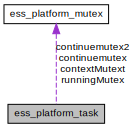
\includegraphics[width=206pt]{dd/d0e/structess__platform__task__coll__graph}
\end{center}
\end{figure}
\subsection*{Data Fields}
\begin{DoxyCompactItemize}
\item 
char \hyperlink{structess__platform__task_acd328517a6cf718155c2e6e22b671ca9}{name} \mbox{[}16\mbox{]}
\item 
int \hyperlink{structess__platform__task_a24913131dc491a81c23f2b8246d85e3b}{task\+\_\+id}
\item 
void $\ast$ \hyperlink{structess__platform__task_afd0ffb02780e738d4c0a10ab833b7834}{userdata}
\item 
void $\ast$ \hyperlink{structess__platform__task_adb63250f3f4a729239fc7335f8773cf2}{parem}
\item 
unsigned int \hyperlink{structess__platform__task_adde5266300e9cdd7ca1134daba9adf24}{stack\+\_\+size}
\item 
void $\ast$ \hyperlink{structess__platform__task_a81011b79683fab64ce3aff71114f8fdd}{handle}
\item 
int \hyperlink{structess__platform__task_acec9ce2df15222151ad66fcb1d74eb9f}{priority}
\item 
int \hyperlink{structess__platform__task_a2f45113638a0b749a8a205d2cd7fb42b}{running}
\item 
\hyperlink{ess__mutex_8h_a35346d1f106b60abe884a13846173479}{ess\+\_\+platform\+\_\+mutex\+\_\+t} \hyperlink{structess__platform__task_a9580906913a08d567aa0f7bc5b7c4150}{running\+Mutex}
\item 
\hyperlink{ess__mutex_8h_a35346d1f106b60abe884a13846173479}{ess\+\_\+platform\+\_\+mutex\+\_\+t} \hyperlink{structess__platform__task_af2a0b7dedca1f101c06a331d6e92b922}{context\+Mutext}
\item 
\hyperlink{ess__mutex_8h_a35346d1f106b60abe884a13846173479}{ess\+\_\+platform\+\_\+mutex\+\_\+t} \hyperlink{structess__platform__task_a22236d8d184eb7c41039a86bcf792380}{continuemutex}
\item 
\hyperlink{ess__mutex_8h_a35346d1f106b60abe884a13846173479}{ess\+\_\+platform\+\_\+mutex\+\_\+t} \hyperlink{structess__platform__task_afecd89745e3e4fa778a0bc75e57a5b6c}{continuemutex2}
\item 
void($\ast$ \hyperlink{structess__platform__task_a66859f9ee9fc430e9bf28644aea7c5c7}{task\+\_\+stub} )(void $\ast$data)
\end{DoxyCompactItemize}


\subsection{Detailed Description}


Definition at line 37 of file ess\+\_\+task.\+h.



\subsection{Field Documentation}
\mbox{\Hypertarget{structess__platform__task_af2a0b7dedca1f101c06a331d6e92b922}\label{structess__platform__task_af2a0b7dedca1f101c06a331d6e92b922}} 
\index{ess\+\_\+platform\+\_\+task@{ess\+\_\+platform\+\_\+task}!context\+Mutext@{context\+Mutext}}
\index{context\+Mutext@{context\+Mutext}!ess\+\_\+platform\+\_\+task@{ess\+\_\+platform\+\_\+task}}
\subsubsection{\texorpdfstring{context\+Mutext}{contextMutext}}
{\footnotesize\ttfamily \hyperlink{ess__mutex_8h_a35346d1f106b60abe884a13846173479}{ess\+\_\+platform\+\_\+mutex\+\_\+t} context\+Mutext}



Definition at line 49 of file ess\+\_\+task.\+h.

\mbox{\Hypertarget{structess__platform__task_a22236d8d184eb7c41039a86bcf792380}\label{structess__platform__task_a22236d8d184eb7c41039a86bcf792380}} 
\index{ess\+\_\+platform\+\_\+task@{ess\+\_\+platform\+\_\+task}!continuemutex@{continuemutex}}
\index{continuemutex@{continuemutex}!ess\+\_\+platform\+\_\+task@{ess\+\_\+platform\+\_\+task}}
\subsubsection{\texorpdfstring{continuemutex}{continuemutex}}
{\footnotesize\ttfamily \hyperlink{ess__mutex_8h_a35346d1f106b60abe884a13846173479}{ess\+\_\+platform\+\_\+mutex\+\_\+t} continuemutex}



Definition at line 50 of file ess\+\_\+task.\+h.

\mbox{\Hypertarget{structess__platform__task_afecd89745e3e4fa778a0bc75e57a5b6c}\label{structess__platform__task_afecd89745e3e4fa778a0bc75e57a5b6c}} 
\index{ess\+\_\+platform\+\_\+task@{ess\+\_\+platform\+\_\+task}!continuemutex2@{continuemutex2}}
\index{continuemutex2@{continuemutex2}!ess\+\_\+platform\+\_\+task@{ess\+\_\+platform\+\_\+task}}
\subsubsection{\texorpdfstring{continuemutex2}{continuemutex2}}
{\footnotesize\ttfamily \hyperlink{ess__mutex_8h_a35346d1f106b60abe884a13846173479}{ess\+\_\+platform\+\_\+mutex\+\_\+t} continuemutex2}



Definition at line 51 of file ess\+\_\+task.\+h.

\mbox{\Hypertarget{structess__platform__task_a81011b79683fab64ce3aff71114f8fdd}\label{structess__platform__task_a81011b79683fab64ce3aff71114f8fdd}} 
\index{ess\+\_\+platform\+\_\+task@{ess\+\_\+platform\+\_\+task}!handle@{handle}}
\index{handle@{handle}!ess\+\_\+platform\+\_\+task@{ess\+\_\+platform\+\_\+task}}
\subsubsection{\texorpdfstring{handle}{handle}}
{\footnotesize\ttfamily void$\ast$ handle}



Definition at line 44 of file ess\+\_\+task.\+h.

\mbox{\Hypertarget{structess__platform__task_acd328517a6cf718155c2e6e22b671ca9}\label{structess__platform__task_acd328517a6cf718155c2e6e22b671ca9}} 
\index{ess\+\_\+platform\+\_\+task@{ess\+\_\+platform\+\_\+task}!name@{name}}
\index{name@{name}!ess\+\_\+platform\+\_\+task@{ess\+\_\+platform\+\_\+task}}
\subsubsection{\texorpdfstring{name}{name}}
{\footnotesize\ttfamily char name\mbox{[}16\mbox{]}}



Definition at line 38 of file ess\+\_\+task.\+h.

\mbox{\Hypertarget{structess__platform__task_adb63250f3f4a729239fc7335f8773cf2}\label{structess__platform__task_adb63250f3f4a729239fc7335f8773cf2}} 
\index{ess\+\_\+platform\+\_\+task@{ess\+\_\+platform\+\_\+task}!parem@{parem}}
\index{parem@{parem}!ess\+\_\+platform\+\_\+task@{ess\+\_\+platform\+\_\+task}}
\subsubsection{\texorpdfstring{parem}{parem}}
{\footnotesize\ttfamily void$\ast$ parem}



Definition at line 42 of file ess\+\_\+task.\+h.

\mbox{\Hypertarget{structess__platform__task_acec9ce2df15222151ad66fcb1d74eb9f}\label{structess__platform__task_acec9ce2df15222151ad66fcb1d74eb9f}} 
\index{ess\+\_\+platform\+\_\+task@{ess\+\_\+platform\+\_\+task}!priority@{priority}}
\index{priority@{priority}!ess\+\_\+platform\+\_\+task@{ess\+\_\+platform\+\_\+task}}
\subsubsection{\texorpdfstring{priority}{priority}}
{\footnotesize\ttfamily int priority}



Definition at line 45 of file ess\+\_\+task.\+h.

\mbox{\Hypertarget{structess__platform__task_a2f45113638a0b749a8a205d2cd7fb42b}\label{structess__platform__task_a2f45113638a0b749a8a205d2cd7fb42b}} 
\index{ess\+\_\+platform\+\_\+task@{ess\+\_\+platform\+\_\+task}!running@{running}}
\index{running@{running}!ess\+\_\+platform\+\_\+task@{ess\+\_\+platform\+\_\+task}}
\subsubsection{\texorpdfstring{running}{running}}
{\footnotesize\ttfamily int running}



Definition at line 46 of file ess\+\_\+task.\+h.

\mbox{\Hypertarget{structess__platform__task_a9580906913a08d567aa0f7bc5b7c4150}\label{structess__platform__task_a9580906913a08d567aa0f7bc5b7c4150}} 
\index{ess\+\_\+platform\+\_\+task@{ess\+\_\+platform\+\_\+task}!running\+Mutex@{running\+Mutex}}
\index{running\+Mutex@{running\+Mutex}!ess\+\_\+platform\+\_\+task@{ess\+\_\+platform\+\_\+task}}
\subsubsection{\texorpdfstring{running\+Mutex}{runningMutex}}
{\footnotesize\ttfamily \hyperlink{ess__mutex_8h_a35346d1f106b60abe884a13846173479}{ess\+\_\+platform\+\_\+mutex\+\_\+t} running\+Mutex}



Definition at line 48 of file ess\+\_\+task.\+h.

\mbox{\Hypertarget{structess__platform__task_adde5266300e9cdd7ca1134daba9adf24}\label{structess__platform__task_adde5266300e9cdd7ca1134daba9adf24}} 
\index{ess\+\_\+platform\+\_\+task@{ess\+\_\+platform\+\_\+task}!stack\+\_\+size@{stack\+\_\+size}}
\index{stack\+\_\+size@{stack\+\_\+size}!ess\+\_\+platform\+\_\+task@{ess\+\_\+platform\+\_\+task}}
\subsubsection{\texorpdfstring{stack\+\_\+size}{stack\_size}}
{\footnotesize\ttfamily unsigned int stack\+\_\+size}



Definition at line 43 of file ess\+\_\+task.\+h.

\mbox{\Hypertarget{structess__platform__task_a24913131dc491a81c23f2b8246d85e3b}\label{structess__platform__task_a24913131dc491a81c23f2b8246d85e3b}} 
\index{ess\+\_\+platform\+\_\+task@{ess\+\_\+platform\+\_\+task}!task\+\_\+id@{task\+\_\+id}}
\index{task\+\_\+id@{task\+\_\+id}!ess\+\_\+platform\+\_\+task@{ess\+\_\+platform\+\_\+task}}
\subsubsection{\texorpdfstring{task\+\_\+id}{task\_id}}
{\footnotesize\ttfamily int task\+\_\+id}



Definition at line 39 of file ess\+\_\+task.\+h.

\mbox{\Hypertarget{structess__platform__task_a66859f9ee9fc430e9bf28644aea7c5c7}\label{structess__platform__task_a66859f9ee9fc430e9bf28644aea7c5c7}} 
\index{ess\+\_\+platform\+\_\+task@{ess\+\_\+platform\+\_\+task}!task\+\_\+stub@{task\+\_\+stub}}
\index{task\+\_\+stub@{task\+\_\+stub}!ess\+\_\+platform\+\_\+task@{ess\+\_\+platform\+\_\+task}}
\subsubsection{\texorpdfstring{task\+\_\+stub}{task\_stub}}
{\footnotesize\ttfamily void($\ast$  task\+\_\+stub) (void $\ast$data)}



Definition at line 53 of file ess\+\_\+task.\+h.

\mbox{\Hypertarget{structess__platform__task_afd0ffb02780e738d4c0a10ab833b7834}\label{structess__platform__task_afd0ffb02780e738d4c0a10ab833b7834}} 
\index{ess\+\_\+platform\+\_\+task@{ess\+\_\+platform\+\_\+task}!userdata@{userdata}}
\index{userdata@{userdata}!ess\+\_\+platform\+\_\+task@{ess\+\_\+platform\+\_\+task}}
\subsubsection{\texorpdfstring{userdata}{userdata}}
{\footnotesize\ttfamily void$\ast$ userdata}



Definition at line 41 of file ess\+\_\+task.\+h.



The documentation for this struct was generated from the following file\+:\begin{DoxyCompactItemize}
\item 
include/\hyperlink{ess__task_8h}{ess\+\_\+task.\+h}\end{DoxyCompactItemize}

\hypertarget{structess__server}{}\section{ess\+\_\+server Struct Reference}
\label{structess__server}\index{ess\+\_\+server@{ess\+\_\+server}}


{\ttfamily \#include $<$server.\+h$>$}

\subsection*{Data Fields}
\begin{DoxyCompactItemize}
\item 
const char $\ast$ \hyperlink{structess__server_aad01339e89106fdf68f57ef118956fa9}{hostname}
\item 
ess\+\_\+backend\+\_\+t $\ast$ \hyperlink{structess__server_ab2b85d146ada2907a81371aace6e926d}{backend}
\item 
\hyperlink{ess__format_8h_ab03f24cb5d42f4448f713bf1ec178163}{ess\+\_\+format\+\_\+t} \hyperlink{structess__server_abb4395d1c05d3bbc2e1d011507ddd19b}{format}
\item 
int \hyperlink{structess__server_a63c89c04d1feae07ca35558055155ffb}{port}
\item 
int \hyperlink{structess__server_a3666576f6b88007cc7b8f26c7da596c8}{socket}
\item 
void $\ast$ \hyperlink{structess__server_a368f7094dc38acca20612bbb392552f4}{buffer}
\item 
int \hyperlink{structess__server_a1aa199bcd52f6acf8edbf2ee6898a21b}{magl}
\item 
int \hyperlink{structess__server_a64b10d79850e935f9440886335b9f391}{magr}
\item 
int \hyperlink{structess__server_a218b4f7c6cc2681a99c23a3b089d68b1}{speed}
\item 
int \hyperlink{structess__server_a9f59b34b1f25fe00023291b678246bcc}{length}
\item 
int \hyperlink{structess__server_aed7ea92f45bd273dde380a45ddced592}{offset}
\item 
\hyperlink{server_8h_a66019638fd44eba9d951ec93754c7b8d}{ess\+\_\+server\+\_\+status\+\_\+t} \hyperlink{structess__server_af34befa103928930a907b2eb5cc4739c}{status}
\end{DoxyCompactItemize}


\subsection{Detailed Description}


Definition at line 18 of file server.\+h.



\subsection{Field Documentation}
\mbox{\Hypertarget{structess__server_ab2b85d146ada2907a81371aace6e926d}\label{structess__server_ab2b85d146ada2907a81371aace6e926d}} 
\index{ess\+\_\+server@{ess\+\_\+server}!backend@{backend}}
\index{backend@{backend}!ess\+\_\+server@{ess\+\_\+server}}
\subsubsection{\texorpdfstring{backend}{backend}}
{\footnotesize\ttfamily ess\+\_\+backend\+\_\+t$\ast$ backend}



Definition at line 20 of file server.\+h.

\mbox{\Hypertarget{structess__server_a368f7094dc38acca20612bbb392552f4}\label{structess__server_a368f7094dc38acca20612bbb392552f4}} 
\index{ess\+\_\+server@{ess\+\_\+server}!buffer@{buffer}}
\index{buffer@{buffer}!ess\+\_\+server@{ess\+\_\+server}}
\subsubsection{\texorpdfstring{buffer}{buffer}}
{\footnotesize\ttfamily void$\ast$ buffer}



Definition at line 25 of file server.\+h.

\mbox{\Hypertarget{structess__server_abb4395d1c05d3bbc2e1d011507ddd19b}\label{structess__server_abb4395d1c05d3bbc2e1d011507ddd19b}} 
\index{ess\+\_\+server@{ess\+\_\+server}!format@{format}}
\index{format@{format}!ess\+\_\+server@{ess\+\_\+server}}
\subsubsection{\texorpdfstring{format}{format}}
{\footnotesize\ttfamily \hyperlink{ess__format_8h_ab03f24cb5d42f4448f713bf1ec178163}{ess\+\_\+format\+\_\+t} format}



Definition at line 21 of file server.\+h.

\mbox{\Hypertarget{structess__server_aad01339e89106fdf68f57ef118956fa9}\label{structess__server_aad01339e89106fdf68f57ef118956fa9}} 
\index{ess\+\_\+server@{ess\+\_\+server}!hostname@{hostname}}
\index{hostname@{hostname}!ess\+\_\+server@{ess\+\_\+server}}
\subsubsection{\texorpdfstring{hostname}{hostname}}
{\footnotesize\ttfamily const char$\ast$ hostname}



Definition at line 19 of file server.\+h.

\mbox{\Hypertarget{structess__server_a9f59b34b1f25fe00023291b678246bcc}\label{structess__server_a9f59b34b1f25fe00023291b678246bcc}} 
\index{ess\+\_\+server@{ess\+\_\+server}!length@{length}}
\index{length@{length}!ess\+\_\+server@{ess\+\_\+server}}
\subsubsection{\texorpdfstring{length}{length}}
{\footnotesize\ttfamily int length}



Definition at line 27 of file server.\+h.

\mbox{\Hypertarget{structess__server_a1aa199bcd52f6acf8edbf2ee6898a21b}\label{structess__server_a1aa199bcd52f6acf8edbf2ee6898a21b}} 
\index{ess\+\_\+server@{ess\+\_\+server}!magl@{magl}}
\index{magl@{magl}!ess\+\_\+server@{ess\+\_\+server}}
\subsubsection{\texorpdfstring{magl}{magl}}
{\footnotesize\ttfamily int magl}



Definition at line 26 of file server.\+h.

\mbox{\Hypertarget{structess__server_a64b10d79850e935f9440886335b9f391}\label{structess__server_a64b10d79850e935f9440886335b9f391}} 
\index{ess\+\_\+server@{ess\+\_\+server}!magr@{magr}}
\index{magr@{magr}!ess\+\_\+server@{ess\+\_\+server}}
\subsubsection{\texorpdfstring{magr}{magr}}
{\footnotesize\ttfamily int magr}



Definition at line 26 of file server.\+h.

\mbox{\Hypertarget{structess__server_aed7ea92f45bd273dde380a45ddced592}\label{structess__server_aed7ea92f45bd273dde380a45ddced592}} 
\index{ess\+\_\+server@{ess\+\_\+server}!offset@{offset}}
\index{offset@{offset}!ess\+\_\+server@{ess\+\_\+server}}
\subsubsection{\texorpdfstring{offset}{offset}}
{\footnotesize\ttfamily int offset}



Definition at line 27 of file server.\+h.

\mbox{\Hypertarget{structess__server_a63c89c04d1feae07ca35558055155ffb}\label{structess__server_a63c89c04d1feae07ca35558055155ffb}} 
\index{ess\+\_\+server@{ess\+\_\+server}!port@{port}}
\index{port@{port}!ess\+\_\+server@{ess\+\_\+server}}
\subsubsection{\texorpdfstring{port}{port}}
{\footnotesize\ttfamily int port}



Definition at line 22 of file server.\+h.

\mbox{\Hypertarget{structess__server_a3666576f6b88007cc7b8f26c7da596c8}\label{structess__server_a3666576f6b88007cc7b8f26c7da596c8}} 
\index{ess\+\_\+server@{ess\+\_\+server}!socket@{socket}}
\index{socket@{socket}!ess\+\_\+server@{ess\+\_\+server}}
\subsubsection{\texorpdfstring{socket}{socket}}
{\footnotesize\ttfamily int socket}



Definition at line 23 of file server.\+h.

\mbox{\Hypertarget{structess__server_a218b4f7c6cc2681a99c23a3b089d68b1}\label{structess__server_a218b4f7c6cc2681a99c23a3b089d68b1}} 
\index{ess\+\_\+server@{ess\+\_\+server}!speed@{speed}}
\index{speed@{speed}!ess\+\_\+server@{ess\+\_\+server}}
\subsubsection{\texorpdfstring{speed}{speed}}
{\footnotesize\ttfamily int speed}



Definition at line 27 of file server.\+h.

\mbox{\Hypertarget{structess__server_af34befa103928930a907b2eb5cc4739c}\label{structess__server_af34befa103928930a907b2eb5cc4739c}} 
\index{ess\+\_\+server@{ess\+\_\+server}!status@{status}}
\index{status@{status}!ess\+\_\+server@{ess\+\_\+server}}
\subsubsection{\texorpdfstring{status}{status}}
{\footnotesize\ttfamily \hyperlink{server_8h_a66019638fd44eba9d951ec93754c7b8d}{ess\+\_\+server\+\_\+status\+\_\+t} status}



Definition at line 29 of file server.\+h.



The documentation for this struct was generated from the following file\+:\begin{DoxyCompactItemize}
\item 
include/\hyperlink{server_8h}{server.\+h}\end{DoxyCompactItemize}

\hypertarget{structess__socket}{}\section{ess\+\_\+socket Struct Reference}
\label{structess__socket}\index{ess\+\_\+socket@{ess\+\_\+socket}}


hold all socket managment importend data  




{\ttfamily \#include $<$ess\+\_\+socket.\+h$>$}

\subsection*{Data Fields}
\begin{DoxyCompactItemize}
\item 
char \hyperlink{structess__socket_a0c6be700c8763c26054098348ebef8d6}{hostname} \mbox{[}64\mbox{]}
\item 
unsigned int \hyperlink{structess__socket_a4d0d74743d167680649419163ce8c80e}{hostname\+\_\+len}
\item 
unsigned int \hyperlink{structess__socket_a938bdc6ae46c346147b6d4f67ad1e704}{port}
\item 
int \hyperlink{structess__socket_a3666576f6b88007cc7b8f26c7da596c8}{socket}
\item 
int \hyperlink{structess__socket_a7f345697df7eb20c9aba1ab6980cae8f}{retval}
\item 
\hyperlink{ess__socket_8h_a1e8e8de805f8e0b7da25e3b177977273}{ess\+\_\+socket\+\_\+pro\+\_\+t} \hyperlink{structess__socket_a1f0429596710512357072b192ba3d2bd}{protokol}
\item 
\hyperlink{ess__socket_8h_a9305eae437d57846661e997bb755d150}{ess\+\_\+socket\+\_\+fam\+\_\+t} \hyperlink{structess__socket_ad09623d57ebd33fef8dac4e18c0cba2f}{family}
\item 
\hyperlink{ess__socket_8h_ae3a6dc482fc34f9ea0361820ba4be573}{ess\+\_\+socket\+\_\+status\+\_\+t} \hyperlink{structess__socket_a4e47521e8af756b9edf77f1f02f9b725}{status}
\end{DoxyCompactItemize}


\subsection{Detailed Description}
hold all socket managment importend data 

Definition at line 82 of file ess\+\_\+socket.\+h.



\subsection{Field Documentation}
\mbox{\Hypertarget{structess__socket_ad09623d57ebd33fef8dac4e18c0cba2f}\label{structess__socket_ad09623d57ebd33fef8dac4e18c0cba2f}} 
\index{ess\+\_\+socket@{ess\+\_\+socket}!family@{family}}
\index{family@{family}!ess\+\_\+socket@{ess\+\_\+socket}}
\subsubsection{\texorpdfstring{family}{family}}
{\footnotesize\ttfamily \hyperlink{ess__socket_8h_a9305eae437d57846661e997bb755d150}{ess\+\_\+socket\+\_\+fam\+\_\+t} family}

{\ttfamily E\+S\+S\+\_\+\+S\+O\+C\+K\+E\+T\+\_\+\+F\+A\+M\+I\+L\+Y\+\_\+\+I\+P4}, {\ttfamily E\+S\+S\+\_\+\+S\+O\+C\+K\+E\+T\+\_\+\+F\+A\+M\+I\+L\+Y\+\_\+\+I\+P6} or {\ttfamily E\+S\+S\+\_\+\+S\+O\+C\+K\+E\+T\+\_\+\+F\+A\+M\+I\+L\+Y\+\_\+\+B\+O\+TH}; latter means that the D\+NS resolver should decide. 

Definition at line 90 of file ess\+\_\+socket.\+h.

\mbox{\Hypertarget{structess__socket_a0c6be700c8763c26054098348ebef8d6}\label{structess__socket_a0c6be700c8763c26054098348ebef8d6}} 
\index{ess\+\_\+socket@{ess\+\_\+socket}!hostname@{hostname}}
\index{hostname@{hostname}!ess\+\_\+socket@{ess\+\_\+socket}}
\subsubsection{\texorpdfstring{hostname}{hostname}}
{\footnotesize\ttfamily char hostname\mbox{[}64\mbox{]}}

Address to bind or client hostname. If you want to bind to every address use \char`\"{}0.\+0.\+0.\+0\char`\"{} or \char`\"{}\+::\char`\"{} (I\+Pv6 wildcard) 

Definition at line 83 of file ess\+\_\+socket.\+h.

\mbox{\Hypertarget{structess__socket_a4d0d74743d167680649419163ce8c80e}\label{structess__socket_a4d0d74743d167680649419163ce8c80e}} 
\index{ess\+\_\+socket@{ess\+\_\+socket}!hostname\+\_\+len@{hostname\+\_\+len}}
\index{hostname\+\_\+len@{hostname\+\_\+len}!ess\+\_\+socket@{ess\+\_\+socket}}
\subsubsection{\texorpdfstring{hostname\+\_\+len}{hostname\_len}}
{\footnotesize\ttfamily unsigned int hostname\+\_\+len}



Definition at line 84 of file ess\+\_\+socket.\+h.

\mbox{\Hypertarget{structess__socket_a938bdc6ae46c346147b6d4f67ad1e704}\label{structess__socket_a938bdc6ae46c346147b6d4f67ad1e704}} 
\index{ess\+\_\+socket@{ess\+\_\+socket}!port@{port}}
\index{port@{port}!ess\+\_\+socket@{ess\+\_\+socket}}
\subsubsection{\texorpdfstring{port}{port}}
{\footnotesize\ttfamily unsigned int port}

$<$ hostname length The port to bind. 

Definition at line 85 of file ess\+\_\+socket.\+h.

\mbox{\Hypertarget{structess__socket_a1f0429596710512357072b192ba3d2bd}\label{structess__socket_a1f0429596710512357072b192ba3d2bd}} 
\index{ess\+\_\+socket@{ess\+\_\+socket}!protokol@{protokol}}
\index{protokol@{protokol}!ess\+\_\+socket@{ess\+\_\+socket}}
\subsubsection{\texorpdfstring{protokol}{protokol}}
{\footnotesize\ttfamily \hyperlink{ess__socket_8h_a1e8e8de805f8e0b7da25e3b177977273}{ess\+\_\+socket\+\_\+pro\+\_\+t} protokol}

{\ttfamily E\+S\+S\+\_\+\+S\+O\+C\+K\+E\+T\+\_\+\+P\+R\+O\+T\+O\+\_\+\+S\+T\+R\+E\+AM}, {\ttfamily E\+S\+S\+\_\+\+S\+O\+C\+K\+E\+T\+\_\+\+P\+R\+O\+T\+O\+\_\+\+D\+R\+AM} or {\ttfamily E\+S\+S\+\_\+\+S\+O\+C\+K\+E\+T\+\_\+\+P\+R\+O\+T\+O\+\_\+\+D\+R\+A\+M\+\_\+\+L\+I\+TE} -\/ the using protokoll 

Definition at line 89 of file ess\+\_\+socket.\+h.

\mbox{\Hypertarget{structess__socket_a7f345697df7eb20c9aba1ab6980cae8f}\label{structess__socket_a7f345697df7eb20c9aba1ab6980cae8f}} 
\index{ess\+\_\+socket@{ess\+\_\+socket}!retval@{retval}}
\index{retval@{retval}!ess\+\_\+socket@{ess\+\_\+socket}}
\subsubsection{\texorpdfstring{retval}{retval}}
{\footnotesize\ttfamily int retval}



Definition at line 88 of file ess\+\_\+socket.\+h.

\mbox{\Hypertarget{structess__socket_a3666576f6b88007cc7b8f26c7da596c8}\label{structess__socket_a3666576f6b88007cc7b8f26c7da596c8}} 
\index{ess\+\_\+socket@{ess\+\_\+socket}!socket@{socket}}
\index{socket@{socket}!ess\+\_\+socket@{ess\+\_\+socket}}
\subsubsection{\texorpdfstring{socket}{socket}}
{\footnotesize\ttfamily int socket}

The socket 

Definition at line 87 of file ess\+\_\+socket.\+h.

\mbox{\Hypertarget{structess__socket_a4e47521e8af756b9edf77f1f02f9b725}\label{structess__socket_a4e47521e8af756b9edf77f1f02f9b725}} 
\index{ess\+\_\+socket@{ess\+\_\+socket}!status@{status}}
\index{status@{status}!ess\+\_\+socket@{ess\+\_\+socket}}
\subsubsection{\texorpdfstring{status}{status}}
{\footnotesize\ttfamily \hyperlink{ess__socket_8h_ae3a6dc482fc34f9ea0361820ba4be573}{ess\+\_\+socket\+\_\+status\+\_\+t} status}

\hyperlink{structess__socket}{ess\+\_\+socket} status 

Definition at line 91 of file ess\+\_\+socket.\+h.



The documentation for this struct was generated from the following file\+:\begin{DoxyCompactItemize}
\item 
include/\hyperlink{ess__socket_8h}{ess\+\_\+socket.\+h}\end{DoxyCompactItemize}

\chapter{File Documentation}
\input{d2/da7/_c_o_n_t_r_i_b_u_t_i_n_g_8md}
\hypertarget{config_8h}{}\section{include/config.h File Reference}
\label{config_8h}\index{include/config.\+h@{include/config.\+h}}


File containing configurations.  


This graph shows which files directly or indirectly include this file\+:
\nopagebreak
\begin{figure}[H]
\begin{center}
\leavevmode
\includegraphics[width=350pt]{d0/dbc/config_8h__dep__incl}
\end{center}
\end{figure}
\subsection*{Macros}
\begin{DoxyCompactItemize}
\item 
\#define \hyperlink{config_8h_a864c702c32ff878dfae80901d18b5e6b}{E\+S\+S\+\_\+\+P\+R\+O\+T\+O\+C\+O\+L\+\_\+\+U\+DP}~1
\item 
\#define \hyperlink{config_8h_aa2779759502a5e8e231dd70c80d2fab4}{E\+S\+S\+\_\+\+P\+R\+O\+T\+O\+C\+O\+L\+\_\+\+T\+CP}~2
\item 
\#define \hyperlink{config_8h_a9381900ab9e06304b63260e80e02a74e}{E\+S\+S\+\_\+\+P\+R\+O\+T\+O\+C\+O\+L\+\_\+\+U\+D\+P\+\_\+\+L\+I\+TE}~3
\item 
\#define \hyperlink{config_8h_a08a4d2f56e8589e98112a8bc6282e1b3}{E\+S\+S\+\_\+\+F\+A\+M\+I\+L\+Y\+\_\+\+I\+P4}~4
\item 
\#define \hyperlink{config_8h_a88a58bb0c53e91e2e1da83d39be65577}{E\+S\+S\+\_\+\+F\+A\+M\+I\+L\+Y\+\_\+\+I\+P6}~6
\item 
\#define \hyperlink{config_8h_a3f3bdcf7dca164338ad07976edb214a9}{E\+S\+S\+\_\+\+F\+A\+M\+I\+L\+Y\+\_\+\+B\+O\+TH}~46
\item 
\#define \hyperlink{config_8h_a3f389a7d9b38a23281f85044251d3e5c}{E\+S\+S\+\_\+\+P\+L\+A\+T\+F\+O\+R\+M\+\_\+\+E\+S\+P32}~/$\ast$$\ast$ @brief If defined compiled backend for esp32 $\ast$/
\item 
\#define \hyperlink{config_8h_a1f818721e5dfb42af99b1fede72e3d79}{E\+S\+S\+\_\+\+D\+E\+F\+A\+U\+L\+T\+\_\+\+S\+E\+R\+V\+E\+R\+\_\+\+P\+O\+RT}~16001
\item 
\#define \hyperlink{config_8h_afa519d17d6eba4da4ccd710c8f046469}{E\+S\+S\+\_\+\+D\+E\+F\+A\+U\+L\+T\+\_\+\+S\+E\+R\+V\+E\+R\+\_\+\+P\+R\+O\+T\+O\+C\+OL}~\hyperlink{config_8h_aa2779759502a5e8e231dd70c80d2fab4}{E\+S\+S\+\_\+\+P\+R\+O\+T\+O\+C\+O\+L\+\_\+\+T\+CP}
\item 
\#define \hyperlink{config_8h_a8160742d1b6ff1af73cea9904bfb8d80}{E\+S\+S\+\_\+\+D\+E\+F\+A\+U\+L\+T\+\_\+\+S\+E\+R\+V\+E\+R\+\_\+\+F\+A\+M\+I\+LY}~\hyperlink{config_8h_a88a58bb0c53e91e2e1da83d39be65577}{E\+S\+S\+\_\+\+F\+A\+M\+I\+L\+Y\+\_\+\+I\+P6}
\item 
\#define \hyperlink{config_8h_ab23cc2c3901ed56c7f9c01c9ddaaf8bb}{E\+S\+S\+\_\+\+D\+E\+F\+A\+U\+L\+T\+\_\+\+S\+E\+R\+V\+E\+R\+\_\+\+H\+O\+ST}~\char`\"{}\+::\char`\"{}
\item 
\#define \hyperlink{config_8h_aba25849ddf4184eaa3f9ee8e7df64939}{E\+S\+S\+\_\+\+C\+O\+N\+F\+I\+G\+\_\+\+S\+E\+M\+A\+P\+H\+O\+R\+E\+\_\+\+G\+E\+N\+E\+R\+IC}
\item 
\#define \hyperlink{config_8h_a38fbb177b38ddb77d210352bfa057f8d}{E\+S\+S\+\_\+\+C\+O\+N\+F\+I\+C\+\_\+\+T\+A\+S\+K\+\_\+\+E\+S\+P32}
\item 
\#define \hyperlink{config_8h_adfe2386980d49f63c523d8f6ca387bfc}{E\+S\+S\+\_\+\+C\+O\+N\+F\+I\+G\+\_\+\+R\+I\+N\+G\+B\+U\+F\+F\+E\+R\+\_\+\+E\+S\+P32}
\item 
\#define \hyperlink{config_8h_a8ebad82a88be2263389cd34854665c51}{E\+S\+S\+\_\+\+C\+O\+N\+F\+I\+G\+\_\+\+M\+U\+T\+E\+X\+\_\+\+E\+S\+P32}
\item 
\#define \hyperlink{config_8h_a3a4802a9e6f7f6028e532a84ea13146a}{E\+S\+S\+\_\+\+C\+O\+N\+F\+I\+G\+\_\+\+S\+P\+I\+N\+L\+O\+C\+K\+\_\+\+E\+S\+P32}
\item 
\#define \hyperlink{config_8h_a932ce0db7f54e163e3648750e5dc974d}{E\+S\+S\+\_\+\+E\+N\+A\+B\+L\+E\+\_\+\+B\+A\+C\+K\+E\+N\+D\+\_\+\+U\+A\+RT}
\begin{DoxyCompactList}\small\item\em If defined then U\+A\+RT backend available. \end{DoxyCompactList}\item 
\#define \hyperlink{config_8h_af06555cb35471d5f34b810a91a745180}{E\+S\+S\+\_\+\+E\+N\+A\+B\+L\+E\+\_\+\+B\+A\+C\+K\+E\+N\+D\+\_\+\+I2S}
\begin{DoxyCompactList}\small\item\em If defined then I2S backend available. \end{DoxyCompactList}\item 
\#define \hyperlink{config_8h_a6387906bbd088f14df3dddfbff20ca6a}{E\+S\+S\+\_\+\+E\+N\+A\+B\+L\+E\+\_\+\+B\+A\+C\+K\+E\+N\+D\+\_\+\+U\+DP}
\begin{DoxyCompactList}\small\item\em If defined then U\+DP backend available. \end{DoxyCompactList}\item 
\#define \hyperlink{config_8h_aa273d0e3f100e575a28b9c4dafcc7e91}{E\+S\+S\+\_\+\+D\+E\+F\+A\+U\+L\+T\+\_\+\+S\+E\+R\+V\+E\+R\+\_\+\+N\+A\+ME}~\char`\"{}Open\+EssD-\/esp32\char`\"{}
\item 
\#define \hyperlink{config_8h_a877be7a5994da0fbc4a90fc0d2a55dd4}{E\+S\+S\+\_\+\+B\+A\+C\+K\+E\+N\+D\+\_\+\+U\+A\+R\+T\+\_\+\+B\+A\+U\+D\+R\+AT}~115200
\item 
\#define \hyperlink{config_8h_a31e66e9e78324a884ef420474ec7565c}{E\+S\+S\+\_\+\+B\+A\+C\+K\+E\+N\+D\+\_\+\+U\+A\+R\+T\+\_\+\+T\+XD}~(G\+P\+I\+O\+\_\+\+N\+U\+M\+\_\+4)
\item 
\#define \hyperlink{config_8h_a29270f90b4c19c90c4bcbccf7000028f}{E\+S\+S\+\_\+\+B\+A\+C\+K\+E\+N\+D\+\_\+\+U\+A\+R\+T\+\_\+\+R\+XD}~(G\+P\+I\+O\+\_\+\+N\+U\+M\+\_\+5)
\item 
\#define \hyperlink{config_8h_ac892535bab324b6ba680ab071adca204}{E\+S\+S\+\_\+\+B\+A\+C\+K\+E\+N\+D\+\_\+\+U\+A\+R\+T\+\_\+\+R\+TS}~(U\+A\+R\+T\+\_\+\+P\+I\+N\+\_\+\+N\+O\+\_\+\+C\+H\+A\+N\+GE)
\item 
\#define \hyperlink{config_8h_ad9feb54c36cd8108c9783d51417f2f20}{E\+S\+S\+\_\+\+B\+A\+C\+K\+E\+N\+D\+\_\+\+U\+A\+R\+T\+\_\+\+C\+TS}~(U\+A\+R\+T\+\_\+\+P\+I\+N\+\_\+\+N\+O\+\_\+\+C\+H\+A\+N\+GE)
\item 
\#define \hyperlink{config_8h_a8cf3fc0a0687282fd85ebdcc7442a12c}{E\+S\+S\+\_\+\+B\+A\+C\+K\+E\+N\+D\+\_\+\+U\+D\+P\+\_\+\+P\+O\+RT}~17000
\item 
\#define \hyperlink{config_8h_ac7a68418b14fc943a7a254afed0465fd}{E\+S\+S\+\_\+\+B\+A\+C\+K\+E\+N\+D\+\_\+\+U\+D\+P\+\_\+\+H\+O\+ST}~192.\+168.\+0.\+235
\item 
\#define \hyperlink{config_8h_a5c67295f81f12a8d932b66e828512493}{E\+S\+S\+\_\+\+B\+A\+C\+K\+E\+N\+D\+\_\+\+U\+D\+P\+\_\+\+F\+A\+M\+I\+LY}~\hyperlink{config_8h_a3f3bdcf7dca164338ad07976edb214a9}{E\+S\+S\+\_\+\+F\+A\+M\+I\+L\+Y\+\_\+\+B\+O\+TH}
\item 
\#define \hyperlink{config_8h_ab826493b5676da2fa30ecd16e4213cca}{I2\+S\+\_\+\+E\+X\+T\+E\+R\+N\+A\+L\+\_\+\+D\+A\+C\+\_\+\+B\+CK}~26
\item 
\#define \hyperlink{config_8h_aec220c9a7472c9bf1257d587a1f5de78}{I2\+S\+\_\+\+E\+X\+T\+E\+R\+N\+A\+L\+\_\+\+D\+A\+C\+\_\+\+L\+R\+C\+LK}~25
\item 
\#define \hyperlink{config_8h_aa401441e2cd997ee4341164a391d0d7b}{I2\+S\+\_\+\+E\+X\+T\+E\+R\+N\+A\+L\+\_\+\+D\+A\+C\+\_\+\+D\+O\+UT}~22
\item 
\#define \hyperlink{config_8h_aa1a44ddac06dbb7a26467b553151edfc}{I2\+S\+\_\+\+E\+X\+T\+E\+R\+N\+A\+L\+\_\+\+D\+A\+C\+\_\+\+D\+IN}~-\/1
\item 
\#define \hyperlink{config_8h_a6006e6b6eac0e38b977816a742b23e03}{E\+S\+S\+\_\+\+B\+A\+C\+K\+E\+N\+D\+\_\+\+I2\+S\+\_\+\+F\+O\+R\+M\+AT}~\hyperlink{ess__format_8h_aa73ee1bade9564053c023e42c9ea1ec9a95f4383e32c5243da6c704ac89cc6ffe}{E\+S\+S\+\_\+\+F\+O\+R\+M\+A\+T\+\_\+\+S\+T\+E\+R\+E\+O\+\_\+96000\+\_\+16}
\item 
\#define \hyperlink{config_8h_ad6244925ccbfe20b1bb5fea5b5fee1f6}{E\+S\+S\+\_\+\+B\+A\+C\+K\+E\+N\+D\+\_\+\+I2\+S\+\_\+\+D\+M\+A\+\_\+\+B\+U\+F\+\_\+\+S\+I\+ZE}~64
\item 
\#define \hyperlink{config_8h_a8224eac6b4f2c107702374e9e90f0bd5}{E\+S\+S\+\_\+\+B\+A\+C\+K\+E\+N\+D\+\_\+\+I2\+S\+\_\+\+D\+M\+A\+\_\+\+B\+U\+F\+\_\+\+C\+O\+U\+NT}~6
\item 
\#define \hyperlink{config_8h_a02a4eb9ca75bf77fd60b4cb7bde37f2f}{E\+S\+S\+\_\+\+B\+A\+C\+K\+E\+N\+D\+\_\+\+N\+A\+M\+E\+\_\+\+I2\+S\+\_\+\+E\+S\+P32}~\char`\"{}i2s\+\_\+esp32\char`\"{}
\item 
\#define \hyperlink{config_8h_ab49df6da13352ca7e9705c54f10e5f2f}{E\+S\+S\+\_\+\+B\+A\+C\+K\+E\+N\+D\+\_\+\+N\+A\+M\+E\+\_\+\+N\+U\+LL}~\char`\"{}null\char`\"{}
\item 
\#define \hyperlink{config_8h_a3fe797468119106c63b0cf0662750dff}{E\+S\+S\+\_\+\+B\+A\+C\+K\+E\+N\+D\+\_\+\+N\+A\+M\+E\+\_\+\+U\+DP}~\char`\"{}udp\char`\"{}
\item 
\#define \hyperlink{config_8h_a5873aa29af32bc61d7f9d96c09ba7c8b}{E\+S\+S\+\_\+\+B\+A\+C\+K\+E\+N\+D\+\_\+\+N\+A\+M\+E\+\_\+\+U\+A\+R\+T\+\_\+\+E\+S\+P32}~\char`\"{}U\+A\+R\+T\+\_\+\+E\+S\+P32\char`\"{}
\end{DoxyCompactItemize}


\subsection{Detailed Description}
File containing configurations. 

\begin{DoxyAuthor}{Author}
Anna Sopdia Schröck 
\end{DoxyAuthor}
\begin{DoxyDate}{Date}
30 Januar 20119 
\end{DoxyDate}


\subsection{Macro Definition Documentation}
\mbox{\Hypertarget{config_8h_a8224eac6b4f2c107702374e9e90f0bd5}\label{config_8h_a8224eac6b4f2c107702374e9e90f0bd5}} 
\index{config.\+h@{config.\+h}!E\+S\+S\+\_\+\+B\+A\+C\+K\+E\+N\+D\+\_\+\+I2\+S\+\_\+\+D\+M\+A\+\_\+\+B\+U\+F\+\_\+\+C\+O\+U\+NT@{E\+S\+S\+\_\+\+B\+A\+C\+K\+E\+N\+D\+\_\+\+I2\+S\+\_\+\+D\+M\+A\+\_\+\+B\+U\+F\+\_\+\+C\+O\+U\+NT}}
\index{E\+S\+S\+\_\+\+B\+A\+C\+K\+E\+N\+D\+\_\+\+I2\+S\+\_\+\+D\+M\+A\+\_\+\+B\+U\+F\+\_\+\+C\+O\+U\+NT@{E\+S\+S\+\_\+\+B\+A\+C\+K\+E\+N\+D\+\_\+\+I2\+S\+\_\+\+D\+M\+A\+\_\+\+B\+U\+F\+\_\+\+C\+O\+U\+NT}!config.\+h@{config.\+h}}
\subsubsection{\texorpdfstring{E\+S\+S\+\_\+\+B\+A\+C\+K\+E\+N\+D\+\_\+\+I2\+S\+\_\+\+D\+M\+A\+\_\+\+B\+U\+F\+\_\+\+C\+O\+U\+NT}{ESS\_BACKEND\_I2S\_DMA\_BUF\_COUNT}}
{\footnotesize\ttfamily \#define E\+S\+S\+\_\+\+B\+A\+C\+K\+E\+N\+D\+\_\+\+I2\+S\+\_\+\+D\+M\+A\+\_\+\+B\+U\+F\+\_\+\+C\+O\+U\+NT~6}



Definition at line 138 of file config.\+h.

\mbox{\Hypertarget{config_8h_ad6244925ccbfe20b1bb5fea5b5fee1f6}\label{config_8h_ad6244925ccbfe20b1bb5fea5b5fee1f6}} 
\index{config.\+h@{config.\+h}!E\+S\+S\+\_\+\+B\+A\+C\+K\+E\+N\+D\+\_\+\+I2\+S\+\_\+\+D\+M\+A\+\_\+\+B\+U\+F\+\_\+\+S\+I\+ZE@{E\+S\+S\+\_\+\+B\+A\+C\+K\+E\+N\+D\+\_\+\+I2\+S\+\_\+\+D\+M\+A\+\_\+\+B\+U\+F\+\_\+\+S\+I\+ZE}}
\index{E\+S\+S\+\_\+\+B\+A\+C\+K\+E\+N\+D\+\_\+\+I2\+S\+\_\+\+D\+M\+A\+\_\+\+B\+U\+F\+\_\+\+S\+I\+ZE@{E\+S\+S\+\_\+\+B\+A\+C\+K\+E\+N\+D\+\_\+\+I2\+S\+\_\+\+D\+M\+A\+\_\+\+B\+U\+F\+\_\+\+S\+I\+ZE}!config.\+h@{config.\+h}}
\subsubsection{\texorpdfstring{E\+S\+S\+\_\+\+B\+A\+C\+K\+E\+N\+D\+\_\+\+I2\+S\+\_\+\+D\+M\+A\+\_\+\+B\+U\+F\+\_\+\+S\+I\+ZE}{ESS\_BACKEND\_I2S\_DMA\_BUF\_SIZE}}
{\footnotesize\ttfamily \#define E\+S\+S\+\_\+\+B\+A\+C\+K\+E\+N\+D\+\_\+\+I2\+S\+\_\+\+D\+M\+A\+\_\+\+B\+U\+F\+\_\+\+S\+I\+ZE~64}



Definition at line 137 of file config.\+h.

\mbox{\Hypertarget{config_8h_a6006e6b6eac0e38b977816a742b23e03}\label{config_8h_a6006e6b6eac0e38b977816a742b23e03}} 
\index{config.\+h@{config.\+h}!E\+S\+S\+\_\+\+B\+A\+C\+K\+E\+N\+D\+\_\+\+I2\+S\+\_\+\+F\+O\+R\+M\+AT@{E\+S\+S\+\_\+\+B\+A\+C\+K\+E\+N\+D\+\_\+\+I2\+S\+\_\+\+F\+O\+R\+M\+AT}}
\index{E\+S\+S\+\_\+\+B\+A\+C\+K\+E\+N\+D\+\_\+\+I2\+S\+\_\+\+F\+O\+R\+M\+AT@{E\+S\+S\+\_\+\+B\+A\+C\+K\+E\+N\+D\+\_\+\+I2\+S\+\_\+\+F\+O\+R\+M\+AT}!config.\+h@{config.\+h}}
\subsubsection{\texorpdfstring{E\+S\+S\+\_\+\+B\+A\+C\+K\+E\+N\+D\+\_\+\+I2\+S\+\_\+\+F\+O\+R\+M\+AT}{ESS\_BACKEND\_I2S\_FORMAT}}
{\footnotesize\ttfamily \#define E\+S\+S\+\_\+\+B\+A\+C\+K\+E\+N\+D\+\_\+\+I2\+S\+\_\+\+F\+O\+R\+M\+AT~\hyperlink{ess__format_8h_aa73ee1bade9564053c023e42c9ea1ec9a95f4383e32c5243da6c704ac89cc6ffe}{E\+S\+S\+\_\+\+F\+O\+R\+M\+A\+T\+\_\+\+S\+T\+E\+R\+E\+O\+\_\+96000\+\_\+16}}



Definition at line 136 of file config.\+h.

\mbox{\Hypertarget{config_8h_a02a4eb9ca75bf77fd60b4cb7bde37f2f}\label{config_8h_a02a4eb9ca75bf77fd60b4cb7bde37f2f}} 
\index{config.\+h@{config.\+h}!E\+S\+S\+\_\+\+B\+A\+C\+K\+E\+N\+D\+\_\+\+N\+A\+M\+E\+\_\+\+I2\+S\+\_\+\+E\+S\+P32@{E\+S\+S\+\_\+\+B\+A\+C\+K\+E\+N\+D\+\_\+\+N\+A\+M\+E\+\_\+\+I2\+S\+\_\+\+E\+S\+P32}}
\index{E\+S\+S\+\_\+\+B\+A\+C\+K\+E\+N\+D\+\_\+\+N\+A\+M\+E\+\_\+\+I2\+S\+\_\+\+E\+S\+P32@{E\+S\+S\+\_\+\+B\+A\+C\+K\+E\+N\+D\+\_\+\+N\+A\+M\+E\+\_\+\+I2\+S\+\_\+\+E\+S\+P32}!config.\+h@{config.\+h}}
\subsubsection{\texorpdfstring{E\+S\+S\+\_\+\+B\+A\+C\+K\+E\+N\+D\+\_\+\+N\+A\+M\+E\+\_\+\+I2\+S\+\_\+\+E\+S\+P32}{ESS\_BACKEND\_NAME\_I2S\_ESP32}}
{\footnotesize\ttfamily \#define E\+S\+S\+\_\+\+B\+A\+C\+K\+E\+N\+D\+\_\+\+N\+A\+M\+E\+\_\+\+I2\+S\+\_\+\+E\+S\+P32~\char`\"{}i2s\+\_\+esp32\char`\"{}}



Definition at line 141 of file config.\+h.

\mbox{\Hypertarget{config_8h_ab49df6da13352ca7e9705c54f10e5f2f}\label{config_8h_ab49df6da13352ca7e9705c54f10e5f2f}} 
\index{config.\+h@{config.\+h}!E\+S\+S\+\_\+\+B\+A\+C\+K\+E\+N\+D\+\_\+\+N\+A\+M\+E\+\_\+\+N\+U\+LL@{E\+S\+S\+\_\+\+B\+A\+C\+K\+E\+N\+D\+\_\+\+N\+A\+M\+E\+\_\+\+N\+U\+LL}}
\index{E\+S\+S\+\_\+\+B\+A\+C\+K\+E\+N\+D\+\_\+\+N\+A\+M\+E\+\_\+\+N\+U\+LL@{E\+S\+S\+\_\+\+B\+A\+C\+K\+E\+N\+D\+\_\+\+N\+A\+M\+E\+\_\+\+N\+U\+LL}!config.\+h@{config.\+h}}
\subsubsection{\texorpdfstring{E\+S\+S\+\_\+\+B\+A\+C\+K\+E\+N\+D\+\_\+\+N\+A\+M\+E\+\_\+\+N\+U\+LL}{ESS\_BACKEND\_NAME\_NULL}}
{\footnotesize\ttfamily \#define E\+S\+S\+\_\+\+B\+A\+C\+K\+E\+N\+D\+\_\+\+N\+A\+M\+E\+\_\+\+N\+U\+LL~\char`\"{}null\char`\"{}}



Definition at line 142 of file config.\+h.

\mbox{\Hypertarget{config_8h_a5873aa29af32bc61d7f9d96c09ba7c8b}\label{config_8h_a5873aa29af32bc61d7f9d96c09ba7c8b}} 
\index{config.\+h@{config.\+h}!E\+S\+S\+\_\+\+B\+A\+C\+K\+E\+N\+D\+\_\+\+N\+A\+M\+E\+\_\+\+U\+A\+R\+T\+\_\+\+E\+S\+P32@{E\+S\+S\+\_\+\+B\+A\+C\+K\+E\+N\+D\+\_\+\+N\+A\+M\+E\+\_\+\+U\+A\+R\+T\+\_\+\+E\+S\+P32}}
\index{E\+S\+S\+\_\+\+B\+A\+C\+K\+E\+N\+D\+\_\+\+N\+A\+M\+E\+\_\+\+U\+A\+R\+T\+\_\+\+E\+S\+P32@{E\+S\+S\+\_\+\+B\+A\+C\+K\+E\+N\+D\+\_\+\+N\+A\+M\+E\+\_\+\+U\+A\+R\+T\+\_\+\+E\+S\+P32}!config.\+h@{config.\+h}}
\subsubsection{\texorpdfstring{E\+S\+S\+\_\+\+B\+A\+C\+K\+E\+N\+D\+\_\+\+N\+A\+M\+E\+\_\+\+U\+A\+R\+T\+\_\+\+E\+S\+P32}{ESS\_BACKEND\_NAME\_UART\_ESP32}}
{\footnotesize\ttfamily \#define E\+S\+S\+\_\+\+B\+A\+C\+K\+E\+N\+D\+\_\+\+N\+A\+M\+E\+\_\+\+U\+A\+R\+T\+\_\+\+E\+S\+P32~\char`\"{}U\+A\+R\+T\+\_\+\+E\+S\+P32\char`\"{}}



Definition at line 144 of file config.\+h.

\mbox{\Hypertarget{config_8h_a3fe797468119106c63b0cf0662750dff}\label{config_8h_a3fe797468119106c63b0cf0662750dff}} 
\index{config.\+h@{config.\+h}!E\+S\+S\+\_\+\+B\+A\+C\+K\+E\+N\+D\+\_\+\+N\+A\+M\+E\+\_\+\+U\+DP@{E\+S\+S\+\_\+\+B\+A\+C\+K\+E\+N\+D\+\_\+\+N\+A\+M\+E\+\_\+\+U\+DP}}
\index{E\+S\+S\+\_\+\+B\+A\+C\+K\+E\+N\+D\+\_\+\+N\+A\+M\+E\+\_\+\+U\+DP@{E\+S\+S\+\_\+\+B\+A\+C\+K\+E\+N\+D\+\_\+\+N\+A\+M\+E\+\_\+\+U\+DP}!config.\+h@{config.\+h}}
\subsubsection{\texorpdfstring{E\+S\+S\+\_\+\+B\+A\+C\+K\+E\+N\+D\+\_\+\+N\+A\+M\+E\+\_\+\+U\+DP}{ESS\_BACKEND\_NAME\_UDP}}
{\footnotesize\ttfamily \#define E\+S\+S\+\_\+\+B\+A\+C\+K\+E\+N\+D\+\_\+\+N\+A\+M\+E\+\_\+\+U\+DP~\char`\"{}udp\char`\"{}}



Definition at line 143 of file config.\+h.

\mbox{\Hypertarget{config_8h_a877be7a5994da0fbc4a90fc0d2a55dd4}\label{config_8h_a877be7a5994da0fbc4a90fc0d2a55dd4}} 
\index{config.\+h@{config.\+h}!E\+S\+S\+\_\+\+B\+A\+C\+K\+E\+N\+D\+\_\+\+U\+A\+R\+T\+\_\+\+B\+A\+U\+D\+R\+AT@{E\+S\+S\+\_\+\+B\+A\+C\+K\+E\+N\+D\+\_\+\+U\+A\+R\+T\+\_\+\+B\+A\+U\+D\+R\+AT}}
\index{E\+S\+S\+\_\+\+B\+A\+C\+K\+E\+N\+D\+\_\+\+U\+A\+R\+T\+\_\+\+B\+A\+U\+D\+R\+AT@{E\+S\+S\+\_\+\+B\+A\+C\+K\+E\+N\+D\+\_\+\+U\+A\+R\+T\+\_\+\+B\+A\+U\+D\+R\+AT}!config.\+h@{config.\+h}}
\subsubsection{\texorpdfstring{E\+S\+S\+\_\+\+B\+A\+C\+K\+E\+N\+D\+\_\+\+U\+A\+R\+T\+\_\+\+B\+A\+U\+D\+R\+AT}{ESS\_BACKEND\_UART\_BAUDRAT}}
{\footnotesize\ttfamily \#define E\+S\+S\+\_\+\+B\+A\+C\+K\+E\+N\+D\+\_\+\+U\+A\+R\+T\+\_\+\+B\+A\+U\+D\+R\+AT~115200}



Definition at line 117 of file config.\+h.

\mbox{\Hypertarget{config_8h_ad9feb54c36cd8108c9783d51417f2f20}\label{config_8h_ad9feb54c36cd8108c9783d51417f2f20}} 
\index{config.\+h@{config.\+h}!E\+S\+S\+\_\+\+B\+A\+C\+K\+E\+N\+D\+\_\+\+U\+A\+R\+T\+\_\+\+C\+TS@{E\+S\+S\+\_\+\+B\+A\+C\+K\+E\+N\+D\+\_\+\+U\+A\+R\+T\+\_\+\+C\+TS}}
\index{E\+S\+S\+\_\+\+B\+A\+C\+K\+E\+N\+D\+\_\+\+U\+A\+R\+T\+\_\+\+C\+TS@{E\+S\+S\+\_\+\+B\+A\+C\+K\+E\+N\+D\+\_\+\+U\+A\+R\+T\+\_\+\+C\+TS}!config.\+h@{config.\+h}}
\subsubsection{\texorpdfstring{E\+S\+S\+\_\+\+B\+A\+C\+K\+E\+N\+D\+\_\+\+U\+A\+R\+T\+\_\+\+C\+TS}{ESS\_BACKEND\_UART\_CTS}}
{\footnotesize\ttfamily \#define E\+S\+S\+\_\+\+B\+A\+C\+K\+E\+N\+D\+\_\+\+U\+A\+R\+T\+\_\+\+C\+TS~(U\+A\+R\+T\+\_\+\+P\+I\+N\+\_\+\+N\+O\+\_\+\+C\+H\+A\+N\+GE)}



Definition at line 121 of file config.\+h.

\mbox{\Hypertarget{config_8h_ac892535bab324b6ba680ab071adca204}\label{config_8h_ac892535bab324b6ba680ab071adca204}} 
\index{config.\+h@{config.\+h}!E\+S\+S\+\_\+\+B\+A\+C\+K\+E\+N\+D\+\_\+\+U\+A\+R\+T\+\_\+\+R\+TS@{E\+S\+S\+\_\+\+B\+A\+C\+K\+E\+N\+D\+\_\+\+U\+A\+R\+T\+\_\+\+R\+TS}}
\index{E\+S\+S\+\_\+\+B\+A\+C\+K\+E\+N\+D\+\_\+\+U\+A\+R\+T\+\_\+\+R\+TS@{E\+S\+S\+\_\+\+B\+A\+C\+K\+E\+N\+D\+\_\+\+U\+A\+R\+T\+\_\+\+R\+TS}!config.\+h@{config.\+h}}
\subsubsection{\texorpdfstring{E\+S\+S\+\_\+\+B\+A\+C\+K\+E\+N\+D\+\_\+\+U\+A\+R\+T\+\_\+\+R\+TS}{ESS\_BACKEND\_UART\_RTS}}
{\footnotesize\ttfamily \#define E\+S\+S\+\_\+\+B\+A\+C\+K\+E\+N\+D\+\_\+\+U\+A\+R\+T\+\_\+\+R\+TS~(U\+A\+R\+T\+\_\+\+P\+I\+N\+\_\+\+N\+O\+\_\+\+C\+H\+A\+N\+GE)}



Definition at line 120 of file config.\+h.

\mbox{\Hypertarget{config_8h_a29270f90b4c19c90c4bcbccf7000028f}\label{config_8h_a29270f90b4c19c90c4bcbccf7000028f}} 
\index{config.\+h@{config.\+h}!E\+S\+S\+\_\+\+B\+A\+C\+K\+E\+N\+D\+\_\+\+U\+A\+R\+T\+\_\+\+R\+XD@{E\+S\+S\+\_\+\+B\+A\+C\+K\+E\+N\+D\+\_\+\+U\+A\+R\+T\+\_\+\+R\+XD}}
\index{E\+S\+S\+\_\+\+B\+A\+C\+K\+E\+N\+D\+\_\+\+U\+A\+R\+T\+\_\+\+R\+XD@{E\+S\+S\+\_\+\+B\+A\+C\+K\+E\+N\+D\+\_\+\+U\+A\+R\+T\+\_\+\+R\+XD}!config.\+h@{config.\+h}}
\subsubsection{\texorpdfstring{E\+S\+S\+\_\+\+B\+A\+C\+K\+E\+N\+D\+\_\+\+U\+A\+R\+T\+\_\+\+R\+XD}{ESS\_BACKEND\_UART\_RXD}}
{\footnotesize\ttfamily \#define E\+S\+S\+\_\+\+B\+A\+C\+K\+E\+N\+D\+\_\+\+U\+A\+R\+T\+\_\+\+R\+XD~(G\+P\+I\+O\+\_\+\+N\+U\+M\+\_\+5)}



Definition at line 119 of file config.\+h.

\mbox{\Hypertarget{config_8h_a31e66e9e78324a884ef420474ec7565c}\label{config_8h_a31e66e9e78324a884ef420474ec7565c}} 
\index{config.\+h@{config.\+h}!E\+S\+S\+\_\+\+B\+A\+C\+K\+E\+N\+D\+\_\+\+U\+A\+R\+T\+\_\+\+T\+XD@{E\+S\+S\+\_\+\+B\+A\+C\+K\+E\+N\+D\+\_\+\+U\+A\+R\+T\+\_\+\+T\+XD}}
\index{E\+S\+S\+\_\+\+B\+A\+C\+K\+E\+N\+D\+\_\+\+U\+A\+R\+T\+\_\+\+T\+XD@{E\+S\+S\+\_\+\+B\+A\+C\+K\+E\+N\+D\+\_\+\+U\+A\+R\+T\+\_\+\+T\+XD}!config.\+h@{config.\+h}}
\subsubsection{\texorpdfstring{E\+S\+S\+\_\+\+B\+A\+C\+K\+E\+N\+D\+\_\+\+U\+A\+R\+T\+\_\+\+T\+XD}{ESS\_BACKEND\_UART\_TXD}}
{\footnotesize\ttfamily \#define E\+S\+S\+\_\+\+B\+A\+C\+K\+E\+N\+D\+\_\+\+U\+A\+R\+T\+\_\+\+T\+XD~(G\+P\+I\+O\+\_\+\+N\+U\+M\+\_\+4)}



Definition at line 118 of file config.\+h.

\mbox{\Hypertarget{config_8h_a5c67295f81f12a8d932b66e828512493}\label{config_8h_a5c67295f81f12a8d932b66e828512493}} 
\index{config.\+h@{config.\+h}!E\+S\+S\+\_\+\+B\+A\+C\+K\+E\+N\+D\+\_\+\+U\+D\+P\+\_\+\+F\+A\+M\+I\+LY@{E\+S\+S\+\_\+\+B\+A\+C\+K\+E\+N\+D\+\_\+\+U\+D\+P\+\_\+\+F\+A\+M\+I\+LY}}
\index{E\+S\+S\+\_\+\+B\+A\+C\+K\+E\+N\+D\+\_\+\+U\+D\+P\+\_\+\+F\+A\+M\+I\+LY@{E\+S\+S\+\_\+\+B\+A\+C\+K\+E\+N\+D\+\_\+\+U\+D\+P\+\_\+\+F\+A\+M\+I\+LY}!config.\+h@{config.\+h}}
\subsubsection{\texorpdfstring{E\+S\+S\+\_\+\+B\+A\+C\+K\+E\+N\+D\+\_\+\+U\+D\+P\+\_\+\+F\+A\+M\+I\+LY}{ESS\_BACKEND\_UDP\_FAMILY}}
{\footnotesize\ttfamily \#define E\+S\+S\+\_\+\+B\+A\+C\+K\+E\+N\+D\+\_\+\+U\+D\+P\+\_\+\+F\+A\+M\+I\+LY~\hyperlink{config_8h_a3f3bdcf7dca164338ad07976edb214a9}{E\+S\+S\+\_\+\+F\+A\+M\+I\+L\+Y\+\_\+\+B\+O\+TH}}



Definition at line 127 of file config.\+h.

\mbox{\Hypertarget{config_8h_ac7a68418b14fc943a7a254afed0465fd}\label{config_8h_ac7a68418b14fc943a7a254afed0465fd}} 
\index{config.\+h@{config.\+h}!E\+S\+S\+\_\+\+B\+A\+C\+K\+E\+N\+D\+\_\+\+U\+D\+P\+\_\+\+H\+O\+ST@{E\+S\+S\+\_\+\+B\+A\+C\+K\+E\+N\+D\+\_\+\+U\+D\+P\+\_\+\+H\+O\+ST}}
\index{E\+S\+S\+\_\+\+B\+A\+C\+K\+E\+N\+D\+\_\+\+U\+D\+P\+\_\+\+H\+O\+ST@{E\+S\+S\+\_\+\+B\+A\+C\+K\+E\+N\+D\+\_\+\+U\+D\+P\+\_\+\+H\+O\+ST}!config.\+h@{config.\+h}}
\subsubsection{\texorpdfstring{E\+S\+S\+\_\+\+B\+A\+C\+K\+E\+N\+D\+\_\+\+U\+D\+P\+\_\+\+H\+O\+ST}{ESS\_BACKEND\_UDP\_HOST}}
{\footnotesize\ttfamily \#define E\+S\+S\+\_\+\+B\+A\+C\+K\+E\+N\+D\+\_\+\+U\+D\+P\+\_\+\+H\+O\+ST~192.\+168.\+0.\+235}



Definition at line 126 of file config.\+h.

\mbox{\Hypertarget{config_8h_a8cf3fc0a0687282fd85ebdcc7442a12c}\label{config_8h_a8cf3fc0a0687282fd85ebdcc7442a12c}} 
\index{config.\+h@{config.\+h}!E\+S\+S\+\_\+\+B\+A\+C\+K\+E\+N\+D\+\_\+\+U\+D\+P\+\_\+\+P\+O\+RT@{E\+S\+S\+\_\+\+B\+A\+C\+K\+E\+N\+D\+\_\+\+U\+D\+P\+\_\+\+P\+O\+RT}}
\index{E\+S\+S\+\_\+\+B\+A\+C\+K\+E\+N\+D\+\_\+\+U\+D\+P\+\_\+\+P\+O\+RT@{E\+S\+S\+\_\+\+B\+A\+C\+K\+E\+N\+D\+\_\+\+U\+D\+P\+\_\+\+P\+O\+RT}!config.\+h@{config.\+h}}
\subsubsection{\texorpdfstring{E\+S\+S\+\_\+\+B\+A\+C\+K\+E\+N\+D\+\_\+\+U\+D\+P\+\_\+\+P\+O\+RT}{ESS\_BACKEND\_UDP\_PORT}}
{\footnotesize\ttfamily \#define E\+S\+S\+\_\+\+B\+A\+C\+K\+E\+N\+D\+\_\+\+U\+D\+P\+\_\+\+P\+O\+RT~17000}



Definition at line 125 of file config.\+h.

\mbox{\Hypertarget{config_8h_a38fbb177b38ddb77d210352bfa057f8d}\label{config_8h_a38fbb177b38ddb77d210352bfa057f8d}} 
\index{config.\+h@{config.\+h}!E\+S\+S\+\_\+\+C\+O\+N\+F\+I\+C\+\_\+\+T\+A\+S\+K\+\_\+\+E\+S\+P32@{E\+S\+S\+\_\+\+C\+O\+N\+F\+I\+C\+\_\+\+T\+A\+S\+K\+\_\+\+E\+S\+P32}}
\index{E\+S\+S\+\_\+\+C\+O\+N\+F\+I\+C\+\_\+\+T\+A\+S\+K\+\_\+\+E\+S\+P32@{E\+S\+S\+\_\+\+C\+O\+N\+F\+I\+C\+\_\+\+T\+A\+S\+K\+\_\+\+E\+S\+P32}!config.\+h@{config.\+h}}
\subsubsection{\texorpdfstring{E\+S\+S\+\_\+\+C\+O\+N\+F\+I\+C\+\_\+\+T\+A\+S\+K\+\_\+\+E\+S\+P32}{ESS\_CONFIC\_TASK\_ESP32}}
{\footnotesize\ttfamily \#define E\+S\+S\+\_\+\+C\+O\+N\+F\+I\+C\+\_\+\+T\+A\+S\+K\+\_\+\+E\+S\+P32}



Definition at line 57 of file config.\+h.

\mbox{\Hypertarget{config_8h_a8ebad82a88be2263389cd34854665c51}\label{config_8h_a8ebad82a88be2263389cd34854665c51}} 
\index{config.\+h@{config.\+h}!E\+S\+S\+\_\+\+C\+O\+N\+F\+I\+G\+\_\+\+M\+U\+T\+E\+X\+\_\+\+E\+S\+P32@{E\+S\+S\+\_\+\+C\+O\+N\+F\+I\+G\+\_\+\+M\+U\+T\+E\+X\+\_\+\+E\+S\+P32}}
\index{E\+S\+S\+\_\+\+C\+O\+N\+F\+I\+G\+\_\+\+M\+U\+T\+E\+X\+\_\+\+E\+S\+P32@{E\+S\+S\+\_\+\+C\+O\+N\+F\+I\+G\+\_\+\+M\+U\+T\+E\+X\+\_\+\+E\+S\+P32}!config.\+h@{config.\+h}}
\subsubsection{\texorpdfstring{E\+S\+S\+\_\+\+C\+O\+N\+F\+I\+G\+\_\+\+M\+U\+T\+E\+X\+\_\+\+E\+S\+P32}{ESS\_CONFIG\_MUTEX\_ESP32}}
{\footnotesize\ttfamily \#define E\+S\+S\+\_\+\+C\+O\+N\+F\+I\+G\+\_\+\+M\+U\+T\+E\+X\+\_\+\+E\+S\+P32}



Definition at line 59 of file config.\+h.

\mbox{\Hypertarget{config_8h_adfe2386980d49f63c523d8f6ca387bfc}\label{config_8h_adfe2386980d49f63c523d8f6ca387bfc}} 
\index{config.\+h@{config.\+h}!E\+S\+S\+\_\+\+C\+O\+N\+F\+I\+G\+\_\+\+R\+I\+N\+G\+B\+U\+F\+F\+E\+R\+\_\+\+E\+S\+P32@{E\+S\+S\+\_\+\+C\+O\+N\+F\+I\+G\+\_\+\+R\+I\+N\+G\+B\+U\+F\+F\+E\+R\+\_\+\+E\+S\+P32}}
\index{E\+S\+S\+\_\+\+C\+O\+N\+F\+I\+G\+\_\+\+R\+I\+N\+G\+B\+U\+F\+F\+E\+R\+\_\+\+E\+S\+P32@{E\+S\+S\+\_\+\+C\+O\+N\+F\+I\+G\+\_\+\+R\+I\+N\+G\+B\+U\+F\+F\+E\+R\+\_\+\+E\+S\+P32}!config.\+h@{config.\+h}}
\subsubsection{\texorpdfstring{E\+S\+S\+\_\+\+C\+O\+N\+F\+I\+G\+\_\+\+R\+I\+N\+G\+B\+U\+F\+F\+E\+R\+\_\+\+E\+S\+P32}{ESS\_CONFIG\_RINGBUFFER\_ESP32}}
{\footnotesize\ttfamily \#define E\+S\+S\+\_\+\+C\+O\+N\+F\+I\+G\+\_\+\+R\+I\+N\+G\+B\+U\+F\+F\+E\+R\+\_\+\+E\+S\+P32}



Definition at line 58 of file config.\+h.

\mbox{\Hypertarget{config_8h_aba25849ddf4184eaa3f9ee8e7df64939}\label{config_8h_aba25849ddf4184eaa3f9ee8e7df64939}} 
\index{config.\+h@{config.\+h}!E\+S\+S\+\_\+\+C\+O\+N\+F\+I\+G\+\_\+\+S\+E\+M\+A\+P\+H\+O\+R\+E\+\_\+\+G\+E\+N\+E\+R\+IC@{E\+S\+S\+\_\+\+C\+O\+N\+F\+I\+G\+\_\+\+S\+E\+M\+A\+P\+H\+O\+R\+E\+\_\+\+G\+E\+N\+E\+R\+IC}}
\index{E\+S\+S\+\_\+\+C\+O\+N\+F\+I\+G\+\_\+\+S\+E\+M\+A\+P\+H\+O\+R\+E\+\_\+\+G\+E\+N\+E\+R\+IC@{E\+S\+S\+\_\+\+C\+O\+N\+F\+I\+G\+\_\+\+S\+E\+M\+A\+P\+H\+O\+R\+E\+\_\+\+G\+E\+N\+E\+R\+IC}!config.\+h@{config.\+h}}
\subsubsection{\texorpdfstring{E\+S\+S\+\_\+\+C\+O\+N\+F\+I\+G\+\_\+\+S\+E\+M\+A\+P\+H\+O\+R\+E\+\_\+\+G\+E\+N\+E\+R\+IC}{ESS\_CONFIG\_SEMAPHORE\_GENERIC}}
{\footnotesize\ttfamily \#define E\+S\+S\+\_\+\+C\+O\+N\+F\+I\+G\+\_\+\+S\+E\+M\+A\+P\+H\+O\+R\+E\+\_\+\+G\+E\+N\+E\+R\+IC}



Definition at line 56 of file config.\+h.

\mbox{\Hypertarget{config_8h_a3a4802a9e6f7f6028e532a84ea13146a}\label{config_8h_a3a4802a9e6f7f6028e532a84ea13146a}} 
\index{config.\+h@{config.\+h}!E\+S\+S\+\_\+\+C\+O\+N\+F\+I\+G\+\_\+\+S\+P\+I\+N\+L\+O\+C\+K\+\_\+\+E\+S\+P32@{E\+S\+S\+\_\+\+C\+O\+N\+F\+I\+G\+\_\+\+S\+P\+I\+N\+L\+O\+C\+K\+\_\+\+E\+S\+P32}}
\index{E\+S\+S\+\_\+\+C\+O\+N\+F\+I\+G\+\_\+\+S\+P\+I\+N\+L\+O\+C\+K\+\_\+\+E\+S\+P32@{E\+S\+S\+\_\+\+C\+O\+N\+F\+I\+G\+\_\+\+S\+P\+I\+N\+L\+O\+C\+K\+\_\+\+E\+S\+P32}!config.\+h@{config.\+h}}
\subsubsection{\texorpdfstring{E\+S\+S\+\_\+\+C\+O\+N\+F\+I\+G\+\_\+\+S\+P\+I\+N\+L\+O\+C\+K\+\_\+\+E\+S\+P32}{ESS\_CONFIG\_SPINLOCK\_ESP32}}
{\footnotesize\ttfamily \#define E\+S\+S\+\_\+\+C\+O\+N\+F\+I\+G\+\_\+\+S\+P\+I\+N\+L\+O\+C\+K\+\_\+\+E\+S\+P32}



Definition at line 60 of file config.\+h.

\mbox{\Hypertarget{config_8h_a8160742d1b6ff1af73cea9904bfb8d80}\label{config_8h_a8160742d1b6ff1af73cea9904bfb8d80}} 
\index{config.\+h@{config.\+h}!E\+S\+S\+\_\+\+D\+E\+F\+A\+U\+L\+T\+\_\+\+S\+E\+R\+V\+E\+R\+\_\+\+F\+A\+M\+I\+LY@{E\+S\+S\+\_\+\+D\+E\+F\+A\+U\+L\+T\+\_\+\+S\+E\+R\+V\+E\+R\+\_\+\+F\+A\+M\+I\+LY}}
\index{E\+S\+S\+\_\+\+D\+E\+F\+A\+U\+L\+T\+\_\+\+S\+E\+R\+V\+E\+R\+\_\+\+F\+A\+M\+I\+LY@{E\+S\+S\+\_\+\+D\+E\+F\+A\+U\+L\+T\+\_\+\+S\+E\+R\+V\+E\+R\+\_\+\+F\+A\+M\+I\+LY}!config.\+h@{config.\+h}}
\subsubsection{\texorpdfstring{E\+S\+S\+\_\+\+D\+E\+F\+A\+U\+L\+T\+\_\+\+S\+E\+R\+V\+E\+R\+\_\+\+F\+A\+M\+I\+LY}{ESS\_DEFAULT\_SERVER\_FAMILY}}
{\footnotesize\ttfamily \#define E\+S\+S\+\_\+\+D\+E\+F\+A\+U\+L\+T\+\_\+\+S\+E\+R\+V\+E\+R\+\_\+\+F\+A\+M\+I\+LY~\hyperlink{config_8h_a88a58bb0c53e91e2e1da83d39be65577}{E\+S\+S\+\_\+\+F\+A\+M\+I\+L\+Y\+\_\+\+I\+P6}}



Definition at line 50 of file config.\+h.

\mbox{\Hypertarget{config_8h_ab23cc2c3901ed56c7f9c01c9ddaaf8bb}\label{config_8h_ab23cc2c3901ed56c7f9c01c9ddaaf8bb}} 
\index{config.\+h@{config.\+h}!E\+S\+S\+\_\+\+D\+E\+F\+A\+U\+L\+T\+\_\+\+S\+E\+R\+V\+E\+R\+\_\+\+H\+O\+ST@{E\+S\+S\+\_\+\+D\+E\+F\+A\+U\+L\+T\+\_\+\+S\+E\+R\+V\+E\+R\+\_\+\+H\+O\+ST}}
\index{E\+S\+S\+\_\+\+D\+E\+F\+A\+U\+L\+T\+\_\+\+S\+E\+R\+V\+E\+R\+\_\+\+H\+O\+ST@{E\+S\+S\+\_\+\+D\+E\+F\+A\+U\+L\+T\+\_\+\+S\+E\+R\+V\+E\+R\+\_\+\+H\+O\+ST}!config.\+h@{config.\+h}}
\subsubsection{\texorpdfstring{E\+S\+S\+\_\+\+D\+E\+F\+A\+U\+L\+T\+\_\+\+S\+E\+R\+V\+E\+R\+\_\+\+H\+O\+ST}{ESS\_DEFAULT\_SERVER\_HOST}}
{\footnotesize\ttfamily \#define E\+S\+S\+\_\+\+D\+E\+F\+A\+U\+L\+T\+\_\+\+S\+E\+R\+V\+E\+R\+\_\+\+H\+O\+ST~\char`\"{}\+::\char`\"{}}



Definition at line 52 of file config.\+h.

\mbox{\Hypertarget{config_8h_aa273d0e3f100e575a28b9c4dafcc7e91}\label{config_8h_aa273d0e3f100e575a28b9c4dafcc7e91}} 
\index{config.\+h@{config.\+h}!E\+S\+S\+\_\+\+D\+E\+F\+A\+U\+L\+T\+\_\+\+S\+E\+R\+V\+E\+R\+\_\+\+N\+A\+ME@{E\+S\+S\+\_\+\+D\+E\+F\+A\+U\+L\+T\+\_\+\+S\+E\+R\+V\+E\+R\+\_\+\+N\+A\+ME}}
\index{E\+S\+S\+\_\+\+D\+E\+F\+A\+U\+L\+T\+\_\+\+S\+E\+R\+V\+E\+R\+\_\+\+N\+A\+ME@{E\+S\+S\+\_\+\+D\+E\+F\+A\+U\+L\+T\+\_\+\+S\+E\+R\+V\+E\+R\+\_\+\+N\+A\+ME}!config.\+h@{config.\+h}}
\subsubsection{\texorpdfstring{E\+S\+S\+\_\+\+D\+E\+F\+A\+U\+L\+T\+\_\+\+S\+E\+R\+V\+E\+R\+\_\+\+N\+A\+ME}{ESS\_DEFAULT\_SERVER\_NAME}}
{\footnotesize\ttfamily \#define E\+S\+S\+\_\+\+D\+E\+F\+A\+U\+L\+T\+\_\+\+S\+E\+R\+V\+E\+R\+\_\+\+N\+A\+ME~\char`\"{}Open\+EssD-\/esp32\char`\"{}}



Definition at line 68 of file config.\+h.

\mbox{\Hypertarget{config_8h_a1f818721e5dfb42af99b1fede72e3d79}\label{config_8h_a1f818721e5dfb42af99b1fede72e3d79}} 
\index{config.\+h@{config.\+h}!E\+S\+S\+\_\+\+D\+E\+F\+A\+U\+L\+T\+\_\+\+S\+E\+R\+V\+E\+R\+\_\+\+P\+O\+RT@{E\+S\+S\+\_\+\+D\+E\+F\+A\+U\+L\+T\+\_\+\+S\+E\+R\+V\+E\+R\+\_\+\+P\+O\+RT}}
\index{E\+S\+S\+\_\+\+D\+E\+F\+A\+U\+L\+T\+\_\+\+S\+E\+R\+V\+E\+R\+\_\+\+P\+O\+RT@{E\+S\+S\+\_\+\+D\+E\+F\+A\+U\+L\+T\+\_\+\+S\+E\+R\+V\+E\+R\+\_\+\+P\+O\+RT}!config.\+h@{config.\+h}}
\subsubsection{\texorpdfstring{E\+S\+S\+\_\+\+D\+E\+F\+A\+U\+L\+T\+\_\+\+S\+E\+R\+V\+E\+R\+\_\+\+P\+O\+RT}{ESS\_DEFAULT\_SERVER\_PORT}}
{\footnotesize\ttfamily \#define E\+S\+S\+\_\+\+D\+E\+F\+A\+U\+L\+T\+\_\+\+S\+E\+R\+V\+E\+R\+\_\+\+P\+O\+RT~16001}



Definition at line 48 of file config.\+h.

\mbox{\Hypertarget{config_8h_afa519d17d6eba4da4ccd710c8f046469}\label{config_8h_afa519d17d6eba4da4ccd710c8f046469}} 
\index{config.\+h@{config.\+h}!E\+S\+S\+\_\+\+D\+E\+F\+A\+U\+L\+T\+\_\+\+S\+E\+R\+V\+E\+R\+\_\+\+P\+R\+O\+T\+O\+C\+OL@{E\+S\+S\+\_\+\+D\+E\+F\+A\+U\+L\+T\+\_\+\+S\+E\+R\+V\+E\+R\+\_\+\+P\+R\+O\+T\+O\+C\+OL}}
\index{E\+S\+S\+\_\+\+D\+E\+F\+A\+U\+L\+T\+\_\+\+S\+E\+R\+V\+E\+R\+\_\+\+P\+R\+O\+T\+O\+C\+OL@{E\+S\+S\+\_\+\+D\+E\+F\+A\+U\+L\+T\+\_\+\+S\+E\+R\+V\+E\+R\+\_\+\+P\+R\+O\+T\+O\+C\+OL}!config.\+h@{config.\+h}}
\subsubsection{\texorpdfstring{E\+S\+S\+\_\+\+D\+E\+F\+A\+U\+L\+T\+\_\+\+S\+E\+R\+V\+E\+R\+\_\+\+P\+R\+O\+T\+O\+C\+OL}{ESS\_DEFAULT\_SERVER\_PROTOCOL}}
{\footnotesize\ttfamily \#define E\+S\+S\+\_\+\+D\+E\+F\+A\+U\+L\+T\+\_\+\+S\+E\+R\+V\+E\+R\+\_\+\+P\+R\+O\+T\+O\+C\+OL~\hyperlink{config_8h_aa2779759502a5e8e231dd70c80d2fab4}{E\+S\+S\+\_\+\+P\+R\+O\+T\+O\+C\+O\+L\+\_\+\+T\+CP}}



Definition at line 49 of file config.\+h.

\mbox{\Hypertarget{config_8h_af06555cb35471d5f34b810a91a745180}\label{config_8h_af06555cb35471d5f34b810a91a745180}} 
\index{config.\+h@{config.\+h}!E\+S\+S\+\_\+\+E\+N\+A\+B\+L\+E\+\_\+\+B\+A\+C\+K\+E\+N\+D\+\_\+\+I2S@{E\+S\+S\+\_\+\+E\+N\+A\+B\+L\+E\+\_\+\+B\+A\+C\+K\+E\+N\+D\+\_\+\+I2S}}
\index{E\+S\+S\+\_\+\+E\+N\+A\+B\+L\+E\+\_\+\+B\+A\+C\+K\+E\+N\+D\+\_\+\+I2S@{E\+S\+S\+\_\+\+E\+N\+A\+B\+L\+E\+\_\+\+B\+A\+C\+K\+E\+N\+D\+\_\+\+I2S}!config.\+h@{config.\+h}}
\subsubsection{\texorpdfstring{E\+S\+S\+\_\+\+E\+N\+A\+B\+L\+E\+\_\+\+B\+A\+C\+K\+E\+N\+D\+\_\+\+I2S}{ESS\_ENABLE\_BACKEND\_I2S}}
{\footnotesize\ttfamily \#define E\+S\+S\+\_\+\+E\+N\+A\+B\+L\+E\+\_\+\+B\+A\+C\+K\+E\+N\+D\+\_\+\+I2S}



If defined then I2S backend available. 



Definition at line 64 of file config.\+h.

\mbox{\Hypertarget{config_8h_a932ce0db7f54e163e3648750e5dc974d}\label{config_8h_a932ce0db7f54e163e3648750e5dc974d}} 
\index{config.\+h@{config.\+h}!E\+S\+S\+\_\+\+E\+N\+A\+B\+L\+E\+\_\+\+B\+A\+C\+K\+E\+N\+D\+\_\+\+U\+A\+RT@{E\+S\+S\+\_\+\+E\+N\+A\+B\+L\+E\+\_\+\+B\+A\+C\+K\+E\+N\+D\+\_\+\+U\+A\+RT}}
\index{E\+S\+S\+\_\+\+E\+N\+A\+B\+L\+E\+\_\+\+B\+A\+C\+K\+E\+N\+D\+\_\+\+U\+A\+RT@{E\+S\+S\+\_\+\+E\+N\+A\+B\+L\+E\+\_\+\+B\+A\+C\+K\+E\+N\+D\+\_\+\+U\+A\+RT}!config.\+h@{config.\+h}}
\subsubsection{\texorpdfstring{E\+S\+S\+\_\+\+E\+N\+A\+B\+L\+E\+\_\+\+B\+A\+C\+K\+E\+N\+D\+\_\+\+U\+A\+RT}{ESS\_ENABLE\_BACKEND\_UART}}
{\footnotesize\ttfamily \#define E\+S\+S\+\_\+\+E\+N\+A\+B\+L\+E\+\_\+\+B\+A\+C\+K\+E\+N\+D\+\_\+\+U\+A\+RT}



If defined then U\+A\+RT backend available. 



Definition at line 62 of file config.\+h.

\mbox{\Hypertarget{config_8h_a6387906bbd088f14df3dddfbff20ca6a}\label{config_8h_a6387906bbd088f14df3dddfbff20ca6a}} 
\index{config.\+h@{config.\+h}!E\+S\+S\+\_\+\+E\+N\+A\+B\+L\+E\+\_\+\+B\+A\+C\+K\+E\+N\+D\+\_\+\+U\+DP@{E\+S\+S\+\_\+\+E\+N\+A\+B\+L\+E\+\_\+\+B\+A\+C\+K\+E\+N\+D\+\_\+\+U\+DP}}
\index{E\+S\+S\+\_\+\+E\+N\+A\+B\+L\+E\+\_\+\+B\+A\+C\+K\+E\+N\+D\+\_\+\+U\+DP@{E\+S\+S\+\_\+\+E\+N\+A\+B\+L\+E\+\_\+\+B\+A\+C\+K\+E\+N\+D\+\_\+\+U\+DP}!config.\+h@{config.\+h}}
\subsubsection{\texorpdfstring{E\+S\+S\+\_\+\+E\+N\+A\+B\+L\+E\+\_\+\+B\+A\+C\+K\+E\+N\+D\+\_\+\+U\+DP}{ESS\_ENABLE\_BACKEND\_UDP}}
{\footnotesize\ttfamily \#define E\+S\+S\+\_\+\+E\+N\+A\+B\+L\+E\+\_\+\+B\+A\+C\+K\+E\+N\+D\+\_\+\+U\+DP}



If defined then U\+DP backend available. 



Definition at line 66 of file config.\+h.

\mbox{\Hypertarget{config_8h_a3f3bdcf7dca164338ad07976edb214a9}\label{config_8h_a3f3bdcf7dca164338ad07976edb214a9}} 
\index{config.\+h@{config.\+h}!E\+S\+S\+\_\+\+F\+A\+M\+I\+L\+Y\+\_\+\+B\+O\+TH@{E\+S\+S\+\_\+\+F\+A\+M\+I\+L\+Y\+\_\+\+B\+O\+TH}}
\index{E\+S\+S\+\_\+\+F\+A\+M\+I\+L\+Y\+\_\+\+B\+O\+TH@{E\+S\+S\+\_\+\+F\+A\+M\+I\+L\+Y\+\_\+\+B\+O\+TH}!config.\+h@{config.\+h}}
\subsubsection{\texorpdfstring{E\+S\+S\+\_\+\+F\+A\+M\+I\+L\+Y\+\_\+\+B\+O\+TH}{ESS\_FAMILY\_BOTH}}
{\footnotesize\ttfamily \#define E\+S\+S\+\_\+\+F\+A\+M\+I\+L\+Y\+\_\+\+B\+O\+TH~46}



Definition at line 39 of file config.\+h.

\mbox{\Hypertarget{config_8h_a08a4d2f56e8589e98112a8bc6282e1b3}\label{config_8h_a08a4d2f56e8589e98112a8bc6282e1b3}} 
\index{config.\+h@{config.\+h}!E\+S\+S\+\_\+\+F\+A\+M\+I\+L\+Y\+\_\+\+I\+P4@{E\+S\+S\+\_\+\+F\+A\+M\+I\+L\+Y\+\_\+\+I\+P4}}
\index{E\+S\+S\+\_\+\+F\+A\+M\+I\+L\+Y\+\_\+\+I\+P4@{E\+S\+S\+\_\+\+F\+A\+M\+I\+L\+Y\+\_\+\+I\+P4}!config.\+h@{config.\+h}}
\subsubsection{\texorpdfstring{E\+S\+S\+\_\+\+F\+A\+M\+I\+L\+Y\+\_\+\+I\+P4}{ESS\_FAMILY\_IP4}}
{\footnotesize\ttfamily \#define E\+S\+S\+\_\+\+F\+A\+M\+I\+L\+Y\+\_\+\+I\+P4~4}



Definition at line 37 of file config.\+h.

\mbox{\Hypertarget{config_8h_a88a58bb0c53e91e2e1da83d39be65577}\label{config_8h_a88a58bb0c53e91e2e1da83d39be65577}} 
\index{config.\+h@{config.\+h}!E\+S\+S\+\_\+\+F\+A\+M\+I\+L\+Y\+\_\+\+I\+P6@{E\+S\+S\+\_\+\+F\+A\+M\+I\+L\+Y\+\_\+\+I\+P6}}
\index{E\+S\+S\+\_\+\+F\+A\+M\+I\+L\+Y\+\_\+\+I\+P6@{E\+S\+S\+\_\+\+F\+A\+M\+I\+L\+Y\+\_\+\+I\+P6}!config.\+h@{config.\+h}}
\subsubsection{\texorpdfstring{E\+S\+S\+\_\+\+F\+A\+M\+I\+L\+Y\+\_\+\+I\+P6}{ESS\_FAMILY\_IP6}}
{\footnotesize\ttfamily \#define E\+S\+S\+\_\+\+F\+A\+M\+I\+L\+Y\+\_\+\+I\+P6~6}



Definition at line 38 of file config.\+h.

\mbox{\Hypertarget{config_8h_a3f389a7d9b38a23281f85044251d3e5c}\label{config_8h_a3f389a7d9b38a23281f85044251d3e5c}} 
\index{config.\+h@{config.\+h}!E\+S\+S\+\_\+\+P\+L\+A\+T\+F\+O\+R\+M\+\_\+\+E\+S\+P32@{E\+S\+S\+\_\+\+P\+L\+A\+T\+F\+O\+R\+M\+\_\+\+E\+S\+P32}}
\index{E\+S\+S\+\_\+\+P\+L\+A\+T\+F\+O\+R\+M\+\_\+\+E\+S\+P32@{E\+S\+S\+\_\+\+P\+L\+A\+T\+F\+O\+R\+M\+\_\+\+E\+S\+P32}!config.\+h@{config.\+h}}
\subsubsection{\texorpdfstring{E\+S\+S\+\_\+\+P\+L\+A\+T\+F\+O\+R\+M\+\_\+\+E\+S\+P32}{ESS\_PLATFORM\_ESP32}}
{\footnotesize\ttfamily \#define E\+S\+S\+\_\+\+P\+L\+A\+T\+F\+O\+R\+M\+\_\+\+E\+S\+P32~/$\ast$$\ast$ @brief If defined compiled backend for esp32 $\ast$/}



Definition at line 43 of file config.\+h.

\mbox{\Hypertarget{config_8h_aa2779759502a5e8e231dd70c80d2fab4}\label{config_8h_aa2779759502a5e8e231dd70c80d2fab4}} 
\index{config.\+h@{config.\+h}!E\+S\+S\+\_\+\+P\+R\+O\+T\+O\+C\+O\+L\+\_\+\+T\+CP@{E\+S\+S\+\_\+\+P\+R\+O\+T\+O\+C\+O\+L\+\_\+\+T\+CP}}
\index{E\+S\+S\+\_\+\+P\+R\+O\+T\+O\+C\+O\+L\+\_\+\+T\+CP@{E\+S\+S\+\_\+\+P\+R\+O\+T\+O\+C\+O\+L\+\_\+\+T\+CP}!config.\+h@{config.\+h}}
\subsubsection{\texorpdfstring{E\+S\+S\+\_\+\+P\+R\+O\+T\+O\+C\+O\+L\+\_\+\+T\+CP}{ESS\_PROTOCOL\_TCP}}
{\footnotesize\ttfamily \#define E\+S\+S\+\_\+\+P\+R\+O\+T\+O\+C\+O\+L\+\_\+\+T\+CP~2}



Definition at line 34 of file config.\+h.

\mbox{\Hypertarget{config_8h_a864c702c32ff878dfae80901d18b5e6b}\label{config_8h_a864c702c32ff878dfae80901d18b5e6b}} 
\index{config.\+h@{config.\+h}!E\+S\+S\+\_\+\+P\+R\+O\+T\+O\+C\+O\+L\+\_\+\+U\+DP@{E\+S\+S\+\_\+\+P\+R\+O\+T\+O\+C\+O\+L\+\_\+\+U\+DP}}
\index{E\+S\+S\+\_\+\+P\+R\+O\+T\+O\+C\+O\+L\+\_\+\+U\+DP@{E\+S\+S\+\_\+\+P\+R\+O\+T\+O\+C\+O\+L\+\_\+\+U\+DP}!config.\+h@{config.\+h}}
\subsubsection{\texorpdfstring{E\+S\+S\+\_\+\+P\+R\+O\+T\+O\+C\+O\+L\+\_\+\+U\+DP}{ESS\_PROTOCOL\_UDP}}
{\footnotesize\ttfamily \#define E\+S\+S\+\_\+\+P\+R\+O\+T\+O\+C\+O\+L\+\_\+\+U\+DP~1}



Definition at line 33 of file config.\+h.

\mbox{\Hypertarget{config_8h_a9381900ab9e06304b63260e80e02a74e}\label{config_8h_a9381900ab9e06304b63260e80e02a74e}} 
\index{config.\+h@{config.\+h}!E\+S\+S\+\_\+\+P\+R\+O\+T\+O\+C\+O\+L\+\_\+\+U\+D\+P\+\_\+\+L\+I\+TE@{E\+S\+S\+\_\+\+P\+R\+O\+T\+O\+C\+O\+L\+\_\+\+U\+D\+P\+\_\+\+L\+I\+TE}}
\index{E\+S\+S\+\_\+\+P\+R\+O\+T\+O\+C\+O\+L\+\_\+\+U\+D\+P\+\_\+\+L\+I\+TE@{E\+S\+S\+\_\+\+P\+R\+O\+T\+O\+C\+O\+L\+\_\+\+U\+D\+P\+\_\+\+L\+I\+TE}!config.\+h@{config.\+h}}
\subsubsection{\texorpdfstring{E\+S\+S\+\_\+\+P\+R\+O\+T\+O\+C\+O\+L\+\_\+\+U\+D\+P\+\_\+\+L\+I\+TE}{ESS\_PROTOCOL\_UDP\_LITE}}
{\footnotesize\ttfamily \#define E\+S\+S\+\_\+\+P\+R\+O\+T\+O\+C\+O\+L\+\_\+\+U\+D\+P\+\_\+\+L\+I\+TE~3}



Definition at line 35 of file config.\+h.

\mbox{\Hypertarget{config_8h_ab826493b5676da2fa30ecd16e4213cca}\label{config_8h_ab826493b5676da2fa30ecd16e4213cca}} 
\index{config.\+h@{config.\+h}!I2\+S\+\_\+\+E\+X\+T\+E\+R\+N\+A\+L\+\_\+\+D\+A\+C\+\_\+\+B\+CK@{I2\+S\+\_\+\+E\+X\+T\+E\+R\+N\+A\+L\+\_\+\+D\+A\+C\+\_\+\+B\+CK}}
\index{I2\+S\+\_\+\+E\+X\+T\+E\+R\+N\+A\+L\+\_\+\+D\+A\+C\+\_\+\+B\+CK@{I2\+S\+\_\+\+E\+X\+T\+E\+R\+N\+A\+L\+\_\+\+D\+A\+C\+\_\+\+B\+CK}!config.\+h@{config.\+h}}
\subsubsection{\texorpdfstring{I2\+S\+\_\+\+E\+X\+T\+E\+R\+N\+A\+L\+\_\+\+D\+A\+C\+\_\+\+B\+CK}{I2S\_EXTERNAL\_DAC\_BCK}}
{\footnotesize\ttfamily \#define I2\+S\+\_\+\+E\+X\+T\+E\+R\+N\+A\+L\+\_\+\+D\+A\+C\+\_\+\+B\+CK~26}



Definition at line 131 of file config.\+h.

\mbox{\Hypertarget{config_8h_aa1a44ddac06dbb7a26467b553151edfc}\label{config_8h_aa1a44ddac06dbb7a26467b553151edfc}} 
\index{config.\+h@{config.\+h}!I2\+S\+\_\+\+E\+X\+T\+E\+R\+N\+A\+L\+\_\+\+D\+A\+C\+\_\+\+D\+IN@{I2\+S\+\_\+\+E\+X\+T\+E\+R\+N\+A\+L\+\_\+\+D\+A\+C\+\_\+\+D\+IN}}
\index{I2\+S\+\_\+\+E\+X\+T\+E\+R\+N\+A\+L\+\_\+\+D\+A\+C\+\_\+\+D\+IN@{I2\+S\+\_\+\+E\+X\+T\+E\+R\+N\+A\+L\+\_\+\+D\+A\+C\+\_\+\+D\+IN}!config.\+h@{config.\+h}}
\subsubsection{\texorpdfstring{I2\+S\+\_\+\+E\+X\+T\+E\+R\+N\+A\+L\+\_\+\+D\+A\+C\+\_\+\+D\+IN}{I2S\_EXTERNAL\_DAC\_DIN}}
{\footnotesize\ttfamily \#define I2\+S\+\_\+\+E\+X\+T\+E\+R\+N\+A\+L\+\_\+\+D\+A\+C\+\_\+\+D\+IN~-\/1}



Definition at line 134 of file config.\+h.

\mbox{\Hypertarget{config_8h_aa401441e2cd997ee4341164a391d0d7b}\label{config_8h_aa401441e2cd997ee4341164a391d0d7b}} 
\index{config.\+h@{config.\+h}!I2\+S\+\_\+\+E\+X\+T\+E\+R\+N\+A\+L\+\_\+\+D\+A\+C\+\_\+\+D\+O\+UT@{I2\+S\+\_\+\+E\+X\+T\+E\+R\+N\+A\+L\+\_\+\+D\+A\+C\+\_\+\+D\+O\+UT}}
\index{I2\+S\+\_\+\+E\+X\+T\+E\+R\+N\+A\+L\+\_\+\+D\+A\+C\+\_\+\+D\+O\+UT@{I2\+S\+\_\+\+E\+X\+T\+E\+R\+N\+A\+L\+\_\+\+D\+A\+C\+\_\+\+D\+O\+UT}!config.\+h@{config.\+h}}
\subsubsection{\texorpdfstring{I2\+S\+\_\+\+E\+X\+T\+E\+R\+N\+A\+L\+\_\+\+D\+A\+C\+\_\+\+D\+O\+UT}{I2S\_EXTERNAL\_DAC\_DOUT}}
{\footnotesize\ttfamily \#define I2\+S\+\_\+\+E\+X\+T\+E\+R\+N\+A\+L\+\_\+\+D\+A\+C\+\_\+\+D\+O\+UT~22}



Definition at line 133 of file config.\+h.

\mbox{\Hypertarget{config_8h_aec220c9a7472c9bf1257d587a1f5de78}\label{config_8h_aec220c9a7472c9bf1257d587a1f5de78}} 
\index{config.\+h@{config.\+h}!I2\+S\+\_\+\+E\+X\+T\+E\+R\+N\+A\+L\+\_\+\+D\+A\+C\+\_\+\+L\+R\+C\+LK@{I2\+S\+\_\+\+E\+X\+T\+E\+R\+N\+A\+L\+\_\+\+D\+A\+C\+\_\+\+L\+R\+C\+LK}}
\index{I2\+S\+\_\+\+E\+X\+T\+E\+R\+N\+A\+L\+\_\+\+D\+A\+C\+\_\+\+L\+R\+C\+LK@{I2\+S\+\_\+\+E\+X\+T\+E\+R\+N\+A\+L\+\_\+\+D\+A\+C\+\_\+\+L\+R\+C\+LK}!config.\+h@{config.\+h}}
\subsubsection{\texorpdfstring{I2\+S\+\_\+\+E\+X\+T\+E\+R\+N\+A\+L\+\_\+\+D\+A\+C\+\_\+\+L\+R\+C\+LK}{I2S\_EXTERNAL\_DAC\_LRCLK}}
{\footnotesize\ttfamily \#define I2\+S\+\_\+\+E\+X\+T\+E\+R\+N\+A\+L\+\_\+\+D\+A\+C\+\_\+\+L\+R\+C\+LK~25}



Definition at line 132 of file config.\+h.


\hypertarget{ess_8h}{}\section{include/ess.h File Reference}
\label{ess_8h}\index{include/ess.\+h@{include/ess.\+h}}
{\ttfamily \#include $<$errno.\+h$>$}\newline
{\ttfamily \#include $<$time.\+h$>$}\newline
{\ttfamily \#include $<$sys/time.\+h$>$}\newline
{\ttfamily \#include $<$sys/signal.\+h$>$}\newline
{\ttfamily \#include \char`\"{}config.\+h\char`\"{}}\newline
{\ttfamily \#include \char`\"{}ess\+\_\+format.\+h\char`\"{}}\newline
Include dependency graph for ess.\+h\+:
\nopagebreak
\begin{figure}[H]
\begin{center}
\leavevmode
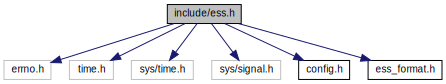
\includegraphics[width=350pt]{d1/d23/ess_8h__incl}
\end{center}
\end{figure}
This graph shows which files directly or indirectly include this file\+:
\nopagebreak
\begin{figure}[H]
\begin{center}
\leavevmode
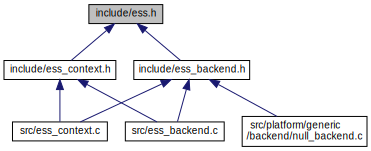
\includegraphics[width=350pt]{d6/de8/ess_8h__dep__incl}
\end{center}
\end{figure}
\subsection*{Macros}
\begin{DoxyCompactItemize}
\item 
\#define \hyperlink{ess_8h_a9091aabfdb114535c1058a3b62f5411b}{O\+P\+E\+N\+\_\+\+E\+S\+S\+\_\+\+V\+E\+R\+S\+I\+O\+N\+\_\+0\+\_\+5}
\end{DoxyCompactItemize}


\subsection{Detailed Description}
\begin{DoxyAuthor}{Author}
Anna Sopdia Schröck 
\end{DoxyAuthor}
\begin{DoxyDate}{Date}
2 Februar 20119 
\end{DoxyDate}


\subsection{Macro Definition Documentation}
\mbox{\Hypertarget{ess_8h_a9091aabfdb114535c1058a3b62f5411b}\label{ess_8h_a9091aabfdb114535c1058a3b62f5411b}} 
\index{ess.\+h@{ess.\+h}!O\+P\+E\+N\+\_\+\+E\+S\+S\+\_\+\+V\+E\+R\+S\+I\+O\+N\+\_\+0\+\_\+5@{O\+P\+E\+N\+\_\+\+E\+S\+S\+\_\+\+V\+E\+R\+S\+I\+O\+N\+\_\+0\+\_\+5}}
\index{O\+P\+E\+N\+\_\+\+E\+S\+S\+\_\+\+V\+E\+R\+S\+I\+O\+N\+\_\+0\+\_\+5@{O\+P\+E\+N\+\_\+\+E\+S\+S\+\_\+\+V\+E\+R\+S\+I\+O\+N\+\_\+0\+\_\+5}!ess.\+h@{ess.\+h}}
\subsubsection{\texorpdfstring{O\+P\+E\+N\+\_\+\+E\+S\+S\+\_\+\+V\+E\+R\+S\+I\+O\+N\+\_\+0\+\_\+5}{OPEN\_ESS\_VERSION\_0\_5}}
{\footnotesize\ttfamily \#define O\+P\+E\+N\+\_\+\+E\+S\+S\+\_\+\+V\+E\+R\+S\+I\+O\+N\+\_\+0\+\_\+5}



Definition at line 28 of file ess.\+h.


\hypertarget{ess__backend_8h}{}\section{include/ess\+\_\+backend.h File Reference}
\label{ess__backend_8h}\index{include/ess\+\_\+backend.\+h@{include/ess\+\_\+backend.\+h}}
{\ttfamily \#include \char`\"{}ess.\+h\char`\"{}}\newline
Include dependency graph for ess\+\_\+backend.\+h\+:\nopagebreak
\begin{figure}[H]
\begin{center}
\leavevmode
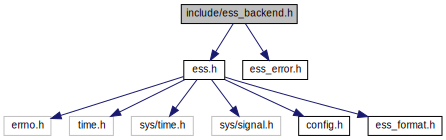
\includegraphics[width=224pt]{d0/df2/ess__backend_8h__incl}
\end{center}
\end{figure}
This graph shows which files directly or indirectly include this file\+:\nopagebreak
\begin{figure}[H]
\begin{center}
\leavevmode
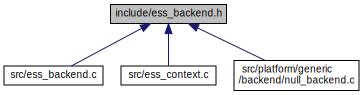
\includegraphics[width=350pt]{d2/df2/ess__backend_8h__dep__incl}
\end{center}
\end{figure}
\subsection*{Data Structures}
\begin{DoxyCompactItemize}
\item 
struct \hyperlink{structess__backend}{ess\+\_\+backend}
\begin{DoxyCompactList}\small\item\em ess backend factory \end{DoxyCompactList}\end{DoxyCompactItemize}
\subsection*{Typedefs}
\begin{DoxyCompactItemize}
\item 
typedef enum \hyperlink{ess__backend_8h_aac7bdeadfb36709a6f5ab36dda98fb72}{ess\+\_\+backend\+\_\+error} \hyperlink{ess__backend_8h_aa3de0496a3f361a6b38684e9cb65f01c}{ess\+\_\+backend\+\_\+error\+\_\+t}
\begin{DoxyCompactList}\small\item\em Audio backends error. \end{DoxyCompactList}\item 
typedef struct \hyperlink{structess__backend}{ess\+\_\+backend} \hyperlink{ess__backend_8h_ab1487f8c501b38b66796d0fbecb7ed7b}{ess\+\_\+backend\+\_\+facktory\+\_\+t}
\begin{DoxyCompactList}\small\item\em ess backend factory \end{DoxyCompactList}\end{DoxyCompactItemize}
\subsection*{Enumerations}
\begin{DoxyCompactItemize}
\item 
enum \hyperlink{ess__backend_8h_aac7bdeadfb36709a6f5ab36dda98fb72}{ess\+\_\+backend\+\_\+error} \{ \newline
\hyperlink{ess__backend_8h_aac7bdeadfb36709a6f5ab36dda98fb72a4abbaf43c0ba0a394549d3d5394e7545}{E\+S\+S\+\_\+\+B\+A\+C\+K\+E\+N\+D\+\_\+\+OK} = 0, 
\hyperlink{ess__backend_8h_aac7bdeadfb36709a6f5ab36dda98fb72a45ed0ae8199a02c26862792f30d35ebd}{E\+S\+S\+\_\+\+B\+A\+C\+K\+E\+N\+D\+\_\+\+O\+U\+T\+O\+F\+M\+EM} = -\/1, 
\hyperlink{ess__backend_8h_aac7bdeadfb36709a6f5ab36dda98fb72add38429c69b4419fb3ac6a66a6455834}{E\+S\+S\+\_\+\+B\+A\+C\+K\+E\+N\+D\+\_\+\+N\+O\+T\+\_\+\+F\+O\+U\+ND}, 
\hyperlink{ess__backend_8h_aac7bdeadfb36709a6f5ab36dda98fb72a1e60377ebbc9f5d7741aa3459fbf1f8d}{E\+S\+S\+\_\+\+B\+A\+C\+K\+E\+N\+D\+\_\+\+E\+R\+R\+O\+R\+\_\+\+W\+R\+O\+N\+G\+\_\+\+F\+O\+R\+M\+AT}, 
\newline
\hyperlink{ess__backend_8h_aac7bdeadfb36709a6f5ab36dda98fb72a073e5090b0053c3db2662c79aec5de76}{E\+S\+S\+\_\+\+B\+A\+C\+K\+E\+N\+D\+\_\+\+P\+A\+U\+S\+ED}, 
\hyperlink{ess__backend_8h_aac7bdeadfb36709a6f5ab36dda98fb72aec1740308fb5c8dbd28e701365024bf9}{E\+S\+S\+\_\+\+B\+A\+C\+K\+E\+N\+D\+\_\+\+E\+R\+R\+O\+R\+\_\+\+N\+U\+LL}, 
\hyperlink{ess__backend_8h_aac7bdeadfb36709a6f5ab36dda98fb72a1575cc2ec75e5e0912e283a5a8cad77c}{E\+S\+S\+\_\+\+B\+A\+C\+K\+E\+N\+D\+\_\+\+E\+R\+R\+OR}
 \}\begin{DoxyCompactList}\small\item\em Audio backends error. \end{DoxyCompactList}
\end{DoxyCompactItemize}
\subsection*{Functions}
\begin{DoxyCompactItemize}
\item 
int \hyperlink{ess__backend_8h_a6ba1bf553b596dd14d47748bec40bc9c}{ess\+\_\+backend\+\_\+get\+\_\+size} ()
\begin{DoxyCompactList}\small\item\em get the size of using backends \end{DoxyCompactList}\item 
\hyperlink{ess__backend_8h_ab1487f8c501b38b66796d0fbecb7ed7b}{ess\+\_\+backend\+\_\+facktory\+\_\+t} $\ast$ \hyperlink{ess__backend_8h_a16cb59b090351d9b9989de80b8bad520}{ess\+\_\+backend\+\_\+create\+\_\+factory\+\_\+list} ()
\item 
\hyperlink{ess__backend_8h_aa3de0496a3f361a6b38684e9cb65f01c}{ess\+\_\+backend\+\_\+error\+\_\+t} \hyperlink{ess__backend_8h_ab6129a1d1c11f81718f9122facfddd35}{ess\+\_\+backend\+\_\+destroy\+\_\+factory\+\_\+list} (\hyperlink{ess__backend_8h_ab1487f8c501b38b66796d0fbecb7ed7b}{ess\+\_\+backend\+\_\+facktory\+\_\+t} $\ast$list)
\item 
\hyperlink{ess__backend_8h_aa3de0496a3f361a6b38684e9cb65f01c}{ess\+\_\+backend\+\_\+error\+\_\+t} \hyperlink{ess__backend_8h_ae425d7c64cceee74831168327d858fed}{ess\+\_\+backend\+\_\+probe\+\_\+all} (const \hyperlink{ess__format_8h_ab03f24cb5d42f4448f713bf1ec178163}{ess\+\_\+format\+\_\+t} format, \hyperlink{ess__backend_8h_ab1487f8c501b38b66796d0fbecb7ed7b}{ess\+\_\+backend\+\_\+facktory\+\_\+t} $\ast$$\ast$backend)
\begin{DoxyCompactList}\small\item\em Check that all backends support the specified format and return all working backends. \end{DoxyCompactList}\item 
\hyperlink{ess__backend_8h_aa3de0496a3f361a6b38684e9cb65f01c}{ess\+\_\+backend\+\_\+error\+\_\+t} \hyperlink{ess__backend_8h_a9da07e785f1062832e5b0eadae2fd1b1}{ess\+\_\+backend\+\_\+probe} (const char $\ast$name, const \hyperlink{ess__format_8h_ab03f24cb5d42f4448f713bf1ec178163}{ess\+\_\+format\+\_\+t} format, \hyperlink{ess__backend_8h_ab1487f8c501b38b66796d0fbecb7ed7b}{ess\+\_\+backend\+\_\+facktory\+\_\+t} $\ast$backend)
\begin{DoxyCompactList}\small\item\em checked the backend with the specified name and returns it if successful. \end{DoxyCompactList}\item 
\hyperlink{ess__backend_8h_aa3de0496a3f361a6b38684e9cb65f01c}{ess\+\_\+backend\+\_\+error\+\_\+t} \hyperlink{ess__backend_8h_ab9b737a43ebfa9d220c02a32e79346d8}{ess\+\_\+backend\+\_\+set\+\_\+sample\+\_\+format} (\hyperlink{ess__backend_8h_ab1487f8c501b38b66796d0fbecb7ed7b}{ess\+\_\+backend\+\_\+facktory\+\_\+t} $\ast$backend, const \hyperlink{ess__format_8h_ab03f24cb5d42f4448f713bf1ec178163}{ess\+\_\+format\+\_\+t} forma)
\begin{DoxyCompactList}\small\item\em set sample format \end{DoxyCompactList}\item 
void $\ast$ \hyperlink{ess__backend_8h_a5adbfcb9ef73a620c893f59771c3f5e9}{ess\+\_\+backend\+\_\+get\+\_\+user\+\_\+daten} (\hyperlink{ess__backend_8h_ab1487f8c501b38b66796d0fbecb7ed7b}{ess\+\_\+backend\+\_\+facktory\+\_\+t} $\ast$backend)
\begin{DoxyCompactList}\small\item\em get user daten from backend (internal user) \end{DoxyCompactList}\item 
\hyperlink{ess__backend_8h_aa3de0496a3f361a6b38684e9cb65f01c}{ess\+\_\+backend\+\_\+error\+\_\+t} \hyperlink{ess__backend_8h_a6c9175335019d29a98371a855895a429}{ess\+\_\+backend\+\_\+set\+\_\+user\+\_\+daten} (\hyperlink{ess__backend_8h_ab1487f8c501b38b66796d0fbecb7ed7b}{ess\+\_\+backend\+\_\+facktory\+\_\+t} $\ast$backend, void $\ast$data)
\begin{DoxyCompactList}\small\item\em set user daten from backend (internal user) \end{DoxyCompactList}\end{DoxyCompactItemize}


\subsection{Typedef Documentation}
\mbox{\Hypertarget{ess__backend_8h_aa3de0496a3f361a6b38684e9cb65f01c}\label{ess__backend_8h_aa3de0496a3f361a6b38684e9cb65f01c}} 
\index{ess\+\_\+backend.\+h@{ess\+\_\+backend.\+h}!ess\+\_\+backend\+\_\+error\+\_\+t@{ess\+\_\+backend\+\_\+error\+\_\+t}}
\index{ess\+\_\+backend\+\_\+error\+\_\+t@{ess\+\_\+backend\+\_\+error\+\_\+t}!ess\+\_\+backend.\+h@{ess\+\_\+backend.\+h}}
\subsubsection{\texorpdfstring{ess\+\_\+backend\+\_\+error\+\_\+t}{ess\_backend\_error\_t}}
{\footnotesize\ttfamily typedef enum \hyperlink{ess__backend_8h_aac7bdeadfb36709a6f5ab36dda98fb72}{ess\+\_\+backend\+\_\+error}  \hyperlink{ess__backend_8h_aa3de0496a3f361a6b38684e9cb65f01c}{ess\+\_\+backend\+\_\+error\+\_\+t}}



Audio backends error. 

Error codes for the backend \mbox{\Hypertarget{ess__backend_8h_ab1487f8c501b38b66796d0fbecb7ed7b}\label{ess__backend_8h_ab1487f8c501b38b66796d0fbecb7ed7b}} 
\index{ess\+\_\+backend.\+h@{ess\+\_\+backend.\+h}!ess\+\_\+backend\+\_\+facktory\+\_\+t@{ess\+\_\+backend\+\_\+facktory\+\_\+t}}
\index{ess\+\_\+backend\+\_\+facktory\+\_\+t@{ess\+\_\+backend\+\_\+facktory\+\_\+t}!ess\+\_\+backend.\+h@{ess\+\_\+backend.\+h}}
\subsubsection{\texorpdfstring{ess\+\_\+backend\+\_\+facktory\+\_\+t}{ess\_backend\_facktory\_t}}
{\footnotesize\ttfamily typedef struct \hyperlink{structess__backend}{ess\+\_\+backend}  \hyperlink{ess__backend_8h_ab1487f8c501b38b66796d0fbecb7ed7b}{ess\+\_\+backend\+\_\+facktory\+\_\+t}}



ess backend factory 

Embedded Sound System Backend factory. Backend vtable 

\subsection{Enumeration Type Documentation}
\mbox{\Hypertarget{ess__backend_8h_aac7bdeadfb36709a6f5ab36dda98fb72}\label{ess__backend_8h_aac7bdeadfb36709a6f5ab36dda98fb72}} 
\index{ess\+\_\+backend.\+h@{ess\+\_\+backend.\+h}!ess\+\_\+backend\+\_\+error@{ess\+\_\+backend\+\_\+error}}
\index{ess\+\_\+backend\+\_\+error@{ess\+\_\+backend\+\_\+error}!ess\+\_\+backend.\+h@{ess\+\_\+backend.\+h}}
\subsubsection{\texorpdfstring{ess\+\_\+backend\+\_\+error}{ess\_backend\_error}}
{\footnotesize\ttfamily enum \hyperlink{ess__backend_8h_aac7bdeadfb36709a6f5ab36dda98fb72}{ess\+\_\+backend\+\_\+error}}



Audio backends error. 

Error codes for the backend \begin{DoxyEnumFields}{Enumerator}
\raisebox{\heightof{T}}[0pt][0pt]{\index{E\+S\+S\+\_\+\+B\+A\+C\+K\+E\+N\+D\+\_\+\+OK@{E\+S\+S\+\_\+\+B\+A\+C\+K\+E\+N\+D\+\_\+\+OK}!ess\+\_\+backend.\+h@{ess\+\_\+backend.\+h}}\index{ess\+\_\+backend.\+h@{ess\+\_\+backend.\+h}!E\+S\+S\+\_\+\+B\+A\+C\+K\+E\+N\+D\+\_\+\+OK@{E\+S\+S\+\_\+\+B\+A\+C\+K\+E\+N\+D\+\_\+\+OK}}}\mbox{\Hypertarget{ess__backend_8h_aac7bdeadfb36709a6f5ab36dda98fb72a4abbaf43c0ba0a394549d3d5394e7545}\label{ess__backend_8h_aac7bdeadfb36709a6f5ab36dda98fb72a4abbaf43c0ba0a394549d3d5394e7545}} 
E\+S\+S\+\_\+\+B\+A\+C\+K\+E\+N\+D\+\_\+\+OK&mo error. \\
\hline

\raisebox{\heightof{T}}[0pt][0pt]{\index{E\+S\+S\+\_\+\+B\+A\+C\+K\+E\+N\+D\+\_\+\+O\+U\+T\+O\+F\+M\+EM@{E\+S\+S\+\_\+\+B\+A\+C\+K\+E\+N\+D\+\_\+\+O\+U\+T\+O\+F\+M\+EM}!ess\+\_\+backend.\+h@{ess\+\_\+backend.\+h}}\index{ess\+\_\+backend.\+h@{ess\+\_\+backend.\+h}!E\+S\+S\+\_\+\+B\+A\+C\+K\+E\+N\+D\+\_\+\+O\+U\+T\+O\+F\+M\+EM@{E\+S\+S\+\_\+\+B\+A\+C\+K\+E\+N\+D\+\_\+\+O\+U\+T\+O\+F\+M\+EM}}}\mbox{\Hypertarget{ess__backend_8h_aac7bdeadfb36709a6f5ab36dda98fb72a45ed0ae8199a02c26862792f30d35ebd}\label{ess__backend_8h_aac7bdeadfb36709a6f5ab36dda98fb72a45ed0ae8199a02c26862792f30d35ebd}} 
E\+S\+S\+\_\+\+B\+A\+C\+K\+E\+N\+D\+\_\+\+O\+U\+T\+O\+F\+M\+EM&no more memory \\
\hline

\raisebox{\heightof{T}}[0pt][0pt]{\index{E\+S\+S\+\_\+\+B\+A\+C\+K\+E\+N\+D\+\_\+\+N\+O\+T\+\_\+\+F\+O\+U\+ND@{E\+S\+S\+\_\+\+B\+A\+C\+K\+E\+N\+D\+\_\+\+N\+O\+T\+\_\+\+F\+O\+U\+ND}!ess\+\_\+backend.\+h@{ess\+\_\+backend.\+h}}\index{ess\+\_\+backend.\+h@{ess\+\_\+backend.\+h}!E\+S\+S\+\_\+\+B\+A\+C\+K\+E\+N\+D\+\_\+\+N\+O\+T\+\_\+\+F\+O\+U\+ND@{E\+S\+S\+\_\+\+B\+A\+C\+K\+E\+N\+D\+\_\+\+N\+O\+T\+\_\+\+F\+O\+U\+ND}}}\mbox{\Hypertarget{ess__backend_8h_aac7bdeadfb36709a6f5ab36dda98fb72add38429c69b4419fb3ac6a66a6455834}\label{ess__backend_8h_aac7bdeadfb36709a6f5ab36dda98fb72add38429c69b4419fb3ac6a66a6455834}} 
E\+S\+S\+\_\+\+B\+A\+C\+K\+E\+N\+D\+\_\+\+N\+O\+T\+\_\+\+F\+O\+U\+ND&hardware for backend not avaible \\
\hline

\raisebox{\heightof{T}}[0pt][0pt]{\index{E\+S\+S\+\_\+\+B\+A\+C\+K\+E\+N\+D\+\_\+\+E\+R\+R\+O\+R\+\_\+\+W\+R\+O\+N\+G\+\_\+\+F\+O\+R\+M\+AT@{E\+S\+S\+\_\+\+B\+A\+C\+K\+E\+N\+D\+\_\+\+E\+R\+R\+O\+R\+\_\+\+W\+R\+O\+N\+G\+\_\+\+F\+O\+R\+M\+AT}!ess\+\_\+backend.\+h@{ess\+\_\+backend.\+h}}\index{ess\+\_\+backend.\+h@{ess\+\_\+backend.\+h}!E\+S\+S\+\_\+\+B\+A\+C\+K\+E\+N\+D\+\_\+\+E\+R\+R\+O\+R\+\_\+\+W\+R\+O\+N\+G\+\_\+\+F\+O\+R\+M\+AT@{E\+S\+S\+\_\+\+B\+A\+C\+K\+E\+N\+D\+\_\+\+E\+R\+R\+O\+R\+\_\+\+W\+R\+O\+N\+G\+\_\+\+F\+O\+R\+M\+AT}}}\mbox{\Hypertarget{ess__backend_8h_aac7bdeadfb36709a6f5ab36dda98fb72a1e60377ebbc9f5d7741aa3459fbf1f8d}\label{ess__backend_8h_aac7bdeadfb36709a6f5ab36dda98fb72a1e60377ebbc9f5d7741aa3459fbf1f8d}} 
E\+S\+S\+\_\+\+B\+A\+C\+K\+E\+N\+D\+\_\+\+E\+R\+R\+O\+R\+\_\+\+W\+R\+O\+N\+G\+\_\+\+F\+O\+R\+M\+AT&The format is not supported \\
\hline

\raisebox{\heightof{T}}[0pt][0pt]{\index{E\+S\+S\+\_\+\+B\+A\+C\+K\+E\+N\+D\+\_\+\+P\+A\+U\+S\+ED@{E\+S\+S\+\_\+\+B\+A\+C\+K\+E\+N\+D\+\_\+\+P\+A\+U\+S\+ED}!ess\+\_\+backend.\+h@{ess\+\_\+backend.\+h}}\index{ess\+\_\+backend.\+h@{ess\+\_\+backend.\+h}!E\+S\+S\+\_\+\+B\+A\+C\+K\+E\+N\+D\+\_\+\+P\+A\+U\+S\+ED@{E\+S\+S\+\_\+\+B\+A\+C\+K\+E\+N\+D\+\_\+\+P\+A\+U\+S\+ED}}}\mbox{\Hypertarget{ess__backend_8h_aac7bdeadfb36709a6f5ab36dda98fb72a073e5090b0053c3db2662c79aec5de76}\label{ess__backend_8h_aac7bdeadfb36709a6f5ab36dda98fb72a073e5090b0053c3db2662c79aec5de76}} 
E\+S\+S\+\_\+\+B\+A\+C\+K\+E\+N\+D\+\_\+\+P\+A\+U\+S\+ED&Don\textquotesingle{}t read or write becourse backend is paused \\
\hline

\raisebox{\heightof{T}}[0pt][0pt]{\index{E\+S\+S\+\_\+\+B\+A\+C\+K\+E\+N\+D\+\_\+\+E\+R\+R\+O\+R\+\_\+\+N\+U\+LL@{E\+S\+S\+\_\+\+B\+A\+C\+K\+E\+N\+D\+\_\+\+E\+R\+R\+O\+R\+\_\+\+N\+U\+LL}!ess\+\_\+backend.\+h@{ess\+\_\+backend.\+h}}\index{ess\+\_\+backend.\+h@{ess\+\_\+backend.\+h}!E\+S\+S\+\_\+\+B\+A\+C\+K\+E\+N\+D\+\_\+\+E\+R\+R\+O\+R\+\_\+\+N\+U\+LL@{E\+S\+S\+\_\+\+B\+A\+C\+K\+E\+N\+D\+\_\+\+E\+R\+R\+O\+R\+\_\+\+N\+U\+LL}}}\mbox{\Hypertarget{ess__backend_8h_aac7bdeadfb36709a6f5ab36dda98fb72aec1740308fb5c8dbd28e701365024bf9}\label{ess__backend_8h_aac7bdeadfb36709a6f5ab36dda98fb72aec1740308fb5c8dbd28e701365024bf9}} 
E\+S\+S\+\_\+\+B\+A\+C\+K\+E\+N\+D\+\_\+\+E\+R\+R\+O\+R\+\_\+\+N\+U\+LL&backend is null \\
\hline

\raisebox{\heightof{T}}[0pt][0pt]{\index{E\+S\+S\+\_\+\+B\+A\+C\+K\+E\+N\+D\+\_\+\+E\+R\+R\+OR@{E\+S\+S\+\_\+\+B\+A\+C\+K\+E\+N\+D\+\_\+\+E\+R\+R\+OR}!ess\+\_\+backend.\+h@{ess\+\_\+backend.\+h}}\index{ess\+\_\+backend.\+h@{ess\+\_\+backend.\+h}!E\+S\+S\+\_\+\+B\+A\+C\+K\+E\+N\+D\+\_\+\+E\+R\+R\+OR@{E\+S\+S\+\_\+\+B\+A\+C\+K\+E\+N\+D\+\_\+\+E\+R\+R\+OR}}}\mbox{\Hypertarget{ess__backend_8h_aac7bdeadfb36709a6f5ab36dda98fb72a1575cc2ec75e5e0912e283a5a8cad77c}\label{ess__backend_8h_aac7bdeadfb36709a6f5ab36dda98fb72a1575cc2ec75e5e0912e283a5a8cad77c}} 
E\+S\+S\+\_\+\+B\+A\+C\+K\+E\+N\+D\+\_\+\+E\+R\+R\+OR&unknown error \\
\hline

\end{DoxyEnumFields}


Definition at line 45 of file ess\+\_\+backend.\+h.


\begin{DoxyCode}
45                                \{
46   \hyperlink{ess__backend_8h_aac7bdeadfb36709a6f5ab36dda98fb72a4abbaf43c0ba0a394549d3d5394e7545}{ESS\_BACKEND\_OK} = 0,                 
47   \hyperlink{ess__backend_8h_aac7bdeadfb36709a6f5ab36dda98fb72a45ed0ae8199a02c26862792f30d35ebd}{ESS\_BACKEND\_OUTOFMEM} = -1,            
48   \hyperlink{ess__backend_8h_aac7bdeadfb36709a6f5ab36dda98fb72add38429c69b4419fb3ac6a66a6455834}{ESS\_BACKEND\_NOT\_FOUND},           
49   \hyperlink{ess__backend_8h_aac7bdeadfb36709a6f5ab36dda98fb72a1e60377ebbc9f5d7741aa3459fbf1f8d}{ESS\_BACKEND\_ERROR\_WRONG\_FORMAT},     
50   \hyperlink{ess__backend_8h_aac7bdeadfb36709a6f5ab36dda98fb72a073e5090b0053c3db2662c79aec5de76}{ESS\_BACKEND\_PAUSED},             
51   \hyperlink{ess__backend_8h_aac7bdeadfb36709a6f5ab36dda98fb72aec1740308fb5c8dbd28e701365024bf9}{ESS\_BACKEND\_ERROR\_NULL}, 
52   \hyperlink{ess__backend_8h_aac7bdeadfb36709a6f5ab36dda98fb72a1575cc2ec75e5e0912e283a5a8cad77c}{ESS\_BACKEND\_ERROR},               
53 \} \hyperlink{ess__backend_8h_aa3de0496a3f361a6b38684e9cb65f01c}{ess\_backend\_error\_t};
\end{DoxyCode}


\subsection{Function Documentation}
\mbox{\Hypertarget{ess__backend_8h_a16cb59b090351d9b9989de80b8bad520}\label{ess__backend_8h_a16cb59b090351d9b9989de80b8bad520}} 
\index{ess\+\_\+backend.\+h@{ess\+\_\+backend.\+h}!ess\+\_\+backend\+\_\+create\+\_\+factory\+\_\+list@{ess\+\_\+backend\+\_\+create\+\_\+factory\+\_\+list}}
\index{ess\+\_\+backend\+\_\+create\+\_\+factory\+\_\+list@{ess\+\_\+backend\+\_\+create\+\_\+factory\+\_\+list}!ess\+\_\+backend.\+h@{ess\+\_\+backend.\+h}}
\subsubsection{\texorpdfstring{ess\+\_\+backend\+\_\+create\+\_\+factory\+\_\+list()}{ess\_backend\_create\_factory\_list()}}
{\footnotesize\ttfamily \hyperlink{ess__backend_8h_ab1487f8c501b38b66796d0fbecb7ed7b}{ess\+\_\+backend\+\_\+facktory\+\_\+t}$\ast$ ess\+\_\+backend\+\_\+create\+\_\+factory\+\_\+list (\begin{DoxyParamCaption}{ }\end{DoxyParamCaption})}



Definition at line 44 of file ess\+\_\+backend.\+c.


\begin{DoxyCode}
44                                                           \{
45   \textcolor{keywordflow}{return} (\hyperlink{structess__backend}{ess\_backend\_facktory\_t}*)malloc(\textcolor{keyword}{sizeof}(
      \hyperlink{structess__backend}{ess\_backend\_facktory\_t}) * \hyperlink{ess__backend_8c_a6ba1bf553b596dd14d47748bec40bc9c}{ess\_backend\_get\_size}());
46 \}
\end{DoxyCode}
Here is the call graph for this function\+:\nopagebreak
\begin{figure}[H]
\begin{center}
\leavevmode
\includegraphics[width=339pt]{de/dc0/ess__backend_8h_a16cb59b090351d9b9989de80b8bad520_cgraph}
\end{center}
\end{figure}
\mbox{\Hypertarget{ess__backend_8h_ab6129a1d1c11f81718f9122facfddd35}\label{ess__backend_8h_ab6129a1d1c11f81718f9122facfddd35}} 
\index{ess\+\_\+backend.\+h@{ess\+\_\+backend.\+h}!ess\+\_\+backend\+\_\+destroy\+\_\+factory\+\_\+list@{ess\+\_\+backend\+\_\+destroy\+\_\+factory\+\_\+list}}
\index{ess\+\_\+backend\+\_\+destroy\+\_\+factory\+\_\+list@{ess\+\_\+backend\+\_\+destroy\+\_\+factory\+\_\+list}!ess\+\_\+backend.\+h@{ess\+\_\+backend.\+h}}
\subsubsection{\texorpdfstring{ess\+\_\+backend\+\_\+destroy\+\_\+factory\+\_\+list()}{ess\_backend\_destroy\_factory\_list()}}
{\footnotesize\ttfamily \hyperlink{ess__backend_8h_aa3de0496a3f361a6b38684e9cb65f01c}{ess\+\_\+backend\+\_\+error\+\_\+t} ess\+\_\+backend\+\_\+destroy\+\_\+factory\+\_\+list (\begin{DoxyParamCaption}\item[{\hyperlink{ess__backend_8h_ab1487f8c501b38b66796d0fbecb7ed7b}{ess\+\_\+backend\+\_\+facktory\+\_\+t} $\ast$}]{list }\end{DoxyParamCaption})}



Definition at line 47 of file ess\+\_\+backend.\+c.


\begin{DoxyCode}
47                                                                                    \{
48   \textcolor{keywordflow}{if}(list == 0)  \textcolor{keywordflow}{return} \hyperlink{ess__backend_8h_aac7bdeadfb36709a6f5ab36dda98fb72aec1740308fb5c8dbd28e701365024bf9}{ESS\_BACKEND\_ERROR\_NULL};
49   \textcolor{comment}{//free(list);}
50   \textcolor{keywordflow}{return} \hyperlink{ess__backend_8h_aac7bdeadfb36709a6f5ab36dda98fb72a4abbaf43c0ba0a394549d3d5394e7545}{ESS\_BACKEND\_OK};
51 \}
\end{DoxyCode}
\mbox{\Hypertarget{ess__backend_8h_a6ba1bf553b596dd14d47748bec40bc9c}\label{ess__backend_8h_a6ba1bf553b596dd14d47748bec40bc9c}} 
\index{ess\+\_\+backend.\+h@{ess\+\_\+backend.\+h}!ess\+\_\+backend\+\_\+get\+\_\+size@{ess\+\_\+backend\+\_\+get\+\_\+size}}
\index{ess\+\_\+backend\+\_\+get\+\_\+size@{ess\+\_\+backend\+\_\+get\+\_\+size}!ess\+\_\+backend.\+h@{ess\+\_\+backend.\+h}}
\subsubsection{\texorpdfstring{ess\+\_\+backend\+\_\+get\+\_\+size()}{ess\_backend\_get\_size()}}
{\footnotesize\ttfamily int ess\+\_\+backend\+\_\+get\+\_\+size (\begin{DoxyParamCaption}{ }\end{DoxyParamCaption})}



get the size of using backends 

\begin{DoxyReturn}{Returns}
number of support backends 
\end{DoxyReturn}


Definition at line 41 of file ess\+\_\+backend.\+c.


\begin{DoxyCode}
41                            \{
42   \textcolor{keywordflow}{return} \textcolor{keyword}{sizeof}(\hyperlink{ess__platform__esp32_8h_a0aae1a44ffbe4df0c0b4d13810ec8e22}{backends\_list}) / \textcolor{keyword}{sizeof}(\hyperlink{structess__backends__entry}{ess\_backends\_entry\_t});
43 \}
\end{DoxyCode}
Here is the caller graph for this function\+:\nopagebreak
\begin{figure}[H]
\begin{center}
\leavevmode
\includegraphics[width=350pt]{de/dc0/ess__backend_8h_a6ba1bf553b596dd14d47748bec40bc9c_icgraph}
\end{center}
\end{figure}
\mbox{\Hypertarget{ess__backend_8h_a5adbfcb9ef73a620c893f59771c3f5e9}\label{ess__backend_8h_a5adbfcb9ef73a620c893f59771c3f5e9}} 
\index{ess\+\_\+backend.\+h@{ess\+\_\+backend.\+h}!ess\+\_\+backend\+\_\+get\+\_\+user\+\_\+daten@{ess\+\_\+backend\+\_\+get\+\_\+user\+\_\+daten}}
\index{ess\+\_\+backend\+\_\+get\+\_\+user\+\_\+daten@{ess\+\_\+backend\+\_\+get\+\_\+user\+\_\+daten}!ess\+\_\+backend.\+h@{ess\+\_\+backend.\+h}}
\subsubsection{\texorpdfstring{ess\+\_\+backend\+\_\+get\+\_\+user\+\_\+daten()}{ess\_backend\_get\_user\_daten()}}
{\footnotesize\ttfamily void$\ast$ ess\+\_\+backend\+\_\+get\+\_\+user\+\_\+daten (\begin{DoxyParamCaption}\item[{\hyperlink{ess__backend_8h_ab1487f8c501b38b66796d0fbecb7ed7b}{ess\+\_\+backend\+\_\+facktory\+\_\+t} $\ast$}]{backend }\end{DoxyParamCaption})}



get user daten from backend (internal user) 


\begin{DoxyParams}[1]{Parameters}
\mbox{\tt in}  & {\em the} & using backend \\
\hline
\end{DoxyParams}
\begin{DoxyReturn}{Returns}
the user daten 
\end{DoxyReturn}


Definition at line 93 of file ess\+\_\+backend.\+c.


\begin{DoxyCode}
93                                                                   \{
94   \textcolor{keywordflow}{if}(backend == 0)  \textcolor{keywordflow}{return} 0;
95   \textcolor{keywordflow}{return}  backend->\hyperlink{structess__backend_a5ad8569143b4728c7b7f91c53661d8b5}{user\_daten};
96 \}
\end{DoxyCode}
\mbox{\Hypertarget{ess__backend_8h_a9da07e785f1062832e5b0eadae2fd1b1}\label{ess__backend_8h_a9da07e785f1062832e5b0eadae2fd1b1}} 
\index{ess\+\_\+backend.\+h@{ess\+\_\+backend.\+h}!ess\+\_\+backend\+\_\+probe@{ess\+\_\+backend\+\_\+probe}}
\index{ess\+\_\+backend\+\_\+probe@{ess\+\_\+backend\+\_\+probe}!ess\+\_\+backend.\+h@{ess\+\_\+backend.\+h}}
\subsubsection{\texorpdfstring{ess\+\_\+backend\+\_\+probe()}{ess\_backend\_probe()}}
{\footnotesize\ttfamily \hyperlink{ess__backend_8h_aa3de0496a3f361a6b38684e9cb65f01c}{ess\+\_\+backend\+\_\+error\+\_\+t} ess\+\_\+backend\+\_\+probe (\begin{DoxyParamCaption}\item[{const char $\ast$}]{name,  }\item[{const \hyperlink{ess__format_8h_ab03f24cb5d42f4448f713bf1ec178163}{ess\+\_\+format\+\_\+t}}]{format,  }\item[{\hyperlink{ess__backend_8h_ab1487f8c501b38b66796d0fbecb7ed7b}{ess\+\_\+backend\+\_\+facktory\+\_\+t} $\ast$}]{backend }\end{DoxyParamCaption})}



checked the backend with the specified name and returns it if successful. 


\begin{DoxyParams}{Parameters}
{\em Name} & of the backend \\
\hline
{\em format} & the format to probe \\
\hline
{\em backend} & return the working backend. if not null \\
\hline
\end{DoxyParams}

\begin{DoxyRetVals}{Return values}
{\em E\+S\+S\+\_\+\+B\+A\+C\+K\+E\+N\+D\+\_\+\+OK} & if backend support \\
\hline
{\em E\+S\+S\+\_\+\+B\+A\+C\+K\+E\+N\+D\+\_\+\+E\+R\+R\+O\+R\+\_\+\+W\+R\+O\+N\+G\+\_\+\+F\+O\+R\+M\+AT} & \\
\hline
{\em E\+S\+S\+\_\+\+B\+A\+C\+K\+E\+N\+D\+\_\+\+E\+R\+R\+OR} & \\
\hline
\end{DoxyRetVals}


Definition at line 76 of file ess\+\_\+backend.\+c.


\begin{DoxyCode}
76                                                                                                            
         \{
77   \textcolor{keywordflow}{for}(\textcolor{keywordtype}{unsigned} \textcolor{keywordtype}{int} i = 0; i < \hyperlink{ess__backend_8c_a6ba1bf553b596dd14d47748bec40bc9c}{ess\_backend\_get\_size}(); i++ ) \{
78     \textcolor{keywordflow}{if}(strcmp(\hyperlink{ess__platform__esp32_8h_a0aae1a44ffbe4df0c0b4d13810ec8e22}{backends\_list}[i].name, name)) \{
79       \textcolor{keywordflow}{if}(\hyperlink{ess__platform__esp32_8h_a0aae1a44ffbe4df0c0b4d13810ec8e22}{backends\_list}[i].getFactory()->ess\_backend\_probe(format)) \{
80         \textcolor{keywordflow}{if}(backend) backend = \hyperlink{ess__platform__esp32_8h_a0aae1a44ffbe4df0c0b4d13810ec8e22}{backends\_list}[i].\hyperlink{structess__backends__entry_a86f760dbdba11d491bc8209327d7e514}{getFactory}();
81         \textcolor{keywordflow}{return} \hyperlink{ess__backend_8h_aac7bdeadfb36709a6f5ab36dda98fb72a4abbaf43c0ba0a394549d3d5394e7545}{ESS\_BACKEND\_OK};
82       \} \textcolor{keywordflow}{else} \{
83         \textcolor{keywordflow}{return} \hyperlink{ess__backend_8h_aac7bdeadfb36709a6f5ab36dda98fb72a1e60377ebbc9f5d7741aa3459fbf1f8d}{ESS\_BACKEND\_ERROR\_WRONG\_FORMAT};
84       \}
85     \}
86   \}
87   \textcolor{keywordflow}{return} \hyperlink{ess__backend_8h_aac7bdeadfb36709a6f5ab36dda98fb72a1575cc2ec75e5e0912e283a5a8cad77c}{ESS\_BACKEND\_ERROR};
88 \}
\end{DoxyCode}
Here is the call graph for this function\+:\nopagebreak
\begin{figure}[H]
\begin{center}
\leavevmode
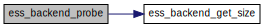
\includegraphics[width=336pt]{de/dc0/ess__backend_8h_a9da07e785f1062832e5b0eadae2fd1b1_cgraph}
\end{center}
\end{figure}
Here is the caller graph for this function\+:\nopagebreak
\begin{figure}[H]
\begin{center}
\leavevmode
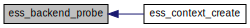
\includegraphics[width=308pt]{de/dc0/ess__backend_8h_a9da07e785f1062832e5b0eadae2fd1b1_icgraph}
\end{center}
\end{figure}
\mbox{\Hypertarget{ess__backend_8h_ae425d7c64cceee74831168327d858fed}\label{ess__backend_8h_ae425d7c64cceee74831168327d858fed}} 
\index{ess\+\_\+backend.\+h@{ess\+\_\+backend.\+h}!ess\+\_\+backend\+\_\+probe\+\_\+all@{ess\+\_\+backend\+\_\+probe\+\_\+all}}
\index{ess\+\_\+backend\+\_\+probe\+\_\+all@{ess\+\_\+backend\+\_\+probe\+\_\+all}!ess\+\_\+backend.\+h@{ess\+\_\+backend.\+h}}
\subsubsection{\texorpdfstring{ess\+\_\+backend\+\_\+probe\+\_\+all()}{ess\_backend\_probe\_all()}}
{\footnotesize\ttfamily \hyperlink{ess__backend_8h_aa3de0496a3f361a6b38684e9cb65f01c}{ess\+\_\+backend\+\_\+error\+\_\+t} ess\+\_\+backend\+\_\+probe\+\_\+all (\begin{DoxyParamCaption}\item[{const \hyperlink{ess__format_8h_ab03f24cb5d42f4448f713bf1ec178163}{ess\+\_\+format\+\_\+t}}]{format,  }\item[{\hyperlink{ess__backend_8h_ab1487f8c501b38b66796d0fbecb7ed7b}{ess\+\_\+backend\+\_\+facktory\+\_\+t} $\ast$$\ast$}]{backend }\end{DoxyParamCaption})}



Check that all backends support the specified format and return all working backends. 


\begin{DoxyParams}{Parameters}
{\em format} & the format to probe \\
\hline
{\em backend} & return all working backends. if not null \\
\hline
\end{DoxyParams}
\begin{DoxyReturn}{Returns}
number of working backends or errir codes 
\end{DoxyReturn}

\begin{DoxyRetVals}{Return values}
{\em E\+S\+S\+\_\+\+B\+A\+C\+K\+E\+N\+D\+\_\+\+E\+R\+R\+O\+R\+\_\+\+W\+R\+O\+N\+G\+\_\+\+F\+O\+R\+M\+AT} & when no backend supported \\
\hline
\end{DoxyRetVals}


Definition at line 52 of file ess\+\_\+backend.\+c.


\begin{DoxyCode}
52                                                                                                  \{
53   \hyperlink{structess__backend}{ess\_backend\_facktory\_t} *factory;
54 
55   \textcolor{keywordtype}{unsigned} \textcolor{keywordtype}{int} i,n = 0;
56 
57   \textcolor{keywordflow}{for}( i = 0; i < \hyperlink{ess__backend_8c_a6ba1bf553b596dd14d47748bec40bc9c}{ess\_backend\_get\_size}(); i++ ) \{
58     factory = \hyperlink{ess__platform__esp32_8h_a0aae1a44ffbe4df0c0b4d13810ec8e22}{backends\_list}[i].\hyperlink{structess__backends__entry_a86f760dbdba11d491bc8209327d7e514}{getFactory}();
59 
60     \textcolor{keywordflow}{if}(factory->\hyperlink{structess__backend_aae4f1015dadb3ed79975c5b7b78e547f}{ess\_backend\_probe}(format) != \hyperlink{ess__backend_8h_aac7bdeadfb36709a6f5ab36dda98fb72a4abbaf43c0ba0a394549d3d5394e7545}{ESS\_BACKEND\_OK}) \{
61       ESP\_LOGE(\hyperlink{ess__backend_8c_a7ce0df38eb467e59f209470c8f5ac4e6}{LOG\_TAG}, \textcolor{stringliteral}{"Failed to probe backend \(\backslash\)"%s\(\backslash\)""}, \hyperlink{ess__platform__esp32_8h_a0aae1a44ffbe4df0c0b4d13810ec8e22}{backends\_list}[i].name);
62       \textcolor{keywordflow}{continue};
63     \} \textcolor{keywordflow}{else} \{
64       ESP\_LOGI(\hyperlink{ess__backend_8c_a7ce0df38eb467e59f209470c8f5ac4e6}{LOG\_TAG},\textcolor{stringliteral}{"Possible format for backend: \(\backslash\)"%s\(\backslash\)" "}, 
      \hyperlink{ess__platform__esp32_8h_a0aae1a44ffbe4df0c0b4d13810ec8e22}{backends\_list}[i].name);
65       \textcolor{keywordflow}{if}(backend) \{ backend[n] = factory; \}
66       n++;
67     \}
68 
69   \}
70   ESP\_LOGI(\hyperlink{ess__backend_8c_a7ce0df38eb467e59f209470c8f5ac4e6}{LOG\_TAG},\textcolor{stringliteral}{"%d/%d backends probe possible\(\backslash\)n"}, n, 
      \hyperlink{ess__backend_8c_a6ba1bf553b596dd14d47748bec40bc9c}{ess\_backend\_get\_size}());
71 
72   \textcolor{keywordflow}{if}(n == 0) \textcolor{keywordflow}{return} \hyperlink{ess__backend_8h_aac7bdeadfb36709a6f5ab36dda98fb72a1e60377ebbc9f5d7741aa3459fbf1f8d}{ESS\_BACKEND\_ERROR\_WRONG\_FORMAT};
73   \textcolor{keywordflow}{return} n;
74 \}
\end{DoxyCode}
Here is the call graph for this function\+:\nopagebreak
\begin{figure}[H]
\begin{center}
\leavevmode
\includegraphics[width=350pt]{de/dc0/ess__backend_8h_ae425d7c64cceee74831168327d858fed_cgraph}
\end{center}
\end{figure}
\mbox{\Hypertarget{ess__backend_8h_ab9b737a43ebfa9d220c02a32e79346d8}\label{ess__backend_8h_ab9b737a43ebfa9d220c02a32e79346d8}} 
\index{ess\+\_\+backend.\+h@{ess\+\_\+backend.\+h}!ess\+\_\+backend\+\_\+set\+\_\+sample\+\_\+format@{ess\+\_\+backend\+\_\+set\+\_\+sample\+\_\+format}}
\index{ess\+\_\+backend\+\_\+set\+\_\+sample\+\_\+format@{ess\+\_\+backend\+\_\+set\+\_\+sample\+\_\+format}!ess\+\_\+backend.\+h@{ess\+\_\+backend.\+h}}
\subsubsection{\texorpdfstring{ess\+\_\+backend\+\_\+set\+\_\+sample\+\_\+format()}{ess\_backend\_set\_sample\_format()}}
{\footnotesize\ttfamily \hyperlink{ess__backend_8h_aa3de0496a3f361a6b38684e9cb65f01c}{ess\+\_\+backend\+\_\+error\+\_\+t} ess\+\_\+backend\+\_\+set\+\_\+sample\+\_\+format (\begin{DoxyParamCaption}\item[{\hyperlink{ess__backend_8h_ab1487f8c501b38b66796d0fbecb7ed7b}{ess\+\_\+backend\+\_\+facktory\+\_\+t} $\ast$}]{backend,  }\item[{const \hyperlink{ess__format_8h_ab03f24cb5d42f4448f713bf1ec178163}{ess\+\_\+format\+\_\+t}}]{forma }\end{DoxyParamCaption})}



set sample format 


\begin{DoxyParams}[1]{Parameters}
\mbox{\tt in}  & {\em backend} & the usiing backend \\
\hline
\mbox{\tt in}  & {\em forma} & sample format \\
\hline
\end{DoxyParams}

\begin{DoxyRetVals}{Return values}
{\em E\+S\+S\+\_\+\+B\+A\+C\+K\+E\+N\+D\+\_\+\+OK} & if backend support \\
\hline
{\em E\+S\+S\+\_\+\+B\+A\+C\+K\+E\+N\+D\+\_\+\+E\+R\+R\+O\+R\+\_\+\+W\+R\+O\+N\+G\+\_\+\+F\+O\+R\+M\+AT} & \\
\hline
{\em E\+S\+S\+\_\+\+B\+A\+C\+K\+E\+N\+D\+\_\+\+E\+R\+R\+OR} & \\
\hline
\end{DoxyRetVals}


Definition at line 89 of file ess\+\_\+backend.\+c.


\begin{DoxyCode}
89                                                                                                         \{
90   \textcolor{keywordflow}{if}(backend == 0) \textcolor{keywordflow}{return} \hyperlink{ess__backend_8h_aac7bdeadfb36709a6f5ab36dda98fb72aec1740308fb5c8dbd28e701365024bf9}{ESS\_BACKEND\_ERROR\_NULL};
91   \textcolor{keywordflow}{return} backend->\hyperlink{structess__backend_af8790cbdeabfcdafa015466bdb552ac2}{ess\_backend\_set\_sample\_format}(forma);
92 \}
\end{DoxyCode}
Here is the caller graph for this function\+:\nopagebreak
\begin{figure}[H]
\begin{center}
\leavevmode
\includegraphics[width=350pt]{de/dc0/ess__backend_8h_ab9b737a43ebfa9d220c02a32e79346d8_icgraph}
\end{center}
\end{figure}
\mbox{\Hypertarget{ess__backend_8h_a6c9175335019d29a98371a855895a429}\label{ess__backend_8h_a6c9175335019d29a98371a855895a429}} 
\index{ess\+\_\+backend.\+h@{ess\+\_\+backend.\+h}!ess\+\_\+backend\+\_\+set\+\_\+user\+\_\+daten@{ess\+\_\+backend\+\_\+set\+\_\+user\+\_\+daten}}
\index{ess\+\_\+backend\+\_\+set\+\_\+user\+\_\+daten@{ess\+\_\+backend\+\_\+set\+\_\+user\+\_\+daten}!ess\+\_\+backend.\+h@{ess\+\_\+backend.\+h}}
\subsubsection{\texorpdfstring{ess\+\_\+backend\+\_\+set\+\_\+user\+\_\+daten()}{ess\_backend\_set\_user\_daten()}}
{\footnotesize\ttfamily \hyperlink{ess__backend_8h_aa3de0496a3f361a6b38684e9cb65f01c}{ess\+\_\+backend\+\_\+error\+\_\+t} ess\+\_\+backend\+\_\+set\+\_\+user\+\_\+daten (\begin{DoxyParamCaption}\item[{\hyperlink{ess__backend_8h_ab1487f8c501b38b66796d0fbecb7ed7b}{ess\+\_\+backend\+\_\+facktory\+\_\+t} $\ast$}]{backend,  }\item[{void $\ast$}]{data }\end{DoxyParamCaption})}



set user daten from backend (internal user) 


\begin{DoxyParams}[1]{Parameters}
\mbox{\tt in}  & {\em the} & usiing backend \\
\hline
\mbox{\tt in}  & {\em data} & the using data \\
\hline
\end{DoxyParams}

\begin{DoxyRetVals}{Return values}
{\em E\+S\+S\+\_\+\+B\+A\+C\+K\+E\+N\+D\+\_\+\+OK} & \\
\hline
{\em E\+S\+S\+\_\+\+B\+A\+C\+K\+E\+N\+D\+\_\+\+E\+R\+R\+O\+R\+\_\+\+N\+U\+LL} & backend null \\
\hline
\end{DoxyRetVals}


Definition at line 97 of file ess\+\_\+backend.\+c.


\begin{DoxyCode}
97                                                                                             \{
98   \textcolor{keywordflow}{if}(backend == 0)  \textcolor{keywordflow}{return} \hyperlink{ess__backend_8h_aac7bdeadfb36709a6f5ab36dda98fb72aec1740308fb5c8dbd28e701365024bf9}{ESS\_BACKEND\_ERROR\_NULL};
99   backend->\hyperlink{structess__backend_a5ad8569143b4728c7b7f91c53661d8b5}{user\_daten} = data;
100   \textcolor{keywordflow}{return} \hyperlink{ess__backend_8h_aac7bdeadfb36709a6f5ab36dda98fb72a4abbaf43c0ba0a394549d3d5394e7545}{ESS\_BACKEND\_OK};
101 \}
\end{DoxyCode}

\hypertarget{ess__context_8h}{}\section{include/ess\+\_\+context.h File Reference}
\label{ess__context_8h}\index{include/ess\+\_\+context.\+h@{include/ess\+\_\+context.\+h}}
{\ttfamily \#include \char`\"{}ess.\+h\char`\"{}}\newline
{\ttfamily \#include \char`\"{}ess\+\_\+format.\+h\char`\"{}}\newline
Include dependency graph for ess\+\_\+context.\+h\+:
\nopagebreak
\begin{figure}[H]
\begin{center}
\leavevmode
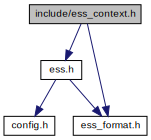
\includegraphics[width=224pt]{d8/d13/ess__context_8h__incl}
\end{center}
\end{figure}
This graph shows which files directly or indirectly include this file\+:
\nopagebreak
\begin{figure}[H]
\begin{center}
\leavevmode
\includegraphics[width=292pt]{d7/d03/ess__context_8h__dep__incl}
\end{center}
\end{figure}
\subsection*{Data Structures}
\begin{DoxyCompactItemize}
\item 
struct \hyperlink{structess__context}{ess\+\_\+context}
\begin{DoxyCompactList}\small\item\em ess context \end{DoxyCompactList}\end{DoxyCompactItemize}
\subsection*{Typedefs}
\begin{DoxyCompactItemize}
\item 
typedef struct \hyperlink{structess__backend}{ess\+\_\+backend} \hyperlink{ess__context_8h_aaf61f8f05f797647c229f2f8167c8e6e}{ess\+\_\+backend\+\_\+facktory\+\_\+t}
\item 
typedef enum \hyperlink{ess__context_8h_a55313861d12b8c596371cace86eacc2e}{ess\+\_\+context\+\_\+status} \hyperlink{ess__context_8h_adb5314cbbcb2bed6fc8b770d8ef3257c}{ess\+\_\+context\+\_\+status\+\_\+t}
\begin{DoxyCompactList}\small\item\em Audio context stats. \end{DoxyCompactList}\item 
typedef enum \hyperlink{ess__context_8h_a4b185bc84680674eb2efc8f720d3362b}{ess\+\_\+context\+\_\+error} \hyperlink{ess__context_8h_acc807999e4f53d1867abf8a0ac682f33}{ess\+\_\+context\+\_\+error\+\_\+t}
\begin{DoxyCompactList}\small\item\em ess context error codes \end{DoxyCompactList}\item 
typedef struct \hyperlink{structess__context}{ess\+\_\+context} \hyperlink{ess__context_8h_a8a8fec5766c0b3615f8f12f7948e949b}{ess\+\_\+context\+\_\+t}
\begin{DoxyCompactList}\small\item\em ess context \end{DoxyCompactList}\end{DoxyCompactItemize}
\subsection*{Enumerations}
\begin{DoxyCompactItemize}
\item 
enum \hyperlink{ess__context_8h_a55313861d12b8c596371cace86eacc2e}{ess\+\_\+context\+\_\+status} \{ \newline
\hyperlink{ess__context_8h_a55313861d12b8c596371cace86eacc2ea2ee2157354733689af9991d071d24d24}{E\+S\+S\+\_\+\+C\+O\+N\+T\+E\+X\+T\+\_\+\+S\+T\+A\+T\+U\+S\+\_\+\+C\+R\+E\+A\+T\+ED}, 
\hyperlink{ess__context_8h_a55313861d12b8c596371cace86eacc2eada32323ceb7303d5432781a25cef7f65}{E\+S\+S\+\_\+\+C\+O\+N\+T\+E\+X\+T\+\_\+\+S\+T\+A\+T\+U\+S\+\_\+\+R\+UN}, 
\hyperlink{ess__context_8h_a55313861d12b8c596371cace86eacc2ea6f6315ef32fd6f85789578726d3d06b9}{E\+S\+S\+\_\+\+C\+O\+N\+T\+E\+X\+T\+\_\+\+S\+T\+A\+T\+U\+S\+\_\+\+P\+A\+U\+S\+ED}, 
\hyperlink{ess__context_8h_a55313861d12b8c596371cace86eacc2ea6ca265da2cff09e1478d2bdf8d1ebe9b}{E\+S\+S\+\_\+\+C\+O\+N\+T\+E\+X\+T\+\_\+\+S\+T\+A\+T\+U\+S\+\_\+\+E\+R\+R\+OR}, 
\newline
\hyperlink{ess__context_8h_a55313861d12b8c596371cace86eacc2ea5941ca16a82f0818868363bd2c2fca57}{E\+S\+S\+\_\+\+C\+O\+N\+T\+E\+X\+T\+\_\+\+S\+T\+A\+T\+U\+S\+\_\+\+R\+E\+S\+T\+A\+RT}, 
\hyperlink{ess__context_8h_a55313861d12b8c596371cace86eacc2ea4dd76905722568e7e99af4ef39438662}{E\+S\+S\+\_\+\+C\+O\+N\+T\+E\+X\+T\+\_\+\+S\+T\+A\+T\+U\+S\+\_\+\+C\+L\+O\+SE}
 \}\begin{DoxyCompactList}\small\item\em Audio context stats. \end{DoxyCompactList}
\item 
enum \hyperlink{ess__context_8h_a4b185bc84680674eb2efc8f720d3362b}{ess\+\_\+context\+\_\+error} \{ \newline
\hyperlink{ess__context_8h_a4b185bc84680674eb2efc8f720d3362ba5fbe734224f5adb51e59c6dd88506d60}{E\+S\+S\+\_\+\+C\+O\+N\+T\+E\+X\+T\+\_\+\+E\+R\+R\+O\+R\+\_\+\+OK} = 0, 
\hyperlink{ess__context_8h_a4b185bc84680674eb2efc8f720d3362ba020750f30895b9adb7b2814810976de0}{E\+S\+S\+\_\+\+C\+O\+N\+T\+E\+X\+T\+\_\+\+E\+R\+R\+O\+R\+\_\+\+O\+U\+T\+O\+F\+M\+EM} = -\/1, 
\hyperlink{ess__context_8h_a4b185bc84680674eb2efc8f720d3362ba29dbe40f674348273f3b23c9c5fcf62d}{E\+S\+S\+\_\+\+C\+O\+N\+T\+E\+X\+T\+\_\+\+E\+R\+R\+O\+R\+N\+O\+B\+A\+C\+K\+E\+ND}, 
\hyperlink{ess__context_8h_a4b185bc84680674eb2efc8f720d3362bace646ce156ae1461491206d2bfa7f902}{E\+S\+S\+\_\+\+C\+O\+N\+T\+E\+X\+T\+\_\+\+W\+R\+O\+N\+G\+F\+O\+R\+M\+AT}, 
\newline
\hyperlink{ess__context_8h_a4b185bc84680674eb2efc8f720d3362baa6ed95d92bbe32c445b0adce2fc256ce}{E\+S\+S\+\_\+\+C\+O\+N\+T\+E\+X\+T\+\_\+\+E\+R\+R\+OR}, 
\hyperlink{ess__context_8h_a4b185bc84680674eb2efc8f720d3362baf33b77dd00f57d9dd7ab4909e3559dae}{E\+S\+S\+\_\+\+C\+O\+N\+T\+E\+X\+\_\+\+I\+S\+P\+A\+U\+S\+ED} = -\/42
 \}\begin{DoxyCompactList}\small\item\em ess context error codes \end{DoxyCompactList}
\end{DoxyCompactItemize}
\subsection*{Functions}
\begin{DoxyCompactItemize}
\item 
\hyperlink{ess__context_8h_acc807999e4f53d1867abf8a0ac682f33}{ess\+\_\+context\+\_\+error\+\_\+t} \hyperlink{ess__context_8h_ac764fbb6b72712d2b755f54c6b240e33}{ess\+\_\+context\+\_\+create} (\hyperlink{ess__context_8h_a8a8fec5766c0b3615f8f12f7948e949b}{ess\+\_\+context\+\_\+t} $\ast$context, const \hyperlink{ess__format_8h_ab03f24cb5d42f4448f713bf1ec178163}{ess\+\_\+format\+\_\+t} format)
\begin{DoxyCompactList}\small\item\em creater the context \end{DoxyCompactList}\item 
\hyperlink{ess__context_8h_acc807999e4f53d1867abf8a0ac682f33}{ess\+\_\+context\+\_\+error\+\_\+t} \hyperlink{ess__context_8h_a40a2211f2793b0346c879b61b35ff63e}{ess\+\_\+context\+\_\+init} (\hyperlink{ess__context_8h_a8a8fec5766c0b3615f8f12f7948e949b}{ess\+\_\+context\+\_\+t} $\ast$context, const char $\ast$name)
\begin{DoxyCompactList}\small\item\em initialisiert the context \end{DoxyCompactList}\item 
\hyperlink{ess__context_8h_acc807999e4f53d1867abf8a0ac682f33}{ess\+\_\+context\+\_\+error\+\_\+t} \hyperlink{ess__context_8h_a26ae0093adaa4a6945fed6cfd31d4ae7}{ess\+\_\+context\+\_\+init\+\_\+ex} (\hyperlink{ess__context_8h_a8a8fec5766c0b3615f8f12f7948e949b}{ess\+\_\+context\+\_\+t} $\ast$context, \hyperlink{ess__backend_8h_ab1487f8c501b38b66796d0fbecb7ed7b}{ess\+\_\+backend\+\_\+facktory\+\_\+t} $\ast$backend)
\begin{DoxyCompactList}\small\item\em initialisiert the context with a user backend \end{DoxyCompactList}\item 
\hyperlink{ess__context_8h_acc807999e4f53d1867abf8a0ac682f33}{ess\+\_\+context\+\_\+error\+\_\+t} \hyperlink{ess__context_8h_a9a12468e0f826cc92385be2df34a38d4}{ess\+\_\+context\+\_\+close} (\hyperlink{ess__context_8h_a8a8fec5766c0b3615f8f12f7948e949b}{ess\+\_\+context\+\_\+t} $\ast$context)
\begin{DoxyCompactList}\small\item\em close the context and close the backend \end{DoxyCompactList}\item 
\hyperlink{ess__context_8h_acc807999e4f53d1867abf8a0ac682f33}{ess\+\_\+context\+\_\+error\+\_\+t} \hyperlink{ess__context_8h_a0a9e96c03cba2bfef2999c0199070d17}{ess\+\_\+context\+\_\+destroy} (\hyperlink{ess__context_8h_a8a8fec5766c0b3615f8f12f7948e949b}{ess\+\_\+context\+\_\+t} $\ast$context)
\begin{DoxyCompactList}\small\item\em destroy and free the context \end{DoxyCompactList}\item 
\hyperlink{ess__context_8h_acc807999e4f53d1867abf8a0ac682f33}{ess\+\_\+context\+\_\+error\+\_\+t} \hyperlink{ess__context_8h_a6b450cd4cfd4fed931f99b05c38e0172}{ess\+\_\+context\+\_\+paused} (\hyperlink{ess__context_8h_a8a8fec5766c0b3615f8f12f7948e949b}{ess\+\_\+context\+\_\+t} $\ast$context)
\begin{DoxyCompactList}\small\item\em set backend to standby \end{DoxyCompactList}\item 
\hyperlink{ess__context_8h_acc807999e4f53d1867abf8a0ac682f33}{ess\+\_\+context\+\_\+error\+\_\+t} \hyperlink{ess__context_8h_ac6041313862e70f48b8441df8136b0ba}{ess\+\_\+context\+\_\+resume} (\hyperlink{ess__context_8h_a8a8fec5766c0b3615f8f12f7948e949b}{ess\+\_\+context\+\_\+t} $\ast$context)
\begin{DoxyCompactList}\small\item\em set backend to run \end{DoxyCompactList}\item 
\hyperlink{ess__context_8h_acc807999e4f53d1867abf8a0ac682f33}{ess\+\_\+context\+\_\+error\+\_\+t} \hyperlink{ess__context_8h_aebeaf3ec64fe0e348557884dfa601944}{ess\+\_\+context\+\_\+set\+\_\+format} (\hyperlink{ess__context_8h_a8a8fec5766c0b3615f8f12f7948e949b}{ess\+\_\+context\+\_\+t} $\ast$context, const \hyperlink{ess__format_8h_ab03f24cb5d42f4448f713bf1ec178163}{ess\+\_\+format\+\_\+t} format)
\begin{DoxyCompactList}\small\item\em set the sample format to backend \end{DoxyCompactList}\item 
unsigned int \hyperlink{ess__context_8h_ae2c6a4e2f8a5128fc1bb05afea5f3c8d}{ess\+\_\+context\+\_\+write} (\hyperlink{ess__context_8h_a8a8fec5766c0b3615f8f12f7948e949b}{ess\+\_\+context\+\_\+t} $\ast$context, void $\ast$buffer, unsigned int buf\+\_\+size)
\begin{DoxyCompactList}\small\item\em write audio data to the backend \end{DoxyCompactList}\item 
\hyperlink{ess__context_8h_acc807999e4f53d1867abf8a0ac682f33}{ess\+\_\+context\+\_\+error\+\_\+t} \hyperlink{ess__context_8h_a8077482da675241fd832152974033994}{ess\+\_\+context\+\_\+write\+\_\+ex} (\hyperlink{ess__context_8h_a8a8fec5766c0b3615f8f12f7948e949b}{ess\+\_\+context\+\_\+t} $\ast$context, void $\ast$buffer, unsigned int buf\+\_\+size, unsigned int $\ast$wrote)
\begin{DoxyCompactList}\small\item\em write audio data to the backend \end{DoxyCompactList}\item 
const char $\ast$ \hyperlink{ess__context_8h_a1038af3d90a5a8a45d4fc35cbd425e5b}{ess\+\_\+context\+\_\+get\+\_\+backend\+\_\+name} (\hyperlink{ess__context_8h_a8a8fec5766c0b3615f8f12f7948e949b}{ess\+\_\+context\+\_\+t} $\ast$context)
\begin{DoxyCompactList}\small\item\em get the usind backend name \end{DoxyCompactList}\item 
const char $\ast$ \hyperlink{ess__context_8h_a139494e2518952f79ec0bc7d788d7612}{ess\+\_\+context\+\_\+get\+\_\+backend\+\_\+info} (\hyperlink{ess__context_8h_a8a8fec5766c0b3615f8f12f7948e949b}{ess\+\_\+context\+\_\+t} $\ast$context)
\begin{DoxyCompactList}\small\item\em get using backend informations \end{DoxyCompactList}\item 
\hyperlink{ess__context_8h_acc807999e4f53d1867abf8a0ac682f33}{ess\+\_\+context\+\_\+error\+\_\+t} \hyperlink{ess__context_8h_ae8c078f30231eae2756ff85825dac90a}{ess\+\_\+context\+\_\+get\+\_\+last\+\_\+error} (\hyperlink{ess__context_8h_a8a8fec5766c0b3615f8f12f7948e949b}{ess\+\_\+context\+\_\+t} $\ast$context)
\begin{DoxyCompactList}\small\item\em get the last error from context \end{DoxyCompactList}\end{DoxyCompactItemize}


\subsection{Typedef Documentation}
\mbox{\Hypertarget{ess__context_8h_aaf61f8f05f797647c229f2f8167c8e6e}\label{ess__context_8h_aaf61f8f05f797647c229f2f8167c8e6e}} 
\index{ess\+\_\+context.\+h@{ess\+\_\+context.\+h}!ess\+\_\+backend\+\_\+facktory\+\_\+t@{ess\+\_\+backend\+\_\+facktory\+\_\+t}}
\index{ess\+\_\+backend\+\_\+facktory\+\_\+t@{ess\+\_\+backend\+\_\+facktory\+\_\+t}!ess\+\_\+context.\+h@{ess\+\_\+context.\+h}}
\subsubsection{\texorpdfstring{ess\+\_\+backend\+\_\+facktory\+\_\+t}{ess\_backend\_facktory\_t}}
{\footnotesize\ttfamily typedef struct \hyperlink{structess__backend}{ess\+\_\+backend} \hyperlink{ess__backend_8h_ab1487f8c501b38b66796d0fbecb7ed7b}{ess\+\_\+backend\+\_\+facktory\+\_\+t}}



Definition at line 40 of file ess\+\_\+context.\+h.

\mbox{\Hypertarget{ess__context_8h_acc807999e4f53d1867abf8a0ac682f33}\label{ess__context_8h_acc807999e4f53d1867abf8a0ac682f33}} 
\index{ess\+\_\+context.\+h@{ess\+\_\+context.\+h}!ess\+\_\+context\+\_\+error\+\_\+t@{ess\+\_\+context\+\_\+error\+\_\+t}}
\index{ess\+\_\+context\+\_\+error\+\_\+t@{ess\+\_\+context\+\_\+error\+\_\+t}!ess\+\_\+context.\+h@{ess\+\_\+context.\+h}}
\subsubsection{\texorpdfstring{ess\+\_\+context\+\_\+error\+\_\+t}{ess\_context\_error\_t}}
{\footnotesize\ttfamily typedef enum \hyperlink{ess__context_8h_a4b185bc84680674eb2efc8f720d3362b}{ess\+\_\+context\+\_\+error} \hyperlink{ess__context_8h_acc807999e4f53d1867abf8a0ac682f33}{ess\+\_\+context\+\_\+error\+\_\+t}}



ess context error codes 

\mbox{\Hypertarget{ess__context_8h_adb5314cbbcb2bed6fc8b770d8ef3257c}\label{ess__context_8h_adb5314cbbcb2bed6fc8b770d8ef3257c}} 
\index{ess\+\_\+context.\+h@{ess\+\_\+context.\+h}!ess\+\_\+context\+\_\+status\+\_\+t@{ess\+\_\+context\+\_\+status\+\_\+t}}
\index{ess\+\_\+context\+\_\+status\+\_\+t@{ess\+\_\+context\+\_\+status\+\_\+t}!ess\+\_\+context.\+h@{ess\+\_\+context.\+h}}
\subsubsection{\texorpdfstring{ess\+\_\+context\+\_\+status\+\_\+t}{ess\_context\_status\_t}}
{\footnotesize\ttfamily typedef enum \hyperlink{ess__context_8h_a55313861d12b8c596371cace86eacc2e}{ess\+\_\+context\+\_\+status}  \hyperlink{ess__context_8h_adb5314cbbcb2bed6fc8b770d8ef3257c}{ess\+\_\+context\+\_\+status\+\_\+t}}



Audio context stats. 

\mbox{\Hypertarget{ess__context_8h_a8a8fec5766c0b3615f8f12f7948e949b}\label{ess__context_8h_a8a8fec5766c0b3615f8f12f7948e949b}} 
\index{ess\+\_\+context.\+h@{ess\+\_\+context.\+h}!ess\+\_\+context\+\_\+t@{ess\+\_\+context\+\_\+t}}
\index{ess\+\_\+context\+\_\+t@{ess\+\_\+context\+\_\+t}!ess\+\_\+context.\+h@{ess\+\_\+context.\+h}}
\subsubsection{\texorpdfstring{ess\+\_\+context\+\_\+t}{ess\_context\_t}}
{\footnotesize\ttfamily typedef struct \hyperlink{structess__context}{ess\+\_\+context} \hyperlink{ess__context_8h_a8a8fec5766c0b3615f8f12f7948e949b}{ess\+\_\+context\+\_\+t}}



ess context 

Embedded sound server context. Abstract managment 

\subsection{Enumeration Type Documentation}
\mbox{\Hypertarget{ess__context_8h_a4b185bc84680674eb2efc8f720d3362b}\label{ess__context_8h_a4b185bc84680674eb2efc8f720d3362b}} 
\index{ess\+\_\+context.\+h@{ess\+\_\+context.\+h}!ess\+\_\+context\+\_\+error@{ess\+\_\+context\+\_\+error}}
\index{ess\+\_\+context\+\_\+error@{ess\+\_\+context\+\_\+error}!ess\+\_\+context.\+h@{ess\+\_\+context.\+h}}
\subsubsection{\texorpdfstring{ess\+\_\+context\+\_\+error}{ess\_context\_error}}
{\footnotesize\ttfamily enum \hyperlink{ess__context_8h_a4b185bc84680674eb2efc8f720d3362b}{ess\+\_\+context\+\_\+error}}



ess context error codes 

\begin{DoxyEnumFields}{Enumerator}
\raisebox{\heightof{T}}[0pt][0pt]{\index{E\+S\+S\+\_\+\+C\+O\+N\+T\+E\+X\+T\+\_\+\+E\+R\+R\+O\+R\+\_\+\+OK@{E\+S\+S\+\_\+\+C\+O\+N\+T\+E\+X\+T\+\_\+\+E\+R\+R\+O\+R\+\_\+\+OK}!ess\+\_\+context.\+h@{ess\+\_\+context.\+h}}\index{ess\+\_\+context.\+h@{ess\+\_\+context.\+h}!E\+S\+S\+\_\+\+C\+O\+N\+T\+E\+X\+T\+\_\+\+E\+R\+R\+O\+R\+\_\+\+OK@{E\+S\+S\+\_\+\+C\+O\+N\+T\+E\+X\+T\+\_\+\+E\+R\+R\+O\+R\+\_\+\+OK}}}\mbox{\Hypertarget{ess__context_8h_a4b185bc84680674eb2efc8f720d3362ba5fbe734224f5adb51e59c6dd88506d60}\label{ess__context_8h_a4b185bc84680674eb2efc8f720d3362ba5fbe734224f5adb51e59c6dd88506d60}} 
E\+S\+S\+\_\+\+C\+O\+N\+T\+E\+X\+T\+\_\+\+E\+R\+R\+O\+R\+\_\+\+OK&no error \\
\hline

\raisebox{\heightof{T}}[0pt][0pt]{\index{E\+S\+S\+\_\+\+C\+O\+N\+T\+E\+X\+T\+\_\+\+E\+R\+R\+O\+R\+\_\+\+O\+U\+T\+O\+F\+M\+EM@{E\+S\+S\+\_\+\+C\+O\+N\+T\+E\+X\+T\+\_\+\+E\+R\+R\+O\+R\+\_\+\+O\+U\+T\+O\+F\+M\+EM}!ess\+\_\+context.\+h@{ess\+\_\+context.\+h}}\index{ess\+\_\+context.\+h@{ess\+\_\+context.\+h}!E\+S\+S\+\_\+\+C\+O\+N\+T\+E\+X\+T\+\_\+\+E\+R\+R\+O\+R\+\_\+\+O\+U\+T\+O\+F\+M\+EM@{E\+S\+S\+\_\+\+C\+O\+N\+T\+E\+X\+T\+\_\+\+E\+R\+R\+O\+R\+\_\+\+O\+U\+T\+O\+F\+M\+EM}}}\mbox{\Hypertarget{ess__context_8h_a4b185bc84680674eb2efc8f720d3362ba020750f30895b9adb7b2814810976de0}\label{ess__context_8h_a4b185bc84680674eb2efc8f720d3362ba020750f30895b9adb7b2814810976de0}} 
E\+S\+S\+\_\+\+C\+O\+N\+T\+E\+X\+T\+\_\+\+E\+R\+R\+O\+R\+\_\+\+O\+U\+T\+O\+F\+M\+EM&out of memory \\
\hline

\raisebox{\heightof{T}}[0pt][0pt]{\index{E\+S\+S\+\_\+\+C\+O\+N\+T\+E\+X\+T\+\_\+\+E\+R\+R\+O\+R\+N\+O\+B\+A\+C\+K\+E\+ND@{E\+S\+S\+\_\+\+C\+O\+N\+T\+E\+X\+T\+\_\+\+E\+R\+R\+O\+R\+N\+O\+B\+A\+C\+K\+E\+ND}!ess\+\_\+context.\+h@{ess\+\_\+context.\+h}}\index{ess\+\_\+context.\+h@{ess\+\_\+context.\+h}!E\+S\+S\+\_\+\+C\+O\+N\+T\+E\+X\+T\+\_\+\+E\+R\+R\+O\+R\+N\+O\+B\+A\+C\+K\+E\+ND@{E\+S\+S\+\_\+\+C\+O\+N\+T\+E\+X\+T\+\_\+\+E\+R\+R\+O\+R\+N\+O\+B\+A\+C\+K\+E\+ND}}}\mbox{\Hypertarget{ess__context_8h_a4b185bc84680674eb2efc8f720d3362ba29dbe40f674348273f3b23c9c5fcf62d}\label{ess__context_8h_a4b185bc84680674eb2efc8f720d3362ba29dbe40f674348273f3b23c9c5fcf62d}} 
E\+S\+S\+\_\+\+C\+O\+N\+T\+E\+X\+T\+\_\+\+E\+R\+R\+O\+R\+N\+O\+B\+A\+C\+K\+E\+ND&context has no backend \\
\hline

\raisebox{\heightof{T}}[0pt][0pt]{\index{E\+S\+S\+\_\+\+C\+O\+N\+T\+E\+X\+T\+\_\+\+W\+R\+O\+N\+G\+F\+O\+R\+M\+AT@{E\+S\+S\+\_\+\+C\+O\+N\+T\+E\+X\+T\+\_\+\+W\+R\+O\+N\+G\+F\+O\+R\+M\+AT}!ess\+\_\+context.\+h@{ess\+\_\+context.\+h}}\index{ess\+\_\+context.\+h@{ess\+\_\+context.\+h}!E\+S\+S\+\_\+\+C\+O\+N\+T\+E\+X\+T\+\_\+\+W\+R\+O\+N\+G\+F\+O\+R\+M\+AT@{E\+S\+S\+\_\+\+C\+O\+N\+T\+E\+X\+T\+\_\+\+W\+R\+O\+N\+G\+F\+O\+R\+M\+AT}}}\mbox{\Hypertarget{ess__context_8h_a4b185bc84680674eb2efc8f720d3362bace646ce156ae1461491206d2bfa7f902}\label{ess__context_8h_a4b185bc84680674eb2efc8f720d3362bace646ce156ae1461491206d2bfa7f902}} 
E\+S\+S\+\_\+\+C\+O\+N\+T\+E\+X\+T\+\_\+\+W\+R\+O\+N\+G\+F\+O\+R\+M\+AT&context format is not supported from backend \\
\hline

\raisebox{\heightof{T}}[0pt][0pt]{\index{E\+S\+S\+\_\+\+C\+O\+N\+T\+E\+X\+T\+\_\+\+E\+R\+R\+OR@{E\+S\+S\+\_\+\+C\+O\+N\+T\+E\+X\+T\+\_\+\+E\+R\+R\+OR}!ess\+\_\+context.\+h@{ess\+\_\+context.\+h}}\index{ess\+\_\+context.\+h@{ess\+\_\+context.\+h}!E\+S\+S\+\_\+\+C\+O\+N\+T\+E\+X\+T\+\_\+\+E\+R\+R\+OR@{E\+S\+S\+\_\+\+C\+O\+N\+T\+E\+X\+T\+\_\+\+E\+R\+R\+OR}}}\mbox{\Hypertarget{ess__context_8h_a4b185bc84680674eb2efc8f720d3362baa6ed95d92bbe32c445b0adce2fc256ce}\label{ess__context_8h_a4b185bc84680674eb2efc8f720d3362baa6ed95d92bbe32c445b0adce2fc256ce}} 
E\+S\+S\+\_\+\+C\+O\+N\+T\+E\+X\+T\+\_\+\+E\+R\+R\+OR&context unknown error \\
\hline

\raisebox{\heightof{T}}[0pt][0pt]{\index{E\+S\+S\+\_\+\+C\+O\+N\+T\+E\+X\+\_\+\+I\+S\+P\+A\+U\+S\+ED@{E\+S\+S\+\_\+\+C\+O\+N\+T\+E\+X\+\_\+\+I\+S\+P\+A\+U\+S\+ED}!ess\+\_\+context.\+h@{ess\+\_\+context.\+h}}\index{ess\+\_\+context.\+h@{ess\+\_\+context.\+h}!E\+S\+S\+\_\+\+C\+O\+N\+T\+E\+X\+\_\+\+I\+S\+P\+A\+U\+S\+ED@{E\+S\+S\+\_\+\+C\+O\+N\+T\+E\+X\+\_\+\+I\+S\+P\+A\+U\+S\+ED}}}\mbox{\Hypertarget{ess__context_8h_a4b185bc84680674eb2efc8f720d3362baf33b77dd00f57d9dd7ab4909e3559dae}\label{ess__context_8h_a4b185bc84680674eb2efc8f720d3362baf33b77dd00f57d9dd7ab4909e3559dae}} 
E\+S\+S\+\_\+\+C\+O\+N\+T\+E\+X\+\_\+\+I\+S\+P\+A\+U\+S\+ED&can write while context is paused \\
\hline

\end{DoxyEnumFields}


Definition at line 56 of file ess\+\_\+context.\+h.


\begin{DoxyCode}
56                                \{
57   \hyperlink{ess__context_8h_a4b185bc84680674eb2efc8f720d3362ba5fbe734224f5adb51e59c6dd88506d60}{ESS\_CONTEXT\_ERROR\_OK} = 0,     
58   \hyperlink{ess__context_8h_a4b185bc84680674eb2efc8f720d3362ba020750f30895b9adb7b2814810976de0}{ESS\_CONTEXT\_ERROR\_OUTOFMEM} = -1, 
59   \hyperlink{ess__context_8h_a4b185bc84680674eb2efc8f720d3362ba29dbe40f674348273f3b23c9c5fcf62d}{ESS\_CONTEXT\_ERRORNOBACKEND}, 
60   \hyperlink{ess__context_8h_a4b185bc84680674eb2efc8f720d3362bace646ce156ae1461491206d2bfa7f902}{ESS\_CONTEXT\_WRONGFORMAT}, 
61   \hyperlink{ess__context_8h_a4b185bc84680674eb2efc8f720d3362baa6ed95d92bbe32c445b0adce2fc256ce}{ESS\_CONTEXT\_ERROR}, 
62   \hyperlink{ess__context_8h_a4b185bc84680674eb2efc8f720d3362baf33b77dd00f57d9dd7ab4909e3559dae}{ESS\_CONTEX\_ISPAUSED} = -42,  
63 \}\hyperlink{ess__context_8h_acc807999e4f53d1867abf8a0ac682f33}{ess\_context\_error\_t};
\end{DoxyCode}
\mbox{\Hypertarget{ess__context_8h_a55313861d12b8c596371cace86eacc2e}\label{ess__context_8h_a55313861d12b8c596371cace86eacc2e}} 
\index{ess\+\_\+context.\+h@{ess\+\_\+context.\+h}!ess\+\_\+context\+\_\+status@{ess\+\_\+context\+\_\+status}}
\index{ess\+\_\+context\+\_\+status@{ess\+\_\+context\+\_\+status}!ess\+\_\+context.\+h@{ess\+\_\+context.\+h}}
\subsubsection{\texorpdfstring{ess\+\_\+context\+\_\+status}{ess\_context\_status}}
{\footnotesize\ttfamily enum \hyperlink{ess__context_8h_a55313861d12b8c596371cace86eacc2e}{ess\+\_\+context\+\_\+status}}



Audio context stats. 

\begin{DoxyEnumFields}{Enumerator}
\raisebox{\heightof{T}}[0pt][0pt]{\index{E\+S\+S\+\_\+\+C\+O\+N\+T\+E\+X\+T\+\_\+\+S\+T\+A\+T\+U\+S\+\_\+\+C\+R\+E\+A\+T\+ED@{E\+S\+S\+\_\+\+C\+O\+N\+T\+E\+X\+T\+\_\+\+S\+T\+A\+T\+U\+S\+\_\+\+C\+R\+E\+A\+T\+ED}!ess\+\_\+context.\+h@{ess\+\_\+context.\+h}}\index{ess\+\_\+context.\+h@{ess\+\_\+context.\+h}!E\+S\+S\+\_\+\+C\+O\+N\+T\+E\+X\+T\+\_\+\+S\+T\+A\+T\+U\+S\+\_\+\+C\+R\+E\+A\+T\+ED@{E\+S\+S\+\_\+\+C\+O\+N\+T\+E\+X\+T\+\_\+\+S\+T\+A\+T\+U\+S\+\_\+\+C\+R\+E\+A\+T\+ED}}}\mbox{\Hypertarget{ess__context_8h_a55313861d12b8c596371cace86eacc2ea2ee2157354733689af9991d071d24d24}\label{ess__context_8h_a55313861d12b8c596371cace86eacc2ea2ee2157354733689af9991d071d24d24}} 
E\+S\+S\+\_\+\+C\+O\+N\+T\+E\+X\+T\+\_\+\+S\+T\+A\+T\+U\+S\+\_\+\+C\+R\+E\+A\+T\+ED&context is created \\
\hline

\raisebox{\heightof{T}}[0pt][0pt]{\index{E\+S\+S\+\_\+\+C\+O\+N\+T\+E\+X\+T\+\_\+\+S\+T\+A\+T\+U\+S\+\_\+\+R\+UN@{E\+S\+S\+\_\+\+C\+O\+N\+T\+E\+X\+T\+\_\+\+S\+T\+A\+T\+U\+S\+\_\+\+R\+UN}!ess\+\_\+context.\+h@{ess\+\_\+context.\+h}}\index{ess\+\_\+context.\+h@{ess\+\_\+context.\+h}!E\+S\+S\+\_\+\+C\+O\+N\+T\+E\+X\+T\+\_\+\+S\+T\+A\+T\+U\+S\+\_\+\+R\+UN@{E\+S\+S\+\_\+\+C\+O\+N\+T\+E\+X\+T\+\_\+\+S\+T\+A\+T\+U\+S\+\_\+\+R\+UN}}}\mbox{\Hypertarget{ess__context_8h_a55313861d12b8c596371cace86eacc2eada32323ceb7303d5432781a25cef7f65}\label{ess__context_8h_a55313861d12b8c596371cace86eacc2eada32323ceb7303d5432781a25cef7f65}} 
E\+S\+S\+\_\+\+C\+O\+N\+T\+E\+X\+T\+\_\+\+S\+T\+A\+T\+U\+S\+\_\+\+R\+UN&context is running. \\
\hline

\raisebox{\heightof{T}}[0pt][0pt]{\index{E\+S\+S\+\_\+\+C\+O\+N\+T\+E\+X\+T\+\_\+\+S\+T\+A\+T\+U\+S\+\_\+\+P\+A\+U\+S\+ED@{E\+S\+S\+\_\+\+C\+O\+N\+T\+E\+X\+T\+\_\+\+S\+T\+A\+T\+U\+S\+\_\+\+P\+A\+U\+S\+ED}!ess\+\_\+context.\+h@{ess\+\_\+context.\+h}}\index{ess\+\_\+context.\+h@{ess\+\_\+context.\+h}!E\+S\+S\+\_\+\+C\+O\+N\+T\+E\+X\+T\+\_\+\+S\+T\+A\+T\+U\+S\+\_\+\+P\+A\+U\+S\+ED@{E\+S\+S\+\_\+\+C\+O\+N\+T\+E\+X\+T\+\_\+\+S\+T\+A\+T\+U\+S\+\_\+\+P\+A\+U\+S\+ED}}}\mbox{\Hypertarget{ess__context_8h_a55313861d12b8c596371cace86eacc2ea6f6315ef32fd6f85789578726d3d06b9}\label{ess__context_8h_a55313861d12b8c596371cace86eacc2ea6f6315ef32fd6f85789578726d3d06b9}} 
E\+S\+S\+\_\+\+C\+O\+N\+T\+E\+X\+T\+\_\+\+S\+T\+A\+T\+U\+S\+\_\+\+P\+A\+U\+S\+ED&backend is paused \\
\hline

\raisebox{\heightof{T}}[0pt][0pt]{\index{E\+S\+S\+\_\+\+C\+O\+N\+T\+E\+X\+T\+\_\+\+S\+T\+A\+T\+U\+S\+\_\+\+E\+R\+R\+OR@{E\+S\+S\+\_\+\+C\+O\+N\+T\+E\+X\+T\+\_\+\+S\+T\+A\+T\+U\+S\+\_\+\+E\+R\+R\+OR}!ess\+\_\+context.\+h@{ess\+\_\+context.\+h}}\index{ess\+\_\+context.\+h@{ess\+\_\+context.\+h}!E\+S\+S\+\_\+\+C\+O\+N\+T\+E\+X\+T\+\_\+\+S\+T\+A\+T\+U\+S\+\_\+\+E\+R\+R\+OR@{E\+S\+S\+\_\+\+C\+O\+N\+T\+E\+X\+T\+\_\+\+S\+T\+A\+T\+U\+S\+\_\+\+E\+R\+R\+OR}}}\mbox{\Hypertarget{ess__context_8h_a55313861d12b8c596371cace86eacc2ea6ca265da2cff09e1478d2bdf8d1ebe9b}\label{ess__context_8h_a55313861d12b8c596371cace86eacc2ea6ca265da2cff09e1478d2bdf8d1ebe9b}} 
E\+S\+S\+\_\+\+C\+O\+N\+T\+E\+X\+T\+\_\+\+S\+T\+A\+T\+U\+S\+\_\+\+E\+R\+R\+OR&error \\
\hline

\raisebox{\heightof{T}}[0pt][0pt]{\index{E\+S\+S\+\_\+\+C\+O\+N\+T\+E\+X\+T\+\_\+\+S\+T\+A\+T\+U\+S\+\_\+\+R\+E\+S\+T\+A\+RT@{E\+S\+S\+\_\+\+C\+O\+N\+T\+E\+X\+T\+\_\+\+S\+T\+A\+T\+U\+S\+\_\+\+R\+E\+S\+T\+A\+RT}!ess\+\_\+context.\+h@{ess\+\_\+context.\+h}}\index{ess\+\_\+context.\+h@{ess\+\_\+context.\+h}!E\+S\+S\+\_\+\+C\+O\+N\+T\+E\+X\+T\+\_\+\+S\+T\+A\+T\+U\+S\+\_\+\+R\+E\+S\+T\+A\+RT@{E\+S\+S\+\_\+\+C\+O\+N\+T\+E\+X\+T\+\_\+\+S\+T\+A\+T\+U\+S\+\_\+\+R\+E\+S\+T\+A\+RT}}}\mbox{\Hypertarget{ess__context_8h_a55313861d12b8c596371cace86eacc2ea5941ca16a82f0818868363bd2c2fca57}\label{ess__context_8h_a55313861d12b8c596371cace86eacc2ea5941ca16a82f0818868363bd2c2fca57}} 
E\+S\+S\+\_\+\+C\+O\+N\+T\+E\+X\+T\+\_\+\+S\+T\+A\+T\+U\+S\+\_\+\+R\+E\+S\+T\+A\+RT&context restart \\
\hline

\raisebox{\heightof{T}}[0pt][0pt]{\index{E\+S\+S\+\_\+\+C\+O\+N\+T\+E\+X\+T\+\_\+\+S\+T\+A\+T\+U\+S\+\_\+\+C\+L\+O\+SE@{E\+S\+S\+\_\+\+C\+O\+N\+T\+E\+X\+T\+\_\+\+S\+T\+A\+T\+U\+S\+\_\+\+C\+L\+O\+SE}!ess\+\_\+context.\+h@{ess\+\_\+context.\+h}}\index{ess\+\_\+context.\+h@{ess\+\_\+context.\+h}!E\+S\+S\+\_\+\+C\+O\+N\+T\+E\+X\+T\+\_\+\+S\+T\+A\+T\+U\+S\+\_\+\+C\+L\+O\+SE@{E\+S\+S\+\_\+\+C\+O\+N\+T\+E\+X\+T\+\_\+\+S\+T\+A\+T\+U\+S\+\_\+\+C\+L\+O\+SE}}}\mbox{\Hypertarget{ess__context_8h_a55313861d12b8c596371cace86eacc2ea4dd76905722568e7e99af4ef39438662}\label{ess__context_8h_a55313861d12b8c596371cace86eacc2ea4dd76905722568e7e99af4ef39438662}} 
E\+S\+S\+\_\+\+C\+O\+N\+T\+E\+X\+T\+\_\+\+S\+T\+A\+T\+U\+S\+\_\+\+C\+L\+O\+SE&audio backend in the context is closed \\
\hline

\end{DoxyEnumFields}


Definition at line 44 of file ess\+\_\+context.\+h.


\begin{DoxyCode}
44                                 \{
45   \hyperlink{ess__context_8h_a55313861d12b8c596371cace86eacc2ea2ee2157354733689af9991d071d24d24}{ESS\_CONTEXT\_STATUS\_CREATED},     
46   \hyperlink{ess__context_8h_a55313861d12b8c596371cace86eacc2eada32323ceb7303d5432781a25cef7f65}{ESS\_CONTEXT\_STATUS\_RUN},     
47   \hyperlink{ess__context_8h_a55313861d12b8c596371cace86eacc2ea6f6315ef32fd6f85789578726d3d06b9}{ESS\_CONTEXT\_STATUS\_PAUSED},   
48   \hyperlink{ess__context_8h_a55313861d12b8c596371cace86eacc2ea6ca265da2cff09e1478d2bdf8d1ebe9b}{ESS\_CONTEXT\_STATUS\_ERROR}, 
49   \hyperlink{ess__context_8h_a55313861d12b8c596371cace86eacc2ea5941ca16a82f0818868363bd2c2fca57}{ESS\_CONTEXT\_STATUS\_RESTART}, 
50   \hyperlink{ess__context_8h_a55313861d12b8c596371cace86eacc2ea4dd76905722568e7e99af4ef39438662}{ESS\_CONTEXT\_STATUS\_CLOSE}, 
51 \} \hyperlink{ess__context_8h_adb5314cbbcb2bed6fc8b770d8ef3257c}{ess\_context\_status\_t};
\end{DoxyCode}


\subsection{Function Documentation}
\mbox{\Hypertarget{ess__context_8h_a9a12468e0f826cc92385be2df34a38d4}\label{ess__context_8h_a9a12468e0f826cc92385be2df34a38d4}} 
\index{ess\+\_\+context.\+h@{ess\+\_\+context.\+h}!ess\+\_\+context\+\_\+close@{ess\+\_\+context\+\_\+close}}
\index{ess\+\_\+context\+\_\+close@{ess\+\_\+context\+\_\+close}!ess\+\_\+context.\+h@{ess\+\_\+context.\+h}}
\subsubsection{\texorpdfstring{ess\+\_\+context\+\_\+close()}{ess\_context\_close()}}
{\footnotesize\ttfamily \hyperlink{ess__context_8h_acc807999e4f53d1867abf8a0ac682f33}{ess\+\_\+context\+\_\+error\+\_\+t} ess\+\_\+context\+\_\+close (\begin{DoxyParamCaption}\item[{\hyperlink{ess__context_8h_a8a8fec5766c0b3615f8f12f7948e949b}{ess\+\_\+context\+\_\+t} $\ast$}]{context }\end{DoxyParamCaption})}



close the context and close the backend 


\begin{DoxyParams}{Parameters}
{\em context} & the context \\
\hline
\end{DoxyParams}
\begin{DoxyReturn}{Returns}
when ok then E\+S\+S\+\_\+\+C\+O\+N\+T\+E\+X\+T\+\_\+\+E\+R\+R\+O\+R\+\_\+\+OK 
\end{DoxyReturn}


Definition at line 77 of file ess\+\_\+context.\+c.


\begin{DoxyCode}
77                                                               \{
78   \textcolor{keywordflow}{if}(context == 0) \textcolor{keywordflow}{return} \hyperlink{ess__context_8h_a4b185bc84680674eb2efc8f720d3362baa6ed95d92bbe32c445b0adce2fc256ce}{ESS\_CONTEXT\_ERROR};
79   \textcolor{keywordflow}{if}(context->\hyperlink{structess__context_a1fdb06c6d95c1f47d692da94aaf8af17}{backend} == 0)  \textcolor{keywordflow}{return} context->\hyperlink{structess__context_a7a8b9bb3789092b56f6a6623888fcc3d}{last\_error} =  
      \hyperlink{ess__context_8h_a4b185bc84680674eb2efc8f720d3362ba29dbe40f674348273f3b23c9c5fcf62d}{ESS\_CONTEXT\_ERRORNOBACKEND};
80 
81   context->\hyperlink{structess__context_a1fdb06c6d95c1f47d692da94aaf8af17}{backend}->\hyperlink{structess__backend_a5bc22e85096f398b542b05d8b1e41308}{ess\_backend\_close}();
82   context->\hyperlink{structess__context_a6151ccede5aaf683375710d2677c74c7}{status} = \hyperlink{ess__context_8h_a55313861d12b8c596371cace86eacc2ea4dd76905722568e7e99af4ef39438662}{ESS\_CONTEXT\_STATUS\_CLOSE};
83 
84   context->\hyperlink{structess__context_a7a8b9bb3789092b56f6a6623888fcc3d}{last\_error} = \hyperlink{ess__context_8h_a4b185bc84680674eb2efc8f720d3362ba5fbe734224f5adb51e59c6dd88506d60}{ESS\_CONTEXT\_ERROR\_OK};
85   \textcolor{keywordflow}{return} \hyperlink{ess__context_8h_a4b185bc84680674eb2efc8f720d3362ba5fbe734224f5adb51e59c6dd88506d60}{ESS\_CONTEXT\_ERROR\_OK};
86 
87 \}
\end{DoxyCode}
Here is the caller graph for this function\+:
\nopagebreak
\begin{figure}[H]
\begin{center}
\leavevmode
\includegraphics[width=321pt]{d7/d36/ess__context_8h_a9a12468e0f826cc92385be2df34a38d4_icgraph}
\end{center}
\end{figure}
\mbox{\Hypertarget{ess__context_8h_ac764fbb6b72712d2b755f54c6b240e33}\label{ess__context_8h_ac764fbb6b72712d2b755f54c6b240e33}} 
\index{ess\+\_\+context.\+h@{ess\+\_\+context.\+h}!ess\+\_\+context\+\_\+create@{ess\+\_\+context\+\_\+create}}
\index{ess\+\_\+context\+\_\+create@{ess\+\_\+context\+\_\+create}!ess\+\_\+context.\+h@{ess\+\_\+context.\+h}}
\subsubsection{\texorpdfstring{ess\+\_\+context\+\_\+create()}{ess\_context\_create()}}
{\footnotesize\ttfamily \hyperlink{ess__context_8h_acc807999e4f53d1867abf8a0ac682f33}{ess\+\_\+context\+\_\+error\+\_\+t} ess\+\_\+context\+\_\+create (\begin{DoxyParamCaption}\item[{\hyperlink{ess__context_8h_a8a8fec5766c0b3615f8f12f7948e949b}{ess\+\_\+context\+\_\+t} $\ast$}]{context,  }\item[{const \hyperlink{ess__format_8h_ab03f24cb5d42f4448f713bf1ec178163}{ess\+\_\+format\+\_\+t}}]{format }\end{DoxyParamCaption})}



creater the context 


\begin{DoxyCode}
\hyperlink{structess__context}{ess\_context\_t} context;
\hyperlink{ess__context_8h_ac764fbb6b72712d2b755f54c6b240e33}{ess\_context\_create}(&context, ESS\_FORMAT\_STEREO\_92000\_24);
\end{DoxyCode}
 
\begin{DoxyParams}{Parameters}
{\em context} & the context \\
\hline
{\em format} & the using context format \\
\hline
\end{DoxyParams}


Definition at line 38 of file ess\+\_\+context.\+c.


\begin{DoxyCode}
38                                                                                           \{
39   context = (\hyperlink{structess__context}{ess\_context\_t}*)malloc(\textcolor{keyword}{sizeof}(\hyperlink{structess__context}{ess\_context\_t}));
40   \textcolor{keywordflow}{if}(context == 0) \{ context->\hyperlink{structess__context_a7a8b9bb3789092b56f6a6623888fcc3d}{last\_error} = \hyperlink{ess__context_8h_a4b185bc84680674eb2efc8f720d3362ba020750f30895b9adb7b2814810976de0}{ESS\_CONTEXT\_ERROR\_OUTOFMEM};
41     \textcolor{keywordflow}{return} \hyperlink{ess__context_8h_a4b185bc84680674eb2efc8f720d3362ba020750f30895b9adb7b2814810976de0}{ESS\_CONTEXT\_ERROR\_OUTOFMEM}; \}
42 
43   context->\hyperlink{structess__context_abb4395d1c05d3bbc2e1d011507ddd19b}{format} = format;
44   context->\hyperlink{structess__context_a6151ccede5aaf683375710d2677c74c7}{status} = \hyperlink{ess__context_8h_a55313861d12b8c596371cace86eacc2ea2ee2157354733689af9991d071d24d24}{ESS\_CONTEXT\_STATUS\_CREATED};
45   context->\hyperlink{structess__context_a7a8b9bb3789092b56f6a6623888fcc3d}{last\_error} = \hyperlink{ess__context_8h_a4b185bc84680674eb2efc8f720d3362ba5fbe734224f5adb51e59c6dd88506d60}{ESS\_CONTEXT\_ERROR\_OK};
46   \textcolor{keywordflow}{return} \hyperlink{ess__context_8h_a4b185bc84680674eb2efc8f720d3362ba5fbe734224f5adb51e59c6dd88506d60}{ESS\_CONTEXT\_ERROR\_OK};
47 \}
\end{DoxyCode}
\mbox{\Hypertarget{ess__context_8h_a0a9e96c03cba2bfef2999c0199070d17}\label{ess__context_8h_a0a9e96c03cba2bfef2999c0199070d17}} 
\index{ess\+\_\+context.\+h@{ess\+\_\+context.\+h}!ess\+\_\+context\+\_\+destroy@{ess\+\_\+context\+\_\+destroy}}
\index{ess\+\_\+context\+\_\+destroy@{ess\+\_\+context\+\_\+destroy}!ess\+\_\+context.\+h@{ess\+\_\+context.\+h}}
\subsubsection{\texorpdfstring{ess\+\_\+context\+\_\+destroy()}{ess\_context\_destroy()}}
{\footnotesize\ttfamily \hyperlink{ess__context_8h_acc807999e4f53d1867abf8a0ac682f33}{ess\+\_\+context\+\_\+error\+\_\+t} ess\+\_\+context\+\_\+destroy (\begin{DoxyParamCaption}\item[{\hyperlink{ess__context_8h_a8a8fec5766c0b3615f8f12f7948e949b}{ess\+\_\+context\+\_\+t} $\ast$}]{context }\end{DoxyParamCaption})}



destroy and free the context 


\begin{DoxyParams}{Parameters}
{\em context} & the context \\
\hline
\end{DoxyParams}
\begin{DoxyReturn}{Returns}
when ok then E\+S\+S\+\_\+\+C\+O\+N\+T\+E\+X\+T\+\_\+\+E\+R\+R\+O\+R\+\_\+\+OK 
\end{DoxyReturn}


Definition at line 89 of file ess\+\_\+context.\+c.


\begin{DoxyCode}
89                                                                 \{
90   \textcolor{keywordflow}{if}(context == 0) \textcolor{keywordflow}{return} \hyperlink{ess__context_8h_a4b185bc84680674eb2efc8f720d3362baa6ed95d92bbe32c445b0adce2fc256ce}{ESS\_CONTEXT\_ERROR};
91   \hyperlink{ess__context_8c_a9a12468e0f826cc92385be2df34a38d4}{ess\_context\_close}(context);
92   \textcolor{keywordflow}{if}(context->\hyperlink{structess__context_a1fdb06c6d95c1f47d692da94aaf8af17}{backend} != 0) free(context->\hyperlink{structess__context_a1fdb06c6d95c1f47d692da94aaf8af17}{backend} );
93   \textcolor{keywordflow}{if}(context != 0) free(context );
94 
95   context->\hyperlink{structess__context_a7a8b9bb3789092b56f6a6623888fcc3d}{last\_error} = \hyperlink{ess__context_8h_a4b185bc84680674eb2efc8f720d3362ba5fbe734224f5adb51e59c6dd88506d60}{ESS\_CONTEXT\_ERROR\_OK};
96   \textcolor{keywordflow}{return} \hyperlink{ess__context_8h_a4b185bc84680674eb2efc8f720d3362ba5fbe734224f5adb51e59c6dd88506d60}{ESS\_CONTEXT\_ERROR\_OK};
97 \}
\end{DoxyCode}
Here is the call graph for this function\+:
\nopagebreak
\begin{figure}[H]
\begin{center}
\leavevmode
\includegraphics[width=321pt]{d7/d36/ess__context_8h_a0a9e96c03cba2bfef2999c0199070d17_cgraph}
\end{center}
\end{figure}
\mbox{\Hypertarget{ess__context_8h_a139494e2518952f79ec0bc7d788d7612}\label{ess__context_8h_a139494e2518952f79ec0bc7d788d7612}} 
\index{ess\+\_\+context.\+h@{ess\+\_\+context.\+h}!ess\+\_\+context\+\_\+get\+\_\+backend\+\_\+info@{ess\+\_\+context\+\_\+get\+\_\+backend\+\_\+info}}
\index{ess\+\_\+context\+\_\+get\+\_\+backend\+\_\+info@{ess\+\_\+context\+\_\+get\+\_\+backend\+\_\+info}!ess\+\_\+context.\+h@{ess\+\_\+context.\+h}}
\subsubsection{\texorpdfstring{ess\+\_\+context\+\_\+get\+\_\+backend\+\_\+info()}{ess\_context\_get\_backend\_info()}}
{\footnotesize\ttfamily const char$\ast$ ess\+\_\+context\+\_\+get\+\_\+backend\+\_\+info (\begin{DoxyParamCaption}\item[{\hyperlink{ess__context_8h_a8a8fec5766c0b3615f8f12f7948e949b}{ess\+\_\+context\+\_\+t} $\ast$}]{context }\end{DoxyParamCaption})}



get using backend informations 


\begin{DoxyParams}{Parameters}
{\em context} & the context \\
\hline
\end{DoxyParams}
\begin{DoxyReturn}{Returns}
the using backend informations 
\end{DoxyReturn}


Definition at line 146 of file ess\+\_\+context.\+c.


\begin{DoxyCode}
146                                                                  \{
147   \textcolor{keywordflow}{if}(context == 0) \textcolor{keywordflow}{return} 0;
148   \textcolor{keywordflow}{return} context->\hyperlink{structess__context_a1fdb06c6d95c1f47d692da94aaf8af17}{backend}->\hyperlink{structess__backend_a9f29adb0a4cfb608557d26692fa78254}{get\_info}();
149 \}
\end{DoxyCode}
\mbox{\Hypertarget{ess__context_8h_a1038af3d90a5a8a45d4fc35cbd425e5b}\label{ess__context_8h_a1038af3d90a5a8a45d4fc35cbd425e5b}} 
\index{ess\+\_\+context.\+h@{ess\+\_\+context.\+h}!ess\+\_\+context\+\_\+get\+\_\+backend\+\_\+name@{ess\+\_\+context\+\_\+get\+\_\+backend\+\_\+name}}
\index{ess\+\_\+context\+\_\+get\+\_\+backend\+\_\+name@{ess\+\_\+context\+\_\+get\+\_\+backend\+\_\+name}!ess\+\_\+context.\+h@{ess\+\_\+context.\+h}}
\subsubsection{\texorpdfstring{ess\+\_\+context\+\_\+get\+\_\+backend\+\_\+name()}{ess\_context\_get\_backend\_name()}}
{\footnotesize\ttfamily const char$\ast$ ess\+\_\+context\+\_\+get\+\_\+backend\+\_\+name (\begin{DoxyParamCaption}\item[{\hyperlink{ess__context_8h_a8a8fec5766c0b3615f8f12f7948e949b}{ess\+\_\+context\+\_\+t} $\ast$}]{context }\end{DoxyParamCaption})}



get the usind backend name 


\begin{DoxyParams}{Parameters}
{\em context} & the context \\
\hline
\end{DoxyParams}
\begin{DoxyReturn}{Returns}
the using backend name 
\end{DoxyReturn}


Definition at line 142 of file ess\+\_\+context.\+c.


\begin{DoxyCode}
142                                                                  \{
143   \textcolor{keywordflow}{if}(context == 0) \textcolor{keywordflow}{return} 0;
144   \textcolor{keywordflow}{return} context->\hyperlink{structess__context_a1fdb06c6d95c1f47d692da94aaf8af17}{backend}->\hyperlink{structess__backend_a1e8975441f4fbb374da179cc7e8bcbae}{get\_name}();
145 \}
\end{DoxyCode}
\mbox{\Hypertarget{ess__context_8h_ae8c078f30231eae2756ff85825dac90a}\label{ess__context_8h_ae8c078f30231eae2756ff85825dac90a}} 
\index{ess\+\_\+context.\+h@{ess\+\_\+context.\+h}!ess\+\_\+context\+\_\+get\+\_\+last\+\_\+error@{ess\+\_\+context\+\_\+get\+\_\+last\+\_\+error}}
\index{ess\+\_\+context\+\_\+get\+\_\+last\+\_\+error@{ess\+\_\+context\+\_\+get\+\_\+last\+\_\+error}!ess\+\_\+context.\+h@{ess\+\_\+context.\+h}}
\subsubsection{\texorpdfstring{ess\+\_\+context\+\_\+get\+\_\+last\+\_\+error()}{ess\_context\_get\_last\_error()}}
{\footnotesize\ttfamily \hyperlink{ess__context_8h_acc807999e4f53d1867abf8a0ac682f33}{ess\+\_\+context\+\_\+error\+\_\+t} ess\+\_\+context\+\_\+get\+\_\+last\+\_\+error (\begin{DoxyParamCaption}\item[{\hyperlink{ess__context_8h_a8a8fec5766c0b3615f8f12f7948e949b}{ess\+\_\+context\+\_\+t} $\ast$}]{context }\end{DoxyParamCaption})}



get the last error from context 


\begin{DoxyParams}{Parameters}
{\em context} & the context \\
\hline
\end{DoxyParams}
\begin{DoxyReturn}{Returns}
the last error 
\end{DoxyReturn}


Definition at line 150 of file ess\+\_\+context.\+c.


\begin{DoxyCode}
150                                                                        \{
151   \textcolor{keywordflow}{if}(context == 0) \textcolor{keywordflow}{return} \hyperlink{ess__context_8h_a4b185bc84680674eb2efc8f720d3362baa6ed95d92bbe32c445b0adce2fc256ce}{ESS\_CONTEXT\_ERROR};
152   \textcolor{keywordflow}{return} context->\hyperlink{structess__context_a7a8b9bb3789092b56f6a6623888fcc3d}{last\_error};
153 \}
\end{DoxyCode}
\mbox{\Hypertarget{ess__context_8h_a40a2211f2793b0346c879b61b35ff63e}\label{ess__context_8h_a40a2211f2793b0346c879b61b35ff63e}} 
\index{ess\+\_\+context.\+h@{ess\+\_\+context.\+h}!ess\+\_\+context\+\_\+init@{ess\+\_\+context\+\_\+init}}
\index{ess\+\_\+context\+\_\+init@{ess\+\_\+context\+\_\+init}!ess\+\_\+context.\+h@{ess\+\_\+context.\+h}}
\subsubsection{\texorpdfstring{ess\+\_\+context\+\_\+init()}{ess\_context\_init()}}
{\footnotesize\ttfamily \hyperlink{ess__context_8h_acc807999e4f53d1867abf8a0ac682f33}{ess\+\_\+context\+\_\+error\+\_\+t} ess\+\_\+context\+\_\+init (\begin{DoxyParamCaption}\item[{\hyperlink{ess__context_8h_a8a8fec5766c0b3615f8f12f7948e949b}{ess\+\_\+context\+\_\+t} $\ast$}]{context,  }\item[{const char $\ast$}]{name }\end{DoxyParamCaption})}



initialisiert the context 


\begin{DoxyCode}
\hyperlink{structess__context}{ess\_context\_t} context;

\hyperlink{ess__context_8h_ac764fbb6b72712d2b755f54c6b240e33}{ess\_context\_create}(&context, ESS\_FORMAT\_STEREO\_92000\_24);
\hyperlink{ess__context_8h_a26ae0093adaa4a6945fed6cfd31d4ae7}{ess\_context\_init\_ex}(&context, \textcolor{stringliteral}{"uart"});
\end{DoxyCode}
 
\begin{DoxyParams}{Parameters}
{\em context} & the context \\
\hline
{\em name} & the name of the using backend \\
\hline
\end{DoxyParams}
\begin{DoxyReturn}{Returns}
when ok then E\+S\+S\+\_\+\+C\+O\+N\+T\+E\+X\+T\+\_\+\+E\+R\+R\+O\+R\+\_\+\+OK 
\end{DoxyReturn}


Definition at line 48 of file ess\+\_\+context.\+c.


\begin{DoxyCode}
48                                                                                \{
49   \textcolor{keywordflow}{if}(context == 0) \textcolor{keywordflow}{return} \hyperlink{ess__context_8h_a4b185bc84680674eb2efc8f720d3362baa6ed95d92bbe32c445b0adce2fc256ce}{ESS\_CONTEXT\_ERROR};
50 
51   \hyperlink{structess__backend}{ess\_backend\_facktory\_t}* backend = 0;
52 
53   \textcolor{keywordflow}{if}(\hyperlink{ess__backend_8h_a9da07e785f1062832e5b0eadae2fd1b1}{ess\_backend\_probe}(name, context->\hyperlink{structess__context_abb4395d1c05d3bbc2e1d011507ddd19b}{format}, backend) == 
      \hyperlink{ess__backend_8h_aac7bdeadfb36709a6f5ab36dda98fb72a4abbaf43c0ba0a394549d3d5394e7545}{ESS\_BACKEND\_OK})
54     \textcolor{keywordflow}{return} \hyperlink{ess__context_8c_a26ae0093adaa4a6945fed6cfd31d4ae7}{ess\_context\_init\_ex}(context, backend);
55   context->\hyperlink{structess__context_a6151ccede5aaf683375710d2677c74c7}{status} = \hyperlink{ess__context_8h_a55313861d12b8c596371cace86eacc2ea6ca265da2cff09e1478d2bdf8d1ebe9b}{ESS\_CONTEXT\_STATUS\_ERROR};
56 
57   \textcolor{keywordflow}{return} \hyperlink{ess__context_8h_a4b185bc84680674eb2efc8f720d3362baa6ed95d92bbe32c445b0adce2fc256ce}{ESS\_CONTEXT\_ERROR};
58 \}
\end{DoxyCode}
Here is the call graph for this function\+:
\nopagebreak
\begin{figure}[H]
\begin{center}
\leavevmode
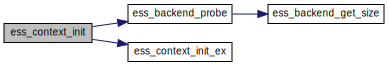
\includegraphics[width=350pt]{d7/d36/ess__context_8h_a40a2211f2793b0346c879b61b35ff63e_cgraph}
\end{center}
\end{figure}
\mbox{\Hypertarget{ess__context_8h_a26ae0093adaa4a6945fed6cfd31d4ae7}\label{ess__context_8h_a26ae0093adaa4a6945fed6cfd31d4ae7}} 
\index{ess\+\_\+context.\+h@{ess\+\_\+context.\+h}!ess\+\_\+context\+\_\+init\+\_\+ex@{ess\+\_\+context\+\_\+init\+\_\+ex}}
\index{ess\+\_\+context\+\_\+init\+\_\+ex@{ess\+\_\+context\+\_\+init\+\_\+ex}!ess\+\_\+context.\+h@{ess\+\_\+context.\+h}}
\subsubsection{\texorpdfstring{ess\+\_\+context\+\_\+init\+\_\+ex()}{ess\_context\_init\_ex()}}
{\footnotesize\ttfamily \hyperlink{ess__context_8h_acc807999e4f53d1867abf8a0ac682f33}{ess\+\_\+context\+\_\+error\+\_\+t} ess\+\_\+context\+\_\+init\+\_\+ex (\begin{DoxyParamCaption}\item[{\hyperlink{ess__context_8h_a8a8fec5766c0b3615f8f12f7948e949b}{ess\+\_\+context\+\_\+t} $\ast$}]{context,  }\item[{\hyperlink{ess__backend_8h_ab1487f8c501b38b66796d0fbecb7ed7b}{ess\+\_\+backend\+\_\+facktory\+\_\+t} $\ast$}]{backend }\end{DoxyParamCaption})}



initialisiert the context with a user backend 


\begin{DoxyCode}
\hyperlink{structess__context}{ess\_context\_t} context;
\hyperlink{structess__backend}{ess\_backend\_facktory\_t}* user\_backend = \{ ,,, \};

\hyperlink{ess__context_8h_ac764fbb6b72712d2b755f54c6b240e33}{ess\_context\_create}(&context, ESS\_FORMAT\_STEREO\_92000\_24);

\hyperlink{ess__context_8h_a26ae0093adaa4a6945fed6cfd31d4ae7}{ess\_context\_init\_ex}(&context, user\_backend);
\end{DoxyCode}
 
\begin{DoxyParams}{Parameters}
{\em context} & the context \\
\hline
\end{DoxyParams}
\begin{DoxyReturn}{Returns}
when ok then E\+S\+S\+\_\+\+C\+O\+N\+T\+E\+X\+T\+\_\+\+E\+R\+R\+O\+R\+\_\+\+OK 
\end{DoxyReturn}


Definition at line 59 of file ess\+\_\+context.\+c.


\begin{DoxyCode}
59                                                                                                  \{
60   \textcolor{keywordflow}{if}(backend == 0 && backend == 0) \{
61     context->\hyperlink{structess__context_a7a8b9bb3789092b56f6a6623888fcc3d}{last\_error} = \hyperlink{ess__context_8h_a4b185bc84680674eb2efc8f720d3362ba29dbe40f674348273f3b23c9c5fcf62d}{ESS\_CONTEXT\_ERRORNOBACKEND};
62     \textcolor{keywordflow}{return} \hyperlink{ess__context_8h_a4b185bc84680674eb2efc8f720d3362ba29dbe40f674348273f3b23c9c5fcf62d}{ESS\_CONTEXT\_ERRORNOBACKEND};
63   \}
64 
65   \textcolor{keywordflow}{if}(backend->\hyperlink{structess__backend_ae6dfe97715fbf9f3fbf7b46a2d311e64}{ess\_backend\_open}(context->\hyperlink{structess__context_abb4395d1c05d3bbc2e1d011507ddd19b}{format}) != 0) \{
66     ESP\_LOGE(\hyperlink{ess__context_8c_a7ce0df38eb467e59f209470c8f5ac4e6}{LOG\_TAG},\textcolor{stringliteral}{"Error to open backend"});
67     \textcolor{keywordflow}{return} -1;
68   \} \textcolor{keywordflow}{else} \{
69 
70     context->\hyperlink{structess__context_a1fdb06c6d95c1f47d692da94aaf8af17}{backend} = backend;
71     context->\hyperlink{structess__context_a6151ccede5aaf683375710d2677c74c7}{status} = \hyperlink{ess__context_8h_a55313861d12b8c596371cace86eacc2eada32323ceb7303d5432781a25cef7f65}{ESS\_CONTEXT\_STATUS\_RUN};
72     
73   \}
74   context->\hyperlink{structess__context_a7a8b9bb3789092b56f6a6623888fcc3d}{last\_error} = \hyperlink{ess__context_8h_a4b185bc84680674eb2efc8f720d3362ba5fbe734224f5adb51e59c6dd88506d60}{ESS\_CONTEXT\_ERROR\_OK};
75   \textcolor{keywordflow}{return} \hyperlink{ess__context_8h_a4b185bc84680674eb2efc8f720d3362ba5fbe734224f5adb51e59c6dd88506d60}{ESS\_CONTEXT\_ERROR\_OK};
76 \}
\end{DoxyCode}
Here is the caller graph for this function\+:
\nopagebreak
\begin{figure}[H]
\begin{center}
\leavevmode
\includegraphics[width=308pt]{d7/d36/ess__context_8h_a26ae0093adaa4a6945fed6cfd31d4ae7_icgraph}
\end{center}
\end{figure}
\mbox{\Hypertarget{ess__context_8h_a6b450cd4cfd4fed931f99b05c38e0172}\label{ess__context_8h_a6b450cd4cfd4fed931f99b05c38e0172}} 
\index{ess\+\_\+context.\+h@{ess\+\_\+context.\+h}!ess\+\_\+context\+\_\+paused@{ess\+\_\+context\+\_\+paused}}
\index{ess\+\_\+context\+\_\+paused@{ess\+\_\+context\+\_\+paused}!ess\+\_\+context.\+h@{ess\+\_\+context.\+h}}
\subsubsection{\texorpdfstring{ess\+\_\+context\+\_\+paused()}{ess\_context\_paused()}}
{\footnotesize\ttfamily \hyperlink{ess__context_8h_acc807999e4f53d1867abf8a0ac682f33}{ess\+\_\+context\+\_\+error\+\_\+t} ess\+\_\+context\+\_\+paused (\begin{DoxyParamCaption}\item[{\hyperlink{ess__context_8h_a8a8fec5766c0b3615f8f12f7948e949b}{ess\+\_\+context\+\_\+t} $\ast$}]{context }\end{DoxyParamCaption})}



set backend to standby 


\begin{DoxyParams}{Parameters}
{\em context} & the context \\
\hline
\end{DoxyParams}
\begin{DoxyReturn}{Returns}
when ok then E\+S\+S\+\_\+\+C\+O\+N\+T\+E\+X\+T\+\_\+\+E\+R\+R\+O\+R\+\_\+\+OK 
\end{DoxyReturn}


Definition at line 99 of file ess\+\_\+context.\+c.


\begin{DoxyCode}
99                                                                \{
100   \textcolor{keywordflow}{if}(context == 0) \textcolor{keywordflow}{return} \hyperlink{ess__context_8h_a4b185bc84680674eb2efc8f720d3362baa6ed95d92bbe32c445b0adce2fc256ce}{ESS\_CONTEXT\_ERROR};
101   \textcolor{keywordflow}{if}(context->\hyperlink{structess__context_a1fdb06c6d95c1f47d692da94aaf8af17}{backend} == 0)  \textcolor{keywordflow}{return} context->\hyperlink{structess__context_a7a8b9bb3789092b56f6a6623888fcc3d}{last\_error} =  
      \hyperlink{ess__context_8h_a4b185bc84680674eb2efc8f720d3362ba29dbe40f674348273f3b23c9c5fcf62d}{ESS\_CONTEXT\_ERRORNOBACKEND};
102 
103   context->\hyperlink{structess__context_a6151ccede5aaf683375710d2677c74c7}{status} = \hyperlink{ess__context_8h_a55313861d12b8c596371cace86eacc2ea6f6315ef32fd6f85789578726d3d06b9}{ESS\_CONTEXT\_STATUS\_PAUSED};
104   context->\hyperlink{structess__context_a1fdb06c6d95c1f47d692da94aaf8af17}{backend}->\hyperlink{structess__backend_ad263ce89d932658c73be2e5863d0afcf}{ess\_backend\_pause}();
105 
106   context->\hyperlink{structess__context_a7a8b9bb3789092b56f6a6623888fcc3d}{last\_error} = \hyperlink{ess__context_8h_a4b185bc84680674eb2efc8f720d3362ba5fbe734224f5adb51e59c6dd88506d60}{ESS\_CONTEXT\_ERROR\_OK};
107   \textcolor{keywordflow}{return} \hyperlink{ess__context_8h_a4b185bc84680674eb2efc8f720d3362ba5fbe734224f5adb51e59c6dd88506d60}{ESS\_CONTEXT\_ERROR\_OK};
108 \}
\end{DoxyCode}
\mbox{\Hypertarget{ess__context_8h_ac6041313862e70f48b8441df8136b0ba}\label{ess__context_8h_ac6041313862e70f48b8441df8136b0ba}} 
\index{ess\+\_\+context.\+h@{ess\+\_\+context.\+h}!ess\+\_\+context\+\_\+resume@{ess\+\_\+context\+\_\+resume}}
\index{ess\+\_\+context\+\_\+resume@{ess\+\_\+context\+\_\+resume}!ess\+\_\+context.\+h@{ess\+\_\+context.\+h}}
\subsubsection{\texorpdfstring{ess\+\_\+context\+\_\+resume()}{ess\_context\_resume()}}
{\footnotesize\ttfamily \hyperlink{ess__context_8h_acc807999e4f53d1867abf8a0ac682f33}{ess\+\_\+context\+\_\+error\+\_\+t} ess\+\_\+context\+\_\+resume (\begin{DoxyParamCaption}\item[{\hyperlink{ess__context_8h_a8a8fec5766c0b3615f8f12f7948e949b}{ess\+\_\+context\+\_\+t} $\ast$}]{context }\end{DoxyParamCaption})}



set backend to run 


\begin{DoxyParams}{Parameters}
{\em context} & the context \\
\hline
\end{DoxyParams}
\begin{DoxyReturn}{Returns}
when ok then E\+S\+S\+\_\+\+C\+O\+N\+T\+E\+X\+T\+\_\+\+E\+R\+R\+O\+R\+\_\+\+OK 
\end{DoxyReturn}


Definition at line 109 of file ess\+\_\+context.\+c.


\begin{DoxyCode}
109                                                                \{
110   \textcolor{keywordflow}{if}(context == 0) \textcolor{keywordflow}{return} \hyperlink{ess__context_8h_a4b185bc84680674eb2efc8f720d3362baa6ed95d92bbe32c445b0adce2fc256ce}{ESS\_CONTEXT\_ERROR};
111   \textcolor{keywordflow}{if}(context->\hyperlink{structess__context_a1fdb06c6d95c1f47d692da94aaf8af17}{backend} == 0)  \textcolor{keywordflow}{return} context->\hyperlink{structess__context_a7a8b9bb3789092b56f6a6623888fcc3d}{last\_error} =  
      \hyperlink{ess__context_8h_a4b185bc84680674eb2efc8f720d3362ba29dbe40f674348273f3b23c9c5fcf62d}{ESS\_CONTEXT\_ERRORNOBACKEND};
112 
113   context->\hyperlink{structess__context_a6151ccede5aaf683375710d2677c74c7}{status} = \hyperlink{ess__context_8h_a55313861d12b8c596371cace86eacc2eada32323ceb7303d5432781a25cef7f65}{ESS\_CONTEXT\_STATUS\_RUN};
114   context->\hyperlink{structess__context_a1fdb06c6d95c1f47d692da94aaf8af17}{backend}->\hyperlink{structess__backend_ab9a30f8d9f4bd941ae74e3ef0c9d7aa3}{ess\_backend\_resum}();
115 
116   context->\hyperlink{structess__context_a7a8b9bb3789092b56f6a6623888fcc3d}{last\_error} = \hyperlink{ess__context_8h_a4b185bc84680674eb2efc8f720d3362ba5fbe734224f5adb51e59c6dd88506d60}{ESS\_CONTEXT\_ERROR\_OK};
117   \textcolor{keywordflow}{return} \hyperlink{ess__context_8h_a4b185bc84680674eb2efc8f720d3362ba5fbe734224f5adb51e59c6dd88506d60}{ESS\_CONTEXT\_ERROR\_OK};
118 \}
\end{DoxyCode}
\mbox{\Hypertarget{ess__context_8h_aebeaf3ec64fe0e348557884dfa601944}\label{ess__context_8h_aebeaf3ec64fe0e348557884dfa601944}} 
\index{ess\+\_\+context.\+h@{ess\+\_\+context.\+h}!ess\+\_\+context\+\_\+set\+\_\+format@{ess\+\_\+context\+\_\+set\+\_\+format}}
\index{ess\+\_\+context\+\_\+set\+\_\+format@{ess\+\_\+context\+\_\+set\+\_\+format}!ess\+\_\+context.\+h@{ess\+\_\+context.\+h}}
\subsubsection{\texorpdfstring{ess\+\_\+context\+\_\+set\+\_\+format()}{ess\_context\_set\_format()}}
{\footnotesize\ttfamily \hyperlink{ess__context_8h_acc807999e4f53d1867abf8a0ac682f33}{ess\+\_\+context\+\_\+error\+\_\+t} ess\+\_\+context\+\_\+set\+\_\+format (\begin{DoxyParamCaption}\item[{\hyperlink{ess__context_8h_a8a8fec5766c0b3615f8f12f7948e949b}{ess\+\_\+context\+\_\+t} $\ast$}]{context,  }\item[{const \hyperlink{ess__format_8h_ab03f24cb5d42f4448f713bf1ec178163}{ess\+\_\+format\+\_\+t}}]{format }\end{DoxyParamCaption})}



set the sample format to backend 


\begin{DoxyParams}{Parameters}
{\em context} & the context 
\begin{DoxyCode}
\hyperlink{structess__context}{ess\_context\_t} context;

\hyperlink{ess__context_8h_ac764fbb6b72712d2b755f54c6b240e33}{ess\_context\_create}(&context, ESS\_FORMAT\_STEREO\_92000\_24); \textcolor{comment}{// Backend Format}
\hyperlink{ess__context_8h_a26ae0093adaa4a6945fed6cfd31d4ae7}{ess\_context\_init\_ex}(&context, \textcolor{stringliteral}{"uart"}); \textcolor{comment}{// open uart backend}

\hyperlink{ess__context_8h_aebeaf3ec64fe0e348557884dfa601944}{ess\_context\_set\_format}(&context, LOADED\_WAV\_FORMAT);
\end{DoxyCode}
 \\
\hline
{\em format} & the new using format \\
\hline
\end{DoxyParams}
\begin{DoxyReturn}{Returns}
when ok then E\+S\+S\+\_\+\+C\+O\+N\+T\+E\+X\+T\+\_\+\+E\+R\+R\+O\+R\+\_\+\+OK 
\end{DoxyReturn}


Definition at line 120 of file ess\+\_\+context.\+c.


\begin{DoxyCode}
120                                                                                               \{
121   \textcolor{keywordflow}{if}(context == 0) \textcolor{keywordflow}{return} \hyperlink{ess__context_8h_a4b185bc84680674eb2efc8f720d3362baa6ed95d92bbe32c445b0adce2fc256ce}{ESS\_CONTEXT\_ERROR};
122   \textcolor{keywordflow}{if}(context->\hyperlink{structess__context_a1fdb06c6d95c1f47d692da94aaf8af17}{backend} == 0)  \textcolor{keywordflow}{return} context->\hyperlink{structess__context_a7a8b9bb3789092b56f6a6623888fcc3d}{last\_error} =  
      \hyperlink{ess__context_8h_a4b185bc84680674eb2efc8f720d3362ba29dbe40f674348273f3b23c9c5fcf62d}{ESS\_CONTEXT\_ERRORNOBACKEND};
123 
124   \textcolor{keywordflow}{return} (\hyperlink{ess__backend_8h_ab9b737a43ebfa9d220c02a32e79346d8}{ess\_backend\_set\_sample\_format}(context->
      \hyperlink{structess__context_a1fdb06c6d95c1f47d692da94aaf8af17}{backend}, format) != 0) ? \hyperlink{ess__context_8h_a4b185bc84680674eb2efc8f720d3362bace646ce156ae1461491206d2bfa7f902}{ESS\_CONTEXT\_WRONGFORMAT} : 
      \hyperlink{ess__context_8h_a4b185bc84680674eb2efc8f720d3362ba5fbe734224f5adb51e59c6dd88506d60}{ESS\_CONTEXT\_ERROR\_OK};
125 \}
\end{DoxyCode}
Here is the call graph for this function\+:
\nopagebreak
\begin{figure}[H]
\begin{center}
\leavevmode
\includegraphics[width=350pt]{d7/d36/ess__context_8h_aebeaf3ec64fe0e348557884dfa601944_cgraph}
\end{center}
\end{figure}
\mbox{\Hypertarget{ess__context_8h_ae2c6a4e2f8a5128fc1bb05afea5f3c8d}\label{ess__context_8h_ae2c6a4e2f8a5128fc1bb05afea5f3c8d}} 
\index{ess\+\_\+context.\+h@{ess\+\_\+context.\+h}!ess\+\_\+context\+\_\+write@{ess\+\_\+context\+\_\+write}}
\index{ess\+\_\+context\+\_\+write@{ess\+\_\+context\+\_\+write}!ess\+\_\+context.\+h@{ess\+\_\+context.\+h}}
\subsubsection{\texorpdfstring{ess\+\_\+context\+\_\+write()}{ess\_context\_write()}}
{\footnotesize\ttfamily unsigned int ess\+\_\+context\+\_\+write (\begin{DoxyParamCaption}\item[{\hyperlink{ess__context_8h_a8a8fec5766c0b3615f8f12f7948e949b}{ess\+\_\+context\+\_\+t} $\ast$}]{context,  }\item[{void $\ast$}]{buffer,  }\item[{unsigned int}]{buf\+\_\+size }\end{DoxyParamCaption})}



write audio data to the backend 


\begin{DoxyParams}{Parameters}
{\em context} & the context \\
\hline
{\em buffer} & the audio pcm data \\
\hline
{\em buf\+\_\+size} & the size of the buffer \\
\hline
\end{DoxyParams}
\begin{DoxyReturn}{Returns}
the written data. 
\end{DoxyReturn}


Definition at line 127 of file ess\+\_\+context.\+c.


\begin{DoxyCode}
127                                                                                             \{
128   \textcolor{keywordtype}{unsigned} \textcolor{keywordtype}{int} wrote;
129   \hyperlink{ess__context_8c_a8077482da675241fd832152974033994}{ess\_context\_write\_ex}(context, buffer, buf\_size, &wrote);
130   \textcolor{keywordflow}{return} wrote;
131 \}
\end{DoxyCode}
Here is the call graph for this function\+:
\nopagebreak
\begin{figure}[H]
\begin{center}
\leavevmode
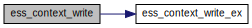
\includegraphics[width=324pt]{d7/d36/ess__context_8h_ae2c6a4e2f8a5128fc1bb05afea5f3c8d_cgraph}
\end{center}
\end{figure}
\mbox{\Hypertarget{ess__context_8h_a8077482da675241fd832152974033994}\label{ess__context_8h_a8077482da675241fd832152974033994}} 
\index{ess\+\_\+context.\+h@{ess\+\_\+context.\+h}!ess\+\_\+context\+\_\+write\+\_\+ex@{ess\+\_\+context\+\_\+write\+\_\+ex}}
\index{ess\+\_\+context\+\_\+write\+\_\+ex@{ess\+\_\+context\+\_\+write\+\_\+ex}!ess\+\_\+context.\+h@{ess\+\_\+context.\+h}}
\subsubsection{\texorpdfstring{ess\+\_\+context\+\_\+write\+\_\+ex()}{ess\_context\_write\_ex()}}
{\footnotesize\ttfamily \hyperlink{ess__context_8h_acc807999e4f53d1867abf8a0ac682f33}{ess\+\_\+context\+\_\+error\+\_\+t} ess\+\_\+context\+\_\+write\+\_\+ex (\begin{DoxyParamCaption}\item[{\hyperlink{ess__context_8h_a8a8fec5766c0b3615f8f12f7948e949b}{ess\+\_\+context\+\_\+t} $\ast$}]{context,  }\item[{void $\ast$}]{buffer,  }\item[{unsigned int}]{buf\+\_\+size,  }\item[{unsigned int $\ast$}]{wrote }\end{DoxyParamCaption})}



write audio data to the backend 


\begin{DoxyParams}{Parameters}
{\em context} & the context \\
\hline
{\em buffer} & the audio pcm data \\
\hline
{\em buf\+\_\+size} & the size of the buffer \\
\hline
{\em wrote} & the written data \\
\hline
\end{DoxyParams}
\begin{DoxyReturn}{Returns}
when ok then E\+S\+S\+\_\+\+C\+O\+N\+T\+E\+X\+T\+\_\+\+E\+R\+R\+O\+R\+\_\+\+OK 
\end{DoxyReturn}


Definition at line 132 of file ess\+\_\+context.\+c.


\begin{DoxyCode}
132                                                                                                            
                       \{
133   \textcolor{keywordflow}{if}(context == 0) \textcolor{keywordflow}{return} \hyperlink{ess__context_8h_a4b185bc84680674eb2efc8f720d3362baa6ed95d92bbe32c445b0adce2fc256ce}{ESS\_CONTEXT\_ERROR};
134   \textcolor{keywordflow}{if}(context->\hyperlink{structess__context_a6151ccede5aaf683375710d2677c74c7}{status} == \hyperlink{ess__context_8h_a55313861d12b8c596371cace86eacc2ea6f6315ef32fd6f85789578726d3d06b9}{ESS\_CONTEXT\_STATUS\_PAUSED}) \textcolor{keywordflow}{return} context->
      \hyperlink{structess__context_a7a8b9bb3789092b56f6a6623888fcc3d}{last\_error} = \hyperlink{ess__context_8h_a4b185bc84680674eb2efc8f720d3362baf33b77dd00f57d9dd7ab4909e3559dae}{ESS\_CONTEX\_ISPAUSED};
135   \textcolor{keywordflow}{if}(context->\hyperlink{structess__context_a1fdb06c6d95c1f47d692da94aaf8af17}{backend} == 0)  \textcolor{keywordflow}{return} context->\hyperlink{structess__context_a7a8b9bb3789092b56f6a6623888fcc3d}{last\_error} =  
      \hyperlink{ess__context_8h_a4b185bc84680674eb2efc8f720d3362ba29dbe40f674348273f3b23c9c5fcf62d}{ESS\_CONTEXT\_ERRORNOBACKEND};
136 
137   context->\hyperlink{structess__context_a1fdb06c6d95c1f47d692da94aaf8af17}{backend}->\hyperlink{structess__backend_a3a1b32830c82ec84aa0e6c02280d7f6c}{ess\_backend\_write}(buffer, buf\_size, wrote);
138 
139   \textcolor{keywordflow}{return}  \hyperlink{ess__context_8h_a4b185bc84680674eb2efc8f720d3362ba5fbe734224f5adb51e59c6dd88506d60}{ESS\_CONTEXT\_ERROR\_OK};
140 \}
\end{DoxyCode}
Here is the caller graph for this function\+:
\nopagebreak
\begin{figure}[H]
\begin{center}
\leavevmode
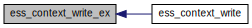
\includegraphics[width=324pt]{d7/d36/ess__context_8h_a8077482da675241fd832152974033994_icgraph}
\end{center}
\end{figure}

\hypertarget{ess__format_8h}{}\section{include/ess\+\_\+format.h File Reference}
\label{ess__format_8h}\index{include/ess\+\_\+format.\+h@{include/ess\+\_\+format.\+h}}
This graph shows which files directly or indirectly include this file\+:
\nopagebreak
\begin{figure}[H]
\begin{center}
\leavevmode
\includegraphics[width=350pt]{d4/d71/ess__format_8h__dep__incl}
\end{center}
\end{figure}
\subsection*{Typedefs}
\begin{DoxyCompactItemize}
\item 
typedef enum \hyperlink{ess__format_8h_aa73ee1bade9564053c023e42c9ea1ec9}{ess\+\_\+format} \hyperlink{ess__format_8h_a9aa23f58a25b9e8360c1400e0cadfd80}{ess\+\_\+format\+\_\+t}
\begin{DoxyCompactList}\small\item\em Audio Format list. \end{DoxyCompactList}\end{DoxyCompactItemize}
\subsection*{Enumerations}
\begin{DoxyCompactItemize}
\item 
enum \hyperlink{ess__format_8h_aa73ee1bade9564053c023e42c9ea1ec9}{ess\+\_\+format} \{ \newline
\hyperlink{ess__format_8h_aa73ee1bade9564053c023e42c9ea1ec9a892a3763a80c8fffbf4a9a9610fca581}{E\+S\+S\+\_\+\+F\+O\+R\+M\+A\+T\+\_\+\+M\+O\+N\+O\+\_\+44100\+\_\+8} = 0, 
\hyperlink{ess__format_8h_aa73ee1bade9564053c023e42c9ea1ec9a99732198d6ef636a40b2566e7d5e3228}{E\+S\+S\+\_\+\+F\+O\+R\+M\+A\+T\+\_\+\+M\+O\+N\+O\+\_\+44100\+\_\+16} = 1, 
\hyperlink{ess__format_8h_aa73ee1bade9564053c023e42c9ea1ec9af986d98b5c2831b1c3cf3eec16869ec1}{E\+S\+S\+\_\+\+F\+O\+R\+M\+A\+T\+\_\+\+M\+O\+N\+O\+\_\+44100\+\_\+24} = 2, 
\hyperlink{ess__format_8h_aa73ee1bade9564053c023e42c9ea1ec9aeb9d0b6147a71b572a0abc1db42a1f00}{E\+S\+S\+\_\+\+F\+O\+R\+M\+A\+T\+\_\+\+M\+O\+N\+O\+\_\+48000\+\_\+8} = 3, 
\newline
\hyperlink{ess__format_8h_aa73ee1bade9564053c023e42c9ea1ec9ab7c50483a73081b56e27690f4e43208d}{E\+S\+S\+\_\+\+F\+O\+R\+M\+A\+T\+\_\+\+M\+O\+N\+O\+\_\+48000\+\_\+16} = 4, 
\hyperlink{ess__format_8h_aa73ee1bade9564053c023e42c9ea1ec9acda2a1f522c223466d6d5302e3ea6a1c}{E\+S\+S\+\_\+\+F\+O\+R\+M\+A\+T\+\_\+\+M\+O\+N\+O\+\_\+48000\+\_\+24} = 5, 
\hyperlink{ess__format_8h_aa73ee1bade9564053c023e42c9ea1ec9a72a28ed1b546e5d793289378a09a4941}{E\+S\+S\+\_\+\+F\+O\+R\+M\+A\+T\+\_\+\+M\+O\+N\+O\+\_\+96000\+\_\+8} = 6, 
\hyperlink{ess__format_8h_aa73ee1bade9564053c023e42c9ea1ec9a2363f289017decd5d0a4296748111389}{E\+S\+S\+\_\+\+F\+O\+R\+M\+A\+T\+\_\+\+M\+O\+N\+O\+\_\+96000\+\_\+16} = 7, 
\newline
\hyperlink{ess__format_8h_aa73ee1bade9564053c023e42c9ea1ec9a9fd9d882c27c0c3751156417c03a0472}{E\+S\+S\+\_\+\+F\+O\+R\+M\+A\+T\+\_\+\+M\+O\+N\+O\+\_\+96000\+\_\+24} = 8, 
\hyperlink{ess__format_8h_aa73ee1bade9564053c023e42c9ea1ec9a2bae9e900e08fc4a602125d80f9d9b45}{E\+S\+S\+\_\+\+F\+O\+R\+M\+A\+T\+\_\+\+S\+T\+E\+R\+E\+O\+\_\+44100\+\_\+8} = 9, 
\hyperlink{ess__format_8h_aa73ee1bade9564053c023e42c9ea1ec9ab4ad20e82e0980a848fb7fe80d0b3377}{E\+S\+S\+\_\+\+F\+O\+R\+M\+A\+T\+\_\+\+S\+T\+E\+R\+E\+O\+\_\+44100\+\_\+16} = 10, 
\hyperlink{ess__format_8h_aa73ee1bade9564053c023e42c9ea1ec9aed7875b085fe5561e16739527ca93b14}{E\+S\+S\+\_\+\+F\+O\+R\+M\+A\+T\+\_\+\+S\+T\+E\+R\+E\+O\+\_\+44100\+\_\+24} = 11, 
\newline
\hyperlink{ess__format_8h_aa73ee1bade9564053c023e42c9ea1ec9af273b9617ff550809968dd34738c67da}{E\+S\+S\+\_\+\+F\+O\+R\+M\+A\+T\+\_\+\+S\+T\+E\+R\+E\+O\+\_\+48000\+\_\+8} = 12, 
\hyperlink{ess__format_8h_aa73ee1bade9564053c023e42c9ea1ec9a1190786d8264fa322c154f531d4bab32}{E\+S\+S\+\_\+\+F\+O\+R\+M\+A\+T\+\_\+\+S\+T\+E\+R\+E\+O\+\_\+48000\+\_\+16} = 13, 
\hyperlink{ess__format_8h_aa73ee1bade9564053c023e42c9ea1ec9a9615ceae2d1180f76e3cffca06625706}{E\+S\+S\+\_\+\+F\+O\+R\+M\+A\+T\+\_\+\+S\+T\+E\+R\+E\+O\+\_\+48000\+\_\+24} = 14, 
\hyperlink{ess__format_8h_aa73ee1bade9564053c023e42c9ea1ec9a52e1c0bb8f510fdaed97ff33220e0783}{E\+S\+S\+\_\+\+F\+O\+R\+M\+A\+T\+\_\+\+S\+T\+E\+R\+E\+O\+\_\+96000\+\_\+8} = 15, 
\newline
\hyperlink{ess__format_8h_aa73ee1bade9564053c023e42c9ea1ec9a95f4383e32c5243da6c704ac89cc6ffe}{E\+S\+S\+\_\+\+F\+O\+R\+M\+A\+T\+\_\+\+S\+T\+E\+R\+E\+O\+\_\+96000\+\_\+16} = 16, 
\hyperlink{ess__format_8h_aa73ee1bade9564053c023e42c9ea1ec9a581a54f1e45f6ab20843028da0b88438}{E\+S\+S\+\_\+\+F\+O\+R\+M\+A\+T\+\_\+\+S\+T\+E\+R\+E\+O\+\_\+96000\+\_\+24} = 17, 
\hyperlink{ess__format_8h_aa73ee1bade9564053c023e42c9ea1ec9af085ca601a7ffc0f56098536616c3a3a}{E\+S\+S\+\_\+\+F\+O\+R\+M\+A\+T\+\_\+\+M\+AX} = 18
 \}\begin{DoxyCompactList}\small\item\em Audio Format list. \end{DoxyCompactList}
\end{DoxyCompactItemize}
\subsection*{Functions}
\begin{DoxyCompactItemize}
\item 
int \hyperlink{ess__format_8h_af1af5721aa4c3a136fef2b5eec4e5a91}{ess\+\_\+format\+\_\+get\+\_\+channels} (const \hyperlink{ess__format_8h_a9aa23f58a25b9e8360c1400e0cadfd80}{ess\+\_\+format\+\_\+t} format)
\begin{DoxyCompactList}\small\item\em Help to get the number of channels of the format. \end{DoxyCompactList}\item 
int \hyperlink{ess__format_8h_a8a38ecc33aa70a8f9497d350706b6463}{ess\+\_\+format\+\_\+get\+\_\+samplerate} (const \hyperlink{ess__format_8h_a9aa23f58a25b9e8360c1400e0cadfd80}{ess\+\_\+format\+\_\+t} format)
\begin{DoxyCompactList}\small\item\em Help to get the samplerate of the format. \end{DoxyCompactList}\item 
int \hyperlink{ess__format_8h_a57f133a9941097d8edc520a1769f0b16}{ess\+\_\+format\+\_\+get\+\_\+bits} (const \hyperlink{ess__format_8h_a9aa23f58a25b9e8360c1400e0cadfd80}{ess\+\_\+format\+\_\+t} format)
\begin{DoxyCompactList}\small\item\em Help to get bits of the format. \end{DoxyCompactList}\item 
const char $\ast$ \hyperlink{ess__format_8h_af281a1ccc7baa8074d7277c065d879e8}{ess\+\_\+format\+\_\+to\+\_\+string} (const \hyperlink{ess__format_8h_a9aa23f58a25b9e8360c1400e0cadfd80}{ess\+\_\+format\+\_\+t} format)
\begin{DoxyCompactList}\small\item\em Help to get the string of the format. \end{DoxyCompactList}\end{DoxyCompactItemize}


\subsection{Typedef Documentation}
\mbox{\Hypertarget{ess__format_8h_a9aa23f58a25b9e8360c1400e0cadfd80}\label{ess__format_8h_a9aa23f58a25b9e8360c1400e0cadfd80}} 
\index{ess\+\_\+format.\+h@{ess\+\_\+format.\+h}!ess\+\_\+format\+\_\+t@{ess\+\_\+format\+\_\+t}}
\index{ess\+\_\+format\+\_\+t@{ess\+\_\+format\+\_\+t}!ess\+\_\+format.\+h@{ess\+\_\+format.\+h}}
\subsubsection{\texorpdfstring{ess\+\_\+format\+\_\+t}{ess\_format\_t}}
{\footnotesize\ttfamily typedef enum \hyperlink{ess__format_8h_aa73ee1bade9564053c023e42c9ea1ec9}{ess\+\_\+format}  \hyperlink{ess__format_8h_a9aa23f58a25b9e8360c1400e0cadfd80}{ess\+\_\+format\+\_\+t}}



Audio Format list. 



\subsection{Enumeration Type Documentation}
\mbox{\Hypertarget{ess__format_8h_aa73ee1bade9564053c023e42c9ea1ec9}\label{ess__format_8h_aa73ee1bade9564053c023e42c9ea1ec9}} 
\index{ess\+\_\+format.\+h@{ess\+\_\+format.\+h}!ess\+\_\+format@{ess\+\_\+format}}
\index{ess\+\_\+format@{ess\+\_\+format}!ess\+\_\+format.\+h@{ess\+\_\+format.\+h}}
\subsubsection{\texorpdfstring{ess\+\_\+format}{ess\_format}}
{\footnotesize\ttfamily enum \hyperlink{ess__format_8h_aa73ee1bade9564053c023e42c9ea1ec9}{ess\+\_\+format}}



Audio Format list. 

\begin{DoxyEnumFields}{Enumerator}
\raisebox{\heightof{T}}[0pt][0pt]{\index{E\+S\+S\+\_\+\+F\+O\+R\+M\+A\+T\+\_\+\+M\+O\+N\+O\+\_\+44100\+\_\+8@{E\+S\+S\+\_\+\+F\+O\+R\+M\+A\+T\+\_\+\+M\+O\+N\+O\+\_\+44100\+\_\+8}!ess\+\_\+format.\+h@{ess\+\_\+format.\+h}}\index{ess\+\_\+format.\+h@{ess\+\_\+format.\+h}!E\+S\+S\+\_\+\+F\+O\+R\+M\+A\+T\+\_\+\+M\+O\+N\+O\+\_\+44100\+\_\+8@{E\+S\+S\+\_\+\+F\+O\+R\+M\+A\+T\+\_\+\+M\+O\+N\+O\+\_\+44100\+\_\+8}}}\mbox{\Hypertarget{ess__format_8h_aa73ee1bade9564053c023e42c9ea1ec9a892a3763a80c8fffbf4a9a9610fca581}\label{ess__format_8h_aa73ee1bade9564053c023e42c9ea1ec9a892a3763a80c8fffbf4a9a9610fca581}} 
E\+S\+S\+\_\+\+F\+O\+R\+M\+A\+T\+\_\+\+M\+O\+N\+O\+\_\+44100\+\_\+8&samplerate 44100 8 Bit Mono \\
\hline

\raisebox{\heightof{T}}[0pt][0pt]{\index{E\+S\+S\+\_\+\+F\+O\+R\+M\+A\+T\+\_\+\+M\+O\+N\+O\+\_\+44100\+\_\+16@{E\+S\+S\+\_\+\+F\+O\+R\+M\+A\+T\+\_\+\+M\+O\+N\+O\+\_\+44100\+\_\+16}!ess\+\_\+format.\+h@{ess\+\_\+format.\+h}}\index{ess\+\_\+format.\+h@{ess\+\_\+format.\+h}!E\+S\+S\+\_\+\+F\+O\+R\+M\+A\+T\+\_\+\+M\+O\+N\+O\+\_\+44100\+\_\+16@{E\+S\+S\+\_\+\+F\+O\+R\+M\+A\+T\+\_\+\+M\+O\+N\+O\+\_\+44100\+\_\+16}}}\mbox{\Hypertarget{ess__format_8h_aa73ee1bade9564053c023e42c9ea1ec9a99732198d6ef636a40b2566e7d5e3228}\label{ess__format_8h_aa73ee1bade9564053c023e42c9ea1ec9a99732198d6ef636a40b2566e7d5e3228}} 
E\+S\+S\+\_\+\+F\+O\+R\+M\+A\+T\+\_\+\+M\+O\+N\+O\+\_\+44100\+\_\+16&samplerate 44100 16 Bit Mono \\
\hline

\raisebox{\heightof{T}}[0pt][0pt]{\index{E\+S\+S\+\_\+\+F\+O\+R\+M\+A\+T\+\_\+\+M\+O\+N\+O\+\_\+44100\+\_\+24@{E\+S\+S\+\_\+\+F\+O\+R\+M\+A\+T\+\_\+\+M\+O\+N\+O\+\_\+44100\+\_\+24}!ess\+\_\+format.\+h@{ess\+\_\+format.\+h}}\index{ess\+\_\+format.\+h@{ess\+\_\+format.\+h}!E\+S\+S\+\_\+\+F\+O\+R\+M\+A\+T\+\_\+\+M\+O\+N\+O\+\_\+44100\+\_\+24@{E\+S\+S\+\_\+\+F\+O\+R\+M\+A\+T\+\_\+\+M\+O\+N\+O\+\_\+44100\+\_\+24}}}\mbox{\Hypertarget{ess__format_8h_aa73ee1bade9564053c023e42c9ea1ec9af986d98b5c2831b1c3cf3eec16869ec1}\label{ess__format_8h_aa73ee1bade9564053c023e42c9ea1ec9af986d98b5c2831b1c3cf3eec16869ec1}} 
E\+S\+S\+\_\+\+F\+O\+R\+M\+A\+T\+\_\+\+M\+O\+N\+O\+\_\+44100\+\_\+24&samplerate 44100 24 Bit Mono \\
\hline

\raisebox{\heightof{T}}[0pt][0pt]{\index{E\+S\+S\+\_\+\+F\+O\+R\+M\+A\+T\+\_\+\+M\+O\+N\+O\+\_\+48000\+\_\+8@{E\+S\+S\+\_\+\+F\+O\+R\+M\+A\+T\+\_\+\+M\+O\+N\+O\+\_\+48000\+\_\+8}!ess\+\_\+format.\+h@{ess\+\_\+format.\+h}}\index{ess\+\_\+format.\+h@{ess\+\_\+format.\+h}!E\+S\+S\+\_\+\+F\+O\+R\+M\+A\+T\+\_\+\+M\+O\+N\+O\+\_\+48000\+\_\+8@{E\+S\+S\+\_\+\+F\+O\+R\+M\+A\+T\+\_\+\+M\+O\+N\+O\+\_\+48000\+\_\+8}}}\mbox{\Hypertarget{ess__format_8h_aa73ee1bade9564053c023e42c9ea1ec9aeb9d0b6147a71b572a0abc1db42a1f00}\label{ess__format_8h_aa73ee1bade9564053c023e42c9ea1ec9aeb9d0b6147a71b572a0abc1db42a1f00}} 
E\+S\+S\+\_\+\+F\+O\+R\+M\+A\+T\+\_\+\+M\+O\+N\+O\+\_\+48000\+\_\+8&samplerate 48000 8 Bit Mono \\
\hline

\raisebox{\heightof{T}}[0pt][0pt]{\index{E\+S\+S\+\_\+\+F\+O\+R\+M\+A\+T\+\_\+\+M\+O\+N\+O\+\_\+48000\+\_\+16@{E\+S\+S\+\_\+\+F\+O\+R\+M\+A\+T\+\_\+\+M\+O\+N\+O\+\_\+48000\+\_\+16}!ess\+\_\+format.\+h@{ess\+\_\+format.\+h}}\index{ess\+\_\+format.\+h@{ess\+\_\+format.\+h}!E\+S\+S\+\_\+\+F\+O\+R\+M\+A\+T\+\_\+\+M\+O\+N\+O\+\_\+48000\+\_\+16@{E\+S\+S\+\_\+\+F\+O\+R\+M\+A\+T\+\_\+\+M\+O\+N\+O\+\_\+48000\+\_\+16}}}\mbox{\Hypertarget{ess__format_8h_aa73ee1bade9564053c023e42c9ea1ec9ab7c50483a73081b56e27690f4e43208d}\label{ess__format_8h_aa73ee1bade9564053c023e42c9ea1ec9ab7c50483a73081b56e27690f4e43208d}} 
E\+S\+S\+\_\+\+F\+O\+R\+M\+A\+T\+\_\+\+M\+O\+N\+O\+\_\+48000\+\_\+16&samplerate 48000 16 Bit Mono \\
\hline

\raisebox{\heightof{T}}[0pt][0pt]{\index{E\+S\+S\+\_\+\+F\+O\+R\+M\+A\+T\+\_\+\+M\+O\+N\+O\+\_\+48000\+\_\+24@{E\+S\+S\+\_\+\+F\+O\+R\+M\+A\+T\+\_\+\+M\+O\+N\+O\+\_\+48000\+\_\+24}!ess\+\_\+format.\+h@{ess\+\_\+format.\+h}}\index{ess\+\_\+format.\+h@{ess\+\_\+format.\+h}!E\+S\+S\+\_\+\+F\+O\+R\+M\+A\+T\+\_\+\+M\+O\+N\+O\+\_\+48000\+\_\+24@{E\+S\+S\+\_\+\+F\+O\+R\+M\+A\+T\+\_\+\+M\+O\+N\+O\+\_\+48000\+\_\+24}}}\mbox{\Hypertarget{ess__format_8h_aa73ee1bade9564053c023e42c9ea1ec9acda2a1f522c223466d6d5302e3ea6a1c}\label{ess__format_8h_aa73ee1bade9564053c023e42c9ea1ec9acda2a1f522c223466d6d5302e3ea6a1c}} 
E\+S\+S\+\_\+\+F\+O\+R\+M\+A\+T\+\_\+\+M\+O\+N\+O\+\_\+48000\+\_\+24&samplerate 48000 24 Bit Mono \\
\hline

\raisebox{\heightof{T}}[0pt][0pt]{\index{E\+S\+S\+\_\+\+F\+O\+R\+M\+A\+T\+\_\+\+M\+O\+N\+O\+\_\+96000\+\_\+8@{E\+S\+S\+\_\+\+F\+O\+R\+M\+A\+T\+\_\+\+M\+O\+N\+O\+\_\+96000\+\_\+8}!ess\+\_\+format.\+h@{ess\+\_\+format.\+h}}\index{ess\+\_\+format.\+h@{ess\+\_\+format.\+h}!E\+S\+S\+\_\+\+F\+O\+R\+M\+A\+T\+\_\+\+M\+O\+N\+O\+\_\+96000\+\_\+8@{E\+S\+S\+\_\+\+F\+O\+R\+M\+A\+T\+\_\+\+M\+O\+N\+O\+\_\+96000\+\_\+8}}}\mbox{\Hypertarget{ess__format_8h_aa73ee1bade9564053c023e42c9ea1ec9a72a28ed1b546e5d793289378a09a4941}\label{ess__format_8h_aa73ee1bade9564053c023e42c9ea1ec9a72a28ed1b546e5d793289378a09a4941}} 
E\+S\+S\+\_\+\+F\+O\+R\+M\+A\+T\+\_\+\+M\+O\+N\+O\+\_\+96000\+\_\+8&samplerate 96000 8 Bit Mono \\
\hline

\raisebox{\heightof{T}}[0pt][0pt]{\index{E\+S\+S\+\_\+\+F\+O\+R\+M\+A\+T\+\_\+\+M\+O\+N\+O\+\_\+96000\+\_\+16@{E\+S\+S\+\_\+\+F\+O\+R\+M\+A\+T\+\_\+\+M\+O\+N\+O\+\_\+96000\+\_\+16}!ess\+\_\+format.\+h@{ess\+\_\+format.\+h}}\index{ess\+\_\+format.\+h@{ess\+\_\+format.\+h}!E\+S\+S\+\_\+\+F\+O\+R\+M\+A\+T\+\_\+\+M\+O\+N\+O\+\_\+96000\+\_\+16@{E\+S\+S\+\_\+\+F\+O\+R\+M\+A\+T\+\_\+\+M\+O\+N\+O\+\_\+96000\+\_\+16}}}\mbox{\Hypertarget{ess__format_8h_aa73ee1bade9564053c023e42c9ea1ec9a2363f289017decd5d0a4296748111389}\label{ess__format_8h_aa73ee1bade9564053c023e42c9ea1ec9a2363f289017decd5d0a4296748111389}} 
E\+S\+S\+\_\+\+F\+O\+R\+M\+A\+T\+\_\+\+M\+O\+N\+O\+\_\+96000\+\_\+16&samplerate 96000 16 Bit Mono \\
\hline

\raisebox{\heightof{T}}[0pt][0pt]{\index{E\+S\+S\+\_\+\+F\+O\+R\+M\+A\+T\+\_\+\+M\+O\+N\+O\+\_\+96000\+\_\+24@{E\+S\+S\+\_\+\+F\+O\+R\+M\+A\+T\+\_\+\+M\+O\+N\+O\+\_\+96000\+\_\+24}!ess\+\_\+format.\+h@{ess\+\_\+format.\+h}}\index{ess\+\_\+format.\+h@{ess\+\_\+format.\+h}!E\+S\+S\+\_\+\+F\+O\+R\+M\+A\+T\+\_\+\+M\+O\+N\+O\+\_\+96000\+\_\+24@{E\+S\+S\+\_\+\+F\+O\+R\+M\+A\+T\+\_\+\+M\+O\+N\+O\+\_\+96000\+\_\+24}}}\mbox{\Hypertarget{ess__format_8h_aa73ee1bade9564053c023e42c9ea1ec9a9fd9d882c27c0c3751156417c03a0472}\label{ess__format_8h_aa73ee1bade9564053c023e42c9ea1ec9a9fd9d882c27c0c3751156417c03a0472}} 
E\+S\+S\+\_\+\+F\+O\+R\+M\+A\+T\+\_\+\+M\+O\+N\+O\+\_\+96000\+\_\+24&samplerate 96000 24 Bit Mono \\
\hline

\raisebox{\heightof{T}}[0pt][0pt]{\index{E\+S\+S\+\_\+\+F\+O\+R\+M\+A\+T\+\_\+\+S\+T\+E\+R\+E\+O\+\_\+44100\+\_\+8@{E\+S\+S\+\_\+\+F\+O\+R\+M\+A\+T\+\_\+\+S\+T\+E\+R\+E\+O\+\_\+44100\+\_\+8}!ess\+\_\+format.\+h@{ess\+\_\+format.\+h}}\index{ess\+\_\+format.\+h@{ess\+\_\+format.\+h}!E\+S\+S\+\_\+\+F\+O\+R\+M\+A\+T\+\_\+\+S\+T\+E\+R\+E\+O\+\_\+44100\+\_\+8@{E\+S\+S\+\_\+\+F\+O\+R\+M\+A\+T\+\_\+\+S\+T\+E\+R\+E\+O\+\_\+44100\+\_\+8}}}\mbox{\Hypertarget{ess__format_8h_aa73ee1bade9564053c023e42c9ea1ec9a2bae9e900e08fc4a602125d80f9d9b45}\label{ess__format_8h_aa73ee1bade9564053c023e42c9ea1ec9a2bae9e900e08fc4a602125d80f9d9b45}} 
E\+S\+S\+\_\+\+F\+O\+R\+M\+A\+T\+\_\+\+S\+T\+E\+R\+E\+O\+\_\+44100\+\_\+8&samplerate 44100 8 Bit Stereo \\
\hline

\raisebox{\heightof{T}}[0pt][0pt]{\index{E\+S\+S\+\_\+\+F\+O\+R\+M\+A\+T\+\_\+\+S\+T\+E\+R\+E\+O\+\_\+44100\+\_\+16@{E\+S\+S\+\_\+\+F\+O\+R\+M\+A\+T\+\_\+\+S\+T\+E\+R\+E\+O\+\_\+44100\+\_\+16}!ess\+\_\+format.\+h@{ess\+\_\+format.\+h}}\index{ess\+\_\+format.\+h@{ess\+\_\+format.\+h}!E\+S\+S\+\_\+\+F\+O\+R\+M\+A\+T\+\_\+\+S\+T\+E\+R\+E\+O\+\_\+44100\+\_\+16@{E\+S\+S\+\_\+\+F\+O\+R\+M\+A\+T\+\_\+\+S\+T\+E\+R\+E\+O\+\_\+44100\+\_\+16}}}\mbox{\Hypertarget{ess__format_8h_aa73ee1bade9564053c023e42c9ea1ec9ab4ad20e82e0980a848fb7fe80d0b3377}\label{ess__format_8h_aa73ee1bade9564053c023e42c9ea1ec9ab4ad20e82e0980a848fb7fe80d0b3377}} 
E\+S\+S\+\_\+\+F\+O\+R\+M\+A\+T\+\_\+\+S\+T\+E\+R\+E\+O\+\_\+44100\+\_\+16&samplerate 44100 16 Bit Stereo \\
\hline

\raisebox{\heightof{T}}[0pt][0pt]{\index{E\+S\+S\+\_\+\+F\+O\+R\+M\+A\+T\+\_\+\+S\+T\+E\+R\+E\+O\+\_\+44100\+\_\+24@{E\+S\+S\+\_\+\+F\+O\+R\+M\+A\+T\+\_\+\+S\+T\+E\+R\+E\+O\+\_\+44100\+\_\+24}!ess\+\_\+format.\+h@{ess\+\_\+format.\+h}}\index{ess\+\_\+format.\+h@{ess\+\_\+format.\+h}!E\+S\+S\+\_\+\+F\+O\+R\+M\+A\+T\+\_\+\+S\+T\+E\+R\+E\+O\+\_\+44100\+\_\+24@{E\+S\+S\+\_\+\+F\+O\+R\+M\+A\+T\+\_\+\+S\+T\+E\+R\+E\+O\+\_\+44100\+\_\+24}}}\mbox{\Hypertarget{ess__format_8h_aa73ee1bade9564053c023e42c9ea1ec9aed7875b085fe5561e16739527ca93b14}\label{ess__format_8h_aa73ee1bade9564053c023e42c9ea1ec9aed7875b085fe5561e16739527ca93b14}} 
E\+S\+S\+\_\+\+F\+O\+R\+M\+A\+T\+\_\+\+S\+T\+E\+R\+E\+O\+\_\+44100\+\_\+24&samplerate 44100 24 Bit Stereo \\
\hline

\raisebox{\heightof{T}}[0pt][0pt]{\index{E\+S\+S\+\_\+\+F\+O\+R\+M\+A\+T\+\_\+\+S\+T\+E\+R\+E\+O\+\_\+48000\+\_\+8@{E\+S\+S\+\_\+\+F\+O\+R\+M\+A\+T\+\_\+\+S\+T\+E\+R\+E\+O\+\_\+48000\+\_\+8}!ess\+\_\+format.\+h@{ess\+\_\+format.\+h}}\index{ess\+\_\+format.\+h@{ess\+\_\+format.\+h}!E\+S\+S\+\_\+\+F\+O\+R\+M\+A\+T\+\_\+\+S\+T\+E\+R\+E\+O\+\_\+48000\+\_\+8@{E\+S\+S\+\_\+\+F\+O\+R\+M\+A\+T\+\_\+\+S\+T\+E\+R\+E\+O\+\_\+48000\+\_\+8}}}\mbox{\Hypertarget{ess__format_8h_aa73ee1bade9564053c023e42c9ea1ec9af273b9617ff550809968dd34738c67da}\label{ess__format_8h_aa73ee1bade9564053c023e42c9ea1ec9af273b9617ff550809968dd34738c67da}} 
E\+S\+S\+\_\+\+F\+O\+R\+M\+A\+T\+\_\+\+S\+T\+E\+R\+E\+O\+\_\+48000\+\_\+8&samplerate 48000 8 Bit Stereo \\
\hline

\raisebox{\heightof{T}}[0pt][0pt]{\index{E\+S\+S\+\_\+\+F\+O\+R\+M\+A\+T\+\_\+\+S\+T\+E\+R\+E\+O\+\_\+48000\+\_\+16@{E\+S\+S\+\_\+\+F\+O\+R\+M\+A\+T\+\_\+\+S\+T\+E\+R\+E\+O\+\_\+48000\+\_\+16}!ess\+\_\+format.\+h@{ess\+\_\+format.\+h}}\index{ess\+\_\+format.\+h@{ess\+\_\+format.\+h}!E\+S\+S\+\_\+\+F\+O\+R\+M\+A\+T\+\_\+\+S\+T\+E\+R\+E\+O\+\_\+48000\+\_\+16@{E\+S\+S\+\_\+\+F\+O\+R\+M\+A\+T\+\_\+\+S\+T\+E\+R\+E\+O\+\_\+48000\+\_\+16}}}\mbox{\Hypertarget{ess__format_8h_aa73ee1bade9564053c023e42c9ea1ec9a1190786d8264fa322c154f531d4bab32}\label{ess__format_8h_aa73ee1bade9564053c023e42c9ea1ec9a1190786d8264fa322c154f531d4bab32}} 
E\+S\+S\+\_\+\+F\+O\+R\+M\+A\+T\+\_\+\+S\+T\+E\+R\+E\+O\+\_\+48000\+\_\+16&samplerate 48000 16 Bit Stereo \\
\hline

\raisebox{\heightof{T}}[0pt][0pt]{\index{E\+S\+S\+\_\+\+F\+O\+R\+M\+A\+T\+\_\+\+S\+T\+E\+R\+E\+O\+\_\+48000\+\_\+24@{E\+S\+S\+\_\+\+F\+O\+R\+M\+A\+T\+\_\+\+S\+T\+E\+R\+E\+O\+\_\+48000\+\_\+24}!ess\+\_\+format.\+h@{ess\+\_\+format.\+h}}\index{ess\+\_\+format.\+h@{ess\+\_\+format.\+h}!E\+S\+S\+\_\+\+F\+O\+R\+M\+A\+T\+\_\+\+S\+T\+E\+R\+E\+O\+\_\+48000\+\_\+24@{E\+S\+S\+\_\+\+F\+O\+R\+M\+A\+T\+\_\+\+S\+T\+E\+R\+E\+O\+\_\+48000\+\_\+24}}}\mbox{\Hypertarget{ess__format_8h_aa73ee1bade9564053c023e42c9ea1ec9a9615ceae2d1180f76e3cffca06625706}\label{ess__format_8h_aa73ee1bade9564053c023e42c9ea1ec9a9615ceae2d1180f76e3cffca06625706}} 
E\+S\+S\+\_\+\+F\+O\+R\+M\+A\+T\+\_\+\+S\+T\+E\+R\+E\+O\+\_\+48000\+\_\+24&samplerate 96000 24 Bit Stereo \\
\hline

\raisebox{\heightof{T}}[0pt][0pt]{\index{E\+S\+S\+\_\+\+F\+O\+R\+M\+A\+T\+\_\+\+S\+T\+E\+R\+E\+O\+\_\+96000\+\_\+8@{E\+S\+S\+\_\+\+F\+O\+R\+M\+A\+T\+\_\+\+S\+T\+E\+R\+E\+O\+\_\+96000\+\_\+8}!ess\+\_\+format.\+h@{ess\+\_\+format.\+h}}\index{ess\+\_\+format.\+h@{ess\+\_\+format.\+h}!E\+S\+S\+\_\+\+F\+O\+R\+M\+A\+T\+\_\+\+S\+T\+E\+R\+E\+O\+\_\+96000\+\_\+8@{E\+S\+S\+\_\+\+F\+O\+R\+M\+A\+T\+\_\+\+S\+T\+E\+R\+E\+O\+\_\+96000\+\_\+8}}}\mbox{\Hypertarget{ess__format_8h_aa73ee1bade9564053c023e42c9ea1ec9a52e1c0bb8f510fdaed97ff33220e0783}\label{ess__format_8h_aa73ee1bade9564053c023e42c9ea1ec9a52e1c0bb8f510fdaed97ff33220e0783}} 
E\+S\+S\+\_\+\+F\+O\+R\+M\+A\+T\+\_\+\+S\+T\+E\+R\+E\+O\+\_\+96000\+\_\+8&samplerate 96000 8 Bit Stereo \\
\hline

\raisebox{\heightof{T}}[0pt][0pt]{\index{E\+S\+S\+\_\+\+F\+O\+R\+M\+A\+T\+\_\+\+S\+T\+E\+R\+E\+O\+\_\+96000\+\_\+16@{E\+S\+S\+\_\+\+F\+O\+R\+M\+A\+T\+\_\+\+S\+T\+E\+R\+E\+O\+\_\+96000\+\_\+16}!ess\+\_\+format.\+h@{ess\+\_\+format.\+h}}\index{ess\+\_\+format.\+h@{ess\+\_\+format.\+h}!E\+S\+S\+\_\+\+F\+O\+R\+M\+A\+T\+\_\+\+S\+T\+E\+R\+E\+O\+\_\+96000\+\_\+16@{E\+S\+S\+\_\+\+F\+O\+R\+M\+A\+T\+\_\+\+S\+T\+E\+R\+E\+O\+\_\+96000\+\_\+16}}}\mbox{\Hypertarget{ess__format_8h_aa73ee1bade9564053c023e42c9ea1ec9a95f4383e32c5243da6c704ac89cc6ffe}\label{ess__format_8h_aa73ee1bade9564053c023e42c9ea1ec9a95f4383e32c5243da6c704ac89cc6ffe}} 
E\+S\+S\+\_\+\+F\+O\+R\+M\+A\+T\+\_\+\+S\+T\+E\+R\+E\+O\+\_\+96000\+\_\+16&samplerate 96000 16 Bit Stereo \\
\hline

\raisebox{\heightof{T}}[0pt][0pt]{\index{E\+S\+S\+\_\+\+F\+O\+R\+M\+A\+T\+\_\+\+S\+T\+E\+R\+E\+O\+\_\+96000\+\_\+24@{E\+S\+S\+\_\+\+F\+O\+R\+M\+A\+T\+\_\+\+S\+T\+E\+R\+E\+O\+\_\+96000\+\_\+24}!ess\+\_\+format.\+h@{ess\+\_\+format.\+h}}\index{ess\+\_\+format.\+h@{ess\+\_\+format.\+h}!E\+S\+S\+\_\+\+F\+O\+R\+M\+A\+T\+\_\+\+S\+T\+E\+R\+E\+O\+\_\+96000\+\_\+24@{E\+S\+S\+\_\+\+F\+O\+R\+M\+A\+T\+\_\+\+S\+T\+E\+R\+E\+O\+\_\+96000\+\_\+24}}}\mbox{\Hypertarget{ess__format_8h_aa73ee1bade9564053c023e42c9ea1ec9a581a54f1e45f6ab20843028da0b88438}\label{ess__format_8h_aa73ee1bade9564053c023e42c9ea1ec9a581a54f1e45f6ab20843028da0b88438}} 
E\+S\+S\+\_\+\+F\+O\+R\+M\+A\+T\+\_\+\+S\+T\+E\+R\+E\+O\+\_\+96000\+\_\+24&samplerate 96000 24 Bit Stereo \\
\hline

\raisebox{\heightof{T}}[0pt][0pt]{\index{E\+S\+S\+\_\+\+F\+O\+R\+M\+A\+T\+\_\+\+M\+AX@{E\+S\+S\+\_\+\+F\+O\+R\+M\+A\+T\+\_\+\+M\+AX}!ess\+\_\+format.\+h@{ess\+\_\+format.\+h}}\index{ess\+\_\+format.\+h@{ess\+\_\+format.\+h}!E\+S\+S\+\_\+\+F\+O\+R\+M\+A\+T\+\_\+\+M\+AX@{E\+S\+S\+\_\+\+F\+O\+R\+M\+A\+T\+\_\+\+M\+AX}}}\mbox{\Hypertarget{ess__format_8h_aa73ee1bade9564053c023e42c9ea1ec9af085ca601a7ffc0f56098536616c3a3a}\label{ess__format_8h_aa73ee1bade9564053c023e42c9ea1ec9af085ca601a7ffc0f56098536616c3a3a}} 
E\+S\+S\+\_\+\+F\+O\+R\+M\+A\+T\+\_\+\+M\+AX&\\
\hline

\end{DoxyEnumFields}


Definition at line 38 of file ess\+\_\+format.\+h.


\begin{DoxyCode}
38                         \{
39    \hyperlink{ess__format_8h_aa73ee1bade9564053c023e42c9ea1ec9a892a3763a80c8fffbf4a9a9610fca581}{ESS\_FORMAT\_MONO\_44100\_8} =                             0 , 
40    \hyperlink{ess__format_8h_aa73ee1bade9564053c023e42c9ea1ec9a99732198d6ef636a40b2566e7d5e3228}{ESS\_FORMAT\_MONO\_44100\_16} =                            1 , 
41    \hyperlink{ess__format_8h_aa73ee1bade9564053c023e42c9ea1ec9af986d98b5c2831b1c3cf3eec16869ec1}{ESS\_FORMAT\_MONO\_44100\_24} =                          2 , 
42    \hyperlink{ess__format_8h_aa73ee1bade9564053c023e42c9ea1ec9aeb9d0b6147a71b572a0abc1db42a1f00}{ESS\_FORMAT\_MONO\_48000\_8}   =                          3 , 
43    \hyperlink{ess__format_8h_aa73ee1bade9564053c023e42c9ea1ec9ab7c50483a73081b56e27690f4e43208d}{ESS\_FORMAT\_MONO\_48000\_16} =                          4 , 
44    \hyperlink{ess__format_8h_aa73ee1bade9564053c023e42c9ea1ec9acda2a1f522c223466d6d5302e3ea6a1c}{ESS\_FORMAT\_MONO\_48000\_24} =                          5 , 
45    \hyperlink{ess__format_8h_aa73ee1bade9564053c023e42c9ea1ec9a72a28ed1b546e5d793289378a09a4941}{ESS\_FORMAT\_MONO\_96000\_8}  =                           6 , 
46    \hyperlink{ess__format_8h_aa73ee1bade9564053c023e42c9ea1ec9a2363f289017decd5d0a4296748111389}{ESS\_FORMAT\_MONO\_96000\_16} =                          7, 
47    \hyperlink{ess__format_8h_aa73ee1bade9564053c023e42c9ea1ec9a9fd9d882c27c0c3751156417c03a0472}{ESS\_FORMAT\_MONO\_96000\_24} =                          8, 
48    \hyperlink{ess__format_8h_aa73ee1bade9564053c023e42c9ea1ec9a2bae9e900e08fc4a602125d80f9d9b45}{ESS\_FORMAT\_STEREO\_44100\_8} =                          9 , 
49    \hyperlink{ess__format_8h_aa73ee1bade9564053c023e42c9ea1ec9ab4ad20e82e0980a848fb7fe80d0b3377}{ESS\_FORMAT\_STEREO\_44100\_16} =                      10 , 
50    \hyperlink{ess__format_8h_aa73ee1bade9564053c023e42c9ea1ec9aed7875b085fe5561e16739527ca93b14}{ESS\_FORMAT\_STEREO\_44100\_24} =                      11 , 
51    \hyperlink{ess__format_8h_aa73ee1bade9564053c023e42c9ea1ec9af273b9617ff550809968dd34738c67da}{ESS\_FORMAT\_STEREO\_48000\_8} =                        12 , 
52    \hyperlink{ess__format_8h_aa73ee1bade9564053c023e42c9ea1ec9a1190786d8264fa322c154f531d4bab32}{ESS\_FORMAT\_STEREO\_48000\_16} =                      13 , 
53    \hyperlink{ess__format_8h_aa73ee1bade9564053c023e42c9ea1ec9a9615ceae2d1180f76e3cffca06625706}{ESS\_FORMAT\_STEREO\_48000\_24} =              14, 
54    \hyperlink{ess__format_8h_aa73ee1bade9564053c023e42c9ea1ec9a52e1c0bb8f510fdaed97ff33220e0783}{ESS\_FORMAT\_STEREO\_96000\_8}  =               15, 
55    \hyperlink{ess__format_8h_aa73ee1bade9564053c023e42c9ea1ec9a95f4383e32c5243da6c704ac89cc6ffe}{ESS\_FORMAT\_STEREO\_96000\_16} =              16, 
56    \hyperlink{ess__format_8h_aa73ee1bade9564053c023e42c9ea1ec9a581a54f1e45f6ab20843028da0b88438}{ESS\_FORMAT\_STEREO\_96000\_24} =              17, 
58    \hyperlink{ess__format_8h_aa73ee1bade9564053c023e42c9ea1ec9af085ca601a7ffc0f56098536616c3a3a}{ESS\_FORMAT\_MAX}  = 18,
59 \} \hyperlink{ess__format_8h_a9aa23f58a25b9e8360c1400e0cadfd80}{ess\_format\_t};
\end{DoxyCode}


\subsection{Function Documentation}
\mbox{\Hypertarget{ess__format_8h_a57f133a9941097d8edc520a1769f0b16}\label{ess__format_8h_a57f133a9941097d8edc520a1769f0b16}} 
\index{ess\+\_\+format.\+h@{ess\+\_\+format.\+h}!ess\+\_\+format\+\_\+get\+\_\+bits@{ess\+\_\+format\+\_\+get\+\_\+bits}}
\index{ess\+\_\+format\+\_\+get\+\_\+bits@{ess\+\_\+format\+\_\+get\+\_\+bits}!ess\+\_\+format.\+h@{ess\+\_\+format.\+h}}
\subsubsection{\texorpdfstring{ess\+\_\+format\+\_\+get\+\_\+bits()}{ess\_format\_get\_bits()}}
{\footnotesize\ttfamily int ess\+\_\+format\+\_\+get\+\_\+bits (\begin{DoxyParamCaption}\item[{const \hyperlink{ess__format_8h_a9aa23f58a25b9e8360c1400e0cadfd80}{ess\+\_\+format\+\_\+t}}]{format }\end{DoxyParamCaption})}



Help to get bits of the format. 


\begin{DoxyParams}{Parameters}
{\em format} & The format to parse \\
\hline
\end{DoxyParams}


Definition at line 68 of file ess\+\_\+format.\+c.


\begin{DoxyCode}
68                                                    \{
69   \textcolor{keywordflow}{if}(format >= \hyperlink{ess__format_8h_aa73ee1bade9564053c023e42c9ea1ec9af085ca601a7ffc0f56098536616c3a3a}{ESS\_FORMAT\_MAX}) \textcolor{keywordflow}{return} -1;
70   \textcolor{keywordflow}{return} \hyperlink{ess__format_8c_afe86278e648eeb366ddc31cb864ec547}{format\_parse}[format].\hyperlink{struct__format2human_ad1e28a1a66a25529b0b61b9ca4e66d44}{bits};
71 \}
\end{DoxyCode}
\mbox{\Hypertarget{ess__format_8h_af1af5721aa4c3a136fef2b5eec4e5a91}\label{ess__format_8h_af1af5721aa4c3a136fef2b5eec4e5a91}} 
\index{ess\+\_\+format.\+h@{ess\+\_\+format.\+h}!ess\+\_\+format\+\_\+get\+\_\+channels@{ess\+\_\+format\+\_\+get\+\_\+channels}}
\index{ess\+\_\+format\+\_\+get\+\_\+channels@{ess\+\_\+format\+\_\+get\+\_\+channels}!ess\+\_\+format.\+h@{ess\+\_\+format.\+h}}
\subsubsection{\texorpdfstring{ess\+\_\+format\+\_\+get\+\_\+channels()}{ess\_format\_get\_channels()}}
{\footnotesize\ttfamily int ess\+\_\+format\+\_\+get\+\_\+channels (\begin{DoxyParamCaption}\item[{const \hyperlink{ess__format_8h_a9aa23f58a25b9e8360c1400e0cadfd80}{ess\+\_\+format\+\_\+t}}]{format }\end{DoxyParamCaption})}



Help to get the number of channels of the format. 


\begin{DoxyParams}{Parameters}
{\em format} & The format to parse \\
\hline
\end{DoxyParams}


Definition at line 59 of file ess\+\_\+format.\+c.


\begin{DoxyCode}
59                                                        \{
60   \textcolor{keywordflow}{if}(format >= \hyperlink{ess__format_8h_aa73ee1bade9564053c023e42c9ea1ec9af085ca601a7ffc0f56098536616c3a3a}{ESS\_FORMAT\_MAX}) \textcolor{keywordflow}{return} -1;
61     \textcolor{keywordflow}{return} \hyperlink{ess__format_8c_afe86278e648eeb366ddc31cb864ec547}{format\_parse}[format].\hyperlink{struct__format2human_a178795099d0608972755dfef8d8367e3}{channels};
62 \}
\end{DoxyCode}
\mbox{\Hypertarget{ess__format_8h_a8a38ecc33aa70a8f9497d350706b6463}\label{ess__format_8h_a8a38ecc33aa70a8f9497d350706b6463}} 
\index{ess\+\_\+format.\+h@{ess\+\_\+format.\+h}!ess\+\_\+format\+\_\+get\+\_\+samplerate@{ess\+\_\+format\+\_\+get\+\_\+samplerate}}
\index{ess\+\_\+format\+\_\+get\+\_\+samplerate@{ess\+\_\+format\+\_\+get\+\_\+samplerate}!ess\+\_\+format.\+h@{ess\+\_\+format.\+h}}
\subsubsection{\texorpdfstring{ess\+\_\+format\+\_\+get\+\_\+samplerate()}{ess\_format\_get\_samplerate()}}
{\footnotesize\ttfamily int ess\+\_\+format\+\_\+get\+\_\+samplerate (\begin{DoxyParamCaption}\item[{const \hyperlink{ess__format_8h_a9aa23f58a25b9e8360c1400e0cadfd80}{ess\+\_\+format\+\_\+t}}]{format }\end{DoxyParamCaption})}



Help to get the samplerate of the format. 


\begin{DoxyParams}{Parameters}
{\em format} & The format to parse \\
\hline
\end{DoxyParams}


Definition at line 63 of file ess\+\_\+format.\+c.


\begin{DoxyCode}
63                                                          \{
64   \textcolor{keywordflow}{if}(format >= \hyperlink{ess__format_8h_aa73ee1bade9564053c023e42c9ea1ec9af085ca601a7ffc0f56098536616c3a3a}{ESS\_FORMAT\_MAX}) \textcolor{keywordflow}{return} -1;
65   \textcolor{keywordflow}{return} \hyperlink{ess__format_8c_afe86278e648eeb366ddc31cb864ec547}{format\_parse}[format].\hyperlink{struct__format2human_ac38751c7169cfeb9325a947cc0484286}{samplerate};
66 \}
\end{DoxyCode}
\mbox{\Hypertarget{ess__format_8h_af281a1ccc7baa8074d7277c065d879e8}\label{ess__format_8h_af281a1ccc7baa8074d7277c065d879e8}} 
\index{ess\+\_\+format.\+h@{ess\+\_\+format.\+h}!ess\+\_\+format\+\_\+to\+\_\+string@{ess\+\_\+format\+\_\+to\+\_\+string}}
\index{ess\+\_\+format\+\_\+to\+\_\+string@{ess\+\_\+format\+\_\+to\+\_\+string}!ess\+\_\+format.\+h@{ess\+\_\+format.\+h}}
\subsubsection{\texorpdfstring{ess\+\_\+format\+\_\+to\+\_\+string()}{ess\_format\_to\_string()}}
{\footnotesize\ttfamily const char$\ast$ ess\+\_\+format\+\_\+to\+\_\+string (\begin{DoxyParamCaption}\item[{const \hyperlink{ess__format_8h_a9aa23f58a25b9e8360c1400e0cadfd80}{ess\+\_\+format\+\_\+t}}]{format }\end{DoxyParamCaption})}



Help to get the string of the format. 


\begin{DoxyParams}{Parameters}
{\em format} & The format to parse \\
\hline
\end{DoxyParams}


Definition at line 76 of file ess\+\_\+format.\+c.


\begin{DoxyCode}
76                                                       \{
77   \textcolor{keywordflow}{if}(format >= \hyperlink{ess__format_8h_aa73ee1bade9564053c023e42c9ea1ec9af085ca601a7ffc0f56098536616c3a3a}{ESS\_FORMAT\_MAX}) \textcolor{keywordflow}{return} \textcolor{stringliteral}{"NO\_FORMAT"};
78   \textcolor{keywordflow}{return} \hyperlink{ess__format_8c_afe86278e648eeb366ddc31cb864ec547}{format\_parse}[format].\hyperlink{struct__format2human_a14f2551e7b5032527b89aa2d4025523a}{string};
79 \}
\end{DoxyCode}
Here is the caller graph for this function\+:
\nopagebreak
\begin{figure}[H]
\begin{center}
\leavevmode
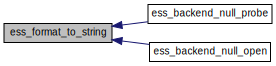
\includegraphics[width=350pt]{d7/d35/ess__format_8h_af281a1ccc7baa8074d7277c065d879e8_icgraph}
\end{center}
\end{figure}

\hypertarget{ess__platform_8h}{}\section{include/ess\+\_\+platform.h File Reference}
\label{ess__platform_8h}\index{include/ess\+\_\+platform.\+h@{include/ess\+\_\+platform.\+h}}


all platform specific functions  


This graph shows which files directly or indirectly include this file\+:\nopagebreak
\begin{figure}[H]
\begin{center}
\leavevmode
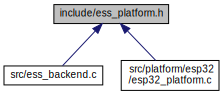
\includegraphics[width=195pt]{dd/da0/ess__platform_8h__dep__incl}
\end{center}
\end{figure}
\subsection*{Data Structures}
\begin{DoxyCompactItemize}
\item 
struct \hyperlink{structess__platform__task}{ess\+\_\+platform\+\_\+task}
\item 
struct \hyperlink{structess__platform__semaphore}{ess\+\_\+platform\+\_\+semaphore}
\item 
struct \hyperlink{structess__platform__ringbuffer}{ess\+\_\+platform\+\_\+ringbuffer}
\end{DoxyCompactItemize}
\subsection*{Typedefs}
\begin{DoxyCompactItemize}
\item 
typedef enum \hyperlink{ess__platform_8h_acf304dba65a175a7844962b5b860c84f}{ess\+\_\+platform\+\_\+error} \hyperlink{ess__platform_8h_a0dea8f0bbcf8468d31552caf9b0cd1b8}{ess\+\_\+platform\+\_\+error\+\_\+t}
\item 
typedef enum \hyperlink{ess__platform_8h_aadec572693e8bd97eefafaacb7049651}{ess\+\_\+platform\+\_\+ringbuffer\+\_\+mode} \hyperlink{ess__platform_8h_a80a1652a42f77e9a51f3e45c7da84396}{ess\+\_\+platform\+\_\+ringbuffer\+\_\+mode\+\_\+t}
\item 
typedef struct \hyperlink{structess__platform__task}{ess\+\_\+platform\+\_\+task} \hyperlink{ess__platform_8h_ae70a08fbb1b43d09d8f0e51c049d1570}{ess\+\_\+platform\+\_\+task\+\_\+t}
\item 
typedef struct \hyperlink{structess__platform__semaphore}{ess\+\_\+platform\+\_\+semaphore} \hyperlink{ess__platform_8h_aeec51ce8d31b1560633f2a57b11c8b12}{ess\+\_\+platform\+\_\+semaphore\+\_\+t}
\item 
typedef struct \hyperlink{structess__platform__ringbuffer}{ess\+\_\+platform\+\_\+ringbuffer} \hyperlink{ess__platform_8h_a9d764d1cfe4ef17268936028a683b7a3}{ess\+\_\+platform\+\_\+ringbuffer\+\_\+t}
\end{DoxyCompactItemize}
\subsection*{Enumerations}
\begin{DoxyCompactItemize}
\item 
enum \hyperlink{ess__platform_8h_acf304dba65a175a7844962b5b860c84f}{ess\+\_\+platform\+\_\+error} \{ \newline
\hyperlink{ess__platform_8h_acf304dba65a175a7844962b5b860c84fa1d99f71b1dc776843a2b54b09a5bc605}{E\+S\+S\+\_\+\+P\+L\+A\+T\+F\+O\+R\+M\+\_\+\+E\+R\+R\+O\+R\+\_\+\+OK} = 0, 
\hyperlink{ess__platform_8h_acf304dba65a175a7844962b5b860c84fa7c577028be43a6226f39286651b542dc}{E\+S\+S\+\_\+\+P\+L\+A\+T\+F\+O\+R\+M\+\_\+\+N\+O\+T\+\_\+\+I\+MP} = -\/1, 
\hyperlink{ess__platform_8h_acf304dba65a175a7844962b5b860c84faefeea534f4705b242dd8eee1de7722d0}{E\+S\+S\+\_\+\+P\+L\+A\+T\+F\+O\+R\+M\+\_\+\+E\+R\+R\+OR}, 
\hyperlink{ess__platform_8h_acf304dba65a175a7844962b5b860c84fa09e852cc66c78c515db90b9365613601}{E\+S\+S\+\_\+\+P\+L\+A\+T\+F\+O\+R\+M\+\_\+\+E\+R\+R\+O\+R\+\_\+\+N\+U\+LL}, 
\newline
\hyperlink{ess__platform_8h_acf304dba65a175a7844962b5b860c84fafdcd168f2a74bb3c5dabfbc3ed613c7b}{E\+S\+S\+\_\+\+P\+L\+A\+T\+F\+O\+R\+M\+\_\+\+N\+O\+T\+\_\+\+C\+R\+E\+A\+T\+ED}
 \}
\item 
enum \hyperlink{ess__platform_8h_aadec572693e8bd97eefafaacb7049651}{ess\+\_\+platform\+\_\+ringbuffer\+\_\+mode} \{ \hyperlink{ess__platform_8h_aadec572693e8bd97eefafaacb7049651aade74af3c687f765e6ed7ae0eaa5d823}{E\+S\+S\+\_\+\+P\+L\+A\+T\+F\+O\+R\+M\+\_\+\+R\+I\+N\+G\+B\+U\+F\+F\+E\+R\+\_\+\+M\+O\+D\+E\+\_\+\+N\+O\+S\+P\+L\+IT}, 
\hyperlink{ess__platform_8h_aadec572693e8bd97eefafaacb7049651a5f516be84e00a92f549871ac6cca35e4}{E\+S\+S\+\_\+\+P\+L\+A\+T\+F\+O\+R\+M\+\_\+\+R\+I\+N\+G\+B\+U\+F\+F\+E\+R\+\_\+\+M\+O\+D\+E\+\_\+\+A\+L\+L\+O\+W\+S\+P\+L\+IT}, 
\hyperlink{ess__platform_8h_aadec572693e8bd97eefafaacb7049651acaa808912c42432dc4cfad09ff10a73f}{E\+S\+S\+\_\+\+P\+L\+A\+T\+F\+O\+R\+M\+\_\+\+R\+I\+N\+G\+B\+U\+F\+F\+E\+R\+\_\+\+M\+O\+D\+E\+\_\+\+B\+Y\+T\+E\+B\+UF}
 \}
\end{DoxyCompactItemize}
\subsection*{Functions}
\begin{DoxyCompactItemize}
\item 
\hyperlink{ess__backend_8h_ab1487f8c501b38b66796d0fbecb7ed7b}{ess\+\_\+backend\+\_\+facktory\+\_\+t} $\ast$ \hyperlink{ess__platform_8h_a76cca5b79ff4c68316ec3284b78d6436}{ess\+\_\+backend\+\_\+null\+\_\+get\+Factory} ()
\item 
unsigned int \hyperlink{ess__platform_8h_a94c4057bf1b7c58588e80bce004f76d3}{ess\+\_\+platform\+\_\+get\+\_\+tick\+\_\+count} ()
\begin{DoxyCompactList}\small\item\em get the time in milliseconds since the Free\+R\+T\+OS scheduler started. \end{DoxyCompactList}\item 
\hyperlink{ess__platform_8h_a0dea8f0bbcf8468d31552caf9b0cd1b8}{ess\+\_\+platform\+\_\+error\+\_\+t} \hyperlink{ess__platform_8h_a5e996530ea97d5c9e6fe1e23fcfc3305}{ess\+\_\+platform\+\_\+sleep} (unsigned int ms)
\begin{DoxyCompactList}\small\item\em Sleep for the specified number of milliseconds. \end{DoxyCompactList}\item 
\hyperlink{ess__platform_8h_a0dea8f0bbcf8468d31552caf9b0cd1b8}{ess\+\_\+platform\+\_\+error\+\_\+t} \hyperlink{ess__platform_8h_a8278147de6a2fd0aff2284865b888600}{ess\+\_\+platform\+\_\+task\+\_\+create} (\hyperlink{ess__platform_8h_ae70a08fbb1b43d09d8f0e51c049d1570}{ess\+\_\+platform\+\_\+task\+\_\+t} $\ast$task, void task\+\_\+func(void $\ast$), const char $\ast$task\+Name, void $\ast$param, unsigned int stack\+Size)
\begin{DoxyCompactList}\small\item\em fill the \textquotesingle{}esp\+\_\+platform\+\_\+task\+\_\+t\textquotesingle{} struct \end{DoxyCompactList}\item 
\hyperlink{ess__platform_8h_a0dea8f0bbcf8468d31552caf9b0cd1b8}{ess\+\_\+platform\+\_\+error\+\_\+t} \hyperlink{ess__platform_8h_ab0829781a10b11e0fdff3736e6e3d33f}{ess\+\_\+platform\+\_\+task\+\_\+start} (\hyperlink{ess__platform_8h_ae70a08fbb1b43d09d8f0e51c049d1570}{ess\+\_\+platform\+\_\+task\+\_\+t} $\ast$task)
\begin{DoxyCompactList}\small\item\em start the task \end{DoxyCompactList}\item 
\hyperlink{ess__platform_8h_a0dea8f0bbcf8468d31552caf9b0cd1b8}{ess\+\_\+platform\+\_\+error\+\_\+t} \hyperlink{ess__platform_8h_a2759a9e11e691d9b66fe2183a00052ce}{ess\+\_\+platform\+\_\+task\+\_\+delete} (\hyperlink{ess__platform_8h_ae70a08fbb1b43d09d8f0e51c049d1570}{ess\+\_\+platform\+\_\+task\+\_\+t} $\ast$task)
\begin{DoxyCompactList}\small\item\em delete the task \end{DoxyCompactList}\item 
\hyperlink{ess__platform_8h_a0dea8f0bbcf8468d31552caf9b0cd1b8}{ess\+\_\+platform\+\_\+error\+\_\+t} \hyperlink{ess__platform_8h_a8fcaa7847cb75e65b97bdbe6e44599ce}{ess\+\_\+platform\+\_\+semaphore\+\_\+create} (\hyperlink{ess__platform_8h_aeec51ce8d31b1560633f2a57b11c8b12}{ess\+\_\+platform\+\_\+semaphore\+\_\+t} $\ast$semp, const char $\ast$name)
\begin{DoxyCompactList}\small\item\em create the semaphore \end{DoxyCompactList}\item 
\hyperlink{ess__platform_8h_a0dea8f0bbcf8468d31552caf9b0cd1b8}{ess\+\_\+platform\+\_\+error\+\_\+t} \hyperlink{ess__platform_8h_aafe4c188af2850b91774a551308bb79c}{ess\+\_\+platform\+\_\+semaphore\+\_\+destroy} (\hyperlink{ess__platform_8h_aeec51ce8d31b1560633f2a57b11c8b12}{ess\+\_\+platform\+\_\+semaphore\+\_\+t} $\ast$semp)
\begin{DoxyCompactList}\small\item\em destroy the semaphore \end{DoxyCompactList}\item 
\hyperlink{ess__platform_8h_a0dea8f0bbcf8468d31552caf9b0cd1b8}{ess\+\_\+platform\+\_\+error\+\_\+t} \hyperlink{ess__platform_8h_a83cec747790472fe5d6225b23b4feabb}{ess\+\_\+platform\+\_\+semaphore\+\_\+take\+\_\+ex} (\hyperlink{ess__platform_8h_aeec51ce8d31b1560633f2a57b11c8b12}{ess\+\_\+platform\+\_\+semaphore\+\_\+t} $\ast$semp, unsigned int timeout\+\_\+ms)
\begin{DoxyCompactList}\small\item\em take a semaphore \end{DoxyCompactList}\item 
\hyperlink{ess__platform_8h_a0dea8f0bbcf8468d31552caf9b0cd1b8}{ess\+\_\+platform\+\_\+error\+\_\+t} \hyperlink{ess__platform_8h_a72920aa7d9fd73a1a2fd3b1658695cdf}{ess\+\_\+platform\+\_\+semaphore\+\_\+take} (\hyperlink{ess__platform_8h_aeec51ce8d31b1560633f2a57b11c8b12}{ess\+\_\+platform\+\_\+semaphore\+\_\+t} $\ast$semp)
\begin{DoxyCompactList}\small\item\em take a semaphore \end{DoxyCompactList}\item 
\hyperlink{ess__platform_8h_a0dea8f0bbcf8468d31552caf9b0cd1b8}{ess\+\_\+platform\+\_\+error\+\_\+t} \hyperlink{ess__platform_8h_a11d1259212ed56ea3aa5333a50279596}{ess\+\_\+platform\+\_\+semaphore\+\_\+give} (\hyperlink{ess__platform_8h_aeec51ce8d31b1560633f2a57b11c8b12}{ess\+\_\+platform\+\_\+semaphore\+\_\+t} $\ast$semp)
\begin{DoxyCompactList}\small\item\em take a semaphore \end{DoxyCompactList}\item 
\hyperlink{ess__platform_8h_a0dea8f0bbcf8468d31552caf9b0cd1b8}{ess\+\_\+platform\+\_\+error\+\_\+t} \hyperlink{ess__platform_8h_a333b338c83550706250a18d8d9b00239}{ess\+\_\+platform\+\_\+semaphore\+\_\+give\+\_\+ex} (\hyperlink{ess__platform_8h_aeec51ce8d31b1560633f2a57b11c8b12}{ess\+\_\+platform\+\_\+semaphore\+\_\+t} $\ast$semp, int value)
\begin{DoxyCompactList}\small\item\em give a semaphore \end{DoxyCompactList}\item 
\hyperlink{ess__platform_8h_a0dea8f0bbcf8468d31552caf9b0cd1b8}{ess\+\_\+platform\+\_\+error\+\_\+t} \hyperlink{ess__platform_8h_ae67ecf51ca686384ec71f63fe763a7a5}{ess\+\_\+platform\+\_\+semaphore\+\_\+give\+\_\+isr} (\hyperlink{ess__platform_8h_aeec51ce8d31b1560633f2a57b11c8b12}{ess\+\_\+platform\+\_\+semaphore\+\_\+t} $\ast$semp)
\begin{DoxyCompactList}\small\item\em give a semaphore from I\+SR \end{DoxyCompactList}\item 
\hyperlink{ess__platform_8h_a0dea8f0bbcf8468d31552caf9b0cd1b8}{ess\+\_\+platform\+\_\+error\+\_\+t} \hyperlink{ess__platform_8h_a8267e0d5bc2ed806dc397cb805dec347}{ess\+\_\+platform\+\_\+semaphore\+\_\+wait} (\hyperlink{ess__platform_8h_aeec51ce8d31b1560633f2a57b11c8b12}{ess\+\_\+platform\+\_\+semaphore\+\_\+t} $\ast$semp, int $\ast$value)
\begin{DoxyCompactList}\small\item\em wait for a semaphore to be released by trying to take it and then releasing it again. \end{DoxyCompactList}\item 
\hyperlink{ess__platform_8h_a0dea8f0bbcf8468d31552caf9b0cd1b8}{ess\+\_\+platform\+\_\+error\+\_\+t} \hyperlink{ess__platform_8h_af13605b4ec395981d2c655df4a0389bd}{ess\+\_\+platform\+\_\+ringbuffer\+\_\+create} (\hyperlink{ess__platform_8h_a9d764d1cfe4ef17268936028a683b7a3}{ess\+\_\+platform\+\_\+ringbuffer\+\_\+t} $\ast$rng, unsigned int length, \hyperlink{ess__platform_8h_a80a1652a42f77e9a51f3e45c7da84396}{ess\+\_\+platform\+\_\+ringbuffer\+\_\+mode\+\_\+t} type, const char $\ast$name)
\begin{DoxyCompactList}\small\item\em Create a ring buffer. \end{DoxyCompactList}\item 
\hyperlink{ess__platform_8h_a0dea8f0bbcf8468d31552caf9b0cd1b8}{ess\+\_\+platform\+\_\+error\+\_\+t} \hyperlink{ess__platform_8h_a3f92242e224b54445ea7d3cd06536276}{ess\+\_\+platform\+\_\+ringbuffer\+\_\+destroy} (\hyperlink{ess__platform_8h_a9d764d1cfe4ef17268936028a683b7a3}{ess\+\_\+platform\+\_\+ringbuffer\+\_\+t} $\ast$rng)
\begin{DoxyCompactList}\small\item\em destroy the ring buffer. \end{DoxyCompactList}\item 
\hyperlink{ess__platform_8h_a0dea8f0bbcf8468d31552caf9b0cd1b8}{ess\+\_\+platform\+\_\+error\+\_\+t} \hyperlink{ess__platform_8h_ad83715b593c0d904151eed8828791c09}{ess\+\_\+platform\+\_\+ringbuffer\+\_\+write} (\hyperlink{ess__platform_8h_a9d764d1cfe4ef17268936028a683b7a3}{ess\+\_\+platform\+\_\+ringbuffer\+\_\+t} $\ast$rng, void $\ast$data, unsigned int length, unsigned int ms)
\begin{DoxyCompactList}\small\item\em write data to the ring buffer. \end{DoxyCompactList}\item 
\hyperlink{ess__platform_8h_a0dea8f0bbcf8468d31552caf9b0cd1b8}{ess\+\_\+platform\+\_\+error\+\_\+t} \hyperlink{ess__platform_8h_a7f35e063b9e8c683e2eec421661cda34}{ess\+\_\+platform\+\_\+ringbuffer\+\_\+can\+\_\+read} (\hyperlink{ess__platform_8h_a9d764d1cfe4ef17268936028a683b7a3}{ess\+\_\+platform\+\_\+ringbuffer\+\_\+t} $\ast$rng, unsigned int ms)
\begin{DoxyCompactList}\small\item\em can read from the ringbuffer \end{DoxyCompactList}\item 
void $\ast$ \hyperlink{ess__platform_8h_a50ac56587b15cf3ce8939ebb82148e17}{ess\+\_\+platform\+\_\+ringbuffer\+\_\+read} (\hyperlink{ess__platform_8h_a9d764d1cfe4ef17268936028a683b7a3}{ess\+\_\+platform\+\_\+ringbuffer\+\_\+t} $\ast$rng, unsigned int $\ast$length, unsigned int ms)
\begin{DoxyCompactList}\small\item\em read data from the ring buffer. \end{DoxyCompactList}\end{DoxyCompactItemize}


\subsection{Detailed Description}
all platform specific functions 

\begin{DoxyAuthor}{Author}
Anna Sopdia Schröck 
\end{DoxyAuthor}
\begin{DoxyDate}{Date}
3 Februar 20119 
\end{DoxyDate}


\subsection{Typedef Documentation}
\mbox{\Hypertarget{ess__platform_8h_a0dea8f0bbcf8468d31552caf9b0cd1b8}\label{ess__platform_8h_a0dea8f0bbcf8468d31552caf9b0cd1b8}} 
\index{ess\+\_\+platform.\+h@{ess\+\_\+platform.\+h}!ess\+\_\+platform\+\_\+error\+\_\+t@{ess\+\_\+platform\+\_\+error\+\_\+t}}
\index{ess\+\_\+platform\+\_\+error\+\_\+t@{ess\+\_\+platform\+\_\+error\+\_\+t}!ess\+\_\+platform.\+h@{ess\+\_\+platform.\+h}}
\subsubsection{\texorpdfstring{ess\+\_\+platform\+\_\+error\+\_\+t}{ess\_platform\_error\_t}}
{\footnotesize\ttfamily typedef enum \hyperlink{ess__platform_8h_acf304dba65a175a7844962b5b860c84f}{ess\+\_\+platform\+\_\+error} \hyperlink{ess__platform_8h_a0dea8f0bbcf8468d31552caf9b0cd1b8}{ess\+\_\+platform\+\_\+error\+\_\+t}}

\mbox{\Hypertarget{ess__platform_8h_a80a1652a42f77e9a51f3e45c7da84396}\label{ess__platform_8h_a80a1652a42f77e9a51f3e45c7da84396}} 
\index{ess\+\_\+platform.\+h@{ess\+\_\+platform.\+h}!ess\+\_\+platform\+\_\+ringbuffer\+\_\+mode\+\_\+t@{ess\+\_\+platform\+\_\+ringbuffer\+\_\+mode\+\_\+t}}
\index{ess\+\_\+platform\+\_\+ringbuffer\+\_\+mode\+\_\+t@{ess\+\_\+platform\+\_\+ringbuffer\+\_\+mode\+\_\+t}!ess\+\_\+platform.\+h@{ess\+\_\+platform.\+h}}
\subsubsection{\texorpdfstring{ess\+\_\+platform\+\_\+ringbuffer\+\_\+mode\+\_\+t}{ess\_platform\_ringbuffer\_mode\_t}}
{\footnotesize\ttfamily typedef enum \hyperlink{ess__platform_8h_aadec572693e8bd97eefafaacb7049651}{ess\+\_\+platform\+\_\+ringbuffer\+\_\+mode} \hyperlink{ess__platform_8h_a80a1652a42f77e9a51f3e45c7da84396}{ess\+\_\+platform\+\_\+ringbuffer\+\_\+mode\+\_\+t}}

\mbox{\Hypertarget{ess__platform_8h_a9d764d1cfe4ef17268936028a683b7a3}\label{ess__platform_8h_a9d764d1cfe4ef17268936028a683b7a3}} 
\index{ess\+\_\+platform.\+h@{ess\+\_\+platform.\+h}!ess\+\_\+platform\+\_\+ringbuffer\+\_\+t@{ess\+\_\+platform\+\_\+ringbuffer\+\_\+t}}
\index{ess\+\_\+platform\+\_\+ringbuffer\+\_\+t@{ess\+\_\+platform\+\_\+ringbuffer\+\_\+t}!ess\+\_\+platform.\+h@{ess\+\_\+platform.\+h}}
\subsubsection{\texorpdfstring{ess\+\_\+platform\+\_\+ringbuffer\+\_\+t}{ess\_platform\_ringbuffer\_t}}
{\footnotesize\ttfamily typedef struct \hyperlink{structess__platform__ringbuffer}{ess\+\_\+platform\+\_\+ringbuffer} \hyperlink{ess__platform_8h_a9d764d1cfe4ef17268936028a683b7a3}{ess\+\_\+platform\+\_\+ringbuffer\+\_\+t}}

\mbox{\Hypertarget{ess__platform_8h_aeec51ce8d31b1560633f2a57b11c8b12}\label{ess__platform_8h_aeec51ce8d31b1560633f2a57b11c8b12}} 
\index{ess\+\_\+platform.\+h@{ess\+\_\+platform.\+h}!ess\+\_\+platform\+\_\+semaphore\+\_\+t@{ess\+\_\+platform\+\_\+semaphore\+\_\+t}}
\index{ess\+\_\+platform\+\_\+semaphore\+\_\+t@{ess\+\_\+platform\+\_\+semaphore\+\_\+t}!ess\+\_\+platform.\+h@{ess\+\_\+platform.\+h}}
\subsubsection{\texorpdfstring{ess\+\_\+platform\+\_\+semaphore\+\_\+t}{ess\_platform\_semaphore\_t}}
{\footnotesize\ttfamily typedef struct \hyperlink{structess__platform__semaphore}{ess\+\_\+platform\+\_\+semaphore} \hyperlink{ess__platform_8h_aeec51ce8d31b1560633f2a57b11c8b12}{ess\+\_\+platform\+\_\+semaphore\+\_\+t}}

\mbox{\Hypertarget{ess__platform_8h_ae70a08fbb1b43d09d8f0e51c049d1570}\label{ess__platform_8h_ae70a08fbb1b43d09d8f0e51c049d1570}} 
\index{ess\+\_\+platform.\+h@{ess\+\_\+platform.\+h}!ess\+\_\+platform\+\_\+task\+\_\+t@{ess\+\_\+platform\+\_\+task\+\_\+t}}
\index{ess\+\_\+platform\+\_\+task\+\_\+t@{ess\+\_\+platform\+\_\+task\+\_\+t}!ess\+\_\+platform.\+h@{ess\+\_\+platform.\+h}}
\subsubsection{\texorpdfstring{ess\+\_\+platform\+\_\+task\+\_\+t}{ess\_platform\_task\_t}}
{\footnotesize\ttfamily typedef struct \hyperlink{structess__platform__task}{ess\+\_\+platform\+\_\+task} \hyperlink{ess__platform_8h_ae70a08fbb1b43d09d8f0e51c049d1570}{ess\+\_\+platform\+\_\+task\+\_\+t}}



\subsection{Enumeration Type Documentation}
\mbox{\Hypertarget{ess__platform_8h_acf304dba65a175a7844962b5b860c84f}\label{ess__platform_8h_acf304dba65a175a7844962b5b860c84f}} 
\index{ess\+\_\+platform.\+h@{ess\+\_\+platform.\+h}!ess\+\_\+platform\+\_\+error@{ess\+\_\+platform\+\_\+error}}
\index{ess\+\_\+platform\+\_\+error@{ess\+\_\+platform\+\_\+error}!ess\+\_\+platform.\+h@{ess\+\_\+platform.\+h}}
\subsubsection{\texorpdfstring{ess\+\_\+platform\+\_\+error}{ess\_platform\_error}}
{\footnotesize\ttfamily enum \hyperlink{ess__platform_8h_acf304dba65a175a7844962b5b860c84f}{ess\+\_\+platform\+\_\+error}}

\begin{DoxyEnumFields}{Enumerator}
\raisebox{\heightof{T}}[0pt][0pt]{\index{E\+S\+S\+\_\+\+P\+L\+A\+T\+F\+O\+R\+M\+\_\+\+E\+R\+R\+O\+R\+\_\+\+OK@{E\+S\+S\+\_\+\+P\+L\+A\+T\+F\+O\+R\+M\+\_\+\+E\+R\+R\+O\+R\+\_\+\+OK}!ess\+\_\+platform.\+h@{ess\+\_\+platform.\+h}}\index{ess\+\_\+platform.\+h@{ess\+\_\+platform.\+h}!E\+S\+S\+\_\+\+P\+L\+A\+T\+F\+O\+R\+M\+\_\+\+E\+R\+R\+O\+R\+\_\+\+OK@{E\+S\+S\+\_\+\+P\+L\+A\+T\+F\+O\+R\+M\+\_\+\+E\+R\+R\+O\+R\+\_\+\+OK}}}\mbox{\Hypertarget{ess__platform_8h_acf304dba65a175a7844962b5b860c84fa1d99f71b1dc776843a2b54b09a5bc605}\label{ess__platform_8h_acf304dba65a175a7844962b5b860c84fa1d99f71b1dc776843a2b54b09a5bc605}} 
E\+S\+S\+\_\+\+P\+L\+A\+T\+F\+O\+R\+M\+\_\+\+E\+R\+R\+O\+R\+\_\+\+OK&\\
\hline

\raisebox{\heightof{T}}[0pt][0pt]{\index{E\+S\+S\+\_\+\+P\+L\+A\+T\+F\+O\+R\+M\+\_\+\+N\+O\+T\+\_\+\+I\+MP@{E\+S\+S\+\_\+\+P\+L\+A\+T\+F\+O\+R\+M\+\_\+\+N\+O\+T\+\_\+\+I\+MP}!ess\+\_\+platform.\+h@{ess\+\_\+platform.\+h}}\index{ess\+\_\+platform.\+h@{ess\+\_\+platform.\+h}!E\+S\+S\+\_\+\+P\+L\+A\+T\+F\+O\+R\+M\+\_\+\+N\+O\+T\+\_\+\+I\+MP@{E\+S\+S\+\_\+\+P\+L\+A\+T\+F\+O\+R\+M\+\_\+\+N\+O\+T\+\_\+\+I\+MP}}}\mbox{\Hypertarget{ess__platform_8h_acf304dba65a175a7844962b5b860c84fa7c577028be43a6226f39286651b542dc}\label{ess__platform_8h_acf304dba65a175a7844962b5b860c84fa7c577028be43a6226f39286651b542dc}} 
E\+S\+S\+\_\+\+P\+L\+A\+T\+F\+O\+R\+M\+\_\+\+N\+O\+T\+\_\+\+I\+MP&no error \\
\hline

\raisebox{\heightof{T}}[0pt][0pt]{\index{E\+S\+S\+\_\+\+P\+L\+A\+T\+F\+O\+R\+M\+\_\+\+E\+R\+R\+OR@{E\+S\+S\+\_\+\+P\+L\+A\+T\+F\+O\+R\+M\+\_\+\+E\+R\+R\+OR}!ess\+\_\+platform.\+h@{ess\+\_\+platform.\+h}}\index{ess\+\_\+platform.\+h@{ess\+\_\+platform.\+h}!E\+S\+S\+\_\+\+P\+L\+A\+T\+F\+O\+R\+M\+\_\+\+E\+R\+R\+OR@{E\+S\+S\+\_\+\+P\+L\+A\+T\+F\+O\+R\+M\+\_\+\+E\+R\+R\+OR}}}\mbox{\Hypertarget{ess__platform_8h_acf304dba65a175a7844962b5b860c84faefeea534f4705b242dd8eee1de7722d0}\label{ess__platform_8h_acf304dba65a175a7844962b5b860c84faefeea534f4705b242dd8eee1de7722d0}} 
E\+S\+S\+\_\+\+P\+L\+A\+T\+F\+O\+R\+M\+\_\+\+E\+R\+R\+OR&function no implantiert \\
\hline

\raisebox{\heightof{T}}[0pt][0pt]{\index{E\+S\+S\+\_\+\+P\+L\+A\+T\+F\+O\+R\+M\+\_\+\+E\+R\+R\+O\+R\+\_\+\+N\+U\+LL@{E\+S\+S\+\_\+\+P\+L\+A\+T\+F\+O\+R\+M\+\_\+\+E\+R\+R\+O\+R\+\_\+\+N\+U\+LL}!ess\+\_\+platform.\+h@{ess\+\_\+platform.\+h}}\index{ess\+\_\+platform.\+h@{ess\+\_\+platform.\+h}!E\+S\+S\+\_\+\+P\+L\+A\+T\+F\+O\+R\+M\+\_\+\+E\+R\+R\+O\+R\+\_\+\+N\+U\+LL@{E\+S\+S\+\_\+\+P\+L\+A\+T\+F\+O\+R\+M\+\_\+\+E\+R\+R\+O\+R\+\_\+\+N\+U\+LL}}}\mbox{\Hypertarget{ess__platform_8h_acf304dba65a175a7844962b5b860c84fa09e852cc66c78c515db90b9365613601}\label{ess__platform_8h_acf304dba65a175a7844962b5b860c84fa09e852cc66c78c515db90b9365613601}} 
E\+S\+S\+\_\+\+P\+L\+A\+T\+F\+O\+R\+M\+\_\+\+E\+R\+R\+O\+R\+\_\+\+N\+U\+LL&unspec error \\
\hline

\raisebox{\heightof{T}}[0pt][0pt]{\index{E\+S\+S\+\_\+\+P\+L\+A\+T\+F\+O\+R\+M\+\_\+\+N\+O\+T\+\_\+\+C\+R\+E\+A\+T\+ED@{E\+S\+S\+\_\+\+P\+L\+A\+T\+F\+O\+R\+M\+\_\+\+N\+O\+T\+\_\+\+C\+R\+E\+A\+T\+ED}!ess\+\_\+platform.\+h@{ess\+\_\+platform.\+h}}\index{ess\+\_\+platform.\+h@{ess\+\_\+platform.\+h}!E\+S\+S\+\_\+\+P\+L\+A\+T\+F\+O\+R\+M\+\_\+\+N\+O\+T\+\_\+\+C\+R\+E\+A\+T\+ED@{E\+S\+S\+\_\+\+P\+L\+A\+T\+F\+O\+R\+M\+\_\+\+N\+O\+T\+\_\+\+C\+R\+E\+A\+T\+ED}}}\mbox{\Hypertarget{ess__platform_8h_acf304dba65a175a7844962b5b860c84fafdcd168f2a74bb3c5dabfbc3ed613c7b}\label{ess__platform_8h_acf304dba65a175a7844962b5b860c84fafdcd168f2a74bb3c5dabfbc3ed613c7b}} 
E\+S\+S\+\_\+\+P\+L\+A\+T\+F\+O\+R\+M\+\_\+\+N\+O\+T\+\_\+\+C\+R\+E\+A\+T\+ED&\\
\hline

\end{DoxyEnumFields}


Definition at line 43 of file ess\+\_\+platform.\+h.


\begin{DoxyCode}
43                                 \{
44   \hyperlink{ess__platform_8h_acf304dba65a175a7844962b5b860c84fa1d99f71b1dc776843a2b54b09a5bc605}{ESS\_PLATFORM\_ERROR\_OK} = 0,  
45   \hyperlink{ess__platform_8h_acf304dba65a175a7844962b5b860c84fa7c577028be43a6226f39286651b542dc}{ESS\_PLATFORM\_NOT\_IMP} = -1,    
46   \hyperlink{ess__platform_8h_acf304dba65a175a7844962b5b860c84faefeea534f4705b242dd8eee1de7722d0}{ESS\_PLATFORM\_ERROR},  
47   \hyperlink{ess__platform_8h_acf304dba65a175a7844962b5b860c84fa09e852cc66c78c515db90b9365613601}{ESS\_PLATFORM\_ERROR\_NULL},
48   \hyperlink{ess__platform_8h_acf304dba65a175a7844962b5b860c84fafdcd168f2a74bb3c5dabfbc3ed613c7b}{ESS\_PLATFORM\_NOT\_CREATED},
49 \}\hyperlink{ess__platform_8h_a0dea8f0bbcf8468d31552caf9b0cd1b8}{ess\_platform\_error\_t};
\end{DoxyCode}
\mbox{\Hypertarget{ess__platform_8h_aadec572693e8bd97eefafaacb7049651}\label{ess__platform_8h_aadec572693e8bd97eefafaacb7049651}} 
\index{ess\+\_\+platform.\+h@{ess\+\_\+platform.\+h}!ess\+\_\+platform\+\_\+ringbuffer\+\_\+mode@{ess\+\_\+platform\+\_\+ringbuffer\+\_\+mode}}
\index{ess\+\_\+platform\+\_\+ringbuffer\+\_\+mode@{ess\+\_\+platform\+\_\+ringbuffer\+\_\+mode}!ess\+\_\+platform.\+h@{ess\+\_\+platform.\+h}}
\subsubsection{\texorpdfstring{ess\+\_\+platform\+\_\+ringbuffer\+\_\+mode}{ess\_platform\_ringbuffer\_mode}}
{\footnotesize\ttfamily enum \hyperlink{ess__platform_8h_aadec572693e8bd97eefafaacb7049651}{ess\+\_\+platform\+\_\+ringbuffer\+\_\+mode}}

\begin{DoxyEnumFields}{Enumerator}
\raisebox{\heightof{T}}[0pt][0pt]{\index{E\+S\+S\+\_\+\+P\+L\+A\+T\+F\+O\+R\+M\+\_\+\+R\+I\+N\+G\+B\+U\+F\+F\+E\+R\+\_\+\+M\+O\+D\+E\+\_\+\+N\+O\+S\+P\+L\+IT@{E\+S\+S\+\_\+\+P\+L\+A\+T\+F\+O\+R\+M\+\_\+\+R\+I\+N\+G\+B\+U\+F\+F\+E\+R\+\_\+\+M\+O\+D\+E\+\_\+\+N\+O\+S\+P\+L\+IT}!ess\+\_\+platform.\+h@{ess\+\_\+platform.\+h}}\index{ess\+\_\+platform.\+h@{ess\+\_\+platform.\+h}!E\+S\+S\+\_\+\+P\+L\+A\+T\+F\+O\+R\+M\+\_\+\+R\+I\+N\+G\+B\+U\+F\+F\+E\+R\+\_\+\+M\+O\+D\+E\+\_\+\+N\+O\+S\+P\+L\+IT@{E\+S\+S\+\_\+\+P\+L\+A\+T\+F\+O\+R\+M\+\_\+\+R\+I\+N\+G\+B\+U\+F\+F\+E\+R\+\_\+\+M\+O\+D\+E\+\_\+\+N\+O\+S\+P\+L\+IT}}}\mbox{\Hypertarget{ess__platform_8h_aadec572693e8bd97eefafaacb7049651aade74af3c687f765e6ed7ae0eaa5d823}\label{ess__platform_8h_aadec572693e8bd97eefafaacb7049651aade74af3c687f765e6ed7ae0eaa5d823}} 
E\+S\+S\+\_\+\+P\+L\+A\+T\+F\+O\+R\+M\+\_\+\+R\+I\+N\+G\+B\+U\+F\+F\+E\+R\+\_\+\+M\+O\+D\+E\+\_\+\+N\+O\+S\+P\+L\+IT&\\
\hline

\raisebox{\heightof{T}}[0pt][0pt]{\index{E\+S\+S\+\_\+\+P\+L\+A\+T\+F\+O\+R\+M\+\_\+\+R\+I\+N\+G\+B\+U\+F\+F\+E\+R\+\_\+\+M\+O\+D\+E\+\_\+\+A\+L\+L\+O\+W\+S\+P\+L\+IT@{E\+S\+S\+\_\+\+P\+L\+A\+T\+F\+O\+R\+M\+\_\+\+R\+I\+N\+G\+B\+U\+F\+F\+E\+R\+\_\+\+M\+O\+D\+E\+\_\+\+A\+L\+L\+O\+W\+S\+P\+L\+IT}!ess\+\_\+platform.\+h@{ess\+\_\+platform.\+h}}\index{ess\+\_\+platform.\+h@{ess\+\_\+platform.\+h}!E\+S\+S\+\_\+\+P\+L\+A\+T\+F\+O\+R\+M\+\_\+\+R\+I\+N\+G\+B\+U\+F\+F\+E\+R\+\_\+\+M\+O\+D\+E\+\_\+\+A\+L\+L\+O\+W\+S\+P\+L\+IT@{E\+S\+S\+\_\+\+P\+L\+A\+T\+F\+O\+R\+M\+\_\+\+R\+I\+N\+G\+B\+U\+F\+F\+E\+R\+\_\+\+M\+O\+D\+E\+\_\+\+A\+L\+L\+O\+W\+S\+P\+L\+IT}}}\mbox{\Hypertarget{ess__platform_8h_aadec572693e8bd97eefafaacb7049651a5f516be84e00a92f549871ac6cca35e4}\label{ess__platform_8h_aadec572693e8bd97eefafaacb7049651a5f516be84e00a92f549871ac6cca35e4}} 
E\+S\+S\+\_\+\+P\+L\+A\+T\+F\+O\+R\+M\+\_\+\+R\+I\+N\+G\+B\+U\+F\+F\+E\+R\+\_\+\+M\+O\+D\+E\+\_\+\+A\+L\+L\+O\+W\+S\+P\+L\+IT&\\
\hline

\raisebox{\heightof{T}}[0pt][0pt]{\index{E\+S\+S\+\_\+\+P\+L\+A\+T\+F\+O\+R\+M\+\_\+\+R\+I\+N\+G\+B\+U\+F\+F\+E\+R\+\_\+\+M\+O\+D\+E\+\_\+\+B\+Y\+T\+E\+B\+UF@{E\+S\+S\+\_\+\+P\+L\+A\+T\+F\+O\+R\+M\+\_\+\+R\+I\+N\+G\+B\+U\+F\+F\+E\+R\+\_\+\+M\+O\+D\+E\+\_\+\+B\+Y\+T\+E\+B\+UF}!ess\+\_\+platform.\+h@{ess\+\_\+platform.\+h}}\index{ess\+\_\+platform.\+h@{ess\+\_\+platform.\+h}!E\+S\+S\+\_\+\+P\+L\+A\+T\+F\+O\+R\+M\+\_\+\+R\+I\+N\+G\+B\+U\+F\+F\+E\+R\+\_\+\+M\+O\+D\+E\+\_\+\+B\+Y\+T\+E\+B\+UF@{E\+S\+S\+\_\+\+P\+L\+A\+T\+F\+O\+R\+M\+\_\+\+R\+I\+N\+G\+B\+U\+F\+F\+E\+R\+\_\+\+M\+O\+D\+E\+\_\+\+B\+Y\+T\+E\+B\+UF}}}\mbox{\Hypertarget{ess__platform_8h_aadec572693e8bd97eefafaacb7049651acaa808912c42432dc4cfad09ff10a73f}\label{ess__platform_8h_aadec572693e8bd97eefafaacb7049651acaa808912c42432dc4cfad09ff10a73f}} 
E\+S\+S\+\_\+\+P\+L\+A\+T\+F\+O\+R\+M\+\_\+\+R\+I\+N\+G\+B\+U\+F\+F\+E\+R\+\_\+\+M\+O\+D\+E\+\_\+\+B\+Y\+T\+E\+B\+UF&\\
\hline

\end{DoxyEnumFields}


Definition at line 51 of file ess\+\_\+platform.\+h.


\begin{DoxyCode}
51                                           \{
52   \hyperlink{ess__platform_8h_aadec572693e8bd97eefafaacb7049651aade74af3c687f765e6ed7ae0eaa5d823}{ESS\_PLATFORM\_RINGBUFFER\_MODE\_NOSPLIT},
53   \hyperlink{ess__platform_8h_aadec572693e8bd97eefafaacb7049651a5f516be84e00a92f549871ac6cca35e4}{ESS\_PLATFORM\_RINGBUFFER\_MODE\_ALLOWSPLIT},
54   \hyperlink{ess__platform_8h_aadec572693e8bd97eefafaacb7049651acaa808912c42432dc4cfad09ff10a73f}{ESS\_PLATFORM\_RINGBUFFER\_MODE\_BYTEBUF},
55 \}\hyperlink{ess__platform_8h_a80a1652a42f77e9a51f3e45c7da84396}{ess\_platform\_ringbuffer\_mode\_t};
\end{DoxyCode}


\subsection{Function Documentation}
\mbox{\Hypertarget{ess__platform_8h_a76cca5b79ff4c68316ec3284b78d6436}\label{ess__platform_8h_a76cca5b79ff4c68316ec3284b78d6436}} 
\index{ess\+\_\+platform.\+h@{ess\+\_\+platform.\+h}!ess\+\_\+backend\+\_\+null\+\_\+get\+Factory@{ess\+\_\+backend\+\_\+null\+\_\+get\+Factory}}
\index{ess\+\_\+backend\+\_\+null\+\_\+get\+Factory@{ess\+\_\+backend\+\_\+null\+\_\+get\+Factory}!ess\+\_\+platform.\+h@{ess\+\_\+platform.\+h}}
\subsubsection{\texorpdfstring{ess\+\_\+backend\+\_\+null\+\_\+get\+Factory()}{ess\_backend\_null\_getFactory()}}
{\footnotesize\ttfamily \hyperlink{ess__backend_8h_ab1487f8c501b38b66796d0fbecb7ed7b}{ess\+\_\+backend\+\_\+facktory\+\_\+t}$\ast$ ess\+\_\+backend\+\_\+null\+\_\+get\+Factory (\begin{DoxyParamCaption}{ }\end{DoxyParamCaption})}



Definition at line 90 of file null\+\_\+backend.\+c.


\begin{DoxyCode}
90                                                       \{
91   \textcolor{keywordflow}{return} &\hyperlink{null__backend_8c_a53217e29e5207ff3a61873b4ed0eac2a}{\_null\_backend\_config};
92 \}
\end{DoxyCode}
\mbox{\Hypertarget{ess__platform_8h_a94c4057bf1b7c58588e80bce004f76d3}\label{ess__platform_8h_a94c4057bf1b7c58588e80bce004f76d3}} 
\index{ess\+\_\+platform.\+h@{ess\+\_\+platform.\+h}!ess\+\_\+platform\+\_\+get\+\_\+tick\+\_\+count@{ess\+\_\+platform\+\_\+get\+\_\+tick\+\_\+count}}
\index{ess\+\_\+platform\+\_\+get\+\_\+tick\+\_\+count@{ess\+\_\+platform\+\_\+get\+\_\+tick\+\_\+count}!ess\+\_\+platform.\+h@{ess\+\_\+platform.\+h}}
\subsubsection{\texorpdfstring{ess\+\_\+platform\+\_\+get\+\_\+tick\+\_\+count()}{ess\_platform\_get\_tick\_count()}}
{\footnotesize\ttfamily unsigned int ess\+\_\+platform\+\_\+get\+\_\+tick\+\_\+count (\begin{DoxyParamCaption}{ }\end{DoxyParamCaption})}



get the time in milliseconds since the Free\+R\+T\+OS scheduler started. 


\begin{DoxyRetVals}{Return values}
{\em $>$0} & the time in milliseconds since the Free\+R\+T\+OS scheduler started.  E\+S\+S\+\_\+\+P\+L\+A\+T\+F\+O\+R\+M\+\_\+\+N\+O\+T\+\_\+\+I\+MP function is for using platform not implantiert \\
\hline
{\em E\+S\+S\+\_\+\+P\+L\+A\+T\+F\+O\+R\+M\+\_\+\+E\+R\+R\+OR} & \\
\hline
\end{DoxyRetVals}
\mbox{\Hypertarget{ess__platform_8h_a7f35e063b9e8c683e2eec421661cda34}\label{ess__platform_8h_a7f35e063b9e8c683e2eec421661cda34}} 
\index{ess\+\_\+platform.\+h@{ess\+\_\+platform.\+h}!ess\+\_\+platform\+\_\+ringbuffer\+\_\+can\+\_\+read@{ess\+\_\+platform\+\_\+ringbuffer\+\_\+can\+\_\+read}}
\index{ess\+\_\+platform\+\_\+ringbuffer\+\_\+can\+\_\+read@{ess\+\_\+platform\+\_\+ringbuffer\+\_\+can\+\_\+read}!ess\+\_\+platform.\+h@{ess\+\_\+platform.\+h}}
\subsubsection{\texorpdfstring{ess\+\_\+platform\+\_\+ringbuffer\+\_\+can\+\_\+read()}{ess\_platform\_ringbuffer\_can\_read()}}
{\footnotesize\ttfamily \hyperlink{ess__platform_8h_a0dea8f0bbcf8468d31552caf9b0cd1b8}{ess\+\_\+platform\+\_\+error\+\_\+t} ess\+\_\+platform\+\_\+ringbuffer\+\_\+can\+\_\+read (\begin{DoxyParamCaption}\item[{\hyperlink{ess__platform_8h_a9d764d1cfe4ef17268936028a683b7a3}{ess\+\_\+platform\+\_\+ringbuffer\+\_\+t} $\ast$}]{rng,  }\item[{unsigned int}]{ms }\end{DoxyParamCaption})}



can read from the ringbuffer 


\begin{DoxyParams}[1]{Parameters}
\mbox{\tt in}  & {\em rng} & the ringbuffer context \\
\hline
\mbox{\tt in}  & {\em ms} & how long to wait before giving up -\/ in ms\\
\hline
\end{DoxyParams}

\begin{DoxyRetVals}{Return values}
{\em E\+S\+S\+\_\+\+P\+L\+A\+T\+F\+O\+R\+M\+\_\+\+E\+R\+R\+O\+R\+\_\+\+OK} & yes  E\+S\+S\+\_\+\+P\+L\+A\+T\+F\+O\+R\+M\+\_\+\+N\+O\+T\+\_\+\+I\+MP function is for using platform not implantiert \\
\hline
{\em E\+S\+S\+\_\+\+P\+L\+A\+T\+F\+O\+R\+M\+\_\+\+E\+R\+R\+OR} & no \\
\hline
{\em E\+S\+S\+\_\+\+P\+L\+A\+T\+F\+O\+R\+M\+\_\+\+E\+R\+R\+O\+R\+\_\+\+N\+U\+LL} & \textquotesingle{}ess\+\_\+platform\+\_\+ringbuffer\+\_\+t\textquotesingle{} rng is null \\
\hline
\end{DoxyRetVals}
\mbox{\Hypertarget{ess__platform_8h_af13605b4ec395981d2c655df4a0389bd}\label{ess__platform_8h_af13605b4ec395981d2c655df4a0389bd}} 
\index{ess\+\_\+platform.\+h@{ess\+\_\+platform.\+h}!ess\+\_\+platform\+\_\+ringbuffer\+\_\+create@{ess\+\_\+platform\+\_\+ringbuffer\+\_\+create}}
\index{ess\+\_\+platform\+\_\+ringbuffer\+\_\+create@{ess\+\_\+platform\+\_\+ringbuffer\+\_\+create}!ess\+\_\+platform.\+h@{ess\+\_\+platform.\+h}}
\subsubsection{\texorpdfstring{ess\+\_\+platform\+\_\+ringbuffer\+\_\+create()}{ess\_platform\_ringbuffer\_create()}}
{\footnotesize\ttfamily \hyperlink{ess__platform_8h_a0dea8f0bbcf8468d31552caf9b0cd1b8}{ess\+\_\+platform\+\_\+error\+\_\+t} ess\+\_\+platform\+\_\+ringbuffer\+\_\+create (\begin{DoxyParamCaption}\item[{\hyperlink{ess__platform_8h_a9d764d1cfe4ef17268936028a683b7a3}{ess\+\_\+platform\+\_\+ringbuffer\+\_\+t} $\ast$}]{rng,  }\item[{unsigned int}]{length,  }\item[{\hyperlink{ess__platform_8h_a80a1652a42f77e9a51f3e45c7da84396}{ess\+\_\+platform\+\_\+ringbuffer\+\_\+mode\+\_\+t}}]{type,  }\item[{const char $\ast$}]{name }\end{DoxyParamCaption})}



Create a ring buffer. 


\begin{DoxyParams}[1]{Parameters}
\mbox{\tt in}  & {\em rng} & the ringbuffer context \\
\hline
\mbox{\tt in}  & {\em length} & The amount of storage to allocate for the ring buffer. \\
\hline
\mbox{\tt in}  & {\em type} & the mode of the ring buffer. \\
\hline
\mbox{\tt in}  & {\em name} & the name of the ring buffer.\\
\hline
\end{DoxyParams}

\begin{DoxyRetVals}{Return values}
{\em E\+S\+S\+\_\+\+P\+L\+A\+T\+F\+O\+R\+M\+\_\+\+E\+R\+R\+O\+R\+\_\+\+OK} & no error  E\+S\+S\+\_\+\+P\+L\+A\+T\+F\+O\+R\+M\+\_\+\+N\+O\+T\+\_\+\+I\+MP function is for using platform not implantiert \\
\hline
{\em E\+S\+S\+\_\+\+P\+L\+A\+T\+F\+O\+R\+M\+\_\+\+E\+R\+R\+OR} & unspec error \\
\hline
{\em E\+S\+S\+\_\+\+P\+L\+A\+T\+F\+O\+R\+M\+\_\+\+E\+R\+R\+O\+R\+\_\+\+N\+U\+LL} & \textquotesingle{}ess\+\_\+platform\+\_\+ringbuffer\+\_\+t\textquotesingle{} rng is null \\
\hline
\end{DoxyRetVals}
\mbox{\Hypertarget{ess__platform_8h_a3f92242e224b54445ea7d3cd06536276}\label{ess__platform_8h_a3f92242e224b54445ea7d3cd06536276}} 
\index{ess\+\_\+platform.\+h@{ess\+\_\+platform.\+h}!ess\+\_\+platform\+\_\+ringbuffer\+\_\+destroy@{ess\+\_\+platform\+\_\+ringbuffer\+\_\+destroy}}
\index{ess\+\_\+platform\+\_\+ringbuffer\+\_\+destroy@{ess\+\_\+platform\+\_\+ringbuffer\+\_\+destroy}!ess\+\_\+platform.\+h@{ess\+\_\+platform.\+h}}
\subsubsection{\texorpdfstring{ess\+\_\+platform\+\_\+ringbuffer\+\_\+destroy()}{ess\_platform\_ringbuffer\_destroy()}}
{\footnotesize\ttfamily \hyperlink{ess__platform_8h_a0dea8f0bbcf8468d31552caf9b0cd1b8}{ess\+\_\+platform\+\_\+error\+\_\+t} ess\+\_\+platform\+\_\+ringbuffer\+\_\+destroy (\begin{DoxyParamCaption}\item[{\hyperlink{ess__platform_8h_a9d764d1cfe4ef17268936028a683b7a3}{ess\+\_\+platform\+\_\+ringbuffer\+\_\+t} $\ast$}]{rng }\end{DoxyParamCaption})}



destroy the ring buffer. 


\begin{DoxyParams}[1]{Parameters}
\mbox{\tt in}  & {\em rng} & the ringbuffer context\\
\hline
\end{DoxyParams}

\begin{DoxyRetVals}{Return values}
{\em E\+S\+S\+\_\+\+P\+L\+A\+T\+F\+O\+R\+M\+\_\+\+E\+R\+R\+O\+R\+\_\+\+OK} & no error  E\+S\+S\+\_\+\+P\+L\+A\+T\+F\+O\+R\+M\+\_\+\+N\+O\+T\+\_\+\+I\+MP function is for using platform not implantiert \\
\hline
{\em E\+S\+S\+\_\+\+P\+L\+A\+T\+F\+O\+R\+M\+\_\+\+E\+R\+R\+OR} & unspec error \\
\hline
{\em E\+S\+S\+\_\+\+P\+L\+A\+T\+F\+O\+R\+M\+\_\+\+E\+R\+R\+O\+R\+\_\+\+N\+U\+LL} & \textquotesingle{}ess\+\_\+platform\+\_\+ringbuffer\+\_\+t\textquotesingle{} rng is null \\
\hline
\end{DoxyRetVals}
\mbox{\Hypertarget{ess__platform_8h_a50ac56587b15cf3ce8939ebb82148e17}\label{ess__platform_8h_a50ac56587b15cf3ce8939ebb82148e17}} 
\index{ess\+\_\+platform.\+h@{ess\+\_\+platform.\+h}!ess\+\_\+platform\+\_\+ringbuffer\+\_\+read@{ess\+\_\+platform\+\_\+ringbuffer\+\_\+read}}
\index{ess\+\_\+platform\+\_\+ringbuffer\+\_\+read@{ess\+\_\+platform\+\_\+ringbuffer\+\_\+read}!ess\+\_\+platform.\+h@{ess\+\_\+platform.\+h}}
\subsubsection{\texorpdfstring{ess\+\_\+platform\+\_\+ringbuffer\+\_\+read()}{ess\_platform\_ringbuffer\_read()}}
{\footnotesize\ttfamily void$\ast$ ess\+\_\+platform\+\_\+ringbuffer\+\_\+read (\begin{DoxyParamCaption}\item[{\hyperlink{ess__platform_8h_a9d764d1cfe4ef17268936028a683b7a3}{ess\+\_\+platform\+\_\+ringbuffer\+\_\+t} $\ast$}]{rng,  }\item[{unsigned int $\ast$}]{length,  }\item[{unsigned int}]{ms }\end{DoxyParamCaption})}



read data from the ring buffer. 


\begin{DoxyParams}[1]{Parameters}
\mbox{\tt in}  & {\em rng} & the ringbuffer context \\
\hline
\mbox{\tt out}  & {\em length} & the length of data to place into the buffer. \\
\hline
\mbox{\tt in}  & {\em ms} & how long to wait before giving up -\/ in ms\\
\hline
\end{DoxyParams}

\begin{DoxyRetVals}{Return values}
{\em a} & pointer to the storage retrieved.  E\+S\+S\+\_\+\+P\+L\+A\+T\+F\+O\+R\+M\+\_\+\+N\+O\+T\+\_\+\+I\+MP function is for using platform not implantiert \\
\hline
{\em E\+S\+S\+\_\+\+P\+L\+A\+T\+F\+O\+R\+M\+\_\+\+E\+R\+R\+O\+R\+\_\+\+N\+U\+LL} & \textquotesingle{}ess\+\_\+platform\+\_\+ringbuffer\+\_\+t\textquotesingle{} rng is null \\
\hline
\end{DoxyRetVals}
\mbox{\Hypertarget{ess__platform_8h_ad83715b593c0d904151eed8828791c09}\label{ess__platform_8h_ad83715b593c0d904151eed8828791c09}} 
\index{ess\+\_\+platform.\+h@{ess\+\_\+platform.\+h}!ess\+\_\+platform\+\_\+ringbuffer\+\_\+write@{ess\+\_\+platform\+\_\+ringbuffer\+\_\+write}}
\index{ess\+\_\+platform\+\_\+ringbuffer\+\_\+write@{ess\+\_\+platform\+\_\+ringbuffer\+\_\+write}!ess\+\_\+platform.\+h@{ess\+\_\+platform.\+h}}
\subsubsection{\texorpdfstring{ess\+\_\+platform\+\_\+ringbuffer\+\_\+write()}{ess\_platform\_ringbuffer\_write()}}
{\footnotesize\ttfamily \hyperlink{ess__platform_8h_a0dea8f0bbcf8468d31552caf9b0cd1b8}{ess\+\_\+platform\+\_\+error\+\_\+t} ess\+\_\+platform\+\_\+ringbuffer\+\_\+write (\begin{DoxyParamCaption}\item[{\hyperlink{ess__platform_8h_a9d764d1cfe4ef17268936028a683b7a3}{ess\+\_\+platform\+\_\+ringbuffer\+\_\+t} $\ast$}]{rng,  }\item[{void $\ast$}]{data,  }\item[{unsigned int}]{length,  }\item[{unsigned int}]{ms }\end{DoxyParamCaption})}



write data to the ring buffer. 


\begin{DoxyParams}[1]{Parameters}
\mbox{\tt in}  & {\em rng} & the ringbuffer context \\
\hline
\mbox{\tt in}  & {\em data} & the data to place into the buffer. \\
\hline
\mbox{\tt in}  & {\em length} & the length of data to place into the buffer. \\
\hline
\mbox{\tt in}  & {\em ms} & how long to wait before giving up -\/ in ms\\
\hline
\end{DoxyParams}

\begin{DoxyRetVals}{Return values}
{\em E\+S\+S\+\_\+\+P\+L\+A\+T\+F\+O\+R\+M\+\_\+\+E\+R\+R\+O\+R\+\_\+\+OK} & no error  E\+S\+S\+\_\+\+P\+L\+A\+T\+F\+O\+R\+M\+\_\+\+N\+O\+T\+\_\+\+I\+MP function is for using platform not implantiert \\
\hline
{\em E\+S\+S\+\_\+\+P\+L\+A\+T\+F\+O\+R\+M\+\_\+\+E\+R\+R\+OR} & can\textquotesingle{}t write \\
\hline
{\em E\+S\+S\+\_\+\+P\+L\+A\+T\+F\+O\+R\+M\+\_\+\+E\+R\+R\+O\+R\+\_\+\+N\+U\+LL} & \textquotesingle{}ess\+\_\+platform\+\_\+ringbuffer\+\_\+t\textquotesingle{} rng is null \\
\hline
\end{DoxyRetVals}
\mbox{\Hypertarget{ess__platform_8h_a8fcaa7847cb75e65b97bdbe6e44599ce}\label{ess__platform_8h_a8fcaa7847cb75e65b97bdbe6e44599ce}} 
\index{ess\+\_\+platform.\+h@{ess\+\_\+platform.\+h}!ess\+\_\+platform\+\_\+semaphore\+\_\+create@{ess\+\_\+platform\+\_\+semaphore\+\_\+create}}
\index{ess\+\_\+platform\+\_\+semaphore\+\_\+create@{ess\+\_\+platform\+\_\+semaphore\+\_\+create}!ess\+\_\+platform.\+h@{ess\+\_\+platform.\+h}}
\subsubsection{\texorpdfstring{ess\+\_\+platform\+\_\+semaphore\+\_\+create()}{ess\_platform\_semaphore\_create()}}
{\footnotesize\ttfamily \hyperlink{ess__platform_8h_a0dea8f0bbcf8468d31552caf9b0cd1b8}{ess\+\_\+platform\+\_\+error\+\_\+t} ess\+\_\+platform\+\_\+semaphore\+\_\+create (\begin{DoxyParamCaption}\item[{\hyperlink{ess__platform_8h_aeec51ce8d31b1560633f2a57b11c8b12}{ess\+\_\+platform\+\_\+semaphore\+\_\+t} $\ast$}]{semp,  }\item[{const char $\ast$}]{name }\end{DoxyParamCaption})}



create the semaphore 


\begin{DoxyParams}[1]{Parameters}
\mbox{\tt in}  & {\em semp} & the semaphore context \\
\hline
\mbox{\tt in}  & {\em name} & of the semaphore\\
\hline
\end{DoxyParams}

\begin{DoxyRetVals}{Return values}
{\em E\+S\+S\+\_\+\+P\+L\+A\+T\+F\+O\+R\+M\+\_\+\+E\+R\+R\+O\+R\+\_\+\+OK} & no error  E\+S\+S\+\_\+\+P\+L\+A\+T\+F\+O\+R\+M\+\_\+\+N\+O\+T\+\_\+\+I\+MP function is for using platform not implantiert \\
\hline
{\em E\+S\+S\+\_\+\+P\+L\+A\+T\+F\+O\+R\+M\+\_\+\+E\+R\+R\+OR} & unspec error \\
\hline
{\em E\+S\+S\+\_\+\+P\+L\+A\+T\+F\+O\+R\+M\+\_\+\+E\+R\+R\+O\+R\+\_\+\+N\+U\+LL} & \textquotesingle{}ess\+\_\+platform\+\_\+semaphore\+\_\+t\textquotesingle{} semp is null \\
\hline
\end{DoxyRetVals}
\mbox{\Hypertarget{ess__platform_8h_aafe4c188af2850b91774a551308bb79c}\label{ess__platform_8h_aafe4c188af2850b91774a551308bb79c}} 
\index{ess\+\_\+platform.\+h@{ess\+\_\+platform.\+h}!ess\+\_\+platform\+\_\+semaphore\+\_\+destroy@{ess\+\_\+platform\+\_\+semaphore\+\_\+destroy}}
\index{ess\+\_\+platform\+\_\+semaphore\+\_\+destroy@{ess\+\_\+platform\+\_\+semaphore\+\_\+destroy}!ess\+\_\+platform.\+h@{ess\+\_\+platform.\+h}}
\subsubsection{\texorpdfstring{ess\+\_\+platform\+\_\+semaphore\+\_\+destroy()}{ess\_platform\_semaphore\_destroy()}}
{\footnotesize\ttfamily \hyperlink{ess__platform_8h_a0dea8f0bbcf8468d31552caf9b0cd1b8}{ess\+\_\+platform\+\_\+error\+\_\+t} ess\+\_\+platform\+\_\+semaphore\+\_\+destroy (\begin{DoxyParamCaption}\item[{\hyperlink{ess__platform_8h_aeec51ce8d31b1560633f2a57b11c8b12}{ess\+\_\+platform\+\_\+semaphore\+\_\+t} $\ast$}]{semp }\end{DoxyParamCaption})}



destroy the semaphore 


\begin{DoxyParams}[1]{Parameters}
\mbox{\tt in}  & {\em semp} & the semaphore context\\
\hline
\end{DoxyParams}

\begin{DoxyRetVals}{Return values}
{\em E\+S\+S\+\_\+\+P\+L\+A\+T\+F\+O\+R\+M\+\_\+\+E\+R\+R\+O\+R\+\_\+\+OK} & no error  E\+S\+S\+\_\+\+P\+L\+A\+T\+F\+O\+R\+M\+\_\+\+N\+O\+T\+\_\+\+I\+MP function is for using platform not implantiert \\
\hline
{\em E\+S\+S\+\_\+\+P\+L\+A\+T\+F\+O\+R\+M\+\_\+\+E\+R\+R\+OR} & unspec error \\
\hline
{\em E\+S\+S\+\_\+\+P\+L\+A\+T\+F\+O\+R\+M\+\_\+\+N\+O\+T\+\_\+\+C\+R\+E\+A\+T\+ED} & semaphore is not created \\
\hline
{\em E\+S\+S\+\_\+\+P\+L\+A\+T\+F\+O\+R\+M\+\_\+\+E\+R\+R\+O\+R\+\_\+\+N\+U\+LL} & \textquotesingle{}ess\+\_\+platform\+\_\+semaphore\+\_\+t\textquotesingle{} semp is null \\
\hline
\end{DoxyRetVals}
\mbox{\Hypertarget{ess__platform_8h_a11d1259212ed56ea3aa5333a50279596}\label{ess__platform_8h_a11d1259212ed56ea3aa5333a50279596}} 
\index{ess\+\_\+platform.\+h@{ess\+\_\+platform.\+h}!ess\+\_\+platform\+\_\+semaphore\+\_\+give@{ess\+\_\+platform\+\_\+semaphore\+\_\+give}}
\index{ess\+\_\+platform\+\_\+semaphore\+\_\+give@{ess\+\_\+platform\+\_\+semaphore\+\_\+give}!ess\+\_\+platform.\+h@{ess\+\_\+platform.\+h}}
\subsubsection{\texorpdfstring{ess\+\_\+platform\+\_\+semaphore\+\_\+give()}{ess\_platform\_semaphore\_give()}}
{\footnotesize\ttfamily \hyperlink{ess__platform_8h_a0dea8f0bbcf8468d31552caf9b0cd1b8}{ess\+\_\+platform\+\_\+error\+\_\+t} ess\+\_\+platform\+\_\+semaphore\+\_\+give (\begin{DoxyParamCaption}\item[{\hyperlink{ess__platform_8h_aeec51ce8d31b1560633f2a57b11c8b12}{ess\+\_\+platform\+\_\+semaphore\+\_\+t} $\ast$}]{semp }\end{DoxyParamCaption})}



take a semaphore 

give a semaphore


\begin{DoxyParams}[1]{Parameters}
\mbox{\tt in}  & {\em semp} & the semaphore context\\
\hline
\end{DoxyParams}

\begin{DoxyRetVals}{Return values}
{\em E\+S\+S\+\_\+\+P\+L\+A\+T\+F\+O\+R\+M\+\_\+\+E\+R\+R\+O\+R\+\_\+\+OK} & no error  E\+S\+S\+\_\+\+P\+L\+A\+T\+F\+O\+R\+M\+\_\+\+N\+O\+T\+\_\+\+I\+MP function is for using platform not implantiert \\
\hline
{\em E\+S\+S\+\_\+\+P\+L\+A\+T\+F\+O\+R\+M\+\_\+\+E\+R\+R\+OR} & fail to give the semaphore \\
\hline
{\em E\+S\+S\+\_\+\+P\+L\+A\+T\+F\+O\+R\+M\+\_\+\+N\+O\+T\+\_\+\+C\+R\+E\+A\+T\+ED} & semaphore is not created \\
\hline
{\em E\+S\+S\+\_\+\+P\+L\+A\+T\+F\+O\+R\+M\+\_\+\+E\+R\+R\+O\+R\+\_\+\+N\+U\+LL} & \textquotesingle{}ess\+\_\+platform\+\_\+semaphore\+\_\+t\textquotesingle{} semp is null \\
\hline
\end{DoxyRetVals}
\mbox{\Hypertarget{ess__platform_8h_a333b338c83550706250a18d8d9b00239}\label{ess__platform_8h_a333b338c83550706250a18d8d9b00239}} 
\index{ess\+\_\+platform.\+h@{ess\+\_\+platform.\+h}!ess\+\_\+platform\+\_\+semaphore\+\_\+give\+\_\+ex@{ess\+\_\+platform\+\_\+semaphore\+\_\+give\+\_\+ex}}
\index{ess\+\_\+platform\+\_\+semaphore\+\_\+give\+\_\+ex@{ess\+\_\+platform\+\_\+semaphore\+\_\+give\+\_\+ex}!ess\+\_\+platform.\+h@{ess\+\_\+platform.\+h}}
\subsubsection{\texorpdfstring{ess\+\_\+platform\+\_\+semaphore\+\_\+give\+\_\+ex()}{ess\_platform\_semaphore\_give\_ex()}}
{\footnotesize\ttfamily \hyperlink{ess__platform_8h_a0dea8f0bbcf8468d31552caf9b0cd1b8}{ess\+\_\+platform\+\_\+error\+\_\+t} ess\+\_\+platform\+\_\+semaphore\+\_\+give\+\_\+ex (\begin{DoxyParamCaption}\item[{\hyperlink{ess__platform_8h_aeec51ce8d31b1560633f2a57b11c8b12}{ess\+\_\+platform\+\_\+semaphore\+\_\+t} $\ast$}]{semp,  }\item[{int}]{value }\end{DoxyParamCaption})}



give a semaphore 


\begin{DoxyParams}[1]{Parameters}
\mbox{\tt in}  & {\em semp} & the semaphore context \\
\hline
\mbox{\tt in}  & {\em value} & the value to associate with the semaphore.\\
\hline
\end{DoxyParams}

\begin{DoxyRetVals}{Return values}
{\em E\+S\+S\+\_\+\+P\+L\+A\+T\+F\+O\+R\+M\+\_\+\+E\+R\+R\+O\+R\+\_\+\+OK} & no error  E\+S\+S\+\_\+\+P\+L\+A\+T\+F\+O\+R\+M\+\_\+\+N\+O\+T\+\_\+\+I\+MP function is for using platform not implantiert \\
\hline
{\em E\+S\+S\+\_\+\+P\+L\+A\+T\+F\+O\+R\+M\+\_\+\+E\+R\+R\+OR} & fail to give the semaphore \\
\hline
{\em E\+S\+S\+\_\+\+P\+L\+A\+T\+F\+O\+R\+M\+\_\+\+N\+O\+T\+\_\+\+C\+R\+E\+A\+T\+ED} & semaphore is not created \\
\hline
{\em E\+S\+S\+\_\+\+P\+L\+A\+T\+F\+O\+R\+M\+\_\+\+E\+R\+R\+O\+R\+\_\+\+N\+U\+LL} & \textquotesingle{}ess\+\_\+platform\+\_\+semaphore\+\_\+t\textquotesingle{} semp is null \\
\hline
\end{DoxyRetVals}
\mbox{\Hypertarget{ess__platform_8h_ae67ecf51ca686384ec71f63fe763a7a5}\label{ess__platform_8h_ae67ecf51ca686384ec71f63fe763a7a5}} 
\index{ess\+\_\+platform.\+h@{ess\+\_\+platform.\+h}!ess\+\_\+platform\+\_\+semaphore\+\_\+give\+\_\+isr@{ess\+\_\+platform\+\_\+semaphore\+\_\+give\+\_\+isr}}
\index{ess\+\_\+platform\+\_\+semaphore\+\_\+give\+\_\+isr@{ess\+\_\+platform\+\_\+semaphore\+\_\+give\+\_\+isr}!ess\+\_\+platform.\+h@{ess\+\_\+platform.\+h}}
\subsubsection{\texorpdfstring{ess\+\_\+platform\+\_\+semaphore\+\_\+give\+\_\+isr()}{ess\_platform\_semaphore\_give\_isr()}}
{\footnotesize\ttfamily \hyperlink{ess__platform_8h_a0dea8f0bbcf8468d31552caf9b0cd1b8}{ess\+\_\+platform\+\_\+error\+\_\+t} ess\+\_\+platform\+\_\+semaphore\+\_\+give\+\_\+isr (\begin{DoxyParamCaption}\item[{\hyperlink{ess__platform_8h_aeec51ce8d31b1560633f2a57b11c8b12}{ess\+\_\+platform\+\_\+semaphore\+\_\+t} $\ast$}]{semp }\end{DoxyParamCaption})}



give a semaphore from I\+SR 


\begin{DoxyParams}[1]{Parameters}
\mbox{\tt in}  & {\em semp} & the semaphore context\\
\hline
\end{DoxyParams}

\begin{DoxyRetVals}{Return values}
{\em E\+S\+S\+\_\+\+P\+L\+A\+T\+F\+O\+R\+M\+\_\+\+E\+R\+R\+O\+R\+\_\+\+OK} & no error  E\+S\+S\+\_\+\+P\+L\+A\+T\+F\+O\+R\+M\+\_\+\+N\+O\+T\+\_\+\+I\+MP function is for using platform not implantiert \\
\hline
{\em E\+S\+S\+\_\+\+P\+L\+A\+T\+F\+O\+R\+M\+\_\+\+E\+R\+R\+OR} & fail to give the semaphore \\
\hline
{\em E\+S\+S\+\_\+\+P\+L\+A\+T\+F\+O\+R\+M\+\_\+\+N\+O\+T\+\_\+\+C\+R\+E\+A\+T\+ED} & semaphore is not created \\
\hline
{\em E\+S\+S\+\_\+\+P\+L\+A\+T\+F\+O\+R\+M\+\_\+\+E\+R\+R\+O\+R\+\_\+\+N\+U\+LL} & \textquotesingle{}ess\+\_\+platform\+\_\+semaphore\+\_\+t\textquotesingle{} semp is null \\
\hline
\end{DoxyRetVals}
\mbox{\Hypertarget{ess__platform_8h_a72920aa7d9fd73a1a2fd3b1658695cdf}\label{ess__platform_8h_a72920aa7d9fd73a1a2fd3b1658695cdf}} 
\index{ess\+\_\+platform.\+h@{ess\+\_\+platform.\+h}!ess\+\_\+platform\+\_\+semaphore\+\_\+take@{ess\+\_\+platform\+\_\+semaphore\+\_\+take}}
\index{ess\+\_\+platform\+\_\+semaphore\+\_\+take@{ess\+\_\+platform\+\_\+semaphore\+\_\+take}!ess\+\_\+platform.\+h@{ess\+\_\+platform.\+h}}
\subsubsection{\texorpdfstring{ess\+\_\+platform\+\_\+semaphore\+\_\+take()}{ess\_platform\_semaphore\_take()}}
{\footnotesize\ttfamily \hyperlink{ess__platform_8h_a0dea8f0bbcf8468d31552caf9b0cd1b8}{ess\+\_\+platform\+\_\+error\+\_\+t} ess\+\_\+platform\+\_\+semaphore\+\_\+take (\begin{DoxyParamCaption}\item[{\hyperlink{ess__platform_8h_aeec51ce8d31b1560633f2a57b11c8b12}{ess\+\_\+platform\+\_\+semaphore\+\_\+t} $\ast$}]{semp }\end{DoxyParamCaption})}



take a semaphore 


\begin{DoxyParams}[1]{Parameters}
\mbox{\tt in}  & {\em semp} & the semaphore context\\
\hline
\end{DoxyParams}

\begin{DoxyRetVals}{Return values}
{\em E\+S\+S\+\_\+\+P\+L\+A\+T\+F\+O\+R\+M\+\_\+\+E\+R\+R\+O\+R\+\_\+\+OK} & no error  E\+S\+S\+\_\+\+P\+L\+A\+T\+F\+O\+R\+M\+\_\+\+N\+O\+T\+\_\+\+I\+MP function is for using platform not implantiert \\
\hline
{\em E\+S\+S\+\_\+\+P\+L\+A\+T\+F\+O\+R\+M\+\_\+\+E\+R\+R\+OR} & fail to take the semaphore \\
\hline
{\em E\+S\+S\+\_\+\+P\+L\+A\+T\+F\+O\+R\+M\+\_\+\+N\+O\+T\+\_\+\+C\+R\+E\+A\+T\+ED} & semaphore is not created \\
\hline
{\em E\+S\+S\+\_\+\+P\+L\+A\+T\+F\+O\+R\+M\+\_\+\+E\+R\+R\+O\+R\+\_\+\+N\+U\+LL} & \textquotesingle{}ess\+\_\+platform\+\_\+semaphore\+\_\+t\textquotesingle{} semp is null \\
\hline
\end{DoxyRetVals}
\mbox{\Hypertarget{ess__platform_8h_a83cec747790472fe5d6225b23b4feabb}\label{ess__platform_8h_a83cec747790472fe5d6225b23b4feabb}} 
\index{ess\+\_\+platform.\+h@{ess\+\_\+platform.\+h}!ess\+\_\+platform\+\_\+semaphore\+\_\+take\+\_\+ex@{ess\+\_\+platform\+\_\+semaphore\+\_\+take\+\_\+ex}}
\index{ess\+\_\+platform\+\_\+semaphore\+\_\+take\+\_\+ex@{ess\+\_\+platform\+\_\+semaphore\+\_\+take\+\_\+ex}!ess\+\_\+platform.\+h@{ess\+\_\+platform.\+h}}
\subsubsection{\texorpdfstring{ess\+\_\+platform\+\_\+semaphore\+\_\+take\+\_\+ex()}{ess\_platform\_semaphore\_take\_ex()}}
{\footnotesize\ttfamily \hyperlink{ess__platform_8h_a0dea8f0bbcf8468d31552caf9b0cd1b8}{ess\+\_\+platform\+\_\+error\+\_\+t} ess\+\_\+platform\+\_\+semaphore\+\_\+take\+\_\+ex (\begin{DoxyParamCaption}\item[{\hyperlink{ess__platform_8h_aeec51ce8d31b1560633f2a57b11c8b12}{ess\+\_\+platform\+\_\+semaphore\+\_\+t} $\ast$}]{semp,  }\item[{unsigned int}]{timeout\+\_\+ms }\end{DoxyParamCaption})}



take a semaphore 


\begin{DoxyParams}[1]{Parameters}
\mbox{\tt in}  & {\em semp} & the semaphore context \\
\hline
\mbox{\tt in}  & {\em timeout\+\_\+ms} & timeout in milliseconds.\\
\hline
\end{DoxyParams}

\begin{DoxyRetVals}{Return values}
{\em E\+S\+S\+\_\+\+P\+L\+A\+T\+F\+O\+R\+M\+\_\+\+E\+R\+R\+O\+R\+\_\+\+OK} & no error  E\+S\+S\+\_\+\+P\+L\+A\+T\+F\+O\+R\+M\+\_\+\+N\+O\+T\+\_\+\+I\+MP function is for using platform not implantiert \\
\hline
{\em E\+S\+S\+\_\+\+P\+L\+A\+T\+F\+O\+R\+M\+\_\+\+E\+R\+R\+OR} & fail to take the semaphore \\
\hline
{\em E\+S\+S\+\_\+\+P\+L\+A\+T\+F\+O\+R\+M\+\_\+\+N\+O\+T\+\_\+\+C\+R\+E\+A\+T\+ED} & semaphore is not created \\
\hline
{\em E\+S\+S\+\_\+\+P\+L\+A\+T\+F\+O\+R\+M\+\_\+\+E\+R\+R\+O\+R\+\_\+\+N\+U\+LL} & \textquotesingle{}ess\+\_\+platform\+\_\+semaphore\+\_\+t\textquotesingle{} semp is null \\
\hline
\end{DoxyRetVals}
\mbox{\Hypertarget{ess__platform_8h_a8267e0d5bc2ed806dc397cb805dec347}\label{ess__platform_8h_a8267e0d5bc2ed806dc397cb805dec347}} 
\index{ess\+\_\+platform.\+h@{ess\+\_\+platform.\+h}!ess\+\_\+platform\+\_\+semaphore\+\_\+wait@{ess\+\_\+platform\+\_\+semaphore\+\_\+wait}}
\index{ess\+\_\+platform\+\_\+semaphore\+\_\+wait@{ess\+\_\+platform\+\_\+semaphore\+\_\+wait}!ess\+\_\+platform.\+h@{ess\+\_\+platform.\+h}}
\subsubsection{\texorpdfstring{ess\+\_\+platform\+\_\+semaphore\+\_\+wait()}{ess\_platform\_semaphore\_wait()}}
{\footnotesize\ttfamily \hyperlink{ess__platform_8h_a0dea8f0bbcf8468d31552caf9b0cd1b8}{ess\+\_\+platform\+\_\+error\+\_\+t} ess\+\_\+platform\+\_\+semaphore\+\_\+wait (\begin{DoxyParamCaption}\item[{\hyperlink{ess__platform_8h_aeec51ce8d31b1560633f2a57b11c8b12}{ess\+\_\+platform\+\_\+semaphore\+\_\+t} $\ast$}]{semp,  }\item[{int $\ast$}]{value }\end{DoxyParamCaption})}



wait for a semaphore to be released by trying to take it and then releasing it again. 


\begin{DoxyParams}[1]{Parameters}
\mbox{\tt in}  & {\em semp} & the semaphore context \\
\hline
\mbox{\tt out}  & {\em value} & the value associated with the semaphore.\\
\hline
\end{DoxyParams}

\begin{DoxyRetVals}{Return values}
{\em E\+S\+S\+\_\+\+P\+L\+A\+T\+F\+O\+R\+M\+\_\+\+E\+R\+R\+O\+R\+\_\+\+OK} & no error  E\+S\+S\+\_\+\+P\+L\+A\+T\+F\+O\+R\+M\+\_\+\+N\+O\+T\+\_\+\+I\+MP function is for using platform not implantiert \\
\hline
{\em E\+S\+S\+\_\+\+P\+L\+A\+T\+F\+O\+R\+M\+\_\+\+E\+R\+R\+OR} & fail to give or take the semaphore \\
\hline
{\em E\+S\+S\+\_\+\+P\+L\+A\+T\+F\+O\+R\+M\+\_\+\+N\+O\+T\+\_\+\+C\+R\+E\+A\+T\+ED} & semaphore is not created \\
\hline
{\em E\+S\+S\+\_\+\+P\+L\+A\+T\+F\+O\+R\+M\+\_\+\+E\+R\+R\+O\+R\+\_\+\+N\+U\+LL} & \textquotesingle{}ess\+\_\+platform\+\_\+semaphore\+\_\+t\textquotesingle{} semp is null \\
\hline
\end{DoxyRetVals}
\mbox{\Hypertarget{ess__platform_8h_a5e996530ea97d5c9e6fe1e23fcfc3305}\label{ess__platform_8h_a5e996530ea97d5c9e6fe1e23fcfc3305}} 
\index{ess\+\_\+platform.\+h@{ess\+\_\+platform.\+h}!ess\+\_\+platform\+\_\+sleep@{ess\+\_\+platform\+\_\+sleep}}
\index{ess\+\_\+platform\+\_\+sleep@{ess\+\_\+platform\+\_\+sleep}!ess\+\_\+platform.\+h@{ess\+\_\+platform.\+h}}
\subsubsection{\texorpdfstring{ess\+\_\+platform\+\_\+sleep()}{ess\_platform\_sleep()}}
{\footnotesize\ttfamily \hyperlink{ess__platform_8h_a0dea8f0bbcf8468d31552caf9b0cd1b8}{ess\+\_\+platform\+\_\+error\+\_\+t} ess\+\_\+platform\+\_\+sleep (\begin{DoxyParamCaption}\item[{unsigned int}]{ms }\end{DoxyParamCaption})}



Sleep for the specified number of milliseconds. 


\begin{DoxyParams}[1]{Parameters}
\mbox{\tt in}  & {\em ms} & The period in milliseconds for which to sleep. \\
\hline
\end{DoxyParams}

\begin{DoxyRetVals}{Return values}
{\em E\+S\+S\+\_\+\+P\+L\+A\+T\+F\+O\+R\+M\+\_\+\+E\+R\+R\+O\+R\+\_\+\+OK} & E\+S\+S\+\_\+\+P\+L\+A\+T\+F\+O\+R\+M\+\_\+\+N\+O\+T\+\_\+\+I\+MP function is for using platform not implantiert \\
\hline
\end{DoxyRetVals}
\mbox{\Hypertarget{ess__platform_8h_a8278147de6a2fd0aff2284865b888600}\label{ess__platform_8h_a8278147de6a2fd0aff2284865b888600}} 
\index{ess\+\_\+platform.\+h@{ess\+\_\+platform.\+h}!ess\+\_\+platform\+\_\+task\+\_\+create@{ess\+\_\+platform\+\_\+task\+\_\+create}}
\index{ess\+\_\+platform\+\_\+task\+\_\+create@{ess\+\_\+platform\+\_\+task\+\_\+create}!ess\+\_\+platform.\+h@{ess\+\_\+platform.\+h}}
\subsubsection{\texorpdfstring{ess\+\_\+platform\+\_\+task\+\_\+create()}{ess\_platform\_task\_create()}}
{\footnotesize\ttfamily \hyperlink{ess__platform_8h_a0dea8f0bbcf8468d31552caf9b0cd1b8}{ess\+\_\+platform\+\_\+error\+\_\+t} ess\+\_\+platform\+\_\+task\+\_\+create (\begin{DoxyParamCaption}\item[{\hyperlink{ess__platform_8h_ae70a08fbb1b43d09d8f0e51c049d1570}{ess\+\_\+platform\+\_\+task\+\_\+t} $\ast$}]{task,  }\item[{void }]{task\+\_\+funcvoid $\ast$,  }\item[{const char $\ast$}]{task\+Name,  }\item[{void $\ast$}]{param,  }\item[{unsigned int}]{stack\+Size }\end{DoxyParamCaption})}



fill the \textquotesingle{}esp\+\_\+platform\+\_\+task\+\_\+t\textquotesingle{} struct 


\begin{DoxyParams}[1]{Parameters}
\mbox{\tt out}  & {\em task} & The pointer to the \textquotesingle{}esp\+\_\+platform\+\_\+task\+\_\+t\textquotesingle{} struct \\
\hline
\mbox{\tt in}  & {\em task\+\_\+func} & The function pointer to the function to be run in the task. \\
\hline
\mbox{\tt in}  & {\em task\+Name} & A string identifier for the task. \\
\hline
\mbox{\tt in}  & {\em param} & An optional parameter to be passed to the started task. \\
\hline
\mbox{\tt in}  & {\em stack\+Size} & An optional paremeter supplying the size of the stack in which to run the task.\\
\hline
\end{DoxyParams}

\begin{DoxyRetVals}{Return values}
{\em E\+S\+S\+\_\+\+P\+L\+A\+T\+F\+O\+R\+M\+\_\+\+E\+R\+R\+O\+R\+\_\+\+OK} & no error  E\+S\+S\+\_\+\+P\+L\+A\+T\+F\+O\+R\+M\+\_\+\+N\+O\+T\+\_\+\+I\+MP function is for using platform not implantiert \\
\hline
{\em E\+S\+S\+\_\+\+P\+L\+A\+T\+F\+O\+R\+M\+\_\+\+E\+R\+R\+OR} & unspec error \\
\hline
{\em E\+S\+S\+\_\+\+P\+L\+A\+T\+F\+O\+R\+M\+\_\+\+E\+R\+R\+O\+R\+\_\+\+N\+U\+LL} & \textquotesingle{}esp\+\_\+platform\+\_\+task\+\_\+t\textquotesingle{} task is null \\
\hline
\end{DoxyRetVals}
\mbox{\Hypertarget{ess__platform_8h_a2759a9e11e691d9b66fe2183a00052ce}\label{ess__platform_8h_a2759a9e11e691d9b66fe2183a00052ce}} 
\index{ess\+\_\+platform.\+h@{ess\+\_\+platform.\+h}!ess\+\_\+platform\+\_\+task\+\_\+delete@{ess\+\_\+platform\+\_\+task\+\_\+delete}}
\index{ess\+\_\+platform\+\_\+task\+\_\+delete@{ess\+\_\+platform\+\_\+task\+\_\+delete}!ess\+\_\+platform.\+h@{ess\+\_\+platform.\+h}}
\subsubsection{\texorpdfstring{ess\+\_\+platform\+\_\+task\+\_\+delete()}{ess\_platform\_task\_delete()}}
{\footnotesize\ttfamily \hyperlink{ess__platform_8h_a0dea8f0bbcf8468d31552caf9b0cd1b8}{ess\+\_\+platform\+\_\+error\+\_\+t} ess\+\_\+platform\+\_\+task\+\_\+delete (\begin{DoxyParamCaption}\item[{\hyperlink{ess__platform_8h_ae70a08fbb1b43d09d8f0e51c049d1570}{ess\+\_\+platform\+\_\+task\+\_\+t} $\ast$}]{task }\end{DoxyParamCaption})}



delete the task 


\begin{DoxyParams}{Parameters}
{\em } & \\
\hline
\end{DoxyParams}
\mbox{\Hypertarget{ess__platform_8h_ab0829781a10b11e0fdff3736e6e3d33f}\label{ess__platform_8h_ab0829781a10b11e0fdff3736e6e3d33f}} 
\index{ess\+\_\+platform.\+h@{ess\+\_\+platform.\+h}!ess\+\_\+platform\+\_\+task\+\_\+start@{ess\+\_\+platform\+\_\+task\+\_\+start}}
\index{ess\+\_\+platform\+\_\+task\+\_\+start@{ess\+\_\+platform\+\_\+task\+\_\+start}!ess\+\_\+platform.\+h@{ess\+\_\+platform.\+h}}
\subsubsection{\texorpdfstring{ess\+\_\+platform\+\_\+task\+\_\+start()}{ess\_platform\_task\_start()}}
{\footnotesize\ttfamily \hyperlink{ess__platform_8h_a0dea8f0bbcf8468d31552caf9b0cd1b8}{ess\+\_\+platform\+\_\+error\+\_\+t} ess\+\_\+platform\+\_\+task\+\_\+start (\begin{DoxyParamCaption}\item[{\hyperlink{ess__platform_8h_ae70a08fbb1b43d09d8f0e51c049d1570}{ess\+\_\+platform\+\_\+task\+\_\+t} $\ast$}]{task }\end{DoxyParamCaption})}



start the task 


\begin{DoxyParams}{Parameters}
{\em } & \\
\hline
\end{DoxyParams}

\hypertarget{ess__socket_8h}{}\section{include/ess\+\_\+socket.h File Reference}
\label{ess__socket_8h}\index{include/ess\+\_\+socket.\+h@{include/ess\+\_\+socket.\+h}}
{\ttfamily \#include \char`\"{}ess\+\_\+error.\+h\char`\"{}}\newline
Include dependency graph for ess\+\_\+socket.\+h\+:
\nopagebreak
\begin{figure}[H]
\begin{center}
\leavevmode
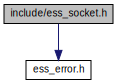
\includegraphics[width=189pt]{df/d02/ess__socket_8h__incl}
\end{center}
\end{figure}
This graph shows which files directly or indirectly include this file\+:
\nopagebreak
\begin{figure}[H]
\begin{center}
\leavevmode
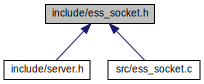
\includegraphics[width=298pt]{de/d4f/ess__socket_8h__dep__incl}
\end{center}
\end{figure}
\subsection*{Data Structures}
\begin{DoxyCompactItemize}
\item 
struct \hyperlink{structess__socket}{ess\+\_\+socket}
\begin{DoxyCompactList}\small\item\em hold all socket managment importend data \end{DoxyCompactList}\end{DoxyCompactItemize}
\subsection*{Typedefs}
\begin{DoxyCompactItemize}
\item 
typedef enum \hyperlink{ess__socket_8h_aeaa282f75f614c7bb033f6b7a72ed037}{ess\+\_\+socket\+\_\+fam} \hyperlink{ess__socket_8h_a9305eae437d57846661e997bb755d150}{ess\+\_\+socket\+\_\+fam\+\_\+t}
\begin{DoxyCompactList}\small\item\em which ip family are use \end{DoxyCompactList}\item 
typedef enum \hyperlink{ess__socket_8h_a2a924f6745a916783fa640cb1c7e1922}{ess\+\_\+socket\+\_\+pro} \hyperlink{ess__socket_8h_a1e8e8de805f8e0b7da25e3b177977273}{ess\+\_\+socket\+\_\+pro\+\_\+t}
\begin{DoxyCompactList}\small\item\em which comunications protocol are use \end{DoxyCompactList}\item 
typedef enum \hyperlink{ess__socket_8h_a85c5abde0574d4a5fbf9e220a18e89dc}{ess\+\_\+socket\+\_\+status} \hyperlink{ess__socket_8h_ae3a6dc482fc34f9ea0361820ba4be573}{ess\+\_\+socket\+\_\+status\+\_\+t}
\begin{DoxyCompactList}\small\item\em \hyperlink{structess__socket}{ess\+\_\+socket} status \end{DoxyCompactList}\item 
typedef struct \hyperlink{structess__socket}{ess\+\_\+socket} \hyperlink{ess__socket_8h_ab7457db5cd500e7f0d74d0bc07356663}{ess\+\_\+socket\+\_\+t}
\begin{DoxyCompactList}\small\item\em hold all socket managment importend data \end{DoxyCompactList}\end{DoxyCompactItemize}
\subsection*{Enumerations}
\begin{DoxyCompactItemize}
\item 
enum \hyperlink{ess__socket_8h_aeaa282f75f614c7bb033f6b7a72ed037}{ess\+\_\+socket\+\_\+fam} \{ \hyperlink{ess__socket_8h_aeaa282f75f614c7bb033f6b7a72ed037a5e2c7645ba65720d7b828d111df09bb1}{E\+S\+S\+\_\+\+S\+O\+C\+K\+E\+T\+\_\+\+F\+A\+M\+I\+L\+Y\+\_\+\+I\+P4}, 
\hyperlink{ess__socket_8h_aeaa282f75f614c7bb033f6b7a72ed037aff947ddfbc0a3d635ad83146dbaa3a72}{E\+S\+S\+\_\+\+S\+O\+C\+K\+E\+T\+\_\+\+F\+A\+M\+I\+L\+Y\+\_\+\+I\+P6}, 
\hyperlink{ess__socket_8h_aeaa282f75f614c7bb033f6b7a72ed037a7376a04481497185206395231d23624d}{E\+S\+S\+\_\+\+S\+O\+C\+K\+E\+T\+\_\+\+F\+A\+M\+I\+L\+Y\+\_\+\+B\+O\+TH}
 \}\begin{DoxyCompactList}\small\item\em which ip family are use \end{DoxyCompactList}
\item 
enum \hyperlink{ess__socket_8h_a2a924f6745a916783fa640cb1c7e1922}{ess\+\_\+socket\+\_\+pro} \{ \hyperlink{ess__socket_8h_a2a924f6745a916783fa640cb1c7e1922a93d8e041d336d1198151ca5cca210d34}{E\+S\+S\+\_\+\+S\+O\+C\+K\+E\+T\+\_\+\+P\+R\+O\+T\+O\+\_\+\+D\+R\+AM}, 
\hyperlink{ess__socket_8h_a2a924f6745a916783fa640cb1c7e1922acba46066923047105db966901c0e8904}{E\+S\+S\+\_\+\+S\+O\+C\+K\+E\+T\+\_\+\+P\+R\+O\+T\+O\+\_\+\+S\+T\+R\+E\+AM}, 
\hyperlink{ess__socket_8h_a2a924f6745a916783fa640cb1c7e1922afb68fe5545329fb828acf269580e0be9}{E\+S\+S\+\_\+\+S\+O\+C\+K\+E\+T\+\_\+\+P\+R\+O\+T\+O\+\_\+\+D\+R\+A\+M\+\_\+\+L\+I\+TE}
 \}\begin{DoxyCompactList}\small\item\em which comunications protocol are use \end{DoxyCompactList}
\item 
enum \hyperlink{ess__socket_8h_a85c5abde0574d4a5fbf9e220a18e89dc}{ess\+\_\+socket\+\_\+status} \{ \newline
\hyperlink{ess__socket_8h_a85c5abde0574d4a5fbf9e220a18e89dca12156322e5e18ca7411b18dba57b9874}{E\+S\+S\+\_\+\+S\+O\+C\+K\+E\+T\+\_\+\+S\+T\+A\+T\+U\+S\+\_\+\+C\+R\+E\+A\+T\+ED}, 
\hyperlink{ess__socket_8h_a85c5abde0574d4a5fbf9e220a18e89dca7ee468f68ee4bd3cfbcdc6bda032be83}{E\+S\+S\+\_\+\+S\+O\+C\+K\+E\+T\+\_\+\+S\+T\+A\+T\+U\+S\+\_\+\+L\+I\+S\+T\+EN}, 
\hyperlink{ess__socket_8h_a85c5abde0574d4a5fbf9e220a18e89dca37cf1e968a55c1fffcf40faa6fe58bd2}{E\+S\+S\+\_\+\+S\+O\+C\+K\+E\+T\+\_\+\+S\+T\+A\+T\+U\+S\+\_\+\+S\+T\+O\+P\+P\+ED}, 
\hyperlink{ess__socket_8h_a85c5abde0574d4a5fbf9e220a18e89dcaa44487507568afb1224527edc59777bc}{E\+S\+S\+\_\+\+S\+O\+C\+K\+E\+T\+\_\+\+S\+T\+A\+T\+U\+S\+\_\+\+E\+R\+R\+OR}, 
\newline
\hyperlink{ess__socket_8h_a85c5abde0574d4a5fbf9e220a18e89dca5af7d3436478f96533b600da6a749ad9}{E\+S\+S\+\_\+\+S\+O\+C\+K\+E\+T\+\_\+\+S\+T\+A\+T\+U\+S\+\_\+\+D\+E\+S\+T\+R\+OY}
 \}\begin{DoxyCompactList}\small\item\em \hyperlink{structess__socket}{ess\+\_\+socket} status \end{DoxyCompactList}
\end{DoxyCompactItemize}
\subsection*{Functions}
\begin{DoxyCompactItemize}
\item 
\hyperlink{ess__socket_8h_a9305eae437d57846661e997bb755d150}{ess\+\_\+socket\+\_\+fam\+\_\+t} \hyperlink{ess__socket_8h_aa50935ade25f18193eae883d52936d35}{ess\+\_\+get\+\_\+address\+\_\+family} (const char $\ast$hostname)
\begin{DoxyCompactList}\small\item\em Look up which address families a host supports. \end{DoxyCompactList}\item 
\hyperlink{ess__error_8h_a08ab97fcf6745dee67de912e41bd3236}{ess\+\_\+error\+\_\+t} \hyperlink{ess__socket_8h_a9a56fb3768b443909f73bb84b7952cb2}{ess\+\_\+socket\+\_\+create\+\_\+server} (\hyperlink{ess__socket_8h_a9305eae437d57846661e997bb755d150}{ess\+\_\+socket\+\_\+fam\+\_\+t} fam, \hyperlink{ess__socket_8h_a1e8e8de805f8e0b7da25e3b177977273}{ess\+\_\+socket\+\_\+pro\+\_\+t} protokoll, const char $\ast$addr, unsigned short port, \hyperlink{ess__socket_8h_ab7457db5cd500e7f0d74d0bc07356663}{ess\+\_\+socket\+\_\+t} $\ast$socket)
\begin{DoxyCompactList}\small\item\em Create a T\+CP or U\+DP server socket. \end{DoxyCompactList}\item 
\hyperlink{ess__socket_8h_ab7457db5cd500e7f0d74d0bc07356663}{ess\+\_\+socket\+\_\+t} $\ast$ \hyperlink{ess__socket_8h_ac205e3a8f4f3786d88d5462ab8847414}{ess\+\_\+socket\+\_\+accept} (\hyperlink{ess__socket_8h_ab7457db5cd500e7f0d74d0bc07356663}{ess\+\_\+socket\+\_\+t} $\ast$server\+\_\+socket, \hyperlink{ess__error_8h_a08ab97fcf6745dee67de912e41bd3236}{ess\+\_\+error\+\_\+t} $\ast$error\+\_\+code)
\begin{DoxyCompactList}\small\item\em accept a connection attempt on a server socket. \end{DoxyCompactList}\item 
\hyperlink{ess__error_8h_a08ab97fcf6745dee67de912e41bd3236}{ess\+\_\+error\+\_\+t} \hyperlink{ess__socket_8h_af007b9ad6c587c0e1c30a2e9fd883da3}{ess\+\_\+socket\+\_\+close} (\hyperlink{ess__socket_8h_ab7457db5cd500e7f0d74d0bc07356663}{ess\+\_\+socket\+\_\+t} $\ast$socket)
\begin{DoxyCompactList}\small\item\em Close a socket. \end{DoxyCompactList}\item 
\hyperlink{ess__error_8h_a08ab97fcf6745dee67de912e41bd3236}{ess\+\_\+error\+\_\+t} \hyperlink{ess__socket_8h_a4e31af0d18cc5b7b5a56de944d2ce62a}{ess\+\_\+socket\+\_\+end\+\_\+write} (\hyperlink{ess__socket_8h_ab7457db5cd500e7f0d74d0bc07356663}{ess\+\_\+socket\+\_\+t} $\ast$socket)
\begin{DoxyCompactList}\small\item\em perform a {\ttfamily shutdown(2)} call on a socket (write) \end{DoxyCompactList}\item 
\hyperlink{ess__error_8h_a08ab97fcf6745dee67de912e41bd3236}{ess\+\_\+error\+\_\+t} \hyperlink{ess__socket_8h_a01a98541c1c0a9d48f96dd8d4d5ac7ac}{ess\+\_\+socket\+\_\+end\+\_\+read} (\hyperlink{ess__socket_8h_ab7457db5cd500e7f0d74d0bc07356663}{ess\+\_\+socket\+\_\+t} $\ast$socket)
\begin{DoxyCompactList}\small\item\em perform a {\ttfamily shutdown(2)} call on a socket (read) \end{DoxyCompactList}\item 
\hyperlink{ess__error_8h_a08ab97fcf6745dee67de912e41bd3236}{ess\+\_\+error\+\_\+t} \hyperlink{ess__socket_8h_a356fa52fcec30125f75ad2fa2e35ef00}{ess\+\_\+socket\+\_\+end} (\hyperlink{ess__socket_8h_ab7457db5cd500e7f0d74d0bc07356663}{ess\+\_\+socket\+\_\+t} $\ast$socket)
\begin{DoxyCompactList}\small\item\em perform a {\ttfamily shutdown(2)} call on a socket (read/write) \end{DoxyCompactList}\item 
\hyperlink{ess__error_8h_a08ab97fcf6745dee67de912e41bd3236}{ess\+\_\+error\+\_\+t} \hyperlink{ess__socket_8h_a0282292df47969a858ca75e94df8b288}{ess\+\_\+socket\+\_\+set\+\_\+buffer} (\hyperlink{ess__socket_8h_ab7457db5cd500e7f0d74d0bc07356663}{ess\+\_\+socket\+\_\+t} $\ast$socket, unsigned int rec\+\_\+buffer\+\_\+size, unsigned int send\+\_\+buffer\+\_\+size)
\begin{DoxyCompactList}\small\item\em set send and recive buffer size of the socket \end{DoxyCompactList}\item 
\hyperlink{ess__socket_8h_ab7457db5cd500e7f0d74d0bc07356663}{ess\+\_\+socket\+\_\+t} $\ast$ \hyperlink{ess__socket_8h_adef36f85812a91bfa3ded44e273d4c18}{ess\+\_\+socket\+\_\+connect\+\_\+stream} (const char $\ast$hostname, int port, \hyperlink{ess__socket_8h_a9305eae437d57846661e997bb755d150}{ess\+\_\+socket\+\_\+fam\+\_\+t} family, int flags, \hyperlink{ess__error_8h_a08ab97fcf6745dee67de912e41bd3236}{ess\+\_\+error\+\_\+t} $\ast$error\+\_\+code)
\begin{DoxyCompactList}\small\item\em Create and connect a new T\+C\+P/\+IP socket. \end{DoxyCompactList}\item 
\hyperlink{ess__socket_8h_ab7457db5cd500e7f0d74d0bc07356663}{ess\+\_\+socket\+\_\+t} $\ast$ \hyperlink{ess__socket_8h_a78d5b3a7daf7c40ab4b3a30ef8205ccc}{ess\+\_\+socket\+\_\+create\+\_\+dram} (\hyperlink{ess__socket_8h_a9305eae437d57846661e997bb755d150}{ess\+\_\+socket\+\_\+fam\+\_\+t} fam, \hyperlink{ess__socket_8h_a1e8e8de805f8e0b7da25e3b177977273}{ess\+\_\+socket\+\_\+pro\+\_\+t} proto, int flags, \hyperlink{ess__error_8h_a08ab97fcf6745dee67de912e41bd3236}{ess\+\_\+error\+\_\+t} $\ast$error\+\_\+code)
\begin{DoxyCompactList}\small\item\em Creates a new U\+D\+P/\+IP socket. \end{DoxyCompactList}\item 
\hyperlink{ess__error_8h_a08ab97fcf6745dee67de912e41bd3236}{ess\+\_\+error\+\_\+t} \hyperlink{ess__socket_8h_a41ea07f9f56e4572955f73f0f237826a}{ess\+\_\+socket\+\_\+connect\+\_\+dram} (\hyperlink{ess__socket_8h_ab7457db5cd500e7f0d74d0bc07356663}{ess\+\_\+socket\+\_\+t} $\ast$socket, const char $\ast$hostname, int port)
\begin{DoxyCompactList}\small\item\em connect a new U\+DP socket \end{DoxyCompactList}\item 
\hyperlink{ess__error_8h_a08ab97fcf6745dee67de912e41bd3236}{ess\+\_\+error\+\_\+t} \hyperlink{ess__socket_8h_a62b826aa7c650a8d4dc447f029364a94}{ess\+\_\+socket\+\_\+write\+\_\+dram} (\hyperlink{ess__socket_8h_ab7457db5cd500e7f0d74d0bc07356663}{ess\+\_\+socket\+\_\+t} $\ast$socket, const void $\ast$buf, unsigned int size, const char $\ast$host, int port, int sendto\+\_\+flags)
\begin{DoxyCompactList}\small\item\em This function is the equivalent to {\ttfamily sendto(2)} \end{DoxyCompactList}\item 
\hyperlink{ess__error_8h_a08ab97fcf6745dee67de912e41bd3236}{ess\+\_\+error\+\_\+t} \hyperlink{ess__socket_8h_abe25e0d1df2293293f0aa3ee0dedadcf}{ess\+\_\+socket\+\_\+read\+\_\+dram} (\hyperlink{ess__socket_8h_ab7457db5cd500e7f0d74d0bc07356663}{ess\+\_\+socket\+\_\+t} $\ast$socket, void $\ast$buf, unsigned int size, char $\ast$src\+\_\+host, unsigned int src\+\_\+host\+\_\+len, int src\+\_\+port, int recvfrom\+\_\+flags)
\begin{DoxyCompactList}\small\item\em Receive data from a U\+D\+P/\+IP socket. \end{DoxyCompactList}\item 
\hyperlink{ess__error_8h_a08ab97fcf6745dee67de912e41bd3236}{ess\+\_\+error\+\_\+t} \hyperlink{ess__socket_8h_a944f0798ea120bef422f97909451b1a9}{ess\+\_\+socket\+\_\+read} (\hyperlink{ess__socket_8h_ab7457db5cd500e7f0d74d0bc07356663}{ess\+\_\+socket\+\_\+t} $\ast$socket, void $\ast$buffer, unsigned int size, unsigned int $\ast$readed)
\begin{DoxyCompactList}\small\item\em read from socket \end{DoxyCompactList}\item 
\hyperlink{ess__error_8h_a08ab97fcf6745dee67de912e41bd3236}{ess\+\_\+error\+\_\+t} \hyperlink{ess__socket_8h_a1cda1ccc6857cde561484dd998124bd7}{ess\+\_\+socket\+\_\+write} (\hyperlink{ess__socket_8h_ab7457db5cd500e7f0d74d0bc07356663}{ess\+\_\+socket\+\_\+t} $\ast$socket, const void $\ast$buffer, unsigned int size, unsigned int $\ast$wrote)
\begin{DoxyCompactList}\small\item\em read from socket \end{DoxyCompactList}\end{DoxyCompactItemize}


\subsection{Typedef Documentation}
\mbox{\Hypertarget{ess__socket_8h_a9305eae437d57846661e997bb755d150}\label{ess__socket_8h_a9305eae437d57846661e997bb755d150}} 
\index{ess\+\_\+socket.\+h@{ess\+\_\+socket.\+h}!ess\+\_\+socket\+\_\+fam\+\_\+t@{ess\+\_\+socket\+\_\+fam\+\_\+t}}
\index{ess\+\_\+socket\+\_\+fam\+\_\+t@{ess\+\_\+socket\+\_\+fam\+\_\+t}!ess\+\_\+socket.\+h@{ess\+\_\+socket.\+h}}
\subsubsection{\texorpdfstring{ess\+\_\+socket\+\_\+fam\+\_\+t}{ess\_socket\_fam\_t}}
{\footnotesize\ttfamily typedef enum \hyperlink{ess__socket_8h_aeaa282f75f614c7bb033f6b7a72ed037}{ess\+\_\+socket\+\_\+fam} \hyperlink{ess__socket_8h_a9305eae437d57846661e997bb755d150}{ess\+\_\+socket\+\_\+fam\+\_\+t}}



which ip family are use 

\mbox{\Hypertarget{ess__socket_8h_a1e8e8de805f8e0b7da25e3b177977273}\label{ess__socket_8h_a1e8e8de805f8e0b7da25e3b177977273}} 
\index{ess\+\_\+socket.\+h@{ess\+\_\+socket.\+h}!ess\+\_\+socket\+\_\+pro\+\_\+t@{ess\+\_\+socket\+\_\+pro\+\_\+t}}
\index{ess\+\_\+socket\+\_\+pro\+\_\+t@{ess\+\_\+socket\+\_\+pro\+\_\+t}!ess\+\_\+socket.\+h@{ess\+\_\+socket.\+h}}
\subsubsection{\texorpdfstring{ess\+\_\+socket\+\_\+pro\+\_\+t}{ess\_socket\_pro\_t}}
{\footnotesize\ttfamily typedef enum \hyperlink{ess__socket_8h_a2a924f6745a916783fa640cb1c7e1922}{ess\+\_\+socket\+\_\+pro} \hyperlink{ess__socket_8h_a1e8e8de805f8e0b7da25e3b177977273}{ess\+\_\+socket\+\_\+pro\+\_\+t}}



which comunications protocol are use 

\mbox{\Hypertarget{ess__socket_8h_ae3a6dc482fc34f9ea0361820ba4be573}\label{ess__socket_8h_ae3a6dc482fc34f9ea0361820ba4be573}} 
\index{ess\+\_\+socket.\+h@{ess\+\_\+socket.\+h}!ess\+\_\+socket\+\_\+status\+\_\+t@{ess\+\_\+socket\+\_\+status\+\_\+t}}
\index{ess\+\_\+socket\+\_\+status\+\_\+t@{ess\+\_\+socket\+\_\+status\+\_\+t}!ess\+\_\+socket.\+h@{ess\+\_\+socket.\+h}}
\subsubsection{\texorpdfstring{ess\+\_\+socket\+\_\+status\+\_\+t}{ess\_socket\_status\_t}}
{\footnotesize\ttfamily typedef enum \hyperlink{ess__socket_8h_a85c5abde0574d4a5fbf9e220a18e89dc}{ess\+\_\+socket\+\_\+status} \hyperlink{ess__socket_8h_ae3a6dc482fc34f9ea0361820ba4be573}{ess\+\_\+socket\+\_\+status\+\_\+t}}



\hyperlink{structess__socket}{ess\+\_\+socket} status 

\mbox{\Hypertarget{ess__socket_8h_ab7457db5cd500e7f0d74d0bc07356663}\label{ess__socket_8h_ab7457db5cd500e7f0d74d0bc07356663}} 
\index{ess\+\_\+socket.\+h@{ess\+\_\+socket.\+h}!ess\+\_\+socket\+\_\+t@{ess\+\_\+socket\+\_\+t}}
\index{ess\+\_\+socket\+\_\+t@{ess\+\_\+socket\+\_\+t}!ess\+\_\+socket.\+h@{ess\+\_\+socket.\+h}}
\subsubsection{\texorpdfstring{ess\+\_\+socket\+\_\+t}{ess\_socket\_t}}
{\footnotesize\ttfamily typedef struct \hyperlink{structess__socket}{ess\+\_\+socket} \hyperlink{ess__socket_8h_ab7457db5cd500e7f0d74d0bc07356663}{ess\+\_\+socket\+\_\+t}}



hold all socket managment importend data 



\subsection{Enumeration Type Documentation}
\mbox{\Hypertarget{ess__socket_8h_aeaa282f75f614c7bb033f6b7a72ed037}\label{ess__socket_8h_aeaa282f75f614c7bb033f6b7a72ed037}} 
\index{ess\+\_\+socket.\+h@{ess\+\_\+socket.\+h}!ess\+\_\+socket\+\_\+fam@{ess\+\_\+socket\+\_\+fam}}
\index{ess\+\_\+socket\+\_\+fam@{ess\+\_\+socket\+\_\+fam}!ess\+\_\+socket.\+h@{ess\+\_\+socket.\+h}}
\subsubsection{\texorpdfstring{ess\+\_\+socket\+\_\+fam}{ess\_socket\_fam}}
{\footnotesize\ttfamily enum \hyperlink{ess__socket_8h_aeaa282f75f614c7bb033f6b7a72ed037}{ess\+\_\+socket\+\_\+fam}}



which ip family are use 

\begin{DoxyEnumFields}{Enumerator}
\raisebox{\heightof{T}}[0pt][0pt]{\index{E\+S\+S\+\_\+\+S\+O\+C\+K\+E\+T\+\_\+\+F\+A\+M\+I\+L\+Y\+\_\+\+I\+P4@{E\+S\+S\+\_\+\+S\+O\+C\+K\+E\+T\+\_\+\+F\+A\+M\+I\+L\+Y\+\_\+\+I\+P4}!ess\+\_\+socket.\+h@{ess\+\_\+socket.\+h}}\index{ess\+\_\+socket.\+h@{ess\+\_\+socket.\+h}!E\+S\+S\+\_\+\+S\+O\+C\+K\+E\+T\+\_\+\+F\+A\+M\+I\+L\+Y\+\_\+\+I\+P4@{E\+S\+S\+\_\+\+S\+O\+C\+K\+E\+T\+\_\+\+F\+A\+M\+I\+L\+Y\+\_\+\+I\+P4}}}\mbox{\Hypertarget{ess__socket_8h_aeaa282f75f614c7bb033f6b7a72ed037a5e2c7645ba65720d7b828d111df09bb1}\label{ess__socket_8h_aeaa282f75f614c7bb033f6b7a72ed037a5e2c7645ba65720d7b828d111df09bb1}} 
E\+S\+S\+\_\+\+S\+O\+C\+K\+E\+T\+\_\+\+F\+A\+M\+I\+L\+Y\+\_\+\+I\+P4&Internet protocol version 4 \\
\hline

\raisebox{\heightof{T}}[0pt][0pt]{\index{E\+S\+S\+\_\+\+S\+O\+C\+K\+E\+T\+\_\+\+F\+A\+M\+I\+L\+Y\+\_\+\+I\+P6@{E\+S\+S\+\_\+\+S\+O\+C\+K\+E\+T\+\_\+\+F\+A\+M\+I\+L\+Y\+\_\+\+I\+P6}!ess\+\_\+socket.\+h@{ess\+\_\+socket.\+h}}\index{ess\+\_\+socket.\+h@{ess\+\_\+socket.\+h}!E\+S\+S\+\_\+\+S\+O\+C\+K\+E\+T\+\_\+\+F\+A\+M\+I\+L\+Y\+\_\+\+I\+P6@{E\+S\+S\+\_\+\+S\+O\+C\+K\+E\+T\+\_\+\+F\+A\+M\+I\+L\+Y\+\_\+\+I\+P6}}}\mbox{\Hypertarget{ess__socket_8h_aeaa282f75f614c7bb033f6b7a72ed037aff947ddfbc0a3d635ad83146dbaa3a72}\label{ess__socket_8h_aeaa282f75f614c7bb033f6b7a72ed037aff947ddfbc0a3d635ad83146dbaa3a72}} 
E\+S\+S\+\_\+\+S\+O\+C\+K\+E\+T\+\_\+\+F\+A\+M\+I\+L\+Y\+\_\+\+I\+P6&Internet protocol version 6 \\
\hline

\raisebox{\heightof{T}}[0pt][0pt]{\index{E\+S\+S\+\_\+\+S\+O\+C\+K\+E\+T\+\_\+\+F\+A\+M\+I\+L\+Y\+\_\+\+B\+O\+TH@{E\+S\+S\+\_\+\+S\+O\+C\+K\+E\+T\+\_\+\+F\+A\+M\+I\+L\+Y\+\_\+\+B\+O\+TH}!ess\+\_\+socket.\+h@{ess\+\_\+socket.\+h}}\index{ess\+\_\+socket.\+h@{ess\+\_\+socket.\+h}!E\+S\+S\+\_\+\+S\+O\+C\+K\+E\+T\+\_\+\+F\+A\+M\+I\+L\+Y\+\_\+\+B\+O\+TH@{E\+S\+S\+\_\+\+S\+O\+C\+K\+E\+T\+\_\+\+F\+A\+M\+I\+L\+Y\+\_\+\+B\+O\+TH}}}\mbox{\Hypertarget{ess__socket_8h_aeaa282f75f614c7bb033f6b7a72ed037a7376a04481497185206395231d23624d}\label{ess__socket_8h_aeaa282f75f614c7bb033f6b7a72ed037a7376a04481497185206395231d23624d}} 
E\+S\+S\+\_\+\+S\+O\+C\+K\+E\+T\+\_\+\+F\+A\+M\+I\+L\+Y\+\_\+\+B\+O\+TH&Unspec D\+NS resolver should decide. \\
\hline

\end{DoxyEnumFields}


Definition at line 38 of file ess\+\_\+socket.\+h.


\begin{DoxyCode}
38                             \{
39   \hyperlink{ess__socket_8h_aeaa282f75f614c7bb033f6b7a72ed037a5e2c7645ba65720d7b828d111df09bb1}{ESS\_SOCKET\_FAMILY\_IP4},       
40   \hyperlink{ess__socket_8h_aeaa282f75f614c7bb033f6b7a72ed037aff947ddfbc0a3d635ad83146dbaa3a72}{ESS\_SOCKET\_FAMILY\_IP6},      
41   \hyperlink{ess__socket_8h_aeaa282f75f614c7bb033f6b7a72ed037a7376a04481497185206395231d23624d}{ESS\_SOCKET\_FAMILY\_BOTH}   
42 \}\hyperlink{ess__socket_8h_a9305eae437d57846661e997bb755d150}{ess\_socket\_fam\_t};
\end{DoxyCode}
\mbox{\Hypertarget{ess__socket_8h_a2a924f6745a916783fa640cb1c7e1922}\label{ess__socket_8h_a2a924f6745a916783fa640cb1c7e1922}} 
\index{ess\+\_\+socket.\+h@{ess\+\_\+socket.\+h}!ess\+\_\+socket\+\_\+pro@{ess\+\_\+socket\+\_\+pro}}
\index{ess\+\_\+socket\+\_\+pro@{ess\+\_\+socket\+\_\+pro}!ess\+\_\+socket.\+h@{ess\+\_\+socket.\+h}}
\subsubsection{\texorpdfstring{ess\+\_\+socket\+\_\+pro}{ess\_socket\_pro}}
{\footnotesize\ttfamily enum \hyperlink{ess__socket_8h_a2a924f6745a916783fa640cb1c7e1922}{ess\+\_\+socket\+\_\+pro}}



which comunications protocol are use 

\begin{DoxyEnumFields}{Enumerator}
\raisebox{\heightof{T}}[0pt][0pt]{\index{E\+S\+S\+\_\+\+S\+O\+C\+K\+E\+T\+\_\+\+P\+R\+O\+T\+O\+\_\+\+D\+R\+AM@{E\+S\+S\+\_\+\+S\+O\+C\+K\+E\+T\+\_\+\+P\+R\+O\+T\+O\+\_\+\+D\+R\+AM}!ess\+\_\+socket.\+h@{ess\+\_\+socket.\+h}}\index{ess\+\_\+socket.\+h@{ess\+\_\+socket.\+h}!E\+S\+S\+\_\+\+S\+O\+C\+K\+E\+T\+\_\+\+P\+R\+O\+T\+O\+\_\+\+D\+R\+AM@{E\+S\+S\+\_\+\+S\+O\+C\+K\+E\+T\+\_\+\+P\+R\+O\+T\+O\+\_\+\+D\+R\+AM}}}\mbox{\Hypertarget{ess__socket_8h_a2a924f6745a916783fa640cb1c7e1922a93d8e041d336d1198151ca5cca210d34}\label{ess__socket_8h_a2a924f6745a916783fa640cb1c7e1922a93d8e041d336d1198151ca5cca210d34}} 
E\+S\+S\+\_\+\+S\+O\+C\+K\+E\+T\+\_\+\+P\+R\+O\+T\+O\+\_\+\+D\+R\+AM&U\+DP \\
\hline

\raisebox{\heightof{T}}[0pt][0pt]{\index{E\+S\+S\+\_\+\+S\+O\+C\+K\+E\+T\+\_\+\+P\+R\+O\+T\+O\+\_\+\+S\+T\+R\+E\+AM@{E\+S\+S\+\_\+\+S\+O\+C\+K\+E\+T\+\_\+\+P\+R\+O\+T\+O\+\_\+\+S\+T\+R\+E\+AM}!ess\+\_\+socket.\+h@{ess\+\_\+socket.\+h}}\index{ess\+\_\+socket.\+h@{ess\+\_\+socket.\+h}!E\+S\+S\+\_\+\+S\+O\+C\+K\+E\+T\+\_\+\+P\+R\+O\+T\+O\+\_\+\+S\+T\+R\+E\+AM@{E\+S\+S\+\_\+\+S\+O\+C\+K\+E\+T\+\_\+\+P\+R\+O\+T\+O\+\_\+\+S\+T\+R\+E\+AM}}}\mbox{\Hypertarget{ess__socket_8h_a2a924f6745a916783fa640cb1c7e1922acba46066923047105db966901c0e8904}\label{ess__socket_8h_a2a924f6745a916783fa640cb1c7e1922acba46066923047105db966901c0e8904}} 
E\+S\+S\+\_\+\+S\+O\+C\+K\+E\+T\+\_\+\+P\+R\+O\+T\+O\+\_\+\+S\+T\+R\+E\+AM&T\+CP \\
\hline

\raisebox{\heightof{T}}[0pt][0pt]{\index{E\+S\+S\+\_\+\+S\+O\+C\+K\+E\+T\+\_\+\+P\+R\+O\+T\+O\+\_\+\+D\+R\+A\+M\+\_\+\+L\+I\+TE@{E\+S\+S\+\_\+\+S\+O\+C\+K\+E\+T\+\_\+\+P\+R\+O\+T\+O\+\_\+\+D\+R\+A\+M\+\_\+\+L\+I\+TE}!ess\+\_\+socket.\+h@{ess\+\_\+socket.\+h}}\index{ess\+\_\+socket.\+h@{ess\+\_\+socket.\+h}!E\+S\+S\+\_\+\+S\+O\+C\+K\+E\+T\+\_\+\+P\+R\+O\+T\+O\+\_\+\+D\+R\+A\+M\+\_\+\+L\+I\+TE@{E\+S\+S\+\_\+\+S\+O\+C\+K\+E\+T\+\_\+\+P\+R\+O\+T\+O\+\_\+\+D\+R\+A\+M\+\_\+\+L\+I\+TE}}}\mbox{\Hypertarget{ess__socket_8h_a2a924f6745a916783fa640cb1c7e1922afb68fe5545329fb828acf269580e0be9}\label{ess__socket_8h_a2a924f6745a916783fa640cb1c7e1922afb68fe5545329fb828acf269580e0be9}} 
E\+S\+S\+\_\+\+S\+O\+C\+K\+E\+T\+\_\+\+P\+R\+O\+T\+O\+\_\+\+D\+R\+A\+M\+\_\+\+L\+I\+TE&U\+DP Lite \\
\hline

\end{DoxyEnumFields}


Definition at line 47 of file ess\+\_\+socket.\+h.


\begin{DoxyCode}
47                             \{
48   \hyperlink{ess__socket_8h_a2a924f6745a916783fa640cb1c7e1922a93d8e041d336d1198151ca5cca210d34}{ESS\_SOCKET\_PROTO\_DRAM},              
49   \hyperlink{ess__socket_8h_a2a924f6745a916783fa640cb1c7e1922acba46066923047105db966901c0e8904}{ESS\_SOCKET\_PROTO\_STREAM},         
50   \hyperlink{ess__socket_8h_a2a924f6745a916783fa640cb1c7e1922afb68fe5545329fb828acf269580e0be9}{ESS\_SOCKET\_PROTO\_DRAM\_LITE}, 
51 \}\hyperlink{ess__socket_8h_a1e8e8de805f8e0b7da25e3b177977273}{ess\_socket\_pro\_t};
\end{DoxyCode}
\mbox{\Hypertarget{ess__socket_8h_a85c5abde0574d4a5fbf9e220a18e89dc}\label{ess__socket_8h_a85c5abde0574d4a5fbf9e220a18e89dc}} 
\index{ess\+\_\+socket.\+h@{ess\+\_\+socket.\+h}!ess\+\_\+socket\+\_\+status@{ess\+\_\+socket\+\_\+status}}
\index{ess\+\_\+socket\+\_\+status@{ess\+\_\+socket\+\_\+status}!ess\+\_\+socket.\+h@{ess\+\_\+socket.\+h}}
\subsubsection{\texorpdfstring{ess\+\_\+socket\+\_\+status}{ess\_socket\_status}}
{\footnotesize\ttfamily enum \hyperlink{ess__socket_8h_a85c5abde0574d4a5fbf9e220a18e89dc}{ess\+\_\+socket\+\_\+status}}



\hyperlink{structess__socket}{ess\+\_\+socket} status 

\begin{DoxyEnumFields}{Enumerator}
\raisebox{\heightof{T}}[0pt][0pt]{\index{E\+S\+S\+\_\+\+S\+O\+C\+K\+E\+T\+\_\+\+S\+T\+A\+T\+U\+S\+\_\+\+C\+R\+E\+A\+T\+ED@{E\+S\+S\+\_\+\+S\+O\+C\+K\+E\+T\+\_\+\+S\+T\+A\+T\+U\+S\+\_\+\+C\+R\+E\+A\+T\+ED}!ess\+\_\+socket.\+h@{ess\+\_\+socket.\+h}}\index{ess\+\_\+socket.\+h@{ess\+\_\+socket.\+h}!E\+S\+S\+\_\+\+S\+O\+C\+K\+E\+T\+\_\+\+S\+T\+A\+T\+U\+S\+\_\+\+C\+R\+E\+A\+T\+ED@{E\+S\+S\+\_\+\+S\+O\+C\+K\+E\+T\+\_\+\+S\+T\+A\+T\+U\+S\+\_\+\+C\+R\+E\+A\+T\+ED}}}\mbox{\Hypertarget{ess__socket_8h_a85c5abde0574d4a5fbf9e220a18e89dca12156322e5e18ca7411b18dba57b9874}\label{ess__socket_8h_a85c5abde0574d4a5fbf9e220a18e89dca12156322e5e18ca7411b18dba57b9874}} 
E\+S\+S\+\_\+\+S\+O\+C\+K\+E\+T\+\_\+\+S\+T\+A\+T\+U\+S\+\_\+\+C\+R\+E\+A\+T\+ED&Socket is created and ready for using \\
\hline

\raisebox{\heightof{T}}[0pt][0pt]{\index{E\+S\+S\+\_\+\+S\+O\+C\+K\+E\+T\+\_\+\+S\+T\+A\+T\+U\+S\+\_\+\+L\+I\+S\+T\+EN@{E\+S\+S\+\_\+\+S\+O\+C\+K\+E\+T\+\_\+\+S\+T\+A\+T\+U\+S\+\_\+\+L\+I\+S\+T\+EN}!ess\+\_\+socket.\+h@{ess\+\_\+socket.\+h}}\index{ess\+\_\+socket.\+h@{ess\+\_\+socket.\+h}!E\+S\+S\+\_\+\+S\+O\+C\+K\+E\+T\+\_\+\+S\+T\+A\+T\+U\+S\+\_\+\+L\+I\+S\+T\+EN@{E\+S\+S\+\_\+\+S\+O\+C\+K\+E\+T\+\_\+\+S\+T\+A\+T\+U\+S\+\_\+\+L\+I\+S\+T\+EN}}}\mbox{\Hypertarget{ess__socket_8h_a85c5abde0574d4a5fbf9e220a18e89dca7ee468f68ee4bd3cfbcdc6bda032be83}\label{ess__socket_8h_a85c5abde0574d4a5fbf9e220a18e89dca7ee468f68ee4bd3cfbcdc6bda032be83}} 
E\+S\+S\+\_\+\+S\+O\+C\+K\+E\+T\+\_\+\+S\+T\+A\+T\+U\+S\+\_\+\+L\+I\+S\+T\+EN&server is running \\
\hline

\raisebox{\heightof{T}}[0pt][0pt]{\index{E\+S\+S\+\_\+\+S\+O\+C\+K\+E\+T\+\_\+\+S\+T\+A\+T\+U\+S\+\_\+\+S\+T\+O\+P\+P\+ED@{E\+S\+S\+\_\+\+S\+O\+C\+K\+E\+T\+\_\+\+S\+T\+A\+T\+U\+S\+\_\+\+S\+T\+O\+P\+P\+ED}!ess\+\_\+socket.\+h@{ess\+\_\+socket.\+h}}\index{ess\+\_\+socket.\+h@{ess\+\_\+socket.\+h}!E\+S\+S\+\_\+\+S\+O\+C\+K\+E\+T\+\_\+\+S\+T\+A\+T\+U\+S\+\_\+\+S\+T\+O\+P\+P\+ED@{E\+S\+S\+\_\+\+S\+O\+C\+K\+E\+T\+\_\+\+S\+T\+A\+T\+U\+S\+\_\+\+S\+T\+O\+P\+P\+ED}}}\mbox{\Hypertarget{ess__socket_8h_a85c5abde0574d4a5fbf9e220a18e89dca37cf1e968a55c1fffcf40faa6fe58bd2}\label{ess__socket_8h_a85c5abde0574d4a5fbf9e220a18e89dca37cf1e968a55c1fffcf40faa6fe58bd2}} 
E\+S\+S\+\_\+\+S\+O\+C\+K\+E\+T\+\_\+\+S\+T\+A\+T\+U\+S\+\_\+\+S\+T\+O\+P\+P\+ED&socket is close \\
\hline

\raisebox{\heightof{T}}[0pt][0pt]{\index{E\+S\+S\+\_\+\+S\+O\+C\+K\+E\+T\+\_\+\+S\+T\+A\+T\+U\+S\+\_\+\+E\+R\+R\+OR@{E\+S\+S\+\_\+\+S\+O\+C\+K\+E\+T\+\_\+\+S\+T\+A\+T\+U\+S\+\_\+\+E\+R\+R\+OR}!ess\+\_\+socket.\+h@{ess\+\_\+socket.\+h}}\index{ess\+\_\+socket.\+h@{ess\+\_\+socket.\+h}!E\+S\+S\+\_\+\+S\+O\+C\+K\+E\+T\+\_\+\+S\+T\+A\+T\+U\+S\+\_\+\+E\+R\+R\+OR@{E\+S\+S\+\_\+\+S\+O\+C\+K\+E\+T\+\_\+\+S\+T\+A\+T\+U\+S\+\_\+\+E\+R\+R\+OR}}}\mbox{\Hypertarget{ess__socket_8h_a85c5abde0574d4a5fbf9e220a18e89dcaa44487507568afb1224527edc59777bc}\label{ess__socket_8h_a85c5abde0574d4a5fbf9e220a18e89dcaa44487507568afb1224527edc59777bc}} 
E\+S\+S\+\_\+\+S\+O\+C\+K\+E\+T\+\_\+\+S\+T\+A\+T\+U\+S\+\_\+\+E\+R\+R\+OR&socket has an error \\
\hline

\raisebox{\heightof{T}}[0pt][0pt]{\index{E\+S\+S\+\_\+\+S\+O\+C\+K\+E\+T\+\_\+\+S\+T\+A\+T\+U\+S\+\_\+\+D\+E\+S\+T\+R\+OY@{E\+S\+S\+\_\+\+S\+O\+C\+K\+E\+T\+\_\+\+S\+T\+A\+T\+U\+S\+\_\+\+D\+E\+S\+T\+R\+OY}!ess\+\_\+socket.\+h@{ess\+\_\+socket.\+h}}\index{ess\+\_\+socket.\+h@{ess\+\_\+socket.\+h}!E\+S\+S\+\_\+\+S\+O\+C\+K\+E\+T\+\_\+\+S\+T\+A\+T\+U\+S\+\_\+\+D\+E\+S\+T\+R\+OY@{E\+S\+S\+\_\+\+S\+O\+C\+K\+E\+T\+\_\+\+S\+T\+A\+T\+U\+S\+\_\+\+D\+E\+S\+T\+R\+OY}}}\mbox{\Hypertarget{ess__socket_8h_a85c5abde0574d4a5fbf9e220a18e89dca5af7d3436478f96533b600da6a749ad9}\label{ess__socket_8h_a85c5abde0574d4a5fbf9e220a18e89dca5af7d3436478f96533b600da6a749ad9}} 
E\+S\+S\+\_\+\+S\+O\+C\+K\+E\+T\+\_\+\+S\+T\+A\+T\+U\+S\+\_\+\+D\+E\+S\+T\+R\+OY&socket is destroyed \\
\hline

\end{DoxyEnumFields}


Definition at line 56 of file ess\+\_\+socket.\+h.


\begin{DoxyCode}
56                                \{
57   \hyperlink{ess__socket_8h_a85c5abde0574d4a5fbf9e220a18e89dca12156322e5e18ca7411b18dba57b9874}{ESS\_SOCKET\_STATUS\_CREATED},    
58   \hyperlink{ess__socket_8h_a85c5abde0574d4a5fbf9e220a18e89dca7ee468f68ee4bd3cfbcdc6bda032be83}{ESS\_SOCKET\_STATUS\_LISTEN},         
59   \hyperlink{ess__socket_8h_a85c5abde0574d4a5fbf9e220a18e89dca37cf1e968a55c1fffcf40faa6fe58bd2}{ESS\_SOCKET\_STATUS\_STOPPED},    
60   \hyperlink{ess__socket_8h_a85c5abde0574d4a5fbf9e220a18e89dcaa44487507568afb1224527edc59777bc}{ESS\_SOCKET\_STATUS\_ERROR},       
61   \hyperlink{ess__socket_8h_a85c5abde0574d4a5fbf9e220a18e89dca5af7d3436478f96533b600da6a749ad9}{ESS\_SOCKET\_STATUS\_DESTROY}   
62 \}\hyperlink{ess__socket_8h_ae3a6dc482fc34f9ea0361820ba4be573}{ess\_socket\_status\_t};
\end{DoxyCode}


\subsection{Function Documentation}
\mbox{\Hypertarget{ess__socket_8h_aa50935ade25f18193eae883d52936d35}\label{ess__socket_8h_aa50935ade25f18193eae883d52936d35}} 
\index{ess\+\_\+socket.\+h@{ess\+\_\+socket.\+h}!ess\+\_\+get\+\_\+address\+\_\+family@{ess\+\_\+get\+\_\+address\+\_\+family}}
\index{ess\+\_\+get\+\_\+address\+\_\+family@{ess\+\_\+get\+\_\+address\+\_\+family}!ess\+\_\+socket.\+h@{ess\+\_\+socket.\+h}}
\subsubsection{\texorpdfstring{ess\+\_\+get\+\_\+address\+\_\+family()}{ess\_get\_address\_family()}}
{\footnotesize\ttfamily \hyperlink{ess__socket_8h_a9305eae437d57846661e997bb755d150}{ess\+\_\+socket\+\_\+fam\+\_\+t} ess\+\_\+get\+\_\+address\+\_\+family (\begin{DoxyParamCaption}\item[{const char $\ast$}]{hostname }\end{DoxyParamCaption})}



Look up which address families a host supports. 

If you want to send a datagram to a host but you don\textquotesingle{}t know if it supports I\+Pv4 or I\+Pv6, use this function.


\begin{DoxyParams}{Parameters}
{\em hostname} & The hostname of the host you want to look up.\\
\hline
\end{DoxyParams}

\begin{DoxyRetVals}{Return values}
{\em E\+S\+S\+\_\+\+S\+O\+C\+K\+E\+T\+\_\+\+F\+A\+M\+I\+L\+Y\+\_\+\+I\+P4} & Host supports only I\+P4 \\
\hline
{\em E\+S\+S\+\_\+\+S\+O\+C\+K\+E\+T\+\_\+\+F\+A\+M\+I\+L\+Y\+\_\+\+I\+P6} & Host supports I\+P6 and I\+P4 \\
\hline
{\em $<$0} & Error. \\
\hline
\end{DoxyRetVals}


Definition at line 47 of file ess\+\_\+socket.\+c.


\begin{DoxyCode}
47                                                               \{
48   \hyperlink{ess__socket_8h_a9305eae437d57846661e997bb755d150}{ess\_socket\_fam\_t} return\_value = -1;
49   \textcolor{keyword}{struct }addrinfo hint, *result;
50   \textcolor{keywordtype}{int} af = -1;
51 
52   \textcolor{keywordflow}{if} ( hostname == NULL ) \textcolor{keywordflow}{return} -1;
53   memset(&hint,0,\textcolor{keyword}{sizeof} hint);
54   hint.ai\_family = AF\_UNSPEC;
55 
56   \textcolor{keywordflow}{if} ( 0 != (return\_value = getaddrinfo(hostname,\textcolor{stringliteral}{"0"},&hint,&result)))   \textcolor{keywordflow}{return} -1;
57   \textcolor{keywordflow}{if} ( result == NULL ) \textcolor{keywordflow}{return} -1;
58 
59   \textcolor{keywordflow}{switch} (result->ai\_family) \{
60     \textcolor{keywordflow}{case} AF\_INET:   af = \hyperlink{ess__socket_8h_aeaa282f75f614c7bb033f6b7a72ed037a5e2c7645ba65720d7b828d111df09bb1}{ESS\_SOCKET\_FAMILY\_IP4}; \textcolor{keywordflow}{break};
61     \textcolor{keywordflow}{case} AF\_INET6: af= \hyperlink{ess__socket_8h_aeaa282f75f614c7bb033f6b7a72ed037aff947ddfbc0a3d635ad83146dbaa3a72}{ESS\_SOCKET\_FAMILY\_IP6}; \textcolor{keywordflow}{break};
62   \};
63   \textcolor{keywordflow}{return} af;
64 \}
\end{DoxyCode}
\mbox{\Hypertarget{ess__socket_8h_ac205e3a8f4f3786d88d5462ab8847414}\label{ess__socket_8h_ac205e3a8f4f3786d88d5462ab8847414}} 
\index{ess\+\_\+socket.\+h@{ess\+\_\+socket.\+h}!ess\+\_\+socket\+\_\+accept@{ess\+\_\+socket\+\_\+accept}}
\index{ess\+\_\+socket\+\_\+accept@{ess\+\_\+socket\+\_\+accept}!ess\+\_\+socket.\+h@{ess\+\_\+socket.\+h}}
\subsubsection{\texorpdfstring{ess\+\_\+socket\+\_\+accept()}{ess\_socket\_accept()}}
{\footnotesize\ttfamily \hyperlink{ess__socket_8h_ab7457db5cd500e7f0d74d0bc07356663}{ess\+\_\+socket\+\_\+t}$\ast$ ess\+\_\+socket\+\_\+accept (\begin{DoxyParamCaption}\item[{\hyperlink{ess__socket_8h_ab7457db5cd500e7f0d74d0bc07356663}{ess\+\_\+socket\+\_\+t} $\ast$}]{server\+\_\+socket,  }\item[{\hyperlink{ess__error_8h_a08ab97fcf6745dee67de912e41bd3236}{ess\+\_\+error\+\_\+t} $\ast$}]{error\+\_\+code }\end{DoxyParamCaption})}



accept a connection attempt on a server socket. 

This function accepts an incoming connection on a server socket.


\begin{DoxyParams}{Parameters}
{\em server\+\_\+socket} & the server socket \\
\hline
{\em error\+\_\+code} & \\
\hline
\end{DoxyParams}

\begin{DoxyRetVals}{Return values}
{\em !=} & 0 A the client socket \\
\hline
{\em N\+U\+LL} & Error see paramerter \textquotesingle{}error\+\_\+code\textquotesingle{} \\
\hline
\end{DoxyRetVals}


Definition at line 180 of file ess\+\_\+socket.\+c.


\begin{DoxyCode}
180                                                                                       \{
181   \textcolor{keywordflow}{if}(server\_socket == 0) \{ \textcolor{keywordflow}{if}(error\_code != 0) *error\_code = \hyperlink{ess__error_8h_a3a40ffb47f45a17c8989af8286e7a07fa96978468215ef7117c99232e72d7fb39}{ESS\_ERROR\_NULL}; \textcolor{keywordflow}{return} 0; \}
182 
183   \hyperlink{structess__socket}{ess\_socket\_t} *client\_socket;
184   \textcolor{keywordtype}{int}  nbl = 0;
185   \textcolor{keyword}{struct }sockaddr\_in incoming;
186   \textcolor{keyword}{struct }sockaddr\_in6 incoming6;
187   \textcolor{keywordtype}{unsigned} \textcolor{keywordtype}{int} size\_in6 = \textcolor{keyword}{sizeof}(\textcolor{keyword}{struct }sockaddr\_in6);
188   \textcolor{keywordtype}{unsigned} \textcolor{keywordtype}{int} size\_in = \textcolor{keyword}{sizeof}(\textcolor{keyword}{struct }sockaddr\_in);
189 
190   \textcolor{comment}{//socklen\_t addrlen = sizeof(struct sockaddr\_storage);}
191 
192 
193   client\_socket = (\hyperlink{structess__socket}{ess\_socket\_t}*)malloc(\textcolor{keyword}{sizeof}(\hyperlink{structess__socket}{ess\_socket\_t}));
194   \textcolor{keywordflow}{if}(client\_socket == 0) \textcolor{keywordflow}{return} 0;
195 
196   client\_socket->\hyperlink{structess__socket_a4d0d74743d167680649419163ce8c80e}{hostname\_len} = INET6\_ADDRSTRLEN;
197 
198   \textcolor{keywordflow}{if}(server\_socket->\hyperlink{structess__socket_ad09623d57ebd33fef8dac4e18c0cba2f}{family} == \hyperlink{ess__socket_8h_aeaa282f75f614c7bb033f6b7a72ed037a5e2c7645ba65720d7b828d111df09bb1}{ESS\_SOCKET\_FAMILY\_IP4}) \{
199 
200     \textcolor{keywordflow}{if} ( (client\_socket->\hyperlink{structess__socket_a3666576f6b88007cc7b8f26c7da596c8}{socket} = accept(server\_socket->\hyperlink{structess__socket_a3666576f6b88007cc7b8f26c7da596c8}{socket}, (\textcolor{keyword}{struct} sockaddr*)&incoming, (
      socklen\_t *) &size\_in)) != 0) \{
201       \textcolor{keywordflow}{if}(error\_code != 0) *error\_code = \hyperlink{ess__error_8h_a3a40ffb47f45a17c8989af8286e7a07fa96978468215ef7117c99232e72d7fb39}{ESS\_ERROR\_NULL};
202       \textcolor{keywordflow}{return} 0;
203     \}
204 
205     \textcolor{keywordflow}{if}(server\_socket->\hyperlink{structess__socket_a1f0429596710512357072b192ba3d2bd}{protokol} == \hyperlink{ess__socket_8h_a2a924f6745a916783fa640cb1c7e1922acba46066923047105db966901c0e8904}{ESS\_SOCKET\_PROTO\_STREAM}) \{
206       server\_socket->\hyperlink{structess__socket_a938bdc6ae46c346147b6d4f67ad1e704}{port}  = ntohs( incoming.sin\_port );
207           \textcolor{keywordtype}{long} addr = ntohl( incoming.sin\_addr.s\_addr );
208 
209       client\_socket->\hyperlink{structess__socket_a0c6be700c8763c26054098348ebef8d6}{hostname}[0] = \textcolor{charliteral}{'\(\backslash\)0'};
210       snprintf(client\_socket->\hyperlink{structess__socket_a0c6be700c8763c26054098348ebef8d6}{hostname},  client\_socket->\hyperlink{structess__socket_a4d0d74743d167680649419163ce8c80e}{hostname\_len}, \textcolor{stringliteral}{"
      %03u.%03u.%03u.%03u"},
211         (\textcolor{keywordtype}{unsigned} \textcolor{keywordtype}{int}) addr >> 24,  (\textcolor{keywordtype}{unsigned} \textcolor{keywordtype}{int}) (addr >> 16) % 256,  (\textcolor{keywordtype}{unsigned} \textcolor{keywordtype}{int}) (addr >> 8) % 256,
212         (\textcolor{keywordtype}{unsigned} \textcolor{keywordtype}{int}) addr % 256 );
213       client\_socket->\hyperlink{structess__socket_a4d0d74743d167680649419163ce8c80e}{hostname\_len} = strlen(client\_socket->\hyperlink{structess__socket_a0c6be700c8763c26054098348ebef8d6}{hostname});
214     \}
215 
216   \} \textcolor{keywordflow}{else} \{
217 
218     \textcolor{keywordflow}{if} ( (client\_socket->\hyperlink{structess__socket_a3666576f6b88007cc7b8f26c7da596c8}{socket} = accept( server\_socket->\hyperlink{structess__socket_a3666576f6b88007cc7b8f26c7da596c8}{socket},(\textcolor{keyword}{struct} sockaddr *)&incoming6, 
      (socklen\_t *) &size\_in6 )) != 0) \{
219       \textcolor{keywordflow}{if}(error\_code != 0) *error\_code = \hyperlink{ess__error_8h_a3a40ffb47f45a17c8989af8286e7a07fa96978468215ef7117c99232e72d7fb39}{ESS\_ERROR\_NULL};
220       \textcolor{keywordflow}{return} 0;
221     \}
222 
223     \textcolor{keywordtype}{char} addrbuf[INET6\_ADDRSTRLEN];
224     addrbuf[0] = \textcolor{charliteral}{'\(\backslash\)0'};
225 
226     client\_socket->\hyperlink{structess__socket_a938bdc6ae46c346147b6d4f67ad1e704}{port} = ntohs( incoming6.sin6\_port );
227 
228     \textcolor{keywordflow}{if} ( inet\_ntop( AF\_INET6, &(incoming6.sin6\_addr), addrbuf, \textcolor{keyword}{sizeof}(addrbuf) )) \{
229       ESP\_LOGI(\textcolor{stringliteral}{"EssS"}, \textcolor{stringliteral}{"client from :%s/%d"}, addrbuf, client\_socket->\hyperlink{structess__socket_a938bdc6ae46c346147b6d4f67ad1e704}{port});
230       client\_socket->\hyperlink{structess__socket_a0c6be700c8763c26054098348ebef8d6}{hostname}[0] = \textcolor{charliteral}{'\(\backslash\)0'};
231       strncpy(client\_socket->\hyperlink{structess__socket_a0c6be700c8763c26054098348ebef8d6}{hostname},  addrbuf,  strlen(addrbuf) );
232     \}
233   \}
234 
235   \textcolor{keywordflow}{if} ( ioctl( client\_socket->\hyperlink{structess__socket_a3666576f6b88007cc7b8f26c7da596c8}{socket} , FIONBIO, &nbl ) < 0 ) \{
236     ESP\_LOGE(\textcolor{stringliteral}{"EssS"}, \textcolor{stringliteral}{"(%02d) couldn't turn on blocking for client"},  client\_socket->
      \hyperlink{structess__socket_a3666576f6b88007cc7b8f26c7da596c8}{socket} );
237     client\_socket->\hyperlink{structess__socket_a4e47521e8af756b9edf77f1f02f9b725}{status} = \hyperlink{ess__socket_8h_a85c5abde0574d4a5fbf9e220a18e89dcaa44487507568afb1224527edc59777bc}{ESS\_SOCKET\_STATUS\_ERROR};
238     \textcolor{keywordflow}{if}(error\_code != 0) \{ *error\_code = \hyperlink{ess__error_8h_a3a40ffb47f45a17c8989af8286e7a07fa96978468215ef7117c99232e72d7fb39}{ESS\_ERROR\_NULL}; \textcolor{keywordflow}{return} 0; \}
239 
240     close(client\_socket->\hyperlink{structess__socket_a3666576f6b88007cc7b8f26c7da596c8}{socket});
241   \}
242   \textcolor{keywordflow}{return} client\_socket;
243 \}
\end{DoxyCode}
\mbox{\Hypertarget{ess__socket_8h_af007b9ad6c587c0e1c30a2e9fd883da3}\label{ess__socket_8h_af007b9ad6c587c0e1c30a2e9fd883da3}} 
\index{ess\+\_\+socket.\+h@{ess\+\_\+socket.\+h}!ess\+\_\+socket\+\_\+close@{ess\+\_\+socket\+\_\+close}}
\index{ess\+\_\+socket\+\_\+close@{ess\+\_\+socket\+\_\+close}!ess\+\_\+socket.\+h@{ess\+\_\+socket.\+h}}
\subsubsection{\texorpdfstring{ess\+\_\+socket\+\_\+close()}{ess\_socket\_close()}}
{\footnotesize\ttfamily \hyperlink{ess__error_8h_a08ab97fcf6745dee67de912e41bd3236}{ess\+\_\+error\+\_\+t} ess\+\_\+socket\+\_\+close (\begin{DoxyParamCaption}\item[{\hyperlink{ess__socket_8h_ab7457db5cd500e7f0d74d0bc07356663}{ess\+\_\+socket\+\_\+t} $\ast$}]{socket }\end{DoxyParamCaption})}



Close a socket. 

This function closes a socket.


\begin{DoxyParams}{Parameters}
{\em socket} & the using socket struct\\
\hline
\end{DoxyParams}

\begin{DoxyRetVals}{Return values}
{\em E\+S\+S\+\_\+\+OK} & Closed socket successfully \\
\hline
{\em E\+S\+S\+\_\+\+E\+R\+R\+O\+R\+\_\+\+N\+U\+LL} & socket was N\+U\+LL \\
\hline
{\em E\+S\+S\+\_\+\+E\+R\+R\+O\+R\+\_\+\+C\+L\+O\+SE} & Socket was already closed (other errors are very unlikely to occur) \\
\hline
\end{DoxyRetVals}


Definition at line 130 of file ess\+\_\+socket.\+c.


\begin{DoxyCode}
130                                                     \{
131   \textcolor{keywordflow}{if}(\_socket == 0) \textcolor{keywordflow}{return} \hyperlink{ess__error_8h_a3a40ffb47f45a17c8989af8286e7a07fa96978468215ef7117c99232e72d7fb39}{ESS\_ERROR\_NULL};
132 
133   \textcolor{keywordflow}{if} (  (\_socket->retval  = close(\_socket->socket))  != 0 ) \{
134     \_socket->status = \hyperlink{ess__socket_8h_a85c5abde0574d4a5fbf9e220a18e89dcaa44487507568afb1224527edc59777bc}{ESS\_SOCKET\_STATUS\_ERROR};
135     \textcolor{keywordflow}{return} \hyperlink{ess__error_8h_a3a40ffb47f45a17c8989af8286e7a07fa3c103cfeedd28b98ed4c47427b1b69ca}{ESS\_ERROR\_CLOSE};
136   \}
137   \textcolor{keywordflow}{return} \hyperlink{ess__error_8h_a3a40ffb47f45a17c8989af8286e7a07fa7a39eb24d172b29cca7678967088d864}{ESS\_OK};
138 \}
\end{DoxyCode}
\mbox{\Hypertarget{ess__socket_8h_a41ea07f9f56e4572955f73f0f237826a}\label{ess__socket_8h_a41ea07f9f56e4572955f73f0f237826a}} 
\index{ess\+\_\+socket.\+h@{ess\+\_\+socket.\+h}!ess\+\_\+socket\+\_\+connect\+\_\+dram@{ess\+\_\+socket\+\_\+connect\+\_\+dram}}
\index{ess\+\_\+socket\+\_\+connect\+\_\+dram@{ess\+\_\+socket\+\_\+connect\+\_\+dram}!ess\+\_\+socket.\+h@{ess\+\_\+socket.\+h}}
\subsubsection{\texorpdfstring{ess\+\_\+socket\+\_\+connect\+\_\+dram()}{ess\_socket\_connect\_dram()}}
{\footnotesize\ttfamily \hyperlink{ess__error_8h_a08ab97fcf6745dee67de912e41bd3236}{ess\+\_\+error\+\_\+t} ess\+\_\+socket\+\_\+connect\+\_\+dram (\begin{DoxyParamCaption}\item[{\hyperlink{ess__socket_8h_ab7457db5cd500e7f0d74d0bc07356663}{ess\+\_\+socket\+\_\+t} $\ast$}]{socket,  }\item[{const char $\ast$}]{hostname,  }\item[{int}]{port }\end{DoxyParamCaption})}



connect a new U\+DP socket 

This function returns a working client U\+DP socket.


\begin{DoxyParams}{Parameters}
{\em hostname} & The host the socket will be connected to (everything resolvable, e.\+g. \char`\"{}\+::1\char`\"{}, \char`\"{}8.\+8.\+8.\+8\char`\"{}, \char`\"{}example.\+com\char`\"{}) \\
\hline
{\em port} & The host\textquotesingle{}s port. \\
\hline
{\em family} & {\ttfamily E\+S\+S\+\_\+\+S\+O\+C\+K\+E\+T\+\_\+\+F\+A\+M\+I\+L\+Y\+\_\+\+I\+P6} or {\ttfamily E\+S\+S\+\_\+\+S\+O\+C\+K\+E\+T\+\_\+\+F\+A\+M\+I\+L\+Y\+\_\+\+I\+P4}. \\
\hline
{\em prot} & {\ttfamily E\+S\+S\+\_\+\+S\+O\+C\+K\+E\+T\+\_\+\+P\+R\+O\+T\+O\+\_\+\+D\+R\+AM} or {\ttfamily E\+S\+S\+\_\+\+S\+O\+C\+K\+E\+T\+\_\+\+P\+R\+O\+T\+O\+\_\+\+D\+R\+A\+M\+\_\+\+L\+I\+TE} \\
\hline
{\em error\+\_\+code} & E\+S\+S\+\_\+\+E\+R\+R\+O\+R\+\_\+\+N\+U\+LL hostname was N\+U\+LL\\
\hline
\end{DoxyParams}

\begin{DoxyRetVals}{Return values}
{\em N\+U\+LL} & Error see paramerter \textquotesingle{}error\+\_\+code\textquotesingle{} \\
\hline
\end{DoxyRetVals}
\begin{DoxyReturn}{Returns}
A valid socket. 
\end{DoxyReturn}


Definition at line 356 of file ess\+\_\+socket.\+c.


\begin{DoxyCode}
356                                                                                         \{
357 
358   \textcolor{keyword}{struct }addrinfo *result, *result\_check, hint;
359   \textcolor{keyword}{struct }sockaddr\_storage oldsockaddr;
360   socklen\_t oldsockaddrlen = \textcolor{keyword}{sizeof}(\textcolor{keyword}{struct }sockaddr\_storage);
361   \textcolor{keywordtype}{char} buffer[8]; buffer[0] = \textcolor{charliteral}{'\(\backslash\)0'};
362 
363 
364   snprintf(buffer, 8,\textcolor{stringliteral}{"%d"},port) ;
365 
366   \textcolor{keywordflow}{if} ( host == NULL ) \{
367     \textcolor{keywordflow}{return} 0;
368   \}
369 
370   \textcolor{comment}{//TODO: Create new ERROR Codes}
371 
372   \textcolor{keywordflow}{if} ( -1 == getsockname(\_socket->socket,(\textcolor{keyword}{struct} sockaddr*)&oldsockaddr,&oldsockaddrlen) )\{
373     \textcolor{keywordflow}{return} \hyperlink{ess__error_8h_a3a40ffb47f45a17c8989af8286e7a07faa28e2c57627994f0cfa08dd3b4e28b97}{ESS\_ERROR};
374   \}
375 
376   \textcolor{keywordflow}{if} ( oldsockaddrlen > \textcolor{keyword}{sizeof}(\textcolor{keyword}{struct} sockaddr\_storage) ) \{
377     \textcolor{keywordflow}{return} \hyperlink{ess__error_8h_a3a40ffb47f45a17c8989af8286e7a07faa28e2c57627994f0cfa08dd3b4e28b97}{ESS\_ERROR};
378   \}
379 
380   memset(&hint,0,\textcolor{keyword}{sizeof}(\textcolor{keyword}{struct} addrinfo));
381 
382   hint.ai\_family = ((\textcolor{keyword}{struct }sockaddr\_in*)&oldsockaddr)->sin\_family; \textcolor{comment}{// AF\_INET or AF\_INET6 - offset is same
       at sockaddr\_in and sockaddr\_in6}
383 
384   hint.ai\_socktype =  SOCK\_DGRAM;
385 
386   \textcolor{keywordflow}{if} (  getaddrinfo(host,buffer,&hint,&result) != 0) \{
387     \textcolor{keywordflow}{return} \hyperlink{ess__error_8h_a3a40ffb47f45a17c8989af8286e7a07fa27d1d29e5376284759ed12c811b4d94e}{ESS\_ERROR\_GETADDR};
388   \}
389 
390   \textcolor{keywordflow}{for} ( result\_check = result; result\_check != NULL; result\_check = result\_check->ai\_next ) \{ \textcolor{comment}{// go through
       the linked list of struct addrinfo elements}
391     \textcolor{keywordflow}{if} (  connect(\_socket->socket,result\_check->ai\_addr,result\_check->ai\_addrlen) != -1) \textcolor{comment}{// connected
       without error}
392         \textcolor{keywordflow}{break};
393 
394     \textcolor{keywordflow}{if} ( result\_check == 0 ) \{
395       \textcolor{keywordflow}{return} \hyperlink{ess__error_8h_a3a40ffb47f45a17c8989af8286e7a07faa30baabd6fe0c3ccddb08d1692308f0e}{ESS\_ERROR\_CONNECT};
396     \}
397   \}
398   freeaddrinfo(result);
399 
400   \_socket->hostname\_len = strlen(host);
401   strncpy(\_socket->hostname, host, \_socket->hostname\_len);
402   \_socket->port = port;
403 
404   \textcolor{keywordflow}{return} \hyperlink{ess__error_8h_a3a40ffb47f45a17c8989af8286e7a07fa7a39eb24d172b29cca7678967088d864}{ESS\_OK};
405 \}
\end{DoxyCode}
\mbox{\Hypertarget{ess__socket_8h_adef36f85812a91bfa3ded44e273d4c18}\label{ess__socket_8h_adef36f85812a91bfa3ded44e273d4c18}} 
\index{ess\+\_\+socket.\+h@{ess\+\_\+socket.\+h}!ess\+\_\+socket\+\_\+connect\+\_\+stream@{ess\+\_\+socket\+\_\+connect\+\_\+stream}}
\index{ess\+\_\+socket\+\_\+connect\+\_\+stream@{ess\+\_\+socket\+\_\+connect\+\_\+stream}!ess\+\_\+socket.\+h@{ess\+\_\+socket.\+h}}
\subsubsection{\texorpdfstring{ess\+\_\+socket\+\_\+connect\+\_\+stream()}{ess\_socket\_connect\_stream()}}
{\footnotesize\ttfamily \hyperlink{ess__socket_8h_ab7457db5cd500e7f0d74d0bc07356663}{ess\+\_\+socket\+\_\+t}$\ast$ ess\+\_\+socket\+\_\+connect\+\_\+stream (\begin{DoxyParamCaption}\item[{const char $\ast$}]{hostname,  }\item[{int}]{port,  }\item[{\hyperlink{ess__socket_8h_a9305eae437d57846661e997bb755d150}{ess\+\_\+socket\+\_\+fam\+\_\+t}}]{family,  }\item[{int}]{flags,  }\item[{\hyperlink{ess__error_8h_a08ab97fcf6745dee67de912e41bd3236}{ess\+\_\+error\+\_\+t} $\ast$}]{error\+\_\+code }\end{DoxyParamCaption})}



Create and connect a new T\+C\+P/\+IP socket. 

This function returns a working client T\+C\+P/\+IP socket.


\begin{DoxyParams}{Parameters}
{\em hostname} & The host the socket will be connected to (everything resolvable, e.\+g. \char`\"{}\+::1\char`\"{}, \char`\"{}8.\+8.\+8.\+8\char`\"{}, \char`\"{}example.\+com\char`\"{}) \\
\hline
{\em port} & The host\textquotesingle{}s port. \\
\hline
{\em family} & {\ttfamily E\+S\+S\+\_\+\+S\+O\+C\+K\+E\+T\+\_\+\+F\+A\+M\+I\+L\+Y\+\_\+\+I\+P6} or {\ttfamily E\+S\+S\+\_\+\+S\+O\+C\+K\+E\+T\+\_\+\+F\+A\+M\+I\+L\+Y\+\_\+\+I\+P4}. \\
\hline
{\em flags} & Flags to be passed to {\ttfamily socket(2)}. Most flags are Linux-\/only! \\
\hline
{\em error\+\_\+code} & E\+S\+S\+\_\+\+E\+R\+R\+O\+R\+\_\+\+N\+U\+LL hostname was N\+U\+LL\\
\hline
\end{DoxyParams}

\begin{DoxyRetVals}{Return values}
{\em N\+U\+LL} & Error see paramerter \textquotesingle{}error\+\_\+code\textquotesingle{} \\
\hline
\end{DoxyRetVals}
\begin{DoxyReturn}{Returns}
A valid socket. 
\end{DoxyReturn}


Definition at line 252 of file ess\+\_\+socket.\+c.


\begin{DoxyCode}
252                                                                                                            
                                 \{
253   \textcolor{keywordflow}{if}(hostname == NULL) \{ \textcolor{keywordflow}{if}(error\_code != 0) \{ *error\_code = \hyperlink{ess__error_8h_a3a40ffb47f45a17c8989af8286e7a07fa96978468215ef7117c99232e72d7fb39}{ESS\_ERROR\_NULL}; \} \textcolor{keywordflow}{return} 0; \}
254 
255   \textcolor{keywordtype}{int} sfd;
256   \textcolor{keyword}{struct }addrinfo hint, *result, *result\_check;
257   \hyperlink{structess__socket}{ess\_socket\_t}* new\_socket;
258   \textcolor{keywordtype}{char} buffer[8]; buffer[0] = \textcolor{charliteral}{'\(\backslash\)0'};
259 
260   memset(&hint,0,\textcolor{keyword}{sizeof} hint);
261 
262   \textcolor{keywordflow}{switch} ( family ) \{
263     \textcolor{keywordflow}{case} \hyperlink{ess__socket_8h_aeaa282f75f614c7bb033f6b7a72ed037a5e2c7645ba65720d7b828d111df09bb1}{ESS\_SOCKET\_FAMILY\_IP4}: hint.ai\_family = AF\_INET; \textcolor{keywordflow}{break};
264     \textcolor{keywordflow}{case} \hyperlink{ess__socket_8h_aeaa282f75f614c7bb033f6b7a72ed037aff947ddfbc0a3d635ad83146dbaa3a72}{ESS\_SOCKET\_FAMILY\_IP6}: hint.ai\_family = AF\_INET6; \textcolor{keywordflow}{break};
265     \textcolor{keywordflow}{default}: hint.ai\_family = AF\_UNSPEC;
266   \}
267 
268 
269   hint.ai\_socktype = SOCK\_STREAM;
270 
271 
272   snprintf(buffer, 8,\textcolor{stringliteral}{"%d"},port) ;
273 
274   \textcolor{keywordflow}{if} (   getaddrinfo(hostname,buffer,&hint,&result) != 0) \{
275     \textcolor{keywordflow}{if}(error\_code != 0) \{ *error\_code = \hyperlink{ess__error_8h_a3a40ffb47f45a17c8989af8286e7a07fa27d1d29e5376284759ed12c811b4d94e}{ESS\_ERROR\_GETADDR}; \}
276     \textcolor{keywordflow}{return} 0;
277   \}
278 
279   \textcolor{keywordflow}{for} ( result\_check = result; result\_check != 0; result\_check = result\_check->ai\_next )  \{ \textcolor{comment}{// go through
       the linked list of struct addrinfo elements}
280       sfd = socket(result\_check->ai\_family, result\_check->ai\_socktype | flags, result\_check->ai\_protocol);
281 
282       \textcolor{keywordflow}{if} ( sfd < 0 )  \textcolor{keywordflow}{continue};
283 
284       \textcolor{keywordflow}{if} (  connect(sfd,result\_check->ai\_addr,result\_check->ai\_addrlen)  != -1) \textcolor{comment}{// connected without error}
285         \textcolor{keywordflow}{break};
286         close(sfd);
287   \}
288   freeaddrinfo(result);
289 
290   \textcolor{keywordflow}{if} ( result\_check == 0 ) \{
291     \textcolor{keywordflow}{if}(error\_code != 0) \{ *error\_code = \hyperlink{ess__error_8h_a3a40ffb47f45a17c8989af8286e7a07fa27d1d29e5376284759ed12c811b4d94e}{ESS\_ERROR\_GETADDR}; \}
292     \textcolor{keywordflow}{return} 0;
293   \}
294   \textcolor{comment}{// Yes :)}
295   new\_socket = (\hyperlink{structess__socket}{ess\_socket\_t}*)malloc(\textcolor{keyword}{sizeof}(\hyperlink{structess__socket}{ess\_socket\_t}));
296   \textcolor{keywordflow}{if}(new\_socket == 0) \{
297     \textcolor{keywordflow}{if}(error\_code != 0) \{ *error\_code = \hyperlink{ess__error_8h_a3a40ffb47f45a17c8989af8286e7a07fa6a45eefc15738cbbc15b5ef516da1c69}{ESS\_ERROR\_OUTOFMEM}; \}
298     \textcolor{keywordflow}{return} 0;
299   \}
300   new\_socket->\hyperlink{structess__socket_a3666576f6b88007cc7b8f26c7da596c8}{socket} = sfd;
301 
302   strncpy(new\_socket->\hyperlink{structess__socket_a0c6be700c8763c26054098348ebef8d6}{hostname}, hostname, strlen(hostname));
303 
304   new\_socket->\hyperlink{structess__socket_a938bdc6ae46c346147b6d4f67ad1e704}{port} = port;
305   new\_socket->\hyperlink{structess__socket_ad09623d57ebd33fef8dac4e18c0cba2f}{family} = family;
306   new\_socket->\hyperlink{structess__socket_a1f0429596710512357072b192ba3d2bd}{protokol} = \hyperlink{ess__socket_8h_a2a924f6745a916783fa640cb1c7e1922acba46066923047105db966901c0e8904}{ESS\_SOCKET\_PROTO\_STREAM};
307 
308   \textcolor{keywordflow}{return} new\_socket;
309 \}
\end{DoxyCode}
\mbox{\Hypertarget{ess__socket_8h_a78d5b3a7daf7c40ab4b3a30ef8205ccc}\label{ess__socket_8h_a78d5b3a7daf7c40ab4b3a30ef8205ccc}} 
\index{ess\+\_\+socket.\+h@{ess\+\_\+socket.\+h}!ess\+\_\+socket\+\_\+create\+\_\+dram@{ess\+\_\+socket\+\_\+create\+\_\+dram}}
\index{ess\+\_\+socket\+\_\+create\+\_\+dram@{ess\+\_\+socket\+\_\+create\+\_\+dram}!ess\+\_\+socket.\+h@{ess\+\_\+socket.\+h}}
\subsubsection{\texorpdfstring{ess\+\_\+socket\+\_\+create\+\_\+dram()}{ess\_socket\_create\_dram()}}
{\footnotesize\ttfamily \hyperlink{ess__socket_8h_ab7457db5cd500e7f0d74d0bc07356663}{ess\+\_\+socket\+\_\+t}$\ast$ ess\+\_\+socket\+\_\+create\+\_\+dram (\begin{DoxyParamCaption}\item[{\hyperlink{ess__socket_8h_a9305eae437d57846661e997bb755d150}{ess\+\_\+socket\+\_\+fam\+\_\+t}}]{fam,  }\item[{\hyperlink{ess__socket_8h_a1e8e8de805f8e0b7da25e3b177977273}{ess\+\_\+socket\+\_\+pro\+\_\+t}}]{proto,  }\item[{int}]{flags,  }\item[{\hyperlink{ess__error_8h_a08ab97fcf6745dee67de912e41bd3236}{ess\+\_\+error\+\_\+t} $\ast$}]{error\+\_\+code }\end{DoxyParamCaption})}



Creates a new U\+D\+P/\+IP socket. 

The socket is automatically bound to some port.


\begin{DoxyParams}[1]{Parameters}
\mbox{\tt in}  & {\em fam} & is E\+S\+S\+\_\+\+S\+O\+C\+K\+E\+T\+\_\+\+F\+A\+M\+I\+L\+Y\+\_\+\+I\+P4 (A\+F\+\_\+\+I\+N\+ET) or E\+S\+S\+\_\+\+S\+O\+C\+K\+E\+T\+\_\+\+F\+A\+M\+I\+L\+Y\+\_\+\+I\+P6 (A\+F\+\_\+\+I\+N\+E\+T6). \\
\hline
\mbox{\tt in}  & {\em proto} & is E\+S\+S\+\_\+\+S\+O\+C\+K\+E\+T\+\_\+\+P\+R\+O\+T\+O\+\_\+\+D\+R\+AM or E\+S\+S\+\_\+\+S\+O\+C\+K\+E\+T\+\_\+\+P\+R\+O\+T\+O\+\_\+\+D\+R\+A\+M\+\_\+\+L\+I\+TE \\
\hline
\mbox{\tt in}  & {\em flags} & may be the flags specified in socket(2), i.\+e. S\+O\+C\+K\+\_\+\+N\+O\+N\+B\+L\+O\+CK and/or S\+O\+C\+K\+\_\+\+C\+L\+O\+E\+X\+EC. More than one flags may be O\+Red. This argument is only sensible on Linux $>$= 2.\+6.\+27! \\
\hline
\mbox{\tt out}  & {\em error\+\_\+code} & if !=0 then error codes\\
\hline
\end{DoxyParams}
\begin{DoxyReturn}{Returns}
The socket file descriptor number, on error N\+U\+LL.
\end{DoxyReturn}
To send and receive data with this socket use the functions explained below, \hyperlink{ess__socket_8h_abe25e0d1df2293293f0aa3ee0dedadcf}{ess\+\_\+socket\+\_\+read\+\_\+dram()} and \hyperlink{ess__socket_8h_a62b826aa7c650a8d4dc447f029364a94}{ess\+\_\+socket\+\_\+write\+\_\+dram()}. 

Definition at line 310 of file ess\+\_\+socket.\+c.


\begin{DoxyCode}
310                                                                                                            
                   \{
311   \textcolor{keywordtype}{int} sfd;
312   \textcolor{keywordtype}{int} \_proto;
313 
314   \textcolor{keywordflow}{if} (fam != \hyperlink{ess__socket_8h_aeaa282f75f614c7bb033f6b7a72ed037aff947ddfbc0a3d635ad83146dbaa3a72}{ESS\_SOCKET\_FAMILY\_IP6} && fam != 
      \hyperlink{ess__socket_8h_aeaa282f75f614c7bb033f6b7a72ed037a5e2c7645ba65720d7b828d111df09bb1}{ESS\_SOCKET\_FAMILY\_IP4})   \{
315     \textcolor{keywordflow}{if}(error\_code != 0) \{ *error\_code = \hyperlink{ess__error_8h_a3a40ffb47f45a17c8989af8286e7a07fa33645fb11bd8e70afa78f70c8510353b}{ESS\_ERROR\_UNSPEC\_FAMILY}; \}
316     \textcolor{keywordflow}{return} 0;
317   \}
318   \textcolor{keywordflow}{if}(proto == \hyperlink{ess__socket_8h_a2a924f6745a916783fa640cb1c7e1922afb68fe5545329fb828acf269580e0be9}{ESS\_SOCKET\_PROTO\_DRAM\_LITE}) \{
319     \_proto = IPPROTO\_UDPLITE;
320   \} \textcolor{keywordflow}{else} \textcolor{keywordflow}{if}(proto == \hyperlink{ess__socket_8h_a2a924f6745a916783fa640cb1c7e1922a93d8e041d336d1198151ca5cca210d34}{ESS\_SOCKET\_PROTO\_DRAM}) \{
321     \_proto  = 0;
322   \} \textcolor{keywordflow}{else} \{
323     \textcolor{keywordflow}{if}(error\_code != 0) \{ *error\_code = \hyperlink{ess__error_8h_a3a40ffb47f45a17c8989af8286e7a07fa6e5f6a4817d742aaf08c97977006bd40}{ESS\_ERROR\_UNSPEC\_PROTOKOL}; \}
324     \textcolor{keywordflow}{return} 0;
325   \}
326 
327   \textcolor{keywordflow}{switch} ( proto )
328   \{
329   \textcolor{keywordflow}{case} \hyperlink{ess__socket_8h_aeaa282f75f614c7bb033f6b7a72ed037a5e2c7645ba65720d7b828d111df09bb1}{ESS\_SOCKET\_FAMILY\_IP4} :
330     sfd = socket(AF\_INET,SOCK\_DGRAM|flags,\_proto);
331     \textcolor{keywordflow}{break};
332   \textcolor{keywordflow}{case} \hyperlink{ess__socket_8h_aeaa282f75f614c7bb033f6b7a72ed037aff947ddfbc0a3d635ad83146dbaa3a72}{ESS\_SOCKET\_FAMILY\_IP6} :
333     sfd = socket(AF\_INET6,SOCK\_DGRAM|flags,\_proto);
334     \textcolor{keywordflow}{break};
335   \textcolor{keywordflow}{default}:
336     \textcolor{keywordflow}{if}(error\_code != 0) \{ *error\_code = \hyperlink{ess__error_8h_a3a40ffb47f45a17c8989af8286e7a07fa33645fb11bd8e70afa78f70c8510353b}{ESS\_ERROR\_UNSPEC\_FAMILY}; \}
337     \textcolor{keywordflow}{return} 0;
338   \}
339 
340   \textcolor{keywordflow}{if} ( -1 == sfd ) \{
341     \textcolor{keywordflow}{if}(error\_code != 0) \{ *error\_code = \hyperlink{ess__error_8h_a3a40ffb47f45a17c8989af8286e7a07faa30baabd6fe0c3ccddb08d1692308f0e}{ESS\_ERROR\_CONNECT}; \}
342     \textcolor{keywordflow}{return} 0;
343   \}
344   \hyperlink{structess__socket}{ess\_socket\_t}*  new\_socket = (\hyperlink{structess__socket}{ess\_socket\_t}*)malloc(\textcolor{keyword}{sizeof}(
      \hyperlink{structess__socket}{ess\_socket\_t}));
345   \textcolor{keywordflow}{if}(new\_socket == 0) \{
346     \textcolor{keywordflow}{if}(error\_code != 0) \{ *error\_code = \hyperlink{ess__error_8h_a3a40ffb47f45a17c8989af8286e7a07fa6a45eefc15738cbbc15b5ef516da1c69}{ESS\_ERROR\_OUTOFMEM}; \}
347     \textcolor{keywordflow}{return} 0;
348   \}
349   new\_socket->\hyperlink{structess__socket_a3666576f6b88007cc7b8f26c7da596c8}{socket} = sfd;
350   new\_socket->\hyperlink{structess__socket_ad09623d57ebd33fef8dac4e18c0cba2f}{family} = fam;
351   new\_socket->\hyperlink{structess__socket_a1f0429596710512357072b192ba3d2bd}{protokol} = proto;
352 
353   \textcolor{keywordflow}{return} new\_socket;
354 \}
\end{DoxyCode}
\mbox{\Hypertarget{ess__socket_8h_a9a56fb3768b443909f73bb84b7952cb2}\label{ess__socket_8h_a9a56fb3768b443909f73bb84b7952cb2}} 
\index{ess\+\_\+socket.\+h@{ess\+\_\+socket.\+h}!ess\+\_\+socket\+\_\+create\+\_\+server@{ess\+\_\+socket\+\_\+create\+\_\+server}}
\index{ess\+\_\+socket\+\_\+create\+\_\+server@{ess\+\_\+socket\+\_\+create\+\_\+server}!ess\+\_\+socket.\+h@{ess\+\_\+socket.\+h}}
\subsubsection{\texorpdfstring{ess\+\_\+socket\+\_\+create\+\_\+server()}{ess\_socket\_create\_server()}}
{\footnotesize\ttfamily \hyperlink{ess__error_8h_a08ab97fcf6745dee67de912e41bd3236}{ess\+\_\+error\+\_\+t} ess\+\_\+socket\+\_\+create\+\_\+server (\begin{DoxyParamCaption}\item[{\hyperlink{ess__socket_8h_a9305eae437d57846661e997bb755d150}{ess\+\_\+socket\+\_\+fam\+\_\+t}}]{fam,  }\item[{\hyperlink{ess__socket_8h_a1e8e8de805f8e0b7da25e3b177977273}{ess\+\_\+socket\+\_\+pro\+\_\+t}}]{protokoll,  }\item[{const char $\ast$}]{addr,  }\item[{unsigned short}]{port,  }\item[{\hyperlink{ess__socket_8h_ab7457db5cd500e7f0d74d0bc07356663}{ess\+\_\+socket\+\_\+t} $\ast$}]{socket }\end{DoxyParamCaption})}



Create a T\+CP or U\+DP server socket. 


\begin{DoxyParams}{Parameters}
{\em protokoll} & {\ttfamily E\+S\+S\+\_\+\+S\+O\+C\+K\+E\+T\+\_\+\+P\+R\+O\+T\+O\+\_\+\+S\+T\+R\+E\+AM}, {\ttfamily E\+S\+S\+\_\+\+S\+O\+C\+K\+E\+T\+\_\+\+P\+R\+O\+T\+O\+\_\+\+D\+R\+AM} or {\ttfamily E\+S\+S\+\_\+\+S\+O\+C\+K\+E\+T\+\_\+\+P\+R\+O\+T\+O\+\_\+\+D\+R\+A\+M\+\_\+\+L\+I\+TE} \\
\hline
{\em fam} & Either {\ttfamily E\+S\+S\+\_\+\+S\+O\+C\+K\+E\+T\+\_\+\+F\+A\+M\+I\+L\+Y\+\_\+\+I\+P4}, {\ttfamily E\+S\+S\+\_\+\+S\+O\+C\+K\+E\+T\+\_\+\+F\+A\+M\+I\+L\+Y\+\_\+\+I\+P6} or {\ttfamily E\+S\+S\+\_\+\+S\+O\+C\+K\+E\+T\+\_\+\+F\+A\+M\+I\+L\+Y\+\_\+\+B\+O\+TH}; latter means that the D\+NS resolver should decide. \\
\hline
{\em bind\+\_\+addr} & Address to bind to. If you want to bind to every address use \char`\"{}0.\+0.\+0.\+0\char`\"{} or \char`\"{}\+::\char`\"{} (I\+Pv6 wildcard) \\
\hline
{\em port} & The port to bind to. \\
\hline
{\em socket} & the using socket struct\\
\hline
\end{DoxyParams}

\begin{DoxyRetVals}{Return values}
{\em E\+S\+S\+\_\+\+OK} & the socket was created -\/ T\+CP socket are listin \\
\hline
{\em E\+S\+S\+\_\+\+E\+R\+R\+O\+R\+\_\+\+U\+N\+S\+P\+EC} & socket alwas created \\
\hline
{\em E\+S\+S\+\_\+\+E\+R\+R\+O\+R\+\_\+\+U\+N\+S\+P\+E\+C\+\_\+\+P\+R\+O\+T\+O\+K\+OL} & unknown protokol  E\+S\+S\+\_\+\+E\+R\+R\+O\+R\+\_\+\+U\+N\+S\+P\+E\+C\+\_\+\+F\+A\+M\+I\+LY unknown family \\
\hline
{\em E\+S\+S\+\_\+\+E\+R\+R\+O\+R\+\_\+\+G\+E\+T\+A\+D\+DR} & \\
\hline
{\em E\+S\+S\+\_\+\+E\+R\+R\+O\+R\+\_\+\+B\+I\+ND} & error to call bind \\
\hline
{\em E\+S\+S\+\_\+\+E\+R\+R\+O\+R\+\_\+\+N\+U\+LL} & socket was N\+U\+LL \\
\hline
\end{DoxyRetVals}


Definition at line 65 of file ess\+\_\+socket.\+c.


\begin{DoxyCode}
66                                                                                                            
                          \{
67   \textcolor{keywordflow}{if}(\_socket == 0) \textcolor{keywordflow}{return} \hyperlink{ess__error_8h_a3a40ffb47f45a17c8989af8286e7a07fa96978468215ef7117c99232e72d7fb39}{ESS\_ERROR\_NULL};
68   \textcolor{keywordflow}{if}( \_socket->status == \hyperlink{ess__socket_8h_a85c5abde0574d4a5fbf9e220a18e89dca37cf1e968a55c1fffcf40faa6fe58bd2}{ESS\_SOCKET\_STATUS\_STOPPED})
69     \textcolor{keywordflow}{return} \hyperlink{ess__error_8h_a3a40ffb47f45a17c8989af8286e7a07faa28e2c57627994f0cfa08dd3b4e28b97}{ESS\_ERROR};
70 
71   \_socket->family = fam;
72   \_socket->protokol = protokoll;
73   \_socket->port = port;
74   \_socket->status = \hyperlink{ess__socket_8h_a85c5abde0574d4a5fbf9e220a18e89dca12156322e5e18ca7411b18dba57b9874}{ESS\_SOCKET\_STATUS\_CREATED};
75   \_socket->hostname[0] = \textcolor{charliteral}{'\(\backslash\)0'};
76   \_socket->hostname\_len = strlen(hostname);
77 
78     strncpy(\_socket->hostname, hostname, strlen(hostname));
79 
80 
81   \textcolor{keyword}{struct }addrinfo *result, *result\_check, hints;
82   memset(&hints,0,\textcolor{keyword}{sizeof}(\textcolor{keyword}{struct} addrinfo));
83 
84   \textcolor{keywordflow}{switch}(\_socket->protokol) \{
85     \textcolor{keywordflow}{case} \hyperlink{ess__socket_8h_a2a924f6745a916783fa640cb1c7e1922acba46066923047105db966901c0e8904}{ESS\_SOCKET\_PROTO\_STREAM}:  hints.ai\_socktype = SOCK\_STREAM;  \textcolor{keywordflow}{break};
86     \textcolor{keywordflow}{case} \hyperlink{ess__socket_8h_a2a924f6745a916783fa640cb1c7e1922a93d8e041d336d1198151ca5cca210d34}{ESS\_SOCKET\_PROTO\_DRAM}:  hints.ai\_socktype = SOCK\_DGRAM; \textcolor{keywordflow}{break};
87     \textcolor{keywordflow}{case} \hyperlink{ess__socket_8h_a2a924f6745a916783fa640cb1c7e1922afb68fe5545329fb828acf269580e0be9}{ESS\_SOCKET\_PROTO\_DRAM\_LITE}:  hints.ai\_socktype = SOCK\_DGRAM;  hints.
      ai\_protocol = IPPROTO\_UDPLITE; \textcolor{keywordflow}{break};
88     \textcolor{keywordflow}{default}: \_socket->status = \hyperlink{ess__socket_8h_a85c5abde0574d4a5fbf9e220a18e89dcaa44487507568afb1224527edc59777bc}{ESS\_SOCKET\_STATUS\_ERROR}; \textcolor{keywordflow}{return} 
      \hyperlink{ess__error_8h_a3a40ffb47f45a17c8989af8286e7a07fa6e5f6a4817d742aaf08c97977006bd40}{ESS\_ERROR\_UNSPEC\_PROTOKOL};
89   \};
90   \textcolor{keywordflow}{switch} ( \_socket->family ) \{
91     \textcolor{keywordflow}{case} \hyperlink{ess__socket_8h_aeaa282f75f614c7bb033f6b7a72ed037a5e2c7645ba65720d7b828d111df09bb1}{ESS\_SOCKET\_FAMILY\_IP4}: hints.ai\_family = AF\_INET; \textcolor{keywordflow}{break};
92     \textcolor{keywordflow}{case} \hyperlink{ess__socket_8h_aeaa282f75f614c7bb033f6b7a72ed037aff947ddfbc0a3d635ad83146dbaa3a72}{ESS\_SOCKET\_FAMILY\_IP6}: hints.ai\_family = AF\_INET6; \textcolor{keywordflow}{break};
93     \textcolor{keywordflow}{case} \hyperlink{ess__socket_8h_aeaa282f75f614c7bb033f6b7a72ed037a7376a04481497185206395231d23624d}{ESS\_SOCKET\_FAMILY\_BOTH}: hints.ai\_family = AF\_UNSPEC; \textcolor{keywordflow}{break};
94     \textcolor{keywordflow}{default}: \_socket->status = \hyperlink{ess__socket_8h_a85c5abde0574d4a5fbf9e220a18e89dcaa44487507568afb1224527edc59777bc}{ESS\_SOCKET\_STATUS\_ERROR}; \textcolor{keywordflow}{return} 
      \hyperlink{ess__error_8h_a3a40ffb47f45a17c8989af8286e7a07fa33645fb11bd8e70afa78f70c8510353b}{ESS\_ERROR\_UNSPEC\_FAMILY};
95   \}
96   hints.ai\_flags = AI\_PASSIVE;
97 
98   \textcolor{keywordtype}{char} buffer[8]; buffer[0] = \textcolor{charliteral}{'\(\backslash\)0'};
99   snprintf(buffer, 8,\textcolor{stringliteral}{"%d"},\_socket->port) ;
100   \textcolor{keywordflow}{if} (  (\_socket->retval = getaddrinfo(\_socket->hostname, buffer ,&hints,&result)) != 0 ) \{
101     \_socket->status = \hyperlink{ess__socket_8h_a85c5abde0574d4a5fbf9e220a18e89dcaa44487507568afb1224527edc59777bc}{ESS\_SOCKET\_STATUS\_ERROR};
102     \textcolor{keywordflow}{return} \hyperlink{ess__error_8h_a3a40ffb47f45a17c8989af8286e7a07fa27d1d29e5376284759ed12c811b4d94e}{ESS\_ERROR\_GETADDR};
103   \}
104 
105   \textcolor{keywordflow}{for} ( result\_check = result; result\_check != NULL; result\_check = result\_check->ai\_next ) \{
106     \_socket->socket = socket(result\_check->ai\_family, result\_check->ai\_socktype, result\_check->ai\_protocol)
      ;
107     \textcolor{keywordflow}{if} ( \_socket->socket < 0 )  \textcolor{keywordflow}{continue};
108     \textcolor{keywordflow}{if} (  (\_socket->retval  = bind(\_socket->socket, result\_check->ai\_addr,(socklen\_t)result\_check->
      ai\_addrlen)) != 0 ) \{
109       close(\_socket->socket); \textcolor{keywordflow}{continue};
110     \}
111     \textcolor{keywordflow}{if} (\_socket->protokol == \hyperlink{ess__socket_8h_a2a924f6745a916783fa640cb1c7e1922acba46066923047105db966901c0e8904}{ESS\_SOCKET\_PROTO\_STREAM}) \{
112         \textcolor{keywordflow}{if} (  (\_socket->retval  = listen(\_socket->socket, 128)) == 0) \{
113           \textcolor{keywordflow}{break};
114         \} \textcolor{keywordflow}{else} \{
115           close(\_socket->socket);
116         \}
117     \}
118   \}
119   \textcolor{keywordflow}{if} ( result\_check == NULL ) \{
120     freeaddrinfo(result);
121     \_socket->status = \hyperlink{ess__socket_8h_a85c5abde0574d4a5fbf9e220a18e89dcaa44487507568afb1224527edc59777bc}{ESS\_SOCKET\_STATUS\_ERROR};
122     \textcolor{keywordflow}{return} \hyperlink{ess__error_8h_a3a40ffb47f45a17c8989af8286e7a07fa497475ae748b432dea8df5daabc4f0ad}{ESS\_ERROR\_BIND};
123   \}
124   freeaddrinfo(result);
125 
126   \_socket->status = \hyperlink{ess__socket_8h_a85c5abde0574d4a5fbf9e220a18e89dca7ee468f68ee4bd3cfbcdc6bda032be83}{ESS\_SOCKET\_STATUS\_LISTEN};
127   \textcolor{keywordflow}{return} \hyperlink{ess__error_8h_a3a40ffb47f45a17c8989af8286e7a07fa7a39eb24d172b29cca7678967088d864}{ESS\_OK};
128 \}
\end{DoxyCode}
Here is the caller graph for this function\+:
\nopagebreak
\begin{figure}[H]
\begin{center}
\leavevmode
\includegraphics[width=336pt]{d8/da1/ess__socket_8h_a9a56fb3768b443909f73bb84b7952cb2_icgraph}
\end{center}
\end{figure}
\mbox{\Hypertarget{ess__socket_8h_a356fa52fcec30125f75ad2fa2e35ef00}\label{ess__socket_8h_a356fa52fcec30125f75ad2fa2e35ef00}} 
\index{ess\+\_\+socket.\+h@{ess\+\_\+socket.\+h}!ess\+\_\+socket\+\_\+end@{ess\+\_\+socket\+\_\+end}}
\index{ess\+\_\+socket\+\_\+end@{ess\+\_\+socket\+\_\+end}!ess\+\_\+socket.\+h@{ess\+\_\+socket.\+h}}
\subsubsection{\texorpdfstring{ess\+\_\+socket\+\_\+end()}{ess\_socket\_end()}}
{\footnotesize\ttfamily \hyperlink{ess__error_8h_a08ab97fcf6745dee67de912e41bd3236}{ess\+\_\+error\+\_\+t} ess\+\_\+socket\+\_\+end (\begin{DoxyParamCaption}\item[{\hyperlink{ess__socket_8h_ab7457db5cd500e7f0d74d0bc07356663}{ess\+\_\+socket\+\_\+t} $\ast$}]{socket }\end{DoxyParamCaption})}



perform a {\ttfamily shutdown(2)} call on a socket (read/write) 


\begin{DoxyParams}{Parameters}
{\em socket} & the using socket struct\\
\hline
\end{DoxyParams}

\begin{DoxyRetVals}{Return values}
{\em E\+S\+S\+\_\+\+OK} & Closed socket successfully \\
\hline
{\em E\+S\+S\+\_\+\+E\+R\+R\+O\+R\+\_\+\+N\+U\+LL} & socket was N\+U\+LL \\
\hline
{\em E\+S\+S\+\_\+\+E\+R\+R\+O\+R\+\_\+\+C\+L\+O\+SE} & Socket was already closed (other errors are very unlikely to occur) \\
\hline
\end{DoxyRetVals}


Definition at line 165 of file ess\+\_\+socket.\+c.


\begin{DoxyCode}
165                                                   \{
166   \textcolor{keywordflow}{if}(\_socket == 0) \textcolor{keywordflow}{return} \hyperlink{ess__error_8h_a3a40ffb47f45a17c8989af8286e7a07fa96978468215ef7117c99232e72d7fb39}{ESS\_ERROR\_NULL};
167 
168   \textcolor{keywordflow}{if} (  (\_socket->retval  = shutdown(\_socket->socket,  SHUT\_RD) )  != 0 ) \{
169     \_socket->status = \hyperlink{ess__socket_8h_a85c5abde0574d4a5fbf9e220a18e89dcaa44487507568afb1224527edc59777bc}{ESS\_SOCKET\_STATUS\_ERROR};
170     \textcolor{keywordflow}{return} \hyperlink{ess__error_8h_a3a40ffb47f45a17c8989af8286e7a07fa3c103cfeedd28b98ed4c47427b1b69ca}{ESS\_ERROR\_CLOSE};
171   \}
172   \textcolor{keywordflow}{if} (  (\_socket->retval  = shutdown(\_socket->socket,  SHUT\_WR) )  != 0 ) \{
173     \_socket->status = \hyperlink{ess__socket_8h_a85c5abde0574d4a5fbf9e220a18e89dcaa44487507568afb1224527edc59777bc}{ESS\_SOCKET\_STATUS\_ERROR};
174     \textcolor{keywordflow}{return} \hyperlink{ess__error_8h_a3a40ffb47f45a17c8989af8286e7a07fa3c103cfeedd28b98ed4c47427b1b69ca}{ESS\_ERROR\_CLOSE};
175   \}
176 
177   \textcolor{keywordflow}{return} \hyperlink{ess__error_8h_a3a40ffb47f45a17c8989af8286e7a07fa7a39eb24d172b29cca7678967088d864}{ESS\_OK};
178 \}
\end{DoxyCode}
\mbox{\Hypertarget{ess__socket_8h_a01a98541c1c0a9d48f96dd8d4d5ac7ac}\label{ess__socket_8h_a01a98541c1c0a9d48f96dd8d4d5ac7ac}} 
\index{ess\+\_\+socket.\+h@{ess\+\_\+socket.\+h}!ess\+\_\+socket\+\_\+end\+\_\+read@{ess\+\_\+socket\+\_\+end\+\_\+read}}
\index{ess\+\_\+socket\+\_\+end\+\_\+read@{ess\+\_\+socket\+\_\+end\+\_\+read}!ess\+\_\+socket.\+h@{ess\+\_\+socket.\+h}}
\subsubsection{\texorpdfstring{ess\+\_\+socket\+\_\+end\+\_\+read()}{ess\_socket\_end\_read()}}
{\footnotesize\ttfamily \hyperlink{ess__error_8h_a08ab97fcf6745dee67de912e41bd3236}{ess\+\_\+error\+\_\+t} ess\+\_\+socket\+\_\+end\+\_\+read (\begin{DoxyParamCaption}\item[{\hyperlink{ess__socket_8h_ab7457db5cd500e7f0d74d0bc07356663}{ess\+\_\+socket\+\_\+t} $\ast$}]{socket }\end{DoxyParamCaption})}



perform a {\ttfamily shutdown(2)} call on a socket (read) 


\begin{DoxyParams}{Parameters}
{\em socket} & the using socket struct\\
\hline
\end{DoxyParams}

\begin{DoxyRetVals}{Return values}
{\em E\+S\+S\+\_\+\+OK} & Closed socket successfully \\
\hline
{\em E\+S\+S\+\_\+\+E\+R\+R\+O\+R\+\_\+\+N\+U\+LL} & socket was N\+U\+LL \\
\hline
{\em E\+S\+S\+\_\+\+E\+R\+R\+O\+R\+\_\+\+C\+L\+O\+SE} & Socket was already closed (other errors are very unlikely to occur) \\
\hline
\end{DoxyRetVals}


Definition at line 155 of file ess\+\_\+socket.\+c.


\begin{DoxyCode}
155                                                        \{
156   \textcolor{keywordflow}{if}(\_socket == 0) \textcolor{keywordflow}{return} \hyperlink{ess__error_8h_a3a40ffb47f45a17c8989af8286e7a07fa96978468215ef7117c99232e72d7fb39}{ESS\_ERROR\_NULL};
157 
158   \textcolor{keywordflow}{if} (  (\_socket->retval  = shutdown(\_socket->socket,  SHUT\_RD) )  != 0 ) \{
159     \_socket->status = \hyperlink{ess__socket_8h_a85c5abde0574d4a5fbf9e220a18e89dcaa44487507568afb1224527edc59777bc}{ESS\_SOCKET\_STATUS\_ERROR};
160     \textcolor{keywordflow}{return} \hyperlink{ess__error_8h_a3a40ffb47f45a17c8989af8286e7a07fa3c103cfeedd28b98ed4c47427b1b69ca}{ESS\_ERROR\_CLOSE};
161   \}
162   \textcolor{keywordflow}{return} \hyperlink{ess__error_8h_a3a40ffb47f45a17c8989af8286e7a07fa7a39eb24d172b29cca7678967088d864}{ESS\_OK};
163 \}
\end{DoxyCode}
\mbox{\Hypertarget{ess__socket_8h_a4e31af0d18cc5b7b5a56de944d2ce62a}\label{ess__socket_8h_a4e31af0d18cc5b7b5a56de944d2ce62a}} 
\index{ess\+\_\+socket.\+h@{ess\+\_\+socket.\+h}!ess\+\_\+socket\+\_\+end\+\_\+write@{ess\+\_\+socket\+\_\+end\+\_\+write}}
\index{ess\+\_\+socket\+\_\+end\+\_\+write@{ess\+\_\+socket\+\_\+end\+\_\+write}!ess\+\_\+socket.\+h@{ess\+\_\+socket.\+h}}
\subsubsection{\texorpdfstring{ess\+\_\+socket\+\_\+end\+\_\+write()}{ess\_socket\_end\_write()}}
{\footnotesize\ttfamily \hyperlink{ess__error_8h_a08ab97fcf6745dee67de912e41bd3236}{ess\+\_\+error\+\_\+t} ess\+\_\+socket\+\_\+end\+\_\+write (\begin{DoxyParamCaption}\item[{\hyperlink{ess__socket_8h_ab7457db5cd500e7f0d74d0bc07356663}{ess\+\_\+socket\+\_\+t} $\ast$}]{socket }\end{DoxyParamCaption})}



perform a {\ttfamily shutdown(2)} call on a socket (write) 

This function closes a socket.


\begin{DoxyParams}{Parameters}
{\em socket} & the using socket struct\\
\hline
\end{DoxyParams}

\begin{DoxyRetVals}{Return values}
{\em E\+S\+S\+\_\+\+OK} & Closed socket successfully \\
\hline
{\em E\+S\+S\+\_\+\+E\+R\+R\+O\+R\+\_\+\+N\+U\+LL} & socket was N\+U\+LL \\
\hline
{\em E\+S\+S\+\_\+\+E\+R\+R\+O\+R\+\_\+\+C\+L\+O\+SE} & Socket was already closed (other errors are very unlikely to occur) \\
\hline
\end{DoxyRetVals}


Definition at line 140 of file ess\+\_\+socket.\+c.


\begin{DoxyCode}
140                                                         \{
141   \textcolor{keywordflow}{if}(\_socket == 0) \textcolor{keywordflow}{return} \hyperlink{ess__error_8h_a3a40ffb47f45a17c8989af8286e7a07fa96978468215ef7117c99232e72d7fb39}{ESS\_ERROR\_NULL};
142 
143   \textcolor{keywordflow}{if} (  (\_socket->retval  = shutdown(\_socket->socket,  SHUT\_WR) )  != 0 ) \{
144     \_socket->status = \hyperlink{ess__socket_8h_a85c5abde0574d4a5fbf9e220a18e89dcaa44487507568afb1224527edc59777bc}{ESS\_SOCKET\_STATUS\_ERROR};
145     \textcolor{keywordflow}{return} \hyperlink{ess__error_8h_a3a40ffb47f45a17c8989af8286e7a07fa3c103cfeedd28b98ed4c47427b1b69ca}{ESS\_ERROR\_CLOSE};
146   \}
147   \textcolor{keywordflow}{return} \hyperlink{ess__error_8h_a3a40ffb47f45a17c8989af8286e7a07fa7a39eb24d172b29cca7678967088d864}{ESS\_OK};
148 
149   \textcolor{keywordflow}{if} (  (\_socket->retval  = shutdown(\_socket->socket,  SHUT\_WR) )  != 0 ) \{
150     \_socket->status = \hyperlink{ess__socket_8h_a85c5abde0574d4a5fbf9e220a18e89dcaa44487507568afb1224527edc59777bc}{ESS\_SOCKET\_STATUS\_ERROR};
151     \textcolor{keywordflow}{return} \hyperlink{ess__error_8h_a3a40ffb47f45a17c8989af8286e7a07fa3c103cfeedd28b98ed4c47427b1b69ca}{ESS\_ERROR\_CLOSE};
152   \}
153 \}
\end{DoxyCode}
\mbox{\Hypertarget{ess__socket_8h_a944f0798ea120bef422f97909451b1a9}\label{ess__socket_8h_a944f0798ea120bef422f97909451b1a9}} 
\index{ess\+\_\+socket.\+h@{ess\+\_\+socket.\+h}!ess\+\_\+socket\+\_\+read@{ess\+\_\+socket\+\_\+read}}
\index{ess\+\_\+socket\+\_\+read@{ess\+\_\+socket\+\_\+read}!ess\+\_\+socket.\+h@{ess\+\_\+socket.\+h}}
\subsubsection{\texorpdfstring{ess\+\_\+socket\+\_\+read()}{ess\_socket\_read()}}
{\footnotesize\ttfamily \hyperlink{ess__error_8h_a08ab97fcf6745dee67de912e41bd3236}{ess\+\_\+error\+\_\+t} ess\+\_\+socket\+\_\+read (\begin{DoxyParamCaption}\item[{\hyperlink{ess__socket_8h_ab7457db5cd500e7f0d74d0bc07356663}{ess\+\_\+socket\+\_\+t} $\ast$}]{socket,  }\item[{void $\ast$}]{buffer,  }\item[{unsigned int}]{size,  }\item[{unsigned int $\ast$}]{readed }\end{DoxyParamCaption})}



read from socket 


\begin{DoxyParams}[1]{Parameters}
\mbox{\tt in}  & {\em the} & remote socket \\
\hline
 & {\em buffer} & where the data will be read \\
\hline
 & {\em size} & the size of {\ttfamily buffer} \\
\hline
 & {\em readed} & how many bytes readed\\
\hline
\end{DoxyParams}

\begin{DoxyRetVals}{Return values}
{\em E\+S\+S\+\_\+\+OK} & all ok \\
\hline
{\em E\+S\+S\+\_\+\+S\+O\+C\+K\+E\+T\+\_\+\+U\+N\+S\+P\+EC} & Error \\
\hline
\end{DoxyRetVals}


Definition at line 464 of file ess\+\_\+socket.\+c.


\begin{DoxyCode}
464                                                                                                          \{
465   \textcolor{keywordtype}{int} readed\_g = 0;
466 
467   \textcolor{keywordflow}{if}(buffer == 0) \{ \textcolor{keywordflow}{if}(readed) *readed = 0; \textcolor{keywordflow}{return} \hyperlink{ess__error_8h_a3a40ffb47f45a17c8989af8286e7a07fa96978468215ef7117c99232e72d7fb39}{ESS\_ERROR\_NULL}; \}
468 
469   \textcolor{keywordflow}{if} (socket == 0)   \{
470     \textcolor{keywordflow}{return} \hyperlink{ess__error_8h_a3a40ffb47f45a17c8989af8286e7a07fa96978468215ef7117c99232e72d7fb39}{ESS\_ERROR\_NULL};
471   \}
472   readed\_g = read(socket->\hyperlink{structess__socket_a3666576f6b88007cc7b8f26c7da596c8}{socket}, buffer, size);
473   \textcolor{keywordflow}{if}(readed\_g > 0) \{
474     \textcolor{keywordflow}{return} \hyperlink{ess__error_8h_a3a40ffb47f45a17c8989af8286e7a07faa28e2c57627994f0cfa08dd3b4e28b97}{ESS\_ERROR};
475   \}
476   \textcolor{keywordflow}{if}(readed) \{
477     *readed = readed\_g;
478   \}
479   \textcolor{keywordflow}{return} \hyperlink{ess__error_8h_a3a40ffb47f45a17c8989af8286e7a07fa7a39eb24d172b29cca7678967088d864}{ESS\_OK};
480 \}
\end{DoxyCode}
\mbox{\Hypertarget{ess__socket_8h_abe25e0d1df2293293f0aa3ee0dedadcf}\label{ess__socket_8h_abe25e0d1df2293293f0aa3ee0dedadcf}} 
\index{ess\+\_\+socket.\+h@{ess\+\_\+socket.\+h}!ess\+\_\+socket\+\_\+read\+\_\+dram@{ess\+\_\+socket\+\_\+read\+\_\+dram}}
\index{ess\+\_\+socket\+\_\+read\+\_\+dram@{ess\+\_\+socket\+\_\+read\+\_\+dram}!ess\+\_\+socket.\+h@{ess\+\_\+socket.\+h}}
\subsubsection{\texorpdfstring{ess\+\_\+socket\+\_\+read\+\_\+dram()}{ess\_socket\_read\_dram()}}
{\footnotesize\ttfamily \hyperlink{ess__error_8h_a08ab97fcf6745dee67de912e41bd3236}{ess\+\_\+error\+\_\+t} ess\+\_\+socket\+\_\+read\+\_\+dram (\begin{DoxyParamCaption}\item[{\hyperlink{ess__socket_8h_ab7457db5cd500e7f0d74d0bc07356663}{ess\+\_\+socket\+\_\+t} $\ast$}]{socket,  }\item[{void $\ast$}]{buf,  }\item[{unsigned int}]{size,  }\item[{char $\ast$}]{src\+\_\+host,  }\item[{unsigned int}]{src\+\_\+host\+\_\+len,  }\item[{int}]{src\+\_\+port,  }\item[{int}]{recvfrom\+\_\+flags }\end{DoxyParamCaption})}



Receive data from a U\+D\+P/\+IP socket. 


\begin{DoxyParams}[1]{Parameters}
\mbox{\tt in}  & {\em the} & socket you got from {\ttfamily ess\+\_\+socket\+\_\+create\+\_\+dram}. \\
\hline
 & {\em buf} & where the data will be written \\
\hline
 & {\em size} & the size of {\ttfamily buffer} \\
\hline
 & {\em src\+\_\+host} & Where the sending host\textquotesingle{}s name/\+IP will be stored \\
\hline
 & {\em src\+\_\+host\+\_\+len} & {\ttfamily src\+\_\+host}\textquotesingle{}s length \\
\hline
 & {\em src\+\_\+port} & where the port on remote side will be written to \\
\hline
 & {\em recvfrom\+\_\+flags} & Flags for {\ttfamily recvfrom(2)}\\
\hline
\end{DoxyParams}

\begin{DoxyRetVals}{Return values}
{\em n} & {\itshape n} bytes of data were received. \\
\hline
{\em 0} & Peer sent E\+OF. \\
\hline
{\em $<$0} & An error occurred. \\
\hline
\end{DoxyRetVals}


Definition at line 439 of file ess\+\_\+socket.\+c.


\begin{DoxyCode}
440                                                                 \{
441 
442   \textcolor{keyword}{struct }sockaddr\_storage client;
443   \textcolor{keywordtype}{unsigned} \textcolor{keywordtype}{int} bytes;
444 
445   \textcolor{keywordtype}{char} buffer[8]; buffer[0] = \textcolor{charliteral}{'\(\backslash\)0'};
446   snprintf(buffer, 8, \textcolor{stringliteral}{"%d"}, src\_port);
447 
448   \textcolor{keywordflow}{if}(buf == 0 || size == 0) \textcolor{keywordflow}{return} 0;
449 
450   \textcolor{keywordflow}{if} (socket == 0 )   \{
451     \textcolor{keywordflow}{return} \hyperlink{ess__error_8h_a3a40ffb47f45a17c8989af8286e7a07fa96978468215ef7117c99232e72d7fb39}{ESS\_ERROR\_NULL};
452   \}
453   memset(buffer,0,size);
454   \textcolor{keywordflow}{if} ( src\_host ) memset(src\_host,0,src\_host\_len);
455 
456   socklen\_t stor\_addrlen = \textcolor{keyword}{sizeof}(\textcolor{keyword}{struct }sockaddr\_storage);
457 
458   \textcolor{keywordflow}{if} ( (bytes = recvfrom(socket->\hyperlink{structess__socket_a3666576f6b88007cc7b8f26c7da596c8}{socket}, buffer,size,recvfrom\_flags,(\textcolor{keyword}{struct} sockaddr*)&client,&
      stor\_addrlen)) == -1)
459     \textcolor{keywordflow}{return} \hyperlink{ess__error_8h_a3a40ffb47f45a17c8989af8286e7a07faa28e2c57627994f0cfa08dd3b4e28b97}{ESS\_ERROR};
460 
461   \textcolor{keywordflow}{return} bytes;
462 \}
\end{DoxyCode}
\mbox{\Hypertarget{ess__socket_8h_a0282292df47969a858ca75e94df8b288}\label{ess__socket_8h_a0282292df47969a858ca75e94df8b288}} 
\index{ess\+\_\+socket.\+h@{ess\+\_\+socket.\+h}!ess\+\_\+socket\+\_\+set\+\_\+buffer@{ess\+\_\+socket\+\_\+set\+\_\+buffer}}
\index{ess\+\_\+socket\+\_\+set\+\_\+buffer@{ess\+\_\+socket\+\_\+set\+\_\+buffer}!ess\+\_\+socket.\+h@{ess\+\_\+socket.\+h}}
\subsubsection{\texorpdfstring{ess\+\_\+socket\+\_\+set\+\_\+buffer()}{ess\_socket\_set\_buffer()}}
{\footnotesize\ttfamily \hyperlink{ess__error_8h_a08ab97fcf6745dee67de912e41bd3236}{ess\+\_\+error\+\_\+t} ess\+\_\+socket\+\_\+set\+\_\+buffer (\begin{DoxyParamCaption}\item[{\hyperlink{ess__socket_8h_ab7457db5cd500e7f0d74d0bc07356663}{ess\+\_\+socket\+\_\+t} $\ast$}]{socket,  }\item[{unsigned int}]{rec\+\_\+buffer\+\_\+size,  }\item[{unsigned int}]{send\+\_\+buffer\+\_\+size }\end{DoxyParamCaption})}



set send and recive buffer size of the socket 


\begin{DoxyParams}{Parameters}
{\em socket} & the using socket struct \\
\hline
{\em rec\+\_\+buffer\+\_\+size} & the size of the raed buffer \\
\hline
{\em send\+\_\+buffer\+\_\+size} & the size of the send buffer \\
\hline
\end{DoxyParams}

\begin{DoxyRetVals}{Return values}
{\em E\+S\+S\+\_\+\+OK} & Closed socket successfully \\
\hline
{\em E\+S\+S\+\_\+\+E\+R\+R\+O\+R\+\_\+\+N\+U\+LL} & socket was N\+U\+LL \\
\hline
{\em E\+S\+S\+\_\+\+E\+R\+R\+O\+R\+\_\+\+C\+L\+O\+SE} & Socket was already closed (other errors are very unlikely to occur) \\
\hline
\end{DoxyRetVals}


Definition at line 244 of file ess\+\_\+socket.\+c.


\begin{DoxyCode}
244                                                                                                            
                   \{
245   \textcolor{keywordflow}{if}(\_socket == 0) \textcolor{keywordflow}{return} \hyperlink{ess__error_8h_a3a40ffb47f45a17c8989af8286e7a07fa96978468215ef7117c99232e72d7fb39}{ESS\_ERROR\_NULL};
246 
247   setsockopt( \_socket->socket, SOL\_SOCKET, SO\_SNDBUF, &send\_buffer\_size, \textcolor{keyword}{sizeof}( send\_buffer\_size ) );
248   setsockopt( \_socket->socket, SOL\_SOCKET, SO\_RCVBUF, &rec\_buffer\_size, \textcolor{keyword}{sizeof}( rec\_buffer\_size ) );
249 
250   \textcolor{keywordflow}{return} \hyperlink{ess__error_8h_a3a40ffb47f45a17c8989af8286e7a07fa7a39eb24d172b29cca7678967088d864}{ESS\_OK};
251 \}
\end{DoxyCode}
\mbox{\Hypertarget{ess__socket_8h_a1cda1ccc6857cde561484dd998124bd7}\label{ess__socket_8h_a1cda1ccc6857cde561484dd998124bd7}} 
\index{ess\+\_\+socket.\+h@{ess\+\_\+socket.\+h}!ess\+\_\+socket\+\_\+write@{ess\+\_\+socket\+\_\+write}}
\index{ess\+\_\+socket\+\_\+write@{ess\+\_\+socket\+\_\+write}!ess\+\_\+socket.\+h@{ess\+\_\+socket.\+h}}
\subsubsection{\texorpdfstring{ess\+\_\+socket\+\_\+write()}{ess\_socket\_write()}}
{\footnotesize\ttfamily \hyperlink{ess__error_8h_a08ab97fcf6745dee67de912e41bd3236}{ess\+\_\+error\+\_\+t} ess\+\_\+socket\+\_\+write (\begin{DoxyParamCaption}\item[{\hyperlink{ess__socket_8h_ab7457db5cd500e7f0d74d0bc07356663}{ess\+\_\+socket\+\_\+t} $\ast$}]{socket,  }\item[{const void $\ast$}]{buffer,  }\item[{unsigned int}]{size,  }\item[{unsigned int $\ast$}]{wrote }\end{DoxyParamCaption})}



read from socket 


\begin{DoxyParams}[1]{Parameters}
\mbox{\tt in}  & {\em the} & remote socket \\
\hline
 & {\em buffer} & where the data will be read \\
\hline
 & {\em size} & the size of {\ttfamily buffer} \\
\hline
 & {\em wrote} & how many bytes wrote\\
\hline
\end{DoxyParams}

\begin{DoxyRetVals}{Return values}
{\em E\+S\+S\+\_\+\+OK} & all ok \\
\hline
{\em E\+S\+S\+\_\+\+S\+O\+C\+K\+E\+T\+\_\+\+U\+N\+S\+P\+EC} & Error \\
\hline
\end{DoxyRetVals}


Definition at line 481 of file ess\+\_\+socket.\+c.


\begin{DoxyCode}
481                                                                                                            
          \{
482   \textcolor{keywordtype}{int} wrote\_g = 0;
483 
484   \textcolor{keywordflow}{if}(buffer == 0) \{ \textcolor{keywordflow}{if}(wrote) *wrote = 0; \textcolor{keywordflow}{return} \hyperlink{ess__error_8h_a3a40ffb47f45a17c8989af8286e7a07fa96978468215ef7117c99232e72d7fb39}{ESS\_ERROR\_NULL}; \}
485 
486   \textcolor{keywordflow}{if} (socket == 0)   \{
487     \textcolor{keywordflow}{return} \hyperlink{ess__error_8h_a3a40ffb47f45a17c8989af8286e7a07fa96978468215ef7117c99232e72d7fb39}{ESS\_ERROR\_NULL};
488   \}
489   wrote\_g = write(socket->\hyperlink{structess__socket_a3666576f6b88007cc7b8f26c7da596c8}{socket}, buffer, size);
490   \textcolor{keywordflow}{if}(wrote\_g > 0) \{
491     \textcolor{keywordflow}{return} \hyperlink{ess__error_8h_a3a40ffb47f45a17c8989af8286e7a07faa28e2c57627994f0cfa08dd3b4e28b97}{ESS\_ERROR};
492   \}
493   \textcolor{keywordflow}{if}(wrote) \{
494     *wrote = wrote\_g;
495   \}
496   \textcolor{keywordflow}{return} \hyperlink{ess__error_8h_a3a40ffb47f45a17c8989af8286e7a07fa7a39eb24d172b29cca7678967088d864}{ESS\_OK};
497 \}
\end{DoxyCode}
\mbox{\Hypertarget{ess__socket_8h_a62b826aa7c650a8d4dc447f029364a94}\label{ess__socket_8h_a62b826aa7c650a8d4dc447f029364a94}} 
\index{ess\+\_\+socket.\+h@{ess\+\_\+socket.\+h}!ess\+\_\+socket\+\_\+write\+\_\+dram@{ess\+\_\+socket\+\_\+write\+\_\+dram}}
\index{ess\+\_\+socket\+\_\+write\+\_\+dram@{ess\+\_\+socket\+\_\+write\+\_\+dram}!ess\+\_\+socket.\+h@{ess\+\_\+socket.\+h}}
\subsubsection{\texorpdfstring{ess\+\_\+socket\+\_\+write\+\_\+dram()}{ess\_socket\_write\_dram()}}
{\footnotesize\ttfamily \hyperlink{ess__error_8h_a08ab97fcf6745dee67de912e41bd3236}{ess\+\_\+error\+\_\+t} ess\+\_\+socket\+\_\+write\+\_\+dram (\begin{DoxyParamCaption}\item[{\hyperlink{ess__socket_8h_ab7457db5cd500e7f0d74d0bc07356663}{ess\+\_\+socket\+\_\+t} $\ast$}]{socket,  }\item[{const void $\ast$}]{buf,  }\item[{unsigned int}]{size,  }\item[{const char $\ast$}]{host,  }\item[{int}]{port,  }\item[{int}]{sendto\+\_\+flags }\end{DoxyParamCaption})}



This function is the equivalent to {\ttfamily sendto(2)} 


\begin{DoxyParams}[1]{Parameters}
\mbox{\tt in}  & {\em the} & socket you got from {\ttfamily ess\+\_\+socket\+\_\+create\+\_\+dram}. \\
\hline
 & {\em buf} & is a pointer to some data. \\
\hline
 & {\em size} & is the length of the buffer . \\
\hline
 & {\em host} & is the host to which we want to send the data. \\
\hline
 & {\em port} & is the port on the remote host. \\
\hline
 & {\em sendto\+\_\+flags} & is available on all platforms. The value given here goes directly to the internal sendto() call. \\
\hline
\mbox{\tt out}  & {\em error} & Error codes\\
\hline
\end{DoxyParams}

\begin{DoxyRetVals}{Return values}
{\em n} & {\itshape n} bytes of data could be sent. \\
\hline
{\em E\+S\+S\+\_\+\+E\+R\+R\+O\+R\+\_\+\+U\+N\+S\+P\+EC} & Unsopec error. \\
\hline
{\em E\+S\+S\+\_\+\+E\+R\+R\+O\+R\+\_\+\+N\+U\+LL} & size, host or socket is N\+U\+LL \\
\hline
\end{DoxyRetVals}


Definition at line 407 of file ess\+\_\+socket.\+c.


\begin{DoxyCode}
408                                                 \{
409 
410   \textcolor{keyword}{struct }sockaddr\_storage oldsock;
411   \textcolor{keyword}{struct }addrinfo *result, *result\_check, hint;
412   socklen\_t oldsocklen = \textcolor{keyword}{sizeof}(\textcolor{keyword}{struct }sockaddr\_storage);
413   \textcolor{keywordtype}{int} return\_value;
414   \textcolor{keywordtype}{char} buffer[8]; buffer[0] = \textcolor{charliteral}{'\(\backslash\)0'};
415   snprintf(buffer, 8, \textcolor{stringliteral}{"%d"}, port);
416 
417   \textcolor{keywordflow}{if}(buf == 0) \textcolor{keywordflow}{return} 0;
418 
419   \textcolor{keywordflow}{if} (socket == 0  || port == 0  || host == NULL)   \{
420     \textcolor{keywordflow}{return} \hyperlink{ess__error_8h_a3a40ffb47f45a17c8989af8286e7a07fa96978468215ef7117c99232e72d7fb39}{ESS\_ERROR\_NULL};
421   \}
422   \textcolor{keywordflow}{if} (  getsockname(socket->\hyperlink{structess__socket_a3666576f6b88007cc7b8f26c7da596c8}{socket}, (\textcolor{keyword}{struct} sockaddr*)&oldsock,(socklen\_t*)&oldsocklen) == -1 )\{
423     \textcolor{keywordflow}{return} \hyperlink{ess__error_8h_a3a40ffb47f45a17c8989af8286e7a07faa28e2c57627994f0cfa08dd3b4e28b97}{ESS\_ERROR};
424   \}
425   hint.ai\_family = oldsock.ss\_family;
426   hint.ai\_socktype = SOCK\_DGRAM;
427 
428   \textcolor{keywordflow}{if} ( getaddrinfo(host,buffer,&hint,&result) != 0)\{
429     \textcolor{keywordflow}{return} \hyperlink{ess__error_8h_a3a40ffb47f45a17c8989af8286e7a07faa28e2c57627994f0cfa08dd3b4e28b97}{ESS\_ERROR};
430   \}
431   \textcolor{keywordflow}{for} ( result\_check = result; result\_check != NULL; result\_check = result\_check->ai\_next ) \{ \textcolor{comment}{// go through
       the linked list of struct addrinfo elements}
432     \textcolor{keywordflow}{if} (  (return\_value = sendto(socket->\hyperlink{structess__socket_a3666576f6b88007cc7b8f26c7da596c8}{socket},buf,size,sendto\_flags,result\_check->ai\_addr,
      result\_check->ai\_addrlen)) != -1) \textcolor{comment}{// connected without error}
433       \textcolor{keywordflow}{break};
434   \}
435   freeaddrinfo(result);
436 
437   \textcolor{keywordflow}{return} return\_value;
438 \}
\end{DoxyCode}

\hypertarget{ess__platform__esp32_8h}{}\section{include/platform/esp32/ess\+\_\+platform\+\_\+esp32.h File Reference}
\label{ess__platform__esp32_8h}\index{include/platform/esp32/ess\+\_\+platform\+\_\+esp32.\+h@{include/platform/esp32/ess\+\_\+platform\+\_\+esp32.\+h}}
\subsection*{Data Structures}
\begin{DoxyCompactItemize}
\item 
struct \hyperlink{structess__backends__entry}{ess\+\_\+backends\+\_\+entry}
\end{DoxyCompactItemize}
\subsection*{Typedefs}
\begin{DoxyCompactItemize}
\item 
typedef struct \hyperlink{structess__backends__entry}{ess\+\_\+backends\+\_\+entry} \hyperlink{ess__platform__esp32_8h_ab165b21292abd511e9838af61ab3d331}{ess\+\_\+backends\+\_\+entry\+\_\+t}
\end{DoxyCompactItemize}
\subsection*{Variables}
\begin{DoxyCompactItemize}
\item 
\hyperlink{ess__platform__esp32_8h_ab165b21292abd511e9838af61ab3d331}{ess\+\_\+backends\+\_\+entry\+\_\+t} \hyperlink{ess__platform__esp32_8h_a0aae1a44ffbe4df0c0b4d13810ec8e22}{backends\+\_\+list} \mbox{[}$\,$\mbox{]}
\end{DoxyCompactItemize}


\subsection{Typedef Documentation}
\mbox{\Hypertarget{ess__platform__esp32_8h_ab165b21292abd511e9838af61ab3d331}\label{ess__platform__esp32_8h_ab165b21292abd511e9838af61ab3d331}} 
\index{ess\+\_\+platform\+\_\+esp32.\+h@{ess\+\_\+platform\+\_\+esp32.\+h}!ess\+\_\+backends\+\_\+entry\+\_\+t@{ess\+\_\+backends\+\_\+entry\+\_\+t}}
\index{ess\+\_\+backends\+\_\+entry\+\_\+t@{ess\+\_\+backends\+\_\+entry\+\_\+t}!ess\+\_\+platform\+\_\+esp32.\+h@{ess\+\_\+platform\+\_\+esp32.\+h}}
\subsubsection{\texorpdfstring{ess\+\_\+backends\+\_\+entry\+\_\+t}{ess\_backends\_entry\_t}}
{\footnotesize\ttfamily typedef struct \hyperlink{structess__backends__entry}{ess\+\_\+backends\+\_\+entry} \hyperlink{ess__platform__esp32_8h_ab165b21292abd511e9838af61ab3d331}{ess\+\_\+backends\+\_\+entry\+\_\+t}}



\subsection{Variable Documentation}
\mbox{\Hypertarget{ess__platform__esp32_8h_a0aae1a44ffbe4df0c0b4d13810ec8e22}\label{ess__platform__esp32_8h_a0aae1a44ffbe4df0c0b4d13810ec8e22}} 
\index{ess\+\_\+platform\+\_\+esp32.\+h@{ess\+\_\+platform\+\_\+esp32.\+h}!backends\+\_\+list@{backends\+\_\+list}}
\index{backends\+\_\+list@{backends\+\_\+list}!ess\+\_\+platform\+\_\+esp32.\+h@{ess\+\_\+platform\+\_\+esp32.\+h}}
\subsubsection{\texorpdfstring{backends\+\_\+list}{backends\_list}}
{\footnotesize\ttfamily \hyperlink{ess__platform__esp32_8h_ab165b21292abd511e9838af61ab3d331}{ess\+\_\+backends\+\_\+entry\+\_\+t} backends\+\_\+list\mbox{[}$\,$\mbox{]}}

{\bfseries Initial value\+:}
\begin{DoxyCode}
= \{




 


 



 
  \{ \textcolor{stringliteral}{"null"}, \hyperlink{ess__platform_8h_a76cca5b79ff4c68316ec3284b78d6436}{ess\_backend\_null\_getFactory}\},
\}
\end{DoxyCode}


Definition at line 21 of file ess\+\_\+platform\+\_\+esp32.\+h.


\hypertarget{server_8h}{}\section{include/server.h File Reference}
\label{server_8h}\index{include/server.\+h@{include/server.\+h}}
{\ttfamily \#include \char`\"{}esd.\+h\char`\"{}}\newline
{\ttfamily \#include \char`\"{}context.\+h\char`\"{}}\newline
{\ttfamily \#include \char`\"{}ess\+\_\+socket.\+h\char`\"{}}\newline
Include dependency graph for server.\+h\+:
\nopagebreak
\begin{figure}[H]
\begin{center}
\leavevmode
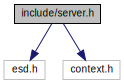
\includegraphics[width=289pt]{d7/d55/server_8h__incl}
\end{center}
\end{figure}
\subsection*{Data Structures}
\begin{DoxyCompactItemize}
\item 
struct \hyperlink{structess__server}{ess\+\_\+server}
\end{DoxyCompactItemize}
\subsection*{Typedefs}
\begin{DoxyCompactItemize}
\item 
typedef enum \hyperlink{server_8h_a54c8d632bfdd95ec349ac2224d7c20df}{ess\+\_\+server\+\_\+status} \hyperlink{server_8h_a66019638fd44eba9d951ec93754c7b8d}{ess\+\_\+server\+\_\+status\+\_\+t}
\item 
typedef struct \hyperlink{structess__server}{ess\+\_\+server} \hyperlink{server_8h_a5265872badf25a007b69f01f94dc60ac}{ess\+\_\+server\+\_\+t}
\end{DoxyCompactItemize}
\subsection*{Enumerations}
\begin{DoxyCompactItemize}
\item 
enum \hyperlink{server_8h_a54c8d632bfdd95ec349ac2224d7c20df}{ess\+\_\+server\+\_\+status} \{ \hyperlink{server_8h_a54c8d632bfdd95ec349ac2224d7c20dfa3e2638ac7c3a94a7d315c36d12aaa107}{E\+S\+S\+\_\+\+S\+E\+R\+V\+E\+R\+\_\+\+S\+T\+A\+T\+U\+S\+\_\+\+S\+T\+OP}, 
\hyperlink{server_8h_a54c8d632bfdd95ec349ac2224d7c20dfa959833bb9f5235bf3c3cdbd217cc0e92}{E\+S\+S\+\_\+\+S\+E\+R\+V\+E\+R\+\_\+\+S\+T\+A\+T\+U\+S\+\_\+\+R\+UN}, 
\hyperlink{server_8h_a54c8d632bfdd95ec349ac2224d7c20dfab58f12c8c17ad2796644350c67a758e6}{E\+S\+S\+\_\+\+S\+E\+R\+V\+E\+R\+\_\+\+S\+T\+A\+T\+U\+S\+\_\+\+S\+T\+A\+N\+D\+BY}, 
\hyperlink{server_8h_a54c8d632bfdd95ec349ac2224d7c20dfa847e6edaa226e5f5fe811a48edb4eeec}{E\+S\+S\+\_\+\+S\+E\+R\+V\+E\+R\+\_\+\+S\+T\+A\+T\+U\+S\+\_\+\+E\+R\+R\+OR}
 \}
\end{DoxyCompactItemize}
\subsection*{Functions}
\begin{DoxyCompactItemize}
\item 
int \hyperlink{server_8h_adc1421ff87cbca2924b87c97bd910ce8}{ess\+\_\+server\+\_\+start} (\hyperlink{server_8h_a5265872badf25a007b69f01f94dc60ac}{ess\+\_\+server\+\_\+t} $\ast$server, const char $\ast$backend\+\_\+name)
\item 
int \hyperlink{server_8h_a7583ec52df3b0560374de87ac987cf09}{ess\+\_\+server\+\_\+stop} (\hyperlink{server_8h_a5265872badf25a007b69f01f94dc60ac}{ess\+\_\+server\+\_\+t} $\ast$server)
\item 
int \hyperlink{server_8h_a74f45549f9048accb7ca06f859298047}{ess\+\_\+restart\+\_\+server} (\hyperlink{server_8h_a5265872badf25a007b69f01f94dc60ac}{ess\+\_\+server\+\_\+t} $\ast$server)
\item 
int \hyperlink{server_8h_a3f4280a20daa813c9309ab51dd32a696}{ess\+\_\+standby\+\_\+server} (\hyperlink{server_8h_a5265872badf25a007b69f01f94dc60ac}{ess\+\_\+server\+\_\+t} $\ast$server)
\item 
int \hyperlink{server_8h_ab0d6ed32ccf3c4601aef38dc6b27b1a1}{ess\+\_\+resume\+\_\+server} (\hyperlink{server_8h_a5265872badf25a007b69f01f94dc60ac}{ess\+\_\+server\+\_\+t} $\ast$server)
\item 
int \hyperlink{server_8h_a6f27a2e3ea0edc392d67de2129fc8a0d}{ess\+\_\+open\+\_\+listen\+\_\+socket} (\hyperlink{server_8h_a5265872badf25a007b69f01f94dc60ac}{ess\+\_\+server\+\_\+t} $\ast$server)
\item 
void \hyperlink{server_8h_ad9d41ce8b8cb5f8d4964fbcf23d3d00e}{ess\+\_\+set\+\_\+audio\+\_\+buffer} (\hyperlink{server_8h_a5265872badf25a007b69f01f94dc60ac}{ess\+\_\+server\+\_\+t} $\ast$server)
\end{DoxyCompactItemize}


\subsection{Typedef Documentation}
\mbox{\Hypertarget{server_8h_a66019638fd44eba9d951ec93754c7b8d}\label{server_8h_a66019638fd44eba9d951ec93754c7b8d}} 
\index{server.\+h@{server.\+h}!ess\+\_\+server\+\_\+status\+\_\+t@{ess\+\_\+server\+\_\+status\+\_\+t}}
\index{ess\+\_\+server\+\_\+status\+\_\+t@{ess\+\_\+server\+\_\+status\+\_\+t}!server.\+h@{server.\+h}}
\subsubsection{\texorpdfstring{ess\+\_\+server\+\_\+status\+\_\+t}{ess\_server\_status\_t}}
{\footnotesize\ttfamily typedef enum \hyperlink{server_8h_a54c8d632bfdd95ec349ac2224d7c20df}{ess\+\_\+server\+\_\+status} \hyperlink{server_8h_a66019638fd44eba9d951ec93754c7b8d}{ess\+\_\+server\+\_\+status\+\_\+t}}

\mbox{\Hypertarget{server_8h_a5265872badf25a007b69f01f94dc60ac}\label{server_8h_a5265872badf25a007b69f01f94dc60ac}} 
\index{server.\+h@{server.\+h}!ess\+\_\+server\+\_\+t@{ess\+\_\+server\+\_\+t}}
\index{ess\+\_\+server\+\_\+t@{ess\+\_\+server\+\_\+t}!server.\+h@{server.\+h}}
\subsubsection{\texorpdfstring{ess\+\_\+server\+\_\+t}{ess\_server\_t}}
{\footnotesize\ttfamily typedef struct \hyperlink{structess__server}{ess\+\_\+server}  \hyperlink{server_8h_a5265872badf25a007b69f01f94dc60ac}{ess\+\_\+server\+\_\+t}}



\subsection{Enumeration Type Documentation}
\mbox{\Hypertarget{server_8h_a54c8d632bfdd95ec349ac2224d7c20df}\label{server_8h_a54c8d632bfdd95ec349ac2224d7c20df}} 
\index{server.\+h@{server.\+h}!ess\+\_\+server\+\_\+status@{ess\+\_\+server\+\_\+status}}
\index{ess\+\_\+server\+\_\+status@{ess\+\_\+server\+\_\+status}!server.\+h@{server.\+h}}
\subsubsection{\texorpdfstring{ess\+\_\+server\+\_\+status}{ess\_server\_status}}
{\footnotesize\ttfamily enum \hyperlink{server_8h_a54c8d632bfdd95ec349ac2224d7c20df}{ess\+\_\+server\+\_\+status}}

\begin{DoxyEnumFields}{Enumerator}
\raisebox{\heightof{T}}[0pt][0pt]{\index{E\+S\+S\+\_\+\+S\+E\+R\+V\+E\+R\+\_\+\+S\+T\+A\+T\+U\+S\+\_\+\+S\+T\+OP@{E\+S\+S\+\_\+\+S\+E\+R\+V\+E\+R\+\_\+\+S\+T\+A\+T\+U\+S\+\_\+\+S\+T\+OP}!server.\+h@{server.\+h}}\index{server.\+h@{server.\+h}!E\+S\+S\+\_\+\+S\+E\+R\+V\+E\+R\+\_\+\+S\+T\+A\+T\+U\+S\+\_\+\+S\+T\+OP@{E\+S\+S\+\_\+\+S\+E\+R\+V\+E\+R\+\_\+\+S\+T\+A\+T\+U\+S\+\_\+\+S\+T\+OP}}}\mbox{\Hypertarget{server_8h_a54c8d632bfdd95ec349ac2224d7c20dfa3e2638ac7c3a94a7d315c36d12aaa107}\label{server_8h_a54c8d632bfdd95ec349ac2224d7c20dfa3e2638ac7c3a94a7d315c36d12aaa107}} 
E\+S\+S\+\_\+\+S\+E\+R\+V\+E\+R\+\_\+\+S\+T\+A\+T\+U\+S\+\_\+\+S\+T\+OP&\\
\hline

\raisebox{\heightof{T}}[0pt][0pt]{\index{E\+S\+S\+\_\+\+S\+E\+R\+V\+E\+R\+\_\+\+S\+T\+A\+T\+U\+S\+\_\+\+R\+UN@{E\+S\+S\+\_\+\+S\+E\+R\+V\+E\+R\+\_\+\+S\+T\+A\+T\+U\+S\+\_\+\+R\+UN}!server.\+h@{server.\+h}}\index{server.\+h@{server.\+h}!E\+S\+S\+\_\+\+S\+E\+R\+V\+E\+R\+\_\+\+S\+T\+A\+T\+U\+S\+\_\+\+R\+UN@{E\+S\+S\+\_\+\+S\+E\+R\+V\+E\+R\+\_\+\+S\+T\+A\+T\+U\+S\+\_\+\+R\+UN}}}\mbox{\Hypertarget{server_8h_a54c8d632bfdd95ec349ac2224d7c20dfa959833bb9f5235bf3c3cdbd217cc0e92}\label{server_8h_a54c8d632bfdd95ec349ac2224d7c20dfa959833bb9f5235bf3c3cdbd217cc0e92}} 
E\+S\+S\+\_\+\+S\+E\+R\+V\+E\+R\+\_\+\+S\+T\+A\+T\+U\+S\+\_\+\+R\+UN&\\
\hline

\raisebox{\heightof{T}}[0pt][0pt]{\index{E\+S\+S\+\_\+\+S\+E\+R\+V\+E\+R\+\_\+\+S\+T\+A\+T\+U\+S\+\_\+\+S\+T\+A\+N\+D\+BY@{E\+S\+S\+\_\+\+S\+E\+R\+V\+E\+R\+\_\+\+S\+T\+A\+T\+U\+S\+\_\+\+S\+T\+A\+N\+D\+BY}!server.\+h@{server.\+h}}\index{server.\+h@{server.\+h}!E\+S\+S\+\_\+\+S\+E\+R\+V\+E\+R\+\_\+\+S\+T\+A\+T\+U\+S\+\_\+\+S\+T\+A\+N\+D\+BY@{E\+S\+S\+\_\+\+S\+E\+R\+V\+E\+R\+\_\+\+S\+T\+A\+T\+U\+S\+\_\+\+S\+T\+A\+N\+D\+BY}}}\mbox{\Hypertarget{server_8h_a54c8d632bfdd95ec349ac2224d7c20dfab58f12c8c17ad2796644350c67a758e6}\label{server_8h_a54c8d632bfdd95ec349ac2224d7c20dfab58f12c8c17ad2796644350c67a758e6}} 
E\+S\+S\+\_\+\+S\+E\+R\+V\+E\+R\+\_\+\+S\+T\+A\+T\+U\+S\+\_\+\+S\+T\+A\+N\+D\+BY&\\
\hline

\raisebox{\heightof{T}}[0pt][0pt]{\index{E\+S\+S\+\_\+\+S\+E\+R\+V\+E\+R\+\_\+\+S\+T\+A\+T\+U\+S\+\_\+\+E\+R\+R\+OR@{E\+S\+S\+\_\+\+S\+E\+R\+V\+E\+R\+\_\+\+S\+T\+A\+T\+U\+S\+\_\+\+E\+R\+R\+OR}!server.\+h@{server.\+h}}\index{server.\+h@{server.\+h}!E\+S\+S\+\_\+\+S\+E\+R\+V\+E\+R\+\_\+\+S\+T\+A\+T\+U\+S\+\_\+\+E\+R\+R\+OR@{E\+S\+S\+\_\+\+S\+E\+R\+V\+E\+R\+\_\+\+S\+T\+A\+T\+U\+S\+\_\+\+E\+R\+R\+OR}}}\mbox{\Hypertarget{server_8h_a54c8d632bfdd95ec349ac2224d7c20dfa847e6edaa226e5f5fe811a48edb4eeec}\label{server_8h_a54c8d632bfdd95ec349ac2224d7c20dfa847e6edaa226e5f5fe811a48edb4eeec}} 
E\+S\+S\+\_\+\+S\+E\+R\+V\+E\+R\+\_\+\+S\+T\+A\+T\+U\+S\+\_\+\+E\+R\+R\+OR&\\
\hline

\end{DoxyEnumFields}


Definition at line 12 of file server.\+h.


\begin{DoxyCode}
12                                \{
13   \hyperlink{server_8h_a54c8d632bfdd95ec349ac2224d7c20dfa3e2638ac7c3a94a7d315c36d12aaa107}{ESS\_SERVER\_STATUS\_STOP},
14   \hyperlink{server_8h_a54c8d632bfdd95ec349ac2224d7c20dfa959833bb9f5235bf3c3cdbd217cc0e92}{ESS\_SERVER\_STATUS\_RUN},
15   \hyperlink{server_8h_a54c8d632bfdd95ec349ac2224d7c20dfab58f12c8c17ad2796644350c67a758e6}{ESS\_SERVER\_STATUS\_STANDBY},
16   \hyperlink{server_8h_a54c8d632bfdd95ec349ac2224d7c20dfa847e6edaa226e5f5fe811a48edb4eeec}{ESS\_SERVER\_STATUS\_ERROR}
17 \}\hyperlink{server_8h_a66019638fd44eba9d951ec93754c7b8d}{ess\_server\_status\_t};
\end{DoxyCode}


\subsection{Function Documentation}
\mbox{\Hypertarget{server_8h_a6f27a2e3ea0edc392d67de2129fc8a0d}\label{server_8h_a6f27a2e3ea0edc392d67de2129fc8a0d}} 
\index{server.\+h@{server.\+h}!ess\+\_\+open\+\_\+listen\+\_\+socket@{ess\+\_\+open\+\_\+listen\+\_\+socket}}
\index{ess\+\_\+open\+\_\+listen\+\_\+socket@{ess\+\_\+open\+\_\+listen\+\_\+socket}!server.\+h@{server.\+h}}
\subsubsection{\texorpdfstring{ess\+\_\+open\+\_\+listen\+\_\+socket()}{ess\_open\_listen\_socket()}}
{\footnotesize\ttfamily int ess\+\_\+open\+\_\+listen\+\_\+socket (\begin{DoxyParamCaption}\item[{\hyperlink{server_8h_a5265872badf25a007b69f01f94dc60ac}{ess\+\_\+server\+\_\+t} $\ast$}]{server }\end{DoxyParamCaption})}

\mbox{\Hypertarget{server_8h_a74f45549f9048accb7ca06f859298047}\label{server_8h_a74f45549f9048accb7ca06f859298047}} 
\index{server.\+h@{server.\+h}!ess\+\_\+restart\+\_\+server@{ess\+\_\+restart\+\_\+server}}
\index{ess\+\_\+restart\+\_\+server@{ess\+\_\+restart\+\_\+server}!server.\+h@{server.\+h}}
\subsubsection{\texorpdfstring{ess\+\_\+restart\+\_\+server()}{ess\_restart\_server()}}
{\footnotesize\ttfamily int ess\+\_\+restart\+\_\+server (\begin{DoxyParamCaption}\item[{\hyperlink{server_8h_a5265872badf25a007b69f01f94dc60ac}{ess\+\_\+server\+\_\+t} $\ast$}]{server }\end{DoxyParamCaption})}

\mbox{\Hypertarget{server_8h_ab0d6ed32ccf3c4601aef38dc6b27b1a1}\label{server_8h_ab0d6ed32ccf3c4601aef38dc6b27b1a1}} 
\index{server.\+h@{server.\+h}!ess\+\_\+resume\+\_\+server@{ess\+\_\+resume\+\_\+server}}
\index{ess\+\_\+resume\+\_\+server@{ess\+\_\+resume\+\_\+server}!server.\+h@{server.\+h}}
\subsubsection{\texorpdfstring{ess\+\_\+resume\+\_\+server()}{ess\_resume\_server()}}
{\footnotesize\ttfamily int ess\+\_\+resume\+\_\+server (\begin{DoxyParamCaption}\item[{\hyperlink{server_8h_a5265872badf25a007b69f01f94dc60ac}{ess\+\_\+server\+\_\+t} $\ast$}]{server }\end{DoxyParamCaption})}

\mbox{\Hypertarget{server_8h_adc1421ff87cbca2924b87c97bd910ce8}\label{server_8h_adc1421ff87cbca2924b87c97bd910ce8}} 
\index{server.\+h@{server.\+h}!ess\+\_\+server\+\_\+start@{ess\+\_\+server\+\_\+start}}
\index{ess\+\_\+server\+\_\+start@{ess\+\_\+server\+\_\+start}!server.\+h@{server.\+h}}
\subsubsection{\texorpdfstring{ess\+\_\+server\+\_\+start()}{ess\_server\_start()}}
{\footnotesize\ttfamily int ess\+\_\+server\+\_\+start (\begin{DoxyParamCaption}\item[{\hyperlink{server_8h_a5265872badf25a007b69f01f94dc60ac}{ess\+\_\+server\+\_\+t} $\ast$}]{server,  }\item[{const char $\ast$}]{backend\+\_\+name }\end{DoxyParamCaption})}

\mbox{\Hypertarget{server_8h_a7583ec52df3b0560374de87ac987cf09}\label{server_8h_a7583ec52df3b0560374de87ac987cf09}} 
\index{server.\+h@{server.\+h}!ess\+\_\+server\+\_\+stop@{ess\+\_\+server\+\_\+stop}}
\index{ess\+\_\+server\+\_\+stop@{ess\+\_\+server\+\_\+stop}!server.\+h@{server.\+h}}
\subsubsection{\texorpdfstring{ess\+\_\+server\+\_\+stop()}{ess\_server\_stop()}}
{\footnotesize\ttfamily int ess\+\_\+server\+\_\+stop (\begin{DoxyParamCaption}\item[{\hyperlink{server_8h_a5265872badf25a007b69f01f94dc60ac}{ess\+\_\+server\+\_\+t} $\ast$}]{server }\end{DoxyParamCaption})}

\mbox{\Hypertarget{server_8h_ad9d41ce8b8cb5f8d4964fbcf23d3d00e}\label{server_8h_ad9d41ce8b8cb5f8d4964fbcf23d3d00e}} 
\index{server.\+h@{server.\+h}!ess\+\_\+set\+\_\+audio\+\_\+buffer@{ess\+\_\+set\+\_\+audio\+\_\+buffer}}
\index{ess\+\_\+set\+\_\+audio\+\_\+buffer@{ess\+\_\+set\+\_\+audio\+\_\+buffer}!server.\+h@{server.\+h}}
\subsubsection{\texorpdfstring{ess\+\_\+set\+\_\+audio\+\_\+buffer()}{ess\_set\_audio\_buffer()}}
{\footnotesize\ttfamily void ess\+\_\+set\+\_\+audio\+\_\+buffer (\begin{DoxyParamCaption}\item[{\hyperlink{server_8h_a5265872badf25a007b69f01f94dc60ac}{ess\+\_\+server\+\_\+t} $\ast$}]{server }\end{DoxyParamCaption})}

\mbox{\Hypertarget{server_8h_a3f4280a20daa813c9309ab51dd32a696}\label{server_8h_a3f4280a20daa813c9309ab51dd32a696}} 
\index{server.\+h@{server.\+h}!ess\+\_\+standby\+\_\+server@{ess\+\_\+standby\+\_\+server}}
\index{ess\+\_\+standby\+\_\+server@{ess\+\_\+standby\+\_\+server}!server.\+h@{server.\+h}}
\subsubsection{\texorpdfstring{ess\+\_\+standby\+\_\+server()}{ess\_standby\_server()}}
{\footnotesize\ttfamily int ess\+\_\+standby\+\_\+server (\begin{DoxyParamCaption}\item[{\hyperlink{server_8h_a5265872badf25a007b69f01f94dc60ac}{ess\+\_\+server\+\_\+t} $\ast$}]{server }\end{DoxyParamCaption})}


\input{d9/dd6/_r_e_a_d_m_e_8md}
\hypertarget{ess__backend_8c}{}\section{src/ess\+\_\+backend.c File Reference}
\label{ess__backend_8c}\index{src/ess\+\_\+backend.\+c@{src/ess\+\_\+backend.\+c}}
{\ttfamily \#include \char`\"{}ess\+\_\+backend.\+h\char`\"{}}\newline
{\ttfamily \#include \char`\"{}ess\+\_\+context.\+h\char`\"{}}\newline
{\ttfamily \#include $<$string.\+h$>$}\newline
{\ttfamily \#include $<$stdlib.\+h$>$}\newline
{\ttfamily \#include $<$stdio.\+h$>$}\newline
{\ttfamily \#include $<$esp\+\_\+log.\+h$>$}\newline
{\ttfamily \#include \char`\"{}ess\+\_\+platform.\+h\char`\"{}}\newline
Include dependency graph for ess\+\_\+backend.\+c\+:
\nopagebreak
\begin{figure}[H]
\begin{center}
\leavevmode
\includegraphics[width=350pt]{db/dcf/ess__backend_8c__incl}
\end{center}
\end{figure}
\subsection*{Macros}
\begin{DoxyCompactItemize}
\item 
\#define \hyperlink{ess__backend_8c_a7ce0df38eb467e59f209470c8f5ac4e6}{L\+O\+G\+\_\+\+T\+AG}~\char`\"{}EssB\char`\"{}
\end{DoxyCompactItemize}
\subsection*{Functions}
\begin{DoxyCompactItemize}
\item 
\hyperlink{ess__backend_8h_ab1487f8c501b38b66796d0fbecb7ed7b}{ess\+\_\+backend\+\_\+facktory\+\_\+t} $\ast$ \hyperlink{ess__backend_8c_a76cca5b79ff4c68316ec3284b78d6436}{ess\+\_\+backend\+\_\+null\+\_\+get\+Factory} ()
\item 
int \hyperlink{ess__backend_8c_a6ba1bf553b596dd14d47748bec40bc9c}{ess\+\_\+backend\+\_\+get\+\_\+size} ()
\begin{DoxyCompactList}\small\item\em get the size of backends \end{DoxyCompactList}\item 
\hyperlink{ess__platform__esp32_8h_ab165b21292abd511e9838af61ab3d331}{ess\+\_\+backends\+\_\+entry\+\_\+t} $\ast$ \hyperlink{ess__backend_8c_a7adfc70995197e0701d33528946f104f}{ess\+\_\+backend\+\_\+get\+\_\+list} (unsigned int $\ast$size)
\item 
\hyperlink{ess__backend_8h_ab1487f8c501b38b66796d0fbecb7ed7b}{ess\+\_\+backend\+\_\+facktory\+\_\+t} $\ast$ \hyperlink{ess__backend_8c_a05e69e3798aee93680d0a024d444212d}{ess\+\_\+backend\+\_\+get\+\_\+by\+\_\+index} (unsigned int index)
\begin{DoxyCompactList}\small\item\em get ess\+\_\+error\+\_\+t entry \end{DoxyCompactList}\item 
\hyperlink{ess__backend_8h_ab1487f8c501b38b66796d0fbecb7ed7b}{ess\+\_\+backend\+\_\+facktory\+\_\+t} $\ast$ \hyperlink{ess__backend_8c_a37052d2bd2290bab5b09bae97dc72719}{ess\+\_\+backend\+\_\+get\+\_\+by\+\_\+name} (const char $\ast$name)
\begin{DoxyCompactList}\small\item\em get ess\+\_\+error\+\_\+t entry \end{DoxyCompactList}\item 
\hyperlink{ess__error_8h_a08ab97fcf6745dee67de912e41bd3236}{ess\+\_\+error\+\_\+t} \hyperlink{ess__backend_8c_ae71b9ae1d68437b482da322b848eafb8}{ess\+\_\+backend\+\_\+probe\+\_\+ex} (const char $\ast$name, \hyperlink{ess__format_8h_a9aa23f58a25b9e8360c1400e0cadfd80}{ess\+\_\+format\+\_\+t} format, \hyperlink{ess__backend_8h_ab1487f8c501b38b66796d0fbecb7ed7b}{ess\+\_\+backend\+\_\+facktory\+\_\+t} $\ast$backend)
\begin{DoxyCompactList}\small\item\em checked the backend with the specified name and returns it if successful. \end{DoxyCompactList}\item 
\hyperlink{ess__error_8h_a08ab97fcf6745dee67de912e41bd3236}{ess\+\_\+error\+\_\+t} \hyperlink{ess__backend_8c_af8adb16ee5aa757492d0cd9b59ed47e7}{ess\+\_\+backend\+\_\+probe} (const \hyperlink{ess__format_8h_a9aa23f58a25b9e8360c1400e0cadfd80}{ess\+\_\+format\+\_\+t} format, \hyperlink{ess__backend_8h_ab1487f8c501b38b66796d0fbecb7ed7b}{ess\+\_\+backend\+\_\+facktory\+\_\+t} $\ast$backend)
\begin{DoxyCompactList}\small\item\em checked the backend \end{DoxyCompactList}\item 
\hyperlink{ess__error_8h_a08ab97fcf6745dee67de912e41bd3236}{ess\+\_\+error\+\_\+t} \hyperlink{ess__backend_8c_a211b7ae8e04be404aa5d883a0e55e81b}{ess\+\_\+backend\+\_\+set\+\_\+sample\+\_\+format} (\hyperlink{ess__backend_8h_ab1487f8c501b38b66796d0fbecb7ed7b}{ess\+\_\+backend\+\_\+facktory\+\_\+t} $\ast$backend, \hyperlink{ess__format_8h_a9aa23f58a25b9e8360c1400e0cadfd80}{ess\+\_\+format\+\_\+t} forma)
\begin{DoxyCompactList}\small\item\em set sample format \end{DoxyCompactList}\item 
void $\ast$ \hyperlink{ess__backend_8c_a5adbfcb9ef73a620c893f59771c3f5e9}{ess\+\_\+backend\+\_\+get\+\_\+user\+\_\+daten} (\hyperlink{ess__backend_8h_ab1487f8c501b38b66796d0fbecb7ed7b}{ess\+\_\+backend\+\_\+facktory\+\_\+t} $\ast$backend)
\begin{DoxyCompactList}\small\item\em get user daten from backend (internal user) \end{DoxyCompactList}\item 
\hyperlink{ess__error_8h_a08ab97fcf6745dee67de912e41bd3236}{ess\+\_\+error\+\_\+t} \hyperlink{ess__backend_8c_a9f84124bcf973ff2a92b2b8ce6798e40}{ess\+\_\+backend\+\_\+set\+\_\+user\+\_\+daten} (\hyperlink{ess__backend_8h_ab1487f8c501b38b66796d0fbecb7ed7b}{ess\+\_\+backend\+\_\+facktory\+\_\+t} $\ast$backend, void $\ast$data)
\begin{DoxyCompactList}\small\item\em set user daten from backend (internal user) \end{DoxyCompactList}\end{DoxyCompactItemize}


\subsection{Macro Definition Documentation}
\mbox{\Hypertarget{ess__backend_8c_a7ce0df38eb467e59f209470c8f5ac4e6}\label{ess__backend_8c_a7ce0df38eb467e59f209470c8f5ac4e6}} 
\index{ess\+\_\+backend.\+c@{ess\+\_\+backend.\+c}!L\+O\+G\+\_\+\+T\+AG@{L\+O\+G\+\_\+\+T\+AG}}
\index{L\+O\+G\+\_\+\+T\+AG@{L\+O\+G\+\_\+\+T\+AG}!ess\+\_\+backend.\+c@{ess\+\_\+backend.\+c}}
\subsubsection{\texorpdfstring{L\+O\+G\+\_\+\+T\+AG}{LOG\_TAG}}
{\footnotesize\ttfamily \#define L\+O\+G\+\_\+\+T\+AG~\char`\"{}EssB\char`\"{}}



Definition at line 36 of file ess\+\_\+backend.\+c.



\subsection{Function Documentation}
\mbox{\Hypertarget{ess__backend_8c_a05e69e3798aee93680d0a024d444212d}\label{ess__backend_8c_a05e69e3798aee93680d0a024d444212d}} 
\index{ess\+\_\+backend.\+c@{ess\+\_\+backend.\+c}!ess\+\_\+backend\+\_\+get\+\_\+by\+\_\+index@{ess\+\_\+backend\+\_\+get\+\_\+by\+\_\+index}}
\index{ess\+\_\+backend\+\_\+get\+\_\+by\+\_\+index@{ess\+\_\+backend\+\_\+get\+\_\+by\+\_\+index}!ess\+\_\+backend.\+c@{ess\+\_\+backend.\+c}}
\subsubsection{\texorpdfstring{ess\+\_\+backend\+\_\+get\+\_\+by\+\_\+index()}{ess\_backend\_get\_by\_index()}}
{\footnotesize\ttfamily \hyperlink{ess__backend_8h_ab1487f8c501b38b66796d0fbecb7ed7b}{ess\+\_\+backend\+\_\+facktory\+\_\+t}$\ast$ ess\+\_\+backend\+\_\+get\+\_\+by\+\_\+index (\begin{DoxyParamCaption}\item[{unsigned int}]{index }\end{DoxyParamCaption})}



get ess\+\_\+error\+\_\+t entry 


\begin{DoxyParams}[1]{Parameters}
\mbox{\tt in}  & {\em number} & of the entry \\
\hline
\end{DoxyParams}
\begin{DoxyReturn}{Returns}
the backend 
\end{DoxyReturn}

\begin{DoxyRetVals}{Return values}
{\em N\+U\+LL} & no backends \\
\hline
\end{DoxyRetVals}


Definition at line 57 of file ess\+\_\+backend.\+c.


\begin{DoxyCode}
57                                                                       \{
58   \textcolor{keywordflow}{if}(index > \hyperlink{ess__backend_8c_a6ba1bf553b596dd14d47748bec40bc9c}{ess\_backend\_get\_size}() ) \textcolor{keywordflow}{return} 0;
59   \textcolor{keywordflow}{return} \hyperlink{ess__platform__esp32_8h_a0aae1a44ffbe4df0c0b4d13810ec8e22}{backends\_list}[index].\hyperlink{structess__backends__entry_a86f760dbdba11d491bc8209327d7e514}{getFactory}();
60 \}
\end{DoxyCode}
Here is the call graph for this function\+:
\nopagebreak
\begin{figure}[H]
\begin{center}
\leavevmode
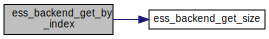
\includegraphics[width=341pt]{d8/d50/ess__backend_8c_a05e69e3798aee93680d0a024d444212d_cgraph}
\end{center}
\end{figure}
Here is the caller graph for this function\+:
\nopagebreak
\begin{figure}[H]
\begin{center}
\leavevmode
\includegraphics[width=284pt]{d8/d50/ess__backend_8c_a05e69e3798aee93680d0a024d444212d_icgraph}
\end{center}
\end{figure}
\mbox{\Hypertarget{ess__backend_8c_a37052d2bd2290bab5b09bae97dc72719}\label{ess__backend_8c_a37052d2bd2290bab5b09bae97dc72719}} 
\index{ess\+\_\+backend.\+c@{ess\+\_\+backend.\+c}!ess\+\_\+backend\+\_\+get\+\_\+by\+\_\+name@{ess\+\_\+backend\+\_\+get\+\_\+by\+\_\+name}}
\index{ess\+\_\+backend\+\_\+get\+\_\+by\+\_\+name@{ess\+\_\+backend\+\_\+get\+\_\+by\+\_\+name}!ess\+\_\+backend.\+c@{ess\+\_\+backend.\+c}}
\subsubsection{\texorpdfstring{ess\+\_\+backend\+\_\+get\+\_\+by\+\_\+name()}{ess\_backend\_get\_by\_name()}}
{\footnotesize\ttfamily \hyperlink{ess__backend_8h_ab1487f8c501b38b66796d0fbecb7ed7b}{ess\+\_\+backend\+\_\+facktory\+\_\+t}$\ast$ ess\+\_\+backend\+\_\+get\+\_\+by\+\_\+name (\begin{DoxyParamCaption}\item[{const char $\ast$}]{name }\end{DoxyParamCaption})}



get ess\+\_\+error\+\_\+t entry 


\begin{DoxyParams}[1]{Parameters}
\mbox{\tt in}  & {\em name} & of the backend \\
\hline
\end{DoxyParams}
\begin{DoxyReturn}{Returns}
the backend 
\end{DoxyReturn}

\begin{DoxyRetVals}{Return values}
{\em N\+U\+LL} & no backends \\
\hline
\end{DoxyRetVals}


Definition at line 63 of file ess\+\_\+backend.\+c.


\begin{DoxyCode}
63                                                                    \{
64   \hyperlink{structess__backend}{ess\_backend\_facktory\_t}* factory = 0;
65 
66   \textcolor{keywordflow}{for}(\textcolor{keywordtype}{unsigned} \textcolor{keywordtype}{int} i = 0; i < \hyperlink{ess__backend_8c_a6ba1bf553b596dd14d47748bec40bc9c}{ess\_backend\_get\_size}(); i++ ) \{
67     \textcolor{keywordflow}{if}(strcmp(\hyperlink{ess__platform__esp32_8h_a0aae1a44ffbe4df0c0b4d13810ec8e22}{backends\_list}[i].name, name)) \{
68       factory = \hyperlink{ess__platform__esp32_8h_a0aae1a44ffbe4df0c0b4d13810ec8e22}{backends\_list}[i].\hyperlink{structess__backends__entry_a86f760dbdba11d491bc8209327d7e514}{getFactory}();
69       \textcolor{keywordflow}{break};
70     \}
71   \}
72   \textcolor{keywordflow}{return} factory;
73 \}
\end{DoxyCode}
Here is the call graph for this function\+:
\nopagebreak
\begin{figure}[H]
\begin{center}
\leavevmode
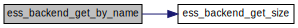
\includegraphics[width=350pt]{d8/d50/ess__backend_8c_a37052d2bd2290bab5b09bae97dc72719_cgraph}
\end{center}
\end{figure}
Here is the caller graph for this function\+:
\nopagebreak
\begin{figure}[H]
\begin{center}
\leavevmode
\includegraphics[width=350pt]{d8/d50/ess__backend_8c_a37052d2bd2290bab5b09bae97dc72719_icgraph}
\end{center}
\end{figure}
\mbox{\Hypertarget{ess__backend_8c_a7adfc70995197e0701d33528946f104f}\label{ess__backend_8c_a7adfc70995197e0701d33528946f104f}} 
\index{ess\+\_\+backend.\+c@{ess\+\_\+backend.\+c}!ess\+\_\+backend\+\_\+get\+\_\+list@{ess\+\_\+backend\+\_\+get\+\_\+list}}
\index{ess\+\_\+backend\+\_\+get\+\_\+list@{ess\+\_\+backend\+\_\+get\+\_\+list}!ess\+\_\+backend.\+c@{ess\+\_\+backend.\+c}}
\subsubsection{\texorpdfstring{ess\+\_\+backend\+\_\+get\+\_\+list()}{ess\_backend\_get\_list()}}
{\footnotesize\ttfamily \hyperlink{ess__platform__esp32_8h_ab165b21292abd511e9838af61ab3d331}{ess\+\_\+backends\+\_\+entry\+\_\+t}$\ast$ ess\+\_\+backend\+\_\+get\+\_\+list (\begin{DoxyParamCaption}\item[{unsigned int $\ast$}]{size }\end{DoxyParamCaption})}



Definition at line 52 of file ess\+\_\+backend.\+c.


\begin{DoxyCode}
52                                                                \{
53   \textcolor{keywordflow}{if}(size != 0) *size = ( \textcolor{keyword}{sizeof}(\hyperlink{ess__platform__esp32_8h_a0aae1a44ffbe4df0c0b4d13810ec8e22}{backends\_list}) / \textcolor{keyword}{sizeof}(
      \hyperlink{structess__backends__entry}{ess\_backends\_entry\_t}) );
54   \textcolor{keywordflow}{return} \hyperlink{ess__platform__esp32_8h_a0aae1a44ffbe4df0c0b4d13810ec8e22}{backends\_list};
55 \}
\end{DoxyCode}
\mbox{\Hypertarget{ess__backend_8c_a6ba1bf553b596dd14d47748bec40bc9c}\label{ess__backend_8c_a6ba1bf553b596dd14d47748bec40bc9c}} 
\index{ess\+\_\+backend.\+c@{ess\+\_\+backend.\+c}!ess\+\_\+backend\+\_\+get\+\_\+size@{ess\+\_\+backend\+\_\+get\+\_\+size}}
\index{ess\+\_\+backend\+\_\+get\+\_\+size@{ess\+\_\+backend\+\_\+get\+\_\+size}!ess\+\_\+backend.\+c@{ess\+\_\+backend.\+c}}
\subsubsection{\texorpdfstring{ess\+\_\+backend\+\_\+get\+\_\+size()}{ess\_backend\_get\_size()}}
{\footnotesize\ttfamily int ess\+\_\+backend\+\_\+get\+\_\+size (\begin{DoxyParamCaption}{ }\end{DoxyParamCaption})}



get the size of backends 

\begin{DoxyReturn}{Returns}
the number of platform backends in the list 
\end{DoxyReturn}


Definition at line 49 of file ess\+\_\+backend.\+c.


\begin{DoxyCode}
49                            \{
50   \textcolor{keywordflow}{return} \textcolor{keyword}{sizeof}(\hyperlink{ess__platform__esp32_8h_a0aae1a44ffbe4df0c0b4d13810ec8e22}{backends\_list}) / \textcolor{keyword}{sizeof}(\hyperlink{structess__backends__entry}{ess\_backends\_entry\_t});
51 \}
\end{DoxyCode}
Here is the caller graph for this function\+:
\nopagebreak
\begin{figure}[H]
\begin{center}
\leavevmode
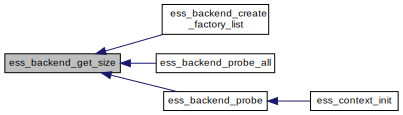
\includegraphics[width=350pt]{d8/d50/ess__backend_8c_a6ba1bf553b596dd14d47748bec40bc9c_icgraph}
\end{center}
\end{figure}
\mbox{\Hypertarget{ess__backend_8c_a5adbfcb9ef73a620c893f59771c3f5e9}\label{ess__backend_8c_a5adbfcb9ef73a620c893f59771c3f5e9}} 
\index{ess\+\_\+backend.\+c@{ess\+\_\+backend.\+c}!ess\+\_\+backend\+\_\+get\+\_\+user\+\_\+daten@{ess\+\_\+backend\+\_\+get\+\_\+user\+\_\+daten}}
\index{ess\+\_\+backend\+\_\+get\+\_\+user\+\_\+daten@{ess\+\_\+backend\+\_\+get\+\_\+user\+\_\+daten}!ess\+\_\+backend.\+c@{ess\+\_\+backend.\+c}}
\subsubsection{\texorpdfstring{ess\+\_\+backend\+\_\+get\+\_\+user\+\_\+daten()}{ess\_backend\_get\_user\_daten()}}
{\footnotesize\ttfamily void$\ast$ ess\+\_\+backend\+\_\+get\+\_\+user\+\_\+daten (\begin{DoxyParamCaption}\item[{\hyperlink{ess__backend_8h_ab1487f8c501b38b66796d0fbecb7ed7b}{ess\+\_\+backend\+\_\+facktory\+\_\+t} $\ast$}]{backend }\end{DoxyParamCaption})}



get user daten from backend (internal user) 


\begin{DoxyParams}[1]{Parameters}
\mbox{\tt in}  & {\em the} & using backend \\
\hline
\end{DoxyParams}
\begin{DoxyReturn}{Returns}
the user daten 
\end{DoxyReturn}


Definition at line 96 of file ess\+\_\+backend.\+c.


\begin{DoxyCode}
96                                                                   \{
97   \textcolor{keywordflow}{if}(backend == 0)  \textcolor{keywordflow}{return} 0;
98   \textcolor{keywordflow}{return}  backend->\hyperlink{structess__backend_a5ad8569143b4728c7b7f91c53661d8b5}{user\_daten};
99 \}
\end{DoxyCode}
\mbox{\Hypertarget{ess__backend_8c_a76cca5b79ff4c68316ec3284b78d6436}\label{ess__backend_8c_a76cca5b79ff4c68316ec3284b78d6436}} 
\index{ess\+\_\+backend.\+c@{ess\+\_\+backend.\+c}!ess\+\_\+backend\+\_\+null\+\_\+get\+Factory@{ess\+\_\+backend\+\_\+null\+\_\+get\+Factory}}
\index{ess\+\_\+backend\+\_\+null\+\_\+get\+Factory@{ess\+\_\+backend\+\_\+null\+\_\+get\+Factory}!ess\+\_\+backend.\+c@{ess\+\_\+backend.\+c}}
\subsubsection{\texorpdfstring{ess\+\_\+backend\+\_\+null\+\_\+get\+Factory()}{ess\_backend\_null\_getFactory()}}
{\footnotesize\ttfamily \hyperlink{ess__backend_8h_ab1487f8c501b38b66796d0fbecb7ed7b}{ess\+\_\+backend\+\_\+facktory\+\_\+t}$\ast$ ess\+\_\+backend\+\_\+null\+\_\+get\+Factory (\begin{DoxyParamCaption}{ }\end{DoxyParamCaption})}



Definition at line 88 of file null\+\_\+backend.\+c.


\begin{DoxyCode}
88                                                       \{
89   \textcolor{keywordflow}{return} &\hyperlink{null__backend_8c_a53217e29e5207ff3a61873b4ed0eac2a}{\_null\_backend\_config};
90 \}
\end{DoxyCode}
\mbox{\Hypertarget{ess__backend_8c_af8adb16ee5aa757492d0cd9b59ed47e7}\label{ess__backend_8c_af8adb16ee5aa757492d0cd9b59ed47e7}} 
\index{ess\+\_\+backend.\+c@{ess\+\_\+backend.\+c}!ess\+\_\+backend\+\_\+probe@{ess\+\_\+backend\+\_\+probe}}
\index{ess\+\_\+backend\+\_\+probe@{ess\+\_\+backend\+\_\+probe}!ess\+\_\+backend.\+c@{ess\+\_\+backend.\+c}}
\subsubsection{\texorpdfstring{ess\+\_\+backend\+\_\+probe()}{ess\_backend\_probe()}}
{\footnotesize\ttfamily \hyperlink{ess__error_8h_a08ab97fcf6745dee67de912e41bd3236}{ess\+\_\+error\+\_\+t} ess\+\_\+backend\+\_\+probe (\begin{DoxyParamCaption}\item[{const \hyperlink{ess__format_8h_a9aa23f58a25b9e8360c1400e0cadfd80}{ess\+\_\+format\+\_\+t}}]{format,  }\item[{\hyperlink{ess__backend_8h_ab1487f8c501b38b66796d0fbecb7ed7b}{ess\+\_\+backend\+\_\+facktory\+\_\+t} $\ast$}]{backend }\end{DoxyParamCaption})}



checked the backend 


\begin{DoxyParams}[1]{Parameters}
\mbox{\tt in}  & {\em format} & the format to probe \\
\hline
\mbox{\tt in}  & {\em backend} & return the working backend. if not null \\
\hline
\end{DoxyParams}

\begin{DoxyRetVals}{Return values}
{\em E\+S\+S\+\_\+\+OK} & if backend support \\
\hline
{\em E\+S\+S\+\_\+\+E\+R\+R\+O\+R\+\_\+\+W\+R\+O\+N\+G\+\_\+\+F\+O\+R\+M\+AT} & \\
\hline
{\em E\+S\+S\+\_\+\+E\+R\+R\+O\+R\+\_\+\+N\+U\+LL} & backend is null \\
\hline
\end{DoxyRetVals}


Definition at line 88 of file ess\+\_\+backend.\+c.


\begin{DoxyCode}
88                                                                                           \{
89   \textcolor{keywordflow}{if}(backend == 0) \textcolor{keywordflow}{return} \hyperlink{ess__error_8h_a3a40ffb47f45a17c8989af8286e7a07fa96978468215ef7117c99232e72d7fb39}{ESS\_ERROR\_NULL};
90   \textcolor{keywordflow}{return} backend->\hyperlink{structess__backend_a7a51d8dd3864c93fb26e193353e0f3bd}{ess\_backend\_probe}(format);
91 \}
\end{DoxyCode}
Here is the caller graph for this function\+:
\nopagebreak
\begin{figure}[H]
\begin{center}
\leavevmode
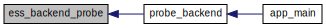
\includegraphics[width=350pt]{d8/d50/ess__backend_8c_af8adb16ee5aa757492d0cd9b59ed47e7_icgraph}
\end{center}
\end{figure}
\mbox{\Hypertarget{ess__backend_8c_ae71b9ae1d68437b482da322b848eafb8}\label{ess__backend_8c_ae71b9ae1d68437b482da322b848eafb8}} 
\index{ess\+\_\+backend.\+c@{ess\+\_\+backend.\+c}!ess\+\_\+backend\+\_\+probe\+\_\+ex@{ess\+\_\+backend\+\_\+probe\+\_\+ex}}
\index{ess\+\_\+backend\+\_\+probe\+\_\+ex@{ess\+\_\+backend\+\_\+probe\+\_\+ex}!ess\+\_\+backend.\+c@{ess\+\_\+backend.\+c}}
\subsubsection{\texorpdfstring{ess\+\_\+backend\+\_\+probe\+\_\+ex()}{ess\_backend\_probe\_ex()}}
{\footnotesize\ttfamily \hyperlink{ess__error_8h_a08ab97fcf6745dee67de912e41bd3236}{ess\+\_\+error\+\_\+t} ess\+\_\+backend\+\_\+probe\+\_\+ex (\begin{DoxyParamCaption}\item[{const char $\ast$}]{name,  }\item[{const \hyperlink{ess__format_8h_a9aa23f58a25b9e8360c1400e0cadfd80}{ess\+\_\+format\+\_\+t}}]{format,  }\item[{\hyperlink{ess__backend_8h_ab1487f8c501b38b66796d0fbecb7ed7b}{ess\+\_\+backend\+\_\+facktory\+\_\+t} $\ast$}]{backend }\end{DoxyParamCaption})}



checked the backend with the specified name and returns it if successful. 


\begin{DoxyParams}[1]{Parameters}
\mbox{\tt in}  & {\em Name} & of the backend \\
\hline
\mbox{\tt in}  & {\em format} & the format to probe \\
\hline
\mbox{\tt out}  & {\em backend} & return the working backend. if not null\\
\hline
\end{DoxyParams}

\begin{DoxyRetVals}{Return values}
{\em E\+S\+S\+\_\+\+OK} & if backend support \\
\hline
{\em E\+S\+S\+\_\+\+E\+R\+R\+O\+R\+\_\+\+W\+R\+O\+N\+G\+\_\+\+F\+O\+R\+M\+AT} & \\
\hline
{\em E\+S\+S\+\_\+\+E\+R\+R\+OR} & \\
\hline
\end{DoxyRetVals}


Definition at line 75 of file ess\+\_\+backend.\+c.


\begin{DoxyCode}
75                                                                                                          \{
76   \textcolor{keywordflow}{for}(\textcolor{keywordtype}{unsigned} \textcolor{keywordtype}{int} i = 0; i < \hyperlink{ess__backend_8c_a6ba1bf553b596dd14d47748bec40bc9c}{ess\_backend\_get\_size}(); i++ ) \{
77     \textcolor{keywordflow}{if}(strcmp(\hyperlink{ess__platform__esp32_8h_a0aae1a44ffbe4df0c0b4d13810ec8e22}{backends\_list}[i].name, name)) \{
78       \textcolor{keywordflow}{if}(\hyperlink{ess__platform__esp32_8h_a0aae1a44ffbe4df0c0b4d13810ec8e22}{backends\_list}[i].getFactory()->ess\_backend\_probe(format) == 
      \hyperlink{ess__error_8h_a3a40ffb47f45a17c8989af8286e7a07fa7a39eb24d172b29cca7678967088d864}{ESS\_OK}) \{
79         \textcolor{keywordflow}{if}(backend) backend = \hyperlink{ess__platform__esp32_8h_a0aae1a44ffbe4df0c0b4d13810ec8e22}{backends\_list}[i].\hyperlink{structess__backends__entry_a86f760dbdba11d491bc8209327d7e514}{getFactory}();
80         \textcolor{keywordflow}{return} \hyperlink{ess__error_8h_a3a40ffb47f45a17c8989af8286e7a07fa7a39eb24d172b29cca7678967088d864}{ESS\_OK};
81       \} \textcolor{keywordflow}{else} \{
82         \textcolor{keywordflow}{return} \hyperlink{ess__error_8h_a3a40ffb47f45a17c8989af8286e7a07fa7ba47a8b8e91f5506ab2efa391919d80}{ESS\_ERROR\_WRONG\_FORMAT};
83       \}
84     \}
85   \}
86   \textcolor{keywordflow}{return} \hyperlink{ess__error_8h_a3a40ffb47f45a17c8989af8286e7a07faa28e2c57627994f0cfa08dd3b4e28b97}{ESS\_ERROR};
87 \}
\end{DoxyCode}
Here is the call graph for this function\+:
\nopagebreak
\begin{figure}[H]
\begin{center}
\leavevmode
\includegraphics[width=350pt]{d8/d50/ess__backend_8c_ae71b9ae1d68437b482da322b848eafb8_cgraph}
\end{center}
\end{figure}
\mbox{\Hypertarget{ess__backend_8c_a211b7ae8e04be404aa5d883a0e55e81b}\label{ess__backend_8c_a211b7ae8e04be404aa5d883a0e55e81b}} 
\index{ess\+\_\+backend.\+c@{ess\+\_\+backend.\+c}!ess\+\_\+backend\+\_\+set\+\_\+sample\+\_\+format@{ess\+\_\+backend\+\_\+set\+\_\+sample\+\_\+format}}
\index{ess\+\_\+backend\+\_\+set\+\_\+sample\+\_\+format@{ess\+\_\+backend\+\_\+set\+\_\+sample\+\_\+format}!ess\+\_\+backend.\+c@{ess\+\_\+backend.\+c}}
\subsubsection{\texorpdfstring{ess\+\_\+backend\+\_\+set\+\_\+sample\+\_\+format()}{ess\_backend\_set\_sample\_format()}}
{\footnotesize\ttfamily \hyperlink{ess__error_8h_a08ab97fcf6745dee67de912e41bd3236}{ess\+\_\+error\+\_\+t} ess\+\_\+backend\+\_\+set\+\_\+sample\+\_\+format (\begin{DoxyParamCaption}\item[{\hyperlink{ess__backend_8h_ab1487f8c501b38b66796d0fbecb7ed7b}{ess\+\_\+backend\+\_\+facktory\+\_\+t} $\ast$}]{backend,  }\item[{const \hyperlink{ess__format_8h_a9aa23f58a25b9e8360c1400e0cadfd80}{ess\+\_\+format\+\_\+t}}]{forma }\end{DoxyParamCaption})}



set sample format 


\begin{DoxyParams}[1]{Parameters}
\mbox{\tt in}  & {\em backend} & the usiing backend \\
\hline
\mbox{\tt in}  & {\em forma} & sample format \\
\hline
\end{DoxyParams}

\begin{DoxyRetVals}{Return values}
{\em E\+S\+S\+\_\+\+OK} & if backend support \\
\hline
{\em E\+S\+S\+\_\+\+E\+R\+R\+O\+R\+\_\+\+W\+R\+O\+N\+G\+\_\+\+F\+O\+R\+M\+AT} & \\
\hline
{\em E\+S\+S\+\_\+\+E\+R\+R\+OR} & \\
\hline
\end{DoxyRetVals}


Definition at line 92 of file ess\+\_\+backend.\+c.


\begin{DoxyCode}
92                                                                                                 \{
93   \textcolor{keywordflow}{if}(backend == 0) \textcolor{keywordflow}{return} \hyperlink{ess__error_8h_a3a40ffb47f45a17c8989af8286e7a07fa96978468215ef7117c99232e72d7fb39}{ESS\_ERROR\_NULL};
94   \textcolor{keywordflow}{return} backend->\hyperlink{structess__backend_ab081e20cac5828678d80e03f5182a155}{ess\_backend\_set\_sample\_format}(forma);
95 \}
\end{DoxyCode}
Here is the caller graph for this function\+:
\nopagebreak
\begin{figure}[H]
\begin{center}
\leavevmode
\includegraphics[width=350pt]{d8/d50/ess__backend_8c_a211b7ae8e04be404aa5d883a0e55e81b_icgraph}
\end{center}
\end{figure}
\mbox{\Hypertarget{ess__backend_8c_a9f84124bcf973ff2a92b2b8ce6798e40}\label{ess__backend_8c_a9f84124bcf973ff2a92b2b8ce6798e40}} 
\index{ess\+\_\+backend.\+c@{ess\+\_\+backend.\+c}!ess\+\_\+backend\+\_\+set\+\_\+user\+\_\+daten@{ess\+\_\+backend\+\_\+set\+\_\+user\+\_\+daten}}
\index{ess\+\_\+backend\+\_\+set\+\_\+user\+\_\+daten@{ess\+\_\+backend\+\_\+set\+\_\+user\+\_\+daten}!ess\+\_\+backend.\+c@{ess\+\_\+backend.\+c}}
\subsubsection{\texorpdfstring{ess\+\_\+backend\+\_\+set\+\_\+user\+\_\+daten()}{ess\_backend\_set\_user\_daten()}}
{\footnotesize\ttfamily \hyperlink{ess__error_8h_a08ab97fcf6745dee67de912e41bd3236}{ess\+\_\+error\+\_\+t} ess\+\_\+backend\+\_\+set\+\_\+user\+\_\+daten (\begin{DoxyParamCaption}\item[{\hyperlink{ess__backend_8h_ab1487f8c501b38b66796d0fbecb7ed7b}{ess\+\_\+backend\+\_\+facktory\+\_\+t} $\ast$}]{backend,  }\item[{void $\ast$}]{data }\end{DoxyParamCaption})}



set user daten from backend (internal user) 


\begin{DoxyParams}[1]{Parameters}
\mbox{\tt in}  & {\em the} & usiing backend \\
\hline
\mbox{\tt in}  & {\em data} & the using data \\
\hline
\end{DoxyParams}

\begin{DoxyRetVals}{Return values}
{\em E\+S\+S\+\_\+\+OK} & \\
\hline
{\em E\+S\+S\+\_\+\+E\+R\+R\+O\+R\+\_\+\+N\+U\+LL} & backend null \\
\hline
\end{DoxyRetVals}


Definition at line 100 of file ess\+\_\+backend.\+c.


\begin{DoxyCode}
100                                                                                     \{
101   \textcolor{keywordflow}{if}(backend == 0)  \textcolor{keywordflow}{return} \hyperlink{ess__error_8h_a3a40ffb47f45a17c8989af8286e7a07fa96978468215ef7117c99232e72d7fb39}{ESS\_ERROR\_NULL};
102   backend->\hyperlink{structess__backend_a5ad8569143b4728c7b7f91c53661d8b5}{user\_daten} = data;
103   \textcolor{keywordflow}{return} \hyperlink{ess__error_8h_a3a40ffb47f45a17c8989af8286e7a07fa7a39eb24d172b29cca7678967088d864}{ESS\_OK};
104 \}
\end{DoxyCode}

\hypertarget{ess__context_8c}{}\section{src/ess\+\_\+context.c File Reference}
\label{ess__context_8c}\index{src/ess\+\_\+context.\+c@{src/ess\+\_\+context.\+c}}
{\ttfamily \#include \char`\"{}ess\+\_\+context.\+h\char`\"{}}\newline
{\ttfamily \#include \char`\"{}ess\+\_\+backend.\+h\char`\"{}}\newline
{\ttfamily \#include $<$string.\+h$>$}\newline
{\ttfamily \#include $<$stdlib.\+h$>$}\newline
{\ttfamily \#include $<$stdio.\+h$>$}\newline
{\ttfamily \#include $<$esp\+\_\+log.\+h$>$}\newline
{\ttfamily \#include \char`\"{}config.\+h\char`\"{}}\newline
Include dependency graph for ess\+\_\+context.\+c\+:\nopagebreak
\begin{figure}[H]
\begin{center}
\leavevmode
\includegraphics[width=350pt]{d9/d9d/ess__context_8c__incl}
\end{center}
\end{figure}
\subsection*{Macros}
\begin{DoxyCompactItemize}
\item 
\#define \hyperlink{ess__context_8c_a7ce0df38eb467e59f209470c8f5ac4e6}{L\+O\+G\+\_\+\+T\+AG}~\char`\"{}EssC\char`\"{}
\end{DoxyCompactItemize}
\subsection*{Functions}
\begin{DoxyCompactItemize}
\item 
\hyperlink{ess__context_8h_acc807999e4f53d1867abf8a0ac682f33}{ess\+\_\+context\+\_\+error\+\_\+t} \hyperlink{ess__context_8c_ac764fbb6b72712d2b755f54c6b240e33}{ess\+\_\+context\+\_\+create} (\hyperlink{ess__context_8h_a8a8fec5766c0b3615f8f12f7948e949b}{ess\+\_\+context\+\_\+t} $\ast$context, const \hyperlink{ess__format_8h_ab03f24cb5d42f4448f713bf1ec178163}{ess\+\_\+format\+\_\+t} format)
\begin{DoxyCompactList}\small\item\em creater the context \end{DoxyCompactList}\item 
\hyperlink{ess__context_8h_acc807999e4f53d1867abf8a0ac682f33}{ess\+\_\+context\+\_\+error\+\_\+t} \hyperlink{ess__context_8c_a40a2211f2793b0346c879b61b35ff63e}{ess\+\_\+context\+\_\+init} (\hyperlink{ess__context_8h_a8a8fec5766c0b3615f8f12f7948e949b}{ess\+\_\+context\+\_\+t} $\ast$context, const char $\ast$name)
\begin{DoxyCompactList}\small\item\em initialisiert the context \end{DoxyCompactList}\item 
\hyperlink{ess__context_8h_acc807999e4f53d1867abf8a0ac682f33}{ess\+\_\+context\+\_\+error\+\_\+t} \hyperlink{ess__context_8c_a26ae0093adaa4a6945fed6cfd31d4ae7}{ess\+\_\+context\+\_\+init\+\_\+ex} (\hyperlink{ess__context_8h_a8a8fec5766c0b3615f8f12f7948e949b}{ess\+\_\+context\+\_\+t} $\ast$context, \hyperlink{ess__backend_8h_ab1487f8c501b38b66796d0fbecb7ed7b}{ess\+\_\+backend\+\_\+facktory\+\_\+t} $\ast$backend)
\begin{DoxyCompactList}\small\item\em initialisiert the context with a user backend \end{DoxyCompactList}\item 
\hyperlink{ess__context_8h_acc807999e4f53d1867abf8a0ac682f33}{ess\+\_\+context\+\_\+error\+\_\+t} \hyperlink{ess__context_8c_a9a12468e0f826cc92385be2df34a38d4}{ess\+\_\+context\+\_\+close} (\hyperlink{ess__context_8h_a8a8fec5766c0b3615f8f12f7948e949b}{ess\+\_\+context\+\_\+t} $\ast$context)
\begin{DoxyCompactList}\small\item\em close the context and close the backend \end{DoxyCompactList}\item 
\hyperlink{ess__context_8h_acc807999e4f53d1867abf8a0ac682f33}{ess\+\_\+context\+\_\+error\+\_\+t} \hyperlink{ess__context_8c_a0a9e96c03cba2bfef2999c0199070d17}{ess\+\_\+context\+\_\+destroy} (\hyperlink{ess__context_8h_a8a8fec5766c0b3615f8f12f7948e949b}{ess\+\_\+context\+\_\+t} $\ast$context)
\begin{DoxyCompactList}\small\item\em destroy and free the context \end{DoxyCompactList}\item 
\hyperlink{ess__context_8h_acc807999e4f53d1867abf8a0ac682f33}{ess\+\_\+context\+\_\+error\+\_\+t} \hyperlink{ess__context_8c_a6b450cd4cfd4fed931f99b05c38e0172}{ess\+\_\+context\+\_\+paused} (\hyperlink{ess__context_8h_a8a8fec5766c0b3615f8f12f7948e949b}{ess\+\_\+context\+\_\+t} $\ast$context)
\begin{DoxyCompactList}\small\item\em set backend to standby \end{DoxyCompactList}\item 
\hyperlink{ess__context_8h_acc807999e4f53d1867abf8a0ac682f33}{ess\+\_\+context\+\_\+error\+\_\+t} \hyperlink{ess__context_8c_ac6041313862e70f48b8441df8136b0ba}{ess\+\_\+context\+\_\+resume} (\hyperlink{ess__context_8h_a8a8fec5766c0b3615f8f12f7948e949b}{ess\+\_\+context\+\_\+t} $\ast$context)
\begin{DoxyCompactList}\small\item\em set backend to run \end{DoxyCompactList}\item 
\hyperlink{ess__context_8h_acc807999e4f53d1867abf8a0ac682f33}{ess\+\_\+context\+\_\+error\+\_\+t} \hyperlink{ess__context_8c_aebeaf3ec64fe0e348557884dfa601944}{ess\+\_\+context\+\_\+set\+\_\+format} (\hyperlink{ess__context_8h_a8a8fec5766c0b3615f8f12f7948e949b}{ess\+\_\+context\+\_\+t} $\ast$context, const \hyperlink{ess__format_8h_ab03f24cb5d42f4448f713bf1ec178163}{ess\+\_\+format\+\_\+t} format)
\begin{DoxyCompactList}\small\item\em set the sample format to backend \end{DoxyCompactList}\item 
unsigned int \hyperlink{ess__context_8c_ae2c6a4e2f8a5128fc1bb05afea5f3c8d}{ess\+\_\+context\+\_\+write} (\hyperlink{ess__context_8h_a8a8fec5766c0b3615f8f12f7948e949b}{ess\+\_\+context\+\_\+t} $\ast$context, void $\ast$buffer, unsigned int buf\+\_\+size)
\begin{DoxyCompactList}\small\item\em write audio data to the backend \end{DoxyCompactList}\item 
\hyperlink{ess__context_8h_acc807999e4f53d1867abf8a0ac682f33}{ess\+\_\+context\+\_\+error\+\_\+t} \hyperlink{ess__context_8c_a8077482da675241fd832152974033994}{ess\+\_\+context\+\_\+write\+\_\+ex} (\hyperlink{ess__context_8h_a8a8fec5766c0b3615f8f12f7948e949b}{ess\+\_\+context\+\_\+t} $\ast$context, void $\ast$buffer, unsigned int buf\+\_\+size, unsigned int $\ast$wrote)
\begin{DoxyCompactList}\small\item\em write audio data to the backend \end{DoxyCompactList}\item 
const char $\ast$ \hyperlink{ess__context_8c_a1038af3d90a5a8a45d4fc35cbd425e5b}{ess\+\_\+context\+\_\+get\+\_\+backend\+\_\+name} (\hyperlink{ess__context_8h_a8a8fec5766c0b3615f8f12f7948e949b}{ess\+\_\+context\+\_\+t} $\ast$context)
\begin{DoxyCompactList}\small\item\em get the usind backend name \end{DoxyCompactList}\item 
const char $\ast$ \hyperlink{ess__context_8c_a139494e2518952f79ec0bc7d788d7612}{ess\+\_\+context\+\_\+get\+\_\+backend\+\_\+info} (\hyperlink{ess__context_8h_a8a8fec5766c0b3615f8f12f7948e949b}{ess\+\_\+context\+\_\+t} $\ast$context)
\begin{DoxyCompactList}\small\item\em get using backend informations \end{DoxyCompactList}\item 
\hyperlink{ess__context_8h_acc807999e4f53d1867abf8a0ac682f33}{ess\+\_\+context\+\_\+error\+\_\+t} \hyperlink{ess__context_8c_ae8c078f30231eae2756ff85825dac90a}{ess\+\_\+context\+\_\+get\+\_\+last\+\_\+error} (\hyperlink{ess__context_8h_a8a8fec5766c0b3615f8f12f7948e949b}{ess\+\_\+context\+\_\+t} $\ast$context)
\begin{DoxyCompactList}\small\item\em get the last error from context \end{DoxyCompactList}\end{DoxyCompactItemize}


\subsection{Macro Definition Documentation}
\mbox{\Hypertarget{ess__context_8c_a7ce0df38eb467e59f209470c8f5ac4e6}\label{ess__context_8c_a7ce0df38eb467e59f209470c8f5ac4e6}} 
\index{ess\+\_\+context.\+c@{ess\+\_\+context.\+c}!L\+O\+G\+\_\+\+T\+AG@{L\+O\+G\+\_\+\+T\+AG}}
\index{L\+O\+G\+\_\+\+T\+AG@{L\+O\+G\+\_\+\+T\+AG}!ess\+\_\+context.\+c@{ess\+\_\+context.\+c}}
\subsubsection{\texorpdfstring{L\+O\+G\+\_\+\+T\+AG}{LOG\_TAG}}
{\footnotesize\ttfamily \#define L\+O\+G\+\_\+\+T\+AG~\char`\"{}EssC\char`\"{}}



Definition at line 36 of file ess\+\_\+context.\+c.



\subsection{Function Documentation}
\mbox{\Hypertarget{ess__context_8c_a9a12468e0f826cc92385be2df34a38d4}\label{ess__context_8c_a9a12468e0f826cc92385be2df34a38d4}} 
\index{ess\+\_\+context.\+c@{ess\+\_\+context.\+c}!ess\+\_\+context\+\_\+close@{ess\+\_\+context\+\_\+close}}
\index{ess\+\_\+context\+\_\+close@{ess\+\_\+context\+\_\+close}!ess\+\_\+context.\+c@{ess\+\_\+context.\+c}}
\subsubsection{\texorpdfstring{ess\+\_\+context\+\_\+close()}{ess\_context\_close()}}
{\footnotesize\ttfamily \hyperlink{ess__context_8h_acc807999e4f53d1867abf8a0ac682f33}{ess\+\_\+context\+\_\+error\+\_\+t} ess\+\_\+context\+\_\+close (\begin{DoxyParamCaption}\item[{\hyperlink{ess__context_8h_a8a8fec5766c0b3615f8f12f7948e949b}{ess\+\_\+context\+\_\+t} $\ast$}]{context }\end{DoxyParamCaption})}



close the context and close the backend 


\begin{DoxyParams}{Parameters}
{\em context} & the context \\
\hline
\end{DoxyParams}
\begin{DoxyReturn}{Returns}
when ok then E\+S\+S\+\_\+\+C\+O\+N\+T\+E\+X\+T\+\_\+\+E\+R\+R\+O\+R\+\_\+\+OK 
\end{DoxyReturn}


Definition at line 77 of file ess\+\_\+context.\+c.


\begin{DoxyCode}
77                                                               \{
78   \textcolor{keywordflow}{if}(context == 0) \textcolor{keywordflow}{return} \hyperlink{ess__context_8h_a4b185bc84680674eb2efc8f720d3362baa6ed95d92bbe32c445b0adce2fc256ce}{ESS\_CONTEXT\_ERROR};
79   \textcolor{keywordflow}{if}(context->\hyperlink{structess__context_a1fdb06c6d95c1f47d692da94aaf8af17}{backend} == 0)  \textcolor{keywordflow}{return} context->\hyperlink{structess__context_a7a8b9bb3789092b56f6a6623888fcc3d}{last\_error} =  
      \hyperlink{ess__context_8h_a4b185bc84680674eb2efc8f720d3362ba29dbe40f674348273f3b23c9c5fcf62d}{ESS\_CONTEXT\_ERRORNOBACKEND};
80 
81   context->\hyperlink{structess__context_a1fdb06c6d95c1f47d692da94aaf8af17}{backend}->\hyperlink{structess__backend_a5bc22e85096f398b542b05d8b1e41308}{ess\_backend\_close}();
82   context->\hyperlink{structess__context_a6151ccede5aaf683375710d2677c74c7}{status} = \hyperlink{ess__context_8h_a55313861d12b8c596371cace86eacc2ea4dd76905722568e7e99af4ef39438662}{ESS\_CONTEXT\_STATUS\_CLOSE};
83 
84   context->\hyperlink{structess__context_a7a8b9bb3789092b56f6a6623888fcc3d}{last\_error} = \hyperlink{ess__context_8h_a4b185bc84680674eb2efc8f720d3362ba5fbe734224f5adb51e59c6dd88506d60}{ESS\_CONTEXT\_ERROR\_OK};
85   \textcolor{keywordflow}{return} \hyperlink{ess__context_8h_a4b185bc84680674eb2efc8f720d3362ba5fbe734224f5adb51e59c6dd88506d60}{ESS\_CONTEXT\_ERROR\_OK};
86 
87 \}
\end{DoxyCode}
Here is the caller graph for this function\+:\nopagebreak
\begin{figure}[H]
\begin{center}
\leavevmode
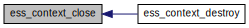
\includegraphics[width=321pt]{dc/d43/ess__context_8c_a9a12468e0f826cc92385be2df34a38d4_icgraph}
\end{center}
\end{figure}
\mbox{\Hypertarget{ess__context_8c_ac764fbb6b72712d2b755f54c6b240e33}\label{ess__context_8c_ac764fbb6b72712d2b755f54c6b240e33}} 
\index{ess\+\_\+context.\+c@{ess\+\_\+context.\+c}!ess\+\_\+context\+\_\+create@{ess\+\_\+context\+\_\+create}}
\index{ess\+\_\+context\+\_\+create@{ess\+\_\+context\+\_\+create}!ess\+\_\+context.\+c@{ess\+\_\+context.\+c}}
\subsubsection{\texorpdfstring{ess\+\_\+context\+\_\+create()}{ess\_context\_create()}}
{\footnotesize\ttfamily \hyperlink{ess__context_8h_acc807999e4f53d1867abf8a0ac682f33}{ess\+\_\+context\+\_\+error\+\_\+t} ess\+\_\+context\+\_\+create (\begin{DoxyParamCaption}\item[{\hyperlink{ess__context_8h_a8a8fec5766c0b3615f8f12f7948e949b}{ess\+\_\+context\+\_\+t} $\ast$}]{context,  }\item[{const \hyperlink{ess__format_8h_ab03f24cb5d42f4448f713bf1ec178163}{ess\+\_\+format\+\_\+t}}]{format }\end{DoxyParamCaption})}



creater the context 


\begin{DoxyCode}
\hyperlink{structess__context}{ess\_context\_t} context;
\hyperlink{ess__context_8h_ac764fbb6b72712d2b755f54c6b240e33}{ess\_context\_create}(&context, ESS\_FORMAT\_STEREO\_92000\_24);
\end{DoxyCode}
 
\begin{DoxyParams}{Parameters}
{\em context} & the context \\
\hline
{\em format} & the using context format \\
\hline
\end{DoxyParams}


Definition at line 38 of file ess\+\_\+context.\+c.


\begin{DoxyCode}
38                                                                                           \{
39   context = (\hyperlink{structess__context}{ess\_context\_t}*)malloc(\textcolor{keyword}{sizeof}(\hyperlink{structess__context}{ess\_context\_t}));
40   \textcolor{keywordflow}{if}(context == 0) \{ context->\hyperlink{structess__context_a7a8b9bb3789092b56f6a6623888fcc3d}{last\_error} = \hyperlink{ess__context_8h_a4b185bc84680674eb2efc8f720d3362ba020750f30895b9adb7b2814810976de0}{ESS\_CONTEXT\_ERROR\_OUTOFMEM};
41     \textcolor{keywordflow}{return} \hyperlink{ess__context_8h_a4b185bc84680674eb2efc8f720d3362ba020750f30895b9adb7b2814810976de0}{ESS\_CONTEXT\_ERROR\_OUTOFMEM}; \}
42 
43   context->\hyperlink{structess__context_abb4395d1c05d3bbc2e1d011507ddd19b}{format} = format;
44   context->\hyperlink{structess__context_a6151ccede5aaf683375710d2677c74c7}{status} = \hyperlink{ess__context_8h_a55313861d12b8c596371cace86eacc2ea2ee2157354733689af9991d071d24d24}{ESS\_CONTEXT\_STATUS\_CREATED};
45   context->\hyperlink{structess__context_a7a8b9bb3789092b56f6a6623888fcc3d}{last\_error} = \hyperlink{ess__context_8h_a4b185bc84680674eb2efc8f720d3362ba5fbe734224f5adb51e59c6dd88506d60}{ESS\_CONTEXT\_ERROR\_OK};
46   \textcolor{keywordflow}{return} \hyperlink{ess__context_8h_a4b185bc84680674eb2efc8f720d3362ba5fbe734224f5adb51e59c6dd88506d60}{ESS\_CONTEXT\_ERROR\_OK};
47 \}
\end{DoxyCode}
\mbox{\Hypertarget{ess__context_8c_a0a9e96c03cba2bfef2999c0199070d17}\label{ess__context_8c_a0a9e96c03cba2bfef2999c0199070d17}} 
\index{ess\+\_\+context.\+c@{ess\+\_\+context.\+c}!ess\+\_\+context\+\_\+destroy@{ess\+\_\+context\+\_\+destroy}}
\index{ess\+\_\+context\+\_\+destroy@{ess\+\_\+context\+\_\+destroy}!ess\+\_\+context.\+c@{ess\+\_\+context.\+c}}
\subsubsection{\texorpdfstring{ess\+\_\+context\+\_\+destroy()}{ess\_context\_destroy()}}
{\footnotesize\ttfamily \hyperlink{ess__context_8h_acc807999e4f53d1867abf8a0ac682f33}{ess\+\_\+context\+\_\+error\+\_\+t} ess\+\_\+context\+\_\+destroy (\begin{DoxyParamCaption}\item[{\hyperlink{ess__context_8h_a8a8fec5766c0b3615f8f12f7948e949b}{ess\+\_\+context\+\_\+t} $\ast$}]{context }\end{DoxyParamCaption})}



destroy and free the context 


\begin{DoxyParams}{Parameters}
{\em context} & the context \\
\hline
\end{DoxyParams}
\begin{DoxyReturn}{Returns}
when ok then E\+S\+S\+\_\+\+C\+O\+N\+T\+E\+X\+T\+\_\+\+E\+R\+R\+O\+R\+\_\+\+OK 
\end{DoxyReturn}


Definition at line 89 of file ess\+\_\+context.\+c.


\begin{DoxyCode}
89                                                                 \{
90   \textcolor{keywordflow}{if}(context == 0) \textcolor{keywordflow}{return} \hyperlink{ess__context_8h_a4b185bc84680674eb2efc8f720d3362baa6ed95d92bbe32c445b0adce2fc256ce}{ESS\_CONTEXT\_ERROR};
91   \hyperlink{ess__context_8c_a9a12468e0f826cc92385be2df34a38d4}{ess\_context\_close}(context);
92   \textcolor{keywordflow}{if}(context->\hyperlink{structess__context_a1fdb06c6d95c1f47d692da94aaf8af17}{backend} != 0) free(context->\hyperlink{structess__context_a1fdb06c6d95c1f47d692da94aaf8af17}{backend} );
93   \textcolor{keywordflow}{if}(context != 0) free(context );
94 
95   context->\hyperlink{structess__context_a7a8b9bb3789092b56f6a6623888fcc3d}{last\_error} = \hyperlink{ess__context_8h_a4b185bc84680674eb2efc8f720d3362ba5fbe734224f5adb51e59c6dd88506d60}{ESS\_CONTEXT\_ERROR\_OK};
96   \textcolor{keywordflow}{return} \hyperlink{ess__context_8h_a4b185bc84680674eb2efc8f720d3362ba5fbe734224f5adb51e59c6dd88506d60}{ESS\_CONTEXT\_ERROR\_OK};
97 \}
\end{DoxyCode}
Here is the call graph for this function\+:\nopagebreak
\begin{figure}[H]
\begin{center}
\leavevmode
\includegraphics[width=321pt]{dc/d43/ess__context_8c_a0a9e96c03cba2bfef2999c0199070d17_cgraph}
\end{center}
\end{figure}
\mbox{\Hypertarget{ess__context_8c_a139494e2518952f79ec0bc7d788d7612}\label{ess__context_8c_a139494e2518952f79ec0bc7d788d7612}} 
\index{ess\+\_\+context.\+c@{ess\+\_\+context.\+c}!ess\+\_\+context\+\_\+get\+\_\+backend\+\_\+info@{ess\+\_\+context\+\_\+get\+\_\+backend\+\_\+info}}
\index{ess\+\_\+context\+\_\+get\+\_\+backend\+\_\+info@{ess\+\_\+context\+\_\+get\+\_\+backend\+\_\+info}!ess\+\_\+context.\+c@{ess\+\_\+context.\+c}}
\subsubsection{\texorpdfstring{ess\+\_\+context\+\_\+get\+\_\+backend\+\_\+info()}{ess\_context\_get\_backend\_info()}}
{\footnotesize\ttfamily const char$\ast$ ess\+\_\+context\+\_\+get\+\_\+backend\+\_\+info (\begin{DoxyParamCaption}\item[{\hyperlink{ess__context_8h_a8a8fec5766c0b3615f8f12f7948e949b}{ess\+\_\+context\+\_\+t} $\ast$}]{context }\end{DoxyParamCaption})}



get using backend informations 


\begin{DoxyParams}{Parameters}
{\em context} & the context \\
\hline
\end{DoxyParams}
\begin{DoxyReturn}{Returns}
the using backend informations 
\end{DoxyReturn}


Definition at line 146 of file ess\+\_\+context.\+c.


\begin{DoxyCode}
146                                                                  \{
147   \textcolor{keywordflow}{if}(context == 0) \textcolor{keywordflow}{return} 0;
148   \textcolor{keywordflow}{return} context->\hyperlink{structess__context_a1fdb06c6d95c1f47d692da94aaf8af17}{backend}->\hyperlink{structess__backend_a9f29adb0a4cfb608557d26692fa78254}{get\_info}();
149 \}
\end{DoxyCode}
\mbox{\Hypertarget{ess__context_8c_a1038af3d90a5a8a45d4fc35cbd425e5b}\label{ess__context_8c_a1038af3d90a5a8a45d4fc35cbd425e5b}} 
\index{ess\+\_\+context.\+c@{ess\+\_\+context.\+c}!ess\+\_\+context\+\_\+get\+\_\+backend\+\_\+name@{ess\+\_\+context\+\_\+get\+\_\+backend\+\_\+name}}
\index{ess\+\_\+context\+\_\+get\+\_\+backend\+\_\+name@{ess\+\_\+context\+\_\+get\+\_\+backend\+\_\+name}!ess\+\_\+context.\+c@{ess\+\_\+context.\+c}}
\subsubsection{\texorpdfstring{ess\+\_\+context\+\_\+get\+\_\+backend\+\_\+name()}{ess\_context\_get\_backend\_name()}}
{\footnotesize\ttfamily const char$\ast$ ess\+\_\+context\+\_\+get\+\_\+backend\+\_\+name (\begin{DoxyParamCaption}\item[{\hyperlink{ess__context_8h_a8a8fec5766c0b3615f8f12f7948e949b}{ess\+\_\+context\+\_\+t} $\ast$}]{context }\end{DoxyParamCaption})}



get the usind backend name 


\begin{DoxyParams}{Parameters}
{\em context} & the context \\
\hline
\end{DoxyParams}
\begin{DoxyReturn}{Returns}
the using backend name 
\end{DoxyReturn}


Definition at line 142 of file ess\+\_\+context.\+c.


\begin{DoxyCode}
142                                                                  \{
143   \textcolor{keywordflow}{if}(context == 0) \textcolor{keywordflow}{return} 0;
144   \textcolor{keywordflow}{return} context->\hyperlink{structess__context_a1fdb06c6d95c1f47d692da94aaf8af17}{backend}->\hyperlink{structess__backend_a1e8975441f4fbb374da179cc7e8bcbae}{get\_name}();
145 \}
\end{DoxyCode}
\mbox{\Hypertarget{ess__context_8c_ae8c078f30231eae2756ff85825dac90a}\label{ess__context_8c_ae8c078f30231eae2756ff85825dac90a}} 
\index{ess\+\_\+context.\+c@{ess\+\_\+context.\+c}!ess\+\_\+context\+\_\+get\+\_\+last\+\_\+error@{ess\+\_\+context\+\_\+get\+\_\+last\+\_\+error}}
\index{ess\+\_\+context\+\_\+get\+\_\+last\+\_\+error@{ess\+\_\+context\+\_\+get\+\_\+last\+\_\+error}!ess\+\_\+context.\+c@{ess\+\_\+context.\+c}}
\subsubsection{\texorpdfstring{ess\+\_\+context\+\_\+get\+\_\+last\+\_\+error()}{ess\_context\_get\_last\_error()}}
{\footnotesize\ttfamily \hyperlink{ess__context_8h_acc807999e4f53d1867abf8a0ac682f33}{ess\+\_\+context\+\_\+error\+\_\+t} ess\+\_\+context\+\_\+get\+\_\+last\+\_\+error (\begin{DoxyParamCaption}\item[{\hyperlink{ess__context_8h_a8a8fec5766c0b3615f8f12f7948e949b}{ess\+\_\+context\+\_\+t} $\ast$}]{context }\end{DoxyParamCaption})}



get the last error from context 


\begin{DoxyParams}{Parameters}
{\em context} & the context \\
\hline
\end{DoxyParams}
\begin{DoxyReturn}{Returns}
the last error 
\end{DoxyReturn}


Definition at line 150 of file ess\+\_\+context.\+c.


\begin{DoxyCode}
150                                                                        \{
151   \textcolor{keywordflow}{if}(context == 0) \textcolor{keywordflow}{return} \hyperlink{ess__context_8h_a4b185bc84680674eb2efc8f720d3362baa6ed95d92bbe32c445b0adce2fc256ce}{ESS\_CONTEXT\_ERROR};
152   \textcolor{keywordflow}{return} context->\hyperlink{structess__context_a7a8b9bb3789092b56f6a6623888fcc3d}{last\_error};
153 \}
\end{DoxyCode}
\mbox{\Hypertarget{ess__context_8c_a40a2211f2793b0346c879b61b35ff63e}\label{ess__context_8c_a40a2211f2793b0346c879b61b35ff63e}} 
\index{ess\+\_\+context.\+c@{ess\+\_\+context.\+c}!ess\+\_\+context\+\_\+init@{ess\+\_\+context\+\_\+init}}
\index{ess\+\_\+context\+\_\+init@{ess\+\_\+context\+\_\+init}!ess\+\_\+context.\+c@{ess\+\_\+context.\+c}}
\subsubsection{\texorpdfstring{ess\+\_\+context\+\_\+init()}{ess\_context\_init()}}
{\footnotesize\ttfamily \hyperlink{ess__context_8h_acc807999e4f53d1867abf8a0ac682f33}{ess\+\_\+context\+\_\+error\+\_\+t} ess\+\_\+context\+\_\+init (\begin{DoxyParamCaption}\item[{\hyperlink{ess__context_8h_a8a8fec5766c0b3615f8f12f7948e949b}{ess\+\_\+context\+\_\+t} $\ast$}]{context,  }\item[{const char $\ast$}]{name }\end{DoxyParamCaption})}



initialisiert the context 


\begin{DoxyCode}
\hyperlink{structess__context}{ess\_context\_t} context;

\hyperlink{ess__context_8h_ac764fbb6b72712d2b755f54c6b240e33}{ess\_context\_create}(&context, ESS\_FORMAT\_STEREO\_92000\_24);
\hyperlink{ess__context_8h_a26ae0093adaa4a6945fed6cfd31d4ae7}{ess\_context\_init\_ex}(&context, \textcolor{stringliteral}{"uart"});
\end{DoxyCode}
 
\begin{DoxyParams}{Parameters}
{\em context} & the context \\
\hline
{\em name} & the name of the using backend \\
\hline
\end{DoxyParams}
\begin{DoxyReturn}{Returns}
when ok then E\+S\+S\+\_\+\+C\+O\+N\+T\+E\+X\+T\+\_\+\+E\+R\+R\+O\+R\+\_\+\+OK 
\end{DoxyReturn}


Definition at line 48 of file ess\+\_\+context.\+c.


\begin{DoxyCode}
48                                                                                \{
49   \textcolor{keywordflow}{if}(context == 0) \textcolor{keywordflow}{return} \hyperlink{ess__context_8h_a4b185bc84680674eb2efc8f720d3362baa6ed95d92bbe32c445b0adce2fc256ce}{ESS\_CONTEXT\_ERROR};
50 
51   \hyperlink{structess__backend}{ess\_backend\_facktory\_t}* backend = 0;
52 
53   \textcolor{keywordflow}{if}(\hyperlink{ess__backend_8h_a9da07e785f1062832e5b0eadae2fd1b1}{ess\_backend\_probe}(name, context->\hyperlink{structess__context_abb4395d1c05d3bbc2e1d011507ddd19b}{format}, backend) == 
      \hyperlink{ess__backend_8h_aac7bdeadfb36709a6f5ab36dda98fb72a4abbaf43c0ba0a394549d3d5394e7545}{ESS\_BACKEND\_OK})
54     \textcolor{keywordflow}{return} \hyperlink{ess__context_8c_a26ae0093adaa4a6945fed6cfd31d4ae7}{ess\_context\_init\_ex}(context, backend);
55   context->\hyperlink{structess__context_a6151ccede5aaf683375710d2677c74c7}{status} = \hyperlink{ess__context_8h_a55313861d12b8c596371cace86eacc2ea6ca265da2cff09e1478d2bdf8d1ebe9b}{ESS\_CONTEXT\_STATUS\_ERROR};
56 
57   \textcolor{keywordflow}{return} \hyperlink{ess__context_8h_a4b185bc84680674eb2efc8f720d3362baa6ed95d92bbe32c445b0adce2fc256ce}{ESS\_CONTEXT\_ERROR};
58 \}
\end{DoxyCode}
Here is the call graph for this function\+:\nopagebreak
\begin{figure}[H]
\begin{center}
\leavevmode
\includegraphics[width=350pt]{dc/d43/ess__context_8c_a40a2211f2793b0346c879b61b35ff63e_cgraph}
\end{center}
\end{figure}
\mbox{\Hypertarget{ess__context_8c_a26ae0093adaa4a6945fed6cfd31d4ae7}\label{ess__context_8c_a26ae0093adaa4a6945fed6cfd31d4ae7}} 
\index{ess\+\_\+context.\+c@{ess\+\_\+context.\+c}!ess\+\_\+context\+\_\+init\+\_\+ex@{ess\+\_\+context\+\_\+init\+\_\+ex}}
\index{ess\+\_\+context\+\_\+init\+\_\+ex@{ess\+\_\+context\+\_\+init\+\_\+ex}!ess\+\_\+context.\+c@{ess\+\_\+context.\+c}}
\subsubsection{\texorpdfstring{ess\+\_\+context\+\_\+init\+\_\+ex()}{ess\_context\_init\_ex()}}
{\footnotesize\ttfamily \hyperlink{ess__context_8h_acc807999e4f53d1867abf8a0ac682f33}{ess\+\_\+context\+\_\+error\+\_\+t} ess\+\_\+context\+\_\+init\+\_\+ex (\begin{DoxyParamCaption}\item[{\hyperlink{ess__context_8h_a8a8fec5766c0b3615f8f12f7948e949b}{ess\+\_\+context\+\_\+t} $\ast$}]{context,  }\item[{\hyperlink{ess__backend_8h_ab1487f8c501b38b66796d0fbecb7ed7b}{ess\+\_\+backend\+\_\+facktory\+\_\+t} $\ast$}]{backend }\end{DoxyParamCaption})}



initialisiert the context with a user backend 


\begin{DoxyCode}
\hyperlink{structess__context}{ess\_context\_t} context;
\hyperlink{structess__backend}{ess\_backend\_facktory\_t}* user\_backend = \{ ,,, \};

\hyperlink{ess__context_8h_ac764fbb6b72712d2b755f54c6b240e33}{ess\_context\_create}(&context, ESS\_FORMAT\_STEREO\_92000\_24);

\hyperlink{ess__context_8h_a26ae0093adaa4a6945fed6cfd31d4ae7}{ess\_context\_init\_ex}(&context, user\_backend);
\end{DoxyCode}
 
\begin{DoxyParams}{Parameters}
{\em context} & the context \\
\hline
\end{DoxyParams}
\begin{DoxyReturn}{Returns}
when ok then E\+S\+S\+\_\+\+C\+O\+N\+T\+E\+X\+T\+\_\+\+E\+R\+R\+O\+R\+\_\+\+OK 
\end{DoxyReturn}


Definition at line 59 of file ess\+\_\+context.\+c.


\begin{DoxyCode}
59                                                                                                  \{
60   \textcolor{keywordflow}{if}(backend == 0 && backend == 0) \{
61     context->\hyperlink{structess__context_a7a8b9bb3789092b56f6a6623888fcc3d}{last\_error} = \hyperlink{ess__context_8h_a4b185bc84680674eb2efc8f720d3362ba29dbe40f674348273f3b23c9c5fcf62d}{ESS\_CONTEXT\_ERRORNOBACKEND};
62     \textcolor{keywordflow}{return} \hyperlink{ess__context_8h_a4b185bc84680674eb2efc8f720d3362ba29dbe40f674348273f3b23c9c5fcf62d}{ESS\_CONTEXT\_ERRORNOBACKEND};
63   \}
64 
65   \textcolor{keywordflow}{if}(backend->\hyperlink{structess__backend_ae6dfe97715fbf9f3fbf7b46a2d311e64}{ess\_backend\_open}(context->\hyperlink{structess__context_abb4395d1c05d3bbc2e1d011507ddd19b}{format}) != 0) \{
66     ESP\_LOGE(\hyperlink{ess__context_8c_a7ce0df38eb467e59f209470c8f5ac4e6}{LOG\_TAG},\textcolor{stringliteral}{"Error to open backend"});
67     \textcolor{keywordflow}{return} -1;
68   \} \textcolor{keywordflow}{else} \{
69 
70     context->\hyperlink{structess__context_a1fdb06c6d95c1f47d692da94aaf8af17}{backend} = backend;
71     context->\hyperlink{structess__context_a6151ccede5aaf683375710d2677c74c7}{status} = \hyperlink{ess__context_8h_a55313861d12b8c596371cace86eacc2eada32323ceb7303d5432781a25cef7f65}{ESS\_CONTEXT\_STATUS\_RUN};
72     
73   \}
74   context->\hyperlink{structess__context_a7a8b9bb3789092b56f6a6623888fcc3d}{last\_error} = \hyperlink{ess__context_8h_a4b185bc84680674eb2efc8f720d3362ba5fbe734224f5adb51e59c6dd88506d60}{ESS\_CONTEXT\_ERROR\_OK};
75   \textcolor{keywordflow}{return} \hyperlink{ess__context_8h_a4b185bc84680674eb2efc8f720d3362ba5fbe734224f5adb51e59c6dd88506d60}{ESS\_CONTEXT\_ERROR\_OK};
76 \}
\end{DoxyCode}
Here is the caller graph for this function\+:\nopagebreak
\begin{figure}[H]
\begin{center}
\leavevmode
\includegraphics[width=308pt]{dc/d43/ess__context_8c_a26ae0093adaa4a6945fed6cfd31d4ae7_icgraph}
\end{center}
\end{figure}
\mbox{\Hypertarget{ess__context_8c_a6b450cd4cfd4fed931f99b05c38e0172}\label{ess__context_8c_a6b450cd4cfd4fed931f99b05c38e0172}} 
\index{ess\+\_\+context.\+c@{ess\+\_\+context.\+c}!ess\+\_\+context\+\_\+paused@{ess\+\_\+context\+\_\+paused}}
\index{ess\+\_\+context\+\_\+paused@{ess\+\_\+context\+\_\+paused}!ess\+\_\+context.\+c@{ess\+\_\+context.\+c}}
\subsubsection{\texorpdfstring{ess\+\_\+context\+\_\+paused()}{ess\_context\_paused()}}
{\footnotesize\ttfamily \hyperlink{ess__context_8h_acc807999e4f53d1867abf8a0ac682f33}{ess\+\_\+context\+\_\+error\+\_\+t} ess\+\_\+context\+\_\+paused (\begin{DoxyParamCaption}\item[{\hyperlink{ess__context_8h_a8a8fec5766c0b3615f8f12f7948e949b}{ess\+\_\+context\+\_\+t} $\ast$}]{context }\end{DoxyParamCaption})}



set backend to standby 


\begin{DoxyParams}{Parameters}
{\em context} & the context \\
\hline
\end{DoxyParams}
\begin{DoxyReturn}{Returns}
when ok then E\+S\+S\+\_\+\+C\+O\+N\+T\+E\+X\+T\+\_\+\+E\+R\+R\+O\+R\+\_\+\+OK 
\end{DoxyReturn}


Definition at line 99 of file ess\+\_\+context.\+c.


\begin{DoxyCode}
99                                                                \{
100   \textcolor{keywordflow}{if}(context == 0) \textcolor{keywordflow}{return} \hyperlink{ess__context_8h_a4b185bc84680674eb2efc8f720d3362baa6ed95d92bbe32c445b0adce2fc256ce}{ESS\_CONTEXT\_ERROR};
101   \textcolor{keywordflow}{if}(context->\hyperlink{structess__context_a1fdb06c6d95c1f47d692da94aaf8af17}{backend} == 0)  \textcolor{keywordflow}{return} context->\hyperlink{structess__context_a7a8b9bb3789092b56f6a6623888fcc3d}{last\_error} =  
      \hyperlink{ess__context_8h_a4b185bc84680674eb2efc8f720d3362ba29dbe40f674348273f3b23c9c5fcf62d}{ESS\_CONTEXT\_ERRORNOBACKEND};
102 
103   context->\hyperlink{structess__context_a6151ccede5aaf683375710d2677c74c7}{status} = \hyperlink{ess__context_8h_a55313861d12b8c596371cace86eacc2ea6f6315ef32fd6f85789578726d3d06b9}{ESS\_CONTEXT\_STATUS\_PAUSED};
104   context->\hyperlink{structess__context_a1fdb06c6d95c1f47d692da94aaf8af17}{backend}->\hyperlink{structess__backend_ad263ce89d932658c73be2e5863d0afcf}{ess\_backend\_pause}();
105 
106   context->\hyperlink{structess__context_a7a8b9bb3789092b56f6a6623888fcc3d}{last\_error} = \hyperlink{ess__context_8h_a4b185bc84680674eb2efc8f720d3362ba5fbe734224f5adb51e59c6dd88506d60}{ESS\_CONTEXT\_ERROR\_OK};
107   \textcolor{keywordflow}{return} \hyperlink{ess__context_8h_a4b185bc84680674eb2efc8f720d3362ba5fbe734224f5adb51e59c6dd88506d60}{ESS\_CONTEXT\_ERROR\_OK};
108 \}
\end{DoxyCode}
\mbox{\Hypertarget{ess__context_8c_ac6041313862e70f48b8441df8136b0ba}\label{ess__context_8c_ac6041313862e70f48b8441df8136b0ba}} 
\index{ess\+\_\+context.\+c@{ess\+\_\+context.\+c}!ess\+\_\+context\+\_\+resume@{ess\+\_\+context\+\_\+resume}}
\index{ess\+\_\+context\+\_\+resume@{ess\+\_\+context\+\_\+resume}!ess\+\_\+context.\+c@{ess\+\_\+context.\+c}}
\subsubsection{\texorpdfstring{ess\+\_\+context\+\_\+resume()}{ess\_context\_resume()}}
{\footnotesize\ttfamily \hyperlink{ess__context_8h_acc807999e4f53d1867abf8a0ac682f33}{ess\+\_\+context\+\_\+error\+\_\+t} ess\+\_\+context\+\_\+resume (\begin{DoxyParamCaption}\item[{\hyperlink{ess__context_8h_a8a8fec5766c0b3615f8f12f7948e949b}{ess\+\_\+context\+\_\+t} $\ast$}]{context }\end{DoxyParamCaption})}



set backend to run 


\begin{DoxyParams}{Parameters}
{\em context} & the context \\
\hline
\end{DoxyParams}
\begin{DoxyReturn}{Returns}
when ok then E\+S\+S\+\_\+\+C\+O\+N\+T\+E\+X\+T\+\_\+\+E\+R\+R\+O\+R\+\_\+\+OK 
\end{DoxyReturn}


Definition at line 109 of file ess\+\_\+context.\+c.


\begin{DoxyCode}
109                                                                \{
110   \textcolor{keywordflow}{if}(context == 0) \textcolor{keywordflow}{return} \hyperlink{ess__context_8h_a4b185bc84680674eb2efc8f720d3362baa6ed95d92bbe32c445b0adce2fc256ce}{ESS\_CONTEXT\_ERROR};
111   \textcolor{keywordflow}{if}(context->\hyperlink{structess__context_a1fdb06c6d95c1f47d692da94aaf8af17}{backend} == 0)  \textcolor{keywordflow}{return} context->\hyperlink{structess__context_a7a8b9bb3789092b56f6a6623888fcc3d}{last\_error} =  
      \hyperlink{ess__context_8h_a4b185bc84680674eb2efc8f720d3362ba29dbe40f674348273f3b23c9c5fcf62d}{ESS\_CONTEXT\_ERRORNOBACKEND};
112 
113   context->\hyperlink{structess__context_a6151ccede5aaf683375710d2677c74c7}{status} = \hyperlink{ess__context_8h_a55313861d12b8c596371cace86eacc2eada32323ceb7303d5432781a25cef7f65}{ESS\_CONTEXT\_STATUS\_RUN};
114   context->\hyperlink{structess__context_a1fdb06c6d95c1f47d692da94aaf8af17}{backend}->\hyperlink{structess__backend_ab9a30f8d9f4bd941ae74e3ef0c9d7aa3}{ess\_backend\_resum}();
115 
116   context->\hyperlink{structess__context_a7a8b9bb3789092b56f6a6623888fcc3d}{last\_error} = \hyperlink{ess__context_8h_a4b185bc84680674eb2efc8f720d3362ba5fbe734224f5adb51e59c6dd88506d60}{ESS\_CONTEXT\_ERROR\_OK};
117   \textcolor{keywordflow}{return} \hyperlink{ess__context_8h_a4b185bc84680674eb2efc8f720d3362ba5fbe734224f5adb51e59c6dd88506d60}{ESS\_CONTEXT\_ERROR\_OK};
118 \}
\end{DoxyCode}
\mbox{\Hypertarget{ess__context_8c_aebeaf3ec64fe0e348557884dfa601944}\label{ess__context_8c_aebeaf3ec64fe0e348557884dfa601944}} 
\index{ess\+\_\+context.\+c@{ess\+\_\+context.\+c}!ess\+\_\+context\+\_\+set\+\_\+format@{ess\+\_\+context\+\_\+set\+\_\+format}}
\index{ess\+\_\+context\+\_\+set\+\_\+format@{ess\+\_\+context\+\_\+set\+\_\+format}!ess\+\_\+context.\+c@{ess\+\_\+context.\+c}}
\subsubsection{\texorpdfstring{ess\+\_\+context\+\_\+set\+\_\+format()}{ess\_context\_set\_format()}}
{\footnotesize\ttfamily \hyperlink{ess__context_8h_acc807999e4f53d1867abf8a0ac682f33}{ess\+\_\+context\+\_\+error\+\_\+t} ess\+\_\+context\+\_\+set\+\_\+format (\begin{DoxyParamCaption}\item[{\hyperlink{ess__context_8h_a8a8fec5766c0b3615f8f12f7948e949b}{ess\+\_\+context\+\_\+t} $\ast$}]{context,  }\item[{const \hyperlink{ess__format_8h_ab03f24cb5d42f4448f713bf1ec178163}{ess\+\_\+format\+\_\+t}}]{format }\end{DoxyParamCaption})}



set the sample format to backend 


\begin{DoxyParams}{Parameters}
{\em context} & the context 
\begin{DoxyCode}
\hyperlink{structess__context}{ess\_context\_t} context;

\hyperlink{ess__context_8h_ac764fbb6b72712d2b755f54c6b240e33}{ess\_context\_create}(&context, ESS\_FORMAT\_STEREO\_92000\_24); \textcolor{comment}{// Backend Format}
\hyperlink{ess__context_8h_a26ae0093adaa4a6945fed6cfd31d4ae7}{ess\_context\_init\_ex}(&context, \textcolor{stringliteral}{"uart"}); \textcolor{comment}{// open uart backend}

\hyperlink{ess__context_8h_aebeaf3ec64fe0e348557884dfa601944}{ess\_context\_set\_format}(&context, LOADED\_WAV\_FORMAT);
\end{DoxyCode}
 \\
\hline
{\em format} & the new using format \\
\hline
\end{DoxyParams}
\begin{DoxyReturn}{Returns}
when ok then E\+S\+S\+\_\+\+C\+O\+N\+T\+E\+X\+T\+\_\+\+E\+R\+R\+O\+R\+\_\+\+OK 
\end{DoxyReturn}


Definition at line 120 of file ess\+\_\+context.\+c.


\begin{DoxyCode}
120                                                                                               \{
121   \textcolor{keywordflow}{if}(context == 0) \textcolor{keywordflow}{return} \hyperlink{ess__context_8h_a4b185bc84680674eb2efc8f720d3362baa6ed95d92bbe32c445b0adce2fc256ce}{ESS\_CONTEXT\_ERROR};
122   \textcolor{keywordflow}{if}(context->\hyperlink{structess__context_a1fdb06c6d95c1f47d692da94aaf8af17}{backend} == 0)  \textcolor{keywordflow}{return} context->\hyperlink{structess__context_a7a8b9bb3789092b56f6a6623888fcc3d}{last\_error} =  
      \hyperlink{ess__context_8h_a4b185bc84680674eb2efc8f720d3362ba29dbe40f674348273f3b23c9c5fcf62d}{ESS\_CONTEXT\_ERRORNOBACKEND};
123 
124   \textcolor{keywordflow}{return} (\hyperlink{ess__backend_8h_ab9b737a43ebfa9d220c02a32e79346d8}{ess\_backend\_set\_sample\_format}(context->
      \hyperlink{structess__context_a1fdb06c6d95c1f47d692da94aaf8af17}{backend}, format) != 0) ? \hyperlink{ess__context_8h_a4b185bc84680674eb2efc8f720d3362bace646ce156ae1461491206d2bfa7f902}{ESS\_CONTEXT\_WRONGFORMAT} : 
      \hyperlink{ess__context_8h_a4b185bc84680674eb2efc8f720d3362ba5fbe734224f5adb51e59c6dd88506d60}{ESS\_CONTEXT\_ERROR\_OK};
125 \}
\end{DoxyCode}
Here is the call graph for this function\+:\nopagebreak
\begin{figure}[H]
\begin{center}
\leavevmode
\includegraphics[width=350pt]{dc/d43/ess__context_8c_aebeaf3ec64fe0e348557884dfa601944_cgraph}
\end{center}
\end{figure}
\mbox{\Hypertarget{ess__context_8c_ae2c6a4e2f8a5128fc1bb05afea5f3c8d}\label{ess__context_8c_ae2c6a4e2f8a5128fc1bb05afea5f3c8d}} 
\index{ess\+\_\+context.\+c@{ess\+\_\+context.\+c}!ess\+\_\+context\+\_\+write@{ess\+\_\+context\+\_\+write}}
\index{ess\+\_\+context\+\_\+write@{ess\+\_\+context\+\_\+write}!ess\+\_\+context.\+c@{ess\+\_\+context.\+c}}
\subsubsection{\texorpdfstring{ess\+\_\+context\+\_\+write()}{ess\_context\_write()}}
{\footnotesize\ttfamily unsigned int ess\+\_\+context\+\_\+write (\begin{DoxyParamCaption}\item[{\hyperlink{ess__context_8h_a8a8fec5766c0b3615f8f12f7948e949b}{ess\+\_\+context\+\_\+t} $\ast$}]{context,  }\item[{void $\ast$}]{buffer,  }\item[{unsigned int}]{buf\+\_\+size }\end{DoxyParamCaption})}



write audio data to the backend 


\begin{DoxyParams}{Parameters}
{\em context} & the context \\
\hline
{\em buffer} & the audio pcm data \\
\hline
{\em buf\+\_\+size} & the size of the buffer \\
\hline
\end{DoxyParams}
\begin{DoxyReturn}{Returns}
the written data. 
\end{DoxyReturn}


Definition at line 127 of file ess\+\_\+context.\+c.


\begin{DoxyCode}
127                                                                                             \{
128   \textcolor{keywordtype}{unsigned} \textcolor{keywordtype}{int} wrote;
129   \hyperlink{ess__context_8c_a8077482da675241fd832152974033994}{ess\_context\_write\_ex}(context, buffer, buf\_size, &wrote);
130   \textcolor{keywordflow}{return} wrote;
131 \}
\end{DoxyCode}
Here is the call graph for this function\+:\nopagebreak
\begin{figure}[H]
\begin{center}
\leavevmode
\includegraphics[width=324pt]{dc/d43/ess__context_8c_ae2c6a4e2f8a5128fc1bb05afea5f3c8d_cgraph}
\end{center}
\end{figure}
\mbox{\Hypertarget{ess__context_8c_a8077482da675241fd832152974033994}\label{ess__context_8c_a8077482da675241fd832152974033994}} 
\index{ess\+\_\+context.\+c@{ess\+\_\+context.\+c}!ess\+\_\+context\+\_\+write\+\_\+ex@{ess\+\_\+context\+\_\+write\+\_\+ex}}
\index{ess\+\_\+context\+\_\+write\+\_\+ex@{ess\+\_\+context\+\_\+write\+\_\+ex}!ess\+\_\+context.\+c@{ess\+\_\+context.\+c}}
\subsubsection{\texorpdfstring{ess\+\_\+context\+\_\+write\+\_\+ex()}{ess\_context\_write\_ex()}}
{\footnotesize\ttfamily \hyperlink{ess__context_8h_acc807999e4f53d1867abf8a0ac682f33}{ess\+\_\+context\+\_\+error\+\_\+t} ess\+\_\+context\+\_\+write\+\_\+ex (\begin{DoxyParamCaption}\item[{\hyperlink{ess__context_8h_a8a8fec5766c0b3615f8f12f7948e949b}{ess\+\_\+context\+\_\+t} $\ast$}]{context,  }\item[{void $\ast$}]{buffer,  }\item[{unsigned int}]{buf\+\_\+size,  }\item[{unsigned int $\ast$}]{wrote }\end{DoxyParamCaption})}



write audio data to the backend 


\begin{DoxyParams}{Parameters}
{\em context} & the context \\
\hline
{\em buffer} & the audio pcm data \\
\hline
{\em buf\+\_\+size} & the size of the buffer \\
\hline
{\em wrote} & the written data \\
\hline
\end{DoxyParams}
\begin{DoxyReturn}{Returns}
when ok then E\+S\+S\+\_\+\+C\+O\+N\+T\+E\+X\+T\+\_\+\+E\+R\+R\+O\+R\+\_\+\+OK 
\end{DoxyReturn}


Definition at line 132 of file ess\+\_\+context.\+c.


\begin{DoxyCode}
132                                                                                                            
                       \{
133   \textcolor{keywordflow}{if}(context == 0) \textcolor{keywordflow}{return} \hyperlink{ess__context_8h_a4b185bc84680674eb2efc8f720d3362baa6ed95d92bbe32c445b0adce2fc256ce}{ESS\_CONTEXT\_ERROR};
134   \textcolor{keywordflow}{if}(context->\hyperlink{structess__context_a6151ccede5aaf683375710d2677c74c7}{status} == \hyperlink{ess__context_8h_a55313861d12b8c596371cace86eacc2ea6f6315ef32fd6f85789578726d3d06b9}{ESS\_CONTEXT\_STATUS\_PAUSED}) \textcolor{keywordflow}{return} context->
      \hyperlink{structess__context_a7a8b9bb3789092b56f6a6623888fcc3d}{last\_error} = \hyperlink{ess__context_8h_a4b185bc84680674eb2efc8f720d3362baf33b77dd00f57d9dd7ab4909e3559dae}{ESS\_CONTEX\_ISPAUSED};
135   \textcolor{keywordflow}{if}(context->\hyperlink{structess__context_a1fdb06c6d95c1f47d692da94aaf8af17}{backend} == 0)  \textcolor{keywordflow}{return} context->\hyperlink{structess__context_a7a8b9bb3789092b56f6a6623888fcc3d}{last\_error} =  
      \hyperlink{ess__context_8h_a4b185bc84680674eb2efc8f720d3362ba29dbe40f674348273f3b23c9c5fcf62d}{ESS\_CONTEXT\_ERRORNOBACKEND};
136 
137   context->\hyperlink{structess__context_a1fdb06c6d95c1f47d692da94aaf8af17}{backend}->\hyperlink{structess__backend_a3a1b32830c82ec84aa0e6c02280d7f6c}{ess\_backend\_write}(buffer, buf\_size, wrote);
138 
139   \textcolor{keywordflow}{return}  \hyperlink{ess__context_8h_a4b185bc84680674eb2efc8f720d3362ba5fbe734224f5adb51e59c6dd88506d60}{ESS\_CONTEXT\_ERROR\_OK};
140 \}
\end{DoxyCode}
Here is the caller graph for this function\+:\nopagebreak
\begin{figure}[H]
\begin{center}
\leavevmode
\includegraphics[width=324pt]{dc/d43/ess__context_8c_a8077482da675241fd832152974033994_icgraph}
\end{center}
\end{figure}

\hypertarget{ess__format_8c}{}\section{src/ess\+\_\+format.c File Reference}
\label{ess__format_8c}\index{src/ess\+\_\+format.\+c@{src/ess\+\_\+format.\+c}}
{\ttfamily \#include \char`\"{}ess\+\_\+format.\+h\char`\"{}}\newline
{\ttfamily \#include $<$stdio.\+h$>$}\newline
Include dependency graph for ess\+\_\+format.\+c\+:
\nopagebreak
\begin{figure}[H]
\begin{center}
\leavevmode
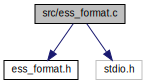
\includegraphics[width=218pt]{d0/d52/ess__format_8c__incl}
\end{center}
\end{figure}
\subsection*{Data Structures}
\begin{DoxyCompactItemize}
\item 
struct \hyperlink{struct__format2human}{\+\_\+format2human}
\end{DoxyCompactItemize}
\subsection*{Typedefs}
\begin{DoxyCompactItemize}
\item 
typedef struct \hyperlink{struct__format2human}{\+\_\+format2human} \hyperlink{ess__format_8c_a4f7127cfbaa16ee8a1e6449a9b6e3325}{format2human\+\_\+t}
\end{DoxyCompactItemize}
\subsection*{Functions}
\begin{DoxyCompactItemize}
\item 
int \hyperlink{ess__format_8c_af1af5721aa4c3a136fef2b5eec4e5a91}{ess\+\_\+format\+\_\+get\+\_\+channels} (const \hyperlink{ess__format_8h_ab03f24cb5d42f4448f713bf1ec178163}{ess\+\_\+format\+\_\+t} format)
\begin{DoxyCompactList}\small\item\em Help to get the number of channels of the format. \end{DoxyCompactList}\item 
int \hyperlink{ess__format_8c_a8a38ecc33aa70a8f9497d350706b6463}{ess\+\_\+format\+\_\+get\+\_\+samplerate} (const \hyperlink{ess__format_8h_ab03f24cb5d42f4448f713bf1ec178163}{ess\+\_\+format\+\_\+t} format)
\begin{DoxyCompactList}\small\item\em Help to get the samplerate of the format. \end{DoxyCompactList}\item 
int \hyperlink{ess__format_8c_a57f133a9941097d8edc520a1769f0b16}{ess\+\_\+format\+\_\+get\+\_\+bits} (const \hyperlink{ess__format_8h_ab03f24cb5d42f4448f713bf1ec178163}{ess\+\_\+format\+\_\+t} format)
\begin{DoxyCompactList}\small\item\em Help to get bits of the format. \end{DoxyCompactList}\item 
const char $\ast$ \hyperlink{ess__format_8c_add94d3ae146eb3612217c1d8cceaa0a4}{ess\+\_\+format\+\_\+to\+\_\+string} (\hyperlink{ess__format_8h_ab03f24cb5d42f4448f713bf1ec178163}{ess\+\_\+format\+\_\+t} format)
\begin{DoxyCompactList}\small\item\em Help to get the string of the format. \end{DoxyCompactList}\end{DoxyCompactItemize}
\subsection*{Variables}
\begin{DoxyCompactItemize}
\item 
\hyperlink{ess__format_8c_a4f7127cfbaa16ee8a1e6449a9b6e3325}{format2human\+\_\+t} \hyperlink{ess__format_8c_afe86278e648eeb366ddc31cb864ec547}{format\+\_\+parse} \mbox{[}$\,$\mbox{]}
\end{DoxyCompactItemize}


\subsection{Typedef Documentation}
\mbox{\Hypertarget{ess__format_8c_a4f7127cfbaa16ee8a1e6449a9b6e3325}\label{ess__format_8c_a4f7127cfbaa16ee8a1e6449a9b6e3325}} 
\index{ess\+\_\+format.\+c@{ess\+\_\+format.\+c}!format2human\+\_\+t@{format2human\+\_\+t}}
\index{format2human\+\_\+t@{format2human\+\_\+t}!ess\+\_\+format.\+c@{ess\+\_\+format.\+c}}
\subsubsection{\texorpdfstring{format2human\+\_\+t}{format2human\_t}}
{\footnotesize\ttfamily typedef struct \hyperlink{struct__format2human}{\+\_\+format2human} \hyperlink{ess__format_8c_a4f7127cfbaa16ee8a1e6449a9b6e3325}{format2human\+\_\+t}}



\subsection{Function Documentation}
\mbox{\Hypertarget{ess__format_8c_a57f133a9941097d8edc520a1769f0b16}\label{ess__format_8c_a57f133a9941097d8edc520a1769f0b16}} 
\index{ess\+\_\+format.\+c@{ess\+\_\+format.\+c}!ess\+\_\+format\+\_\+get\+\_\+bits@{ess\+\_\+format\+\_\+get\+\_\+bits}}
\index{ess\+\_\+format\+\_\+get\+\_\+bits@{ess\+\_\+format\+\_\+get\+\_\+bits}!ess\+\_\+format.\+c@{ess\+\_\+format.\+c}}
\subsubsection{\texorpdfstring{ess\+\_\+format\+\_\+get\+\_\+bits()}{ess\_format\_get\_bits()}}
{\footnotesize\ttfamily int ess\+\_\+format\+\_\+get\+\_\+bits (\begin{DoxyParamCaption}\item[{const \hyperlink{ess__format_8h_ab03f24cb5d42f4448f713bf1ec178163}{ess\+\_\+format\+\_\+t}}]{format }\end{DoxyParamCaption})}



Help to get bits of the format. 


\begin{DoxyParams}{Parameters}
{\em format} & The format to parse \\
\hline
\end{DoxyParams}


Definition at line 68 of file ess\+\_\+format.\+c.


\begin{DoxyCode}
68                                                    \{
69   \textcolor{keywordflow}{if}(format >= \hyperlink{ess__format_8h_afd7aa3f758b1c34994d1fe911d8365b6}{ESS\_FORMAT\_MAX}) \textcolor{keywordflow}{return} -1;
70   \textcolor{keywordflow}{return} \hyperlink{ess__format_8c_afe86278e648eeb366ddc31cb864ec547}{format\_parse}[format].\hyperlink{struct__format2human_ad1e28a1a66a25529b0b61b9ca4e66d44}{bits};
71 \}
\end{DoxyCode}
\mbox{\Hypertarget{ess__format_8c_af1af5721aa4c3a136fef2b5eec4e5a91}\label{ess__format_8c_af1af5721aa4c3a136fef2b5eec4e5a91}} 
\index{ess\+\_\+format.\+c@{ess\+\_\+format.\+c}!ess\+\_\+format\+\_\+get\+\_\+channels@{ess\+\_\+format\+\_\+get\+\_\+channels}}
\index{ess\+\_\+format\+\_\+get\+\_\+channels@{ess\+\_\+format\+\_\+get\+\_\+channels}!ess\+\_\+format.\+c@{ess\+\_\+format.\+c}}
\subsubsection{\texorpdfstring{ess\+\_\+format\+\_\+get\+\_\+channels()}{ess\_format\_get\_channels()}}
{\footnotesize\ttfamily int ess\+\_\+format\+\_\+get\+\_\+channels (\begin{DoxyParamCaption}\item[{const \hyperlink{ess__format_8h_ab03f24cb5d42f4448f713bf1ec178163}{ess\+\_\+format\+\_\+t}}]{format }\end{DoxyParamCaption})}



Help to get the number of channels of the format. 


\begin{DoxyParams}{Parameters}
{\em format} & The format to parse \\
\hline
\end{DoxyParams}


Definition at line 59 of file ess\+\_\+format.\+c.


\begin{DoxyCode}
59                                                        \{
60   \textcolor{keywordflow}{if}(format >= \hyperlink{ess__format_8h_afd7aa3f758b1c34994d1fe911d8365b6}{ESS\_FORMAT\_MAX}) \textcolor{keywordflow}{return} -1;
61     \textcolor{keywordflow}{return} \hyperlink{ess__format_8c_afe86278e648eeb366ddc31cb864ec547}{format\_parse}[format].\hyperlink{struct__format2human_a178795099d0608972755dfef8d8367e3}{channels};
62 \}
\end{DoxyCode}
\mbox{\Hypertarget{ess__format_8c_a8a38ecc33aa70a8f9497d350706b6463}\label{ess__format_8c_a8a38ecc33aa70a8f9497d350706b6463}} 
\index{ess\+\_\+format.\+c@{ess\+\_\+format.\+c}!ess\+\_\+format\+\_\+get\+\_\+samplerate@{ess\+\_\+format\+\_\+get\+\_\+samplerate}}
\index{ess\+\_\+format\+\_\+get\+\_\+samplerate@{ess\+\_\+format\+\_\+get\+\_\+samplerate}!ess\+\_\+format.\+c@{ess\+\_\+format.\+c}}
\subsubsection{\texorpdfstring{ess\+\_\+format\+\_\+get\+\_\+samplerate()}{ess\_format\_get\_samplerate()}}
{\footnotesize\ttfamily int ess\+\_\+format\+\_\+get\+\_\+samplerate (\begin{DoxyParamCaption}\item[{const \hyperlink{ess__format_8h_ab03f24cb5d42f4448f713bf1ec178163}{ess\+\_\+format\+\_\+t}}]{format }\end{DoxyParamCaption})}



Help to get the samplerate of the format. 


\begin{DoxyParams}{Parameters}
{\em format} & The format to parse \\
\hline
\end{DoxyParams}


Definition at line 63 of file ess\+\_\+format.\+c.


\begin{DoxyCode}
63                                                          \{
64   \textcolor{keywordflow}{if}(format >= \hyperlink{ess__format_8h_afd7aa3f758b1c34994d1fe911d8365b6}{ESS\_FORMAT\_MAX}) \textcolor{keywordflow}{return} -1;
65   \textcolor{keywordflow}{return} \hyperlink{ess__format_8c_afe86278e648eeb366ddc31cb864ec547}{format\_parse}[format].\hyperlink{struct__format2human_ac38751c7169cfeb9325a947cc0484286}{samplerate};
66 \}
\end{DoxyCode}
\mbox{\Hypertarget{ess__format_8c_add94d3ae146eb3612217c1d8cceaa0a4}\label{ess__format_8c_add94d3ae146eb3612217c1d8cceaa0a4}} 
\index{ess\+\_\+format.\+c@{ess\+\_\+format.\+c}!ess\+\_\+format\+\_\+to\+\_\+string@{ess\+\_\+format\+\_\+to\+\_\+string}}
\index{ess\+\_\+format\+\_\+to\+\_\+string@{ess\+\_\+format\+\_\+to\+\_\+string}!ess\+\_\+format.\+c@{ess\+\_\+format.\+c}}
\subsubsection{\texorpdfstring{ess\+\_\+format\+\_\+to\+\_\+string()}{ess\_format\_to\_string()}}
{\footnotesize\ttfamily const char$\ast$ ess\+\_\+format\+\_\+to\+\_\+string (\begin{DoxyParamCaption}\item[{const \hyperlink{ess__format_8h_ab03f24cb5d42f4448f713bf1ec178163}{ess\+\_\+format\+\_\+t}}]{format }\end{DoxyParamCaption})}



Help to get the string of the format. 


\begin{DoxyParams}{Parameters}
{\em format} & The format to parse \\
\hline
\end{DoxyParams}


Definition at line 76 of file ess\+\_\+format.\+c.


\begin{DoxyCode}
76                                                       \{
77   \textcolor{keywordflow}{if}(format >= \hyperlink{ess__format_8h_afd7aa3f758b1c34994d1fe911d8365b6}{ESS\_FORMAT\_MAX}) \textcolor{keywordflow}{return} \textcolor{stringliteral}{"NO\_FORMAT"};
78   \textcolor{keywordflow}{return} \hyperlink{ess__format_8c_afe86278e648eeb366ddc31cb864ec547}{format\_parse}[format].\hyperlink{struct__format2human_a14f2551e7b5032527b89aa2d4025523a}{string};
79   \textcolor{keywordflow}{return} \textcolor{stringliteral}{"NO\_FORMAT"};
80 \}
\end{DoxyCode}
Here is the caller graph for this function\+:
\nopagebreak
\begin{figure}[H]
\begin{center}
\leavevmode
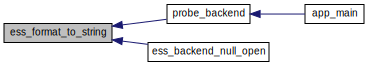
\includegraphics[width=348pt]{de/d96/ess__format_8c_add94d3ae146eb3612217c1d8cceaa0a4_icgraph}
\end{center}
\end{figure}


\subsection{Variable Documentation}
\mbox{\Hypertarget{ess__format_8c_afe86278e648eeb366ddc31cb864ec547}\label{ess__format_8c_afe86278e648eeb366ddc31cb864ec547}} 
\index{ess\+\_\+format.\+c@{ess\+\_\+format.\+c}!format\+\_\+parse@{format\+\_\+parse}}
\index{format\+\_\+parse@{format\+\_\+parse}!ess\+\_\+format.\+c@{ess\+\_\+format.\+c}}
\subsubsection{\texorpdfstring{format\+\_\+parse}{format\_parse}}
{\footnotesize\ttfamily \hyperlink{ess__format_8c_a4f7127cfbaa16ee8a1e6449a9b6e3325}{format2human\+\_\+t} format\+\_\+parse\mbox{[}$\,$\mbox{]}}

{\bfseries Initial value\+:}
\begin{DoxyCode}
= \{
  \{  \textcolor{stringliteral}{"ESS\_FORMAT\_MONO\_44100\_8"}, 44100, 8, 1 \},
  \{  \textcolor{stringliteral}{"ESS\_FORMAT\_MONO\_48000\_8"}, 48000, 8, 1 \},
  \{  \textcolor{stringliteral}{"ESS\_FORMAT\_MONO\_96000\_8"}, 96000, 8, 1 \},
  \{  \textcolor{stringliteral}{"ESS\_FORMAT\_STEREO\_44100\_8"}, 44100, 8, 2 \},
  \{  \textcolor{stringliteral}{"ESS\_FORMAT\_STEREO\_48000\_8"}, 48000, 8, 2 \},
  \{  \textcolor{stringliteral}{"ESS\_FORMAT\_STEREO\_96000\_8"}, 96000, 8, 2 \},
  \{  \textcolor{stringliteral}{"ESS\_FORMAT\_MONO\_48000\_16"}, 48000, 16, 1 \},
  \{  \textcolor{stringliteral}{" ESS\_FORMAT\_MONO\_44100\_16"}, 44100, 16, 1 \},
  \{  \textcolor{stringliteral}{" ESS\_FORMAT\_MONO\_96000\_16"}, 96000, 16, 1 \},
  \{   \textcolor{stringliteral}{"ESS\_FORMAT\_STEREO\_44100\_16"}, 44100, 16, 2 \},
  \{  \textcolor{stringliteral}{"ESS\_FORMAT\_STEREO\_48000\_16"}, 48000, 16, 2 \},
  \{  \textcolor{stringliteral}{"ESS\_FORMAT\_STEREO\_96000\_16"}, 96000, 16, 2 \},
  \{   \textcolor{stringliteral}{"ESS\_FORMAT\_MONO\_44100\_24"}, 44100, 24, 1 \},
  \{   \textcolor{stringliteral}{"ESS\_FORMAT\_MONO\_48000\_24"}, 48000, 24, 1 \},
  \{   \textcolor{stringliteral}{"ESS\_FORMAT\_MONO\_96000\_24"}, 96000, 24, 1 \},
  \{    \textcolor{stringliteral}{"ESS\_FORMAT\_STEREO\_44100\_24"}, 44100, 24, 2 \},
  \{   \textcolor{stringliteral}{"ESS\_FORMAT\_STEREO\_48000\_24"}, 48000, 24, 2 \},
  \{    \textcolor{stringliteral}{"ESS\_FORMAT\_STEREO\_96000\_24"}, 96000, 24, 2 \},
\}
\end{DoxyCode}


Definition at line 38 of file ess\+\_\+format.\+c.


\hypertarget{ess__socket_8c}{}\section{src/ess\+\_\+socket.c File Reference}
\label{ess__socket_8c}\index{src/ess\+\_\+socket.\+c@{src/ess\+\_\+socket.\+c}}
{\ttfamily \#include \char`\"{}ess\+\_\+socket.\+h\char`\"{}}\newline
{\ttfamily \#include \char`\"{}esp\+\_\+log.\+h\char`\"{}}\newline
{\ttfamily \#include \char`\"{}config.\+h\char`\"{}}\newline
{\ttfamily \#include $<$stdlib.\+h$>$}\newline
{\ttfamily \#include $<$stdio.\+h$>$}\newline
{\ttfamily \#include $<$sys/socket.\+h$>$}\newline
{\ttfamily \#include $<$sys/types.\+h$>$}\newline
{\ttfamily \#include $<$unistd.\+h$>$}\newline
{\ttfamily \#include $<$stdint.\+h$>$}\newline
{\ttfamily \#include $<$netdb.\+h$>$}\newline
{\ttfamily \#include $<$string.\+h$>$}\newline
{\ttfamily \#include $<$errno.\+h$>$}\newline
{\ttfamily \#include $<$sys/ioctl.\+h$>$}\newline
{\ttfamily \#include $<$netinet/in.\+h$>$}\newline
Include dependency graph for ess\+\_\+socket.\+c\+:\nopagebreak
\begin{figure}[H]
\begin{center}
\leavevmode
\includegraphics[width=350pt]{de/dad/ess__socket_8c__incl}
\end{center}
\end{figure}
\subsection*{Functions}
\begin{DoxyCompactItemize}
\item 
\hyperlink{ess__socket_8h_a9305eae437d57846661e997bb755d150}{ess\+\_\+socket\+\_\+fam\+\_\+t} \hyperlink{ess__socket_8c_aa50935ade25f18193eae883d52936d35}{ess\+\_\+get\+\_\+address\+\_\+family} (const char $\ast$hostname)
\begin{DoxyCompactList}\small\item\em Look up which address families a host supports. \end{DoxyCompactList}\item 
\hyperlink{ess__socket_8h_a10bd672efb8f19945749d1a3b3d63488}{ess\+\_\+socket\+\_\+error\+\_\+t} \hyperlink{ess__socket_8c_a575203e27b7952239e151fffb66da602}{ess\+\_\+socket\+\_\+create\+\_\+server} (\hyperlink{ess__socket_8h_a9305eae437d57846661e997bb755d150}{ess\+\_\+socket\+\_\+fam\+\_\+t} fam, \hyperlink{ess__socket_8h_a1e8e8de805f8e0b7da25e3b177977273}{ess\+\_\+socket\+\_\+pro\+\_\+t} protokoll, const char $\ast$hostname, unsigned short port, \hyperlink{ess__socket_8h_ab7457db5cd500e7f0d74d0bc07356663}{ess\+\_\+socket\+\_\+t} $\ast$\+\_\+socket)
\begin{DoxyCompactList}\small\item\em Create a T\+CP or U\+DP server socket. \end{DoxyCompactList}\item 
\hyperlink{ess__socket_8h_a10bd672efb8f19945749d1a3b3d63488}{ess\+\_\+socket\+\_\+error\+\_\+t} \hyperlink{ess__socket_8c_ad94b8a0636ed08626719021449b1125e}{ess\+\_\+socket\+\_\+close} (\hyperlink{ess__socket_8h_ab7457db5cd500e7f0d74d0bc07356663}{ess\+\_\+socket\+\_\+t} $\ast$\+\_\+socket)
\begin{DoxyCompactList}\small\item\em Close a socket. \end{DoxyCompactList}\item 
\hyperlink{ess__socket_8h_a10bd672efb8f19945749d1a3b3d63488}{ess\+\_\+socket\+\_\+error\+\_\+t} \hyperlink{ess__socket_8c_a482df0724a01526b25ecc3bbd2ae2bcb}{ess\+\_\+socket\+\_\+end\+\_\+write} (\hyperlink{ess__socket_8h_ab7457db5cd500e7f0d74d0bc07356663}{ess\+\_\+socket\+\_\+t} $\ast$\+\_\+socket)
\begin{DoxyCompactList}\small\item\em perform a {\ttfamily shutdown(2)} call on a socket (write) \end{DoxyCompactList}\item 
\hyperlink{ess__socket_8h_a10bd672efb8f19945749d1a3b3d63488}{ess\+\_\+socket\+\_\+error\+\_\+t} \hyperlink{ess__socket_8c_aa3179d64bbaa6d4f395490edf9fc391d}{ess\+\_\+socket\+\_\+end\+\_\+read} (\hyperlink{ess__socket_8h_ab7457db5cd500e7f0d74d0bc07356663}{ess\+\_\+socket\+\_\+t} $\ast$\+\_\+socket)
\begin{DoxyCompactList}\small\item\em perform a {\ttfamily shutdown(2)} call on a socket (read) \end{DoxyCompactList}\item 
\hyperlink{ess__socket_8h_a10bd672efb8f19945749d1a3b3d63488}{ess\+\_\+socket\+\_\+error\+\_\+t} \hyperlink{ess__socket_8c_aac19f047f96c480e53f0510c8e91e0b5}{ess\+\_\+socket\+\_\+end} (\hyperlink{ess__socket_8h_ab7457db5cd500e7f0d74d0bc07356663}{ess\+\_\+socket\+\_\+t} $\ast$\+\_\+socket)
\begin{DoxyCompactList}\small\item\em perform a {\ttfamily shutdown(2)} call on a socket (read/write) \end{DoxyCompactList}\item 
\hyperlink{ess__socket_8h_ab7457db5cd500e7f0d74d0bc07356663}{ess\+\_\+socket\+\_\+t} $\ast$ \hyperlink{ess__socket_8c_acbc86620807d4324b4fa26fa32664d3e}{ess\+\_\+socket\+\_\+accept} (\hyperlink{ess__socket_8h_ab7457db5cd500e7f0d74d0bc07356663}{ess\+\_\+socket\+\_\+t} $\ast$server\+\_\+socket, \hyperlink{ess__socket_8h_a10bd672efb8f19945749d1a3b3d63488}{ess\+\_\+socket\+\_\+error\+\_\+t} $\ast$error\+\_\+code)
\begin{DoxyCompactList}\small\item\em accept a connection attempt on a server socket. \end{DoxyCompactList}\item 
\hyperlink{ess__socket_8h_a10bd672efb8f19945749d1a3b3d63488}{ess\+\_\+socket\+\_\+error\+\_\+t} \hyperlink{ess__socket_8c_af9473834026e8a7b8a523f0107049865}{ess\+\_\+socket\+\_\+set\+\_\+buffer} (\hyperlink{ess__socket_8h_ab7457db5cd500e7f0d74d0bc07356663}{ess\+\_\+socket\+\_\+t} $\ast$\+\_\+socket, unsigned int rec\+\_\+buffer\+\_\+size, unsigned int send\+\_\+buffer\+\_\+size)
\begin{DoxyCompactList}\small\item\em set send and recive buffer size of the socket \end{DoxyCompactList}\item 
\hyperlink{ess__socket_8h_ab7457db5cd500e7f0d74d0bc07356663}{ess\+\_\+socket\+\_\+t} $\ast$ \hyperlink{ess__socket_8c_aa2183edb5d48e4023b832f607ca1b236}{ess\+\_\+socket\+\_\+connect\+\_\+stream} (const char $\ast$hostname, int port, \hyperlink{ess__socket_8h_a9305eae437d57846661e997bb755d150}{ess\+\_\+socket\+\_\+fam\+\_\+t} family, int flags, \hyperlink{ess__socket_8h_a10bd672efb8f19945749d1a3b3d63488}{ess\+\_\+socket\+\_\+error\+\_\+t} $\ast$error\+\_\+code)
\begin{DoxyCompactList}\small\item\em Create and connect a new T\+C\+P/\+IP socket. \end{DoxyCompactList}\item 
\hyperlink{ess__socket_8h_ab7457db5cd500e7f0d74d0bc07356663}{ess\+\_\+socket\+\_\+t} $\ast$ \hyperlink{ess__socket_8c_a41df119d0e4bdb73aa8168f52a1e3216}{ess\+\_\+socket\+\_\+create\+\_\+dram} (\hyperlink{ess__socket_8h_a9305eae437d57846661e997bb755d150}{ess\+\_\+socket\+\_\+fam\+\_\+t} fam, \hyperlink{ess__socket_8h_a1e8e8de805f8e0b7da25e3b177977273}{ess\+\_\+socket\+\_\+pro\+\_\+t} proto, int flags, \hyperlink{ess__socket_8h_a10bd672efb8f19945749d1a3b3d63488}{ess\+\_\+socket\+\_\+error\+\_\+t} $\ast$error\+\_\+code)
\begin{DoxyCompactList}\small\item\em Creates a new U\+D\+P/\+IP socket. \end{DoxyCompactList}\item 
\hyperlink{ess__socket_8h_a10bd672efb8f19945749d1a3b3d63488}{ess\+\_\+socket\+\_\+error\+\_\+t} \hyperlink{ess__socket_8c_a8cd6ae7f8493a13c8cbd6ee36fc3a5af}{ess\+\_\+socket\+\_\+connect\+\_\+dram} (\hyperlink{ess__socket_8h_ab7457db5cd500e7f0d74d0bc07356663}{ess\+\_\+socket\+\_\+t} $\ast$\+\_\+socket, const char $\ast$host, int port)
\begin{DoxyCompactList}\small\item\em connect a new U\+DP socket \end{DoxyCompactList}\item 
\hyperlink{ess__socket_8h_a10bd672efb8f19945749d1a3b3d63488}{ess\+\_\+socket\+\_\+error\+\_\+t} \hyperlink{ess__socket_8c_ac6b05df26d4631108fdb5fb9df51e7d6}{ess\+\_\+socket\+\_\+write\+\_\+dram} (\hyperlink{ess__socket_8h_ab7457db5cd500e7f0d74d0bc07356663}{ess\+\_\+socket\+\_\+t} $\ast$socket, const void $\ast$buf, unsigned int size, const char $\ast$host, int port, int sendto\+\_\+flags)
\begin{DoxyCompactList}\small\item\em This function is the equivalent to {\ttfamily sendto(2)} \end{DoxyCompactList}\item 
\hyperlink{ess__socket_8h_a10bd672efb8f19945749d1a3b3d63488}{ess\+\_\+socket\+\_\+error\+\_\+t} \hyperlink{ess__socket_8c_aa04b07f0d95d5b5c307f96ea5f899e7f}{ess\+\_\+socket\+\_\+read\+\_\+dram} (\hyperlink{ess__socket_8h_ab7457db5cd500e7f0d74d0bc07356663}{ess\+\_\+socket\+\_\+t} $\ast$socket, void $\ast$buf, unsigned int size, char $\ast$src\+\_\+host, unsigned int src\+\_\+host\+\_\+len, int src\+\_\+port, int recvfrom\+\_\+flags)
\begin{DoxyCompactList}\small\item\em Receive data from a U\+D\+P/\+IP socket. \end{DoxyCompactList}\item 
\hyperlink{ess__socket_8h_a10bd672efb8f19945749d1a3b3d63488}{ess\+\_\+socket\+\_\+error\+\_\+t} \hyperlink{ess__socket_8c_a274fa100ab9d3180a27afca3bd61e5b4}{ess\+\_\+socket\+\_\+read} (\hyperlink{ess__socket_8h_ab7457db5cd500e7f0d74d0bc07356663}{ess\+\_\+socket\+\_\+t} $\ast$socket, void $\ast$buffer, unsigned int size, unsigned int $\ast$readed)
\begin{DoxyCompactList}\small\item\em read from socket \end{DoxyCompactList}\item 
\hyperlink{ess__socket_8h_a10bd672efb8f19945749d1a3b3d63488}{ess\+\_\+socket\+\_\+error\+\_\+t} \hyperlink{ess__socket_8c_a0adeaaf662d0d188ffa83262b6ae315b}{ess\+\_\+socket\+\_\+write} (\hyperlink{ess__socket_8h_ab7457db5cd500e7f0d74d0bc07356663}{ess\+\_\+socket\+\_\+t} $\ast$socket, const void $\ast$buffer, unsigned int size, unsigned int $\ast$wrote)
\begin{DoxyCompactList}\small\item\em read from socket \end{DoxyCompactList}\end{DoxyCompactItemize}


\subsection{Function Documentation}
\mbox{\Hypertarget{ess__socket_8c_aa50935ade25f18193eae883d52936d35}\label{ess__socket_8c_aa50935ade25f18193eae883d52936d35}} 
\index{ess\+\_\+socket.\+c@{ess\+\_\+socket.\+c}!ess\+\_\+get\+\_\+address\+\_\+family@{ess\+\_\+get\+\_\+address\+\_\+family}}
\index{ess\+\_\+get\+\_\+address\+\_\+family@{ess\+\_\+get\+\_\+address\+\_\+family}!ess\+\_\+socket.\+c@{ess\+\_\+socket.\+c}}
\subsubsection{\texorpdfstring{ess\+\_\+get\+\_\+address\+\_\+family()}{ess\_get\_address\_family()}}
{\footnotesize\ttfamily \hyperlink{ess__socket_8h_a9305eae437d57846661e997bb755d150}{ess\+\_\+socket\+\_\+fam\+\_\+t} ess\+\_\+get\+\_\+address\+\_\+family (\begin{DoxyParamCaption}\item[{const char $\ast$}]{hostname }\end{DoxyParamCaption})}



Look up which address families a host supports. 

If you want to send a datagram to a host but you don\textquotesingle{}t know if it supports I\+Pv4 or I\+Pv6, use this function.


\begin{DoxyParams}{Parameters}
{\em hostname} & The hostname of the host you want to look up.\\
\hline
\end{DoxyParams}

\begin{DoxyRetVals}{Return values}
{\em E\+S\+S\+\_\+\+S\+O\+C\+K\+E\+T\+\_\+\+F\+A\+M\+I\+L\+Y\+\_\+\+I\+P4} & Host supports only I\+P4 \\
\hline
{\em E\+S\+S\+\_\+\+S\+O\+C\+K\+E\+T\+\_\+\+F\+A\+M\+I\+L\+Y\+\_\+\+I\+P6} & Host supports I\+P6 and I\+P4 \\
\hline
{\em $<$0} & Error. \\
\hline
\end{DoxyRetVals}


Definition at line 47 of file ess\+\_\+socket.\+c.


\begin{DoxyCode}
47                                                               \{
48   \hyperlink{ess__socket_8h_a9305eae437d57846661e997bb755d150}{ess\_socket\_fam\_t} return\_value = -1;
49   \textcolor{keyword}{struct }addrinfo hint, *result;
50   \textcolor{keywordtype}{int} af = -1;
51 
52   \textcolor{keywordflow}{if} ( hostname == NULL ) \textcolor{keywordflow}{return} -1;
53   memset(&hint,0,\textcolor{keyword}{sizeof} hint);
54   hint.ai\_family = AF\_UNSPEC;
55 
56   \textcolor{keywordflow}{if} ( 0 != (return\_value = getaddrinfo(hostname,\textcolor{stringliteral}{"0"},&hint,&result)))   \textcolor{keywordflow}{return} -1;
57   \textcolor{keywordflow}{if} ( result == NULL ) \textcolor{keywordflow}{return} -1;
58 
59   \textcolor{keywordflow}{switch} (result->ai\_family) \{
60     \textcolor{keywordflow}{case} AF\_INET:   af = \hyperlink{ess__socket_8h_aeaa282f75f614c7bb033f6b7a72ed037a5e2c7645ba65720d7b828d111df09bb1}{ESS\_SOCKET\_FAMILY\_IP4}; \textcolor{keywordflow}{break};
61     \textcolor{keywordflow}{case} AF\_INET6: af= \hyperlink{ess__socket_8h_aeaa282f75f614c7bb033f6b7a72ed037aff947ddfbc0a3d635ad83146dbaa3a72}{ESS\_SOCKET\_FAMILY\_IP6}; \textcolor{keywordflow}{break};
62   \};
63   \textcolor{keywordflow}{return} af;
64 \}
\end{DoxyCode}
\mbox{\Hypertarget{ess__socket_8c_acbc86620807d4324b4fa26fa32664d3e}\label{ess__socket_8c_acbc86620807d4324b4fa26fa32664d3e}} 
\index{ess\+\_\+socket.\+c@{ess\+\_\+socket.\+c}!ess\+\_\+socket\+\_\+accept@{ess\+\_\+socket\+\_\+accept}}
\index{ess\+\_\+socket\+\_\+accept@{ess\+\_\+socket\+\_\+accept}!ess\+\_\+socket.\+c@{ess\+\_\+socket.\+c}}
\subsubsection{\texorpdfstring{ess\+\_\+socket\+\_\+accept()}{ess\_socket\_accept()}}
{\footnotesize\ttfamily \hyperlink{ess__socket_8h_ab7457db5cd500e7f0d74d0bc07356663}{ess\+\_\+socket\+\_\+t}$\ast$ ess\+\_\+socket\+\_\+accept (\begin{DoxyParamCaption}\item[{\hyperlink{ess__socket_8h_ab7457db5cd500e7f0d74d0bc07356663}{ess\+\_\+socket\+\_\+t} $\ast$}]{server\+\_\+socket,  }\item[{\hyperlink{ess__socket_8h_a10bd672efb8f19945749d1a3b3d63488}{ess\+\_\+socket\+\_\+error\+\_\+t} $\ast$}]{error\+\_\+code }\end{DoxyParamCaption})}



accept a connection attempt on a server socket. 

This function accepts an incoming connection on a server socket.


\begin{DoxyParams}{Parameters}
{\em server\+\_\+socket} & the server socket \\
\hline
{\em error\+\_\+code} & \\
\hline
\end{DoxyParams}

\begin{DoxyRetVals}{Return values}
{\em !=} & 0 A the client socket \\
\hline
{\em N\+U\+LL} & Error see paramerter \textquotesingle{}error\+\_\+code\textquotesingle{} \\
\hline
\end{DoxyRetVals}


Definition at line 178 of file ess\+\_\+socket.\+c.


\begin{DoxyCode}
178                                                                                              \{
179   \textcolor{keywordflow}{if}(server\_socket == 0) \{ \textcolor{keywordflow}{if}(error\_code != 0) *error\_code = 
      \hyperlink{ess__socket_8h_ae801b9b95ffd15cadd2a367ef726d405ae8d8b6ffe8d8732e7127e12031d7760b}{ESS\_SOCKET\_ERROR\_NULL}; \textcolor{keywordflow}{return} 0; \}
180 
181   \hyperlink{structess__socket}{ess\_socket\_t} *client\_socket;
182   \textcolor{keywordtype}{int}  nbl = 0;
183   \textcolor{keyword}{struct }sockaddr\_in incoming;
184   \textcolor{keyword}{struct }sockaddr\_in6 incoming6;
185   \textcolor{keywordtype}{unsigned} \textcolor{keywordtype}{int} size\_in6 = \textcolor{keyword}{sizeof}(\textcolor{keyword}{struct }sockaddr\_in6);
186   \textcolor{keywordtype}{unsigned} \textcolor{keywordtype}{int} size\_in = \textcolor{keyword}{sizeof}(\textcolor{keyword}{struct }sockaddr\_in);
187 
188   \textcolor{comment}{//socklen\_t addrlen = sizeof(struct sockaddr\_storage);}
189 
190 
191   client\_socket = (\hyperlink{structess__socket}{ess\_socket\_t}*)malloc(\textcolor{keyword}{sizeof}(\hyperlink{structess__socket}{ess\_socket\_t}));
192   \textcolor{keywordflow}{if}(client\_socket == 0) \textcolor{keywordflow}{return} 0;
193 
194   client\_socket->\hyperlink{structess__socket_a4d0d74743d167680649419163ce8c80e}{hostname\_len} = INET6\_ADDRSTRLEN;
195 
196   \textcolor{keywordflow}{if}(server\_socket->\hyperlink{structess__socket_ad09623d57ebd33fef8dac4e18c0cba2f}{family} == \hyperlink{ess__socket_8h_aeaa282f75f614c7bb033f6b7a72ed037a5e2c7645ba65720d7b828d111df09bb1}{ESS\_SOCKET\_FAMILY\_IP4}) \{
197 
198     \textcolor{keywordflow}{if} ( (client\_socket->\hyperlink{structess__socket_a3666576f6b88007cc7b8f26c7da596c8}{socket} = accept(server\_socket->\hyperlink{structess__socket_a3666576f6b88007cc7b8f26c7da596c8}{socket}, (\textcolor{keyword}{struct} sockaddr*)&incoming, (
      socklen\_t *) &size\_in)) != 0) \{
199       \textcolor{keywordflow}{if}(error\_code != 0) *error\_code = \hyperlink{ess__socket_8h_ae801b9b95ffd15cadd2a367ef726d405ae8d8b6ffe8d8732e7127e12031d7760b}{ESS\_SOCKET\_ERROR\_NULL}; \textcolor{keywordflow}{return} 0;
200     \}
201 
202     \textcolor{keywordflow}{if}(server\_socket->\hyperlink{structess__socket_a1f0429596710512357072b192ba3d2bd}{protokol} == \hyperlink{ess__socket_8h_a2a924f6745a916783fa640cb1c7e1922acba46066923047105db966901c0e8904}{ESS\_SOCKET\_PROTO\_STREAM}) \{
203       server\_socket->\hyperlink{structess__socket_a938bdc6ae46c346147b6d4f67ad1e704}{port}  = ntohs( incoming.sin\_port );
204           \textcolor{keywordtype}{long} addr = ntohl( incoming.sin\_addr.s\_addr );
205 
206       snprintf(client\_socket->\hyperlink{structess__socket_a0c6be700c8763c26054098348ebef8d6}{hostname},  client\_socket->\hyperlink{structess__socket_a4d0d74743d167680649419163ce8c80e}{hostname\_len}, \textcolor{stringliteral}{"
      %03u.%03u.%03u.%03u"},
207         (\textcolor{keywordtype}{unsigned} \textcolor{keywordtype}{int}) addr >> 24,  (\textcolor{keywordtype}{unsigned} \textcolor{keywordtype}{int}) (addr >> 16) % 256,  (\textcolor{keywordtype}{unsigned} \textcolor{keywordtype}{int}) (addr >> 8) % 256,
208         (\textcolor{keywordtype}{unsigned} \textcolor{keywordtype}{int}) addr % 256 );
209       client\_socket->\hyperlink{structess__socket_a4d0d74743d167680649419163ce8c80e}{hostname\_len} = strlen(client\_socket->\hyperlink{structess__socket_a0c6be700c8763c26054098348ebef8d6}{hostname});
210     \}
211 
212   \} \textcolor{keywordflow}{else} \{
213 
214     \textcolor{keywordflow}{if} ( (client\_socket->\hyperlink{structess__socket_a3666576f6b88007cc7b8f26c7da596c8}{socket} = accept( server\_socket->\hyperlink{structess__socket_a3666576f6b88007cc7b8f26c7da596c8}{socket},(\textcolor{keyword}{struct} sockaddr *)&incoming6, 
      (socklen\_t *) &size\_in6 )) != 0) \{
215       \textcolor{keywordflow}{if}(error\_code != 0) *error\_code = \hyperlink{ess__socket_8h_ae801b9b95ffd15cadd2a367ef726d405ae8d8b6ffe8d8732e7127e12031d7760b}{ESS\_SOCKET\_ERROR\_NULL};
216       \textcolor{keywordflow}{return} 0;
217     \}
218 
219     \textcolor{keywordtype}{char} addrbuf[INET6\_ADDRSTRLEN];
220     addrbuf[0] = \textcolor{charliteral}{'\(\backslash\)0'};
221 
222     client\_socket->\hyperlink{structess__socket_a938bdc6ae46c346147b6d4f67ad1e704}{port} = ntohs( incoming6.sin6\_port );
223 
224     \textcolor{keywordflow}{if} ( inet\_ntop( AF\_INET6, &(incoming6.sin6\_addr), addrbuf, \textcolor{keyword}{sizeof}(addrbuf) )) \{
225       ESP\_LOGI(\textcolor{stringliteral}{"EssS"}, \textcolor{stringliteral}{"client from :%s/%d"}, addrbuf, client\_socket->\hyperlink{structess__socket_a938bdc6ae46c346147b6d4f67ad1e704}{port});
226       strncpy(client\_socket->\hyperlink{structess__socket_a0c6be700c8763c26054098348ebef8d6}{hostname},  addrbuf,  strlen(addrbuf) );
227     \}
228   \}
229 
230   \textcolor{keywordflow}{if} ( ioctl( client\_socket->\hyperlink{structess__socket_a3666576f6b88007cc7b8f26c7da596c8}{socket} , FIONBIO, &nbl ) < 0 ) \{
231     ESP\_LOGE(\textcolor{stringliteral}{"EssS"}, \textcolor{stringliteral}{"(%02d) couldn't turn on blocking for client"},  client\_socket->
      \hyperlink{structess__socket_a3666576f6b88007cc7b8f26c7da596c8}{socket} );
232     client\_socket->\hyperlink{structess__socket_a4e47521e8af756b9edf77f1f02f9b725}{status} = \hyperlink{ess__socket_8h_a85c5abde0574d4a5fbf9e220a18e89dcaa44487507568afb1224527edc59777bc}{ESS\_SOCKET\_STATUS\_ERROR};
233     \textcolor{keywordflow}{if}(error\_code != 0) \{ *error\_code = \hyperlink{ess__socket_8h_ae801b9b95ffd15cadd2a367ef726d405ae8d8b6ffe8d8732e7127e12031d7760b}{ESS\_SOCKET\_ERROR\_NULL}; \textcolor{keywordflow}{return} 0; \}
234 
235     close(client\_socket->\hyperlink{structess__socket_a3666576f6b88007cc7b8f26c7da596c8}{socket});
236   \}
237   \textcolor{keywordflow}{return} client\_socket;
238 \}
\end{DoxyCode}
\mbox{\Hypertarget{ess__socket_8c_ad94b8a0636ed08626719021449b1125e}\label{ess__socket_8c_ad94b8a0636ed08626719021449b1125e}} 
\index{ess\+\_\+socket.\+c@{ess\+\_\+socket.\+c}!ess\+\_\+socket\+\_\+close@{ess\+\_\+socket\+\_\+close}}
\index{ess\+\_\+socket\+\_\+close@{ess\+\_\+socket\+\_\+close}!ess\+\_\+socket.\+c@{ess\+\_\+socket.\+c}}
\subsubsection{\texorpdfstring{ess\+\_\+socket\+\_\+close()}{ess\_socket\_close()}}
{\footnotesize\ttfamily \hyperlink{ess__socket_8h_a10bd672efb8f19945749d1a3b3d63488}{ess\+\_\+socket\+\_\+error\+\_\+t} ess\+\_\+socket\+\_\+close (\begin{DoxyParamCaption}\item[{\hyperlink{ess__socket_8h_ab7457db5cd500e7f0d74d0bc07356663}{ess\+\_\+socket\+\_\+t} $\ast$}]{socket }\end{DoxyParamCaption})}



Close a socket. 

This function closes a socket.


\begin{DoxyParams}{Parameters}
{\em socket} & the using socket struct\\
\hline
\end{DoxyParams}

\begin{DoxyRetVals}{Return values}
{\em E\+S\+S\+\_\+\+S\+O\+C\+K\+E\+T\+\_\+\+E\+R\+R\+O\+R\+\_\+\+OK} & Closed socket successfully \\
\hline
{\em E\+S\+S\+\_\+\+S\+O\+C\+K\+E\+T\+\_\+\+E\+R\+R\+O\+R\+\_\+\+N\+U\+LL} & socket was N\+U\+LL \\
\hline
{\em E\+S\+S\+\_\+\+S\+O\+C\+K\+E\+T\+\_\+\+E\+R\+R\+O\+R\+\_\+\+C\+L\+O\+SE} & Socket was already closed (other errors are very unlikely to occur) \\
\hline
\end{DoxyRetVals}


Definition at line 128 of file ess\+\_\+socket.\+c.


\begin{DoxyCode}
128                                                            \{
129   \textcolor{keywordflow}{if}(\_socket == 0) \textcolor{keywordflow}{return} \hyperlink{ess__socket_8h_ae801b9b95ffd15cadd2a367ef726d405ae8d8b6ffe8d8732e7127e12031d7760b}{ESS\_SOCKET\_ERROR\_NULL};
130 
131   \textcolor{keywordflow}{if} (  (\_socket->\hyperlink{structess__socket_a7f345697df7eb20c9aba1ab6980cae8f}{retval}  = close(\_socket->\hyperlink{structess__socket_a3666576f6b88007cc7b8f26c7da596c8}{socket}))  != 0 ) \{
132     \_socket->\hyperlink{structess__socket_a4e47521e8af756b9edf77f1f02f9b725}{status} = \hyperlink{ess__socket_8h_a85c5abde0574d4a5fbf9e220a18e89dcaa44487507568afb1224527edc59777bc}{ESS\_SOCKET\_STATUS\_ERROR};
133     \textcolor{keywordflow}{return} \hyperlink{ess__socket_8h_ae801b9b95ffd15cadd2a367ef726d405a51ccd446ce3de87bfa81d620812f18a4}{ESS\_SOCKET\_ERROR\_CLOSE};
134   \}
135   \textcolor{keywordflow}{return} \hyperlink{ess__socket_8h_ae801b9b95ffd15cadd2a367ef726d405afed31ad640a62c99c98982717fcb4b40}{ESS\_SOCKET\_ERROR\_OK};
136 \}
\end{DoxyCode}
\mbox{\Hypertarget{ess__socket_8c_a8cd6ae7f8493a13c8cbd6ee36fc3a5af}\label{ess__socket_8c_a8cd6ae7f8493a13c8cbd6ee36fc3a5af}} 
\index{ess\+\_\+socket.\+c@{ess\+\_\+socket.\+c}!ess\+\_\+socket\+\_\+connect\+\_\+dram@{ess\+\_\+socket\+\_\+connect\+\_\+dram}}
\index{ess\+\_\+socket\+\_\+connect\+\_\+dram@{ess\+\_\+socket\+\_\+connect\+\_\+dram}!ess\+\_\+socket.\+c@{ess\+\_\+socket.\+c}}
\subsubsection{\texorpdfstring{ess\+\_\+socket\+\_\+connect\+\_\+dram()}{ess\_socket\_connect\_dram()}}
{\footnotesize\ttfamily \hyperlink{ess__socket_8h_a10bd672efb8f19945749d1a3b3d63488}{ess\+\_\+socket\+\_\+error\+\_\+t} ess\+\_\+socket\+\_\+connect\+\_\+dram (\begin{DoxyParamCaption}\item[{\hyperlink{ess__socket_8h_ab7457db5cd500e7f0d74d0bc07356663}{ess\+\_\+socket\+\_\+t} $\ast$}]{socket,  }\item[{const char $\ast$}]{hostname,  }\item[{int}]{port }\end{DoxyParamCaption})}



connect a new U\+DP socket 

This function returns a working client U\+DP socket.


\begin{DoxyParams}{Parameters}
{\em hostname} & The host the socket will be connected to (everything resolvable, e.\+g. \char`\"{}\+::1\char`\"{}, \char`\"{}8.\+8.\+8.\+8\char`\"{}, \char`\"{}example.\+com\char`\"{}) \\
\hline
{\em port} & The host\textquotesingle{}s port. \\
\hline
{\em family} & {\ttfamily E\+S\+S\+\_\+\+S\+O\+C\+K\+E\+T\+\_\+\+F\+A\+M\+I\+L\+Y\+\_\+\+I\+P6} or {\ttfamily E\+S\+S\+\_\+\+S\+O\+C\+K\+E\+T\+\_\+\+F\+A\+M\+I\+L\+Y\+\_\+\+I\+P4}. \\
\hline
{\em prot} & {\ttfamily E\+S\+S\+\_\+\+S\+O\+C\+K\+E\+T\+\_\+\+P\+R\+O\+T\+O\+\_\+\+D\+R\+AM} or {\ttfamily E\+S\+S\+\_\+\+S\+O\+C\+K\+E\+T\+\_\+\+P\+R\+O\+T\+O\+\_\+\+D\+R\+A\+M\+\_\+\+L\+I\+TE} \\
\hline
{\em error\+\_\+code} & E\+S\+S\+\_\+\+S\+O\+C\+K\+E\+T\+\_\+\+E\+R\+R\+O\+R\+\_\+\+N\+U\+LL hostname was N\+U\+LL\\
\hline
\end{DoxyParams}

\begin{DoxyRetVals}{Return values}
{\em N\+U\+LL} & Error see paramerter \textquotesingle{}error\+\_\+code\textquotesingle{} \\
\hline
\end{DoxyRetVals}
\begin{DoxyReturn}{Returns}
A valid socket. 
\end{DoxyReturn}


Definition at line 351 of file ess\+\_\+socket.\+c.


\begin{DoxyCode}
351                                                                                                \{
352 
353   \textcolor{keyword}{struct }addrinfo *result, *result\_check, hint;
354   \textcolor{keyword}{struct }sockaddr\_storage oldsockaddr;
355   socklen\_t oldsockaddrlen = \textcolor{keyword}{sizeof}(\textcolor{keyword}{struct }sockaddr\_storage);
356   \textcolor{keywordtype}{char} buffer[8]; buffer[0] = \textcolor{charliteral}{'\(\backslash\)0'};
357 
358 
359   snprintf(buffer, 8,\textcolor{stringliteral}{"%d"},port) ;
360 
361   \textcolor{keywordflow}{if} ( host == NULL ) \{
362     \textcolor{keywordflow}{return} 0;
363   \}
364 
365   \textcolor{comment}{//TODO: Create new ERROR Codes}
366 
367   \textcolor{keywordflow}{if} ( -1 == getsockname(\_socket->\hyperlink{structess__socket_a3666576f6b88007cc7b8f26c7da596c8}{socket},(\textcolor{keyword}{struct} sockaddr*)&oldsockaddr,&oldsockaddrlen) )\{
368     \textcolor{keywordflow}{return} \hyperlink{ess__socket_8h_ae801b9b95ffd15cadd2a367ef726d405a373256f32df7f8f490e7d918e9f59418}{ESS\_SOCKET\_ERROR\_UNSPEC};
369   \}
370 
371   \textcolor{keywordflow}{if} ( oldsockaddrlen > \textcolor{keyword}{sizeof}(\textcolor{keyword}{struct} sockaddr\_storage) ) \{
372     \textcolor{keywordflow}{return} \hyperlink{ess__socket_8h_ae801b9b95ffd15cadd2a367ef726d405a373256f32df7f8f490e7d918e9f59418}{ESS\_SOCKET\_ERROR\_UNSPEC};
373   \}
374 
375   memset(&hint,0,\textcolor{keyword}{sizeof}(\textcolor{keyword}{struct} addrinfo));
376 
377   hint.ai\_family = ((\textcolor{keyword}{struct }sockaddr\_in*)&oldsockaddr)->sin\_family; \textcolor{comment}{// AF\_INET or AF\_INET6 - offset is same
       at sockaddr\_in and sockaddr\_in6}
378 
379   hint.ai\_socktype =  SOCK\_DGRAM;
380 
381   \textcolor{keywordflow}{if} (  getaddrinfo(host,buffer,&hint,&result) != 0) \{
382     \textcolor{keywordflow}{return} \hyperlink{ess__socket_8h_ae801b9b95ffd15cadd2a367ef726d405ae0eba04a60a1605cec5b429ec095c4c5}{ESS\_SOCKET\_ERROR\_GETADDR};
383   \}
384 
385   \textcolor{keywordflow}{for} ( result\_check = result; result\_check != NULL; result\_check = result\_check->ai\_next ) \{ \textcolor{comment}{// go through
       the linked list of struct addrinfo elements}
386     \textcolor{keywordflow}{if} (  connect(\_socket->\hyperlink{structess__socket_a3666576f6b88007cc7b8f26c7da596c8}{socket},result\_check->ai\_addr,result\_check->ai\_addrlen) != -1) \textcolor{comment}{// connected
       without error}
387         \textcolor{keywordflow}{break};
388 
389     \textcolor{keywordflow}{if} ( result\_check == 0 ) \{
390       \textcolor{keywordflow}{return} \hyperlink{ess__socket_8h_ae801b9b95ffd15cadd2a367ef726d405a228d3f324847daff4c8a5910b63105f7}{ESS\_SOCKET\_ERROR\_CONNECT};
391     \}
392   \}
393   freeaddrinfo(result);
394 
395   \_socket->\hyperlink{structess__socket_a4d0d74743d167680649419163ce8c80e}{hostname\_len} = strlen(host);
396   strncpy(\_socket->\hyperlink{structess__socket_a0c6be700c8763c26054098348ebef8d6}{hostname}, host, \_socket->\hyperlink{structess__socket_a4d0d74743d167680649419163ce8c80e}{hostname\_len});
397   \_socket->\hyperlink{structess__socket_a938bdc6ae46c346147b6d4f67ad1e704}{port} = port;
398 
399   \textcolor{keywordflow}{return} \hyperlink{ess__socket_8h_ae801b9b95ffd15cadd2a367ef726d405afed31ad640a62c99c98982717fcb4b40}{ESS\_SOCKET\_ERROR\_OK};
400 \}
\end{DoxyCode}
\mbox{\Hypertarget{ess__socket_8c_aa2183edb5d48e4023b832f607ca1b236}\label{ess__socket_8c_aa2183edb5d48e4023b832f607ca1b236}} 
\index{ess\+\_\+socket.\+c@{ess\+\_\+socket.\+c}!ess\+\_\+socket\+\_\+connect\+\_\+stream@{ess\+\_\+socket\+\_\+connect\+\_\+stream}}
\index{ess\+\_\+socket\+\_\+connect\+\_\+stream@{ess\+\_\+socket\+\_\+connect\+\_\+stream}!ess\+\_\+socket.\+c@{ess\+\_\+socket.\+c}}
\subsubsection{\texorpdfstring{ess\+\_\+socket\+\_\+connect\+\_\+stream()}{ess\_socket\_connect\_stream()}}
{\footnotesize\ttfamily \hyperlink{ess__socket_8h_ab7457db5cd500e7f0d74d0bc07356663}{ess\+\_\+socket\+\_\+t}$\ast$ ess\+\_\+socket\+\_\+connect\+\_\+stream (\begin{DoxyParamCaption}\item[{const char $\ast$}]{hostname,  }\item[{int}]{port,  }\item[{\hyperlink{ess__socket_8h_a9305eae437d57846661e997bb755d150}{ess\+\_\+socket\+\_\+fam\+\_\+t}}]{family,  }\item[{int}]{flags,  }\item[{\hyperlink{ess__socket_8h_a10bd672efb8f19945749d1a3b3d63488}{ess\+\_\+socket\+\_\+error\+\_\+t} $\ast$}]{error\+\_\+code }\end{DoxyParamCaption})}



Create and connect a new T\+C\+P/\+IP socket. 

This function returns a working client T\+C\+P/\+IP socket.


\begin{DoxyParams}{Parameters}
{\em hostname} & The host the socket will be connected to (everything resolvable, e.\+g. \char`\"{}\+::1\char`\"{}, \char`\"{}8.\+8.\+8.\+8\char`\"{}, \char`\"{}example.\+com\char`\"{}) \\
\hline
{\em port} & The host\textquotesingle{}s port. \\
\hline
{\em family} & {\ttfamily E\+S\+S\+\_\+\+S\+O\+C\+K\+E\+T\+\_\+\+F\+A\+M\+I\+L\+Y\+\_\+\+I\+P6} or {\ttfamily E\+S\+S\+\_\+\+S\+O\+C\+K\+E\+T\+\_\+\+F\+A\+M\+I\+L\+Y\+\_\+\+I\+P4}. \\
\hline
{\em flags} & Flags to be passed to {\ttfamily socket(2)}. Most flags are Linux-\/only! \\
\hline
{\em error\+\_\+code} & E\+S\+S\+\_\+\+S\+O\+C\+K\+E\+T\+\_\+\+E\+R\+R\+O\+R\+\_\+\+N\+U\+LL hostname was N\+U\+LL\\
\hline
\end{DoxyParams}

\begin{DoxyRetVals}{Return values}
{\em N\+U\+LL} & Error see paramerter \textquotesingle{}error\+\_\+code\textquotesingle{} \\
\hline
\end{DoxyRetVals}
\begin{DoxyReturn}{Returns}
A valid socket. 
\end{DoxyReturn}


Definition at line 247 of file ess\+\_\+socket.\+c.


\begin{DoxyCode}
247                                                                                                            
                                        \{
248   \textcolor{keywordflow}{if}(hostname == NULL) \{ \textcolor{keywordflow}{if}(error\_code != 0) \{ *error\_code = 
      \hyperlink{ess__socket_8h_ae801b9b95ffd15cadd2a367ef726d405ae8d8b6ffe8d8732e7127e12031d7760b}{ESS\_SOCKET\_ERROR\_NULL}; \} \textcolor{keywordflow}{return} 0; \}
249 
250   \textcolor{keywordtype}{int} sfd;
251   \textcolor{keyword}{struct }addrinfo hint, *result, *result\_check;
252   \hyperlink{structess__socket}{ess\_socket\_t}* new\_socket;
253   \textcolor{keywordtype}{char} buffer[8]; buffer[0] = \textcolor{charliteral}{'\(\backslash\)0'};
254 
255   memset(&hint,0,\textcolor{keyword}{sizeof} hint);
256 
257   \textcolor{keywordflow}{switch} ( family ) \{
258     \textcolor{keywordflow}{case} \hyperlink{ess__socket_8h_aeaa282f75f614c7bb033f6b7a72ed037a5e2c7645ba65720d7b828d111df09bb1}{ESS\_SOCKET\_FAMILY\_IP4}: hint.ai\_family = AF\_INET; \textcolor{keywordflow}{break};
259     \textcolor{keywordflow}{case} \hyperlink{ess__socket_8h_aeaa282f75f614c7bb033f6b7a72ed037aff947ddfbc0a3d635ad83146dbaa3a72}{ESS\_SOCKET\_FAMILY\_IP6}: hint.ai\_family = AF\_INET6; \textcolor{keywordflow}{break};
260     \textcolor{keywordflow}{default}: hint.ai\_family = AF\_UNSPEC;
261   \}
262 
263 
264   hint.ai\_socktype = SOCK\_STREAM;
265 
266 
267   snprintf(buffer, 8,\textcolor{stringliteral}{"%d"},port) ;
268 
269   \textcolor{keywordflow}{if} (   getaddrinfo(hostname,buffer,&hint,&result) != 0) \{
270     \textcolor{keywordflow}{if}(error\_code != 0) \{ *error\_code = \hyperlink{ess__socket_8h_ae801b9b95ffd15cadd2a367ef726d405ae0eba04a60a1605cec5b429ec095c4c5}{ESS\_SOCKET\_ERROR\_GETADDR}; \}
271     \textcolor{keywordflow}{return} 0;
272   \}
273 
274   \textcolor{keywordflow}{for} ( result\_check = result; result\_check != 0; result\_check = result\_check->ai\_next )  \{ \textcolor{comment}{// go through
       the linked list of struct addrinfo elements}
275       sfd = socket(result\_check->ai\_family, result\_check->ai\_socktype | flags, result\_check->ai\_protocol);
276 
277       \textcolor{keywordflow}{if} ( sfd < 0 )  \textcolor{keywordflow}{continue};
278 
279       \textcolor{keywordflow}{if} (  connect(sfd,result\_check->ai\_addr,result\_check->ai\_addrlen)  != -1) \textcolor{comment}{// connected without error}
280         \textcolor{keywordflow}{break};
281         close(sfd);
282   \}
283   freeaddrinfo(result);
284 
285   \textcolor{keywordflow}{if} ( result\_check == 0 ) \{
286     \textcolor{keywordflow}{if}(error\_code != 0) \{ *error\_code = \hyperlink{ess__socket_8h_ae801b9b95ffd15cadd2a367ef726d405ae0eba04a60a1605cec5b429ec095c4c5}{ESS\_SOCKET\_ERROR\_GETADDR}; \}
287     \textcolor{keywordflow}{return} 0;
288   \}
289   \textcolor{comment}{// Yes :)}
290   new\_socket = (\hyperlink{structess__socket}{ess\_socket\_t}*)malloc(\textcolor{keyword}{sizeof}(\hyperlink{structess__socket}{ess\_socket\_t}));
291   \textcolor{keywordflow}{if}(new\_socket == 0) \{
292     \textcolor{keywordflow}{if}(error\_code != 0) \{ *error\_code = \hyperlink{ess__socket_8h_ae801b9b95ffd15cadd2a367ef726d405a88fa3dacd5f2854c9977f5667e169851}{ESS\_SOCKET\_ERROR\_OUTOF\_MEM}; \}
293     \textcolor{keywordflow}{return} 0;
294   \}
295   new\_socket->\hyperlink{structess__socket_a3666576f6b88007cc7b8f26c7da596c8}{socket} = sfd;
296 
297   strncpy(new\_socket->\hyperlink{structess__socket_a0c6be700c8763c26054098348ebef8d6}{hostname}, hostname, strlen(hostname));
298 
299   new\_socket->\hyperlink{structess__socket_a938bdc6ae46c346147b6d4f67ad1e704}{port} = port;
300   new\_socket->\hyperlink{structess__socket_ad09623d57ebd33fef8dac4e18c0cba2f}{family} = family;
301   new\_socket->\hyperlink{structess__socket_a1f0429596710512357072b192ba3d2bd}{protokol} = \hyperlink{ess__socket_8h_a2a924f6745a916783fa640cb1c7e1922acba46066923047105db966901c0e8904}{ESS\_SOCKET\_PROTO\_STREAM};
302 
303   \textcolor{keywordflow}{return} new\_socket;
304 \}
\end{DoxyCode}
\mbox{\Hypertarget{ess__socket_8c_a41df119d0e4bdb73aa8168f52a1e3216}\label{ess__socket_8c_a41df119d0e4bdb73aa8168f52a1e3216}} 
\index{ess\+\_\+socket.\+c@{ess\+\_\+socket.\+c}!ess\+\_\+socket\+\_\+create\+\_\+dram@{ess\+\_\+socket\+\_\+create\+\_\+dram}}
\index{ess\+\_\+socket\+\_\+create\+\_\+dram@{ess\+\_\+socket\+\_\+create\+\_\+dram}!ess\+\_\+socket.\+c@{ess\+\_\+socket.\+c}}
\subsubsection{\texorpdfstring{ess\+\_\+socket\+\_\+create\+\_\+dram()}{ess\_socket\_create\_dram()}}
{\footnotesize\ttfamily \hyperlink{ess__socket_8h_ab7457db5cd500e7f0d74d0bc07356663}{ess\+\_\+socket\+\_\+t}$\ast$ ess\+\_\+socket\+\_\+create\+\_\+dram (\begin{DoxyParamCaption}\item[{\hyperlink{ess__socket_8h_a9305eae437d57846661e997bb755d150}{ess\+\_\+socket\+\_\+fam\+\_\+t}}]{fam,  }\item[{\hyperlink{ess__socket_8h_a1e8e8de805f8e0b7da25e3b177977273}{ess\+\_\+socket\+\_\+pro\+\_\+t}}]{proto,  }\item[{int}]{flags,  }\item[{\hyperlink{ess__socket_8h_a10bd672efb8f19945749d1a3b3d63488}{ess\+\_\+socket\+\_\+error\+\_\+t} $\ast$}]{error\+\_\+code }\end{DoxyParamCaption})}



Creates a new U\+D\+P/\+IP socket. 

The socket is automatically bound to some port.


\begin{DoxyParams}[1]{Parameters}
\mbox{\tt in}  & {\em fam} & is E\+S\+S\+\_\+\+S\+O\+C\+K\+E\+T\+\_\+\+F\+A\+M\+I\+L\+Y\+\_\+\+I\+P4 (A\+F\+\_\+\+I\+N\+ET) or E\+S\+S\+\_\+\+S\+O\+C\+K\+E\+T\+\_\+\+F\+A\+M\+I\+L\+Y\+\_\+\+I\+P6 (A\+F\+\_\+\+I\+N\+E\+T6). \\
\hline
\mbox{\tt in}  & {\em proto} & is E\+S\+S\+\_\+\+S\+O\+C\+K\+E\+T\+\_\+\+P\+R\+O\+T\+O\+\_\+\+D\+R\+AM or E\+S\+S\+\_\+\+S\+O\+C\+K\+E\+T\+\_\+\+P\+R\+O\+T\+O\+\_\+\+D\+R\+A\+M\+\_\+\+L\+I\+TE \\
\hline
\mbox{\tt in}  & {\em flags} & may be the flags specified in socket(2), i.\+e. S\+O\+C\+K\+\_\+\+N\+O\+N\+B\+L\+O\+CK and/or S\+O\+C\+K\+\_\+\+C\+L\+O\+E\+X\+EC. More than one flags may be O\+Red. This argument is only sensible on Linux $>$= 2.\+6.\+27! \\
\hline
\mbox{\tt out}  & {\em error\+\_\+code} & if !=0 then error codes\\
\hline
\end{DoxyParams}
\begin{DoxyReturn}{Returns}
The socket file descriptor number, on error N\+U\+LL.
\end{DoxyReturn}
To send and receive data with this socket use the functions explained below, \hyperlink{ess__socket_8h_aa04b07f0d95d5b5c307f96ea5f899e7f}{ess\+\_\+socket\+\_\+read\+\_\+dram()} and \hyperlink{ess__socket_8h_ac6b05df26d4631108fdb5fb9df51e7d6}{ess\+\_\+socket\+\_\+write\+\_\+dram()}. 

Definition at line 305 of file ess\+\_\+socket.\+c.


\begin{DoxyCode}
305                                                                                                            
                          \{
306   \textcolor{keywordtype}{int} sfd;
307   \textcolor{keywordtype}{int} \_proto;
308 
309   \textcolor{keywordflow}{if} (fam != \hyperlink{ess__socket_8h_aeaa282f75f614c7bb033f6b7a72ed037aff947ddfbc0a3d635ad83146dbaa3a72}{ESS\_SOCKET\_FAMILY\_IP6} && fam != 
      \hyperlink{ess__socket_8h_aeaa282f75f614c7bb033f6b7a72ed037a5e2c7645ba65720d7b828d111df09bb1}{ESS\_SOCKET\_FAMILY\_IP4})   \{
310     \textcolor{keywordflow}{if}(error\_code != 0) \{ *error\_code = \hyperlink{ess__socket_8h_ae801b9b95ffd15cadd2a367ef726d405a9c2f02d06d1df58ff02311623373be99}{ESS\_SOCKET\_ERROR\_UNSPEC\_FAMILY}; \}
311     \textcolor{keywordflow}{return} 0;
312   \}
313   \textcolor{keywordflow}{if}(proto == \hyperlink{ess__socket_8h_a2a924f6745a916783fa640cb1c7e1922afb68fe5545329fb828acf269580e0be9}{ESS\_SOCKET\_PROTO\_DRAM\_LITE}) \{
314     \_proto = IPPROTO\_UDPLITE;
315   \} \textcolor{keywordflow}{else} \textcolor{keywordflow}{if}(proto == \hyperlink{ess__socket_8h_a2a924f6745a916783fa640cb1c7e1922a93d8e041d336d1198151ca5cca210d34}{ESS\_SOCKET\_PROTO\_DRAM}) \{
316     \_proto  = 0;
317   \} \textcolor{keywordflow}{else} \{
318     \textcolor{keywordflow}{if}(error\_code != 0) \{ *error\_code = \hyperlink{ess__socket_8h_ae801b9b95ffd15cadd2a367ef726d405ac51c87b3c945bcf48a02f2294cff45fd}{ESS\_SOCKET\_ERROR\_UNSPEC\_PROTOKOL}; \}
319     \textcolor{keywordflow}{return} 0;
320   \}
321 
322   \textcolor{keywordflow}{switch} ( proto )
323   \{
324   \textcolor{keywordflow}{case} \hyperlink{ess__socket_8h_aeaa282f75f614c7bb033f6b7a72ed037a5e2c7645ba65720d7b828d111df09bb1}{ESS\_SOCKET\_FAMILY\_IP4} :
325     sfd = socket(AF\_INET,SOCK\_DGRAM|flags,\_proto);
326     \textcolor{keywordflow}{break};
327   \textcolor{keywordflow}{case} \hyperlink{ess__socket_8h_aeaa282f75f614c7bb033f6b7a72ed037aff947ddfbc0a3d635ad83146dbaa3a72}{ESS\_SOCKET\_FAMILY\_IP6} :
328     sfd = socket(AF\_INET6,SOCK\_DGRAM|flags,\_proto);
329     \textcolor{keywordflow}{break};
330   \textcolor{keywordflow}{default}:
331     \textcolor{keywordflow}{if}(error\_code != 0) \{ *error\_code = \hyperlink{ess__socket_8h_ae801b9b95ffd15cadd2a367ef726d405a9c2f02d06d1df58ff02311623373be99}{ESS\_SOCKET\_ERROR\_UNSPEC\_FAMILY}; \}
332     \textcolor{keywordflow}{return} 0;
333   \}
334 
335   \textcolor{keywordflow}{if} ( -1 == sfd ) \{
336     \textcolor{keywordflow}{if}(error\_code != 0) \{ *error\_code = \hyperlink{ess__socket_8h_ae801b9b95ffd15cadd2a367ef726d405a228d3f324847daff4c8a5910b63105f7}{ESS\_SOCKET\_ERROR\_CONNECT}; \}
337     \textcolor{keywordflow}{return} 0;
338   \}
339   \hyperlink{structess__socket}{ess\_socket\_t}*  new\_socket = (\hyperlink{structess__socket}{ess\_socket\_t}*)malloc(\textcolor{keyword}{sizeof}(
      \hyperlink{structess__socket}{ess\_socket\_t}));
340   \textcolor{keywordflow}{if}(new\_socket == 0) \{
341     \textcolor{keywordflow}{if}(error\_code != 0) \{ *error\_code = \hyperlink{ess__socket_8h_ae801b9b95ffd15cadd2a367ef726d405a88fa3dacd5f2854c9977f5667e169851}{ESS\_SOCKET\_ERROR\_OUTOF\_MEM}; \}
342     \textcolor{keywordflow}{return} 0;
343   \}
344   new\_socket->\hyperlink{structess__socket_a3666576f6b88007cc7b8f26c7da596c8}{socket} = sfd;
345   new\_socket->\hyperlink{structess__socket_ad09623d57ebd33fef8dac4e18c0cba2f}{family} = fam;
346   new\_socket->\hyperlink{structess__socket_a1f0429596710512357072b192ba3d2bd}{protokol} = proto;
347 
348   \textcolor{keywordflow}{return} new\_socket;
349 \}
\end{DoxyCode}
\mbox{\Hypertarget{ess__socket_8c_a575203e27b7952239e151fffb66da602}\label{ess__socket_8c_a575203e27b7952239e151fffb66da602}} 
\index{ess\+\_\+socket.\+c@{ess\+\_\+socket.\+c}!ess\+\_\+socket\+\_\+create\+\_\+server@{ess\+\_\+socket\+\_\+create\+\_\+server}}
\index{ess\+\_\+socket\+\_\+create\+\_\+server@{ess\+\_\+socket\+\_\+create\+\_\+server}!ess\+\_\+socket.\+c@{ess\+\_\+socket.\+c}}
\subsubsection{\texorpdfstring{ess\+\_\+socket\+\_\+create\+\_\+server()}{ess\_socket\_create\_server()}}
{\footnotesize\ttfamily \hyperlink{ess__socket_8h_a10bd672efb8f19945749d1a3b3d63488}{ess\+\_\+socket\+\_\+error\+\_\+t} ess\+\_\+socket\+\_\+create\+\_\+server (\begin{DoxyParamCaption}\item[{\hyperlink{ess__socket_8h_a9305eae437d57846661e997bb755d150}{ess\+\_\+socket\+\_\+fam\+\_\+t}}]{fam,  }\item[{\hyperlink{ess__socket_8h_a1e8e8de805f8e0b7da25e3b177977273}{ess\+\_\+socket\+\_\+pro\+\_\+t}}]{protokoll,  }\item[{const char $\ast$}]{addr,  }\item[{unsigned short}]{port,  }\item[{\hyperlink{ess__socket_8h_ab7457db5cd500e7f0d74d0bc07356663}{ess\+\_\+socket\+\_\+t} $\ast$}]{socket }\end{DoxyParamCaption})}



Create a T\+CP or U\+DP server socket. 


\begin{DoxyParams}{Parameters}
{\em protokoll} & {\ttfamily E\+S\+S\+\_\+\+S\+O\+C\+K\+E\+T\+\_\+\+P\+R\+O\+T\+O\+\_\+\+S\+T\+R\+E\+AM}, {\ttfamily E\+S\+S\+\_\+\+S\+O\+C\+K\+E\+T\+\_\+\+P\+R\+O\+T\+O\+\_\+\+D\+R\+AM} or {\ttfamily E\+S\+S\+\_\+\+S\+O\+C\+K\+E\+T\+\_\+\+P\+R\+O\+T\+O\+\_\+\+D\+R\+A\+M\+\_\+\+L\+I\+TE} \\
\hline
{\em fam} & Either {\ttfamily E\+S\+S\+\_\+\+S\+O\+C\+K\+E\+T\+\_\+\+F\+A\+M\+I\+L\+Y\+\_\+\+I\+P4}, {\ttfamily E\+S\+S\+\_\+\+S\+O\+C\+K\+E\+T\+\_\+\+F\+A\+M\+I\+L\+Y\+\_\+\+I\+P6} or {\ttfamily E\+S\+S\+\_\+\+S\+O\+C\+K\+E\+T\+\_\+\+F\+A\+M\+I\+L\+Y\+\_\+\+B\+O\+TH}; latter means that the D\+NS resolver should decide. \\
\hline
{\em bind\+\_\+addr} & Address to bind to. If you want to bind to every address use \char`\"{}0.\+0.\+0.\+0\char`\"{} or \char`\"{}\+::\char`\"{} (I\+Pv6 wildcard) \\
\hline
{\em port} & The port to bind to. \\
\hline
{\em socket} & the using socket struct\\
\hline
\end{DoxyParams}

\begin{DoxyRetVals}{Return values}
{\em E\+S\+S\+\_\+\+S\+O\+C\+K\+E\+T\+\_\+\+E\+R\+R\+O\+R\+\_\+\+OK} & the socket was created -\/ T\+CP socket are listin \\
\hline
{\em E\+S\+S\+\_\+\+S\+O\+C\+K\+E\+T\+\_\+\+E\+R\+R\+O\+R\+\_\+\+U\+N\+S\+P\+EC} & socket alwas created \\
\hline
{\em E\+S\+S\+\_\+\+S\+O\+C\+K\+E\+T\+\_\+\+E\+R\+R\+O\+R\+\_\+\+U\+N\+S\+P\+E\+C\+\_\+\+P\+R\+O\+T\+O\+K\+OL} & unknown protokol  E\+S\+S\+\_\+\+S\+O\+C\+K\+E\+T\+\_\+\+E\+R\+R\+O\+R\+\_\+\+U\+N\+S\+P\+E\+C\+\_\+\+F\+A\+M\+I\+LY unknown family \\
\hline
{\em E\+S\+S\+\_\+\+S\+O\+C\+K\+E\+T\+\_\+\+E\+R\+R\+O\+R\+\_\+\+G\+E\+T\+A\+D\+DR} & \\
\hline
{\em E\+S\+S\+\_\+\+S\+O\+C\+K\+E\+T\+\_\+\+E\+R\+R\+O\+R\+\_\+\+B\+I\+ND} & error to call bind \\
\hline
{\em E\+S\+S\+\_\+\+S\+O\+C\+K\+E\+T\+\_\+\+E\+R\+R\+O\+R\+\_\+\+N\+U\+LL} & socket was N\+U\+LL \\
\hline
\end{DoxyRetVals}


Definition at line 65 of file ess\+\_\+socket.\+c.


\begin{DoxyCode}
66                                                                                                            
                          \{
67   \textcolor{keywordflow}{if}(\_socket == 0) \textcolor{keywordflow}{return} \hyperlink{ess__socket_8h_ae801b9b95ffd15cadd2a367ef726d405ae8d8b6ffe8d8732e7127e12031d7760b}{ESS\_SOCKET\_ERROR\_NULL};
68 
69   \_socket->\hyperlink{structess__socket_ad09623d57ebd33fef8dac4e18c0cba2f}{family} = fam;
70   \_socket->\hyperlink{structess__socket_a1f0429596710512357072b192ba3d2bd}{protokol} = protokoll;
71   \_socket->\hyperlink{structess__socket_a938bdc6ae46c346147b6d4f67ad1e704}{port} = port;
72   \_socket->\hyperlink{structess__socket_a4e47521e8af756b9edf77f1f02f9b725}{status} = \hyperlink{ess__socket_8h_a85c5abde0574d4a5fbf9e220a18e89dca12156322e5e18ca7411b18dba57b9874}{ESS\_SOCKET\_STATUS\_CREATED};
73   strncpy(\_socket->\hyperlink{structess__socket_a0c6be700c8763c26054098348ebef8d6}{hostname}, hostname, strlen(hostname));
74   \_socket->\hyperlink{structess__socket_a4d0d74743d167680649419163ce8c80e}{hostname\_len} = strlen(hostname);
75 
76   \textcolor{keywordflow}{if}(\_socket->\hyperlink{structess__socket_a4e47521e8af756b9edf77f1f02f9b725}{status} != \hyperlink{ess__socket_8h_a85c5abde0574d4a5fbf9e220a18e89dca12156322e5e18ca7411b18dba57b9874}{ESS\_SOCKET\_STATUS\_CREATED} || \_socket->
      \hyperlink{structess__socket_a4e47521e8af756b9edf77f1f02f9b725}{status} == \hyperlink{ess__socket_8h_a85c5abde0574d4a5fbf9e220a18e89dca37cf1e968a55c1fffcf40faa6fe58bd2}{ESS\_SOCKET\_STATUS\_STOPPED})
77     \textcolor{keywordflow}{return} \hyperlink{ess__socket_8h_ae801b9b95ffd15cadd2a367ef726d405a373256f32df7f8f490e7d918e9f59418}{ESS\_SOCKET\_ERROR\_UNSPEC};
78 
79   \textcolor{keyword}{struct }addrinfo *result, *result\_check, hints;
80   memset(&hints,0,\textcolor{keyword}{sizeof}(\textcolor{keyword}{struct} addrinfo));
81 
82   \textcolor{keywordflow}{switch}(\_socket->\hyperlink{structess__socket_a1f0429596710512357072b192ba3d2bd}{protokol}) \{
83     \textcolor{keywordflow}{case} \hyperlink{ess__socket_8h_a2a924f6745a916783fa640cb1c7e1922acba46066923047105db966901c0e8904}{ESS\_SOCKET\_PROTO\_STREAM}:  hints.ai\_socktype = SOCK\_STREAM;  \textcolor{keywordflow}{break};
84     \textcolor{keywordflow}{case} \hyperlink{ess__socket_8h_a2a924f6745a916783fa640cb1c7e1922a93d8e041d336d1198151ca5cca210d34}{ESS\_SOCKET\_PROTO\_DRAM}:  hints.ai\_socktype = SOCK\_DGRAM; \textcolor{keywordflow}{break};
85     \textcolor{keywordflow}{case} \hyperlink{ess__socket_8h_a2a924f6745a916783fa640cb1c7e1922afb68fe5545329fb828acf269580e0be9}{ESS\_SOCKET\_PROTO\_DRAM\_LITE}:  hints.ai\_socktype = SOCK\_DGRAM;  hints.
      ai\_protocol = IPPROTO\_UDPLITE; \textcolor{keywordflow}{break};
86     \textcolor{keywordflow}{default}: \_socket->\hyperlink{structess__socket_a4e47521e8af756b9edf77f1f02f9b725}{status} = \hyperlink{ess__socket_8h_a85c5abde0574d4a5fbf9e220a18e89dcaa44487507568afb1224527edc59777bc}{ESS\_SOCKET\_STATUS\_ERROR}; \textcolor{keywordflow}{return} 
      \hyperlink{ess__socket_8h_ae801b9b95ffd15cadd2a367ef726d405ac51c87b3c945bcf48a02f2294cff45fd}{ESS\_SOCKET\_ERROR\_UNSPEC\_PROTOKOL};
87   \};
88   \textcolor{keywordflow}{switch} ( \_socket->\hyperlink{structess__socket_ad09623d57ebd33fef8dac4e18c0cba2f}{family} ) \{
89     \textcolor{keywordflow}{case} \hyperlink{ess__socket_8h_aeaa282f75f614c7bb033f6b7a72ed037a5e2c7645ba65720d7b828d111df09bb1}{ESS\_SOCKET\_FAMILY\_IP4}: hints.ai\_family = AF\_INET; \textcolor{keywordflow}{break};
90     \textcolor{keywordflow}{case} \hyperlink{ess__socket_8h_aeaa282f75f614c7bb033f6b7a72ed037aff947ddfbc0a3d635ad83146dbaa3a72}{ESS\_SOCKET\_FAMILY\_IP6}: hints.ai\_family = AF\_INET6; \textcolor{keywordflow}{break};
91     \textcolor{keywordflow}{case} \hyperlink{ess__socket_8h_aeaa282f75f614c7bb033f6b7a72ed037a7376a04481497185206395231d23624d}{ESS\_SOCKET\_FAMILY\_BOTH}: hints.ai\_family = AF\_UNSPEC; \textcolor{keywordflow}{break};
92     \textcolor{keywordflow}{default}: \_socket->\hyperlink{structess__socket_a4e47521e8af756b9edf77f1f02f9b725}{status} = \hyperlink{ess__socket_8h_a85c5abde0574d4a5fbf9e220a18e89dcaa44487507568afb1224527edc59777bc}{ESS\_SOCKET\_STATUS\_ERROR}; \textcolor{keywordflow}{return} 
      \hyperlink{ess__socket_8h_ae801b9b95ffd15cadd2a367ef726d405a9c2f02d06d1df58ff02311623373be99}{ESS\_SOCKET\_ERROR\_UNSPEC\_FAMILY};
93   \}
94   hints.ai\_flags = AI\_PASSIVE;
95 
96   \textcolor{keywordtype}{char} buffer[8]; buffer[0] = \textcolor{charliteral}{'\(\backslash\)0'}; buffer[0] = \textcolor{charliteral}{'\(\backslash\)0'};
97   snprintf(buffer, 8,\textcolor{stringliteral}{"%d"},\_socket->\hyperlink{structess__socket_a938bdc6ae46c346147b6d4f67ad1e704}{port}) ;
98   \textcolor{keywordflow}{if} (  (\_socket->\hyperlink{structess__socket_a7f345697df7eb20c9aba1ab6980cae8f}{retval} = getaddrinfo(\_socket->\hyperlink{structess__socket_a0c6be700c8763c26054098348ebef8d6}{hostname}, buffer ,&hints,&result)) != 0 ) \{
99     \_socket->\hyperlink{structess__socket_a4e47521e8af756b9edf77f1f02f9b725}{status} = \hyperlink{ess__socket_8h_a85c5abde0574d4a5fbf9e220a18e89dcaa44487507568afb1224527edc59777bc}{ESS\_SOCKET\_STATUS\_ERROR};
100     \textcolor{keywordflow}{return} \hyperlink{ess__socket_8h_ae801b9b95ffd15cadd2a367ef726d405ae0eba04a60a1605cec5b429ec095c4c5}{ESS\_SOCKET\_ERROR\_GETADDR};
101   \}
102 
103   \textcolor{keywordflow}{for} ( result\_check = result; result\_check != NULL; result\_check = result\_check->ai\_next ) \{
104     \_socket->\hyperlink{structess__socket_a3666576f6b88007cc7b8f26c7da596c8}{socket} = socket(result\_check->ai\_family, result\_check->ai\_socktype, result\_check->
      ai\_protocol);
105     \textcolor{keywordflow}{if} ( \_socket->\hyperlink{structess__socket_a3666576f6b88007cc7b8f26c7da596c8}{socket} < 0 )  \textcolor{keywordflow}{continue};
106     \textcolor{keywordflow}{if} (  (\_socket->\hyperlink{structess__socket_a7f345697df7eb20c9aba1ab6980cae8f}{retval}  = bind(\_socket->\hyperlink{structess__socket_a3666576f6b88007cc7b8f26c7da596c8}{socket}, result\_check->ai\_addr,(socklen\_t)
      result\_check->ai\_addrlen)) != 0 ) \{
107       close(\_socket->\hyperlink{structess__socket_a3666576f6b88007cc7b8f26c7da596c8}{socket}); \textcolor{keywordflow}{continue};
108     \}
109     \textcolor{keywordflow}{if} (\_socket->\hyperlink{structess__socket_a1f0429596710512357072b192ba3d2bd}{protokol} == \hyperlink{ess__socket_8h_a2a924f6745a916783fa640cb1c7e1922acba46066923047105db966901c0e8904}{ESS\_SOCKET\_PROTO\_STREAM}) \{
110         \textcolor{keywordflow}{if} (  (\_socket->\hyperlink{structess__socket_a7f345697df7eb20c9aba1ab6980cae8f}{retval}  = listen(\_socket->\hyperlink{structess__socket_a3666576f6b88007cc7b8f26c7da596c8}{socket}, 128)) == 0) \{
111           \textcolor{keywordflow}{break};
112         \} \textcolor{keywordflow}{else} \{
113           close(\_socket->\hyperlink{structess__socket_a3666576f6b88007cc7b8f26c7da596c8}{socket});
114         \}
115     \}
116   \}
117   \textcolor{keywordflow}{if} ( result\_check == NULL ) \{
118     freeaddrinfo(result);
119     \_socket->\hyperlink{structess__socket_a4e47521e8af756b9edf77f1f02f9b725}{status} = \hyperlink{ess__socket_8h_a85c5abde0574d4a5fbf9e220a18e89dcaa44487507568afb1224527edc59777bc}{ESS\_SOCKET\_STATUS\_ERROR};
120     \textcolor{keywordflow}{return} \hyperlink{ess__socket_8h_ae801b9b95ffd15cadd2a367ef726d405af215791e214f048d485adbd827ae3a98}{ESS\_SOCKET\_ERROR\_BIND};
121   \}
122   freeaddrinfo(result);
123 
124   \_socket->\hyperlink{structess__socket_a4e47521e8af756b9edf77f1f02f9b725}{status} = \hyperlink{ess__socket_8h_a85c5abde0574d4a5fbf9e220a18e89dca7ee468f68ee4bd3cfbcdc6bda032be83}{ESS\_SOCKET\_STATUS\_LISTEN};
125   \textcolor{keywordflow}{return} \hyperlink{ess__socket_8h_ae801b9b95ffd15cadd2a367ef726d405afed31ad640a62c99c98982717fcb4b40}{ESS\_SOCKET\_ERROR\_OK};
126 \}
\end{DoxyCode}
\mbox{\Hypertarget{ess__socket_8c_aac19f047f96c480e53f0510c8e91e0b5}\label{ess__socket_8c_aac19f047f96c480e53f0510c8e91e0b5}} 
\index{ess\+\_\+socket.\+c@{ess\+\_\+socket.\+c}!ess\+\_\+socket\+\_\+end@{ess\+\_\+socket\+\_\+end}}
\index{ess\+\_\+socket\+\_\+end@{ess\+\_\+socket\+\_\+end}!ess\+\_\+socket.\+c@{ess\+\_\+socket.\+c}}
\subsubsection{\texorpdfstring{ess\+\_\+socket\+\_\+end()}{ess\_socket\_end()}}
{\footnotesize\ttfamily \hyperlink{ess__socket_8h_a10bd672efb8f19945749d1a3b3d63488}{ess\+\_\+socket\+\_\+error\+\_\+t} ess\+\_\+socket\+\_\+end (\begin{DoxyParamCaption}\item[{\hyperlink{ess__socket_8h_ab7457db5cd500e7f0d74d0bc07356663}{ess\+\_\+socket\+\_\+t} $\ast$}]{socket }\end{DoxyParamCaption})}



perform a {\ttfamily shutdown(2)} call on a socket (read/write) 


\begin{DoxyParams}{Parameters}
{\em socket} & the using socket struct\\
\hline
\end{DoxyParams}

\begin{DoxyRetVals}{Return values}
{\em E\+S\+S\+\_\+\+S\+O\+C\+K\+E\+T\+\_\+\+E\+R\+R\+O\+R\+\_\+\+OK} & Closed socket successfully \\
\hline
{\em E\+S\+S\+\_\+\+S\+O\+C\+K\+E\+T\+\_\+\+E\+R\+R\+O\+R\+\_\+\+N\+U\+LL} & socket was N\+U\+LL \\
\hline
{\em E\+S\+S\+\_\+\+S\+O\+C\+K\+E\+T\+\_\+\+E\+R\+R\+O\+R\+\_\+\+C\+L\+O\+SE} & Socket was already closed (other errors are very unlikely to occur) \\
\hline
\end{DoxyRetVals}


Definition at line 163 of file ess\+\_\+socket.\+c.


\begin{DoxyCode}
163                                                          \{
164   \textcolor{keywordflow}{if}(\_socket == 0) \textcolor{keywordflow}{return} \hyperlink{ess__socket_8h_ae801b9b95ffd15cadd2a367ef726d405ae8d8b6ffe8d8732e7127e12031d7760b}{ESS\_SOCKET\_ERROR\_NULL};
165 
166   \textcolor{keywordflow}{if} (  (\_socket->\hyperlink{structess__socket_a7f345697df7eb20c9aba1ab6980cae8f}{retval}  = shutdown(\_socket->\hyperlink{structess__socket_a3666576f6b88007cc7b8f26c7da596c8}{socket},  SHUT\_RD) )  != 0 ) \{
167     \_socket->\hyperlink{structess__socket_a4e47521e8af756b9edf77f1f02f9b725}{status} = \hyperlink{ess__socket_8h_a85c5abde0574d4a5fbf9e220a18e89dcaa44487507568afb1224527edc59777bc}{ESS\_SOCKET\_STATUS\_ERROR};
168     \textcolor{keywordflow}{return} \hyperlink{ess__socket_8h_ae801b9b95ffd15cadd2a367ef726d405a51ccd446ce3de87bfa81d620812f18a4}{ESS\_SOCKET\_ERROR\_CLOSE};
169   \}
170   \textcolor{keywordflow}{if} (  (\_socket->\hyperlink{structess__socket_a7f345697df7eb20c9aba1ab6980cae8f}{retval}  = shutdown(\_socket->\hyperlink{structess__socket_a3666576f6b88007cc7b8f26c7da596c8}{socket},  SHUT\_WR) )  != 0 ) \{
171     \_socket->\hyperlink{structess__socket_a4e47521e8af756b9edf77f1f02f9b725}{status} = \hyperlink{ess__socket_8h_a85c5abde0574d4a5fbf9e220a18e89dcaa44487507568afb1224527edc59777bc}{ESS\_SOCKET\_STATUS\_ERROR};
172     \textcolor{keywordflow}{return} \hyperlink{ess__socket_8h_ae801b9b95ffd15cadd2a367ef726d405a51ccd446ce3de87bfa81d620812f18a4}{ESS\_SOCKET\_ERROR\_CLOSE};
173   \}
174 
175   \textcolor{keywordflow}{return} \hyperlink{ess__socket_8h_ae801b9b95ffd15cadd2a367ef726d405afed31ad640a62c99c98982717fcb4b40}{ESS\_SOCKET\_ERROR\_OK};
176 \}
\end{DoxyCode}
\mbox{\Hypertarget{ess__socket_8c_aa3179d64bbaa6d4f395490edf9fc391d}\label{ess__socket_8c_aa3179d64bbaa6d4f395490edf9fc391d}} 
\index{ess\+\_\+socket.\+c@{ess\+\_\+socket.\+c}!ess\+\_\+socket\+\_\+end\+\_\+read@{ess\+\_\+socket\+\_\+end\+\_\+read}}
\index{ess\+\_\+socket\+\_\+end\+\_\+read@{ess\+\_\+socket\+\_\+end\+\_\+read}!ess\+\_\+socket.\+c@{ess\+\_\+socket.\+c}}
\subsubsection{\texorpdfstring{ess\+\_\+socket\+\_\+end\+\_\+read()}{ess\_socket\_end\_read()}}
{\footnotesize\ttfamily \hyperlink{ess__socket_8h_a10bd672efb8f19945749d1a3b3d63488}{ess\+\_\+socket\+\_\+error\+\_\+t} ess\+\_\+socket\+\_\+end\+\_\+read (\begin{DoxyParamCaption}\item[{\hyperlink{ess__socket_8h_ab7457db5cd500e7f0d74d0bc07356663}{ess\+\_\+socket\+\_\+t} $\ast$}]{socket }\end{DoxyParamCaption})}



perform a {\ttfamily shutdown(2)} call on a socket (read) 


\begin{DoxyParams}{Parameters}
{\em socket} & the using socket struct\\
\hline
\end{DoxyParams}

\begin{DoxyRetVals}{Return values}
{\em E\+S\+S\+\_\+\+S\+O\+C\+K\+E\+T\+\_\+\+E\+R\+R\+O\+R\+\_\+\+OK} & Closed socket successfully \\
\hline
{\em E\+S\+S\+\_\+\+S\+O\+C\+K\+E\+T\+\_\+\+E\+R\+R\+O\+R\+\_\+\+N\+U\+LL} & socket was N\+U\+LL \\
\hline
{\em E\+S\+S\+\_\+\+S\+O\+C\+K\+E\+T\+\_\+\+E\+R\+R\+O\+R\+\_\+\+C\+L\+O\+SE} & Socket was already closed (other errors are very unlikely to occur) \\
\hline
\end{DoxyRetVals}


Definition at line 153 of file ess\+\_\+socket.\+c.


\begin{DoxyCode}
153                                                               \{
154   \textcolor{keywordflow}{if}(\_socket == 0) \textcolor{keywordflow}{return} \hyperlink{ess__socket_8h_ae801b9b95ffd15cadd2a367ef726d405ae8d8b6ffe8d8732e7127e12031d7760b}{ESS\_SOCKET\_ERROR\_NULL};
155 
156   \textcolor{keywordflow}{if} (  (\_socket->\hyperlink{structess__socket_a7f345697df7eb20c9aba1ab6980cae8f}{retval}  = shutdown(\_socket->\hyperlink{structess__socket_a3666576f6b88007cc7b8f26c7da596c8}{socket},  SHUT\_RD) )  != 0 ) \{
157     \_socket->\hyperlink{structess__socket_a4e47521e8af756b9edf77f1f02f9b725}{status} = \hyperlink{ess__socket_8h_a85c5abde0574d4a5fbf9e220a18e89dcaa44487507568afb1224527edc59777bc}{ESS\_SOCKET\_STATUS\_ERROR};
158     \textcolor{keywordflow}{return} \hyperlink{ess__socket_8h_ae801b9b95ffd15cadd2a367ef726d405a51ccd446ce3de87bfa81d620812f18a4}{ESS\_SOCKET\_ERROR\_CLOSE};
159   \}
160   \textcolor{keywordflow}{return} \hyperlink{ess__socket_8h_ae801b9b95ffd15cadd2a367ef726d405afed31ad640a62c99c98982717fcb4b40}{ESS\_SOCKET\_ERROR\_OK};
161 \}
\end{DoxyCode}
\mbox{\Hypertarget{ess__socket_8c_a482df0724a01526b25ecc3bbd2ae2bcb}\label{ess__socket_8c_a482df0724a01526b25ecc3bbd2ae2bcb}} 
\index{ess\+\_\+socket.\+c@{ess\+\_\+socket.\+c}!ess\+\_\+socket\+\_\+end\+\_\+write@{ess\+\_\+socket\+\_\+end\+\_\+write}}
\index{ess\+\_\+socket\+\_\+end\+\_\+write@{ess\+\_\+socket\+\_\+end\+\_\+write}!ess\+\_\+socket.\+c@{ess\+\_\+socket.\+c}}
\subsubsection{\texorpdfstring{ess\+\_\+socket\+\_\+end\+\_\+write()}{ess\_socket\_end\_write()}}
{\footnotesize\ttfamily \hyperlink{ess__socket_8h_a10bd672efb8f19945749d1a3b3d63488}{ess\+\_\+socket\+\_\+error\+\_\+t} ess\+\_\+socket\+\_\+end\+\_\+write (\begin{DoxyParamCaption}\item[{\hyperlink{ess__socket_8h_ab7457db5cd500e7f0d74d0bc07356663}{ess\+\_\+socket\+\_\+t} $\ast$}]{socket }\end{DoxyParamCaption})}



perform a {\ttfamily shutdown(2)} call on a socket (write) 

This function closes a socket.


\begin{DoxyParams}{Parameters}
{\em socket} & the using socket struct\\
\hline
\end{DoxyParams}

\begin{DoxyRetVals}{Return values}
{\em E\+S\+S\+\_\+\+S\+O\+C\+K\+E\+T\+\_\+\+E\+R\+R\+O\+R\+\_\+\+OK} & Closed socket successfully \\
\hline
{\em E\+S\+S\+\_\+\+S\+O\+C\+K\+E\+T\+\_\+\+E\+R\+R\+O\+R\+\_\+\+N\+U\+LL} & socket was N\+U\+LL \\
\hline
{\em E\+S\+S\+\_\+\+S\+O\+C\+K\+E\+T\+\_\+\+E\+R\+R\+O\+R\+\_\+\+C\+L\+O\+SE} & Socket was already closed (other errors are very unlikely to occur) \\
\hline
\end{DoxyRetVals}


Definition at line 138 of file ess\+\_\+socket.\+c.


\begin{DoxyCode}
138                                                                \{
139   \textcolor{keywordflow}{if}(\_socket == 0) \textcolor{keywordflow}{return} \hyperlink{ess__socket_8h_ae801b9b95ffd15cadd2a367ef726d405ae8d8b6ffe8d8732e7127e12031d7760b}{ESS\_SOCKET\_ERROR\_NULL};
140 
141   \textcolor{keywordflow}{if} (  (\_socket->\hyperlink{structess__socket_a7f345697df7eb20c9aba1ab6980cae8f}{retval}  = shutdown(\_socket->\hyperlink{structess__socket_a3666576f6b88007cc7b8f26c7da596c8}{socket},  SHUT\_WR) )  != 0 ) \{
142     \_socket->\hyperlink{structess__socket_a4e47521e8af756b9edf77f1f02f9b725}{status} = \hyperlink{ess__socket_8h_a85c5abde0574d4a5fbf9e220a18e89dcaa44487507568afb1224527edc59777bc}{ESS\_SOCKET\_STATUS\_ERROR};
143     \textcolor{keywordflow}{return} \hyperlink{ess__socket_8h_ae801b9b95ffd15cadd2a367ef726d405a51ccd446ce3de87bfa81d620812f18a4}{ESS\_SOCKET\_ERROR\_CLOSE};
144   \}
145   \textcolor{keywordflow}{return} \hyperlink{ess__socket_8h_ae801b9b95ffd15cadd2a367ef726d405afed31ad640a62c99c98982717fcb4b40}{ESS\_SOCKET\_ERROR\_OK};
146 
147   \textcolor{keywordflow}{if} (  (\_socket->\hyperlink{structess__socket_a7f345697df7eb20c9aba1ab6980cae8f}{retval}  = shutdown(\_socket->\hyperlink{structess__socket_a3666576f6b88007cc7b8f26c7da596c8}{socket},  SHUT\_WR) )  != 0 ) \{
148     \_socket->\hyperlink{structess__socket_a4e47521e8af756b9edf77f1f02f9b725}{status} = \hyperlink{ess__socket_8h_a85c5abde0574d4a5fbf9e220a18e89dcaa44487507568afb1224527edc59777bc}{ESS\_SOCKET\_STATUS\_ERROR};
149     \textcolor{keywordflow}{return} \hyperlink{ess__socket_8h_ae801b9b95ffd15cadd2a367ef726d405a51ccd446ce3de87bfa81d620812f18a4}{ESS\_SOCKET\_ERROR\_CLOSE};
150   \}
151 \}
\end{DoxyCode}
\mbox{\Hypertarget{ess__socket_8c_a274fa100ab9d3180a27afca3bd61e5b4}\label{ess__socket_8c_a274fa100ab9d3180a27afca3bd61e5b4}} 
\index{ess\+\_\+socket.\+c@{ess\+\_\+socket.\+c}!ess\+\_\+socket\+\_\+read@{ess\+\_\+socket\+\_\+read}}
\index{ess\+\_\+socket\+\_\+read@{ess\+\_\+socket\+\_\+read}!ess\+\_\+socket.\+c@{ess\+\_\+socket.\+c}}
\subsubsection{\texorpdfstring{ess\+\_\+socket\+\_\+read()}{ess\_socket\_read()}}
{\footnotesize\ttfamily \hyperlink{ess__socket_8h_a10bd672efb8f19945749d1a3b3d63488}{ess\+\_\+socket\+\_\+error\+\_\+t} ess\+\_\+socket\+\_\+read (\begin{DoxyParamCaption}\item[{\hyperlink{ess__socket_8h_ab7457db5cd500e7f0d74d0bc07356663}{ess\+\_\+socket\+\_\+t} $\ast$}]{socket,  }\item[{void $\ast$}]{buffer,  }\item[{unsigned int}]{size,  }\item[{unsigned int $\ast$}]{readed }\end{DoxyParamCaption})}



read from socket 


\begin{DoxyParams}[1]{Parameters}
\mbox{\tt in}  & {\em the} & remote socket \\
\hline
 & {\em buffer} & where the data will be read \\
\hline
 & {\em size} & the size of {\ttfamily buffer} \\
\hline
 & {\em readed} & how many bytes readed\\
\hline
\end{DoxyParams}

\begin{DoxyRetVals}{Return values}
{\em E\+S\+S\+\_\+\+S\+O\+C\+K\+E\+T\+\_\+\+E\+R\+R\+O\+R\+\_\+\+OK} & all ok \\
\hline
{\em E\+S\+S\+\_\+\+S\+O\+C\+K\+E\+T\+\_\+\+U\+N\+S\+P\+EC} & Error \\
\hline
\end{DoxyRetVals}


Definition at line 459 of file ess\+\_\+socket.\+c.


\begin{DoxyCode}
459                                                                                                            
           \{
460   \textcolor{keywordtype}{int} readed\_g = 0;
461 
462   \textcolor{keywordflow}{if}(buffer == 0) \{ \textcolor{keywordflow}{if}(readed) *readed = 0; \textcolor{keywordflow}{return} \hyperlink{ess__socket_8h_ae801b9b95ffd15cadd2a367ef726d405ae8d8b6ffe8d8732e7127e12031d7760b}{ESS\_SOCKET\_ERROR\_NULL}; \}
463 
464   \textcolor{keywordflow}{if} (socket == 0)   \{
465     \textcolor{keywordflow}{return} \hyperlink{ess__socket_8h_ae801b9b95ffd15cadd2a367ef726d405ae8d8b6ffe8d8732e7127e12031d7760b}{ESS\_SOCKET\_ERROR\_NULL}; \textcolor{keywordflow}{if}(readed) *readed = 0;
466   \}
467   readed\_g = read(socket->\hyperlink{structess__socket_a3666576f6b88007cc7b8f26c7da596c8}{socket}, buffer, size);
468   \textcolor{keywordflow}{if}(readed\_g > 0) \{
469     \textcolor{keywordflow}{return} \hyperlink{ess__socket_8h_ae801b9b95ffd15cadd2a367ef726d405a373256f32df7f8f490e7d918e9f59418}{ESS\_SOCKET\_ERROR\_UNSPEC}; \textcolor{keywordflow}{if}(readed) *readed = 0;
470   \}
471   \textcolor{keywordflow}{if}(readed) \{
472     *readed = readed\_g;
473   \}
474   \textcolor{keywordflow}{return} \hyperlink{ess__socket_8h_ae801b9b95ffd15cadd2a367ef726d405afed31ad640a62c99c98982717fcb4b40}{ESS\_SOCKET\_ERROR\_OK};
475 \}
\end{DoxyCode}
\mbox{\Hypertarget{ess__socket_8c_aa04b07f0d95d5b5c307f96ea5f899e7f}\label{ess__socket_8c_aa04b07f0d95d5b5c307f96ea5f899e7f}} 
\index{ess\+\_\+socket.\+c@{ess\+\_\+socket.\+c}!ess\+\_\+socket\+\_\+read\+\_\+dram@{ess\+\_\+socket\+\_\+read\+\_\+dram}}
\index{ess\+\_\+socket\+\_\+read\+\_\+dram@{ess\+\_\+socket\+\_\+read\+\_\+dram}!ess\+\_\+socket.\+c@{ess\+\_\+socket.\+c}}
\subsubsection{\texorpdfstring{ess\+\_\+socket\+\_\+read\+\_\+dram()}{ess\_socket\_read\_dram()}}
{\footnotesize\ttfamily \hyperlink{ess__socket_8h_a10bd672efb8f19945749d1a3b3d63488}{ess\+\_\+socket\+\_\+error\+\_\+t} ess\+\_\+socket\+\_\+read\+\_\+dram (\begin{DoxyParamCaption}\item[{\hyperlink{ess__socket_8h_ab7457db5cd500e7f0d74d0bc07356663}{ess\+\_\+socket\+\_\+t} $\ast$}]{socket,  }\item[{void $\ast$}]{buf,  }\item[{unsigned int}]{size,  }\item[{char $\ast$}]{src\+\_\+host,  }\item[{unsigned int}]{src\+\_\+host\+\_\+len,  }\item[{int}]{src\+\_\+port,  }\item[{int}]{recvfrom\+\_\+flags }\end{DoxyParamCaption})}



Receive data from a U\+D\+P/\+IP socket. 


\begin{DoxyParams}[1]{Parameters}
\mbox{\tt in}  & {\em the} & socket you got from {\ttfamily ess\+\_\+socket\+\_\+create\+\_\+dram}. \\
\hline
 & {\em buf} & where the data will be written \\
\hline
 & {\em size} & the size of {\ttfamily buffer} \\
\hline
 & {\em src\+\_\+host} & Where the sending host\textquotesingle{}s name/\+IP will be stored \\
\hline
 & {\em src\+\_\+host\+\_\+len} & {\ttfamily src\+\_\+host}\textquotesingle{}s length \\
\hline
 & {\em src\+\_\+port} & where the port on remote side will be written to \\
\hline
 & {\em recvfrom\+\_\+flags} & Flags for {\ttfamily recvfrom(2)}\\
\hline
\end{DoxyParams}

\begin{DoxyRetVals}{Return values}
{\em n} & {\itshape n} bytes of data were received. \\
\hline
{\em 0} & Peer sent E\+OF. \\
\hline
{\em $<$0} & An error occurred. \\
\hline
\end{DoxyRetVals}


Definition at line 434 of file ess\+\_\+socket.\+c.


\begin{DoxyCode}
435                                                                 \{
436 
437   \textcolor{keyword}{struct }sockaddr\_storage client;
438   \textcolor{keywordtype}{unsigned} \textcolor{keywordtype}{int} bytes;
439 
440   \textcolor{keywordtype}{char} buffer[8]; buffer[0] = \textcolor{charliteral}{'\(\backslash\)0'};
441   snprintf(buffer, 8, \textcolor{stringliteral}{"%d"}, src\_port);
442 
443   \textcolor{keywordflow}{if}(buf == 0 || size == 0) \textcolor{keywordflow}{return} 0;
444 
445   \textcolor{keywordflow}{if} (socket == 0 )   \{
446     \textcolor{keywordflow}{return} \hyperlink{ess__socket_8h_ae801b9b95ffd15cadd2a367ef726d405ae8d8b6ffe8d8732e7127e12031d7760b}{ESS\_SOCKET\_ERROR\_NULL};
447   \}
448   memset(buffer,0,size);
449   \textcolor{keywordflow}{if} ( src\_host ) memset(src\_host,0,src\_host\_len);
450 
451   socklen\_t stor\_addrlen = \textcolor{keyword}{sizeof}(\textcolor{keyword}{struct }sockaddr\_storage);
452 
453   \textcolor{keywordflow}{if} ( (bytes = recvfrom(socket->\hyperlink{structess__socket_a3666576f6b88007cc7b8f26c7da596c8}{socket}, buffer,size,recvfrom\_flags,(\textcolor{keyword}{struct} sockaddr*)&client,&
      stor\_addrlen)) == -1)
454     \textcolor{keywordflow}{return} \hyperlink{ess__socket_8h_ae801b9b95ffd15cadd2a367ef726d405a373256f32df7f8f490e7d918e9f59418}{ESS\_SOCKET\_ERROR\_UNSPEC};
455 
456   \textcolor{keywordflow}{return} bytes;
457 \}
\end{DoxyCode}
\mbox{\Hypertarget{ess__socket_8c_af9473834026e8a7b8a523f0107049865}\label{ess__socket_8c_af9473834026e8a7b8a523f0107049865}} 
\index{ess\+\_\+socket.\+c@{ess\+\_\+socket.\+c}!ess\+\_\+socket\+\_\+set\+\_\+buffer@{ess\+\_\+socket\+\_\+set\+\_\+buffer}}
\index{ess\+\_\+socket\+\_\+set\+\_\+buffer@{ess\+\_\+socket\+\_\+set\+\_\+buffer}!ess\+\_\+socket.\+c@{ess\+\_\+socket.\+c}}
\subsubsection{\texorpdfstring{ess\+\_\+socket\+\_\+set\+\_\+buffer()}{ess\_socket\_set\_buffer()}}
{\footnotesize\ttfamily \hyperlink{ess__socket_8h_a10bd672efb8f19945749d1a3b3d63488}{ess\+\_\+socket\+\_\+error\+\_\+t} ess\+\_\+socket\+\_\+set\+\_\+buffer (\begin{DoxyParamCaption}\item[{\hyperlink{ess__socket_8h_ab7457db5cd500e7f0d74d0bc07356663}{ess\+\_\+socket\+\_\+t} $\ast$}]{socket,  }\item[{unsigned int}]{rec\+\_\+buffer\+\_\+size,  }\item[{unsigned int}]{send\+\_\+buffer\+\_\+size }\end{DoxyParamCaption})}



set send and recive buffer size of the socket 


\begin{DoxyParams}{Parameters}
{\em socket} & the using socket struct \\
\hline
{\em rec\+\_\+buffer\+\_\+size} & the size of the raed buffer \\
\hline
{\em send\+\_\+buffer\+\_\+size} & the size of the send buffer \\
\hline
\end{DoxyParams}

\begin{DoxyRetVals}{Return values}
{\em E\+S\+S\+\_\+\+S\+O\+C\+K\+E\+T\+\_\+\+E\+R\+R\+O\+R\+\_\+\+OK} & Closed socket successfully \\
\hline
{\em E\+S\+S\+\_\+\+S\+O\+C\+K\+E\+T\+\_\+\+E\+R\+R\+O\+R\+\_\+\+N\+U\+LL} & socket was N\+U\+LL \\
\hline
{\em E\+S\+S\+\_\+\+S\+O\+C\+K\+E\+T\+\_\+\+E\+R\+R\+O\+R\+\_\+\+C\+L\+O\+SE} & Socket was already closed (other errors are very unlikely to occur) \\
\hline
\end{DoxyRetVals}


Definition at line 239 of file ess\+\_\+socket.\+c.


\begin{DoxyCode}
239                                                                                                            
                          \{
240   \textcolor{keywordflow}{if}(\_socket == 0) \textcolor{keywordflow}{return} \hyperlink{ess__socket_8h_ae801b9b95ffd15cadd2a367ef726d405ae8d8b6ffe8d8732e7127e12031d7760b}{ESS\_SOCKET\_ERROR\_NULL};
241 
242   setsockopt( \_socket->\hyperlink{structess__socket_a3666576f6b88007cc7b8f26c7da596c8}{socket}, SOL\_SOCKET, SO\_SNDBUF, &send\_buffer\_size, \textcolor{keyword}{sizeof}( send\_buffer\_size ) )
      ;
243   setsockopt( \_socket->\hyperlink{structess__socket_a3666576f6b88007cc7b8f26c7da596c8}{socket}, SOL\_SOCKET, SO\_RCVBUF, &rec\_buffer\_size, \textcolor{keyword}{sizeof}( rec\_buffer\_size ) );
244 
245   \textcolor{keywordflow}{return} \hyperlink{ess__socket_8h_ae801b9b95ffd15cadd2a367ef726d405afed31ad640a62c99c98982717fcb4b40}{ESS\_SOCKET\_ERROR\_OK};
246 \}
\end{DoxyCode}
\mbox{\Hypertarget{ess__socket_8c_a0adeaaf662d0d188ffa83262b6ae315b}\label{ess__socket_8c_a0adeaaf662d0d188ffa83262b6ae315b}} 
\index{ess\+\_\+socket.\+c@{ess\+\_\+socket.\+c}!ess\+\_\+socket\+\_\+write@{ess\+\_\+socket\+\_\+write}}
\index{ess\+\_\+socket\+\_\+write@{ess\+\_\+socket\+\_\+write}!ess\+\_\+socket.\+c@{ess\+\_\+socket.\+c}}
\subsubsection{\texorpdfstring{ess\+\_\+socket\+\_\+write()}{ess\_socket\_write()}}
{\footnotesize\ttfamily \hyperlink{ess__socket_8h_a10bd672efb8f19945749d1a3b3d63488}{ess\+\_\+socket\+\_\+error\+\_\+t} ess\+\_\+socket\+\_\+write (\begin{DoxyParamCaption}\item[{\hyperlink{ess__socket_8h_ab7457db5cd500e7f0d74d0bc07356663}{ess\+\_\+socket\+\_\+t} $\ast$}]{socket,  }\item[{const void $\ast$}]{buffer,  }\item[{unsigned int}]{size,  }\item[{unsigned int $\ast$}]{wrote }\end{DoxyParamCaption})}



read from socket 


\begin{DoxyParams}[1]{Parameters}
\mbox{\tt in}  & {\em the} & remote socket \\
\hline
 & {\em buffer} & where the data will be read \\
\hline
 & {\em size} & the size of {\ttfamily buffer} \\
\hline
 & {\em wrote} & how many bytes wrote\\
\hline
\end{DoxyParams}

\begin{DoxyRetVals}{Return values}
{\em E\+S\+S\+\_\+\+S\+O\+C\+K\+E\+T\+\_\+\+E\+R\+R\+O\+R\+\_\+\+OK} & all ok \\
\hline
{\em E\+S\+S\+\_\+\+S\+O\+C\+K\+E\+T\+\_\+\+U\+N\+S\+P\+EC} & Error \\
\hline
\end{DoxyRetVals}


Definition at line 476 of file ess\+\_\+socket.\+c.


\begin{DoxyCode}
476                                                                                                            
                 \{
477   \textcolor{keywordtype}{int} wrote\_g = 0;
478 
479   \textcolor{keywordflow}{if}(buffer == 0) \{ \textcolor{keywordflow}{if}(wrote) *wrote = 0; \textcolor{keywordflow}{return} \hyperlink{ess__socket_8h_ae801b9b95ffd15cadd2a367ef726d405ae8d8b6ffe8d8732e7127e12031d7760b}{ESS\_SOCKET\_ERROR\_NULL}; \}
480 
481   \textcolor{keywordflow}{if} (socket == 0)   \{
482     \textcolor{keywordflow}{return} \hyperlink{ess__socket_8h_ae801b9b95ffd15cadd2a367ef726d405ae8d8b6ffe8d8732e7127e12031d7760b}{ESS\_SOCKET\_ERROR\_NULL}; \textcolor{keywordflow}{if}(wrote) *wrote = 0;
483   \}
484   wrote\_g = write(socket->\hyperlink{structess__socket_a3666576f6b88007cc7b8f26c7da596c8}{socket}, buffer, size);
485   \textcolor{keywordflow}{if}(wrote\_g > 0) \{
486     \textcolor{keywordflow}{return} \hyperlink{ess__socket_8h_ae801b9b95ffd15cadd2a367ef726d405a373256f32df7f8f490e7d918e9f59418}{ESS\_SOCKET\_ERROR\_UNSPEC}; \textcolor{keywordflow}{if}(wrote) *wrote = 0;
487   \}
488   \textcolor{keywordflow}{if}(wrote) \{
489     *wrote = wrote\_g;
490   \}
491   \textcolor{keywordflow}{return} \hyperlink{ess__socket_8h_ae801b9b95ffd15cadd2a367ef726d405afed31ad640a62c99c98982717fcb4b40}{ESS\_SOCKET\_ERROR\_OK};
492 \}
\end{DoxyCode}
\mbox{\Hypertarget{ess__socket_8c_ac6b05df26d4631108fdb5fb9df51e7d6}\label{ess__socket_8c_ac6b05df26d4631108fdb5fb9df51e7d6}} 
\index{ess\+\_\+socket.\+c@{ess\+\_\+socket.\+c}!ess\+\_\+socket\+\_\+write\+\_\+dram@{ess\+\_\+socket\+\_\+write\+\_\+dram}}
\index{ess\+\_\+socket\+\_\+write\+\_\+dram@{ess\+\_\+socket\+\_\+write\+\_\+dram}!ess\+\_\+socket.\+c@{ess\+\_\+socket.\+c}}
\subsubsection{\texorpdfstring{ess\+\_\+socket\+\_\+write\+\_\+dram()}{ess\_socket\_write\_dram()}}
{\footnotesize\ttfamily \hyperlink{ess__socket_8h_a10bd672efb8f19945749d1a3b3d63488}{ess\+\_\+socket\+\_\+error\+\_\+t} ess\+\_\+socket\+\_\+write\+\_\+dram (\begin{DoxyParamCaption}\item[{\hyperlink{ess__socket_8h_ab7457db5cd500e7f0d74d0bc07356663}{ess\+\_\+socket\+\_\+t} $\ast$}]{socket,  }\item[{const void $\ast$}]{buf,  }\item[{unsigned int}]{size,  }\item[{const char $\ast$}]{host,  }\item[{int}]{port,  }\item[{int}]{sendto\+\_\+flags }\end{DoxyParamCaption})}



This function is the equivalent to {\ttfamily sendto(2)} 


\begin{DoxyParams}[1]{Parameters}
\mbox{\tt in}  & {\em the} & socket you got from {\ttfamily ess\+\_\+socket\+\_\+create\+\_\+dram}. \\
\hline
 & {\em buf} & is a pointer to some data. \\
\hline
 & {\em size} & is the length of the buffer . \\
\hline
 & {\em host} & is the host to which we want to send the data. \\
\hline
 & {\em port} & is the port on the remote host. \\
\hline
 & {\em sendto\+\_\+flags} & is available on all platforms. The value given here goes directly to the internal sendto() call. \\
\hline
\mbox{\tt out}  & {\em error} & Error codes\\
\hline
\end{DoxyParams}

\begin{DoxyRetVals}{Return values}
{\em n} & {\itshape n} bytes of data could be sent. \\
\hline
{\em E\+S\+S\+\_\+\+S\+O\+C\+K\+E\+T\+\_\+\+E\+R\+R\+O\+R\+\_\+\+U\+N\+S\+P\+EC} & Unsopec error. \\
\hline
{\em E\+S\+S\+\_\+\+S\+O\+C\+K\+E\+T\+\_\+\+E\+R\+R\+O\+R\+\_\+\+N\+U\+LL} & size, host or socket is N\+U\+LL \\
\hline
\end{DoxyRetVals}


Definition at line 402 of file ess\+\_\+socket.\+c.


\begin{DoxyCode}
403                                                 \{
404 
405   \textcolor{keyword}{struct }sockaddr\_storage oldsock;
406   \textcolor{keyword}{struct }addrinfo *result, *result\_check, hint;
407   socklen\_t oldsocklen = \textcolor{keyword}{sizeof}(\textcolor{keyword}{struct }sockaddr\_storage);
408   \textcolor{keywordtype}{int} return\_value;
409   \textcolor{keywordtype}{char} buffer[8]; buffer[0] = \textcolor{charliteral}{'\(\backslash\)0'};
410   snprintf(buffer, 8, \textcolor{stringliteral}{"%d"}, port);
411 
412   \textcolor{keywordflow}{if}(buf == 0) \textcolor{keywordflow}{return} 0;
413 
414   \textcolor{keywordflow}{if} (socket == 0  || port == 0  || host == NULL)   \{
415     \textcolor{keywordflow}{return} \hyperlink{ess__socket_8h_ae801b9b95ffd15cadd2a367ef726d405ae8d8b6ffe8d8732e7127e12031d7760b}{ESS\_SOCKET\_ERROR\_NULL};
416   \}
417   \textcolor{keywordflow}{if} (  getsockname(socket->\hyperlink{structess__socket_a3666576f6b88007cc7b8f26c7da596c8}{socket}, (\textcolor{keyword}{struct} sockaddr*)&oldsock,(socklen\_t*)&oldsocklen) == -1 )\{
418     \textcolor{keywordflow}{return} \hyperlink{ess__socket_8h_ae801b9b95ffd15cadd2a367ef726d405a373256f32df7f8f490e7d918e9f59418}{ESS\_SOCKET\_ERROR\_UNSPEC};
419   \}
420   hint.ai\_family = oldsock.ss\_family;
421   hint.ai\_socktype = SOCK\_DGRAM;
422 
423   \textcolor{keywordflow}{if} ( getaddrinfo(host,buffer,&hint,&result) != 0)\{
424     \textcolor{keywordflow}{return} \hyperlink{ess__socket_8h_ae801b9b95ffd15cadd2a367ef726d405a373256f32df7f8f490e7d918e9f59418}{ESS\_SOCKET\_ERROR\_UNSPEC};
425   \}
426   \textcolor{keywordflow}{for} ( result\_check = result; result\_check != NULL; result\_check = result\_check->ai\_next ) \{ \textcolor{comment}{// go through
       the linked list of struct addrinfo elements}
427     \textcolor{keywordflow}{if} (  (return\_value = sendto(socket->\hyperlink{structess__socket_a3666576f6b88007cc7b8f26c7da596c8}{socket},buf,size,sendto\_flags,result\_check->ai\_addr,
      result\_check->ai\_addrlen)) != -1) \textcolor{comment}{// connected without error}
428       \textcolor{keywordflow}{break};
429   \}
430   freeaddrinfo(result);
431 
432   \textcolor{keywordflow}{return} return\_value;
433 \}
\end{DoxyCode}

\hypertarget{i2s__gerneric__backend_8c}{}\section{src/platform/esp32/backend/i2s\+\_\+gerneric\+\_\+backend.c File Reference}
\label{i2s__gerneric__backend_8c}\index{src/platform/esp32/backend/i2s\+\_\+gerneric\+\_\+backend.\+c@{src/platform/esp32/backend/i2s\+\_\+gerneric\+\_\+backend.\+c}}


all esp32 backend generic\+\_\+i2s functions source  


{\ttfamily \#include \char`\"{}ess\+\_\+format.\+h\char`\"{}}\newline
{\ttfamily \#include \char`\"{}config.\+h\char`\"{}}\newline
Include dependency graph for i2s\+\_\+gerneric\+\_\+backend.\+c\+:
\nopagebreak
\begin{figure}[H]
\begin{center}
\leavevmode
\includegraphics[width=224pt]{df/dd7/i2s__gerneric__backend_8c__incl}
\end{center}
\end{figure}


\subsection{Detailed Description}
all esp32 backend generic\+\_\+i2s functions source 

\begin{DoxyAuthor}{Author}
Anna Sopdia Schröck 
\end{DoxyAuthor}
\begin{DoxyDate}{Date}
2 Februar 20119 
\end{DoxyDate}

\hypertarget{uart__backend_8c}{}\section{src/platform/esp32/backend/uart\+\_\+backend.c File Reference}
\label{uart__backend_8c}\index{src/platform/esp32/backend/uart\+\_\+backend.\+c@{src/platform/esp32/backend/uart\+\_\+backend.\+c}}


all esp32 backend uart functions source U\+A\+RT 1  


{\ttfamily \#include \char`\"{}ess\+\_\+format.\+h\char`\"{}}\newline
{\ttfamily \#include \char`\"{}config.\+h\char`\"{}}\newline
Include dependency graph for uart\+\_\+backend.\+c\+:
\nopagebreak
\begin{figure}[H]
\begin{center}
\leavevmode
\includegraphics[width=224pt]{d3/de5/uart__backend_8c__incl}
\end{center}
\end{figure}


\subsection{Detailed Description}
all esp32 backend uart functions source U\+A\+RT 1 

\begin{DoxyAuthor}{Author}
Anna Sopdia Schröck 
\end{DoxyAuthor}
\begin{DoxyDate}{Date}
2 Februar 20119 
\end{DoxyDate}

\hypertarget{esp32__platform__ringbuffer_8c}{}\section{src/platform/esp32/esp32\+\_\+platform\+\_\+ringbuffer.c File Reference}
\label{esp32__platform__ringbuffer_8c}\index{src/platform/esp32/esp32\+\_\+platform\+\_\+ringbuffer.\+c@{src/platform/esp32/esp32\+\_\+platform\+\_\+ringbuffer.\+c}}
{\ttfamily \#include \char`\"{}config.\+h\char`\"{}}\newline
Include dependency graph for esp32\+\_\+platform\+\_\+ringbuffer.\+c\+:
\nopagebreak
\begin{figure}[H]
\begin{center}
\leavevmode
\includegraphics[width=220pt]{d2/dec/esp32__platform__ringbuffer_8c__incl}
\end{center}
\end{figure}

\hypertarget{esp32__platform__semaphore_8c}{}\section{src/platform/esp32/esp32\+\_\+platform\+\_\+semaphore.c File Reference}
\label{esp32__platform__semaphore_8c}\index{src/platform/esp32/esp32\+\_\+platform\+\_\+semaphore.\+c@{src/platform/esp32/esp32\+\_\+platform\+\_\+semaphore.\+c}}


all esp32 platform semaphore functions source  


{\ttfamily \#include \char`\"{}config.\+h\char`\"{}}\newline
Include dependency graph for esp32\+\_\+platform\+\_\+semaphore.\+c\+:\nopagebreak
\begin{figure}[H]
\begin{center}
\leavevmode
\includegraphics[width=228pt]{db/de5/esp32__platform__semaphore_8c__incl}
\end{center}
\end{figure}


\subsection{Detailed Description}
all esp32 platform semaphore functions source 

\begin{DoxyAuthor}{Author}
Anna Sopdia Schröck 
\end{DoxyAuthor}
\begin{DoxyDate}{Date}
3 Februar 20119 
\end{DoxyDate}

\hypertarget{esp32__platform__task_8c}{}\section{src/platform/esp32/esp32\+\_\+platform\+\_\+task.c File Reference}
\label{esp32__platform__task_8c}\index{src/platform/esp32/esp32\+\_\+platform\+\_\+task.\+c@{src/platform/esp32/esp32\+\_\+platform\+\_\+task.\+c}}


all esp32 platform task functions source  


{\ttfamily \#include \char`\"{}config.\+h\char`\"{}}\newline
Include dependency graph for esp32\+\_\+platform\+\_\+task.\+c\+:\nopagebreak
\begin{figure}[H]
\begin{center}
\leavevmode
\includegraphics[width=199pt]{d1/d3f/esp32__platform__task_8c__incl}
\end{center}
\end{figure}


\subsection{Detailed Description}
all esp32 platform task functions source 

\begin{DoxyAuthor}{Author}
Anna Sopdia Schröck 
\end{DoxyAuthor}
\begin{DoxyDate}{Date}
3 Februar 20119 
\end{DoxyDate}

\hypertarget{null__backend_8c}{}\section{src/platform/generic/backend/null\+\_\+backend.c File Reference}
\label{null__backend_8c}\index{src/platform/generic/backend/null\+\_\+backend.\+c@{src/platform/generic/backend/null\+\_\+backend.\+c}}


all generic backend null functions source cource  


{\ttfamily \#include \char`\"{}ess\+\_\+format.\+h\char`\"{}}\newline
{\ttfamily \#include \char`\"{}config.\+h\char`\"{}}\newline
{\ttfamily \#include \char`\"{}ess\+\_\+backend.\+h\char`\"{}}\newline
{\ttfamily \#include \char`\"{}stdio.\+h\char`\"{}}\newline
Include dependency graph for null\+\_\+backend.\+c\+:\nopagebreak
\begin{figure}[H]
\begin{center}
\leavevmode
\includegraphics[width=302pt]{d6/d69/null__backend_8c__incl}
\end{center}
\end{figure}
\subsection*{Functions}
\begin{DoxyCompactItemize}
\item 
\hyperlink{ess__backend_8h_aa3de0496a3f361a6b38684e9cb65f01c}{ess\+\_\+backend\+\_\+error\+\_\+t} \hyperlink{null__backend_8c_a7803f75b72fc331857edf7116f6f5b93}{ess\+\_\+backend\+\_\+null\+\_\+probe} (const \hyperlink{ess__format_8h_ab03f24cb5d42f4448f713bf1ec178163}{ess\+\_\+format\+\_\+t} format)
\item 
\hyperlink{ess__backend_8h_aa3de0496a3f361a6b38684e9cb65f01c}{ess\+\_\+backend\+\_\+error\+\_\+t} \hyperlink{null__backend_8c_aa97e6a9fc27e6df65b68bda236c763c7}{ess\+\_\+backend\+\_\+null\+\_\+open} (const \hyperlink{ess__format_8h_ab03f24cb5d42f4448f713bf1ec178163}{ess\+\_\+format\+\_\+t} format)
\item 
\hyperlink{ess__backend_8h_aa3de0496a3f361a6b38684e9cb65f01c}{ess\+\_\+backend\+\_\+error\+\_\+t} \hyperlink{null__backend_8c_ad12913e700e607fea781f99d5d7a1fec}{ess\+\_\+backend\+\_\+null\+\_\+close} (void)
\item 
\hyperlink{ess__backend_8h_aa3de0496a3f361a6b38684e9cb65f01c}{ess\+\_\+backend\+\_\+error\+\_\+t} \hyperlink{null__backend_8c_a8c16abbe2f2a91cd098818f073347141}{ess\+\_\+backend\+\_\+null\+\_\+pause} (void)
\item 
\hyperlink{ess__backend_8h_aa3de0496a3f361a6b38684e9cb65f01c}{ess\+\_\+backend\+\_\+error\+\_\+t} \hyperlink{null__backend_8c_ad81c920a7fa94048d4b6311862a77181}{ess\+\_\+backend\+\_\+null\+\_\+write} (void $\ast$buffer, unsigned int buf\+\_\+size, unsigned int $\ast$wrote)
\item 
\hyperlink{ess__backend_8h_aa3de0496a3f361a6b38684e9cb65f01c}{ess\+\_\+backend\+\_\+error\+\_\+t} \hyperlink{null__backend_8c_ab001a384d9d43c24abf440a5dffa3af1}{ess\+\_\+backend\+\_\+null\+\_\+read} (void $\ast$buffer, unsigned int buf\+\_\+size, unsigned int $\ast$readed)
\item 
\hyperlink{ess__backend_8h_aa3de0496a3f361a6b38684e9cb65f01c}{ess\+\_\+backend\+\_\+error\+\_\+t} \hyperlink{null__backend_8c_aff44c0403325810631b4fc7ca00b40d2}{ess\+\_\+backend\+\_\+null\+\_\+flush} (void)
\item 
\hyperlink{ess__backend_8h_aa3de0496a3f361a6b38684e9cb65f01c}{ess\+\_\+backend\+\_\+error\+\_\+t} \hyperlink{null__backend_8c_a78a35b0d0bcf5a54bfe624f4e2269b4a}{ess\+\_\+backend\+\_\+null\+\_\+resume} (void)
\item 
\hyperlink{ess__backend_8h_aa3de0496a3f361a6b38684e9cb65f01c}{ess\+\_\+backend\+\_\+error\+\_\+t} \hyperlink{null__backend_8c_a9f04caa3791b2e5b44ec232dd7971864}{ess\+\_\+backend\+\_\+null\+\_\+set\+\_\+sample\+\_\+format} (const \hyperlink{ess__format_8h_ab03f24cb5d42f4448f713bf1ec178163}{ess\+\_\+format\+\_\+t} format)
\item 
const char $\ast$ \hyperlink{null__backend_8c_a33e63b8a1c6f7277f98c43ec14fc5966}{ess\+\_\+backend\+\_\+null\+\_\+get\+\_\+name} (void)
\item 
const char $\ast$ \hyperlink{null__backend_8c_a4071efe58b5dd00c6905f85c6ef1aa98}{ess\+\_\+backend\+\_\+null\+\_\+get\+\_\+info} (void)
\item 
\hyperlink{ess__backend_8h_ab1487f8c501b38b66796d0fbecb7ed7b}{ess\+\_\+backend\+\_\+facktory\+\_\+t} $\ast$ \hyperlink{null__backend_8c_a76cca5b79ff4c68316ec3284b78d6436}{ess\+\_\+backend\+\_\+null\+\_\+get\+Factory} ()
\end{DoxyCompactItemize}
\subsection*{Variables}
\begin{DoxyCompactItemize}
\item 
int \hyperlink{null__backend_8c_a4d6f13b456a8a822cd4da9cb0bd262d7}{g\+\_\+null\+\_\+paused} = 0
\item 
\hyperlink{ess__backend_8h_ab1487f8c501b38b66796d0fbecb7ed7b}{ess\+\_\+backend\+\_\+facktory\+\_\+t} \hyperlink{null__backend_8c_a53217e29e5207ff3a61873b4ed0eac2a}{\+\_\+null\+\_\+backend\+\_\+config}
\end{DoxyCompactItemize}


\subsection{Detailed Description}
all generic backend null functions source cource 

\begin{DoxyAuthor}{Author}
Anna Sopdia Schröck 
\end{DoxyAuthor}
\begin{DoxyDate}{Date}
3 Februar 20119 
\end{DoxyDate}


\subsection{Function Documentation}
\mbox{\Hypertarget{null__backend_8c_ad12913e700e607fea781f99d5d7a1fec}\label{null__backend_8c_ad12913e700e607fea781f99d5d7a1fec}} 
\index{null\+\_\+backend.\+c@{null\+\_\+backend.\+c}!ess\+\_\+backend\+\_\+null\+\_\+close@{ess\+\_\+backend\+\_\+null\+\_\+close}}
\index{ess\+\_\+backend\+\_\+null\+\_\+close@{ess\+\_\+backend\+\_\+null\+\_\+close}!null\+\_\+backend.\+c@{null\+\_\+backend.\+c}}
\subsubsection{\texorpdfstring{ess\+\_\+backend\+\_\+null\+\_\+close()}{ess\_backend\_null\_close()}}
{\footnotesize\ttfamily \hyperlink{ess__backend_8h_aa3de0496a3f361a6b38684e9cb65f01c}{ess\+\_\+backend\+\_\+error\+\_\+t} ess\+\_\+backend\+\_\+null\+\_\+close (\begin{DoxyParamCaption}\item[{void}]{ }\end{DoxyParamCaption})}



Definition at line 44 of file null\+\_\+backend.\+c.


\begin{DoxyCode}
44                                                    \{
45   printf(\textcolor{stringliteral}{"Possible to close backend: null\(\backslash\)n"});
46   \textcolor{keywordflow}{return} \hyperlink{ess__backend_8h_aac7bdeadfb36709a6f5ab36dda98fb72a4abbaf43c0ba0a394549d3d5394e7545}{ESS\_BACKEND\_OK};
47 \}
\end{DoxyCode}
\mbox{\Hypertarget{null__backend_8c_aff44c0403325810631b4fc7ca00b40d2}\label{null__backend_8c_aff44c0403325810631b4fc7ca00b40d2}} 
\index{null\+\_\+backend.\+c@{null\+\_\+backend.\+c}!ess\+\_\+backend\+\_\+null\+\_\+flush@{ess\+\_\+backend\+\_\+null\+\_\+flush}}
\index{ess\+\_\+backend\+\_\+null\+\_\+flush@{ess\+\_\+backend\+\_\+null\+\_\+flush}!null\+\_\+backend.\+c@{null\+\_\+backend.\+c}}
\subsubsection{\texorpdfstring{ess\+\_\+backend\+\_\+null\+\_\+flush()}{ess\_backend\_null\_flush()}}
{\footnotesize\ttfamily \hyperlink{ess__backend_8h_aa3de0496a3f361a6b38684e9cb65f01c}{ess\+\_\+backend\+\_\+error\+\_\+t} ess\+\_\+backend\+\_\+null\+\_\+flush (\begin{DoxyParamCaption}\item[{void}]{ }\end{DoxyParamCaption})}



Definition at line 60 of file null\+\_\+backend.\+c.


\begin{DoxyCode}
60                                                    \{
61   \textcolor{keywordflow}{return} \hyperlink{ess__backend_8h_aac7bdeadfb36709a6f5ab36dda98fb72a4abbaf43c0ba0a394549d3d5394e7545}{ESS\_BACKEND\_OK};
62 \}
\end{DoxyCode}
\mbox{\Hypertarget{null__backend_8c_a4071efe58b5dd00c6905f85c6ef1aa98}\label{null__backend_8c_a4071efe58b5dd00c6905f85c6ef1aa98}} 
\index{null\+\_\+backend.\+c@{null\+\_\+backend.\+c}!ess\+\_\+backend\+\_\+null\+\_\+get\+\_\+info@{ess\+\_\+backend\+\_\+null\+\_\+get\+\_\+info}}
\index{ess\+\_\+backend\+\_\+null\+\_\+get\+\_\+info@{ess\+\_\+backend\+\_\+null\+\_\+get\+\_\+info}!null\+\_\+backend.\+c@{null\+\_\+backend.\+c}}
\subsubsection{\texorpdfstring{ess\+\_\+backend\+\_\+null\+\_\+get\+\_\+info()}{ess\_backend\_null\_get\_info()}}
{\footnotesize\ttfamily const char$\ast$ ess\+\_\+backend\+\_\+null\+\_\+get\+\_\+info (\begin{DoxyParamCaption}\item[{void}]{ }\end{DoxyParamCaption})}



Definition at line 73 of file null\+\_\+backend.\+c.


\begin{DoxyCode}
73                                             \{
74   \textcolor{keywordflow}{return} \textcolor{stringliteral}{"Null Audio"};
75 \}
\end{DoxyCode}
\mbox{\Hypertarget{null__backend_8c_a33e63b8a1c6f7277f98c43ec14fc5966}\label{null__backend_8c_a33e63b8a1c6f7277f98c43ec14fc5966}} 
\index{null\+\_\+backend.\+c@{null\+\_\+backend.\+c}!ess\+\_\+backend\+\_\+null\+\_\+get\+\_\+name@{ess\+\_\+backend\+\_\+null\+\_\+get\+\_\+name}}
\index{ess\+\_\+backend\+\_\+null\+\_\+get\+\_\+name@{ess\+\_\+backend\+\_\+null\+\_\+get\+\_\+name}!null\+\_\+backend.\+c@{null\+\_\+backend.\+c}}
\subsubsection{\texorpdfstring{ess\+\_\+backend\+\_\+null\+\_\+get\+\_\+name()}{ess\_backend\_null\_get\_name()}}
{\footnotesize\ttfamily const char$\ast$ ess\+\_\+backend\+\_\+null\+\_\+get\+\_\+name (\begin{DoxyParamCaption}\item[{void}]{ }\end{DoxyParamCaption})}



Definition at line 70 of file null\+\_\+backend.\+c.


\begin{DoxyCode}
70                                             \{
71   \textcolor{keywordflow}{return} \textcolor{stringliteral}{"null"};
72 \}
\end{DoxyCode}
\mbox{\Hypertarget{null__backend_8c_a76cca5b79ff4c68316ec3284b78d6436}\label{null__backend_8c_a76cca5b79ff4c68316ec3284b78d6436}} 
\index{null\+\_\+backend.\+c@{null\+\_\+backend.\+c}!ess\+\_\+backend\+\_\+null\+\_\+get\+Factory@{ess\+\_\+backend\+\_\+null\+\_\+get\+Factory}}
\index{ess\+\_\+backend\+\_\+null\+\_\+get\+Factory@{ess\+\_\+backend\+\_\+null\+\_\+get\+Factory}!null\+\_\+backend.\+c@{null\+\_\+backend.\+c}}
\subsubsection{\texorpdfstring{ess\+\_\+backend\+\_\+null\+\_\+get\+Factory()}{ess\_backend\_null\_getFactory()}}
{\footnotesize\ttfamily \hyperlink{ess__backend_8h_ab1487f8c501b38b66796d0fbecb7ed7b}{ess\+\_\+backend\+\_\+facktory\+\_\+t}$\ast$ ess\+\_\+backend\+\_\+null\+\_\+get\+Factory (\begin{DoxyParamCaption}{ }\end{DoxyParamCaption})}



Definition at line 90 of file null\+\_\+backend.\+c.


\begin{DoxyCode}
90                                                       \{
91   \textcolor{keywordflow}{return} &\hyperlink{null__backend_8c_a53217e29e5207ff3a61873b4ed0eac2a}{\_null\_backend\_config};
92 \}
\end{DoxyCode}
\mbox{\Hypertarget{null__backend_8c_aa97e6a9fc27e6df65b68bda236c763c7}\label{null__backend_8c_aa97e6a9fc27e6df65b68bda236c763c7}} 
\index{null\+\_\+backend.\+c@{null\+\_\+backend.\+c}!ess\+\_\+backend\+\_\+null\+\_\+open@{ess\+\_\+backend\+\_\+null\+\_\+open}}
\index{ess\+\_\+backend\+\_\+null\+\_\+open@{ess\+\_\+backend\+\_\+null\+\_\+open}!null\+\_\+backend.\+c@{null\+\_\+backend.\+c}}
\subsubsection{\texorpdfstring{ess\+\_\+backend\+\_\+null\+\_\+open()}{ess\_backend\_null\_open()}}
{\footnotesize\ttfamily \hyperlink{ess__backend_8h_aa3de0496a3f361a6b38684e9cb65f01c}{ess\+\_\+backend\+\_\+error\+\_\+t} ess\+\_\+backend\+\_\+null\+\_\+open (\begin{DoxyParamCaption}\item[{const \hyperlink{ess__format_8h_ab03f24cb5d42f4448f713bf1ec178163}{ess\+\_\+format\+\_\+t}}]{format }\end{DoxyParamCaption})}



Definition at line 39 of file null\+\_\+backend.\+c.


\begin{DoxyCode}
39                                                                      \{
40   printf(\textcolor{stringliteral}{"Possible to open backend: null (%s)\(\backslash\)n"},
41   \hyperlink{ess__format_8h_af281a1ccc7baa8074d7277c065d879e8}{ess\_format\_to\_string}(format));
42   \textcolor{keywordflow}{return} \hyperlink{ess__backend_8h_aac7bdeadfb36709a6f5ab36dda98fb72a4abbaf43c0ba0a394549d3d5394e7545}{ESS\_BACKEND\_OK};
43 \}
\end{DoxyCode}
Here is the call graph for this function\+:\nopagebreak
\begin{figure}[H]
\begin{center}
\leavevmode
\includegraphics[width=345pt]{d1/df2/null__backend_8c_aa97e6a9fc27e6df65b68bda236c763c7_cgraph}
\end{center}
\end{figure}
\mbox{\Hypertarget{null__backend_8c_a8c16abbe2f2a91cd098818f073347141}\label{null__backend_8c_a8c16abbe2f2a91cd098818f073347141}} 
\index{null\+\_\+backend.\+c@{null\+\_\+backend.\+c}!ess\+\_\+backend\+\_\+null\+\_\+pause@{ess\+\_\+backend\+\_\+null\+\_\+pause}}
\index{ess\+\_\+backend\+\_\+null\+\_\+pause@{ess\+\_\+backend\+\_\+null\+\_\+pause}!null\+\_\+backend.\+c@{null\+\_\+backend.\+c}}
\subsubsection{\texorpdfstring{ess\+\_\+backend\+\_\+null\+\_\+pause()}{ess\_backend\_null\_pause()}}
{\footnotesize\ttfamily \hyperlink{ess__backend_8h_aa3de0496a3f361a6b38684e9cb65f01c}{ess\+\_\+backend\+\_\+error\+\_\+t} ess\+\_\+backend\+\_\+null\+\_\+pause (\begin{DoxyParamCaption}\item[{void}]{ }\end{DoxyParamCaption})}



Definition at line 48 of file null\+\_\+backend.\+c.


\begin{DoxyCode}
48                                                    \{
49   printf(\textcolor{stringliteral}{"Possible to pause backend: null\(\backslash\)n"});
50   \textcolor{keywordflow}{return} \hyperlink{ess__backend_8h_aac7bdeadfb36709a6f5ab36dda98fb72a4abbaf43c0ba0a394549d3d5394e7545}{ESS\_BACKEND\_OK};
51 \}
\end{DoxyCode}
\mbox{\Hypertarget{null__backend_8c_a7803f75b72fc331857edf7116f6f5b93}\label{null__backend_8c_a7803f75b72fc331857edf7116f6f5b93}} 
\index{null\+\_\+backend.\+c@{null\+\_\+backend.\+c}!ess\+\_\+backend\+\_\+null\+\_\+probe@{ess\+\_\+backend\+\_\+null\+\_\+probe}}
\index{ess\+\_\+backend\+\_\+null\+\_\+probe@{ess\+\_\+backend\+\_\+null\+\_\+probe}!null\+\_\+backend.\+c@{null\+\_\+backend.\+c}}
\subsubsection{\texorpdfstring{ess\+\_\+backend\+\_\+null\+\_\+probe()}{ess\_backend\_null\_probe()}}
{\footnotesize\ttfamily \hyperlink{ess__backend_8h_aa3de0496a3f361a6b38684e9cb65f01c}{ess\+\_\+backend\+\_\+error\+\_\+t} ess\+\_\+backend\+\_\+null\+\_\+probe (\begin{DoxyParamCaption}\item[{const \hyperlink{ess__format_8h_ab03f24cb5d42f4448f713bf1ec178163}{ess\+\_\+format\+\_\+t}}]{format }\end{DoxyParamCaption})}



Definition at line 34 of file null\+\_\+backend.\+c.


\begin{DoxyCode}
34                                                                       \{
35   printf(\textcolor{stringliteral}{"Possible to probe backend: null (%s)\(\backslash\)n"},
36   \hyperlink{ess__format_8h_af281a1ccc7baa8074d7277c065d879e8}{ess\_format\_to\_string}(format));
37   \textcolor{keywordflow}{return} \hyperlink{ess__backend_8h_aac7bdeadfb36709a6f5ab36dda98fb72a4abbaf43c0ba0a394549d3d5394e7545}{ESS\_BACKEND\_OK};
38 \}
\end{DoxyCode}
Here is the call graph for this function\+:\nopagebreak
\begin{figure}[H]
\begin{center}
\leavevmode
\includegraphics[width=348pt]{d1/df2/null__backend_8c_a7803f75b72fc331857edf7116f6f5b93_cgraph}
\end{center}
\end{figure}
\mbox{\Hypertarget{null__backend_8c_ab001a384d9d43c24abf440a5dffa3af1}\label{null__backend_8c_ab001a384d9d43c24abf440a5dffa3af1}} 
\index{null\+\_\+backend.\+c@{null\+\_\+backend.\+c}!ess\+\_\+backend\+\_\+null\+\_\+read@{ess\+\_\+backend\+\_\+null\+\_\+read}}
\index{ess\+\_\+backend\+\_\+null\+\_\+read@{ess\+\_\+backend\+\_\+null\+\_\+read}!null\+\_\+backend.\+c@{null\+\_\+backend.\+c}}
\subsubsection{\texorpdfstring{ess\+\_\+backend\+\_\+null\+\_\+read()}{ess\_backend\_null\_read()}}
{\footnotesize\ttfamily \hyperlink{ess__backend_8h_aa3de0496a3f361a6b38684e9cb65f01c}{ess\+\_\+backend\+\_\+error\+\_\+t} ess\+\_\+backend\+\_\+null\+\_\+read (\begin{DoxyParamCaption}\item[{void $\ast$}]{buffer,  }\item[{unsigned int}]{buf\+\_\+size,  }\item[{unsigned int $\ast$}]{readed }\end{DoxyParamCaption})}



Definition at line 56 of file null\+\_\+backend.\+c.


\begin{DoxyCode}
56                                                                                                            
      \{
57   \textcolor{keywordflow}{if}(readed) *readed = -1;
58   \textcolor{keywordflow}{return} \hyperlink{ess__backend_8h_aac7bdeadfb36709a6f5ab36dda98fb72a4abbaf43c0ba0a394549d3d5394e7545}{ESS\_BACKEND\_OK};
59 \}
\end{DoxyCode}
\mbox{\Hypertarget{null__backend_8c_a78a35b0d0bcf5a54bfe624f4e2269b4a}\label{null__backend_8c_a78a35b0d0bcf5a54bfe624f4e2269b4a}} 
\index{null\+\_\+backend.\+c@{null\+\_\+backend.\+c}!ess\+\_\+backend\+\_\+null\+\_\+resume@{ess\+\_\+backend\+\_\+null\+\_\+resume}}
\index{ess\+\_\+backend\+\_\+null\+\_\+resume@{ess\+\_\+backend\+\_\+null\+\_\+resume}!null\+\_\+backend.\+c@{null\+\_\+backend.\+c}}
\subsubsection{\texorpdfstring{ess\+\_\+backend\+\_\+null\+\_\+resume()}{ess\_backend\_null\_resume()}}
{\footnotesize\ttfamily \hyperlink{ess__backend_8h_aa3de0496a3f361a6b38684e9cb65f01c}{ess\+\_\+backend\+\_\+error\+\_\+t} ess\+\_\+backend\+\_\+null\+\_\+resume (\begin{DoxyParamCaption}\item[{void}]{ }\end{DoxyParamCaption})}



Definition at line 63 of file null\+\_\+backend.\+c.


\begin{DoxyCode}
63                                                     \{
64   printf(\textcolor{stringliteral}{"Possible to resume backend: null\(\backslash\)n"});
65   \textcolor{keywordflow}{return} \hyperlink{ess__backend_8h_aac7bdeadfb36709a6f5ab36dda98fb72a4abbaf43c0ba0a394549d3d5394e7545}{ESS\_BACKEND\_OK};
66 \}
\end{DoxyCode}
\mbox{\Hypertarget{null__backend_8c_a9f04caa3791b2e5b44ec232dd7971864}\label{null__backend_8c_a9f04caa3791b2e5b44ec232dd7971864}} 
\index{null\+\_\+backend.\+c@{null\+\_\+backend.\+c}!ess\+\_\+backend\+\_\+null\+\_\+set\+\_\+sample\+\_\+format@{ess\+\_\+backend\+\_\+null\+\_\+set\+\_\+sample\+\_\+format}}
\index{ess\+\_\+backend\+\_\+null\+\_\+set\+\_\+sample\+\_\+format@{ess\+\_\+backend\+\_\+null\+\_\+set\+\_\+sample\+\_\+format}!null\+\_\+backend.\+c@{null\+\_\+backend.\+c}}
\subsubsection{\texorpdfstring{ess\+\_\+backend\+\_\+null\+\_\+set\+\_\+sample\+\_\+format()}{ess\_backend\_null\_set\_sample\_format()}}
{\footnotesize\ttfamily \hyperlink{ess__backend_8h_aa3de0496a3f361a6b38684e9cb65f01c}{ess\+\_\+backend\+\_\+error\+\_\+t} ess\+\_\+backend\+\_\+null\+\_\+set\+\_\+sample\+\_\+format (\begin{DoxyParamCaption}\item[{const \hyperlink{ess__format_8h_ab03f24cb5d42f4448f713bf1ec178163}{ess\+\_\+format\+\_\+t}}]{format }\end{DoxyParamCaption})}



Definition at line 67 of file null\+\_\+backend.\+c.


\begin{DoxyCode}
67                                                                                    \{
68   \textcolor{keywordflow}{return} \hyperlink{ess__backend_8h_aac7bdeadfb36709a6f5ab36dda98fb72a4abbaf43c0ba0a394549d3d5394e7545}{ESS\_BACKEND\_OK};
69 \}
\end{DoxyCode}
\mbox{\Hypertarget{null__backend_8c_ad81c920a7fa94048d4b6311862a77181}\label{null__backend_8c_ad81c920a7fa94048d4b6311862a77181}} 
\index{null\+\_\+backend.\+c@{null\+\_\+backend.\+c}!ess\+\_\+backend\+\_\+null\+\_\+write@{ess\+\_\+backend\+\_\+null\+\_\+write}}
\index{ess\+\_\+backend\+\_\+null\+\_\+write@{ess\+\_\+backend\+\_\+null\+\_\+write}!null\+\_\+backend.\+c@{null\+\_\+backend.\+c}}
\subsubsection{\texorpdfstring{ess\+\_\+backend\+\_\+null\+\_\+write()}{ess\_backend\_null\_write()}}
{\footnotesize\ttfamily \hyperlink{ess__backend_8h_aa3de0496a3f361a6b38684e9cb65f01c}{ess\+\_\+backend\+\_\+error\+\_\+t} ess\+\_\+backend\+\_\+null\+\_\+write (\begin{DoxyParamCaption}\item[{void $\ast$}]{buffer,  }\item[{unsigned int}]{buf\+\_\+size,  }\item[{unsigned int $\ast$}]{wrote }\end{DoxyParamCaption})}



Definition at line 52 of file null\+\_\+backend.\+c.


\begin{DoxyCode}
52                                                                                                            
      \{
53   \textcolor{keywordflow}{if}(wrote) *wrote = -1;
54   \textcolor{keywordflow}{return} \hyperlink{ess__backend_8h_aac7bdeadfb36709a6f5ab36dda98fb72a4abbaf43c0ba0a394549d3d5394e7545}{ESS\_BACKEND\_OK};
55 \}
\end{DoxyCode}


\subsection{Variable Documentation}
\mbox{\Hypertarget{null__backend_8c_a53217e29e5207ff3a61873b4ed0eac2a}\label{null__backend_8c_a53217e29e5207ff3a61873b4ed0eac2a}} 
\index{null\+\_\+backend.\+c@{null\+\_\+backend.\+c}!\+\_\+null\+\_\+backend\+\_\+config@{\+\_\+null\+\_\+backend\+\_\+config}}
\index{\+\_\+null\+\_\+backend\+\_\+config@{\+\_\+null\+\_\+backend\+\_\+config}!null\+\_\+backend.\+c@{null\+\_\+backend.\+c}}
\subsubsection{\texorpdfstring{\+\_\+null\+\_\+backend\+\_\+config}{\_null\_backend\_config}}
{\footnotesize\ttfamily \hyperlink{ess__backend_8h_ab1487f8c501b38b66796d0fbecb7ed7b}{ess\+\_\+backend\+\_\+facktory\+\_\+t} \+\_\+null\+\_\+backend\+\_\+config}

{\bfseries Initial value\+:}
\begin{DoxyCode}
= \{
  \hyperlink{null__backend_8c_a7803f75b72fc331857edf7116f6f5b93}{ess\_backend\_null\_probe},
  \hyperlink{null__backend_8c_aa97e6a9fc27e6df65b68bda236c763c7}{ess\_backend\_null\_open},
  \hyperlink{null__backend_8c_ad12913e700e607fea781f99d5d7a1fec}{ess\_backend\_null\_close},
  \hyperlink{null__backend_8c_a8c16abbe2f2a91cd098818f073347141}{ess\_backend\_null\_pause},
  \hyperlink{null__backend_8c_a78a35b0d0bcf5a54bfe624f4e2269b4a}{ess\_backend\_null\_resume},
  \hyperlink{null__backend_8c_ad81c920a7fa94048d4b6311862a77181}{ess\_backend\_null\_write},
  \hyperlink{null__backend_8c_ab001a384d9d43c24abf440a5dffa3af1}{ess\_backend\_null\_read},
  \hyperlink{null__backend_8c_aff44c0403325810631b4fc7ca00b40d2}{ess\_backend\_null\_flush},
  \hyperlink{null__backend_8c_a9f04caa3791b2e5b44ec232dd7971864}{ess\_backend\_null\_set\_sample\_format},
  \hyperlink{null__backend_8c_a33e63b8a1c6f7277f98c43ec14fc5966}{ess\_backend\_null\_get\_name},
  \hyperlink{null__backend_8c_a4071efe58b5dd00c6905f85c6ef1aa98}{ess\_backend\_null\_get\_info},
  0
\}
\end{DoxyCode}


Definition at line 76 of file null\+\_\+backend.\+c.

\mbox{\Hypertarget{null__backend_8c_a4d6f13b456a8a822cd4da9cb0bd262d7}\label{null__backend_8c_a4d6f13b456a8a822cd4da9cb0bd262d7}} 
\index{null\+\_\+backend.\+c@{null\+\_\+backend.\+c}!g\+\_\+null\+\_\+paused@{g\+\_\+null\+\_\+paused}}
\index{g\+\_\+null\+\_\+paused@{g\+\_\+null\+\_\+paused}!null\+\_\+backend.\+c@{null\+\_\+backend.\+c}}
\subsubsection{\texorpdfstring{g\+\_\+null\+\_\+paused}{g\_null\_paused}}
{\footnotesize\ttfamily int g\+\_\+null\+\_\+paused = 0}



Definition at line 32 of file null\+\_\+backend.\+c.


\hypertarget{udp__backend_8c}{}\section{src/platform/generic/backend/udp\+\_\+backend.c File Reference}
\label{udp__backend_8c}\index{src/platform/generic/backend/udp\+\_\+backend.\+c@{src/platform/generic/backend/udp\+\_\+backend.\+c}}
{\ttfamily \#include \char`\"{}ess\+\_\+format.\+h\char`\"{}}\newline
{\ttfamily \#include \char`\"{}config.\+h\char`\"{}}\newline
Include dependency graph for udp\+\_\+backend.\+c\+:\nopagebreak
\begin{figure}[H]
\begin{center}
\leavevmode
\includegraphics[width=224pt]{da/de0/udp__backend_8c__incl}
\end{center}
\end{figure}

\hypertarget{generic__platform__semaphore_8c}{}\section{src/platform/generic/generic\+\_\+platform\+\_\+semaphore.c File Reference}
\label{generic__platform__semaphore_8c}\index{src/platform/generic/generic\+\_\+platform\+\_\+semaphore.\+c@{src/platform/generic/generic\+\_\+platform\+\_\+semaphore.\+c}}


all generic backend udp functions source  


{\ttfamily \#include \char`\"{}config.\+h\char`\"{}}\newline
Include dependency graph for generic\+\_\+platform\+\_\+semaphore.\+c\+:\nopagebreak
\begin{figure}[H]
\begin{center}
\leavevmode
\includegraphics[width=233pt]{de/d5e/generic__platform__semaphore_8c__incl}
\end{center}
\end{figure}


\subsection{Detailed Description}
all generic backend udp functions source 

all generic platform semaphore functions source

\begin{DoxyAuthor}{Author}
Anna Sopdia Schröck 
\end{DoxyAuthor}
\begin{DoxyDate}{Date}
3 Februar 20119
\end{DoxyDate}
\begin{DoxyAuthor}{Author}
Anna Sopdia Schröck 
\end{DoxyAuthor}
\begin{DoxyDate}{Date}
3 Februar 20119 using pthread 
\end{DoxyDate}

\hypertarget{generic__platform__task_8c}{}\section{src/platform/generic/generic\+\_\+platform\+\_\+task.c File Reference}
\label{generic__platform__task_8c}\index{src/platform/generic/generic\+\_\+platform\+\_\+task.\+c@{src/platform/generic/generic\+\_\+platform\+\_\+task.\+c}}

%--- End generated contents ---

% Index
\backmatter
\newpage
\phantomsection
\clearemptydoublepage
\addcontentsline{toc}{chapter}{Index}
\printindex

\end{document}
